\documentclass[graybox,envcountchap,sectrefs]{svmult}

\usepackage{mathptmx}
\usepackage{helvet}
\usepackage{courier}
\usepackage{braket} % used for Dirac notation
\usepackage{algorithmicx}
\usepackage{algpseudocode} % together for code
\usepackage{amsfonts}

\usepackage{type1cm}         
\usepackage{exercise}
\usepackage{makeidx}         % allows index generation
\usepackage{graphicx}        % standard LaTeX graphics tool
                             % when including figure files
\usepackage{multicol}        % used for the two-column index
\usepackage[bottom]{footmisc}% places footnotes at page bottom
\usepackage[usenames,dvipsnames,x11names]{xcolor}
 \usepackage{listings}
 \usepackage{epic}
 \usepackage{eepic}
 \usepackage{a4wide}
 \usepackage{color}
 \usepackage{amsmath}
 \usepackage{amssymb}
 \usepackage[T1]{fontenc}
 \usepackage{cite} % [2,3,4] --> [2--4]
 \usepackage{shadow}
 \usepackage{hyperref}
 \usepackage{bezier}
 \usepackage{pstricks}
%\usepackage{refcheck}
\setcounter{tocdepth}{2}
\usepackage{textcomp,type1ec,pdfpages}
\usepackage{bera}

\definecolor{dkgreen}{rgb}{0,0.6,0}
\definecolor{gray}{rgb}{0.5,0.5,0.5}
\definecolor{mauve}{rgb}{0.58,0,0.82}

 \lstset{language=c++}
 \lstset{alsolanguage=[90]Fortran}
 \lstset{alsolanguage=python}
% \lstset{basicstyle=\small}
 \lstset{backgroundcolor=\color{white}}
 \lstset{frame=single}
 \lstset{stringstyle=\ttfamily}
 \lstset{keywordstyle=\color{red}\bfseries}
 \lstset{commentstyle=\itshape\color{blue}}
 \lstset{showspaces=false}
 \lstset{showstringspaces=false}
 \lstset{showtabs=false}
 \lstset{breaklines}
 

% Default settings for code listings
% \lstnewenvironment{Python}[1]{
\lstset{%frame=tb,
  language=c++,
  alsolanguage=python,
  %aboveskip=3mm,
 % belowskip=3mm,
  showstringspaces=false,
  columns=flexible,
  basicstyle={\footnotesize\ttfamily},
  numbers=none,
  numberstyle=\tiny\color{gray},
  commentstyle=\color{dkgreen},
  stringstyle=\color{mauve},
 frame=single,  
  breaklines=true,
  %%%% FOR PYTHON 
  otherkeywords={\ , \}, \{},
  keywordstyle=\color{blue},
  emph={void, ||, &&, break, class,continue, delete, else,
  for, if, include, return,try,while},
  emphstyle=\color{black}\bfseries,
  emph={[2]True, False, None, self},
  emphstyle=[2]\color{dkgreen},
  emphstyle=[2]\color{red},
  emph={[3]from, import, as},
  emphstyle=[3]\color{blue},
  upquote=true,
  morecomment=[s]{"""}{"""},
  commentstyle=\color{green}\slshape, %%% cambie gray por green
  emph={[4]1, 2, 3, 4, 5, 6, 7, 8, 9, 0},
  emphstyle=[4]\color{blue},
  breakatwhitespace=true,
  tabsize=2
}

\renewcommand{\lstlistlistingname}{Code Listings}
\renewcommand{\lstlistingname}{Code Listing}
\definecolor{gray}{gray}{0.5}
\definecolor{green}{rgb}{0,0.5,0}

\lstnewenvironment{Python}[1]{
\lstset{
language=python,
basicstyle=\footnotesize\setstretch{1},
stringstyle=\color{red},
showstringspaces=false,
alsoletter={1234567890},
otherkeywords={\ , \}, \{},
keywordstyle=\color{blue},
emph={access,and,break,class,continue,def,del,elif ,else,%
except,exec,finally,for,from,global,if,import,in,is,%
lambda,not,or,pass,print,raise,return,try,while},
emphstyle=\color{black}\bfseries,
emph={[2]True, False, None, self},
emphstyle=[2]\color{red},
emph={[3]from, import, as},
emphstyle=[3]\color{blue},
upquote=true,
morecomment=[s]{"""}{"""},
commentstyle=\color{dkgreen}\slshape, % el color era gray pero lo cambie a verde
emph={[4]1, 2, 3, 4, 5, 6, 7, 8, 9, 0},
emphstyle=[4]\color{blue},
framexleftmargin=1mm, framextopmargin=1mm, rulesepcolor=\color{blue},
breakatwhitespace=true,
tabsize=2
}}{}


\lstnewenvironment{C++}[1]{
\lstset{
language=c++,
% basicstyle=\ttfamily\small\setstretch{1},
basicstyle=\footnotesize\setstretch{1},
stringstyle=\color{red},
showstringspaces=false,
alsoletter={1234567890},
otherkeywords={\ , \}, \{},
keywordstyle=\color{blue},
emph={access,and,break,class,continue,def,del,elif ,else,%
except,exec,finally,for,from,global,if,import,in,is,%
lambda,not,or,pass,print,raise,return,try,while},
emphstyle=\color{black}\bfseries,
emph={[2]True, False, None, self},
emphstyle=[2]\color{red},
emph={[3]from, import, as},
emphstyle=[3]\color{blue},
upquote=true,
morecomment=[s]{"""}{"""},
commentstyle=\color{dkgreen}\slshape, % el color era gray pero lo cambie a verde
emph={[4]1, 2, 3, 4, 5, 6, 7, 8, 9, 0},
emphstyle=[4]\color{blue},
% literate=*{:}{{\textcolor{blue}:}}{1}%
% {=}{{\textcolor{blue}=}}{1}%
% {-}{{\textcolor{blue}-}}{1}%
% {+}{{\textcolor{blue}+}}{1}%
% {*}{{\textcolor{blue}*}}{1}%
% {!}{{\textcolor{blue}!}}{1}%
% {(}{{\textcolor{blue}(}}{1}%
% {)}{{\textcolor{blue})}}{1}%
% {[}{{\textcolor{blue}[}}{1}%
% {]}{{\textcolor{blue}]}}{1}%
% {<}{{\textcolor{blue}<}}{1}%
% {>}{{\textcolor{blue}>}}{1},%
framexleftmargin=1mm, framextopmargin=1mm, rulesepcolor=\color{blue},
breakatwhitespace=true,
tabsize=2
}}{}

\makeindex             % used for the subject index
                       % please use the style svind.ist with
                       % your makeindex program

%%%%%%%%%%%%%%%%%%%%%%%%%%%%%%%%%%%%%%%%%%%%%%%%%%%%%%%%%%%%%%%%%%%%%

\begin{document}
\frontmatter

\begin{titlepage}
\title{An advanced course in computational nuclear physics}
 \subtitle{Bridging the scales from quarks to neutron stars}
%\date{2016}
\author{Morten Hjorth-Jensen, Maria Paola Lombardo, and Ubirajara van Kolck, Editors}
\end{titlepage}
\maketitle


%\include{dedic}
%\include{foreword}
\preface
This graduate-level text collects and synthesizes ten series of
lectures on the nuclear quantum many-body problem - starting from our
present understanding of the underlying forces with a presentation of
recent advances within the field of lattice quantum chromodynamics,
via effective field theories to central many-body methods like Monte
Carlo methods, coupled cluster theories, the similarity renormalization group approach, Green's function methods 
and large-scale
diagonalization approaches.

In particular algorithmic and computational advances show promise for
breakthroughs in predictive power including proper error estimates, a
better understanding of the underlying effective degrees of freedom
and of the respective forces at play.

Enabled by recent advances in theoretical, experimental and numerical
techniques, the modern and state-of-the art applications considered in
this volume span the entire range from our smallest components, quarks
and gluons as the mediators of the strong force to the computation of
the equation of state for neutron star matter.

 

The present lectures provide a proper exposition of the underlying
theoretical and algorithmic approaches as well as strong ties to the
numerical implementation of the exposed methods. Several of the
lectures provide links to actual numerical software and benchmark
calculations, allowing eventual readers, based upon the available
material, to develop their own programs for tackling challenging
nuclear many-body problems.


%\include{acknow}

\tableofcontents

%\include{acronym}


\mainmatter
% Introduction by MHJ, MPL and UVK                                                      \

\title{Quantum chromodynamics, an introduction}\label{chap:qcd}
\author{Thomas Schaefer}
\institute{Thomas Schaefer \at North Carolina State University, \email{name@email.address}}
\maketitle
\abstract{Each chapter should be preceded by an abstract (10--15 lines long) that summarizes the content. The abstract will appear \textit{online} at \url{www.SpringerLink.com} and be available with unrestricted access. This allows unregistered users to read the abstract as a teaser for the complete chapter. As a general rule the abstracts will not appear in the printed version of your book unless it is the style of your particular book or that of the series to which your book belongs.\newline\indent
Please use the 'starred' version of the new Springer \texttt{abstract} command for typesetting the text of the online abstracts (cf. source file of this chapter template \texttt{abstract}) and include them with the source files of your manuscript. Use the plain \texttt{abstract} command if the abstract is also to appear in the printed version of the book.}

\section{QCD and Symmetries}
\section{QCD at high Temperature}
\section{QCD at high Temperature: Experiment}
\section{QCD at Finite Density}
\section{Non-equilibrium QCD}



\begin{acknowledgement}
If you want to include acknowledgments of assistance and the like at the end of an individual chapter please use the \verb|acknowledgement| environment -- it will automatically render Springer's preferred layout.
\end{acknowledgement}
%
\section*{Appendix}
\addcontentsline{toc}{section}{Appendix}
%
%
When placed at the end of a chapter or contribution (as opposed to at the end of the book), the numbering of tables, figures, and equations in the appendix section continues on from that in the main text. Hence please \textit{do not} use the \verb|appendix| command when writing an appendix at the end of your chapter or contribution. If there is only one the appendix is designated ``Appendix'', or ``Appendix 1'', or ``Appendix 2'', etc. if there is more than one.

\biblstarthook{References may be \textit{cited} in the text either by number (preferred) or by author/year.\footnote{Make sure that all references from the list are cited in the text. Those not cited should be moved to a separate \textit{Further Reading} section or chapter.} The reference list should ideally be \textit{sorted} in alphabetical order -- even if reference numbers are used for the their citation in the text. If there are several works by the same author, the following order should be used: 
\begin{enumerate}
\item all works by the author alone, ordered chronologically by year of publication
\item all works by the author with a coauthor, ordered alphabetically by coauthor
\item all works by the author with several coauthors, ordered chronologically by year of publication.
\end{enumerate}
The \textit{styling} of references\footnote{Always use the standard abbreviation of a journal's name according to the ISSN \textit{List of Title Word Abbreviations}, see \url{http://www.issn.org/en/node/344}} depends on the subject of your book:
\begin{itemize}
\item The \textit{two} recommended styles for references in books on \textit{mathematical, physical, statistical and computer sciences} are depicted in ~\cite{science-contrib, science-online, science-mono, science-journal, science-DOI} and ~\cite{phys-online, phys-mono, phys-journal, phys-DOI, phys-contrib}.
\item Examples of the most commonly used reference style in books on \textit{Psychology, Social Sciences} are~\cite{psysoc-mono, psysoc-online,psysoc-journal, psysoc-contrib, psysoc-DOI}.
\item Examples for references in books on \textit{Humanities, Linguistics, Philosophy} are~\cite{humlinphil-journal, humlinphil-contrib, humlinphil-mono, humlinphil-online, humlinphil-DOI}.
\item Examples of the basic Springer style used in publications on a wide range of subjects such as \textit{Computer Science, Economics, Engineering, Geosciences, Life Sciences, Medicine, Biomedicine} are ~\cite{basic-contrib, basic-online, basic-journal, basic-DOI, basic-mono}. 
\end{itemize}
}

\begin{thebibliography}{99.}%

\end{thebibliography}


% Quantum Chromodynamics, T. Schaefer                                                   \

\title{Quantum Chromodynamics}
\author{Thomas Sch\"afer}
\institute{Thomas Sch\"afer \at Department of Physics, 
North Carolina State University, Raleigh, NC 27695,  USA, 
\email{tmschaef@ncsu.edu}}

\maketitle
\abstract{We present a brief introduction to QCD, the QCD phase
diagram, and non-equilibrium phenomena in QCD. We emphasize
aspects of the theory that can be addressed using computational
methods, in particular euclidean path integral Monte Carlo, 
fluid dynamics, kinetic theory, classical field theory and 
holographic duality.}



%%%%%%%%%%%%%%%%%%%%%%%%%%%%%%%%%%%%%%%%%%%%%%%%%%%%%%%%%%%%%%%%%%%%%%%%%%%
\section{Introduction}
%%%%%%%%%%%%%%%%%%%%%%%%%%%%%%%%%%%%%%%%%%%%%%%%%%%%%%%%%%%%%%%%%%%%%%%%%%%

 The goal of this chapter is to provide a brief summary of Quantum 
Chromodynamics (QCD) and the QCD phase diagram, and to give an introduction 
to computational methods that are being used to study different aspects of 
QCD. Quantum Chromodynamics is a remarkable theory in many respects. QCD 
is an almost parameter free theory. Indeed, in the context of nuclear 
physics QCD is completely characterized by the masses of the up, down,
and strange quark, and a reasonable caricature of nuclear physics emerges
in the even simpler case in which the up and down quark are taken to
be massless, and the strange quark is infinitely heavy. QCD nevertheless
accounts for the incredible richness of the phase diagram of strongly 
interacting matter. QCD describes finite nuclei, normal and superfluid 
states of nuclear matter, color superconductors, hadronic gases, quark 
gluon plasma, and many other states. This rich variety of states is
reflected in the large number of computational methods that have been 
brought to bear on problems in QCD. This includes a large number 
of methods for the structure and excitations of finite Fermi systems, 
quantum Monte Carlo methods, and a variety of tools for equilibrium
and non-equilibrium statistical mechanics. 

 The bulk of this book is devoted to the study of few and many nucleon
systems. Summarizing everything else in one brief chapter is obviously
out of the question, both because of limitations of space and because
of my limited expertise. I will therefore be very selective, and focus 
on a number of very simple yet powerful ideas. This reflects, in part, 
my background, which is not primarily in computational physics. It 
also reflects my conviction that progress in computational physics is 
unfortunately often reflected in increasingly complicated codes that 
obscure the simplicity of the underlying methods. 

%%%%%%%%%%%%%%%%%%%%%%%%%%%%%%%%%%%%%%%%%%%%%%%%%%%%%%%%%%%%%%%%%%%%%%%%%%%
\section{Path integrals and the Metropolis algorithm}
\label{sec_qm}
%%%%%%%%%%%%%%%%%%%%%%%%%%%%%%%%%%%%%%%%%%%%%%%%%%%%%%%%%%%%%%%%%%%%%%%%%%%

 Consider a simple quantum mechanical problem, the motion of a particle
in a one-dimensional potential. In order to be specific I will focus
on the double well potential $V(x)=\lambda(x^2-\eta^2)^2$, where $\eta$ 
and $\lambda$ are parameters. The Hamiltonian is
\be 
\label{H_dw}
 H = \frac{p^2}{2m}+\lambda (x^2-\eta^2)^2\, . 
\ee
Using a change of variables I can set $2m=\lambda=1$. This implies that
there is only one physical parameter in this problem, the barrier 
separation $\eta$. The regime $\eta\gg 1$ corresponds to the limit 
in which the system has two almost degenerate minima that are split
by semi-classical tunneling events. The energy eigenstates and wave 
functions are solutions of the eigenvalue problem $H|n\rangle = |n\rangle 
E_n$. Once the eigenstates are known I can compute all possible 
correlation functions 
\be 
\Pi_n(t_1,t_2,\ldots,t_n) = \langle 0 |x(t_1) x(t_2) \ldots
 x(t_n)|0\rangle \, ,
\ee
by inserting complete sets of states. An alternative to the Hamiltonian 
formulation of the problem is the Feynman path integral \cite{Feynman}. 
The path integral for the anharmonic oscillator is given by 
\be
\label{pathint}
 \langle x_1| e^{-iHt_f}|x_0\rangle = 
  \int_{x(0)=x_0}^{x(t_f)=x_1} {\cal D}x\, e^{iS}, 
  \hspace{1cm}
  S=\int_0^{t_f} dt\, \left(
   \frac{1}{4}\dot{x}^4-(x^2-\eta^2)^2 \right).
\ee
This expression contains a rapidly oscillating phase factor $e^{iS}$,
which prohibits any direct numerical attempt at computing the path 
integral. The standard approach is based on analytic continuation
to imaginary time $\tau=it$. This is also referred to as Euclidean
time, because the Minkowski interval $dx^2-dt^2$ turns into the 
Euclidean expression $dx^2+d\tau^2$. In the following I will consider 
the euclidean partition function
\be
\label{z}
 Z(T) = \int {\cal D}x\, e^{-S_E}, \hspace{1cm}
  S_E=\int_0^{\beta} d\tau\, \left(
   \frac{1}{4}\dot{x}^4+(x^2-\eta^2)^2 \right),
\ee
where $\beta=1/T$ is the inverse temperature and we assume periodic 
boundary conditions $x(0)=x(\beta)$. To see that equ.~(\ref{z})
is indeed the partition function we can use equ.~(\ref{pathint}) to 
express the path integral in terms of the eigenvalues of the Hamiltonian, 
$Z(T)=\sum_n\exp(-E_n/T)$. 
In the following I will describe numerical simulations using a discretized 
version of the euclidean action. For this purpose I discretize the euclidean 
time coordinate $\tau_j=ja,\,i=1,\ldots n$ where $a=\beta/n$ is the length 
of time interval. The discretized action is given by
\be
\label{S_disc}
 S = \sum_{i=1}^{n}\left\{ \frac{1}{4a} (x_i-x_{i-1})^2
  + a(x_i^2-\eta^2)^2 \right\},
\ee
where $x_i=x(\tau_i)$. I consider periodic boundary conditions $x_0=x_n$. 
The discretized euclidean path integral is formally equivalent to the 
partition function of a statistical system of (continuous) ``spins'' 
$x_i$ arranged on a one-dimensional lattice. This statistical system 
can be studied using standard Monte-Carlo sampling methods. In the following 
I will use the Metropolis algorithm \cite{Metropolis:1953am}. Detailed
numerical studies of the euclidean path integral can be found in 
\cite{Creutz:1980gp,Shuryak:1984xr,Shuryak:1987tr,Schafer:2004xa}.

 The Metropolis method generates an ensemble of configurations
$\{x_i\}^{(k)}$ where $i=1,\ldots, n$ labels the lattice points and $k=
1,\ldots,N_{conf}$ labels the configurations. Quantum mechanical averages 
are computed by averaging observables over many configurations, 
\be 
\langle {\cal O} \rangle = \lim_{N_{conf}\to\infty}
 \frac{1}{N_{conf}}\sum_{k=1}^{N_{conf}}
 {\cal O}^{(k)}
\ee
where ${\cal O}^{(k)}$ is the value of the classical observable
${\cal O}$ in the configuration $\{x_i\}^{(k)}$. The configurations 
are generated using Metropolis updates $\{x_i\}^{(k)}\to \{x_i\}^{(k+1)}$. 
The update consists of a sweep through the lattice during which a trial 
update $x_i^{(k+1)}= x_i^{(k)} +\delta x$ is performed for every lattice 
site. Here, $\delta x$ is a random number. The trial update is accepted 
with probability
\be
 P\left(x_i^{(k)}\to x_i^{(k+1)}\right)=
   \min\left\{\exp(-\Delta S),1\right\},
\ee 
where $\Delta S$ is the change in the action equ.~(\ref{S_disc}). 
This ensures that the configurations $\{x_i\}^{(k)}$ are distributed 
according the ``Boltzmann'' distribution $\exp(-S)$. The distribution 
of $\delta x$ is arbitrary as long as the trial update is micro-reversible, 
i.~e.~is equally likely to change $x_i^{(k)}$ to $x_i^{(k+1)}$ and back. 
The initial configuration is arbitrary. In order to study equilibration 
it is useful to compare an ordered (cold) start with $\{x_i\}^{(0)}=
\{\eta\}$ to a disordered (hot) start $\{x_i\}^{(0)}=\{r_i\}$, where 
$r_i$ is a random variable. 

 The advantage of the Metropolis algorithm is its simplicity and robustness. 
The only parameter to adjust is the distribution of $\delta x$. A simple
choice is to take $\delta x$ to be a Gaussian random number, and choose the
width of the distribution so that the average acceptance rate for the trial 
updates is around $50\%$. Fluctuations of ${\cal O}$ provide an estimate 
in the error of $\langle {\cal O}\rangle$. The uncertainty is given by 
\be 
\Delta \langle {\cal O} \rangle =
 \sqrt{\frac{\langle {\cal O}^2\rangle -\langle{\cal O}\rangle^2}
            {N_{conf}}}. 
\ee
This requires some care, because the error estimate is based on 
the assumption that the configurations are statistically independent. 
In practice this can be monitored by computing the auto-correlation 
``time'' in successive measurements ${\cal O}(\{x_i\}^{(k)})$. 

 I have written a simple fortran code that implements the Metropolis 
algorithm for euclidean path integrals \cite{Schafer:2004xa}. The 
most important part of that code is a sweep through the lattice 
with a Metropolis update on every site $\tau_j$: 

\vspace*{0.3cm} 
\begin{lstlisting}
 do j=1,n-1
            
         nhit = nhit+1  
          
         xpm = (x(j)-x(j-1))/a
         xpp = (x(j+1)-x(j))/a
         t = 1.0/4.0*(xpm**2+xpp**2)
         v = (x(j)**2-f**2)**2
         sold = a*(t+v)

         xnew = x(j) + delx*(2.0*ran2(iseed)-1.0)
             
         xpm = (xnew-x(j-1))/a
         xpp = (x(j+1)-xnew)/a
         t = 1.0/4.0*(xpm**2+xpp**2)
         v = (xnew**2-f**2)**2
         snew = a*(t+v)
         dels = snew-sold           
                       
         p  = ran2(iseed)          
         if (exp(-dels) .gt. p) then
            x(j) = xnew
            nacc = nacc + 1
         endif
            
enddo
\end{lstlisting}

\vspace*{0.3cm} 
 Here, {\tt sold} is the local action corresponding to the initial
value of ${\tt x(j)}$, and {\tt snew} is the action after the trial
update. The trial update is accepted if {\tt exp(-dels)} is greater
that the random variable ${\tt p}$. The function {\tt ran2()} generates 
a random number between 0 and 1, and {\tt nacc/nhit} measures the 
acceptance rate. A typical path is shown in Fig.~\ref{fig_path}. An 
important feature of the paths in the double well potential is the 
presence of tunneling events. Indeed, in the semi-classical regime 
$\eta\gg 1$, a typical path can be understood as Gaussian fluctuations 
superimposed on a series of tunneling events (instantons). 

%%%%%%%%%%%%%%%%%%%%%%%%%%%%%%%%%%%%%%%%%%%%%%%%%%%%%%%%%%%%%%%%%%%%%%%%%%%
\begin{figure}[t]
\begin{center}
\includegraphics[width=9cm]{Chapter2-figures/config1.pdf}  
\end{center}  
\caption{\label{fig_path}
Typical euclidean path obtained in a Monte Carlo simulation
of the discretized euclidean action of the double well 
potential for $\eta=1.4$. The lattice spacing in the 
euclidean time direction is $a=0.05$ and the total number 
of lattice points is $N_\tau=800$. The green curve shows 
the corresponding smooth path obtained by running 100 
cooling sweeps on the original path. }
\end{figure}
%%%%%%%%%%%%%%%%%%%%%%%%%%%%%%%%%%%%%%%%%%%%%%%%%%%%%%%%%%%%%%%%%%%%%%%%%%%

 The path integral method does not provide direct access to the eigenvalues
of the Hamiltonian, but it can be used to compute imaginary time correlation
functions
\be
\label{qm_cor}
 \Pi_n^E(\tau_1,\ldots,\tau_n)=\langle x(\tau_1)\ldots x(\tau_n)\rangle.
\ee
Note that the average is carried out with respect to the partition 
function in equ.~(\ref{z}). In the limit $\beta\to\infty$ this 
corresponds to the ground state expectation value. A very important 
observable is the two-point function $\Pi^E(\tau)\equiv \Pi^E_2(0,\tau)$. 
The euclidean correlation functions is related to the eigenstates of 
the Hamiltonian via a spectral representations. This representation 
is obtained by inserting a complete set of states into 
equ.~(\ref{qm_cor}). The result is
\be 
\label{spec}
\Pi^E(\tau)= \sum_n |\langle 0|x|n\rangle|^2 
 \exp(-(E_n-E_0)\tau),
\ee
where $E_n$ is the energy of the state $|n\rangle$. This can be written as
\be
\Pi^E(\tau)= \int dE\, \rho(E) \exp(-(E-E_0)\tau),
\ee
where $\rho(E)$ is the spectral function. In the case of the double well
potential there are only bound states and the spectral function is a sum 
of delta-functions. Equ.~(\ref{spec}) shows that the euclidean correlation 
function is easy to construct once the energy eigenvalues and eigenfunctions 
are known. The inverse problem is well defined in principle, but numerically 
much more difficult. The excitation energy of the first excited state 
$\Delta E_1 = E_1-E_0$ is easy to extract from the exponential decay of the 
two-point functions, but higher states are more difficult to compute. A 
technique for determining the spectral function from 
euclidean correlation functions is the maximum entropy image reconstruction 
method, see \cite{Jarrell:1996rrw,Asakawa:2000tr}.

 The calculation of correlation functions in a Monte Carlo simulation
is very straightforward. All I need to do is multiply the values of 
$x(\tau_i)$ for a given path, and then average over all paths:
 
\vspace*{0.3cm} 
\begin{lstlisting}
do ic=1,nc
            
      ncor = ncor + 1 
      ip0 = int( (n-np)*ran2(iseed) ) 
      x0  = x(ip0) 
            
      do ip=1,np
         x1 = x(ip0+ip)
         xcor = x0*x1
         x2cor= xcor**2
         xcor_sum(ip)  = xcor_sum(ip)  + xcor
         xcor2_sum(ip) = xcor2_sum(ip) + xcor**2
   enddo  
enddo
\end{lstlisting}

\vspace*{0.3cm} 
 The advantages of this method are that it is extremely robust, that it 
requires no knowledge (or preconceived notion) of what the wave function 
looks like, and that it can explore a very complicated configuration space.
On the other hand, in the case of one-dimensional quantum mechanics, the 
Metropolis method is very inefficient. Using direct diagonalization in a 
finite basis it is not difficult to compute the energies of the first 
several states in the potential in equ.~(\ref{H_dw}) with very high accuracy, 
$\Delta E/E_0 \sim O(10^{-6})$ or better. On the other hand, using the 
Monte Carlo method, it is quite difficult to achieve an accuracy of 
$O(10^{-2})$ for observable other than $(E_1-E_0)/E_0$. The advantage of the 
Monte Carlo method is that the computational cost scales much more 
favorably in high dimensional systems, such as quantum mechanics of 
many particles, or quantum field theory.

 The Monte Carlo method also does not directly provide the ground state
energy, or the partition function and free energy at finite temperature.
In quantum mechanics we can compute the ground state energy from the 
expectation value of the Hamiltonian $\langle H\rangle = \langle T+V
\rangle$ in the limit $\beta\to\infty$. The expectation value of the kinetic 
energy is singular as $a\to 0$, but this problem can be overcome by using
the Virial theorem
\be 
\langle H\rangle = \left\langle \frac{x}{2}V'+V \right\rangle\, . 
\ee
There is no simple analog of this method in quantum field theory. A method 
for computing the free energy which does generalize to quantum field theory
is the adiabatic switching technique. The idea is to start from a reference 
system for which the free energy is known and calculate the free energy 
difference to the real system using Monte Carlo methods. For this purpose 
I write the action as 
\be 
S_\alpha=S_0+\alpha\Delta S\, , 
\ee
where $S_0$ is the action of the reference system, $\Delta S$ is defined 
by $\Delta S=S-S_0$ where $S$ is the full action, and $\alpha$ can be viewed 
as a coupling constant. The action $S_\alpha$ interpolates between the 
physical system for $\alpha=1$ and the reference system for $\alpha=0$. 
Integrating the relation $\partial \log Z(\alpha)/(\partial\alpha)=
-\langle \Delta S \rangle_\alpha$ I find
\be
\label{adiab}
 \log(Z(\alpha\!=\!1))=\log(Z(\alpha\!=\!0)) 
 - \int_0^1 d\alpha'\, \langle \Delta S\rangle_{\alpha'} \;\; ,
\ee
where $\langle .\rangle_\alpha$ is computed using the action $S_\alpha$. In 
the case of the anharmonic oscillator it is natural to use the harmonic 
oscillator as a reference system. In that case the reference partition
function is 
\be 
 Z(\alpha\!=\!0) = \sum_n \exp(-\beta E_n^0) 
  = \frac{\exp(-\beta\omega_0/2)}{1-\exp(-\beta\omega_0)},
\ee
where $\omega_0$ is the oscillator constant. Note that the free energy 
$F=T\log(Z)$ of the anharmonic oscillator should be independent of the 
reference frequency $\omega_0$. The integral over the coupling constant 
$\alpha$ can be calculated in a Monte Carlo simulation by slowly changing 
$\alpha$ from 0 to 1 during the simulation. Free energy calculations of 
this type play an important role in quantum chemistry, and more efficient 
methods for determining $\Delta F$ have been developed \cite{Jarzynski:1997}.


%%%%%%%%%%%%%%%%%%%%%%%%%%%%%%%%%%%%%%%%%%%%%%%%%%%%%%%%%%%%%%%%%%%%%%%%%%%
\section{Quantumchromodynamics}
\subsection{QCD at zero temperature and density}
\label{sec_qcd}
%%%%%%%%%%%%%%%%%%%%%%%%%%%%%%%%%%%%%%%%%%%%%%%%%%%%%%%%%%%%%%%%%%%%%%%%%%%

 The rich phenomenology of strong interacting matter is encoded in a 
deceptively simple Lagrangian. The fundamental fields in the Lagrangian 
are quark fields $q_{\alpha\, f}^c$ and gluon fields $A_\mu^a$. Here, $\alpha=1,
\ldots,4$ is a Dirac spinor index, $c=1,\ldots,N_c$ with $N_c=3$ is a 
color index, and $f={\it up}, {\it down},{\it strange}, {\it charm},
{\it bottom}, {\it top}$ is a flavor index. Interactions in QCD are
governed by the color degrees of freedom. The gluon field $A_\mu^a$ is 
a vector field labeled by an index $a=1,\ldots,N_c^2-1$ in the adjoint
representation. The $N_c^2-$ multiplet of gluon fields can be used to 
construct a matrix valued field $A_\mu=A_\mu^a \frac{\lambda^a}{2}$, where 
$\lambda^a$ is a set of traceless, Hermitian, $N_c\times N_c$ matrices. 
The QCD Lagrangian is
\be
\label{l_qcd}
 {\cal L } =  - \frac{1}{4} G_{\mu\nu}^a G_{\mu\nu}^a
  + \sum_f^{N_f} \bar{q}_f ( i\gamma^\mu D_\mu - m_f) q_f\, ,
\ee
where $G^a_{\mu\nu}$ is the QCD field strength tensor defined by 
\be
 G_{\mu\nu}^a = \partial_\mu A_\nu^a - \partial_\nu A_\mu^a
  + gf^{abc} A_\mu^b A_\nu^c\, ,
\ee
and $f^{abc}=4i\,{\rm Tr}([\lambda^a,\lambda^b]\lambda^c)$ are 
the $SU(N_c)$ structure constants. The action of the covariant 
derivative on the quark fields is 
\be
 i D_\mu q =  \left(
 i\partial_\mu + g A_\mu^a \frac{\lambda^a}{2}\right) q\, ,
\ee
and $m_f$ is the mass of the quarks. The terms in equ.~(\ref{l_qcd}) 
describe the interaction between quarks and gluons, as well as nonlinear 
three and four-gluon interactions. Note that, except for the number 
of flavors and their masses, the structure of the QCD Lagrangian is
completely fixed by the local $SU(N_c)$ color symmetry.

 A natural starting point for studying the phase diagram of hadronic 
matter is to consider the light flavors (up, down, and strange) as
approximately massless, and the heavy flavors (charm, bottom, top) as
infinitely massive. In this limit the QCD Lagrangian is completely
characterized by two integer valued parameters, the number of colors 
$N_c=3$ and flavors $N_f=3$, and a single dimensionless coupling 
constant $g$. Quantum fluctuations cause the coupling constant
to become scale dependent \cite{Gross:1973id,Politzer:1973fx}. At 
one-loop order the running coupling constant is
\be
\label{g_1l}
 g^2(q^2) = \frac{16\pi^2}
  {b_0\log(q^2/\Lambda_{\it QCD}^2)}\, , \hspace{1cm}
 b_0=\frac{11}{3}N_c-\frac{2}{3}N_f\, ,
\ee
where $q$ is a characteristic momentum and $N_f$ is the number of active 
flavors. The scale dependence of the coupling implies that, as a quantum 
theory, QCD is not governed by a dimensionless coupling but by a 
dimensionful scale, the QCD scale parameter $\Lambda_{\it QCD}$. This 
phenomenon is known as dimensional transmutation~\cite{Coleman:1973jx}. 

 A crucial aspect of the scale dependence of the coupling in QCD is that
the effective interaction decreases as the energy or momentum scale is 
increased. This feature of QCD is called asymptotic freedom
\cite{Gross:1973id,Politzer:1973fx}. It implies that high energy 
interactions can be analyzed using perturbative QCD. The flip side of 
asymptotic freedom is anti-screening, or confinement: The effective 
interaction between quarks increases with distance, and quarks are 
permanently confined into hadrons. The absence of colored states in 
the spectrum implies that the use of perturbation theory is subtle, 
even at high energy. Quantities that can be computed perturbatively 
either involve a sum over many hadronic states, or allow for a 
factorization of perturbative interactions and non-perturbative 
matrix elements. 

 If quarks are massless then QCD observables are dimensionless ratios
like $m_p/\Lambda_{\it QCD}$, where $m_p$ is the mass of the proton. This
implies that the QCD scale is not a parameter of the theory, but reflects
a choice of units. In the real world QCD is part of the standard model,
quarks acquire masses by electroweak symmetry breaking, and the QCD 
scale is fixed by value of the coupling constant at the weak scale. 
Experiments determine the value of the QCD fine structure constant
$\alpha_s=g^2/(4\pi)$ at the position of the $Z$ boson pole, $\alpha_s
(m_z)= 0.1184\pm 0.0007$ \cite{Nakamura:2010zzi}. The numerical value 
of $\Lambda_{QCD}$ depends on the renormalization scheme used in
computing quantum corrections to the coupling constant. Physical 
observables, as well as the value of $b_0$, are independent of this 
choice. In the modified minimal subtraction ($\overline{MS}$) scheme
the scale parameter is $\Lambda_{QCD}\simeq 200$ MeV \cite{Nakamura:2010zzi}.

%%%%%%%%%%%%%%%%%%%%%%%%%%%%%%%%%%%%%%%%%%%%%%%%%%%%%%%%%%%%%%%%%%%%%%%%%
\begin{figure}[t]
\bc\includegraphics[width=0.7 \textwidth]{Chapter2-figures/qcd_ms_high.pdf}\ec
\caption{\label{fig_qcd_phase}
Schematic phase diagram of QCD as a function of temperature $T$ and
baryon chemical potential $\mu$. The quark gluon plasma phase is 
labeled QGP, and CFL refers to the color superconducting phase 
that is predicted to occur at asymptotically large chemical potential. 
The critical endpoints of the chiral and nuclear liquid-gas phase 
transitions, are denoted by red and black points, respectively. 
The chiral pseudo-critical line associated with the crossover transition
at low temperature is shown as a dashed line.  The green arrows indicate
the regions of the phase diagram that can be studied by the experimental 
heavy ion programs at RHIC and the LHC.}
\end{figure}
%%%%%%%%%%%%%%%%%%%%%%%%%%%%%%%%%%%%%%%%%%%%%%%%%%%%%%%%%%%%%%%%%%%%%%%%%

 A schematic phase diagram of QCD is shown in Fig.~\ref{fig_qcd_phase}.
In this figure I show the phases of strongly interacting matter as a 
function of the temperature $T$ and the baryon chemical potential $\mu$. 
The chemical potential $\mu$ controls the baryon density $\rho$, defined 
as 1/3 times the number density of quarks minus the number density of 
anti-quarks. In the following I will explain that the basic structure 
of the phase diagram is determined by asymptotic freedom and the 
symmetries of QCD. For more detailed reviews see
\cite{Alford:2007xm,Adams:2012th,Braun-Munzinger:2015hba}.

 At small temperature and chemical potential the interaction between
quarks is dominated by large distances and the effective coupling is
strong. This implies that quarks and gluons are permanently confined in
color singlet hadrons, with masses of order $\Lambda_{QCD}$. The proton,
for example, has a mass of $m_p=935$ MeV. A simplistic view of the 
structure of the proton is that it is a bound state of three constituent 
quarks with effective masses $m_Q\simeq m_p/3\simeq \Lambda_{QCD}$. These
masses should be compared to the bare up and down quark masses which are 
of the order 10 MeV.

 As a consequence of strong interactions between virtual quarks and 
anti-quarks in the QCD ground state a vacuum condensate of $\bar{q}q$ 
pairs is generated, $\langle\bar{q}q\rangle\simeq-\Lambda^3_{QCD}$
\cite{GellMann:1968rz,Coleman:1980mx,tHooft:1979bh}. This vacuum 
expectation value spontaneously breaks the approximate chiral $SU(3)_L
\times SU(3)_R$ flavor symmetry of the QCD Lagrangian down to its 
diagonal subgroup, the flavor symmetry $SU(3)_V$. Spontaneous chiral 
symmetry breaking implies the existence of Goldstone bosons, massless 
modes with the quantum numbers of the generators of the broken axial 
symmetry $SU(3)_A$. The corresponding excitations in the spectrum
of QCD are the $\pi$, $K$ and $\eta$ mesons. The $SU(3)_L\times SU(3)_R$ 
symmetry is explicitly broken by quark masses, and the mass of the 
charged pion is $m_\pi=139$ MeV. This scale can be compared to the 
mass of the lightest non-Goldstone particle, the rho meson, which 
has a mass $m_\rho=770$ MeV.

 At low energy Goldstone bosons can be described in terms of 
an effective field theory in which composite $\pi$, $K$ and 
$\eta$ particles are treated as fundamental fields. The Goldstone 
boson field can be parametrized by unitary matrices 
\be
\Sigma = \exp(i\lambda^a\phi^a/f_\pi)\, , 
\ee
where $\lambda^a$ are the Gell-Mann matrices for $SU(3)$ flavor 
and $f_\pi=93$ MeV is the pion decay constant. For example, $\pi^0=\phi^3$ 
and $\pi^\pm=(\phi_1\pm i\phi_2)/2$ describe the neutral and charged pion. 
Other components of $\phi^a$ describe the neutral and charged kaons, as 
well as the eta. The eta prime, which is the $SU(3)_F$ singlet meson,
acquires a large mass because of the axial anomaly, and is not a Goldstone 
boson. The axial anomaly refers to the fact that the flavor singlet
axial current, which is conserved in massless QCD at the classical
level, is not conserved if quantum effects are taken into account. The
divergence of the axial current $A_\mu=\bar{q}\gamma_\mu\gamma_5 q$ is 
\be 
\partial_\mu A^\mu = \frac{g^2N_f}{32\pi^2} 
\epsilon^{\mu\nu\alpha\beta}
      G^a_{\mu\nu}G^a_{\alpha\beta} \, . 
\ee
The right hand side is the topological charge density, which I will
discuss in more detail in Sect.~\ref{sec_QCD_vac}.

 At low energy the effective Lagrangian for the chiral field can be 
organized as a derivative expansion in gradients of $\Sigma$. Higher 
derivative terms describe interactions that scale as either the 
momentum or the energy of the Goldstone boson. Since Goldstone bosons 
are approximately massless, the energy is of the same order of magnitude 
as the momentum. We will see that the expansion parameter is $p/(4\pi 
f_\pi)$. At leading order in $(\partial/f_\pi)$ there is only one 
possible term which is consistent with chiral symmetry, Lorentz invariance 
and the discrete symmetries $C,P,T$. This is the Lagrangian of the 
non-linear sigma model
\be
\label{l_chpt}
{\mathcal L} = \frac{f_\pi^2}{4} {\rm Tr}\left[
 \partial_\mu\Sigma\partial^\mu\Sigma^\dagger\right] 
  +\left[ B {\rm Tr}(M\Sigma^\dagger) + h.c. \right]
+ \ldots. \, , 
\ee
where the term proportional to $B$ takes into account explicit symmetry 
breaking. Here, $M={\rm diag}(m_u,m_d,m_s)$ is the quark mass matrix 
and $B$ is a low energy constant that I will fix below. 

 First, I will show that the parameter $f_\pi$ controls the pion decay 
amplitude. For this purpose I have to gauge the weak $SU(2)_L$ symmetry
of the non-linear sigma model. 
As usual, this is achieved by promoting the derivative to a gauge covariant 
operator $\nabla_\mu\Sigma = \partial_\mu\Sigma+ig_w W_\mu\Sigma$ where 
$W_\mu$ is the charged weak gauge boson and $g_w$ is the weak coupling 
constant. The gauged non-linear sigma model gives a pion-$W$ boson 
interaction 
\be 
{\mathcal L}=g_w f_\pi W^\pm_\mu \partial^\mu \pi^\mp\, .
\ee 
This term contributes to the amplitude ${\cal A}$ for the decay $\pi^\pm\to 
W^\pm\to e^\pm\nu_e$. I get ${\cal A}=g_wf_\pi q_\mu$, where $q_\mu$ is 
the momentum of the pion. This result can be compared to the standard
definition of $f_\pi$ in terms of the weak axial current matrix element 
of the pion, $\langle 0|A_\mu^a|\pi^b\rangle = f_\pi q_\mu\delta^{ab}$. 
This comparison shows that the coefficient of the kinetic term in the
non-linear sigma model is indeed the weak decay constant of the pion.

 In the ground state $\Sigma=1$ and the ground state energy is $E_{vac}=
-2B{\rm Tr}[M]$. Using the relation $\langle\bar{q}q\rangle = \partial 
E_{vac}/(\partial m)$ we find $\langle\bar{q}q\rangle=-2B$. Fluctuations 
around $\Sigma=1$ determine the masses of the Goldstone bosons. The 
pion mass satisfies the Gell-Mann-Oaks-Renner relation (GMOR) 
\cite{GellMann:1968rz}
\be
\label{GMOR}
m_\pi^2 f_\pi^2 =-(m_u+m_d)\langle\bar{q}q\rangle
\ee
and analogous relations exist for the kaon and eta masses. This result
shows the characteristic non-analytic dependence of the pion mass on
the quark masses, $m_\pi\sim \sqrt{m_q}$. 


%%%%%%%%%%%%%%%%%%%%%%%%%%%%%%%%%%%%%%%%%%%%%%%%%%%%%%%%%%%%%%%%%%%%%%%%%%%
\subsection{QCD at finite temperature}
\label{sec_qcd_T}
%%%%%%%%%%%%%%%%%%%%%%%%%%%%%%%%%%%%%%%%%%%%%%%%%%%%%%%%%%%%%%%%%%%%%%%%%%%

 The structured of QCD at high temperature can be analyzed using the 
assumption that quarks and gluons are approximately free. We will 
see that this assumption is internally consistent, and that it is 
confirmed by lattice calculations. If the temperature is large then
quarks and gluons have thermal momenta $p\sim T\gg\Lambda_{QCD}$. 
Asymptotic freedom implies that these particles are weakly interacting, 
and that they form a plasma of mobile color charges, the quark gluon 
plasma (QGP)~\cite{Shuryak:1977ut,Shuryak:1978ij}. The pressure of 
a gas of quarks and gluons is
\be  
P =\frac{\pi^2T^4}{90}\left( 2\left(N_c^2-1\right)
  + 4N_cN_f \frac{7}{8}\right)\,  . 
\ee
This is the Stefan-Boltzmann law, where $2(N_c^2-1)$ is the number
of bosonic degrees of freedom, and $4N_cN_F$ is the number of fermions. 
The factor 7/8 takes into account the difference between Bose and
Fermi statistics. The pressure of a QGP is parametrically much bigger
than the pressure of a pion gas, indicating that the QGP at high
temperature is thermodynamically stable. 

  The argument that the QGP at asymptotically high temperature is 
weakly coupled is somewhat more subtle than it might appear at first 
glance. If two quarks or gluons in the plasma interact via large angle 
scattering then the momentum transfer is large, and asymptotic freedom
implies that the effective coupling is weak. However, the color Coulomb 
interaction is dominated by small angle scattering, and it is not 
immediately clear why the effective interaction that governs small 
angle scattering is weak. The basic observation is that in a high 
temperature plasma there is a large thermal population ($n\sim T^3$) 
of mobile color charges that screen the interaction at distances beyond 
the Debye length $r_D\sim 1/(gT)$. We also note that even in the limit 
$T\gg\Lambda_{QCD}$ the QGP contains a non-perturbative sector of 
static magnetic color fields \cite{Linde:1980ts}. This sector of
the theory, corresponding to energies below the magnetic screening
scale $m_M\lsim g^2T$, is strongly coupled, but it does not contribute 
to thermodynamic or transport properties of the plasma in the limit 
$T\to\infty$.

 The quark gluon plasma exhibits neither color confinement nor chiral
symmetry breaking. This implies that the high temperature phase must
be separated from the low temperature hadronic phase by a phase transition.
The order of this transition is very sensitive to the values of the quark
masses. In QCD with massless $u,d$ and infinitely massive $s,c,b,t$ quarks
the transition is second order \cite{Pisarski:1983ms}. In the case of
massless (or sufficiently light) $u,d,s$ quarks the transition is first
order. Lattice simulations show that for realistic quark masses, $m_u
\simeq m_d\simeq 10$ MeV and $m_s\simeq 120$ MeV, the phase transition
is a rapid crossover \cite{Aoki:2006we,Bazavov:2011nk}. The transition 
temperature, defined in terms of the chiral susceptibility, is $T_c\simeq 
151\pm 3 \pm 3$ MeV \cite{Aoki:2006br,Aoki:2009sc}, which is consistent with 
the result $154 \pm 9$ MeV reported in \cite{Bazavov:2011nk,Bazavov:2014pvz}.
 
 The phase transition is expected to strengthen as a function of chemical 
potential, so that there is a critical baryon chemical potential $\mu$ at 
which the crossover turns into a first order phase transition 
\cite{Stephanov:2004wx}. This critical point is the endpoint of the chiral 
phase transition. Because of the fermion sign problem, which I will discuss 
in Sect.~\ref{sec_lQCD_mu}, it is very difficult to locate the critical 
endpoint using simulations on the lattice. Model calculations typically 
predict the existence of a critical point, but do not constrain its 
location. A number of exploratory lattice calculations have been performed 
\cite{Fodor:2001pe,Allton:2002zi,Karsch:2003va,Fodor:2004nz,Gavai:2008zr,Datta:2012pj},
but at the time I am writing these notes it has not been demonstrated
conclusively that the transition strengthens with increasing baryon 
chemical potential \cite{deForcrand:2010he}. The critical endpoint is
important because, with the exception of the endpoint of the nuclear 
liquid-gas transition, it is the only thermodynamically stable point 
in the QCD phase diagram at which the correlation length diverges. This 
means that the critical endpoint may manifest itself in heavy ion collisions 
in terms of enhanced fluctuation observables\cite{Stephanov:1998dy}.
  
%%%%%%%%%%%%%%%%%%%%%%%%%%%%%%%%%%%%%%%%%%%%%%%%%%%%%%%%%%%%%%%%%%%%%%%
\subsection{High baryon density QCD}
\label{sec_qcd_mu}
%%%%%%%%%%%%%%%%%%%%%%%%%%%%%%%%%%%%%%%%%%%%%%%%%%%%%%%%%%%%%%%%%%%%%%%
 
 The origin of the phase diagram, $T=\mu=0$, corresponds to the vacuum 
state of QCD. If we stay on the $T=0$ line and increase the chemical 
potential $\mu$ then there is no change initially. At zero temperature 
the chemical potential $\mu$ is the energy required to add a baryon to 
the system, and QCD has a large mass gap for baryonic states. The first 
non-vacuum state we encounter along the $T=0$ axis of the phase diagram 
is nuclear matter, a strongly correlated superfluid composed of approximately 
non-relativistic neutrons and protons. Nuclear matter is self-bound, and 
the baryon density changes discontinuously at the onset transition,
from $\rho=0$ to nuclear matter saturation density $\rho=\rho_0 \simeq 
0.15\,{\rm fm}^{-3}$. The discontinuity decreases as nuclear matter is 
heated, and the nuclear-liquid gas phase transition ends in a critical 
point at $T\simeq 18$ MeV and $\rho\simeq\rho_0/3$  
\cite{Sauer:1976zzf,Pochodzalla:1995xy,Elliott:2013pna}. Hot hadronic 
matter can be described quite accurately as a weakly interacting gas 
of hadronic resonances. Empirically, the density of states for both 
mesons and baryons grows exponentially. A system of this type is called 
a Hagedorn gas, and it is known that a Hagedorn gas has a limiting 
temperature. It is also known that an exponential density of states
can be realized using the string model of hadronic resonances.

 In the regime $\mu\gg\Lambda_{QCD}$ we can use arguments similar to 
those in the limit $T\gg\Lambda_{\it QCD}$ to establish that quarks and 
gluons are weakly coupled. At low temperature non-interacting quarks 
form a Fermi surface, where all states below the Fermi energy $E_F
\simeq \mu/3$ are filled, and all states above the Fermi energy 
are empty. Interactions take place near the Fermi surface, and the 
corresponding interaction is weak. The main difference between cold 
quark matter and the hot QGP is that the large density of states near 
the quark Fermi surface implies that even weak interactions can cause 
qualitative changes in the ground state of dense matter. In particular, 
attractive interactions between pairs of quarks $(\vec{p}_F,-\vec{p}_F)$
on opposite sides of the Fermi surface leads to color superconductivity 
and the formation of a $\langle qq\rangle$ diquark condensate. 

 Since quarks carry many different quantum numbers, color, flavor, and 
spin, a variety of superconducting phases are possible. The most symmetric 
of these, known as the color-flavor locked (CFL) phase, is predicted to 
exist at asymptotically high density \cite{Alford:1998mk,Schafer:1999fe}. 
In the CFL phase the diquark order parameter is 
\be 
\label{CFL}
\langle q^A_{\alpha f} q^B_{\beta g}\rangle = 
  (C\gamma_5)_{\alpha\beta} \epsilon^{ABC}\epsilon_{fgh}\delta^h_C\Phi \, , 
\ee
where $C\gamma_5$ is an anti-symmetric (spin zero) Dirac matrix, 
and $\Phi$ determines the magnitude of the gap near the Fermi surface. 
This order parameter has a number of interesting properties. It breaks 
the $U(1)$ symmetry associated with baryon number, leading to superfluidity, 
and it breaks the chiral $SU(3)_L \times SU(3)_R$ symmetry. Except for 
Goldstone modes the spectrum is fully gapped. Fermions acquire a BCS-pairing 
gap, and gauge fields are screened by the color Meissner effect. This 
implies that the CFL phase, even though it is predicted to occur in a
very dense liquid of quarks, exhibits many properties of superfluid 
nuclear matter.

 The CFL order parameter describes equal pair-condensates $\langle ud
\rangle =\langle us\rangle = \langle ds\rangle$  of all three light quark 
flavors. As the density is lowered effects of the non-zero strange quark 
mass become important, and less symmetric phases are predicted to appear 
\cite{Alford:2007xm}. Phases that have been theoretically explored include 
Bose condensates of pions and kaons, hyperon matter, states with inhomogeneous 
quark-anti-quark or diquark condensates, and less symmetric color 
superconducting phases. The regimes of moderate baryon chemical potential 
in the phase diagram shown in Fig.~\ref{fig_qcd_phase} is largely conjecture. 
Empirical evidence shows that at low $\mu$ there is a nuclear matter phase 
with broken chiral symmetry and zero strangeness, and weak coupling 
calculations indicate that at high $\mu$ we find the CFL phase with 
broken chiral symmetry but non-zero strangeness. In principle the two 
phases could be separated by a single onset transition for strangeness
\cite{Schafer:1998ef,Hatsuda:2006ps}, but model calculation support a 
richer picture in which one or more first order transitions intervene, 
as indicated in Fig.~\ref{fig_qcd_phase}. 

%%%%%%%%%%%%%%%%%%%%%%%%%%%%%%%%%%%%%%%%%%%%%%%%%%%%%%%%%%%%%%%%%%%%
\section{Lattice QCD}
\label{sec_lqcd}
\subsection{The Wilson action}
\label{sec_wilson}
%%%%%%%%%%%%%%%%%%%%%%%%%%%%%%%%%%%%%%%%%%%%%%%%%%%%%%%%%%%%%%%%%%%%

 Symmetry arguments and perturbative calculations can be used to 
establish general features of the QCD phase diagram, but quantitative 
results can only be obtained using numerical calculations based on 
lattice QCD. The same is true for the masses of hadrons, their properties, 
and interactions. Lattice QCD is based on the euclidean path integral 
representation of the partition function, see the contribution by Hatsuda
and \cite{Creutz:1983,Montvay:1994,Smit:2002,Gattringer:2009,Lin:2014} for 
introductions. More detailed reviews of the lattice field theory approach 
to hot and dense QCD can be found in \cite{Fodor:2009ax,Ding:2015ona}. 

 The euclidean partition function for QCD is 
\be
 Z(T,\mu,V) = \int {\cal D}A_\mu\, {\cal D}q_f\, {\cal D}\bar{q}_f
 \; \exp(-S_E) \, , 
\ee
where $S_E$ is the euclidean action 
\be 
 S_E = -\int_0^\beta d\tau \int_V d^3x\; {\cal L}^E\, , 
\ee
$\beta=T^{-1}$ is the inverse temperature and ${\cal L}^E$ is the 
euclidean Lagrangian, which is obtained by analytically continuing 
equ.~(\ref{l_qcd}) to imaginary time $\tau=it$. As in the quantum
mechanical example in equ.~(\ref{z}) the temperature enters via
the boundary condition on the fields in the imaginary time direction. 
Gauge fields and fermions obey periodic and anti-periodic boundary 
conditions, respectively. The chemical potential enters through its
coupling to the conserved baryon density  
\be 
 {\cal L}^E(\mu) =  {\cal L}^E(0) + \mu \bar{q}_f\gamma_0 q_f\, . 
\ee
In his pioneering work Wilson proposed to discretize the action
on a $N_\tau\times N_\sigma^3$ space-time lattice with lattice spacings
$a_\tau$ and $a_\sigma$ \cite{Wilson:1974sk}. In many cases $a_\sigma=
a_\tau=a$, but we will encounter an exception in Sect.~\ref{sec_cl_QCD}.
when we discuss the Hamiltonian formulation of the theory.

 At finite temperature we have to ensure that the spatial volume 
is larger than the inverse temperature, $L>\beta$. Here, $\beta=N_\tau 
a_\tau$, $L=N_\sigma a_\sigma$, and $V=L^3$ is the volume.  Thermodynamic 
quantities are determined by taking derivatives of the partition
function. The energy and baryon density are given by 
\begin{eqnarray}
\label{e_part}
{\cal E} &=& -\frac{1}{V} \left.\frac{\partial\log Z}{\partial\beta}
  \right|_{\beta\mu}\, , \\
\label{n_part}
 \rho  &=& \;\frac{1}{\beta V} \left.\frac{\partial\log Z}{\partial\mu}
  \right|_{\beta}\, .
\end{eqnarray}
The discretized action for the gauge fields originally suggested by 
Wilson is given by 
\be 
\label{s_wilson}
S_W = - \frac{2}{g^2}\sum_n\sum_{\mu<\nu} {\rm Re}\,{\rm Tr} 
  \left[ W_{\mu\nu}(n) -1 \right]
\ee
where $W_{\mu\nu}(n)$ is the plaquette, the product of gauge links around
an elementary loop on the lattice, 
\be
\label{plaq}
 W_{\mu\nu}(n) = U_\mu(n)U_\nu(n+\hat\mu)U_{-\mu}(n+\hat\mu+\hat\nu)
                U_{-\nu}(n+\hat{\nu})\, . 
\ee
Here, $n=(n_\tau,n_i)$ labels lattice sites and $\hat\mu$ is a unit
vector in the $\mu$-direction. The gauge links $U_\mu(n)$ are $SU(N_c)$ 
matrices. We can think of the gauge links as line integrals 
\be 
\label{link_var}
U_\mu(n)=\exp(ia A_\mu(n))\, , 
\ee
and of the plaquettes as fluxes
\be 
 W_{\mu\nu}(n))=\exp(ia^2 G_{\mu\nu}(n))\, ,
\ee
but the fundamental variables in the path integral are the (compact) 
group variables $U_\mu$, not the (non-compact) gauge potentials $A_\mu$.
In particular, the path integral in pure gauge QCD takes the form
\be 
\label{Z_Wilson}
 Z = \int \prod_{n,\mu} dU_\mu(n)\, \exp(-S_W)\, ,
\ee
where $dU$ is the Haar measure on $SU(N_c)$. The Haar measure describes
the correct integration measure for the gauge group. Some group integrals
are discussed by Hatsuda, but part of the beauty of the Metropolis method
is that we never have to explicitly construct $dU_\mu(n)$. 

Using equ.~(\ref{link_var})
we can check that the Wilson action reduces to continuum pure gauge
theory in the limit $a\to 0$. We note that the gauge invariance of QCD 
is maintained exactly, even on a finite lattice, but that Lorentz invariance 
is only restored in the continuum limit. We also observe that classical scale 
invariance implies that the massless QCD action is independent of $a$. The 
continuum limit is taken by adjusting the bare coupling at the scale of 
the lattice spacing according to asymptotic freedom, see equ.~(\ref{g_1l}). 
In practice the lattice spacing is not small enough to ensure the accuracy 
of this method, and more sophisticated scale setting procedures are 
used \cite{Fodor:2009ax,Ding:2015ona}.

 Monte Carlo simulations of the path integral equ.~(\ref{Z_Wilson}) can 
be performed using the Metropolis algorithm  explained in 
Sect.~\ref{sec_qm}:

\begin{itemize}
\item Initialize the link variables with random
$SU(N_c)$ matrices. A simple algorithm is based on writing $U$
in terms of $N_c$ complex row vectors $\vec{u}_i$. Take each vector
to be random unit vector and then use the Gram-Schmidt method to 
orthogonalize the different vectors, $\vec{u}_i\cdot\vec{u}_j^*
=\delta_{ij}$. This ensures that $U$ is unitary and distributed
according to the $SU(N_c)$ Haar measure \cite{Mezzadri:2006}.

\item Sweep through the lattice and update individual link variables. 
For this purpose multiply the link variable by a random $SU(N_c)$
matrix, $U_\mu\to R U_\mu$. Compute the change in the Wilson action 
and accept the update with probability $\exp(-\Delta S_W)$. 

\item Compute physical observables. The simplest observable is the 
average plaquette $\langle W_{\mu\nu}\rangle$, which can be related
to the equation of state, see equ.~(\ref{e_part}). More complicated
observables include the correlation function between plaquettes, and 
the Wilson loop
\be 
W({\cal C}) = Tr\left[ L({\cal C})\right] \, , 
\hspace{0.5cm}
L({\cal C})= \prod_{(n,\mu)\in{\cal C}} U_\mu(n)\, , 
\ee
where $L({\cal C})$ is the product of link variables around a closed
loop. The average Wilson loop is related to the potential between
two static charges in the fundamental representation
\be 
 V(R) = -\lim_{T\to\infty}\frac{1}{T} 
    \log \left[\langle W({\cal C}) \rangle \right]\, ,
\ee
where $R\times T$ is the area of a rectangular loop ${\cal C}$. 

\item Tune to the continuum limit $a\to 0$ by adjusting the coupling 
constant according to the asymptotic freedom formula equ.~(\ref{g_1l}). 
Note that the Lambda parameter for the lattice regulator is quite small, 
$\Lambda_{\it lat} = \Lambda_{\bar{MS}}/28.8$ \cite{Hasenfratz:1980kn}. 
Also observe that we have to increase $N_\sigma,N_\tau$ to keep the 
physical volume constant as $a\to 0$. Indeed, once the continuum limit
$a\to 0$ is reached we have to study the infinite volume (thermodynamic)
limit $V\to \infty$. This is more difficult than it appears, because 
$a\to 0$, corresponding to $g\to 0$, is a critical point of the 
partition function (\ref{Z_Wilson}), and simulations exhibit critical 
slowing down. 

\end{itemize}

Metropolis simulations with the pure gauge Wilson action are very simple 
and robust. As an illustration I provide a simple $Z_2$ lattice gauge 
theory code written by M.~Creutz in the appendix. Reasonable results for the 
heavy quark potential can be obtained on fairly coarse lattices, for example 
an $8^4$ lattice with a spacing $a\simeq 0.25$ fm \cite{Lepage:1998dt}.
However, accurate results with controlled error bars require significant 
computational resources. In practice the perturbative relation between 
$a$ and $g^2$ is only valid on very fine lattices, and the scale setting 
has to be done non-perturbatively. Also, determining the spectrum of pure 
gauge theory is difficult. Purely gluonic states, glueballs, are quite heavy, 
with masses in the range $m\simeq 1.6$ GeV and higher. This implies that 
gluonic correlation functions are short range, requiring a resolution 
$a\simeq 0.1$ fm or better. Finally, simulations on fine lattices are 
affected by critical slowing down. Indeed, finding an efficient method 
for updating gauge fields on very fine lattices, analogous to the cluster 
algorithms for spin models \cite{Wolff:1988uh}, is an important unsolved 
problem.

%%%%%%%%%%%%%%%%%%%%%%%%%%%%%%%%%%%%%%%%%%%%%%%%%%%%%%%%%%%%%%%%%%%%
\subsection{Fermions on the lattice}
\label{sec_fermions}
%%%%%%%%%%%%%%%%%%%%%%%%%%%%%%%%%%%%%%%%%%%%%%%%%%%%%%%%%%%%%%%%%%%%
 
 The main difficulty in lattice QCD is related to the presence
of light fermions. The fermion action is of the form
\be 
 S_F= a^4 \sum_{m,n} \bar{q}(m)D_{mn}q(n)\, . 
\ee
Formally, the integration over the fermion fields 
can be performed exactly, resulting in the determinant of the Dirac 
operator $\det(D(A_\mu,\mu))$. Several methods exist for discretizing 
the Dirac operator $D$, and for sampling the determinant. Different 
discretization schemes differ in the degree to which chiral symmetry 
is maintained on a finite lattice. The original formulation due to Wilson 
\cite{Wilson:1974sk} preserves no chiral symmetry, the staggered Fermion 
scheme \cite{Kogut:1974ag} maintains a subset of the full chiral symmetry, 
while the domain wall \cite{Kaplan:1992bt} and overlap methods
\cite{Neuberger:1997fp} aim to preserve the full chiral symmetry on 
a discrete lattice. 

 The central difficulty in implementing these methods is that the 
fermion determinant is a very non-local object. While updating a
single gauge link only requires recalculating a small number of 
plaquettes (6 in $d=4$ dimensions) in the Wilson action, recalculating
the fermion action requires computing the determinant of a (very sparse) 
matrix of size $(N_\tau N_\sigma^3)\times(N_\tau N_\sigma^3)$ or larger. 
This is clearly impractical. Fermion algorithms rely on a number of 
tricks. The first is the observation that the Dirac operator has a 
property called $\gamma_5$-hermiticity, $\gamma_5 D\gamma_5=D^\dagger$,
which implies that $\det(D)$ is real. The determinant of a two-flavor 
theory is then real and positive. This allows us to rewrite the 
fermion determinant as a path integral over a bosonic field with a 
non-local but positive action
\be 
\det(D_u)\det(D_d) = 
\det(DD^\dagger) = \int {\cal D}\phi{\cal D}\phi^\dagger\, 
  \exp(-\phi^\dagger (DD^\dagger)^{-1}\phi) \, . 
\ee
The path integral over the pseudofermion field $\phi$ can be sampled 
using a combination of deterministic methods like molecular dynamics 
and stochastic methods such as the Metropolis algorithm. These combined 
algorithms are known as Hybrid Monte Carlo (HMC) methods. Codes that
implement the HMC algorithm for pseudofermions are significantly
more complicated than the Metropolis algorithm for the pure gauge
Wilson action discussed above, and I refer the interested reader 
to the more specialized literature \cite{Luscher:2010ae}. I also
note that since these algorithms involve the calculation of $D^{-1}$
the computational cost increases as the quark masses are lowered. 

 The calculation of correlation functions also differs from the 
bosonic case. Consider, for example, an operator with the quantum
numbers of a charged pion, $J_\pi(x)=\bar{u}^a(x)\gamma_5 d^a(x)$. Since 
the fermion action is quadratic the correlation function in a given
gauge configuration can be computed exactly in terms of the fermion
propagator. The full correlation function is 
\be
 \Pi_\pi(x) = \langle J_\pi(x)J_\pi(0)\rangle = 
  \left\langle {\rm Tr}\left[ S(x,0)\gamma_5 S(0,x)\gamma_5\right]
  \right\rangle\, , 
\ee
where $S(x,y)=\langle x|D^{-1}|y\rangle$ is the fermion propagator, and
we have assumed exact isospin symmetry so that the propagator of the 
up quark is equal to the propagator of the down quark. Note that the
interaction between quarks is encoded in the average over all gauge 
fields. The one-gluon exchange interaction, for example, corresponds
to a perturbative fluctuation in the gauge field that modifies the 
two quark propagators. An operator with the quantum number of the 
proton is $\eta_\alpha(x) =\epsilon_{abc}(u^a(x)C\gamma_\mu u^b(x))(
\gamma^\mu\gamma_5 d^c(x))_\alpha$. The correlation function is
\be 
 \Pi_{\alpha\beta}(x) = 2\epsilon_{abc}\epsilon_{a'b'c'}
   \Big\langle 
   \left(\gamma_\mu\gamma_5 S^{cc'}(0,x)\gamma_\nu\gamma_5\right)_{\alpha\beta}
   {\rm Tr}\left[\gamma_\mu S^{aa'}(0,x)\gamma_\nu C(S^{bb'}(0,x))^TC\right]
   \Big\rangle \, . 
\ee
Note that meson correlation function involves one forward and one 
backward going propagator, whereas the propagators in the baryon 
correlation function are all forward going. A difficulty arises when
we consider flavor singlet $\bar{q}{q}$ currents such as $J_{\eta'}=
(\bar{u}^a(x)\gamma_5 u^a(x)+\bar{d}^a(x)\gamma_5 d^a(x))/\sqrt{2}$,
which has the quantum numbers of the $\eta'$ meson. We find 
\be
 \Pi_{\eta'}(x) = \langle J_{\eta'}(x)J_{\eta'}(0)\rangle = 
  \left\langle {\rm Tr}\left[ S(x,0)\gamma_5 S(0,x)\gamma_5\right]
     -2{\rm Tr}\left[ S(x,x)\gamma_5\right]
      {\rm Tr}\left[ S(0,0)\gamma_5\right]
  \right\rangle\, , 
\ee
which involve propagators $S(x,x)$ that loop back to the same point.
These contributions are known as quark-line disconnected diagrams, 
and difficult to treat numerically, see \cite{Endress:2014qpa} for
a recent discussion.

%%%%%%%%%%%%%%%%%%%%%%%%%%%%%%%%%%%%%%%%%%%%%%%%%%%%%%%%%%%%%%%%%%%%%%%%%
\begin{figure}[t]
\bc\includegraphics[width=0.7\textwidth]{Chapter2-figures/topology.pdf}\ec
\caption{\label{fig_top}
Topological objects in lattice QCD (figure courtesy of S.~Sharma, 
see \cite{Dick:2015twa}). This picture shows a slice through a 
low lying eigenstate of the Dirac operator in lattice QCD. }
\end{figure}
%%%%%%%%%%%%%%%%%%%%%%%%%%%%%%%%%%%%%%%%%%%%%%%%%%%%%%%%%%%%%%%%%%%%%%%%%

%%%%%%%%%%%%%%%%%%%%%%%%%%%%%%%%%%%%%%%%%%%%%%%%%%%%%%%%%%%%%%%%%%%%
\subsection{The QCD vacuum}
\label{sec_QCD_vac}
%%%%%%%%%%%%%%%%%%%%%%%%%%%%%%%%%%%%%%%%%%%%%%%%%%%%%%%%%%%%%%%%%%%%

  It is natural to hope that lattice QCD can provide us with an intuitive 
picture of what the QCD vacuum looks like, similar to the picture of the 
quantum mechanical ground state shown in Fig.~\ref{fig_path}. This turns 
out to be more complicated, for a number of reasons. The first is that the 
field in QCD is a $SU(3)$ matrix, which is hard to visualize. The second, 
more important, problem is related to quantum fluctuations. In QCD there
is no obvious separation of scales that would allow us to clearly 
separate perturbative fluctuations from large semi-classical fluctuations.

 This has led to the idea to eliminate short range fluctuations by 
some kind of filtering or smoothing algorithm. The simplest of these is
known as cooling \cite{Teper:1985ek}. In the cooling method we modify
the Metropolis algorithm so that only updates that reduce the action
are accepted. Since the update algorithm is local, this will tend to
eliminate small structures but preserve larger objects. A modern version
of cooling is gradient flow \cite{Luscher:2010iy}. In the gradient 
flow method we continue the gauge fields to a 5th ``time'' dimension. In 
this direction the fields satisfy a differential equation
\be 
\label{grad_flow} 
 \partial_\tau A_\mu = D^\nu G_{\mu\nu}\, ,
\ee
where $A_\mu(\tau=0)$ is the four-dimensional gauge field and the rhs
is computed from the gauge potentials evaluated at the flow time $\tau$.
The Lorentz indices remain four-dimensional. The rhs of the flow equations
is the classical equation of motion, so that the gradient flow tends to
drive gauge fields towards the closest classical solution. The only 
finite action solutions of the euclidean field equations on $R^4$ are
instantons \cite{Belavin:1975fg,Schafer:1996wv}. Instantons and 
anti-instantons are characterized by integer values $Q_{\it top}=\pm 1$
of the topological charge 
\be 
\label{q_top}
 Q_{\it top} = \int d^4x \, q(x)\, , \hspace{0.5cm}
 q(x) = \frac{g^2}{64\pi^2} \epsilon^{\mu\nu\alpha\beta}
        G^a_{\mu\nu}G^a_{\alpha\beta}\, . 
\ee
Exact higher charge solutions exist, but the QCD vacuum is dominated
by configurations with both instantons and anti-instantons. These
gauge field configurations are only approximate solutions of the equations 
of motion \cite{Schafer:1996wv}. Under cooling or gradient flow instantons 
and anti-instantons will eventually annihilate and evolve to an exact 
multi-instantons solution with $Q_{\it top}=N_I-N_A$ , where $N_{I,A}$ are 
the numbers of (anti)instantons. However, the $N_I+N_A$ topological objects 
are preserved for flow times that are much longer than the decay time of 
ordinary quantum fluctuations, and the total number of well separated 
instantons and anti-instantons can be determined. 

 The average topological charge is zero, but the pure gauge vacuum 
is characterized by a non-zero topological susceptibility
\be
 \chi_{\it top} = \frac{1}{V} \langle Q_{\it top}^2\rangle \, , 
\ee
where $V$ is the euclidean four-volume. The topological charge
can be determined using the naive lattice discretization of 
equ.~(\ref{q_top}), but this operator is very noisy, and in general not 
an integer. This problem can be addressed using the cooling or gradient 
flow algorithms discussed above. Recent lattice calculations based 
on these methods give $\chi_{\it top} = (190\pm 5\,{\rm MeV})^4$ 
\cite{DelDebbio:2004ns,Ce:2014sfa}. A simple picture of the QCD vacuum 
which is consistent with this value is the dilute instanton liquid
model, which assumes that the topological susceptibility is determined
by Poisson fluctuations in an ensemble of instantons and anti-instantons 
with an average density $(N_I+N_A)/V\simeq 1 \, {\rm fm}^{-4}$
\cite{Schafer:1996wv}. This is an approximate picture, and more 
complicated configurations involving monopoles and fractional charges
are needed to understand the large $N_c$ limit and the role of 
confinement \cite{Poppitz:2012nz}. 

 Another important development is the use of fermionic methods
to analyze the vacuum structure of QCD. In a given gauge configuration
the quark propagator can written as 
\be 
 S(x,y) = \sum_\lambda \frac{\psi_\lambda(x)\psi^\dagger_\lambda(y)}
  {\lambda+im}\, ,
\ee
where $\psi_\lambda$ is an eigenvector of the Dirac operator with 
eigenvalue $\lambda$: $D\psi_\lambda= (\lambda+im)\psi_\lambda$. Note that 
this is not how propagators are typically determined in lattice QCD,
because the calculation of the complete spectrum is numerically very 
expensive. Gamma five hermiticity implies that eigenvalues come 
in pairs $\pm \lambda$. The quark condensate is given by
\be 
 \langle \bar{q}q \rangle = -i\int d^4x\, 
   \left\langle {\rm Tr}\left[S(x,x)\right]\right\rangle 
 = -\left\langle \sum_{\lambda > 0} \frac{2m}{\lambda^2+m^2}
      \right\rangle\, .
\ee
Here, I have ignored the contribution from exact zero modes because
the density of zero modes is suppressed by $m^{N_f}$. This factor
comes from the determinant in the measure. If we were to ignore the
determinant (this is called the quenched approximation), then the 
quark condensate would diverge as $1/m$. We observe that a finite 
value of the quark condensate in the chiral limit $m\to 0$ requires
an accumulation of eigenvalues near zero. This can be made more explicit 
by introducing the density of states
\be 
 \rho(\nu) = \left\langle \sum_{\lambda\geq 0}\delta(\lambda-\nu) 
   \right\rangle \, .   
\ee
The chiral condensate in the thermodynamic and chiral limits is 
given by 
\be 
 \langle\bar{q}q\rangle  = - \pi\rho(0)\, . 
\ee
This is known as the Banks-Casher relation \cite{Banks:1979yr}.
Note that is is essential to take the thermodynamic $V\to\infty$ limit 
before the chiral limit $m\to 0$. 

 Exact zero modes of the Dirac operator are related to topology. The 
Dirac operator has one left handed zero mode in the field of an instanton, 
and a right handed zero mode in the field of an anti-instanton. This 
is consistent with the Atiyah-Singer index theorem, which states that 
the topological charge is equal to the index of the Dirac operator, the 
difference between the number of left and right handed zero modes,
$Q_{\it top}=N_f(n_L-n_R)$. These results suggest that it is possible 
to give a purely fermionic definition of the topological charge density. 

 On the lattice, this can be achieved for a class of Dirac operators
that satisfy the Ginsparg-Wilson relation \cite{Ginsparg:1981bj}
\be 
 D\gamma_5 + \gamma_5 D = a D\gamma_5 D \, , 
\ee
where $a$ is the lattice spacing. In the continuum limit we recover
the expected relation $ D\gamma_5 + \gamma_5 D =0$ for the massless
Dirac operator. The important observation is that the fermionic 
topological density
\be 
\label{q_ferm}
q_f(n) = \frac{1}{2a^3}\, {\rm tr}_{CD}\left[ \gamma_5 D(n,n)\right] \, ,
\ee
where ${\rm tr}_{CD}$ is a color-Dirac trace, satisfies the index
theorem 
\be 
 Q_{\it top}=a^4\sum_n \; q_f(n)\,  
\ee
on a discrete lattice. 
Fig.~\ref{fig_top} shows the absolute square of $q_f(x)$ constructed 
from lying eigenmodes of the Dirac operator. We observe that 
fermionic operators can indeed be used to probe the topological content 
of the QCD vacuum directly, without the need for filtering or smoothing.

 The existence of zero mode implies that the topological susceptibility 
is zero if at least one quark flavor is massless. This is because the
path integral measure contains the fermion determinant, which is 
vanishes if $m=0$ and $Q_{\it top}\neq 0$. We can be more precise 
using the chiral lagrangian equ.~(\ref{l_chpt}). In order to keep 
track of topology we add to the QCD action a topological term 
$S_\theta = i\theta Q_{\it top}$. Then the topological susceptibility 
is given by the second derivative of the free energy with respect 
to $\theta$. Since every zero mode in the Dirac operator contributes 
a factor ${\rm det}(M)$ to the partition function we know that 
$\theta$ enters the effective lagrangian in the combination $\theta
+{\rm arg}(\det(M))$. The vacuum energy is determined by 
\be 
\label{v_theta}
 V =-B {\rm Tr}\left[Me^{i\theta/N_f}\Sigma^\dagger\right] + {\it h.c.} \, , 
\ee
and we observe that the topological susceptibility in QCD with degenerate
quark masses is proportional to $m\langle\bar{q}q\rangle$. Note that 
equ.~(\ref{v_theta}) is consistent with the vanishing of $\chi_{\it top}$ 
for $m_u=0$. If $m_u=0$ and $m_d\neq 0$ then equ.~(\ref{v_theta}) is 
minimized by $\Sigma=\exp(i\phi\tau_3)$ with $\phi=\theta/2$, and the 
vacuum energy is independent of $\theta$.   

 It is tempting to think that exact zero modes, governed by topology, 
and approximate zero modes, connected to chiral symmetry breaking,
are related. This is the basis of the instanton liquid model
\cite{Schafer:1996wv}. In the instanton liquid model we consider an 
ensemble of instantons and anti-instantons with no (or small) net 
topology. The exact zero modes of individual instantons are lifted, 
and form a zero mode zone. The density of eigenvalues in the zero 
mode zone determines the chiral condensate via the Banks-Casher relation. 
This model predicts the correct order of magnitude of $\langle\bar{q}q
\rangle$, but the calculation cannot be systematically improved
because chiral symmetry breaking requires strong coupling. Recently,
we showed that the connection of chiral symmetry breaking, instantons
and monopoles can be made precise in a certain limit of QCD. The
idea is to compactify QCD on $R^3\times S_1$, where the size of the 
circle is much smaller than $\Lambda^{-1}_{\it QCD}$, and the fermions 
satisfy non-thermal (twisted) boundary conditions \cite{Cherman:2016hcd}.

%%%%%%%%%%%%%%%%%%%%%%%%%%%%%%%%%%%%%%%%%%%%%%%%%%%%%%%%%%%%%%%%%%%%
\subsection{Lattice QCD at finite baryon density}
\label{sec_lQCD_mu}
%%%%%%%%%%%%%%%%%%%%%%%%%%%%%%%%%%%%%%%%%%%%%%%%%%%%%%%%%%%%%%%%%%%%
 
 In section \ref{sec_fermions} I discussed some of the difficulties 
that appear when we discretize the Dirac operator.  A separate, more 
serious, issue with fermions is that for $\mu\neq 0$ the Dirac
operator does not satisfy $\gamma_5$-hermiticity. This implies that  
the fermion determinant is no longer real, and that standard importance 
sampling methods fail. This is the ``sign'' problem already mentioned in 
Sect.~\ref{sec_qcd_T}. To understand the severity of the problem 
consider a generic expectation value 
\be
\langle {\cal O} \rangle = 
  \frac{\int dU \, \det(D)\,{\cal O}\,e^{-S}}
       {\int dU \, \det(D)\,e^{-S}}\, . 
\ee
If the determinant is complex I can write this as
\be
\label{O_pq}
\langle {\cal O} \rangle = 
  \frac{\int dU \, |\det(D)|\,{\cal O}e^{i\varphi}\,e^{-S}}
       {\int dU \, |\det(D)|\,e^{i\varphi}e^{-S}}
 \equiv \frac{\langle {\cal O}e^{i\varphi}\rangle_{pq}}
             {\langle e^{i\varphi}\rangle_{pq}}\, , 
\ee
where $\langle .\rangle_{pq}$ refers to a phase quenched average. This
average can be computed using the Metropolis (or HMC) algorithm. The 
problem is that the average phase $\langle e^{i\varphi}\rangle_{pq}$ is
very small. This follows from the fact that the average phase can
be expressed as the ratio of two partition functions
\be
\label{ph_av}
\langle e^{i\varphi} \rangle_{pq} = 
  \frac{\int dU \, \det(D)\,\,e^{-S}}
       {\int dU \, |\det(D)|\,e^{-S}}
 = \frac{Z}{Z_{pq}} = e^{-V\Delta F} \, , 
\ee
where $\Delta F$ is the free energy density difference, and $V$ is the 
volume of the system. This shows that the phase is exponentially small, 
and that the ratio equ.~(\ref{O_pq}) is very difficult to compute. 

As a specific example consider QCD with two degenerate flavors, up and
down, and a baryon chemical potential $\mu_u=\mu_d=\mu_B/3$. Then 
$\det(D)=\det(D_u)\det(D_d)$ and $|\det(D)|=\det(D_u)\det(D_d)^*$.
The phase quenched partition function 
$Z_{pq}$ can be interpreted as the partition function of QCD with a
non-zero isospin chemical potential $\mu_u=-\mu_d=\mu_I/2$. The small
$\mu$ behavior of both the isospin and baryon number theories at $T=0$
is easily understood. The isospin theory has a second order phase
transition at $\mu_I=m_\pi$ which corresponds to the onset of pion
condensation. The baryon theory has a first order transition at
$\mu_B=m_p-B$, where $B\simeq 15$ MeV is the binding energy of infinite
nuclear matter. This implies that for $\mu>m_\pi$ the partition functions
$Z$ and $Z_{pq}$ describe very different physical systems, and the 
sign problem is severe. 

 The sign problem may manifest itself in different ways. Consider,
for example, an attempt to study the correlation function of $A$ 
nucleons in a QCD ensemble generated at $\mu_B=0$. For large $A$ 
this correlation function determines the binding energy of nuclear 
matter. There are two difficulties with this approach. The first is 
that the operator contains $3A$ quark fields, so that the correlator
has up to $(3A)!$ contractions. This is not prohibitive, because
the number of contractions can be reduced using symmetries and 
iterative algorithms. Indeed, correlators for medium mass nuclei 
have been computed \cite{Lin:2014}. The second, more serious, problem
is the signal-to-noise ratio. The variance of the correlator $C$ is 
\be 
 {\rm var}(C)= \langle CC^\dagger \rangle - \langle C\rangle^2\, . 
\ee
The $A$ nucleon correlator $C$ contains $3A$ forward going quark propagators,
and $CC^\dagger$ consists of $3A$ forward and $3A$ backward propagators. This
implies that $CC^\dagger$ couples to a state of $3A$ mesons. Since the lightest
meson is the pion and the lightest baryon is the proton the signal-to-noise
of an $A$ nucleon correlation function is 
\be 
 \frac{\cal S}{\cal N} \sim \exp(-A(m_p -3m_\pi/2)\tau) \, . 
\ee
In order to resolve the ground state with a given $A$ we have to 
make $\tau$ sufficiently large so that excited states with the same
$A$ are suppressed. For $A=1$ there is a $\pi N$ continuum starting 
an excitation energy $\Delta E=m_\pi$, and the first resonance at 
$\Delta E=m_\Delta-m_N\simeq 300$ MeV. This means that we have to 
consider $\tau\gsim 1$ fm. For multi-nucleon states the situation
is more complicated, because there are many closely spaced multi-nucleon
states in a finite volume. The problem is studied, for example, in 
\cite{Beane:2003da}. The conclusion is that different bound and 
scattering states are separated by 10s of MeV, requiring $\tau\gsim
4$ fm. It may be possible to improve on this estimate by using 
variationally improved sources, but even for $\tau\simeq 2$ fm the 
signal to noise is extremely poor for $A\gsim 4$. This shows that in 
simulations with fixed $A$ the sign problem manifests itself as a 
noise problem. This is not surprising. One way to think about the 
sign problem is to view it as an overlap problem. The configurations
that contribute to $Z_{pq}$ have poor overlap with those that contribute
to $Z$. The same phenomenon is at work here. Configurations generated
at $\mu_B=0$ reflect vacuum physics, and the lightest fermionic 
fluctuation is a pion. Large cancellations are required to explore the
physics of multi-baryon states. 


 There are many attempts to find direct solutions to the sign problem, 
but at this time the only regime in which controlled calculations
are feasible is the regime of small $\mu$ and high $T$. In this region
the partition function can be expanded in a Taylor series in $\mu/T$. 
The corresponding expansion coefficients are generalized susceptibilities
that can be determined from lattice simulations at zero chemical
potential. The susceptibilities not only determine the equation of state
at finite baryon density, but also control fluctuations of conserved
charges. 

In addition to methods that are restricted to the regime $\mu
\lsim \pi T$, a number of proposals to explore QCD at high baryon 
density are being pursued. This includes new approaches, like integration 
over Lefshetz thimbles \cite{Cristoforetti:2012su,Aarts:2014nxa},
as well as novel variants of old approaches, like the complex Langevin
method \cite{Aarts:2009uq,Sexty:2013ica}, or the use of dual variables 
\cite{Kloiber:2013rba}. The ultimate promise of these methods is still 
unclear, but the central importance of the sign problem to computational 
physics continues to attract new ideas. 
 

%%%%%%%%%%%%%%%%%%%%%%%%%%%%%%%%%%%%%%%%%%%%%%%%%%%%%%%%%%%%%%%%%%%%
\subsection{Real time properties}
\label{sec_lQCD_real}
%%%%%%%%%%%%%%%%%%%%%%%%%%%%%%%%%%%%%%%%%%%%%%%%%%%%%%%%%%%%%%%%%%%%

 The basic trick in lattice QCD is the continuation of the path 
integral to imaginary time. This makes it possible to calculate 
the path integral by importance sampling, but it implies that we 
only have direct access to imaginary time correlation functions. 
For many observables this is not a serious problem. Thermodynamic
observables, for example, are static quantities and no analytic 
continuation is necessary. The ground state contribution to a hadron 
correlation function is $\Pi(\tau)\sim e^{-m_H\tau}$ which is trivially 
continued to $\Pi(t)\sim e^{-im_Ht}$. However, difficulties arise if one 
studies excited states, in particular resonances, the interaction between
hadrons, or the real time response of many body systems at finite 
temperature and density. 

 Significant progress has been made in studying scattering processes,
at least in the elastic regime. This is discussed in some of the later 
chapters of this book. Here, I will concentrate on the calculation
of real time response functions. The prototypical example is the 
calculation of the shear viscosity of a QCD plasma using the retarded 
correlation function of the stress tensor $T^{xy}$, 
\be
\label{G_ret}
G^{xy,xy}_R(\omega,\vec{k}) = -i\int dt\int d^3x\, 
  e^{i(\omega t-\vec{k}\cdot\vec{x})} \Theta(t)
  \langle \left[ T^{xy}(\vec{x},t),T^{xy}(0,0)\right]\rangle\, , 
\ee
The associated spectral function is defined by $\rho(\omega,\vec{k})
=-\,{\rm Im}\,G_R(\omega,\vec{k})$. The imaginary part of the retarded 
correlator is a measure of dissipation. This relation can be made 
more precise using fluid dynamics, which is an effective theory of 
the response function in the low energy, small momentum limit 
\cite{Schafer:2009dj,Schaefer:2014awa}. 

 Linearized fluid dynamics shows that the static response function is
determined by the pressure of the fluid, and that the leading energy and
momentum dependence is governed by transport coefficients. These
relations can be used to derive Kubo formulas, expressions for the 
transport coefficients in terms of retarded correlation functions. 
The Kubo relation for the shear viscosity is 
\be 
\label{eta_kubo}
\eta = \lim_{\omega\to 0} \lim_{k\to 0} 
   \frac{\rho^{xy,xy}(\omega,\vec{k})}{\omega}\, ,
\ee
and similar results hold for the bulk viscosity, the thermal conductivity, 
and heavy quark diffusion constants. 

 The spectral function contains information about the physical
excitations that carry the response. The euclidean path integral does 
not provide direct access to the retarded correlator or the spectral
function. Lattice calculations are based on the relation between the 
spectral function and the imaginary energy (Matsubara) correlation 
function 
\be 
\label{G_E_w}
G_E(i\omega_n)= \int \frac{d\omega}{2\pi} \frac{\rho(\omega)}
 {\omega-i\omega_n}\, , 
\ee
where $\omega_n=2\pi nT$ is the Matsubara frequency. The imaginary
time correlation function is 
\be 
\label{G_E_tau}
G_E(\tau)= \int \frac{d\omega}{2\pi} K(\omega,\tau) \rho(\omega) \, , 
\ee
where the kernel $K(\omega,\tau)$ is given by 
\be 
\label{Ker}
K(\omega,\tau) = \frac{\cosh[\omega(\tau-1/(2T))]}{\sinh[\omega/(2T)]}
 =  \left[1+n_B(\omega)\right] e^{-\omega\tau}
      + n_B(\omega)e^{\omega\tau}\, ,
\ee
and $n_B(\omega)$ is the Bose distribution function. The imaginary time 
correlation function equ.~(\ref{G_E_tau}) was studied on the lattice 
in \cite{Karsch:1986cq,Meyer:2007ic,Meyer:2007dy,Sakai:2007cm}. The 
basic idea for calculating transport coefficients is to numerically 
compute $G_E(\tau)$, invert the integral transform in equ.~(\ref{G_E_tau}) 
to obtain the spectral functions $\rho(\omega)$, and then study the 
limit $\omega\to 0$.

 The problem is that $G_E(\tau)$ is computed on a small number of 
discrete lattice sites, and that the imaginary time correlator 
at distances on the order of $\beta/2$ is not very sensitive to the 
slope of the spectral function at low energy. Recent attempts to 
to address these problems and to obtain numerically stable spectral 
functions and reliable error estimates are based on Bayesian methods
such as the maximum entropy method mentioned in Sect.~\ref{sec_qm}, 
see \cite{Aarts:2007wj,Aarts:2007va}. It is also possible to 
optimize the contribution from the transport peak by measuring 
the correlation functions of conserved charges, such as energy and 
momentum density, at non-zero spatial momentum 
\cite{Aarts:2006wt,Meyer:2008gt}. A possible issue with lattice 
calculations is that effects of poor resolution tend to bias the result
towards small values of $\eta/s$, where $s$ is the entropy density. 
The finite temperature spectral function satisfies 
the sum rule \cite{Romatschke:2009ng}
\be 
\frac{2}{\pi} \int d\omega\, 
  \left[ \eta(\omega) -\eta_{T\!=\!0}(\omega)\right] = 
  \frac{3}{10}\, sT\, , 
\ee
where $\eta(\omega) = \rho(\omega)/\omega$. On the lattice it is 
difficult to resolve sharp features in the spectral function. Roughly,
the resolution is limited by the lowest Matsubara frequency $\pi T$. I 
will therefore assume that the $T\neq 0$ spectral function is a Lorentzian
with width $\pi T$
\be
\eta(\omega) -\eta_{T\!=\!0}(\omega) \simeq
 \frac{\eta(0)(\pi T)^2}{\omega^2 + (\pi T)^2}\, . 
\ee
Then the integral on the lhs is equal to $\eta(0)\pi T$, and the sum
rule predicts $\eta/s\sim 3/(10\pi)$, quite close to $\eta/s=1/(4\pi)$. 
The lesson is that it is easy to obtain small values of $\eta/s$, and 
much more difficult to obtain large values of $\eta/s$, predicted by 
perturbative QCD \cite{Arnold:2000dr}. 

 The first calculation of the shear viscosity on the lattice was 
performed by Karsch and Wyld \cite{Karsch:1986cq}. More recently, the 
problem of computing the shear and and bulk viscosity in a pure gauge
plasma near $T_c$ was revisited by Meyer \cite{Meyer:2007ic,Meyer:2008gt}. 
He obtains $\eta/s=0.102(56)$ and $\zeta/s=0.065(17)$ at $T=1.24T_c$. Shear 
viscosity is only weakly dependent on temperature, but bulk viscosity is
strongly peaked near $T_c$. The value of $\eta/s$ is consistent with 
experimental results, and with the prediction from holographic duality,
$\eta/s=1/(4\pi)$ \cite{Kovtun:2004de}. 

 

%%%%%%%%%%%%%%%%%%%%%%%%%%%%%%%%%%%%%%%%%%%%%%%%%%%%%%%%%%%%%%%%%%%%%%%%%
\begin{figure}[t]
\bc\includegraphics[width=0.95 \textwidth]{Chapter2-figures/hic_evol_schem.pdf}\ec
\caption{\label{fig_hic}
Schematic time evolution of a heavy ion collision. Figure courtesy 
of S.~Bass. CGC refers to the color glass condensate, a semi-classical
model of the overpopulated gluon configuration in the initial state
of a heavy ion collision. Glasma refers to the non-equilibrium evolution 
of this state into a locally equilibrated plasma. Hydrodynamics is 
the theory of the time evolution of a locally equilibrated fireball,
and hadronic phase refers to the late time kinetic stage of the
collision. }
\end{figure}
%%%%%%%%%%%%%%%%%%%%%%%%%%%%%%%%%%%%%%%%%%%%%%%%%%%%%%%%%%%%%%%%%%%%%%%%%


%%%%%%%%%%%%%%%%%%%%%%%%%%%%%%%%%%%%%%%%%%%%%%%%%%%%%%%%%%%%%%%%%%%%%%%%%%%
\section{Nonequilibrium QCD}
\label{sec_neq_qcd}
%%%%%%%%%%%%%%%%%%%%%%%%%%%%%%%%%%%%%%%%%%%%%%%%%%%%%%%%%%%%%%%%%%%%%%%%%%%

 In the remainder of this chapter I will discuss a number of coarse
grained approaches to the non-equilibrium dynamics of QCD. These 
method are relevant to the study of nuclear collisions, in particular
in the ultra-relativistic regime. This regime is explored experimentally
at the Relativistic Heavy Ion Collider (RHIC) at Brookhaven National
Laboratory and the Large Hadron Collider (LHC) at CERN. A rough 
time line of a heavy ion collision is shown in Fig.~\ref{fig_hic}.
Initial nucleon-nucleon collisions release a large number of quarks 
and gluons. This process is described by the full non-equilibrium
quantum field theory, but there are a number of approximate descriptions 
that may be useful in certain regimes. The first is a classical 
field theory description in terms of highly occupied classical 
gluon fields. The second is a kinetic theory in terms of quark and
gluon quasi-particles. Finally, there is a new approach, which is a 
description in terms of a dual gravitational theory. 

 Theories of the initial state demonstrate that there is a tendency
towards local equilibration. If local equilibrium is achieved then a 
simpler theory, fluid dynamics is applicable. Fluid dynamics is 
very efficient in the sense that it deals with a small number of 
variables, the conserved densities of particle number, energy and 
momentum, and that it has very few parameters, an equation of state 
and a set of transport coefficients. The fluid dynamic stage of a 
heavy ion collision has a finite duration. Eventually the density
becomes too low and local equilibrium can no longer be maintained. 
At this point kinetic theory is again relevant, now formulated in
terms of hadronic quasi-particles. All the theories we have 
mentioned, fluid dynamics, kinetic theory, classical field theory, 
and holography, have reached a high degree of sophistication and
I will point to text books and review for detailed introductions.
Nevertheless, the basic ideas are quite simple, and I will provide
some examples in the following sections.
 

%%%%%%%%%%%%%%%%%%%%%%%%%%%%%%%%%%%%%%%%%%%%%%%%%%%%%%%%%%%%%%%%%%%%%%%%%%%
\subsection{Fluid Dynamics}
\label{sec_hydro}
%%%%%%%%%%%%%%%%%%%%%%%%%%%%%%%%%%%%%%%%%%%%%%%%%%%%%%%%%%%%%%%%%%%%%%%%%%%

 I begin with fluid dynamics, because it is the most general and in some 
ways the simplest non-equilibrium theory. It is important to remember, 
however, that fluid dynamics is a very rich framework, both mathematically 
and in terms of the range of phenomena that one may encounter. In the 
following I will focus on the non-relativistic theory. There is no 
fundamental difference between the relativistic and non-relativistic 
theories, but some simplifications appear in the non-relativistic regime. 
Non-relativistic fluid dynamics is used in many areas of physics, including 
the physics of cold atomic Fermi gases and neutron stars. The relativistic 
theory is relevant to high energy heavy ion collisions and supernova 
explosions. Introductions to relativistic fluid dynamics can be found in
\cite{Romatschke:2009im,Rezzolla:2013,Jeon:2015dfa}.

 Fluid dynamics reduces the complicated non-equilibrium many-body
problem to equations of motion for the conserved charges. The 
reason that this is possible is the separation of scales between
the microscopic collision time $\tau_{\it micro}$, and the relaxation
time $\tau_{\it macro}$ of hydrodynamic variables. A generic perturbation
of the system decays on a time scale on the order of $\tau_{\it micro}$,
irrespective of the typical length scale involved. Here, $\tau_{\it micro}$
is determined by microscopic time scales, such as the typical collision
time between quasi-particles. A fluctuation of a conserved charge, on 
the other hand, cannot decay locally and has to relax by diffusion or 
propagation. The relevant time scale $\tau_{\it macro}$ increases with 
the length scale of the perturbation. As a consequence, when we focus 
on sufficiently large scales we can assume $\tau_{\it macro}\gg 
\tau_{\it micro}$, and focus on the evolution of conserved charges. 

 In a simple non-relativistic fluid the conserved charges are the mass 
density $\rho$, the momentum density $\vec{\pi}$, and the energy density 
${\cal E}$. The momentum density can be used to define the fluid velocity, 
$\vec{u}=\vec{\pi}/\rho$. By Galilean invariance the energy density can 
then be written as the sum of the internal energy density and the 
kinetic energy density, ${\cal E}={\cal E}_0+\frac{1}{2}\rho u^2$. The 
conservation laws are
\bea
\label{hydro1}
\frac{\partial \rho}{\partial t} &=& 
   - \vec{\nabla}\cdot\vec{\pi}   , \\
\label{hydro2}
 \frac{\partial \pi_i}{\partial t} &=&  
   - \nabla_j\Pi_{ij}, \\
\label{hydro3}
 \frac{\partial {\cal E}}{\partial t} &=&
   - \vec{\nabla} \cdot\vec{j}^{\epsilon} .  
\eea 
In order for these equations to close we have to specify constitutive 
relations for the stress tensor $\Pi_{ij}$ and the energy current 
$\vec{j}^{\epsilon}$. Since fluid dynamics is an effective long
wavelength theory we expect that the currents can be systematically
expanded in gradients of the hydrodynamic variables $\rho$, $\vec{u}$
and ${\cal E}_0$. At leading order the stress tensor contains no derivatives
and the structure is completely fixed by rotational symmetry and
Galilean invariance. We have 
\be 
 \Pi_{ij} = \rho u_i u_j + P\delta_{ij}+ \delta \Pi_{ij}\, ,
\ee
where $P=P(\rho,{\cal E}_0)$ is the equation of state and $\delta\Pi_{ij}$ 
contains gradient terms. The approximation $\delta\Pi_{ij}=0$ is 
called ideal fluid dynamics, and the equation of motion for $\vec\pi$ 
is known as the Euler equation. Ideal fluid dynamics is time reversal 
invariant and the entropy is conserved. If gradient terms are included
then time reversal invariance is broken and the entropy increases.
We will refer to  $\delta\Pi_{ij}$ as the dissipative stresses. At
first order  in the gradient expansion  $\delta\Pi_{ij}$ can be 
written as $\delta\Pi_{ij}=-\eta\sigma_{ij}-\zeta\delta_{ij}\langle 
\sigma\rangle$ with
\be 
 \sigma_{ij} = \nabla_i u_j +\nabla_j u_i 
  -\frac{2}{3}\delta_{ij}   \langle\sigma\rangle \, ,
\hspace{0.1\hsize}
 \langle\sigma\rangle =\vec{\nabla}\cdot\vec{u}\, . 
\ee
The dissipative stresses are determined by two transport coefficients, 
the shear viscosity $\eta$ and the bulk viscosity $\zeta$. The energy 
current is given by 
\be
\vec{j}^{\;\epsilon} = \vec{u}w+\delta\vec{j}^{\epsilon}\, , 
\ee
where $w=P+{\cal E}$ is the enthalpy. At leading order in the gradient 
expansion 
\be
\label{j_kappa}
\delta j_i^{\epsilon}=u_j\delta\Pi_{ij}-\kappa\nabla_i T\, , 
\ee
where $\kappa$ is the thermal conductivity. The second law of thermodynamics 
implies that $\eta,\zeta$ and $\kappa$ must be positive. The equation of 
motion for $\vec{\pi}$ at first order in gradients is known as the 
Navier-Stokes equation, and equ.~(\ref{j_kappa}) is Fourier's law
of heat conduction. 

 It is sometimes useful to rewrite the fluid dynamic equations using 
the comoving derivatives $D_t=\partial_t +\vec{u}\cdot\vec{\nabla}$. The
equations are
\bea
\label{rho_lag}
 D_t\rho &=& -\rho \vec{\nabla}\cdot \vec{u}\, , \\
\label{u_lag}
 D_t u_i & = & - \frac{1}{\rho} \nabla_j\left( \delta_{ij} P 
 + \delta \Pi_{ij} \right) \, , \\
\label{e_lag}
 D_t \epsilon & = & - \frac{1}{\rho} \nabla_i \left( u_i P 
 + \delta j^{\cal E}_i \right) \, ,
\eea
where $\epsilon={\cal E}/\rho$ is the energy per mass. This is called 
the Lagrangian form of the equations, in contrast to the Eulerian form 
given above. The Eulerian form is more naturally implemented on a fixed 
space-time lattice, whereas the Lagrangian form lends itself to a 
discretization where the computational cell is dragged along with the 
fluid. 

 
%%%%%%%%%%%%%%%%%%%%%%%%%%%%%%%%%%%%%%%%%%%%%%%%%%%%%%%%%%%%%%%%%%%%%%%%%%%
\subsection{Computational fluid dynamics}
\label{sec_hydro_num}
%%%%%%%%%%%%%%%%%%%%%%%%%%%%%%%%%%%%%%%%%%%%%%%%%%%%%%%%%%%%%%%%%%%%%%%%%%%

The fluid dynamic equations form a set of partial differential 
equations (PDEs) that can be solved in a variety of ways. I will 
focus here on grid based methods. The main difficulties that a numerical 
method needs to address are: i) The existence of surfaces of 
discontinuity (shocks), ii) the need to implement global conservation
laws exactly, even on a coarse lattice, iii) the existence of 
instabilities (turbulence), and the need to deal with solutions
that involve many different length scales. 

 In the following I will discuss a numerical scheme that addresses
these issues in a fairly efficient way, the PPM algorithm of Collela 
and Woodward \cite{Colella:1984}, as implemented in the VH1 code by 
Blondin and Lufkin \cite{Blondin:1993} and extended to viscous fluids
in \cite{Schafer:2010dv}. The first observation is that it is sufficient
to construct a 1-d algorithm. Higher dimensional methods can be constructed
by combining updates in different directions. Note that the coordinate
system can be curvilinear, for example 3-d spherical or cylindrical
coordinates, or the Milne coordinate system that is used for 
longitudinally expanding quark gluon plasmas. 

 The basic 1-d algorithm consists of a Lagrangian time step followed
by a remap onto an Eulerian grid. I will denote the 1-d velocity by
$u$ and write the equation of mass conservation in terms of a mass
variable $m$
\be 
\label{hydro_1_m}
 \frac{\partial\tau}{\partial t}- \frac{\partial u}{\partial m}=0\, , 
\ee
where $\tau=\rho^{-1}$ and 
\be 
\label{m_def}
 m(r) = \int_{r_0}^{r}dr\,  \rho(r)\, .
\ee
Here, I restrict myself to flat coordinate systems. In curvilinear
coordinates equ.~(\ref{hydro_1_m}) and (\ref{m_def}) contain suitable
volume factors. Equ.~(\ref{hydro_1_m}) is solved by 
\be 
\label{r_lag}
 \frac{dr}{dt}= u\left(m(r),t\right)\, , 
\ee
which is the equation for the Lagrange coordinate. In terms of the mass
coordinate $m(r)$ the momentum and energy equations are 
\bea
\label{hydro_2_m}
\frac{\partial u}{\partial t} + \frac{\partial P}{\partial m} &=& 0 \, , \\
\label{hydro_3_m}
\frac{\partial \epsilon}{\partial t} 
  + \frac{\partial (uP)}{\partial m} &=& 0\, , 
\eea
where I have only written down the ideal contributions to the stress
tensor and energy current. To put these equations on a grid I focus
on the mass integrated quantities
\be 
U_j^n = \frac{1}{\Delta m_j} \int_{m_{j-1/2}}^{m_{j+1/2}} U(m,t^n) dm
\ee
where $U$ is any of the hydrodynamic variables $(\tau,u,\epsilon)$, 
$\Delta m_j$ is the mass contained in the cell $j$, and $m_{j+1/2}=
\sum_{k}^{j}\Delta m_k$. We can now integrate the conservation laws
(\ref{hydro_2_m},\ref{hydro_1_m}). The result is 
\bea
u_j^{n+1} &=& u_j^n + \frac{\Delta t}{\Delta m_j} 
 \left( \bar{P}_{j-1/2}-\bar{P}_{j+1/2}\right)\, ,  \\
\epsilon_j^{n+1} &=& \epsilon_j^n + \frac{\Delta t}{\Delta m_j} 
 \left( \bar{u}_{j-1/2}\bar{P}_{j-1/2}-\bar{u}_{j+1/2}\bar{P}_{j+1/2}\right) \, ,
\eea
where I have introduced the cell face averages $\bar{u}_{j\pm 1/2}$ and
$\bar{P}_{j\pm 1/2}$. These quantities can be obtained by parabolic 
interpolation from the cell integrated values. The PPM scheme
introduced in \cite{Colella:1984} uses a method for constructing 
cell face averages which conserves the cell integrated variables. 

 This scheme addresses the second issue mentioned above. The first
issue, the existence of shocks, can be taken into account by refining 
the method for calculating the cell face averages. The observation is 
that one can make use of exact solution of the equations of fluid dynamics 
in the case of piecewise constant one-dimensional flows, known as the 
Riemann problem. We can view $\bar{u}_{j+1/2}$ and $\bar{P}_{j+1/2}$ as
the solution of a Riemann problem with left state $u_j,P_j$ and 
right state $u_{j+1},P_{j+1}$. The PPM code contains a simple iterative 
Riemann solver described in \cite{Colella:1984}. Using $\bar{u}_{j\pm 1/2}$ 
and $\bar{P}_{j\pm 1/2}$ the Lagrange step is given by:

\vspace*{0.3cm} 
\begin{lstlisting}
do n = nmin-3, nmax+3

! density evolution. lagrangian code, so all we have to do is watch the 
! change in the geometry.

  r(n) = r(n) * ( dvol1(n) / dvol(n) )
  r(n) = max(r(n),smallr)

! velocity evolution due to pressure acceleration and forces.

  uold (n) = u(n)
  u(n) = u(n) - dtbdm(n)*(pmid(n+1)-pmid(n))*0.5*(amid(n+1)+amid(n)) &
        + 0.5*dt*(fict0(n)+fict1(n)) 

! total energy evolution

  e(n) = e(n) - dtbdm(n)*(amid(n+1)*upmid(n+1) - amid(n)*upmid(n))  
  q(n) = e(n) - 0.5*(u(n)**2+v(n)**2+w(n)**2)
  p(n) = max(r(n)*q(n)*gamm,smallp)

enddo
\end{lstlisting}

\vspace*{0.3cm} 
Here, ${\tt r(n)}$ is the density, ${\tt u(n)}$ is the velocity, 
and ${\tt e(n)}$ is the energy per mass. The transverse components
of the velocity are ${\tt v(n),w(n)}$. In cartesian coordinates
the volume and area factors ${\tt dvol(n),amid(n)}$ are equal to unity, 
and  the fictitious forces ${\tt fict(n)}$ vanish.

 After the Lagrange step the hydrodynamic variables have to be remapped
onto a fixed Eulerian grid. This can be done using the parabolic interpolation 
mentioned above. The advantage of the remap step is that it is simple to 
change the grid resolution in the process. Finally, we have to specify the 
time step and grid resolution. The grid resolution is determined by the 
requirement that $(\Delta x)\nabla_x U\ll U$, where $\Delta x$ is the cell 
size, and $U$ is any of the hydrodynamic variables. Note that there is 
no need to worry about discontinuities, because shocks are captured by 
the Riemann solver. Also note that the PPM scheme has at least second 
order accuracy, so that relatively coarse grids can be used. The time 
step is determined by the Courant criterion $c\Delta x \leq \Delta t$, 
where $c$ is the maximum of the speed of sound and the local flow velocity. 
This criterion ensures that the domain of dependence of any physical
variable does not exceed the cell size. 

 In general, modern hydro codes are very fast and efficient. The main 
difficulty is that $3+1$ dimensional simulations may require a lot 
of memory, and that some physical phenomena, such as turbulent 
convection and shock instabilities in supernovae, require very high 
resolution. One of the frontiers of numerical hydrodynamics is the 
problem of dealing with systems that transition from fluid dynamics
to ballistic behavior at either early or late times, or systems in
which the density varies by a very large factor. Problems of this 
type arise in the early and late time dynamics of heavy ion collisions, 
the dilute corona of cold atomic gases, and the transition from 
hydrodynamics to free streaming in the neutrino transport in a 
supernova explosions. Recent progress in this direction includes
the development of the anisotropic hydrodynamics method 
\cite{Florkowski:2010cf,Martinez:2010sc,Bluhm:2015raa,Bluhm:2015bzi}, 
and applications of the lattice Boltzmann method to problems in nuclear 
and atomic physics \cite{Romatschke:2011hm,Brewer:2015hua}.

 In the relativistic regime recent progress includes the development of 
stable and causal viscous fluid dynamics codes 
\cite{Romatschke:2009im,Jeon:2015dfa}. The problem with a naive 
implementation of the relativistic Navier-Stokes equation derived
by Landau is that viscous stresses are determined by the instantaneous
value of the shear strain $\nabla_i u_j$. This leads to acausal
propagation of shear waves and possible instabilities. This is not 
a fundamental problem with fluid dynamics. Acausal behavior occurs 
in the regime of high wave numbers in which fluid dynamics is not 
expected to be reliable. However, high wave number instabilities 
prohibit numerical implementations. The solution is to go to next order
in the gradient expansion, which includes the finite relaxation time 
of viscous stresses. In practice, second order fluid dynamics codes
are usually based on the idea of transient fluid dynamics. In this
method, the shear stresses $\delta\Pi_{ij}$ are promoted to fluid
dynamic variables, which satisfy separate fluid dynamic equations, 
see \cite{Romatschke:2009im,Jeon:2015dfa}.

%%%%%%%%%%%%%%%%%%%%%%%%%%%%%%%%%%%%%%%%%%%%%%%%%%%%%%%%%%%%%%%%%%%%%%%%%%%
\subsection{Kinetic theory}
%%%%%%%%%%%%%%%%%%%%%%%%%%%%%%%%%%%%%%%%%%%%%%%%%%%%%%%%%%%%%%%%%%%%%%%%%%%

 Fluid dynamics is based on the assumption of local thermal equilibrium
and requires the mean free path to be small compared to the characteristic
scales of the problem. When this condition is not satisfied a more 
microscopic approach to the non-equilibrium problem is required. The
simplest method of this type is kinetic theory, which is based on the 
existence of well defined quasi-particles. This implies, in particular,
that the width of a quasi-particle has to be small compared to its energy. 
In this case we can define the phase space density $f(\vec{x},\vec{p},t)$
of quasi-particles. In general, there can be many different kinds of 
quasi-particles, labeled by their spin, charge, and other quantum numbers. 
The phase space distribution determines the conserved densities that enter
the hydrodynamic description. For example, the mass density is given by
\be 
 \rho(\vec{x},t) = \int d\Gamma\, m f(\vec{x},\vec{p},t) \, ,
\ee
where $d\Gamma=d^3p/(2\pi)^3$. The momentum density is
\be 
 \vec{\pi}(\vec{x},t) = \int d\Gamma\, m v_p f(\vec{x},\vec{p},t) \, ,
\ee
where $v_p=\nabla_p E_p$ is the quasi-particle velocity and $E_p$ is 
the quasi-particle energy. In general, the quasi-particle energy can
be a functional of the phase distribution $f(\vec{x},\vec{p},t)$. This 
takes into account possible in-medium modifications of particle 
properties. If $E_p$ is a functional of $f(\vec{x},\vec{p},t)$ then
the total energy of the system is not just given by the integral of
$E_p f(\vec{x},\vec{p},t)$. Instead, we must construct an energy 
density functional ${\cal E}[f]$ that satisfies \cite{Kadanoff}
\be 
 E_p = \frac{\delta {\cal E}}{\delta f_p}\, .
\ee
The equation of motion for the distribution function is the Boltzmann
equation
\be
\label{be}
\left( \partial_t + \vec{v}\cdot\vec{\nabla}_x 
                  - \vec{F}\cdot\vec{\nabla}_p \right) 
  f(\vec{x},\vec{p},t) = C[f]\, , 
\ee
where $\vec{F}=-\vec\nabla_x E_p$ is a force, and $C[f_p]$ is the collision 
term. For dilute systems the collision term is dominated by binary scattering
and 
\be 
 C[f_p] = -\prod_{i=2,3,4}\Big(\int d\Gamma_{i}\Big) w(1,2;3,4)
   \left( f_1f_2-f_3f_4\right)\, , 
\ee
where $f_i=f(\vec{x},\vec{p}_i,t)$. The transition rate is given by
\be
w(1,2;3,4) = (2\pi)^4\delta\Big(\sum_i E_i\Big)
         \delta\Big(\sum_i \vec{p}_i\Big) \,|{\cal A}|^2\, ,
\ee  
where ${\cal A}$ is the scattering amplitude. For non-relativistic $s$-wave 
scattering ${\cal A} = 4\pi a/m$, where $a$ is the scattering length. 

 The Boltzmann equation is a 6+1 dimensional partial integro-differential
equation, and direct methods of integration, similar to those used 
in computational fluid dynamics, are impractical. Standard methods for
solving the Boltzmann equation rely on sampling phase space using 
Monte Carlo methods. In nuclear physics the test particle method for
solving the Boltzmann equation was popularized by Bertsch and Das Gupta
\cite{Bertsch:1988ik}. Below, I will present a simple non-relativistic 
algorithm described by Lepers et al.~\cite{Lepers:2010be}.
 
 The main idea is to represent the distribution as a sum of delta
functions
\be
\label{test_part}
f(\vec{x},\vec{p},t)= \frac{N}{N_t} \sum_{i=1}^{N_t}
    (2\pi)^3 \delta(\vec{p}-\vec{p}_i(t))\delta(\vec{x}-\vec{x}_i(t)) \,,
\ee
where $N$ is the number of particles, the integral of $f(\vec{x},\vec{p},t)$
over phase space, and $N_t$ is the number of test particles. In typical
applications $N_t\gg N$, but if $N$ is already very large it is possible
to run simulations with $N_t<N$. Phase space averages can be computed
as averages over test particles
\be
\bar{F}  = \frac{1}{N}\int d^3x\int d\Gamma\, f(\vec{x},\vec{p},t)
 F(\vec{x},\vec{p}) 
 =  \frac{1}{N_t}\sum_{i=1}^{N_t} F(\vec{x}_i,\vec{p}_i)\,.
\ee
In practice this requires some smoothing, and the delta functions
are replaced by Gaussian distributions
\be
\label{gauss_sm}
\delta(\vec{p}-\vec{p}_i) \delta(\vec{x}-\vec{x}_i)
 \to  g_{w_p}(\vec{p}-\vec{p}_i)g_{w_x}(\vec{x}-\vec{x}_i)\, ,
\ee
where $g_w(\vec{x})$ is a normalized Gaussian with width $w$. The 
widths $w_x$ and $w_p$ are chosen such that the delta function
singularities are smoothed out, but physical structures of the 
distribution function $f(\vec{x},\vec{p},t)$ are preserved. 

 If there is no collision term the equation of motion for the 
distribution function is Hamilton's equation for the test particle
positions and momenta
\be
 \frac{d\vec{x}_i}{dt} = \frac{\vec{p}_i}{m} \, , \hspace{1cm}
 \frac{d\vec{p}_i}{dt} = \vec{F}_i\, . 
\ee
These equations can be solved with high accuracy using a staggered
leapfrog algorithm
\bea
\label{leap_1}
\vec{v}_i(t_{n+1/2}) &=& \vec{v}_i(t_n) + \vec{a}_i(t_n) \Delta t/2\, ,\\
\label{leap_2}
\vec{r}_i(t_{n+1})  &=& \vec{r}_i(t_n)  + \vec{v}_i(t_{n+1/2})\Delta t\, ,\\
\label{leap_3}
\vec{v}_i(t_{n+1})  &=& \vec{v}_i(t_{n+1/2}) + \vec{a}_i(t_{n+1})\Delta t/2\, ,
\eea
where $\vec{a}_i=\vec{F}_i/m$ is the acceleration of particle $i$, and 
$\Delta t = t_{n+1}-t_n$ is the time step of the algorithm. The size of 
the time step depends on the specific problem, but a good check is 
provided by monitoring conservation of energy. 

 The collision term is treated stochastically, by allowing the test particles
to collide with the scaled cross section $\sigma_t = (N/N_t)\sigma$. To 
determine whether a collision occurs we go through all pairs of particles
and compute the relative distance $\vec{r}_{ij} = \vec{r}_i-\vec{r}_j$
and velocity $\vec{v}_{ij} =\vec{v}_i-\vec{v}_j$. We then determine whether 
on the current trajectory the time of closest approach will be reached during 
the next time step. This happens if $t_{\it min} = t_n-\vec{r}_{ij}\cdot
\vec{v}_{ij}/\vec{v}_{ij}^2$ satisfies $|t_{\it min}-t_n|\leq \Delta t/2$. 
In that case we compute  
\be
r_{\it min}^2 =\vec{r}_{ij}^2-
 \frac{(\vec{r}_{ij}\cdot \vec{v}_{ij})^2}{\vec{v}_{ij}^2} 
\ee
and check if $\pi r_{\it min}^2 < \sigma_t$. If this condition is satisfied 
then the collision is allowed to take place. For an $s$-wave elastic 
collision we propagate the particles to $t_{\it min}$, randomize their 
relative velocity $\vec{v}_{ij}$, and then propagate them back to $t_n$. 
Higher partial wave amplitudes are easy to implement by randomizing 
$\vec{v}_{ij}$ with suitable probability distributions. After all pairs 
have been checked we perform the velocity and position update in 
equ.~(\ref{leap_1}-\ref{leap_3}). 

 There are a number of refinements that can be included. At low temperature 
Pauli-blocking has to be taken into account. This can be done by computing
the phase space densities $f(\vec{r}_i,\vec{p}_i,t)$ for the collision
products, and accepting the collision with probability $(1-f_i)(1-f_j)$.
At higher energies relativistic effects are important. Relativistic 
effects in the particle propagation are easy to incorporate, but the
treatment of the collision term is more subtle. The problem is that 
a finite collision cross section, treated geometrically, will lead
to instantaneous interactions at a distance. Additional difficulties
arise from the treatment of resonances, pair production and annihilation, 
$n$-body processes, etc. There are a number of codes on the market 
that address these issues, and that have been tuned against existing
data on $pp$, $pA$ and $AA$ interactions in the relativistic 
regime. Examples include UrQMD \cite{Bass:1998ca}, GiBUU \cite{Buss:2011mx}, 
HSD \cite{Ehehalt:1996uq}, and others. 

 At high energies the initial $pp$ collisions are very inelastic, and
one has to rely on Monte Carlo generators developed in the high energy
physics community. A possible alternative is to use a purely partonic
kinetic theory that involves scattering between quark and gluon 
quasi-particles. There are some subtleties with this approach, having 
to do with the problem of how to include screening and damping of the 
exchanged gluons, soft gluon radiation, etc. I will not attempt to 
discuss these issues here, and I refer the reader to the original 
literature \cite{Geiger:1991nj,Xu:2004mz}.


%%%%%%%%%%%%%%%%%%%%%%%%%%%%%%%%%%%%%%%%%%%%%%%%%%%%%%%%%%%%%%%%%%%%%%%%%%%
\subsection{Classical field theory}
\label{sec_cl_QCD}
%%%%%%%%%%%%%%%%%%%%%%%%%%%%%%%%%%%%%%%%%%%%%%%%%%%%%%%%%%%%%%%%%%%%%%%%%%%

 An interesting simplification occurs if the occupation numbers are large,
$f\gg 1$. This is argued to happen for the gluons in the initial state of a 
heavy ion collision \cite{McLerran:1993ni}. In this limit the classical 
kinetic theory is equivalent to a classical field theory \cite{Mueller:2002gd}.
Indeed, if the occupations numbers are non-perturbative, $f\gsim 1/g$, the 
kinetic theory no longer applies, and we have to rely on classical field 
theory. In general the classical action is not known, but in the weak 
coupling limit the bare QCD action can be used. 
 
 Classical QCD simulation have been used to study a number of issues,
such as particle production from an overpopulated gluon field, and 
the possible approach to thermal equilibrium. Instabilities in the 
classical field evolution may play an important role in speeding
up the equilibration process. Here, I will briefly describe a
method for solving classical evolution equations on a space-time
lattice, following the recent review \cite{Mrowczynski:2016etf}.

 In order to construct a Hamiltonian approach to lattice QCD I 
start from the Wilson action in Minkowski space with separate 
coupling constants $\beta_0$ and $\beta_s$ in the temporal and
spatial direction  
\be
\label{s_lat_aniso}
S[U]=-\frac{\beta_0}{2N_c}\sum_x \sum_{i=1}^3
   {\rm Tr}\left( W_{0i}(x) + W^\dagger_{0i}(x) - 2\right)
+ \frac{\beta_s}{2N_c}\sum_x \sum_{i<j} 
   {\rm Tr}\left( W_{ij}(x)+ W^\dagger_{ij}(x)- 2\right) ,
\ee
In the continuum limit, we expect
\be 
\beta_0 = \frac{2N_c a}{g^2\Delta t}\, , \hspace{0.5cm}
\beta_s = \frac{2N_c\Delta t}{g^2a}\, . 
\ee
where $a$ and $\Delta t$ are spatial and temporal lattice spacings. 
In order to construct a Hamiltonian we have to fix the gauge freedom
of the theory. Here, I will use the temporal axial gauge, $A_0=0$. 
In this case the canonical variables are the spatial gauge potentials
and the conjugate momenta are the electric fields. On the lattice
the gauge $A_0=0$ corresponds to setting all temporal gauge links 
to the identity, $U_0(x)=1$. The canonical variables are given by
the spatial gauge links $U_j(x)$, and the conjugate momenta are 
the  temporal plaquettes $W_{0j}(x)$. In the continuum limit 
\bea
\label{A_j_latt}
A_j^a(x)  &=& \frac{2i}{ag} \, {\rm Tr} \big[\lambda^a U_j(x) \big]  , \\
\label{E_j_latt}
E^a_j(x)  &=& \frac{2i}{ag\Delta t} \, {\rm Tr} \big[\lambda^a W_{0j}(x) \big] .
\eea
Varying the action equ.~(\ref{s_lat_aniso}) with respect to $U_j(x)$ 
gives an equation of motion for $E_j$
\bea
E^a_j(t + \Delta t, {\vec x})  &=&  E^a_j(t, {\vec x}) 
  + \frac{i \Delta t}{g a^3} \sum_{k}  
       \left\{ {\rm Tr} \left[\lambda^a U_j(x) U_k (x+\hat{j}) 
                       U^{\dagger}_j (x +\hat{k}) U^{\dagger}_k(x) \right] 
\right. \nonumber \\ 
\label{E_eom}
&& \hspace{2cm}\left.\mbox{}
  +  {\rm Tr} \left[\lambda^a U_j(x) U^{\dagger}_{k}(x+\hat{j}-\hat{k}) 
                U^\dagger_{j}(x-\hat{k}) U_{k}( x -\hat{k}) \right] \right\}   .
\eea
We note that $E^a_j(t+\Delta t, {\vec x})$ is determined by the electric 
fields and the spatial gauge links at time $t$. Using equ.~(\ref{E_j_latt})
and the electric field $E_j^a$ at time $t+\Delta t$ we can compute the temporal 
plaquette $W_{0j}(x)$ at $t+\Delta t$. This result can be used to evolve
the spacelike gauge links
\bea
\label{U_eom}
 U_j(t+\Delta t,\vec{x})=W_{0j}(x) U_j(x)\, .
\eea
Together, equ.~(\ref{E_eom}) and equ.~(\ref{U_eom}) describe a staggered
leapfrog algorithm, similar to equ.~(\ref{leap_1}-\ref{leap_3}) above. An
important constraint on the numerical evolution is provided by Gauss law. 
Varying the lattice action with respect to $U_0$ before imposing temporal
axial gauge gives
\be
\label{Gauss_cons}
\sum_{j} \left[ E_j^a(x) -
    U^\dagger_{j}(x-\hat{j}) E_j^a(x-\hat{j}) U_j(x-\hat{j}) 
        \right] = 0 \, . 
\ee
This constraint is preserved by the evolution equations.

 The classical field equations are exactly scale invariant and there 
is no dependence on the coupling constant $g$. Physical quantities,
like the energy momentum tensor, explicitly depend on $g$. In practice
classical field simulations require a model for the initial conditions
and the corresponding coupling. The initial conditions are typically
an ensemble of gauge fields distributed according to some distribution, 
for example an anisotropic Gaussian in momentum space. The anisotropy 
is assumed to be a consequence of the strong longitudinal expansion of 
the initial state of a heavy ion collision. Physical observables are
determined by averages the evolved fields over the initial ensemble.

 Note that a purely classical field evolution does not thermalize. 
A thermal ensemble of classical fields would satisfy the equipartition
law, and the total energy would be dominated by modes near the 
lattice cutoff. This is the Rayleigh-Jeans UV catastrophe. However,
classical field evolution has interesting non-thermal fixed points
\cite{Berges:2008wm}, which may play a role in thermalization. 

 The classical field framework has been extended in a variety
of ways. One direction is the inclusion of quantum fluctuations
on top of the classical field \cite{Dusling:2010rm}. Another problem
is the inclusion of modes that are not highly populated. In the hard
thermal loop approximation one can show that hard modes can be described
as colored particles interacting with the classical field corresponding 
to the soft modes \cite{Litim:2001db}. The equations of motion for the 
colored particles are known as Wong's equations \cite{Wong:1970fu}. 
Numerical studies can be found in \cite{Hu:1996sf}.


%%%%%%%%%%%%%%%%%%%%%%%%%%%%%%%%%%%%%%%%%%%%%%%%%%%%%%%%%%%%%%%%%%%%%%%%%%%
\subsection{Nonequilibrium QCD: Holography}
\label{sec_ads}
%%%%%%%%%%%%%%%%%%%%%%%%%%%%%%%%%%%%%%%%%%%%%%%%%%%%%%%%%%%%%%%%%%%%%%%%%%%
 
 A new approach to quantum fields in and out of equilibrium is provided
by the AdS/CFT correspondence \cite{Maldacena:1997re,Son:2007vk,Gubser:2009md,CasalderreySolana:2011us,DeWolfe:2013cua}.
The AdS/CFT correspondence is a holographic duality. It asserts that the
dynamics of a quantum field theory defined on the boundary of a higher 
dimensional space is encoded in boundary correlation functions of a 
gravitational theory in the bulk. The correspondence is simplest if 
the boundary theory is strongly coupled and contains a large number 
$N$ of degrees of freedom. In this case the bulk theory is simply classical 
Einstein gravity. The partition function of the boundary quantum 
field theory (QFT) is 
\be 
 Z_{\it QFT}[J_i]=\exp\left(-S\left[\left.\phi_i\right|_{\partial{\it M}}
= J_i\right]\right)\, , 
\ee
where $J_i$ is a set of sources in the field theory, $S$ is the gravitational 
action, $\phi_i$ is a dual set of fields in the gravitational theory, and 
$\partial{\it M}$ is the boundary of $AdS_5$. The fields $\phi_i$ satisfy 
classical equations of motions subject to boundary conditions on 
$\partial{\it M}$.

 The original construction involves a black hole in AdS$_5$ and is dual 
to a relativistic fluid governed by a generalization of QCD known as 
${\cal N}=4$ super Yang-Mills theory. This theory is considered in 
the limit of a large number of colors $N_c$. The gravitational theory 
is Einstein gravity with additional matter fields that are not 
relevant here. The AdS$_5$ black hole metric is  
\be
\label{bh_son}
ds^2 = \frac{(\pi T R_a)^2}{u}  \left(-f(u) dt^2 + d\vec{x}^2 \right) + 
  \frac{R_a^2}{4 u^2 f(u)} du^2\, ,
\ee
where $\vec{x},t$ are Minkowski space coordinates, and $u$ is a 
``radial'' coordinate where $u=1$ is the location of the black hole 
horizon and $u=0$ is the boundary. $T$ is the temperature, $R_a$ is the 
AdS radius, and $f(u)=1-u^2$. 

 It is instructive to check that this metric does indeed provide a 
solution to the Einstein equations with a negative cosmological 
constant. This can be done using a simple Mathematica script. I begin
by defining the metric and its inverse: 

\vspace*{0.3cm} 
\begin{lstlisting}
(* metric *)
(* ------ *)
n = 5;
coord = {t, x, y, z, u};
f[u_] := 1 - u^2
metric = DiagonalMatrix[{-f[u]/u*(Pi*T*Ra)^2, (Pi*T*Ra)^2/u, (Pi*T*Ra)^2/
    u, (Pi*T*Ra)^2/u, Ra^2/(4*u^2*f[u])}]
inversemetric = Simplify[Inverse[metric]]
\end{lstlisting}

\vspace*{0.3cm} 
\noindent
From the metric I compute the Christoffel symbols 
\be
\Gamma^\mu_{\alpha\beta} = \frac{1}{2}g^{\mu\nu}
\left( \partial_\alpha g_{\nu\beta}
      +\partial_\beta  g_{\nu\alpha}
      -\partial_\mu    g_{\alpha\beta}\right) \, , 
\ee
the Riemann tensor 
\be 
R^\mu_{\;\, \nu\alpha\beta} = 
  \partial_\alpha \Gamma^\mu_{\nu\beta} 
- \partial_\beta  \Gamma^\mu_{\nu\alpha}
+ \Gamma^\rho_{\nu\beta}\Gamma^\mu_{\rho\alpha}
- \Gamma^\rho_{\nu\alpha}\Gamma^\mu_{\rho\beta} \, , 
\ee
the Ricci tensor $R_{\alpha\beta}=R^\mu_{\;\,\alpha\mu\beta}$, and the 
scalar curvature $R=R^\mu_{\;\,\mu}$. Finally, I compute the 
Einstein tensor $G_{\mu\nu}=R_{\mu\nu}-\frac{1}{2}g_{\mu\nu}R$. 

\vspace*{0.3cm} 
\begin{lstlisting}
(* Christoffel Symbols *)
(* ------------------- *)
affine :=  affine = Simplify[
   Table[(1/2)*
     Sum[(inversemetric[[i, s]])*(D[metric[[s, j]], coord[[k]]] + 
         D[metric[[s, k]], coord[[j]]] - 
         D[metric[[j, k]], coord[[s]]]), {s, 1, n}], {i, 1, n}, {j, 1,
      n}, {k, 1, n}]]

(* Riemann Tensor *)
(* -------------- *)
riemann :=  riemann =   Simplify[Table[
    D[affine[[i, j, l]], coord[[k]]] - 
     D[affine[[i, j, k]], coord[[l]]] + 
     Sum[affine[[s, j, l]]*affine[[i, k, s]] - 
       affine[[s, j, k]]*affine[[i, l, s]], {s, 1, n}], {i, 1, n}, {j,
      1, n}, {k, 1, n}, {l, 1, n}]]

(* Ricci Tensor *)
(* ------------ *)
ricci :=  ricci = Simplify[
   Table[Sum[riemann[[i, j, i, l]], {i, 1, n}], {j, 1, n}, {l, 1, n}]]

(* scalar curvature *)
(* ---------------- *)
scalar = Simplify[
  Sum[inversemetric[[i, j]]*ricci[[i, j]], {i, 1, n}, {j, 1, n}]]

(* Einstein tensor *)
(* --------------- *)
einstein = Simplify[ricci - (1/2)*scalar*metric]
\end{lstlisting}

\vspace*{0.3cm} 
Now I can check the equation of motion, $G_{\mu\nu}=\frac{\Lambda}{2}
g_{\mu\nu}$, where the cosmological constant is determined by the 
AdS radius $R$. 

\begin{lstlisting}
(* Field equation with cosmological constant *)
(* ----------------------------------------- *)
lam = 12/Ra^2;
Simplify[einstein - lam/2*metric]
\end{lstlisting}

\vspace*{0.3cm} 
 In the boundary theory the metric couples to the stress tensor 
$\Pi_{\mu\nu}$. Correlation functions of the stress tensor can be found 
by linearizing the bulk action around the AdS$_5$ solution, $g_{\mu\nu}=
g_{\mu\nu}^0+\delta g_{\mu\nu}$. Small oscillations of the off-diagonal 
strain $\delta g_x^y$ are particularly simple, because the equation of 
motion for $\phi\equiv g_x^y$ is that of a minimally coupled scalar
\be 
\frac{1}{\sqrt{-g}}\partial_\mu \left( \sqrt{-g}g^{\mu\nu}\partial_\nu 
 \phi\right) = 0\, .  
\ee 
The wave equation can be obtained using the metric coefficients defined
above. 

\vspace*{0.3cm} 
\begin{lstlisting}
(* \sqrt{-g} g^{\mu\nu} \partial_{nu} \Phi(t,z,u) *)
(* -------------------------------------------- *)
SqrtG = Simplify[Sqrt[-Det[metric]], {Ra > 0, T > 0, u > 0}]
dnuPhi = Table[D[Phi[t, z, u], coord[[i]]], {i, 1, n}];
DnuPhi = SqrtG*inversemetric.dnuPhi;

(* Laplacian, up to factor \sqrt{-g} *)
(* --------------------------------- *)
DPhi = FullSimplify[Sum[D[DnuPhi[[nu]], coord[[nu]]], {nu, 1, n}]]

(* harmonic space and time dependence *)
(* ---------------------------------- *)
DPhiS = 
 DPhi /. { D[Phi[t, z, u], {z, 2}] -> -k^2*fp, 
   D[Phi[t, z, u], {t, 2}] -> -w^2*fp, 
   D[Phi[t, z, u], {u, 2}] -> fpPP, D[Phi[t, z, u], {u, 1}] -> fpP}
\end{lstlisting}

\vspace*{0.3cm} 
In the case of harmonic dependence on the Minkowski coordinates $\delta g_x^y
=\phi_k(u)e^{ikx-i\omega t}$ the fluctuations are governed by the wave equation
\be
\label{lingrav}
\phi_k''(u) - \frac{1+u^2}{uf(u)} \phi_k'(u) 
      + \frac{\omega^2 -k^2f(u)}{(2\pi T)^2 u f(u)^2}
  \phi_k(u) = 0\, .
\ee
This differential equation has two linearly independent solutions.
The retarded correlation function corresponds to picking a solution 
that is purely infalling at the horizon \cite{Son:2007vk}. The retarded 
correlation function $G_R(\omega,k)$ defined in equ.~(\ref{G_ret})
is determined by inserting the solution into the Einstein-Hilbert action, 
and then computing the variation with respect to the boundary value 
of $\delta g_x^y$. 

%%%%%%%%%%%%%%%%%%%%%%%%%%%%%%%%%%%%%%%%%%%%%%%%%%%%%%%%%%%%%%%%%%%%
\begin{figure}[t!]
\begin{center}
\includegraphics*[width=6.5cm]{Chapter2-figures/AdS5_Schwarz_eta_w_txt.pdf}
\includegraphics*[width=6.5cm]{Chapter2-figures/AdS5_Schwarz_eta_w_subtr_txt.pdf}
\end{center}
\caption{\label{fig_ads_spec_fct}
Viscosity spectral function in a ${\cal N}=4$ SUSY Yang Mills plasma. 
The spectral function is computed in the large $N_c$ limit of a strongly 
coupled plasma using the AdS/CFT correspondence. The figure in the left 
panel shows $\eta(\omega)/s$ (blue) and the zero temperature counterpart 
$\eta_{T=0}(\omega)/s$ (red) as a function of $\omega$. The figure in the 
right panel shows the finite temperature part $[\eta(\omega)-\eta_{T=0}
(\omega)]/s$. The figures were generated using the script described 
below equ.~(\ref{G_R_Action}).}
\end{figure}
%%%%%%%%%%%%%%%%%%%%%%%%%%%%%%%%%%%%%%%%%%%%%%%%%%%%%%%%%%%%%%%%%%%%

 The infalling solution can be expressed as 
\be 
\label{phi_k_ans}
\phi_k(u) = (1-u) ^{-i\mathfrak{w}/2}F_k(u)
\ee
where $\mathfrak{w}=\omega/(2\pi T)$ and the first factor describes
the near horizon behavior. The function $F_k(u)$ can be obtained
as an expansion in $\mathfrak{w}$ and $\mathfrak{k}=k/(2\pi T)$. 
At second order in $O(\mathfrak{w}$ and $\mathfrak{k}$ the solution 
is \cite{Policastro:2002se}
\be 
F_k(u) = 1-\frac{i\mathfrak{w}}{2}\log\left(\frac{1+u}{2}\right)
  +\frac{\mathfrak{w}^2}{8} \left\{
     \left[ 8 - \frac{8\mathfrak{k}^2}{\mathfrak{w}^2}
              + \log\left(\frac{1+u}{2}\right)\right]
                              \log\left(\frac{1+u}{2}\right)
   - 4{\it Li}_2\left(\frac{1-u}{2}\right)\right\}\, . 
\ee
In the opposite limit, $\mathfrak{w}\gg 1$, the wave equation can be 
solved using a WKB approximation \cite{Teaney:2006nc}. For $\mathfrak{k}=0$ 
the result is 
\be 
\phi_k(u) = \pi\mathfrak{w}^2\frac{u}{\sqrt{1-u^2}}
 \left[ iJ_2\left(2\mathfrak{w}\sqrt{u}\right)
         -Y_2\left(2\mathfrak{w}\sqrt{u}\right)\right]\, . 
\ee
In the intermediate regime the wave equation can be solved numerically.
A standard method is to start from the near horizon result given in 
equ.~(\ref{phi_k_ans}) and integrate outwards towards the boundary. The 
retarded correlation function is given by the variation of the boundary 
action with respect to the field. For this purpose we consider the 
quadratic part of the Einstein-Hilbert action and use the AdS/CFT 
correspondence to express Newton's constant in terms of gauge theory 
parameters. We find
\be 
 S = -\frac{\pi^2N^2T^4}{8}\int du\int d^4x\, 
    \frac{f(u)}{u}  \left(\partial_u\phi\right)^2 + \ldots \, .  
\ee
The boundary action follows after an integration by parts. The retarded 
Green function is determined by the second variational derivative with 
respect to the boundary value of the field 
\cite{Policastro:2002se,Son:2006em}, 
\be 
\label{G_R_Action}
G_R(\mathfrak{w},\mathfrak{k})= -\frac{\pi^2N^2T^4}{4}
  \left[ \frac{f(u)\partial_u \phi_k(u)}{u\phi_k(u)}
     \right]_{u\to 0}\, .
\ee
Finally, the spectral function is given by $\eta(\omega,k)=-\omega^{-1}
{\it Im}\,G_R(\omega,k)$. Below is a short Mathematica script that 
determines the spectral function numerically.

\vspace*{0.3cm} 
\begin{lstlisting}
(* equation of motion for minimally coupled scalar *)
(* with harmonic space and time dependence         *)
(* ----------------------------------------------- *)
f[u_] := 1 - u^2
EomPhi = phi''[u] - (1 + u^2)/(u f[u]) phi'[u] 
   + (w^2 - q^2 f[u])/(u f[u]^2) phi[u]

(* boundary solution *)
(* ----------------- *)
phiHorizon[u_] := (1-u)^(-I*w/2)

(* numerically integrate from Horizon to boundary *)
(* ---------------------------------------------- *)
SolPhi[omega_, qq_] := Block[{w = omega, q = qq},
   NDSolve[
    {0 == EomPhi,
     phi[epsH]  == phiHorizon[epsH],
     phi'[epsH] == phiHorizon'[epsH]},
    phi[u],
    {u, epsB, epsH}]][[1, 1, 2]]

(* retarded correlator from boundary action *)
(* ---------------------------------------- *)
Gret[omega_, qq_] := (f[u]/u D[solPhi[omega, qq], u]/solPhi[omega, qq] ) 
 /. {u -> epsB}

\end{lstlisting}

%%%%%%%%%%%%%%%%%%%%%%%%%%%%%%%%%%%%%%%%%%%%%%%%%%%%%%%%%%%%%%%%%%%%
\begin{figure}[t!]
\begin{center}
\includegraphics*[width=8.5cm]{Chapter2-figures/EnergyDensity.pdf}
\end{center}
\caption{\label{fig_coll_shocks}
Energy density of colliding shock waves in $AdS_5$ space \cite{Chesler:2010bi}.
The figure shows the energy density ${\cal E}/\mu^4$ on the boundary of 
$AdS_5$ as a function of the time coordinate $v$ and the longitudinal 
direction $z$. The shocks are infinitely extended in the transverse 
direction. The parameter $\mu$ sets the overall scale. }
\end{figure}
%%%%%%%%%%%%%%%%%%%%%%%%%%%%%%%%%%%%%%%%%%%%%%%%%%%%%%%%%%%%%%%%%%%%

\vspace*{0.3cm} 
The spectral function for $k=0$ is shown in Fig.~\ref{fig_ads_spec_fct}. This 
is an interesting result because it represent a systematic calculation of a
real time observable in the strong coupling limit of a quantum field theory. 
As explained in Sect.~\ref{sec_lQCD_real} the corresponding lattice 
calculation is very difficult, and existing results are difficult to improve 
upon. We also note that the result is quite different from expectations at 
weak coupling. At weak coupling we expect the spectral function to show a 
narrow transport peak at zero energy \cite{Schaefer:2014awa}.

 So far we have only considered calculations very close to equilibrium, 
corresponding to small perturbations of the $AdS_5$ Schwarzschild solution. 
In order to address the problem of initial state dynamics and thermalization
we have to consider initial conditions that mimic colliding nuclei. Recent
work focuses on colliding shock waves in asymptotically $AdS_5$ spaces. 
In the strong coupling limit the evolution of the shock waves is a problem
in numerical relativity. Special methods have been developed to deal 
with problems in $AdS$ space \cite{Chesler:2013lia}. These methods are 
quite different from the techniques employed in connection with black
hole or neutron star mergers in asymptotically flat Minkowski space time. 
A typical result is shown in Fig.~\ref{fig_coll_shocks}. The calculations
demonstrate fast ``hydrodynamization'', that means a rapid decay of 
non-hydrodynamic modes. At somewhat longer time scales thermal 
equilibration is achieved. This corresponds to the formation of an 
event horizon in the bulk. In general, it was realized that there 
is a fluid-gravity correspondence, an equivalence between dynamic 
space times containing a horizon and solutions of the Navier-Stokes
equation \cite{Rangamani:2009xk}. This correspondence can be used 
to study, both analytically and numerically, difficult problems in 
fluid dynamics.  

%%%%%%%%%%%%%%%%%%%%%%%%%%%%%%%%%%%%%%%%%%%%%%%%%%%%%%%%%%%%%%%%%%%%%%%%%%%
\section{Outlook and acknowledgments}
\label{sec_out}
%%%%%%%%%%%%%%%%%%%%%%%%%%%%%%%%%%%%%%%%%%%%%%%%%%%%%%%%%%%%%%%%%%%%%%%%%%%

 I hope this brief review provides a flavor of the breadth of computational
problems that are related QCD. This includes many issues that are at the 
forefront of computational physics, like the sign problem in euclidean 
QCD at finite baryon density, and the challenge to extract real time 
correlation functions from the euclidean path integral. It also includes
many problems that are of great interest to mathematicians. Both the 
Yang-Mills existence and mass gap as well as the Navier-Stokes existence 
and smoothness problems are among the Clay Millenium Prize problems
\cite{Clay-YM,Clay-NS}. Interesting work on the Boltzmann equation was 
recently recognized with a Fields medal \cite{Villani:2009}, and gradient 
flow plays an important role in the proof of the Poincare conjecture
\cite{Perelman}. 


\begin{acknowledgement}
The euclidean path integral simulation in quantum
mechanics is described in \cite{Schafer:2004xa}, and the programs are 
available at {\tt https://www.physics.ncsu.edu/schaefer/{\allowbreak}physics/}. 
A simple $Z_2$ lattice gauge code can be found in the Appendix. You should be
able to extend this code to $SU(2)$ and $SU(3)$. Modern lattice QCD tools
can be found on the chroma website {\tt http://github.com/JeffersonLab/chroma}.
The VH1 hydro code is described in \cite{Blondin:1993} and can be downloaded
at {\tt http://wonka.{\allowbreak}physics.ncsu.edu/pub/VH-1/}. Dissipative 
and anisotropic versions are available on request. There are a number of 
relativistic hydro codes on the web. An example is the VISHNU code 
\cite{Shen:2014vra} which is available at {\tt https://u.osu.edu/vishnu/}. 
Both UrQMD {\tt http://urqmd.org/} and GiBUU 
{\tt https://gibuu.{\allowbreak}hepforge.org/} are also available online.

 The mathematica notebooks in Sect.~\ref{sec_ads} are adapted from
notebooks available on Jim Hartle's website 
{\tt http://web.{\allowbreak}physics.ucsb.edu/{\textasciitilde}gravitybook/}. 
Much more sophisticated tensor packages are easily found on the web. 
The simple script for solving the wave equation in $AdS_5$ is adapted 
from a notebook written by Matthias Kaminski. A set of lecture notes 
and mathematica notebooks for solving the Einstein equations numerically
on asymptotically $AdS$ spaces can be found on Wilke van der Schee's website
{\tt https://sites.google.com/site/{\allowbreak}wilkevanderschee/ads-numerics}.
T.~S. work is supported by the US Department 
of Energy grant DE-FG02-03ER41260. 

\end{acknowledgement}



\section*{Appendix: $Z_2$ gauge theory}
\addcontentsline{toc}{section}{Appendix}
 This is a simple Monte Carlo program for $Z_2$ gauge theory 
written by M.~Creutz \cite{Creutz:2004}.

\begin{lstlisting}
/* Z_2 lattice gauge simulation */
/* Michael Creutz <creutz@bnl.gov>     */
/* http://thy.phy.bnl.gov/~creutz/z2.c */

#include <stdio.h>
#include <stdlib.h>
#include <math.h>

/* the lattice is of dimensions SIZE**4  */
#define SIZE 6
int link[SIZE][SIZE][SIZE][SIZE][4]; /* last index gives link direction */

/* utility functions */
void moveup(int x[],int d) {
  x[d]+=1;
  if (x[d]>=SIZE) x[d]-=SIZE; 
  return;
}
void movedown(int x[],int d) {
  x[d]-=1;
  if (x[d]<0) x[d]+=SIZE;
  return;
}
void coldstart(){  /* set all links to unity */
  int x[4],d;
  for (x[0]=0;x[0]<SIZE;x[0]++)
    for (x[1]=0;x[1]<SIZE;x[1]++)
      for (x[2]=0;x[2]<SIZE;x[2]++)
        for (x[3]=0;x[3]<SIZE;x[3]++)
          for (d=0;d<4;d++)
	    link[x[0]][x[1]][x[2]][x[3]][d]=1;
  return;
}
/* for a random start: call coldstart() and then update once at beta=0 */

/* do a Monte Carlo sweep; return energy */
double update(double beta){
  int x[4],d,dperp,staple,staplesum;    
  double bplus,bminus,action=0.0; 
  for (x[0]=0; x[0]<SIZE; x[0]++)
    for (x[1]=0; x[1]<SIZE; x[1]++)
      for (x[2]=0; x[2]<SIZE; x[2]++)
        for (x[3]=0; x[3]<SIZE; x[3]++)
          for (d=0; d<4; d++) {
            staplesum=0;
            for (dperp=0;dperp<4;dperp++){
              if (dperp!=d){
                /*  move around thusly:
                    dperp        6--5
                    ^            |  |
                    |            1--4
                    |            |  |
                    -----> d     2--3  */
                /* plaquette 1234 */
                movedown(x,dperp);
                staple=link[x[0]][x[1]][x[2]][x[3]][dperp]
                  *link[x[0]][x[1]][x[2]][x[3]][d];
                moveup(x,d);
                staple*=link[x[0]][x[1]][x[2]][x[3]][dperp];  
                moveup(x,dperp);
                staplesum+=staple;
                /* plaquette 1456 */
                staple=link[x[0]][x[1]][x[2]][x[3]][dperp];
                moveup(x,dperp);
                movedown(x,d);
                staple*=link[x[0]][x[1]][x[2]][x[3]][d];
                movedown(x,dperp);
                staple*=link[x[0]][x[1]][x[2]][x[3]][dperp];
                staplesum+=staple;
              }
	    }
            /* calculate the Boltzmann weight */
            bplus=exp(beta*staplesum);
            bminus=1/bplus;
            bplus=bplus/(bplus+bminus);
            /* the heatbath algorithm */
            if ( drand48() < bplus ){
              link[x[0]][x[1]][x[2]][x[3]][d]=1;
              action+=staplesum;
            }
            else{ 
              link[x[0]][x[1]][x[2]][x[3]][d]=-1;
              action-=staplesum;
            }
          }
  action /= (SIZE*SIZE*SIZE*SIZE*4*6);
  return 1.-action;
}

/******************************/
int main(){
  double beta, dbeta, action;
  srand48(1234L);  /* initialize random number generator */
  /* do your experiment here; this example is a thermal cycle */
  dbeta=.01;
  coldstart();
  /* heat it up */
  for (beta=1; beta>0.0; beta-=dbeta){
    action=update(beta);
    printf("%g\t%g\n",beta,action); 
  }
  printf("\n\n");
  /* cool it down */
  for (beta=0; beta<1.0; beta+=dbeta){
    action=update(beta);
    printf("%g\t%g\n",beta,action); 
  }
  printf("\n\n");
  exit(0);
}

\end{lstlisting}
\bibliographystyle{spphys}
\bibliography{lnp}


% Lattice QCD approach to Nuclear Physics, T. Hatsuda                                   \

\title{Lattice quantum chromodynamics}\label{chap:latticeqcd}
\author{Tetsuo Hatsuda} 
\institute{Tetsuo Hatsuda \at Nishina Center, RIKEN, Saitama 351-0198, Japan,  \email{thatsuda@riken.jp}}
\maketitle
\abstract{
Concepts and applications of lattice quantum chromodynamics (LQCD) are introduced.
After discussing how to define quarks and gluons on the Euclidean hypercubic lattice, 
 the strong coupling expansion  and the weak coupling expansions are reviewed 
 to see the vital role played by the quantum fluctuations in QCD.
 Fundamental techniques for numerical LQCD simulations  such as the Markov Chain Monte Carlo method and the
  Hybrid Monte Carlo method are discussed in some details.  As 
  examples of the high precision LQCD simulations,  numerical results of the heavy quark potential and the hadron masses
   are shown.  Recent LQCD results on the baryon-baryon interactions are briefly discussed.
   }


%%%%%%%%%%%%%
\section{Introduction}
%%%%%%%%%%%%%

In this chapter, we introduce  lattice quantum chromodynamics (LQCD) 
originally proposed by K. Wilson in 1974 \cite{Wilson:1974sk}. What makes the LQCD unique and powerful is that
it can allow first-principle,  gauge invariant and non-perturbative calculations of strongly interacting
quarks and gluons.  After the first numerical attempts by M. Creutz \cite{Creutz:1980zw},
 LQCD simulations have been extensively applied to study heavy quark potentials,
hadron masses,  hadronic matrix elements, QCD phase transition at finite temperature, 
and so on.  In recent years, there are also progresses 
in deriving the  baryon-baryon interactions, which are particularly relevant to 
nuclear physics and astrophysics. Throughout this chapter, we will focus on the theoretical concepts, numerical techniques and some
applications to hadron masses and nuclear forces.  LQCD at finite temperature and/or baryon density will
not be covered.  The interested readers may want to consult the  following review articles for further details, or may even 
want to run the open source codes or to use the open LQCD configurations.

\vspace{0.3cm}

 \noindent
 {\bf Review articles:}   Here is a list a few articles which are useful to learn more about LQCD.  
 \begin{itemize}
\item Comprehensive review on QCD can be seen in \cite{Brambilla:2014jmp}.
\item The origin of LQCD is discussed in \cite{Wilson:2004de}.
\item The basic concepts  of LQCD are summarized in the monographs \cite{Creutz:1984mg,Rothe:1992nt}.
 \item Recent progresses of LQCD can be seen in the reviews \cite{Hoelbling:2014uea,Ukawa:2015eka} and references therein. 
 \end{itemize}

\vspace{0.3cm}

 \noindent
 {\bf Open source codes:} 
 It takes a lot of time and energy to develop the LQCD code from scratch. To lower the bar,
 several source codes for LQCD simulations have been released for public use.
  \begin{itemize}
\item Bridge++: \url{http://bridge.kek.jp/Lattice-code/index_e.html}
\item Lattice ToolKit: \url{http://nio-mon.riise.hiroshima-u.ac.jp/LTK/}
\item OpenQCD: \url{http://luscher.web.cern.ch/luscher/openQCD/index.html}
\item USQCD: \url{http://usqcd-software.github.io/}
\end{itemize}

\vspace{0.3cm}
 \noindent
{\bf LQCD configurations:}  Outputs of large scale LQCD simulations  is a {\it big data}  
called "LQCD configurations".   Physicists can study various aspects of QCD by using these configurations.
 The International Lattice Data Grid (ILDG) is a project to share the configurations around the world.
  \begin{itemize}
 \item ILDG \url{http://plone.jldg.org/wiki/index.php/Main_Page}
\end{itemize}
 
%================================
  \subsection{Euclidean QCD action}
%================================
LQCD is formulated on the Euclidean spacetime lattice.
Observables in the Minkowski spacetime are obtained by the analytic continuation of the 
imaginary-time $\tau$ to the real-time $t$.  In terms of the time evolution operator in quantum mechanics,
it corresponds to the continuation from the imaginary time evolution, $e^{-H \tau} $, to the real time
evolution, $e^{-iHt}$, where $H$ being the Hamiltonian of the system.  The functional integral representation of the 
the Euclidean QCD partition function ${\cal Z}$  on a finite spatial box $L^3$  and the temperature $T$ is given by
\beq
\label{eq:Z-QCD}
{\cal Z}(T,V,J) = \int [dA d\bar{q} dq] e^{- \int_{0}^{1/T}  d\tau \int_{L^3} d^3 x \left( {\cal L}_{\rm QCD}^{\rm E} + J \Xi \right) }
\eeq
where the Euclidean QCD Lagrangian in terms of quarks $q^{\alpha=1,2,3}$ and gluons $A_{\mu=1,2,3,4}^{b=1, \cdots, 8}$ 
is given by
\beq
{\cal L}_{\rm QCD}^{\rm E} = \bar{q}^{\alpha} (\Gamma_{\mu}  D_{\mu}^{\alpha \beta} + m \delta^{\alpha \beta}) q^{\beta} 
+ \frac{1}{4} G_{\mu \nu}^b G_{\mu \nu}^b,
\eeq
Here the Euclidean version of the $\gamma$-matrices, $\Gamma_\mu$, is defined in
 the Appendix [Four vectors and Dirac matrices].
The quark mass matrix in the flavor space ($u, d, s, \cdots$) is denoted by $m$ with the flavor indices suppressed.
 The color covariant derivative is defined by
\beq
D_{\mu}^{\alpha \beta} = \partial_{\mu} \delta^{\alpha \beta} + ig A_{\mu}^{\alpha \beta}, 
\eeq
with  $x_{\mu}= (\tau, \mathbf{x})$,  $\partial_{\mu} = (\partial_{\tau}, \nabla )$ and the $3 \times 3$ matrix field, $A_{\mu} = A_{\mu}^b t^b$. 
The explicit form of the color SU(3) generators $t^{b=1, \cdots, 8}$ is given in the Appendix [SU$(N)$ algebra]. 
The field strength tensor is $G_{\mu \nu}=G_{\mu \nu}^b t^b$ with
 $G_{\mu \nu}^b= \partial_{\mu}A_{\nu}^b - \partial_{\nu} A_{\mu}^b -g f_{bcd} A_{\mu}^c A_{\nu}^d$.
 The arbitrary external fields (such as the external source of the quarks and gluons,
 external electroweak fields etc) are denoted by $J$, while the corresponding dynamical operators 
  are denoted by $\Xi (A, \bar{q}, q)$.  The functional integration measure for the 
 c-number gluons and the Grassmann-number quarks is defined by
 \beq
 [dA d\bar{q} dq] \equiv \prod_{x, {\rm color, spin, flavor}}  dA_{\mu}^b(x) d\bar{q}^{\alpha}(x)  dq^{\beta} (x).
\eeq 
See Appendix [Gaussian and Grassmann integrals] for the examples of integration with these measures.
The temporal boundary condition of the gluon (quark) field is periodic (anti-periodic) due to its
c-number (Grassmann-number) character;  $A_{\mu}^b (\tau=0, \mathbf{x})=A_{\mu}^b (\tau=1/T, \mathbf{x})$,
$\bar{q}^{\alpha}(\tau=0,\mathbf{x})=-\bar{q}^{\alpha}(\tau=1/T,\mathbf{x})$, and 
$q^{\beta}(\tau=0,\mathbf{x})=-q^{\beta}(\tau=1/T,\mathbf{x})$.    On the other hand, the spatial boundary conditions are 
not constrained and can be taken to be either periodic or anti-periodic; the difference should disappear in the 
thermodynamic limit, $L \rightarrow \infty$.
 Throughout this chapter, we take $T = 1/L $   to
  study hadrons and hadron-hadron interactions at zero temperature in the thermodynamic limit.

Further details of the functional integral formulation of the general many-body systems of fermions and bosons
can be seen in the textbook \cite{Negele:1988vy}.

%================================
 \subsection{Quantum fluctuations}
%================================
In weak coupling perturbation theory, one assumes that the QCD coupling $g$  is small and expand the partition function
 ${\cal Z}$ in terms of a power series of $g$.  Such a perturbative expansion in QCD is justified, however, only in  limited 
 circumstances  such as at extreme high  temperature/density  or at very short distances. This is because  the 
  renormalized QCD coupling (or often called the running coupling) becomes small only in the processes 
  with the energy scale much above 1 GeV. This is called the asymptotic freedom.
 To calculate low-energy hadron properties below 1 GeV,
  we need to go beyond perturbation theory and to evaluate the functional integral with full quantum fluctuations.
 The lattice QCD provides a way to carry out this task numerically in a gauge invariant manner. 
 

  
%%%%%%%%%%%%%%%%%%%%%%
\section{Lattice QCD: theoretical basis } 
%%%%%%%%%%%%%%%%%%%%%%

%================================
\subsection{Wilson line}
%================================

% FIG %%%%%%%%%%%%%%%%%%%%%%%%%%
\begin{figure}[t]
\begin{center}
%\framebox[74mm]{\rule[-26mm]{0mm}{52mm}}
\includegraphics[scale=0.6]{Chapter3-figures/wilson-line.eps}
 \end{center}
\caption{(a) The Wilson line in the Euclidean spacetime. (b)
 Basic quark bilinears with gauge invariance.}
\label{fig:wilson-line}
\end{figure}
%%%%%%%%%%%%%%%%%%%%%%%%%%%%%


Let us first start with the {\it Wilson line} which is defined on 
  a path $P$ connecting the point $y$  and $x$ in the continuous Euclidean spacetime 
   as shown in Fig.\ref{fig:wilson-line}(a).
By parametrizing the path in terms of a coordinate
   $z(s)$ with $z(s=0)= y$ and $z(s=1)=x$, the Wilson line reads
\beq
\label{eq:5.wilson-line}
U_P(x,y;A) & = & 
{\rm P} \ {\rm exp} \left( ig \int_P dz_{\mu} A_{\mu} \right)
={\rm P} \ {\rm exp} \left( ig \int_0^1 ds\ \lambda_{\mu}
 A_{\mu} \right)
  \nonumber \\
  &  & \! \! \! \! \!  
  \! \! \! \! \! \! \! \! \! \! \! \! \! \! = \sum_{n=0}^{\infty} 
 {(ig)^n \over n!} \int_0^1 ds_1 \int_0^1 ds_2 \cdot \cdot \cdot \int_0^1 ds_n \ 
 {\rm P}[\lambda \cdot A(s_1)\ \cdot \cdot \cdot \
  \lambda \cdot A(s_n)],
 \eeq
 where   
 $\lambda_{\mu} = dz_{\mu}/ds$. The path ordered symbol ${\rm P}$ is 
  necessary because $A_{\mu} = A_{\mu}^b t^b$ is a 
  matrix in the color space.   
 
  The Wilson line has the following  properties
   which can be proved from  the definition of $U_P$ (Exercise \ref{prob:1}) :
\begin{enumerate}
  \item[(i)]  It can be broken into parts at any arbitrary points on the path;
\beq
\label{eq:5.wilson-line-i}
U_P(x,y;A) = U_{P_2}(x,z(s);A) U_{P_1}(z(s),y;A).
\eeq
\item[(ii)] It satisfies a differential equation,
\beq
\label{eq:5.wilson-line-ii}
{d \over ds} U_P(z(s),y;A)= 
 \left[ ig \lambda(s)\cdot  A(z(s)) \right] \ U_P(z(s),y;A).
\eeq
\item[(iii)] Under the local gauge transformation  
$A_{\mu}^V(x) = V(x)[A_{\mu}(x) V^{\dagger}(x) -(i/g) V(x) (\partial_{\mu}  V^{\dagger}(x))$, 
 it transforms covariantly, 
\beq
\label{eq:5.wilson-line-iii}
U_P(x,y;A) \rightarrow U_P(x,y;A^V) = V(x) U_P(x,y;A) V^{\dagger}(y).
\eeq
 \end{enumerate}

The Wilson line is useful to define the non-local and gauge-invariant objects.
In particular, the gauge-invariant quark bilinear
$\bar{q}(x) U_P(x,y;A) q(y)$, and the gauge-invariant {\it Wilson loop}
 ${\rm tr} \ U_P(x,x;A)$ turn out to be important building blocks to define
   the QCD action on the lattice.  Here ``tr" implies the trace 
 over  color indices.
   
%===========================  
\subsection{Lattice gluons}  
%===========================

% FIG %%%%%%%%%%%%%%%%%%%%%%%%%%
\begin{figure}[t]
\begin{center}
%\framebox[74mm]{\rule[-26mm]{0mm}{52mm}}
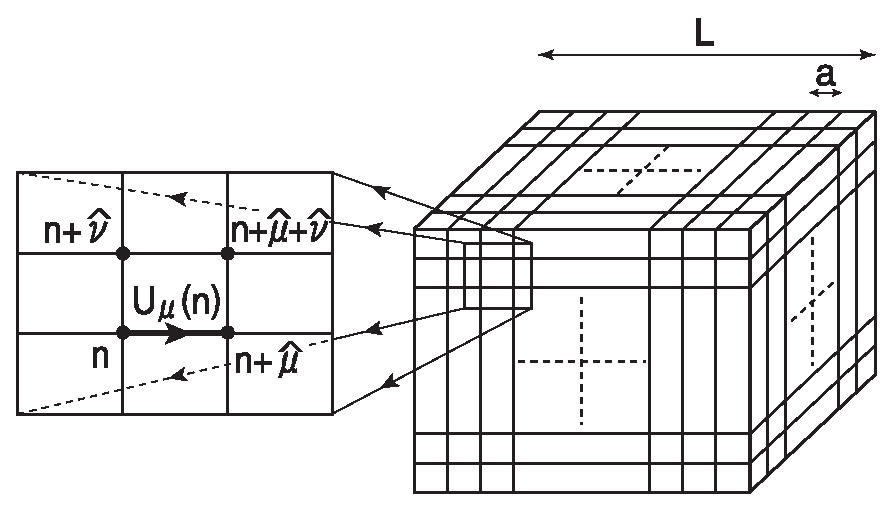
\includegraphics[scale=0.6]{Chapter3-figures/cube.eps}
 \end{center}
\caption{A hypercubic lattice in Euclidean spacetime with
 a lattice constant $a$ and the lattice size $L$.
 Quarks $q(n)$ (gluons $U_{\mu} (n)$ ) are
 defined on the sites (links).}
\label{fig:cube}
\end{figure}
%%%%%%%%%%%%%%%%%%%%%%%%%%%%%%


Let us consider a four dimensional  hyper-cubic lattice
 with a lattice spacing $a$ and the four dimensional volume $L^4$.
 Each lattice site is specified by  $n_{\mu}$ corresponding to the
 Euclidean coordinates through $x_{\mu} = a n_{\mu}$ (see Fig.\ref{fig:cube}).
   The {\it link variable} (the shortest  Wilson line on the lattice) is an SU(3)
 matrix connecting the neighboring sites $n$ and $n + \hat{\mu}$,
\beq
\label{eq:5.wilson-link}
U_{\mu}(n) = {\rm exp} \left(  ig a A_{\mu} (n) \right) .
\eeq
 Here $\hat{\mu}$ implies a vector  pointing the 
 direction of $\mu$ with a length $a$. 
 Since it is the minimal
     Wilson line, we do not need the path ordering symbol ${\rm P}$.
   Also, any non-minimal Wilson line on the lattice  is represented by a
    product of link-variables.  For later purpose, we introduce the link variable pointing the 
    opposite direction as  $U_{-\mu}(n+\hat{\mu}) = [U_{\mu}(n)]^{\dagger}$.

Let us now  define the smallest closed loop;
\beq\label{eq:5.wilson-plaq}
 U_{\mu \nu}(n) = 
 U_{\nu}^{\dagger}(n) U_{\mu}^{\dagger}(n+ \hat{\nu} ) 
  U_{\nu}(n+ \hat{\mu} )U_{\mu}(n ).
\eeq
Under local gauge
 transformation (rotation under  arbitrary  SU(3) matrix $V(n)$), we have 
\beq
 U_{\mu}(n) \rightarrow  V(n) U_{\mu}(n) V^{\dagger}(n+\hat{\mu}), \ \ 
 U_{\mu \nu}(n) \rightarrow  U_{\mu \nu}^V(n)=V(n) U_{\mu \nu}(n) V^{\dagger}(n),
 \eeq
which are the  direct consequence of Eq.(\ref{eq:5.wilson-line-iii}).

In the naive continuum limit where $a \rightarrow 0$, we have
\beq
 \label{eq:5.wilson-plaq-cont}
 U_{\mu}(n) -1 
   &=& iga A_{\mu}(n)  + O(a^2), \\
 \label{eq:5.wilson-plaq-cont-2}
 U_{\mu \nu}(n) -1 
  &=& \exp \left( iga^2 t^b (G_{\mu \nu}^b(n) + O(a^3) ) \right) -1
  = ig a^2 G_{\mu \nu}(n)  + O(a^4), \\
{\rm tr} \left(    U_{\mu \nu}(n) -1 \right) 
 &=&   {\rm tr} \left[  iga^2 t^b (G_{\mu \nu}^b(n) + O(a^3)) - \frac{1}{2} g^2 a^4 G_{\mu \nu}(n)^2 + O(a^5) \right] \nonumber \\ 
 &=& - \frac{1}{4} g^2 a^4 (G_{\mu \nu}^b(n))^2 + O(a^5) .
\eeq
Here  Eq.(\ref{eq:5.wilson-plaq-cont-2}) is obtained by 
 using the Baker-Campbell-Hausdorff formula, 
  ${\rm exp}X\cdot {\rm exp}Y =
  {\rm exp}(X + Y + [X,Y]/2 + \cdot \cdot \cdot )$.  (Exercise \ref{prob:2}). 


Finally, 
a  gluon action on the lattice, which reduces to the Yang-Mills
 action in the leading order of the  naive continuum limit ($a \rightarrow 0$), reads
\beq
\label{eq:5.wilson-action-cont}
 S_{\rm G}  &=& \beta \sum_{\rm Pl} \left[ 1 - \frac{1}{N_c} {\rm Re} \ {\rm tr} \ U_{\mu \nu}(n) \right] \\
 &=& \beta  a^4 \sum_n \sum_{\mu < \nu} \left[ 1 - \frac{1}{2N_c} {\rm tr}  \left( U_{\mu \nu}(n) +  U_{\mu \nu}^{\dagger}(n) \right) \right] \nonumber \\
 & = & \frac{1}{g^2} \sum_n \sum_{\mu \neq \nu} {\rm tr} \left[ 1 -U_{\mu \nu} (n) \right] 
  \ \ \ \ \xrightarrow{a\rightarrow 0}   \ {1 \over 4} \int d^4x  \ G_{\mu \nu}^b (x)^2 , \nonumber
 \eeq
where $\sum_{\rm Pl} $ is a sum over all non-oriented {\it plaquettes} (minimum square tile on the lattice with the area $a^2$). 
Note that  $\beta \equiv \frac{2N_c}{g^2}$ with $N_c$ being the number of colors ($N_c=3$ for QCD) 
 should not be  confused with the inverse temperature. 
    The lattice gluon action is not unique in the sense
 that one may add arbitrary non-minimal terms which vanish
 in the continuum limit ($a\rightarrow 0$).
  
%============================
\subsection{Lattice fermions}
%============================

There exist three types of gauge invariant objects made of nearest neighbor fermions as shown in Fig.\ref{fig:wilson-line}(b);
\beq
\label{eq:5.nn-link}
\bar{q}(n) q(n), \ \ 
\bar{q}(n+\hat{\mu}) U_{\mu}(n) q(n), \ \
\bar{q}(n-\hat{\mu}) U_{-\mu}(n) q(n).
\eeq
Here one may put any $\gamma$-matrices  between $\bar{q}$ and $q$
 without spoiling the color gauge invariance.
A special combination of the above   terms is called the Wilson's fermion action 
\beq
\label{eq:5.wilson-fermion}
\! \! \! 
S_{\rm F}
 &=& a^4 \sum_n 
  \left[
    m   \bar{q}(n)q(n) - \frac{1}{2a}
    \sum_{\pm \mu} \bar{q}(n+\hat{\mu}) {\Gamma}_{\mu} U_{\mu}(n) q(n)   
    - \frac{r}{2a} \sum_{\pm \mu}   \left( \bar{q}(n+\hat{\mu}) U_{\mu}(n) q(n) - \bar{q}(n)q(n) \right) 
  \right]  \nonumber \\ 
\label{eq:5.wilson-fermion2}
 & \equiv & a^4 \sum_{n',n} \bar{q}(n')
 \left( m \delta_{n',n} + D_{_{\rm W}}(n',n;U) \right) q(n)  \\
 \label{eq:5.wilson-fermion3}
 & & \xrightarrow[a \rightarrow 0] \ \  \int d^4x\  \bar{q} (x)  \left(\Gamma_{\mu} D_{\mu} + m - \frac{ar}{2} D_{\mu}^2 \right)   q(x),
\eeq
where the Wilson's Dirac operator in Eq.(\ref{eq:5.wilson-fermion2})  with the Wilson's parameter $r$ reads
\beq
\label{eq:5.wilson-dirac}
D_{\rm W}(n',n;U) 
  = - \frac{1}{2a} \sum_{\pm \mu}
 \left[
 \delta_{n',n+\hat{\mu}} (r+ {\Gamma}_{\mu} ) U_{\mu}(n)
   - r \delta_{n',n}
 \right]      .
\eeq
 To take the continuum limit in Eq.(\ref{eq:5.wilson-fermion3}), 
we use  the midpoint prescription,  $(f(x+a)-f(x-a))/2a = f'(x) + O(a^2)$
 and $(f(x+a)+f(x-a) -2f(x))/a^2 = f''(x) + O(a^2)$.
 One of the important properties of $ D_{\rm W}(n',n;U) $ is its $\Gamma_5$ Hermiticity (Exercise  \ref{prob:3}),
 \beq
 \label{eq:gamma5-hermite}
 \Gamma_5 D_{\rm W} \Gamma_5 = D_{\rm W}^{\dagger},
 \eeq
where $\Gamma_5$ is given in Appendix [Four vectors and Dirac matrices].  Note that the 
 Hermitian conjugate is taken for color, spin and  spacetime.
 
The dispersion relation (relation between the energy and momentum)
for free fermion can be obtained from Eq.(\ref{eq:5.wilson-fermion}) by taking $U_{\mu}=1$ (or equivalently $g=0$)
and substituting  the Fourier transform,
$q(n) = \int_{-\pi/a}^{\pi/a} \frac{d^4p}{(2\pi)^4} e^{i p_{\mu} n_{\mu}} q(p)$.
 This leads to $S_{\rm F}^{\rm (free)}= \int \frac{d^4p}{(2\pi)^4} \bar{q}(-p) {\cal G}_{\rm F}^{-1} q(p)$ with the
 free fermion propagator (Exercise  \ref{prob:4}),
 \beq
 \label{eq:DF}
 {\cal G}_{\rm F} (p) &=& \frac{-i  \sum_{\mu} \bar{p}_{\mu} \Gamma_{\mu}  + m(p) }{\sum_{\mu} \bar{p}_{\mu}^2 + m^2(p)},  \\
 \label{eq:Mp}
 \ \ \ \ \bar{p}_{\mu} &=& \frac{1}{a} \sin (p_{\mu} a), \ \  m(p)  =  m(0) + \frac{r}{a}  \sum_{\mu}      \left( 1-\cos (p_{\mu} a) \right)  .
 \eeq
Since $\sin (p_{\mu} a)$ becomes zero
 for $p_{\mu}a$=$(0,0,0,0)$, $(\pi, 0,0,0)$,$ \cdot $
  $(0,\pi,\pi,\pi)$, $(\pi,\pi,\pi,\pi)$, there arise
  $2^4 =16$ degenerate fermions  if we take  $r=0$.
 This is called the fermion doubling problem on the 
 lattice. In fact, there is a no-go theorem
 by  Nielsen and Ninomiya: 
 The  fermion doubling always exists, if the free fermion action  on the lattice
 has (i) bilinearity in quark field, 
  (ii) translational invariance,
   (iii) hermiticity (in the Minkowski spacetime),
    (iv) locality in spacetime, and (v) exact chiral symmetry.
Indeed, (i)-(v) are all satisfied for $r=0$.

The doubling in the dispersion relation in  the Minkowski spacetime is easily seen by Wick rotating 
$p_4 \rightarrow i E$ in Eq.(\ref{eq:DF}).  As an illustration, let us take the case with massless fermion ($m(0)=0$)
in (1+1)-dimension.  Then, the zero of the denominator after the Wick rotation for small $a$ gives,
\beq
E^2(p) \simeq \left( \frac{1}{a} \sin (pa) \right)^2 + \left( \frac{r}{a}  (1-\cos(pa)) \right)^2 ,
\eeq
whose positive energy solution is plotted in Fig.\ref{fig:dispersion} for several values of $r$.
One finds that the unphysical massless pole at $pa=\pi$ is lifted up as $r$ increases.

% FIG %%%%%%%%%%%%%%%%%%%%%%%%%%
\begin{figure}[t]
\begin{center}
%\framebox[74mm]{\rule[-26mm]{0mm}{52mm}}
\includegraphics[scale=0.75]{Chapter3-figures/dispersion.eps}
 \end{center}
\caption{The  dispersion relation for massless fermion in (1+1)-dimension on the lattice for different values of 
 the Wilson's parameter $r$.  The linear dispersion in the continuum ($E=p$) is also shown for comparison.}
\label{fig:dispersion}
\end{figure}
%%%%%%%%%%%%%%%%%%%%%%%%%%%%%% 
 
 In general, $r\neq 0$  leads to a mass splitting   of 16 fermions:
$    m(p)  \simeq  m(0)\  (^{\forall }p_{\mu} \rightarrow 0) $ and 
$m(p)= m(0) +  \frac{2r}{a}N_{\pi}  \   (^{\exists }p_{\mu} \rightarrow \pi/a) $,
 where $N_{\pi}(=1,2,3,4)$ being the number of $\pi$'s
 in  $p_{\mu}a$.  This implies that we can select only one light
 fermion by choosing $m(0) \simeq 0$ and all the other
 15 fermions have masses of $O(1/a) $  for positive  $r$.  
 A price to pay  is that the non-vanishing  $r$ breaks chiral symmetry
 explicitly for finite $a$, i.e. $\{ \gamma_5, D_{\rm W} \} \neq 0$ even for $m(0)=0$.   
  Namely, the Nielsen-Ninomiya's no-go theorem is evaded by breaking the condition (v).

  Better way to  evade the no-go theorem 
  is to break the condition (v)  in a way that the definition of
 chiral symmetry is modified.  
 Suppose we consider a modified chiral rotation in the flavor space,
 \beq
 \label{eq:5.mod-chiral}
 q \rightarrow   {\rm e}^{-i \theta_{\rm {_A}} \hat{\Gamma}_5   } q, 
  \ \ \bar{q} \rightarrow \bar{q} {\rm e}^{-i \theta_{\rm {_A}} \Gamma_5 }  \ \ 
   {\rm with} \ \  \hat{\Gamma}_5 =  \Gamma_5 (1-2 a D_{_{\rm GW}})  ,
\eeq
which  reduces to the standard axial rotation for $a\rightarrow 0$.
Here  $D_{\rm GW}$ is a generalized Dirac operator which is 
 constructed so that   
  $\bar{q} D_{\rm GW} q$ is  invariant under
 Eq.(\ref{eq:5.mod-chiral}) even for finite $a$;
\beq
 \label{eq:5.GW-1}
\Gamma_5 D_{\rm GW} + D_{\rm GW} \hat{\Gamma}_5 =0 ,
\eeq
or equivalently  $\{ \Gamma_5, D_{_{\rm GW}} \} 
 = 2a D_{_{\rm GW}} \Gamma_5 D_{_{\rm GW}}$.
 This     is called the Ginsparg-Wilson relation.
  An explicit form of $D_{\rm GW}$ may be constructed as
\beq
 \label{eq:5.overlap-op}
 D_{\rm GW} = 
 \frac{1}{2a} \left( 1+  \frac{X}{\sqrt{X^{\dagger}X}} \right)  \ \  
 {\rm with} \ \ 
 X \equiv   D_{\rm W}^{(r=1)} - m_0  ,
\eeq
where $m_0 a$ being a dimensionless parameter of $O(1)$.
 Unlike the case of $m$ in the Wilson fermion,
 $m_0$  is not directly related to the physical fermion mass.
 Nevertheless,  if we choose the region $0< m_0 a < 2$,  
  there exists
 an  exact massless mode for $N_{\pi}=0$ for finite $a$,
 and  other 15 modes have a large mass 
 $(2/a)(2N_{\pi}-m_0 a)>0$.   (Exercise  \ref{prob:5}).
 
 Going back to the Wilson's fermion action, Eq.(\ref{eq:5.wilson-fermion}).
it  can be  conveniently rewritten  as 
\beq
 \label{eq:5.wilson-fermion-lat}
S_{\rm F}    
    & = & \sum_{n',n} \bar{\psi}(n') F(n',n;U) \psi(n) ,\\
\label{eq:5.wilson-fermion-op}
F(n',n;U) &=& \delta_{n'n} 
- \kappa \sum_{\pm \mu} \delta_{n',n+\hat{\mu}}
 (r + {\Gamma}_{\mu}) U_{\mu}(n),
\eeq
where we have redefined the quark field 
 as $\psi = a^{3/2} q /\sqrt{2\kappa }$ with
 $\kappa = [2(ma + 4r)]^{-1}$
 being the  {\it hopping parameter}. 
  If the quark mass $m$ is large, $\kappa$ is
 small and the ``hopping" to the 
  neighboring lattice site is suppressed.
   
%=================================
\subsection{Partition function on the lattice}
%=================================

The functional integration over quarks and gluons in continuum QCD
in Eq.(\ref{eq:Z-QCD}) is now transformed to the integration over quarks 
  on each site and gluons on each link in lattice QCD. 
 With Eq.(\ref{eq:5.wilson-action-cont}) and
   Eq.(\ref{eq:5.wilson-fermion-lat}), the partition function without the external field ($J=0$) reads
\beq
\label{eq:5.lattice-Z}
{\cal Z}  =  \int[dU d\bar{\psi}d\psi]   {\rm e}^{-  S_{\rm G}(U) - S_{\rm F}(\bar{\psi},\psi,U) }  
    =  \int[dU]\ {\rm Det}\ F(U) \ {\rm e}^{- S_{\rm G}(U) }
    = \int[dU]\  \ {\rm e}^{- S_{\rm eff}(U) }
\eeq
To obtain the second equality, we have explicitly carried out the integration over the
 Grassmann variables, $\bar{\psi}$ and $\psi$, 
 by using the formula in Appendix [Gaussian and Grassmann integrals]. Here ${\rm Det}$ implies the determinant in 
  spacetime, color, flavor and spin degrees of freedom.
In the third equality, the exponent  is defined as 
 \beq
\label{eq:Seff}
 S_{\rm eff}(U) \equiv S_{\rm G}(U) - {\rm ln Det} F(U).
 \eeq
 
 The integration over the group element $[dU] = \prod_{\mu,n} dU_{\mu}(n) $ can be defined through 
  the {\it Haar measure} $dU$ which has the property,
  $ d(V_{\rm L}U V_{\rm R}^{\dagger})=dU$
  with  $V_{\rm L,R}$ being arbitrary group elements. Such a measure is
   unique for compact groups such as SU$(N)$.
 If we parametrize the group element as $U=\exp(i \theta_a t^a)$,  one can define the 
 distance in the group space as $ds^2 = g_{ab}  (\theta) d\theta_a d\theta_b$, where the 
 metric is given by $g_{ab}=  {\rm tr} (L_aL_b) =  {\rm tr} (R_a R_b) $ with 
 \beq
 \label{eq:LR-form}
 L_a= -i U^{-1} ( {\partial} U/{\partial \theta_a}), \ \ \ 
 R_a= -i ({\partial}U/{\partial \theta_a} ) U^{-1}.
 \eeq   
 Then the Haar measure can be   explicitly written as
  \beq
  \label{eq:Haar-measure}
   dU = {\cal N} \sqrt{ \det g} \ \prod_a d\theta_a,
  \eeq
  with an overall normalization factor ${\cal N}$.
  
 The followings are some examples of the  SU($N$)  group integration, which can be proved
 by the invariant property of the Haar measure (except for the first one which determines the 
 normalization of the measure) (Exercise \ref{prob:6}):
 \beq
 \label{eq:group-int-0}
  & &   \int dU \  1  =  1 , \\ 
 \label{eq:group-int-1}
 & &   \int dU \ U_{ij}  =  0, \\
 \label{eq:group-int-2}
 & &    \int  dU \ U_{ij} U_{k\ell}^{\dagger}  =  \frac{1}{N} \delta_{i\ell} \delta_{jk} , \\
 \label{eq:group-int-4}
 & &  \int dU \ U_{ij} U_{k\ell}  U_{i'j'}^{\dagger} U_{k'\ell'}^{\dagger}
 = \frac{ \delta_{ij'} \delta_{ji'} \delta_{k\ell'} \delta_{\ell k'} + {(j' \leftrightarrow \ell',  i' \leftrightarrow k' ) }}{N^2-1}
   -  \frac{\delta_{ij'} \delta_{jk'} \delta_{k\ell'} \delta_{\ell i'} + { (j' \leftrightarrow \ell',  i' \leftrightarrow k' )}  }{N}, \\
 \label{eq:group-int-B}
 & &  \int dU \ U_{i_1 j_1} \cdots U_{i_N j_N} = 
 \frac{1}{N!} \epsilon_{i_1 \cdots i_N}    \epsilon_{j_1 \cdots j_N} .
 \eeq    

   
Similar to the statistical systems such as the Ising model, 
 observables are obtained by averaging over the statistical weight  as
 \beq
 \langle {\cal O} \rangle = \frac{1}{{\cal Z}}  \int[dU]\ {\cal O}(U) \ {\rm e}^{- S_{\rm eff}(U) }.
 \eeq
    Due to the gauge invariance of the Haar  measure,
 gauge non-invariant quantities have vanishing expectation values
  (Elitzer's theorem).  For example, consider the expectation value of the link variable,
 \beq
 \label{eq:elitzer}
 \langle U_{\mu} (n) \rangle 
 = \frac{1}{{\cal Z}}  \int [dU] U_{\mu} (n)  \ {\rm e}^{- S_{\rm eff}(U) }  = V(n)  \langle U_{\mu} (n) \rangle ,
\eeq
where we have made a change of variable, $U_{\mu}(n) \rightarrow V(n) U_{\mu}(n)$ with $V(n)$ 
being the $SU(N)$ matrix, and used the  gauge invariance of the Haar measure as well as ${\rm Det}\ F(U)$ and 
$S_{\rm G}(U)$.  Since Eq.(\ref{eq:elitzer}) must be true for arbitrary $V(n)$, we have $ \langle U_{\mu} (n) \rangle =0$.
 
Some examples of the non-vanishing  observables are shown  in Fig.\ref{fig:correlation}:
 (a) and (b) correspond to the mesic and baryonic correlations, respectively,  while (c) is a correlation related to the 
baryon-baryon interactions.  The filled circles are the spacetime points where the quarks and anti-quarks
are created or absorbed. Each  line with arrow indicates the quark propagator $F^{-1}(n,n';U)$ 
connecting two spacetime points $n$ and $n'$.  Thus, the explicit forms of the
 mesic and baryonic correlations are
 \beq
 \label{eq:correlation-M}
C_{\rm M}(n,n') 
 &=& \frac{1}{{\cal Z}}  \int [dU] \ F_{\alpha \beta}^{-1}(n,n';U) F_{\beta \alpha}^{-1}(n',n;U)  \ {\rm e}^{- S_{\rm eff}(U) } ,\\
\label{eq:correlation-B}
C_{\rm B}(n,n') 
 &=& \frac{1}{{\cal Z}}  \int [dU] \ \epsilon_{\alpha \beta \gamma} \epsilon_{\alpha' \beta' \gamma'} 
 F_{\alpha \alpha'}^{-1}(n,n';U) F_{\beta \beta'}^{-1}(n,n';U) F_{\gamma \gamma'}^{-1}(n,n';U)  \ {\rm e}^{- S_{\rm eff}(U) } ,
  \eeq
where all the color indices are contracted so that $C_{\rm M}$ and $C_{\rm B}$ are gauge invariant. 
 Other quantum numbers such as spin and flavor  associated with $F^{-1}$ are
 not shown explicitly.
  Spacetime, spin and flavor dependences of  $C_{\rm M}(n,n')$ in (a) and $C_{\rm B}(n,n')$ in (b)
  have all the information on the hadronic states in various different channels, while
  $C_{\rm BB}(n,m,n',m')$   in (c) has the information on baryon-baryon interactions.
      
% FIG %%%%%%%%%%%%%%%%%%%%%%%%%%
 \begin{figure}[t]
%\vspace{-1cm}
\begin{center}
%\framebox[74mm]{\rule[-26mm]{0mm}{52mm}}
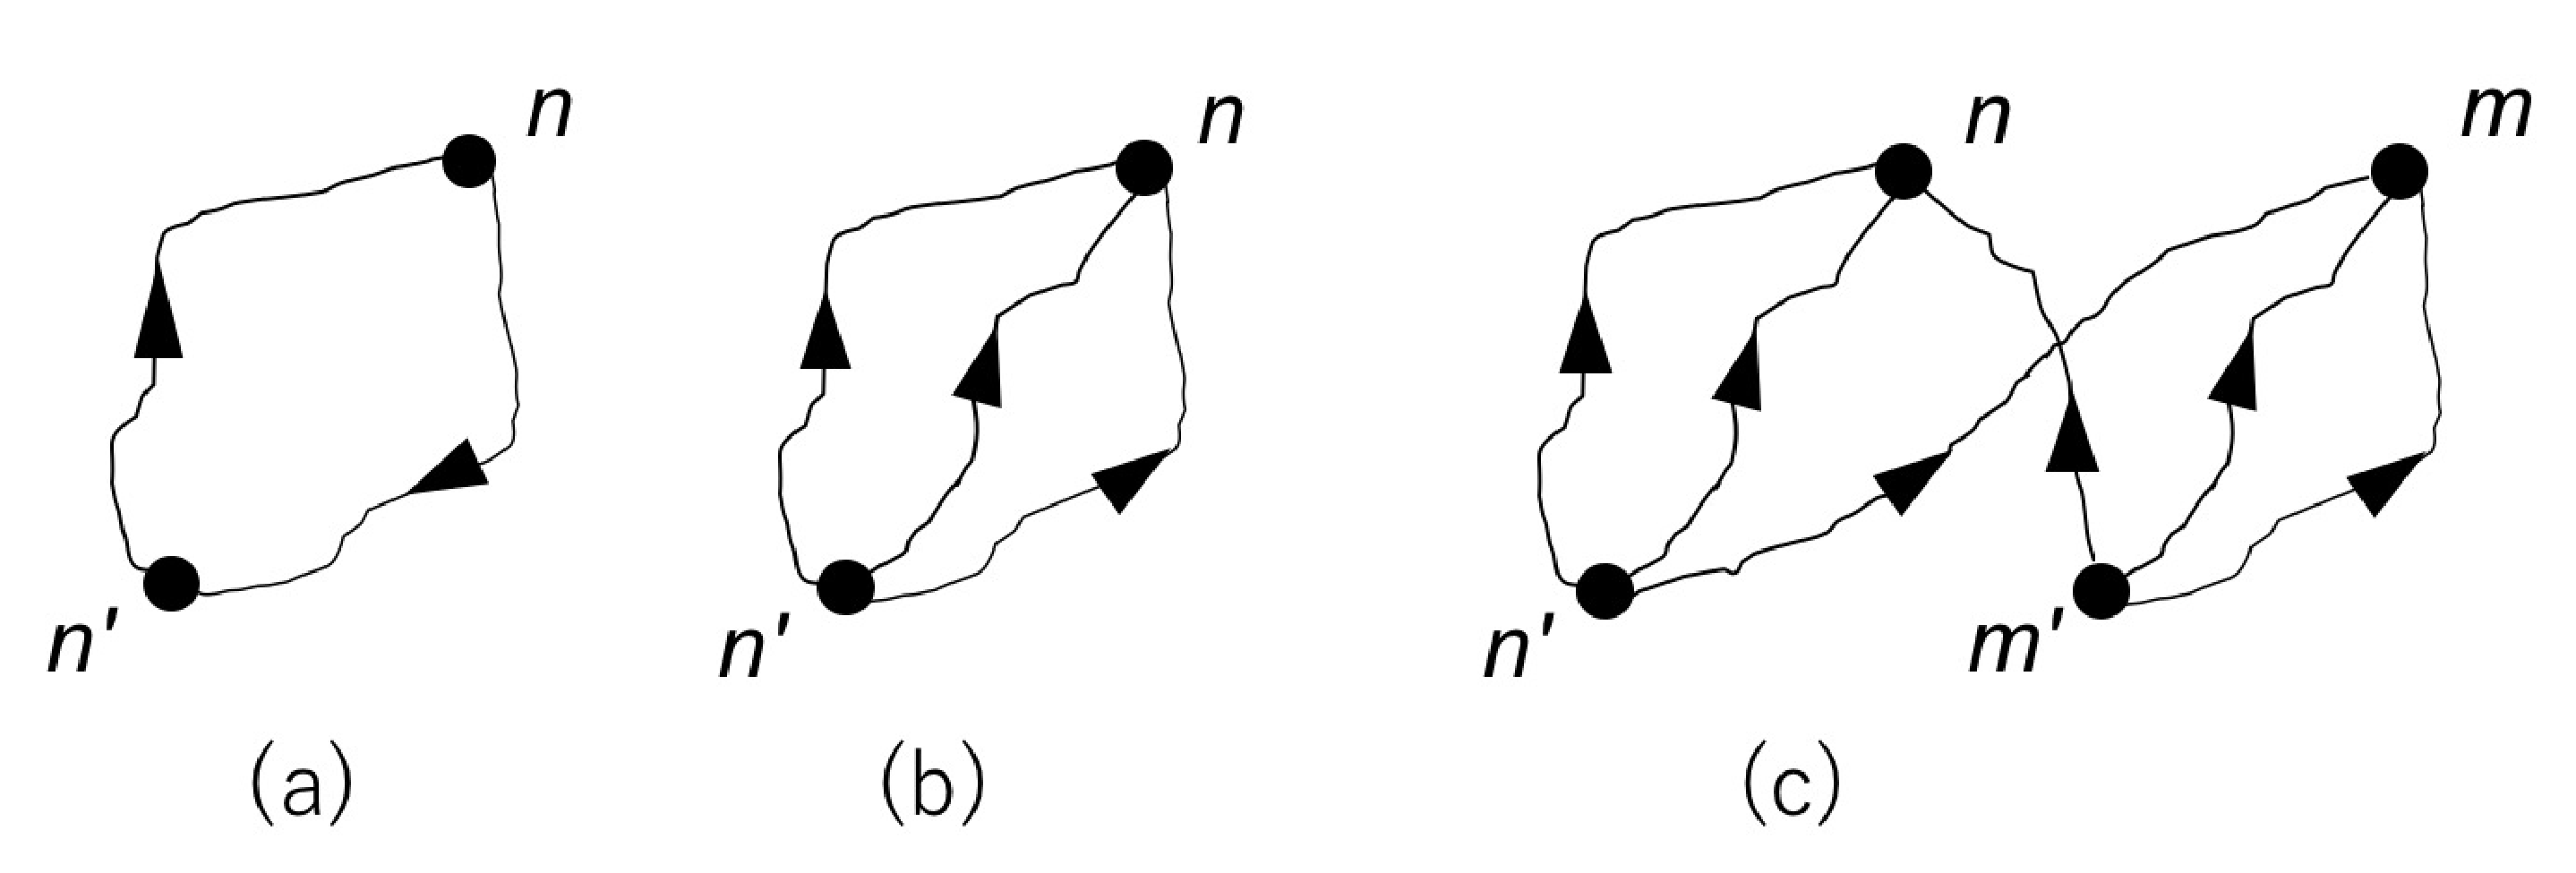
\includegraphics[scale=0.2]{Chapter3-figures/correlations.eps}
 \end{center}
%\vspace{-1cm}
\caption{
(a) Single meson correlation representing the propagation of a  meson created at point $n'$ and absorbed at point $n$.
(b)  Single baryonic correlation representing the propagation of a  baryon created at point $n'$ and absorbed at point $n$.
(c)  Two baryon correlation which contains the information on baryon-baryon interaction.}
\label{fig:correlation}
\end{figure}
%%%%%%%%%%%%%%%%%%%%%%%%%%%%%%%
 
   
%===========================================
\subsection{Strong coupling expansion and quark confinement}
%===========================================


% FIG %%%%%%%%%%%%%%%%%%%%%%%%%%
\begin{figure}[t]
\begin{center}
%\framebox[74mm]{\rule[-26mm]{0mm}{52mm}}
\includegraphics[scale=0.55]{Chapter3-figures/wilson-L.eps}
 \end{center}
\caption{A rectangular  Wilson loop with the
 temporal (spatial) size ${\cal T}$ ($R$).}
\label{fig:wilson-L}
\end{figure}
%%%%%%%%%%%%%%%%%%%%%%%%%%%%%%

One of the remarkable properties of QCD is the   confinement of quarks inside 
hadrons.  Simplest setup to see this phenomena is to consider
the potential $V(R)$ between  an infinitely heavy quark $Q$ and an anti-quark $\bar{Q}$ with
a fixed separation $R$.
It corresponds to Fig.\ref{fig:wilson-L} and can be written as
\beq
 \label{eq:5.wilson-loop-lattice}
\langle W(C) \rangle  
 & = & \langle {\rm tr}\ \prod_{{\rm link}\in C}  U_{\mu}(n) \rangle , \\
 \label{eq:5.wilson-loop-asym}
 & \propto  & 
  {\rm e}^{-V(R) {\cal T} } \simeq 
 \exp \left[ -\left( K R + b + \frac{c}{R} + \cdots \right) {\cal T} \right] ,
\eeq  
where we  have taken a limit     
${\cal T} \gg R \rightarrow \infty$ in   Eq.(\ref{eq:5.wilson-loop-asym}).
 Remembering the fact that the real time $t$ and the imaginary time $\tau$ are
 related as  $\tau=it$, the exponential falloff of  $\langle W(C) \rangle$ in $\tau$ implies the 
  temporal oscillation in $t$, and its $R$-dependent coefficient is nothing but the 
 interaction  energy between $Q$ and $\bar{Q}$.  
 
In Eq.(\ref{eq:5.wilson-loop-asym}), 
   $K > 0$  implies 
 the existence of a string-like
linear confining potential.
 It also implies 
 the area law  of the Wilson loop 
 $\langle W(C) \rangle \sim \exp(-K{\cal A})$
 where ${\cal A}= R \times {\cal T} $ is 
  the area inside the path $C$.
    In full QCD where pair creation of light quarks 
 are allowed,  
  the linear rising potential becomes eventually 
    flat at long distances due to the breaking of the string,
  $Q\bar{Q} \rightarrow (Q\bar{q})(q\bar{Q})$.
  
  To make the analysis simple, let us now consider the 
  SU$(N_c)$ Yang-Mills theory
  without light quarks: This is called the quenched 
  approximation and corresponds to take $F(U) =1$.
In this case,  the Wilson loop can be evaluated analytically
 in the strong coupling regime ($g \rightarrow \infty$).
First of all,  $S_{\rm G}$ is proportional to $1/g^2$,
so that  one can make an expansion,  
$\exp (-S_{\rm G}) = 1 - S_{\rm G}+ S_{\rm G}^2 /2 + \cdots $
 and finds (Exercise \ref{prob:7})
\beq
\label{eq:5.wilson-strong}
\langle W(C) \rangle = {1 \over {\cal Z}}
 \int [dU] \ {\rm tr} \prod_{{\rm link}\in C} U_{\mu}(n) \  
 \sum_{\ell =0}^{\infty} \frac{1}{\ell !} (-S_{\rm G})^{\ell}.
\eeq
 
Only the first three integrals, Eqs.(\ref{eq:group-int-0},\ref{eq:group-int-1},\ref{eq:group-int-2}),
 are necessary to extract the leading contribution to 
 $\langle W(C) \rangle $  in the strong coupling.
   Key observation is that all the $U$'s 
  from the Wilson loop and $U^{\dagger}$'s 
 from $(-S_{\rm G})^{\ell}$ should be paired in the leading order of $1/g^2$
 in   Eq.(\ref{eq:5.wilson-strong}).
  This means that the area inside the Wilson loop is tiled up 
 with minimum number of plaquettes as shown in
  Fig.\ref{fig:strong-c}. All the structures other than 
  the minimal surface are higher orders in  $1/g^2$.

% FIG %%%%%%%%%%%%%%%%%%%%%%%%%%
 \begin{figure}[t]
\begin{center}
%\framebox[74mm]{\rule[-26mm]{0mm}{52mm}}
\includegraphics[scale=0.65]{Chapter3-figures/strong-c.eps}
 \end{center}
\caption{A minimum surface in which the Wilson loop is tiled 
   up by the fundamental plaquettes in the 
 strong coupling limit.}
\label{fig:strong-c}
\end{figure} 
%%%%%%%%%%%%%%%%%%%%%%%%%%%%%%

 In the evaluation of the numerator of
 Eq.(\ref{eq:5.wilson-strong}), 
 each plaquette has a contribution $1/g^2$. 
 Also each  integration on the link
   gives a factor $1/N_c$
   and the contraction of the color indices gives a factor $N_c$
 on each  site.
  On the other hand,
 ${\cal Z}$  (the denominator of Eq.(\ref{eq:5.wilson-strong})
 is   unity in the leading order. 
    Thus, one arrives at the formula in the lowest order
 of the strong coupling expansion,
\beq
 \label{eq:5.strong-estimate}
\frac{1}{N_c} \langle W(C) \rangle 
& & \xrightarrow[g^2\rightarrow \infty] 
 \  \frac{1}{N_c} \cdot  
\left(\frac{1}{g^2} \right)^{N_{\rm plaq}} \cdot  
\left(\frac{1}{N_c} \right)^{N_{\rm link}} \cdot N_c^{N_{\rm site}}  , \nonumber \\
& & \ \ \ \ \ \ \ \ \ \ \ =\left(\frac{1}{N_c g^2} \right)^{\frac{R {\cal T}}{a^2}} 
= \exp \left( - \frac{\ln N_c g^2}{a^2} R {\cal T} \right) ,
\eeq
where we have used a relation, $N_{\rm link}-N_{\rm site}+1 
 = N_{\rm plaq}$ and 
$N_{\rm plaq} a^2 = R {\cal T} ={\cal A}$.
 Since it shows the area law, \index{area law}
  the confinement is naturally obtained in the strong coupling
  with the linear rising potential, 
\beq
 \label{eq:5.linear-potential}
V(R) = K R \ \ {\rm with} \ \ K = \frac{1}{a^2} \ln (N_c g^2).
\eeq

 If we consider higher orders of the strong coupling expansion,
   ``rough" surfaces should be taken 
 into account.
 Nevertheless, the confining feature is
 stable against small perturbations in $1/g^2$.
  In fact, there exits a theorem 
  that,  for sufficiently large $g$, the strong coupling expansion 
  converges and shows confinement for all compact gauge groups  
  in all spacetime dimensions.
  

  A question here is that whether the real world 
  corresponds to the strong coupling region discussed above.
  The answer is no;  the real world corresponds to  the weak coupling regime. 
  For compact QED (quantum electrodynamics
  formulated in terms of the  U(1) link variable),
  the confinement  $K>0$ in the strong coupling regime 
   changes to  $K=0$ in the weak coupling regime.
  On the other hand,  in QCD in four spacetime dimensions 
 with $N_c=3$,   the confinement feature is expected to persist even in the weak coupling regime. 
 Indeed, there are  strong evidences for this statement 
  from  LQCD simulations.
  Its analytic proof, however,  is  still missing and is being one of the 
   most challenging problems in mathematical  physics.
   

%===============================================
\subsection{Weak coupling expansion and continuum limit}
%===============================================

  Lattice QCD can be regarded as an effective field theory
   with an ultraviolet (UV)  cutoff in the coordinate space. 
   The gauge coupling  $g$ is then interpreted as
  a bare coupling defined at the scale $a$ where
  quantum fluctuations with the wave length shorter than 
  $a$ are integrated out.  In non-Abelian gauge theories,
   it can be shown that $g(a)$ decreases logarithmically as $a$ decreases
   unless the number of matter fields is not too large.  
    This is called the {\it asymptotic freedom}, and is essential for taking
    the continuum limit ($a \rightarrow 0$) to remove the 
    lattice artifact. 
        
 For simplicity, let us consider the case with massless fermions, where 
 observables
   ${\cal O}$ such as the string tension and the hadron masses  depend only
   on the coupling $g$ and the  regularization scale $a$. 
   Then,  from the dimensional ground, one can  write  
     \beq
\label{eq:5.O-dim}
 {\cal O} (g(a),a) = a^{-d} X(g(a)),
 \eeq
 where $d$ is the mass-dimension of ${\cal O}$ and $X$ is a dimensionless
 function of $g$.  The $a$-independence of the observable implies
 \beq
\label{eq:5.O-RG}
 a{d{\cal O} \over da} 
  =  
  \left( a \frac{\partial}{\partial a} 
 - \beta_{_{\rm LAT}}  \frac{\partial}{\partial g} \right) {\cal O}(g(a), a)  = 0 , 
\ \   \beta_{_{\rm LAT}}(g) =  -a {dg(a) \over da} .
\eeq
By integrating the first equation in Eq.(\ref{eq:5.O-RG}),  we find
\beq
\label{eq:5.lat-F}
 X(g) = 
 \exp \left( -d \int^g {dg' \over \beta_{_{\rm LAT}}(g')} \right) .
 \eeq
Suppose that 
 the beta-function can be expanded in terms of $g$ for small $a$:
$\beta_{_{\rm LAT}}(g)   = 
  - \beta_0 g^3 - \beta_1  g^5 + \cdot \cdot \cdot $. Here
  $\beta_0$ and $\beta_1$ can be shown to be independent of the 
   regularization scheme and are known to be 
\beq
\beta_0= \frac{1}{(4\pi)^2} \left( \frac{11N_c}{3}-\frac{2N_f}{3} \right),
\ \ \  \beta_1= \frac{1}{(4\pi)^4} \left( \frac{34N_c^2}{3}-\frac{38N_f}{3} \right),
\eeq
           for QCD with $N_c$ colors and     $N_f$ fermions.
  
% FIG %%%%%%%%%%%%%%%%%%%%%%%%%%
 \begin{figure}[t]
\begin{center}
%\framebox[74mm]{\rule[-26mm]{0mm}{52mm}}
%\includegraphics[scale=0.6]{as-scale.eps}
\includegraphics[scale=0.30]{Chapter3-figures/crossover.eps} 
 \end{center}
\caption{Crossover behavior of the dimensionless
 string tension $Ka^2$ from the strong coupling
 regime  $\beta=2N_c/g^2 \rightarrow 0$ to the weak coupling
  (asymptotic scaling) regime  $\beta=2N_c/g^2 \rightarrow \infty$
  for SU($N_c=2$) Yang-Mills theory.  The figure is adapted from
  \cite{Creutz:1980zw}.
  }
\label{fig:as-scale}
\end{figure}
%%%%%%%%%%%%%%%%%%%%%%%%%%%%%%%%

        
By integrating  the second equation in Eq.(\ref{eq:5.O-RG}) with the above expansion of
$\beta_{_{\rm LAT}}(g)$, one finds  
 \beq
\label{eq:5.a-vs-L}
 a = \Lambda_{_{\rm LAT}}^{-1} \cdot  
 \exp  \left( -\frac{1}{2\beta_0 g^2}  \right)  \cdot
  (\beta_0 g^2)^{-{\beta_1 \over 2 \beta_0^2}} 
 \cdot (1 + O(g^2)).
 \eeq
Here  $ \Lambda_{_{\rm LAT}}$ is called the scale parameter on the lattice, and  
   $g(a)$ can be expressed in terms of $a$ and $ \Lambda_{_{\rm LAT}}$ ((Exercise \ref{prob:8}),
 \beq
\label{eq:5.lat-running-g}
{1 \over g^2(a)} = \beta_0 \ln \left( 1 \over a^2  \Lambda_{_{\rm LAT}}^2 \right)
+ {\beta_1 \over \beta_0} \ln \ln \left( 1 \over a^2  \Lambda_{_{\rm LAT}}^2 \right)
+ \cdot \cdot \cdot .
\eeq
 This is the asymptotic freedom
 in which $g(a)$ decreases as $a$ decreases.  This also justified the 
 assumption that the beta-function can be expanded by $g(a)$ for small $a$.
 
 
Direct way to extract the actual value of $ \Lambda_{_{\rm LAT}}$  is to
 carry out  numerical simulations of  
 a certain physical quantity (such as the string tension)
 and compare the result with the experimental value. 
 For example, the string tension, which has mass-dimension
 two ($d=2$) should  behave as
\beq
\label{eq:5.lat-K}
K a^2 = C_K \exp \left( - {1 \over \beta_0 g^2} \right) 
(\beta_0 g^2)^{-\beta_1 /\beta_0^2} = C_K  \Lambda_{_{\rm LAT}}^2 ,
\eeq
with $C_K$ being a dimensionless numerical constant independent
 of $g$.  As  can be seen from this example, 
 the functional form of the physical quantities 
 for $g\sim 0$  is  severely constrained.  
This is called the {\em asymptotic scaling} which 
 is used to check whether the system is 
  close enough to the continuum limit.
Shown in Fig.\ref{fig:as-scale} is a historic numerical study, which shows 
 a crossover of $Ka^2$  from the strong coupling regime to the weak coupling regime
 in SU(2) Yangs-Mills theory. 
  


%===============================
\subsection{Running coupling}
%===============================

% FIG %%%%%%%%%%%%%%%%%%%%%%%%%%
\begin{figure}[t]
\begin{center}
%\framebox[74mm]{\rule[-26mm]{0mm}{52mm}}
%\includegraphics[scale=0.6]{as-scale.eps}
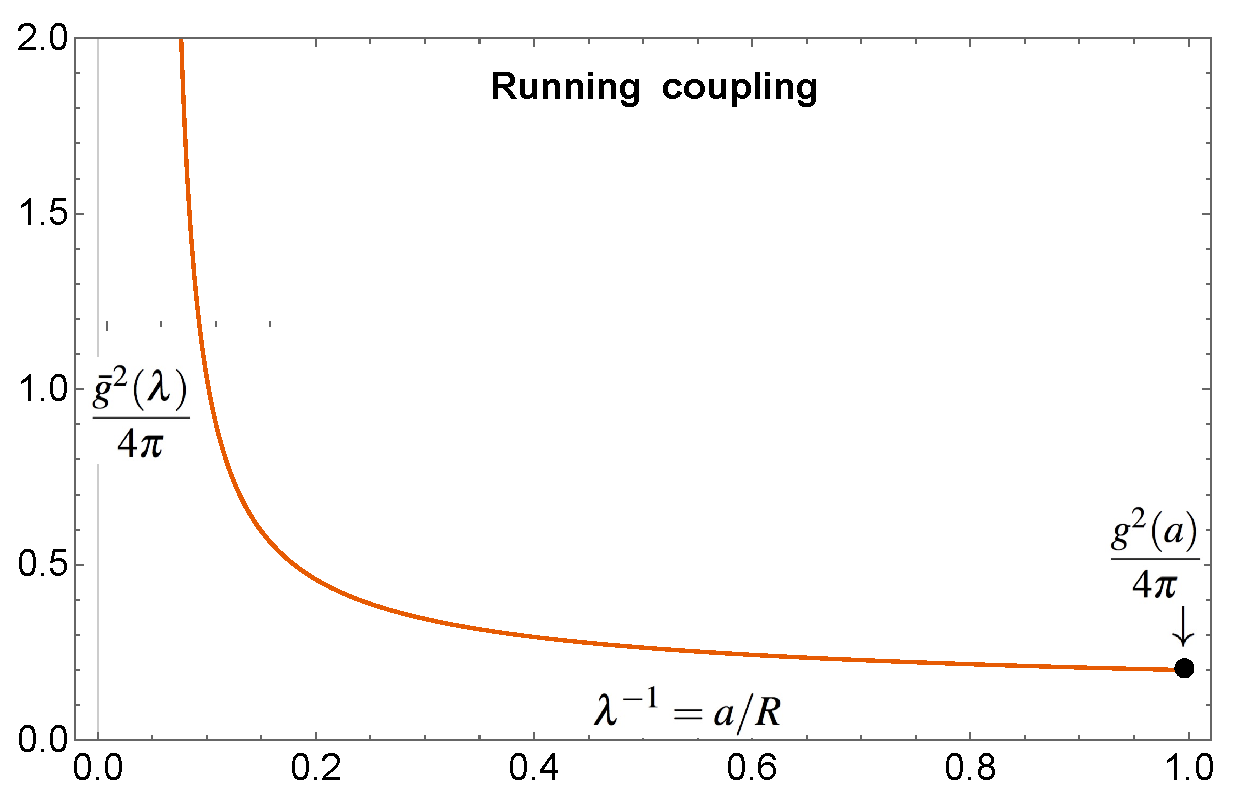
\includegraphics[scale=0.45]{Chapter3-figures/running-g.eps} 
 \end{center}
\caption{Perturbative running coupling $\frac{1}{4\pi}\bar{g}^2(\lambda)$ as a function of $\lambda^{-1}$.
In the short distance limit ($\lambda =1$), the running coupling coincides with the bare coupling $\bar{g}(\lambda=1)=g(a)$,
while, in the long distance regime ($\lambda \ll 1$), the running coupling grows. }
\label{fig:running-g}
\end{figure}
%%%%%%%%%%%%%%%%%%%%%%%%%%%%%%%


Let us now consider an observable ${\cal O}$ which depends 
not only on $g(a)$ and $a$ but also on some external dimensionful parameter.
For concreteness, we consider the heavy quark potential $V(R; g(a),a)$ in the 
quenched approximation.  Since it has the dimension of energy, one may write
\beq
V(R,g(a),a) = R^{-1} \tilde{V} (R/a, g(a)).
\eeq
Then the cutoff independence of the observable, $a \frac{d}{da}V(R,g(a),a)=0$,  leads to
\beq
\left( \lambda \frac{\partial}{\partial \lambda} + \beta_{_{\rm LAT}} \frac{\partial}{\partial g} \right) \tilde{V} (\lambda,g)=0,
\label{eq:RG-R}
\eeq
where we have introduced 
a dimensionless  scaling parameter $\lambda$ through $R=\lambda a$.

]The solution of the {\it renormalization group equation}, Eq.(\ref{eq:RG-R}), reads
\beq
\label{eq:RG-sol}
 \tilde{V} (\lambda,g(a)) = \tilde{V} (1, \bar{g}(\lambda)).
 \eeq
 Here $\bar{g}(\lambda)$ is called the {\it running coupling} which is  a solution of
\beq
\lambda \frac{d\bar{g}}{d\lambda}  = - \beta_{_{\rm LAT}} (\bar{g}(\lambda)),
\eeq
with the boundary condition, $\bar{g}(\lambda=1)= g(a)$.
One can show that  Eq.(\ref{eq:RG-sol})  satisfies Eq.(\ref{eq:RG-R}) explicitly by applying the partial derivatives 
 or more generally by the method of characteristics in Appendix [Method of characteristics].
Then, we eventually arrive at the formula 
\beq
V(R,g(a), a) = \frac{a}{R} V (a, \bar{g}(R/a), a) .
\eeq
If $R$ is  in the interval,  $a < R \ll  \Lambda_{_{\rm LAT}}^{-1}$, the running coupling $\bar{g}$ is small enough, so that 
one may use the perturbative expansion of $\beta_{_{\rm LAT}}$ to obtain
\beq
\bar{g}^2(R/a) \simeq \frac{g^2(a)}{1-2\beta_0 g^2(a) \ln (R/a)} =  \frac{1}{2\beta_0 \ln (1/(R \Lambda_{_{\rm LAT}}) ) }. 
\label{eq:running-R}
\eeq 
In Fig.\ref{fig:running-g}, the behavior of $\frac{1}{4\pi}\bar{g}^2(\lambda)$  as a function of $\lambda^{-1}$ is shown.
The bare coupling $\frac{1}{4\pi}g^2(a)$ appears as the boundary condition at shortest distance $\lambda=R/a=1$,
while $\frac{1}{4\pi} \bar{g}^2(\lambda)$ grows  as $\lambda$ increases.
The latter implies that the strong interaction has anti-screening feature.

For $R$ sufficiently close to $a$, one may evaluate the potential by using perturbation theory as
$V (a, \bar{g}(R/a), a)  = - C_{{\rm F}} \frac{\bar{g}(R/a)^2}{4\pi a}$, so that we finally obtain
\beq
\label{eq:RG-Coulomb}
V(R,g(a),a) \simeq - C_{{\rm F}} \frac{\bar{g}^2(R/a)}{4\pi R} \ \ \ \ \ (a < R \ll  \Lambda_{_{\rm LAT}}^{-1}),
\eeq
where $C_{{\rm F}}=4/3$ for $N_c=3$ is given in Appendix [SU($N$) algebra].
Eq.(\ref{eq:RG-Coulomb}) is nothing but the Coulomb potential with the running coupling constant.
Note that the left hand side is $a$-independent, while the right hand side has
logarithmic $a$-dependence through $\bar{g}$.  This is due to the use of perturbation theory;
such a logarithmic $a$-dependence  is cancelled by the next-to-leading order term.
Note also that the similar analysis can be done for any other observables.
The QCD thermal pressure at finite temperature $P(T,g(a),a)$ is a typical example, in which 
the weak coupling analysis (i.e. the description by  quark-gluon plasma picture)
is justified  under the condition  $  \Lambda_{_{\rm LAT}} \ll T < a^{-1}$. 



%%%%%%%%%%%%%%%%%%%
\section{Lattice QCD:  numerical simulations}
%%%%%%%%%%%%%%%%%%%


Suppose we have a lattice having $N_{\rm s}$ ($N_{\tau}$) number of sites
in each spatial (temporal) direction. Then 
 the total number of links is 
   $  N_{\rm s}^3 \times N_{\tau}  \times 4$. 
 Therefore the total  number of gluon integrations $\int [dU]$
 for a moderate lattice size  $N_{\rm s} = N_{\tau} =32$ reads
\beq
\label{eq:5.lattice-size}
 ( N_{\rm s}^3 \times N_{\tau} \times 4 )_{\rm links} \times 8_{\rm
 color} \sim 3 \times 10^7 .  
\eeq 
This is hopelessly a large number for standard methods of numerical
integration.  In this case, the Monte Carlo (MC) integration, which is
a statistical way to evaluate the integral, plays a powerful role. For
rapidly varying integrand, the MC integration should be supplemented
by the importance sampling to have better accuracy, in which the
rapidly varying part is sampled more than the slowly varying part.
     
     
 %==========================
\subsection{Importance sampling}
\label{ss:IS}
%==========================
    
     Let us consider the general partition function ${\cal Z}= \int [d\phi] \exp(-S(\phi)) $,
    with some c-number field $\phi$  and try to calculate  an observable ${\cal O} $ by
  \beq
  \langle {\cal O} \rangle = \frac{1}{{\cal Z}} \int [d \phi] \ {\cal O} (\phi) e^{-S(\phi)}.
  \eeq   
  The basic procedure of the MC integration
  with the {\it importance sampling} consists of two steps:
  \begin{enumerate}
  \item[(I)]   Generate a set of field configurations, $ \{  \phi^{(1)}, \phi^{(2)}, \cdots, \phi^{(N)} \}$, 
with $\phi^{(n)}$  being arranged to appear with 
 a probability in ``equilibrium", $W_{\rm eq}[\phi]={\cal Z}^{-1} \exp (-S(\phi))$.
 \item[(II)]  The field configurations thus generated 
 are  used to calculate the expectation value,
 \beq
\label{eq:5.obs-average}
\langle {\cal O} \rangle = \frac{1}{N}\sum_{n=1}^N {\cal O}^{(n)}
\pm \sqrt{{\sigma^2 \over N}}, \ \ \ \ \ 
\sigma^2 =  \frac{1}{N-1} \sum_{n=1}^N \langle {\cal O}^{(n)} - \langle {\cal O} \rangle \rangle^2 ,
\eeq
with ${\cal O}^{(n)}={\cal O}(\phi^{(n)})$.
\end{enumerate}

 %=========================================
\subsection{Markov chain Monte Carlo (MCMC)}
%==========================================
  
 For large  number of integration variables such as Eq.(\ref{eq:5.lattice-size}), 
 it  is essential to develop an appropriate scheme to carry out  Step (I) in Sec. \ref{ss:IS}. 
 The {\it Markov chain Monte Carlo (MCMC)}  method is one of such schemes. 
    
Let us consider a chain of configurations  generated successively starting from an
initial configuration,
\beq
\label{eq:M-chain}
 \phi_{0} \rightarrow  \phi_{1} \rightarrow \phi_{2}
 \rightarrow \cdots \rightarrow \phi_{i} \rightarrow  \phi_{i+1}
\rightarrow \cdots ,  
\eeq
where the ``{\it update}" of the $i$-th configuration ($\phi$)  to
the $(i+1)$-th configulation ($\phi'$)  is governed by the conditional probability
$P$ or equivalently  the transition matrix $\mathbf{T}$, 
\beq
\label{eq:M-transition}
P(\phi \rightarrow \phi') = (\mathbf{T})_{\phi \phi'} 
\eeq
which has the property, $\sum_{\phi'} P(\phi \rightarrow \phi')=1$.
Eq.(\ref{eq:M-chain}) generated by Eq.(\ref{eq:M-transition}) is called the {\it Markov chain} since
it is governed by the Markov process where the conditional probability depends only on the 
neighbouring pair. The probability distribution $W[\phi]$ (with the properties, $W[\phi] \ge 0$ and 
$\sum_{\phi} W[\phi]=1$) is updated successively by Eq.(\ref{eq:M-transition}),
\beq
\label{eq:5.MC-update}
W'[\phi' ] =  \sum_\phi  W[\phi] P(\phi \rightarrow \phi'). 
\eeq

If  the Markov chain is {\it irreducible} (any $\phi$ and $\phi'$ are connected with each other) and  {\it aperiodic}
(absence of $\phi$ which appears periodically) \footnote{Rigorous definitions are as follows. (i) The Markov chain is said to be 
irreducible if one can find a finite positive integer $n (< \infty)$  such that  $(\mathbf{T}^n)_{\phi \phi'} > 0 $ for all $\phi$ and $\phi'$.
(ii)  The period, $d(\phi)$, is defined by the greatest common divisor  of the set of positive integers $n (\ge 1)$
such that  $(\mathbf{T}^n)_{\phi \phi} > 0 $ is satisfied. If $d(\phi)=1$ for all $\phi$, the Markov chain is 
said to be aperiodic \cite{Haggstrom:2002}.},  there exists a theorem that the Markov chain
 has a unique equilibrium distribution $W_{\rm eq}$ satisfying 
\beq
\label{eq:transition-W}
W_{\rm eq}[\phi']  =  \sum_\phi W_{\rm eq}[\phi] P (\phi \rightarrow \phi'),
\eeq
and it can be reached by $\mathbf{T}^{\infty}$ starting from arbitrary initial distribution.
For a heuristic proof of this theorem, see Exercise \ref{prob:9}. For mathematical proof,  see  \cite{Haggstrom:2002}.

As is easily seen, a  sufficient but not necessary condition for $P$ to lead $W_{\rm eq}$  is the {\it detailed balance}:
\beq
\label{eq:5.det-balance}
W_{\rm eq}[\phi] P (\phi \rightarrow \phi' )  =
 W_{\rm eq}[\phi'] P (\phi' \rightarrow \phi ).
\eeq
There also exits specific algorithm without the detailed balance in MCMC  \cite{SuwaTodo:2010}.


The Markov chain Eq.(\ref{eq:M-chain})  takes 
certain {\it thermalization time} to reach equilibration. 
Also, the nearby  field configurations  are strongly correlated  during the {\it autocorrelation time}.
To calculate the actual average in Eq.(\ref{eq:5.obs-average}), we then 
need to discard non-themalized configurations and also 
thin out the configurations to avoid the autocorrelations. 
This is schematically shown for an observable ${\cal O}$ in Fig.\ref{fig:auto}.
The thermalization time can be estimated by monitoring the behavior of ${\cal O}$  under 
successive update, while the autocorrelation time can be estimated by 
calculating the correlations of ${\cal O}$ for different configurations.

 
% FIG %%%%%%%%%%%%%%%%%%%%%%%%%%
\begin{figure}[t]
\begin{center}
%\framebox[74mm]{\rule[-26mm]{0mm}{52mm}}
%\includegraphics[scale=0.6]{as-scale.eps}
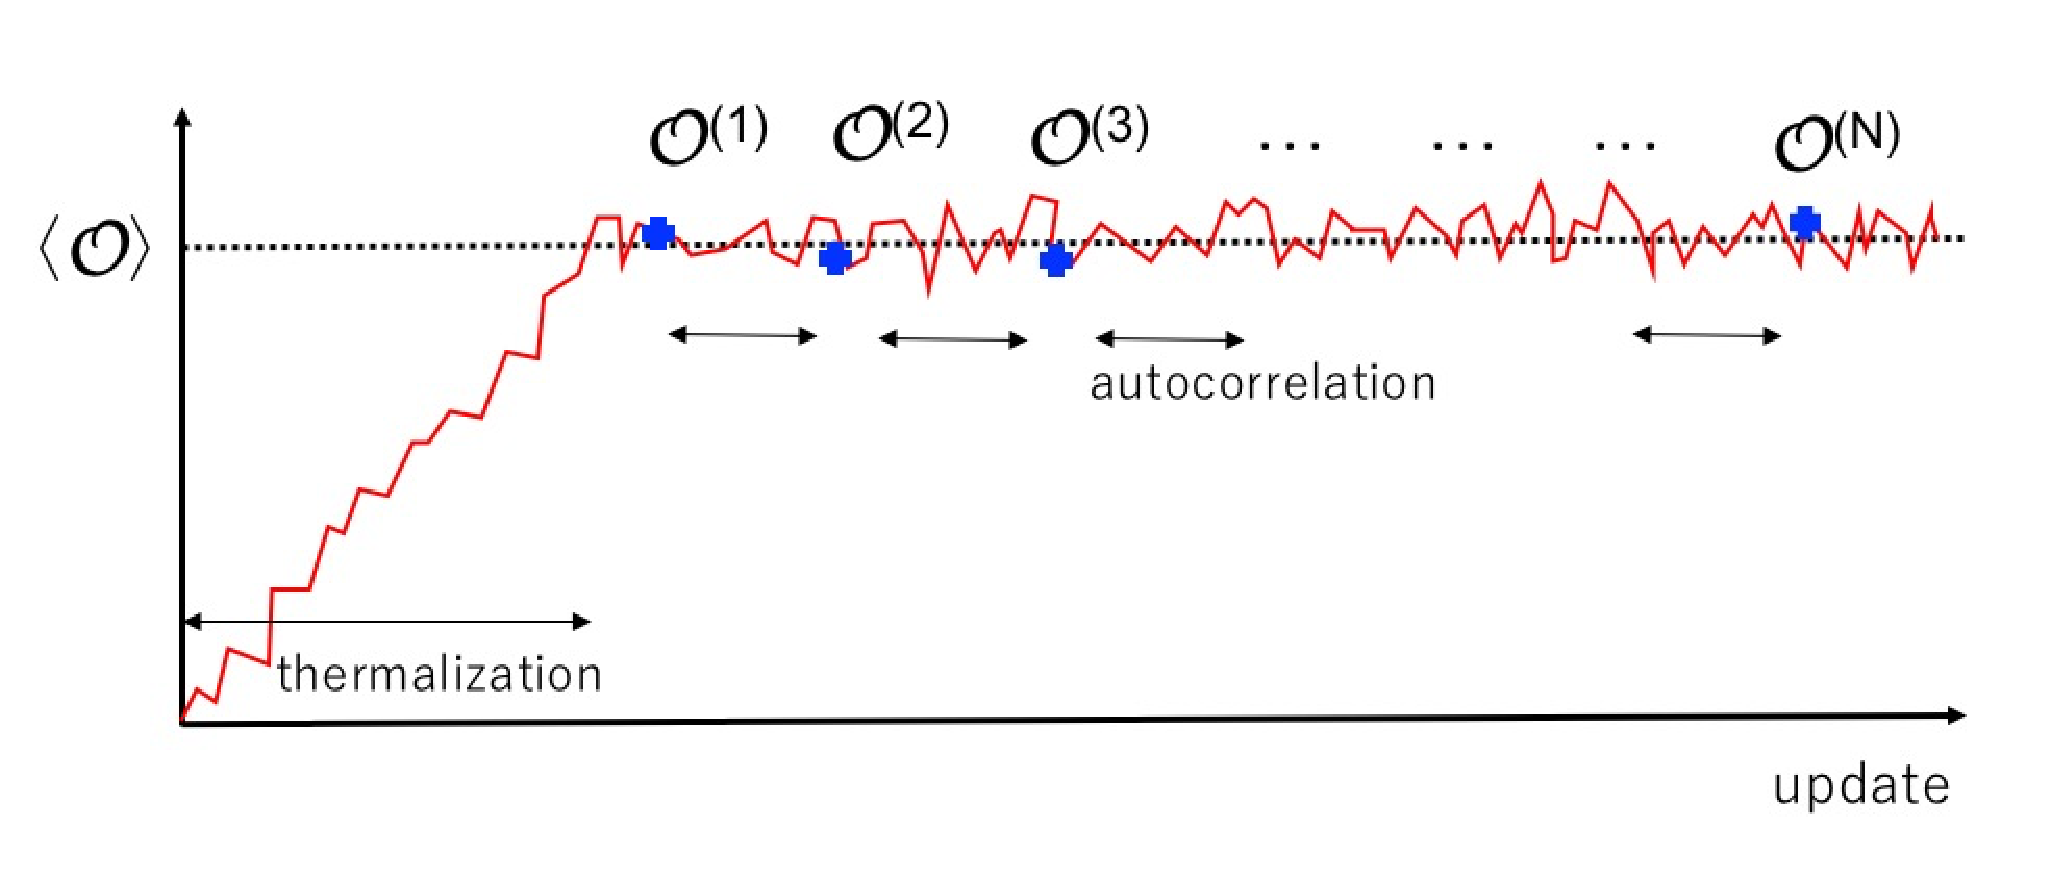
\includegraphics[scale=0.37]{Chapter3-figures/auto.eps} 
 \end{center}
\caption{Schematic illustration on the behavior of ${\cal O}$ under successive update starting from
certain initial configuration. Blue crosses correspond to ${\cal O}^{(n)}$ to be used for the actual average in
Eq.(\ref{eq:5.obs-average}).}
\label{fig:auto}
\end{figure}
%%%%%%%%%%%%%%%%%%%%%%%%%%%%%%
    
    
    
%===============================
\subsection{Hybrid Monte Carlo (HMC)}
%===============================

 Most widely used method   for 
  generating configurations in LQCD 
  is  the hybrid Monte Carlo (HMC) method \cite{Duane:1987de} and its variations.
 The basic procedure of the HMC can be summarized as follows:
 First, we rewrite the partition function by introducing a conjugate momentum field $\pi$,
 so that ${\cal Z}$ is transformed to a phase space functional integral,
\beq
{\cal Z}= \int [d\phi]\ e^{-S(\phi)}= \int [d\Phi] \  e^{- H(\Phi)}, \ \  \ \ \ 
H(\Phi) = \frac{1}{2} \pi^2 + S(\phi) ,
\eeq
where $\Phi\equiv(\phi,\pi)$ and $[d\Phi]\equiv [d\phi d\pi]$.
Then we follow the steps below:
 \begin{enumerate}
 \item[1.]   Start with arbitrary chosen initial configuration, $\phi$.
 \item[2.]  Generate $\pi$ with the Gaussian distribution, 
 \beq 
 P_{\rm G}(\pi) \propto \exp(-\pi^2/2).
 \eeq
\item[3.]  Evolve $\Phi $ under transition probability $P_{\rm H}$ with the {\it reversibility condition}, 
\beq
\label{eq:reversible}
P_{\rm H}(\Phi \rightarrow \Phi') = P_{\rm H}(\Phi'_r \rightarrow \Phi_r),   \ \ \  \Phi_r \equiv (\phi,-\pi). 
\eeq
\item[4.] Accept the configuration $\Phi'$ with the probability, 
\beq 
\label{eq:MET-test}
P_{\rm A} (\Phi \rightarrow \Phi')  = {\rm min.} \{ 1, e^{-\Delta H} \} ,
\eeq
where  $\Delta H=H(\Phi')- H(\Phi)$.  This is called the {\it Metropolis test}  \cite{Metropolis_1953}.
\item[5.] If the new configuration $\Phi'$ is accepted, go to Step 2 with $\phi'$.
 Otherwise, keep the original $\phi$ and go to Step 2. 
\end{enumerate}

The above procedure satisfies the detailed balance  Eq.(\ref{eq:5.det-balance}) 
with $W_{\rm eq}[\phi]=\exp(-S(\phi))$. 
In fact, the Step 4  satisfies the detail balance in phase space (Exercise \ref{prob:10}),
\beq
\label{eq:DT-balance}
e^{-H(\Phi)} P_{\rm A} (\Phi\rightarrow \Phi') = e^{-H(\Phi')} P_{\rm A} (\Phi' \rightarrow \Phi) .
\eeq
Then, we have
\beq
e^{-S(\phi)} P (\phi \rightarrow \phi' ) 
&=& e^{-S(\phi)} \int [d\pi d\pi'] P_{\rm G}(\pi)  P_{\rm H}(\Phi \rightarrow \Phi') P_{\rm A} (\Phi \rightarrow \Phi') , \nonumber \\
&=& \int [d\pi d\pi']\ e^{-H(\Phi)}  P_{\rm H}(\Phi \rightarrow \Phi') P_{\rm A} (\Phi \rightarrow \Phi') ,\nonumber \\
&=& \int [d\pi d\pi']\ e^{-H(\Phi')}  P_{\rm H}(\Phi \rightarrow \Phi') P_{\rm A} (\Phi' \rightarrow \Phi) ,\nonumber \\
&=& \int [d\pi d\pi']\ e^{-H(\Phi')}  P_{\rm H}(\Phi'_r \rightarrow \Phi_r)  P_{\rm A} (\Phi' \rightarrow \Phi) ,\nonumber \\
&=& \int [d\pi d\pi']\ e^{-H(\Phi')}  P_{\rm H}(\Phi' \rightarrow \Phi ) P_{\rm A} (\Phi' \rightarrow \Phi) ,\nonumber \\
&=& e^{-S(\phi')} \int [d\pi d\pi'] P_{\rm G}(\pi')  P_{\rm H}(\Phi' \rightarrow \Phi)  P_{\rm A} (\Phi' \rightarrow \Phi) 
= e^{-S(\phi')}  P (\phi' \rightarrow \phi ) ,
\eeq
where we have used Eq.(\ref{eq:reversible}) to obtain the 4th line, and also used $H(\Phi)=H(\Phi_r)$ 
 to obtain the 5th line. 

Note that $P_{\rm H}$ can be chosen to be any transition probability as long as it satisfies
Eq.(\ref{eq:reversible}).  In practice, the deterministic procedure based on the Molecular Dynamics (MD) 
evolution along the  ``computer"  time $s$ is useful:
\beq
\label{eq:MD}
\frac{d}{ds} 
\left(
\begin{array}{cc}
 \phi  \\
  \pi 
\end{array}
\right)
=
\left(
\begin{array}{cc}
 0 &  1   \\
 -1  & 0   
\end{array}
\right)
\left(
\begin{array}{cc}
  {\delta H (\phi,\pi)}/{\delta \phi}   \\
  {\delta H (\phi,\pi)}/{\delta \pi}
\end{array}
\right) =
\left(
\begin{array}{cc}
 \pi  \\
  -  {\delta S (\phi)}/{\delta \phi}
\end{array}
\right) ,
\eeq
which leads to
\beq
P_{\rm H}(\Phi \rightarrow \Phi')  = \delta (\Phi' - \Phi(s)),
\eeq
 on the phase space trajectories, $\Phi = \Phi(0) \rightarrow \Phi(s)$. 
 
If we do not introduce the MD before the Metropolis test $P_{\rm A}$,
the procedure is essentially the MCMC with the Metropolis test.  It
becomes, however, very slow for non-local action such as
Eq.(\ref{eq:Seff}) where $S_{\rm G}(U)$ is local in spacetime while
${\rm Ln Det} F(U)$ is non-local.  The MD is a nice way to evolve the
whole variables on the lattice at once.  The computer time $s$ needs
to be discretized with a step size $\varepsilon$, which brings
inevitable numerical error in MD. However, the Metropolis test in Step
4 eliminates such error so that no extrapolation to $\epsilon=0$ is
required in HMC.

 There are numerical algorithms in MD to satisfy the reversibility and
 preserve the phase space area exactly for finite $\varepsilon$.  The
 {\it leapfrog integrator} is one of such algorithms widely used in
 LQCD (see Appendix [Leapfrog integrator in molecular dynamics]).
 Since this conserves the Hamiltonian with $0(\varepsilon^2$)
 accuracy, the acceptance rate in Step 4 can be kept high.


 In LQCD simulations, we need to treat the unitary matrices $U_{\mu}(n)$ as dynamical variables, i.e.
  the MD should be performed on the SU($N_c$)  group manifold.
 The appropriate choice of the conjugate momentum would be the element of the Lie algebra,
  $ P_l =  R_l^a t^a = -i  (d{U_l}/ds) U_l^{-1} $ (see Eq.(\ref{eq:LR-form})) where
  we have abbreviated the link index $n$ and site index $\mu$  as $l$ for simplicity.
 This  leads to the
  equation of motion for $U_l$,
\beq
\label{eq:EOM-U}
\frac{d U_l}{ds}= i P_l U_l .  
\eeq
The effective Hamiltonian is naturally written as 
\beq
\label{eq:EOM-H}
H= {\rm tr} \sum_{l} P_l^2 + S_{\rm eff}(U) , 
\eeq
 where ${\rm tr}$ is over color indices with the normalization given in Eq.(\ref{eq:tt}).
 Then the  time-parameter independence  $\frac{dH}{ds}=0$ leads to the equation of motion for $P_l$
 (Exercise \ref{prob:11}),
  \beq
 \label{eq:EOM-P} 
 \frac{dP_l}{ds} = - i  \sum_{i,j} t^a \left( t^a U_l \right)_{ij} \frac{\partial S_{\rm eff}(U)}{\partial (U_l)_{ij}}.
\eeq
In the actual simulations, the ${\rm ln Det}F(U) $ part of the effective action is treated by
introducing a set of bosonic variables (pseudofermions) through the identity,
\beq
{\rm Det} F = ({\rm Det} F^{-1})^{-1} = \int [d\chi^* d\chi] \ \exp \left( -\sum_{IJ} \chi^*_{I} F_{IJ}^{-1} \chi_J \right),
\eeq
where $I$ and $J$ stand for all possible internal and spacetime indices carried by $F$.    
For further details of HMC (and its variations) with pseudofermions, 
consult the recent review \cite{Schaefer:2012tq} and references therein.


%===========================
\subsection{Error estimate}
%===========================

There are two kinds of errors  in the data obtained from  LQCD simulations.\\

\noindent {\bf Systematic errors:} \\
 They are related to the lattice spacing $a$, the lattice volume $L^3$,
  and the quark masses ($m$).  During 
  the continuum extrapolation ($a\rightarrow 0$) and the thermodynamic extrapolation ($L \rightarrow \infty$) 
  under the  guidance of  the asymptotic scaling for small $a$ 
 and the finite size scaling for  large $L$, some systematic errors are brought in.
 Also,  one often needs to make extrapolation to the physical quark mass by using 
 lattice data  with heavier  quark masses. This  also brings some
 systematic errors.\\
 
 \noindent
{\bf Statistical error:} \\
It originates from the importance sampling.  A very useful procedure to estimate such error
 commonly used in LQCD is the {\it jackknife resampling method}. (The name
  originates from the ``jackknife"  which is an easy and  portable  tool  for general purposes).
  Let us consider the mean and the unbiased variance of a certain quantity $ {\cal O}$,
  \beq
   \langle {\cal O} \rangle = \frac{1}{N} \sum_{n=1}^N {\cal O}^{(n)}  \pm \sqrt{\frac{\sigma^2({\cal O} )}{N}}, \ \ \ \
   \sigma^2({\cal O}) = \left( \frac{N}{N-1} \right)  \frac{1}{N} \sum_{n=1}^N ( {\cal O}^{(n)}  - \langle {\cal O} \rangle )^2,
  \eeq
where the factor $\frac{N}{N-1}$ is called the Bessel's correction.
 The jackknife samples are obtained by
 \beq
  {\cal O}^{(n)}_J= \frac{1}{N-1} \sum_{n' \neq n}  {\cal O}^{(n')}      \ \ \ \  (n=1, \cdots, N).
 \eeq
 If we need to make a quick estimate of the 
  mean and the variance of a function $f({\cal O})$, we have
 \beq
\label{eq:jack}
 \langle f({\cal O}_J)\rangle = \frac{1}{N} \sum_{n=1}^{N} f( {\cal O}^{(n)}_J) \pm  \sqrt{\frac{\sigma_J^2(f)}{N}}, \ \ \ \ 
  \sigma_J^2(f) = (N-1) \sum_{n=1}^N ( f( {\cal O}^{(n)}_J) -  \langle f( {\cal O}_J)\rangle)^2. 
\eeq
For $f( {\cal O})={\cal O}$, we recover the original  mean and variance;
 $\langle  {\cal O}_J \rangle = \langle  {\cal O} \rangle$ and  $\sigma_J^2({\cal O})=\sigma^2({\cal O})$. (Exercise \ref{prob:12}).
One can generalize this procedure by dividing $N$ into $N_b=N/n_b$  
with the bin-size $n_b$ and create the $N_b$ jackknife samples. 
 Eq.(\ref{eq:jack})  corresponds to the case with $n_b=1$.

 
 
%===========================
\subsection{Heavy quark potential}
%===========================

 As one of the examples of the accurate  inter-quark potential obtained from LQCD simulations,
 we  show in Fig.\ref{fig:QQbar-pot}  the  
 dimensionless ${\rm Q}\bar{\rm Q}$ potential 
$[V(R)-V(R_0)]\times R_0$
 as a function of $R/R_0$ extracted from the calculation of the   
   Wilson loop in the quenched approximation.
 $R$ is a distance between the heavy quarks
  and $R_0$ is called the {\it Sommer scale}   defined by
 $  \left. R^2 \frac{dV(R)}{dR} \right|_{R=R_0}=1.65$.
 
 Simulations with different lattice couplings $6/g^2$
  correspond to different lattice spacings $a$.
 The latter can be fixed, e.g., by   
 taking a phenomenological value
  $R_0\simeq 0.5\ {\rm fm}$. 
    The lattice spacings in the physical uniit in the figure are
   $a=0.094\ {\rm fm}$ (squares: $\beta=6/g^2=6.0$),
    $a= 0.069\ {\rm fm}$ (circles: $\beta=6.2$)
  and  $a=0.051\ {\rm fm}$ (triangles: $\beta=6.4$).
  Since there exists no appreciable $a$ dependence of the potential,
 the system is already close enough to the continuum limit. 
  
 Fig.\ref{fig:QQbar-pot} clearly shows that the 
  heavy quark potential has a linear confining part
   at long distance and an attractive Coulombic part 
    at short distance. The LQCD results agree
     not only qualitatively but also quantitatively  
  with an empirical linear + Coulomb potential
  (the Cornell potential)    shown by the solid line,
   $V(r) = Kr - b/r + {\rm const}$ with $b=0.295$.  
   
% FIG %%%%%%%%%%%%%%%%%%%%%%%%%%   
\begin{figure}[t]
\begin{center}
%\framebox[74mm]{\rule[-26mm]{0mm}{52mm}}
%\includegraphics[scale=0.6]{as-scale.eps}
\includegraphics[scale=0.5]{Chapter3-figures/QQbar-pot.eps} 
 \end{center}
\caption{A dimensionless ${\rm Q}\bar{\rm Q}$ potential as a 
 function of a dimensionless quark$-$anti-quark
 separation $R/R_0$ with $R_0$ being the Sommer scale. 
 Different  symbols correspond to different lattice couplings
  $g(a)$    and hence different lattice spacings. 
  The solid line shows an empirical Cornell potential. 
  The figure is adapted from \cite{Bali:2000gf}.
  }
\label{fig:QQbar-pot}
\end{figure}
%%%%%%%%%%%%%%%%%%%%%%%%%%%%%%


%============================
\subsection{Masses of light hadrons}
%============================

 Meson masses and baryon masses can be calculated with high accuracy
 by LQCD simulations with dynamical quarks.  The starting point is the
 hadronic correlation functions $C_{\rm H=M,B} (n,n')$ in
 Eqs.(\ref{eq:correlation-M},\ref{eq:correlation-B}) integrated over
 the spatial coordinates, $\mathbf{n}$ and
 $\mathbf{n}'$, 
\beq \label{eq:5.D-tau} C_{\rm H}(\tau)
 = \sum_{\mathbf{n}, \mathbf{n}'} C_{\rm H}
 (n,n') \xrightarrow[\tau \rightarrow \infty] \ |Z_{\rm H}|^2 {\rm
 e}^{-M_{\rm H} \tau} , 
\eeq 
where $\tau= (n_4-n_4')a$ is the temporal
 distance between the source at $n'$ and the sink at $n$, and $M_{\rm
 H}$ ($Z_{\rm H}$) corresponds to the mass (the pole residue) of a
 lightest bound state in each channel.  If the temporal extent of the
 lattice is infinite, one can extract the hadron mass from the
 formula, $M_{\rm H}= -(1/\tau) \ln C_{\rm
 H}(\tau)|_{\tau \rightarrow \infty} $.  In practice, the {\it
 effective mass} defined below is more useful, \beq aM_{\rm H}^{\rm
 eff}(\tau) = \ln \left( \frac{C_{\rm H}(\tau)}{C_{\rm H}(\tau+a)
 } \right) .
\eeq
The asymptotic plateau of the effective mass at large $\tau$
     corresponds to the hadron mass.  In actual simulations, the
     temporal extent is limited ($0 \le \tau/a \le N_{\tau}$), so that
     the exponential damping of Eq.(\ref{eq:5.D-tau}) is replaced by
     $C_{\rm H} \rightarrow \exp[-M_{\rm H} \tau ] \pm \exp [-M_{\rm
     H} (N_{\tau} a - \tau)]$ where $+ (-)$ for the periodic
     (anti-periodic) boundary condition.
     
 Shown in the left panel of Fig.\ref{fig:hadron-mass} is the
 dimensionless effective masses ($a M_{\rm H}^{\rm eff}$) against
 $\tau/a=(n_4-n_4')$ \cite{Durr:2008zz}.  Data points are the
 effective masses for the pion $(\pi)$, the kaon $(K)$, the nucleon
 ($N$), the cascade baryon ($\Xi$) and the omega baryon $(\Omega$)
 calculated on the lattice with $a \simeq 0.085$ fm and the pion mass
 $M_{\pi} \simeq 190$ MeV.  Reasonable plateau above $\tau/a > 9$ can
 be seen within the error bars.
 
 Shown in the right panel of Fig.\ref{fig:hadron-mass} is the
 $M_{\pi}^2$-dependence of the $N$ and $\Omega$ masses for three
 different values of $a$ \cite{Durr:2008zz}.  The crosses are the
 values extrapolated to the continuum limit and to the physical pion
 mass.  The $N$ and $\Omega$ masses predicted from LQCD and
 corresponding experimental numbers are
\beq
\label{eq:mass-LQCD}
M_N^{\rm LQCD} &=& 0.936(25)(22) \ {\rm GeV}, \ \ \ M_\Omega^{\rm
LQCD} =1.676(20)(15)\ {\rm GeV}, \\ M_N^{\rm exp.} &=& 0.939 \ {\rm
GeV}, \ \ \ \ \ \ \ \ \ \ \ \ \ \ \ \ M_\Omega^{\rm exp.} =1.672 \
{\rm GeV}.
\eeq
  Note that the numbers in the first (second) parenthesis in
 Eq.(\ref{eq:mass-LQCD}) represent the statistical (systematic) errors
 on the last digits.

% FIG %%%%%%%%%%%%%%%%%%%%%%%%%%   
\begin{figure}[t]
\begin{center}
%\framebox[74mm]{\rule[-26mm]{0mm}{52mm}}
%\includegraphics[scale=0.6]{as-scale.eps}
\includegraphics[scale=0.29]{Chapter3-figures/effective-mass.eps} \ \ 
\includegraphics[scale=0.28]{Chapter3-figures/NO_scaling.eps}
 \end{center}
\caption{(Left) The effective masses of hadrons against the 
 temporal separation between the source and the sink. 
(Right)  Hadron masses under the changes of the (pion mass)$^2$ as well as the lattice spacing $a$.
The figures are taken from \cite{Durr:2008zz}
  }
\label{fig:hadron-mass}
\end{figure}
%%%%%%%%%%%%%%%%%%%%%%%%%%%%%%%

Shown in Fig.\ref{fig:pn-mass} are the high precision numerical
 results of the hadron mass splittings obtained by the QCD+QED lattice
 simulations with dynamical $u,d,s,c$ quarks \cite{Borsanyi:2014jba}.
 The horizontal lines are the experimental values and the grey shaded
 regions represent the experimental errors.  Red dots are the lattice
 results with their uncertainties denoted by the vertical error bars.
 The neutron-proton mass differences from numerical simulations and
 the corresponding experimental numbers are
\beq
(M_n-M_p)^{\rm LQCD+QED} &=&\Delta N = 1.51(16)(23)\   {\rm MeV}, \\
(M_n-M_p)^{\rm exp.} &=& 1.29\   {\rm MeV}. 
\eeq

% FIG %%%%%%%%%%%%%%%%%%%%%%%%%%
\begin{figure}[t]
\begin{center}
%\framebox[74mm]{\rule[-26mm]{0mm}{52mm}}
%\includegraphics[scale=0.6]{as-scale.eps}
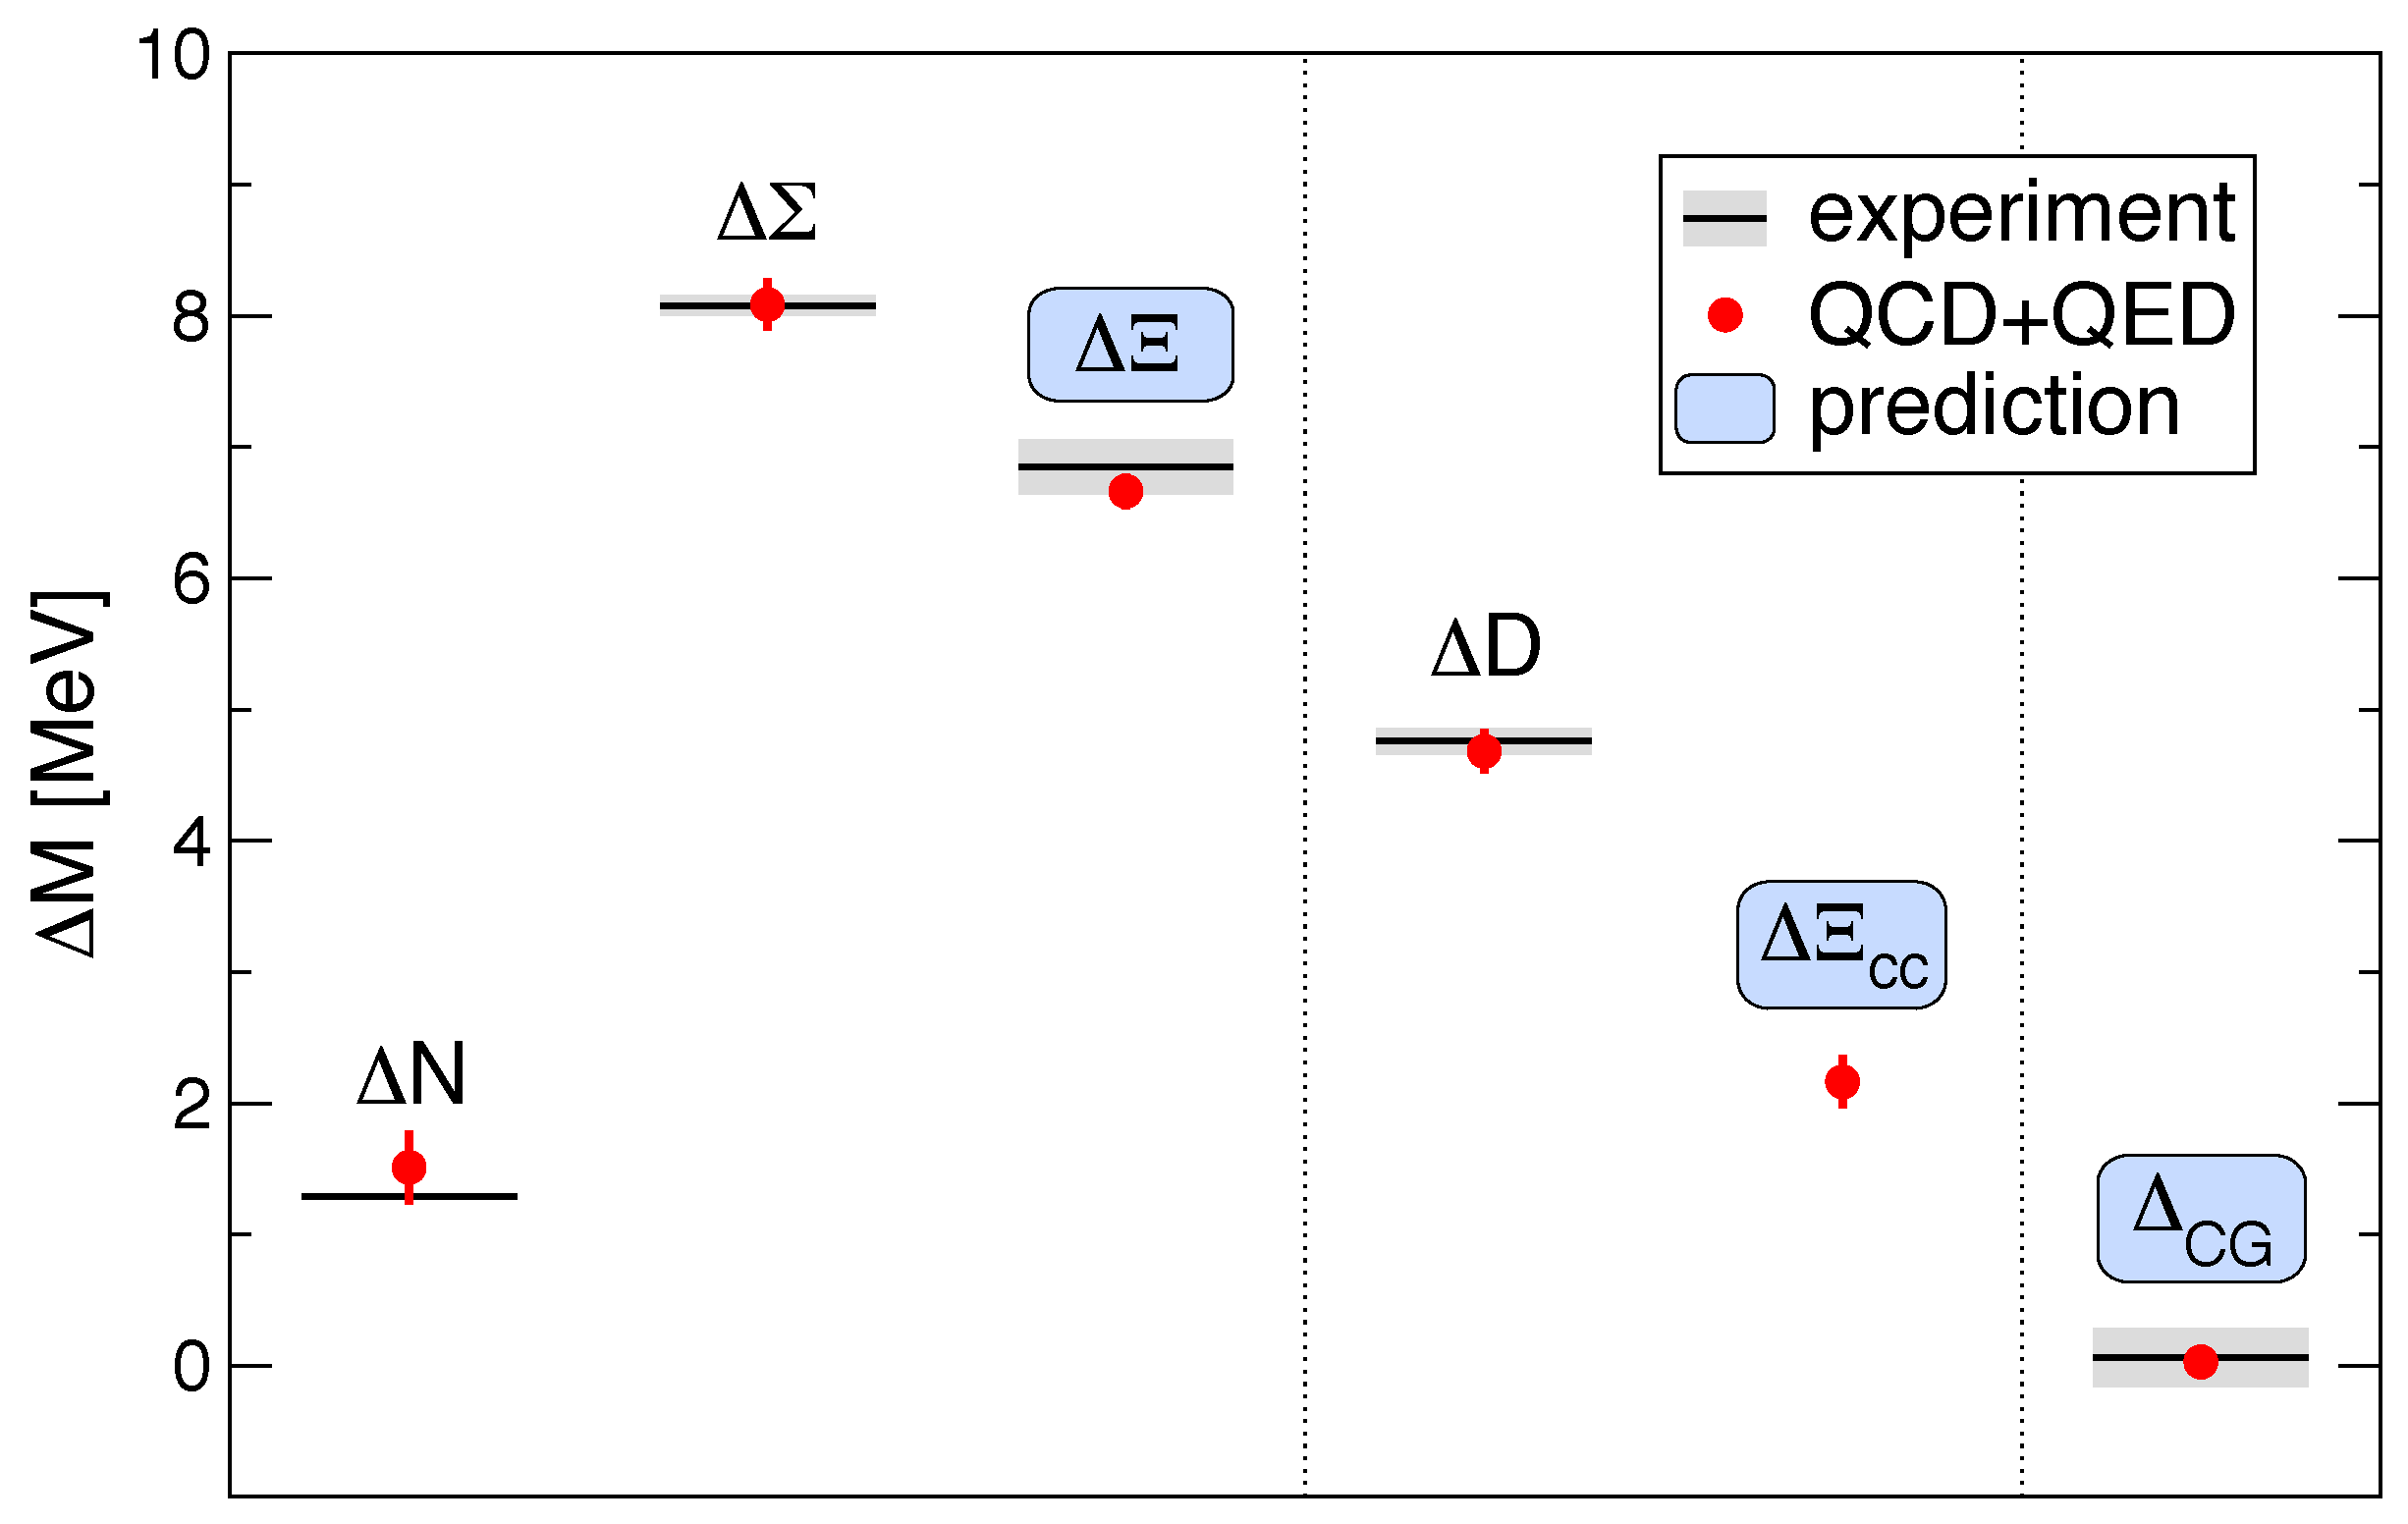
\includegraphics[scale=0.2]{Chapter3-figures/pn-mass.eps}
 \end{center}
\caption{Mass splittings in channels that are stable under the strong and electromagnetic interactions.
$\Delta N=M_n-M_p$, $\Delta \Sigma = M_{\Sigma^-}- M_{\Sigma^+}$,
$\Delta \Xi =M_{\Xi^-}- M_{\Xi^+}$,
$\Delta D= M_{D^{\pm}} - M_{D^0}$,
$\Delta \Xi_{cc} = \Delta \Xi_{cc}^{++} - \Delta \Xi_{cc}^{+}$,
$\Delta CG = \Delta N-\Delta \Sigma + \Delta \Xi$.
The figure is taken from
\cite{Borsanyi:2014jba}.
  }
\label{fig:pn-mass}
\end{figure}
%%%%%%%%%%%%%%%%%%%%%%%%%%%

Since all hadrons are composite particles of quarks and gluons, there
are numerous excited states \cite{RPP}.  To extract the properties of
the excited hadrons from LQCD, only looking at the asymptotic form as
shown in Eq.(\ref{eq:5.D-tau}) is not sufficient, and more
sophisticated methods such as the maximal entropy method (MEM) and the
variational method are required.  Interested readers should consult
the reviews \cite{Asakawa:2000tr,Fodor:2012gf} and references there
in.


%%%%%%%%%%%%%%%%%%%%%%%%
\section{Lattice QCD and nuclear force}
%%%%%%%%%%%%%%%%%%%%%%%%

Understanding of the nuclear force from QCD is one of the most
 challenging problems in nuclear physics.  Below the pion production
 threshold, the notion of the $NN$ potential (either in the coordinate
 space or in the momentum space) has been known to be useful, since it
 can be used not only to describe the two-body system but also to
 study nuclear many-body problems through ab-initio
 calculations \cite{this_book}.

  Several high precision phenomenological $NN$ forces have been
  constructed to reproduce the neutron-proton and proton-proton
  scattering data (about 4500 data points) with a $\chi^2/{\rm
  dof} \sim 1$. However, they have typically 20-40 fitting parameters:
  e.g. the CD Bonn potential, AV18 potential and N$^3$LO chiral
  effective field theory have 38, 40, and 24 parameters,
  respectively \cite{Machleidt:2007ms}.  If one tries to extend these
  to hyperon-nucleon and hyperon-hyperon interactions, the task
  becomes extremely tough since the number of parameters increases and
  the scattering data are scarce.
 
  Under this situation, it is highly desirable to study
  baryon-baryon interactions from first principle LQCD simulations,
  where all the hadronic interactions are controlled only by the QCD
  coupling $g$ and the quark mass $m$ whose values are pretty well
  determined at present by the precision QCD
  simulations \cite{Aoki:2013ldr}.
 
 The finite volume method (FVM), a theoretical framework to study
  hadron-hadron interactions from LQCD, was first proposed by
  L\"{u}scher \cite{luescher}: For two hadrons in a finite box with a
  spatial size $L^3$, an exact relation between the energy spectra in
  the box and the elastic scattering phase shift can be derived.  If
  the range of the hadronic interaction $R_{\rm QCD}$ is sufficiently
  smaller than the size of the box $R_{\rm QCD}<L/2$, the behavior of
  the the equal-time Bethe-Salpeter amplitude (or more precisely the
  Nambu-Bethe-Salpeter (NBS) amplitude) $\psi (\mathbf{r})$ in the
  interval $R_{\rm QCD} < | \mathbf{r} | < L/2 $ has sufficient
  information to relate the phase shift and the energy shift 
$\Delta E=M_{\rm HH}-2M_{\rm H}$.
  
The HAL QCD method was proposed as another theoretical framework to
 study the hadron-hadron interactions from LQCD by Ishii, Aoki and
 Hatsuda \cite{Ishii:2006ec} and was further developed by HAL QCD
 Collaboration \cite{HALQCD:2012aa}.  The starting point is the same
 equal-time NBS amplitude $\psi (\mathbf{r})$: Instead of looking at
 the amplitude outside the range of the interaction, the internal
 region $ |\mathbf{r} | < R_{\rm QCD}$ is considered and an
 energy-independent non-local potential $U(\mathbf{r}, \mathbf{r}')$
 is deduced from $\psi (\mathbf{r})$.  Since
 $U(\mathbf{r}, \mathbf{r}')$ in QCD is spatially localized due to the
 confinement of quarks and gluons, it is affected only weakly by the
 finite lattice volume. Physical quantities such as the scattering
 phase shifts, bound state spectra, and resonance energies can be
 calculated by solving the integro-differential differential equation
 satisfied by $\psi (\mathbf{r})$ with $U(\mathbf{r}, \mathbf{r}')$.
   
  Recently, a detailed comparison between the FVM and the HAL QCD
  method has been carried out: Although they agree with each other
  quite accurately for non-resonant pion-pion scattering, large signal
  to noise ratio inherent in the effective mass $\Delta E^{\rm
  eff}(\tau)$ for baryon-baryon scatterings prevents FVM to extract
  scattering observables \cite{Iritani:2015dhu}.  Therefore, we will
  focus on the HAL QCD method below.
  
%=============================================     
\subsection{Master equation for baryon-baryon interaction}
%=============================================  
  
Let us consider the baryon-baryon correlation in
Fig.\ref{fig:correlation}(c) and define the equal-time NBS amplitude
$\psi_{\ell}(\mathbf{r},\tau)$ from its large $\tau$ behavior: 
\beq
C_{\rm BB}(\mathbf{r}, \tau)
=\sum_{\mathbf{n}',\mathbf{m}'} \left. C_{\rm
BB}(n,m,n',m') \right|_{n_4=m_4,n_4'=m_4'} \rightarrow \sum_{\ell}
a_{\ell} \psi_{\ell} (\mathbf{r},\tau) e^{-E_{\ell} \tau} , 
\eeq 
where
$\mathbf{r}=(\mathbf{n}-\mathbf{m}) a$, $\tau=(n_4-n_4')a$, and
$\psi_{\ell} (\mathbf{r},\tau)$ being the NBS wave function for
$\ell$-th scattering state on the lattice.  For large lattice size,
$E_{\ell}$ is very dense, so that it is impossible to identify each
level.  This causes a fatal problem in FVM as mentioned above.  On the
other hand, if we define $ C_{\rm BB}(\mathbf{r};\tau)= {\cal
R}(\mathbf{r},\tau) e^{-2M_{\rm B} \tau}$, the following
integro-differential equation can be derived below the inelastic
threshold ($\tau > M_{\pi}^{-1}$),
\beq
  \left\{
  \frac1{4M_{\rm B}}\frac{\partial^2}{\partial \tau^2} 
  -\frac{\partial}{\partial \tau}
  - H_0
  \right\}
  {\cal R}(\mathbf{r},\tau)
  =
  \int d^3 r'
  U(\mathbf{r}, \mathbf{r}')
  {\cal R}(\mathbf{r}', \tau),
  \label{eq.tdep}
\eeq
 with  $H_0= - \nabla^2/M_{\rm B}$.
 This is the master equation which has the 
correct information of the S-matrix and hence the scattering phase shift for
elastic $BB$ scatterings \cite{HALQCD:2012aa}.
  
  If we further focus on the 
  energies  much below  the inelastic threshold,
   the velocity expansion
   of $U(\mathbf{r},\mathbf{r}')$ in terms of its  non-locality can be adopted.
   In fact, the potential with hermiticity, 
   rotational invariance, parity symmetry,   and time-reversal invariance may be expanded as \cite{okubo}
\begin{eqnarray} 
\label{eq:U-del}
  U(\mathbf{r},\mathbf{r}')    &=& V(\mathbf{r}, \mathbf{v}) \delta(\mathbf{r}-\mathbf{r}'), \\
 V(\mathbf{r}, \mathbf{v})    & =&
   \underbrace{V_{\rm C}(r) + V_{\rm T}(r) S_{12}}_{\rm LO} 
  + \underbrace{V_{\rm LS}(r) {\mathbf{L}} \cdot {\mathbf{S}}}_{\rm NLO}  
  +\underbrace{{O}(\mathbf{v}^2)}_{{\rm N}^2{\rm LO}}
  + \cdots , 
   \label{eq:V-pot}
\end{eqnarray} 
   where $\mathbf{v} = \mathbf{p}/(M_{\rm B}/2) $, $\mathbf{L} = \mathbf{r} \times \mathbf{p} $, 
   $\mathbf{p} = -i \nabla$ and 
   $S_{12}=3(\mathbf{\sigma}_1 \cdot \mathbf{r})(\mathbf{\sigma}_2 \cdot \mathbf{r})/r^2 - \mathbf{\sigma}_1 \cdot \mathbf{\sigma}_2$.
     The central potential $V_{\rm C}$ and 
  the tensor potential $V_{\rm T}$ are classified as
  the leading order (LO) potentials since they
  are of $O(\mathbf{v}^0)$. The next-to-leading (NLO) potential of  
  $O(\mathbf{v})$ is the spin-orbit potential  $V_{\rm LS}(r)$. 

%=============================================
\subsection{Baryon-baryon interaction in flavor SU(3) limit}
%=============================================  
  
 % FIG %%%%%%%%%%%%%%%%%%%%%%%%%%
\begin{figure}[t]
\begin{center}
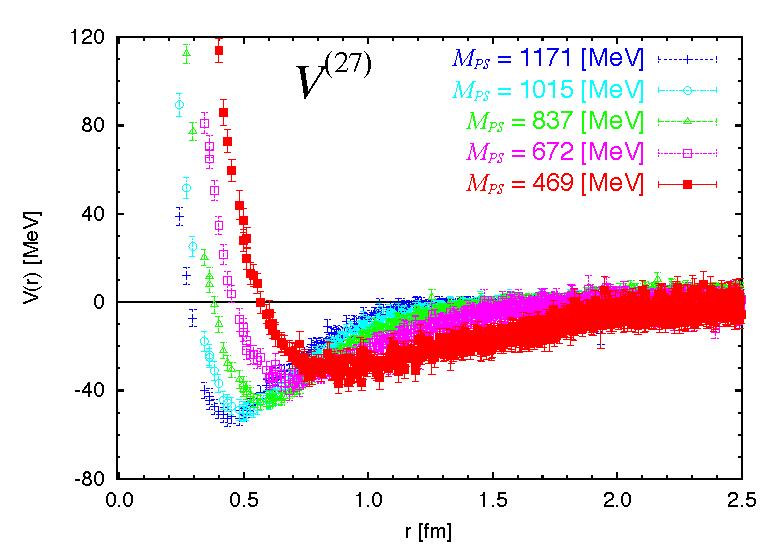
\includegraphics[scale=0.55]{Chapter3-figures/Vc_27_npa2.eps}\ \ \ \ \ \ \ 
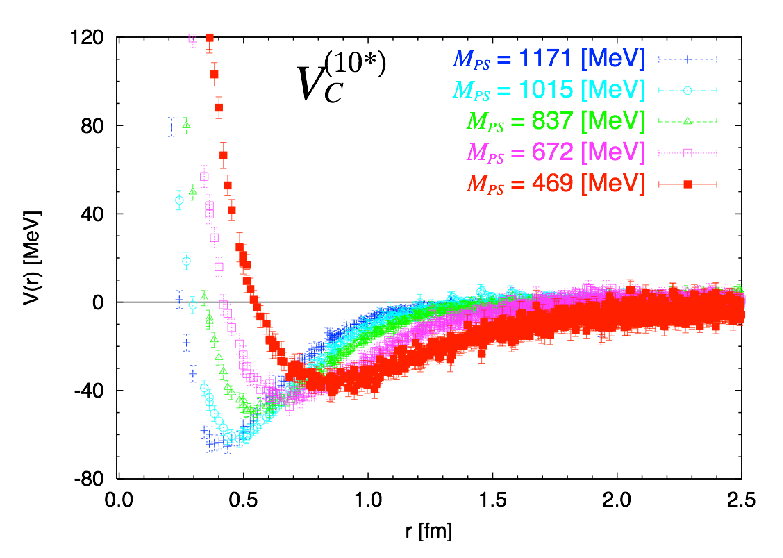
\includegraphics[scale=0.55]{Chapter3-figures/Vc_10s_npa2.eps}\\
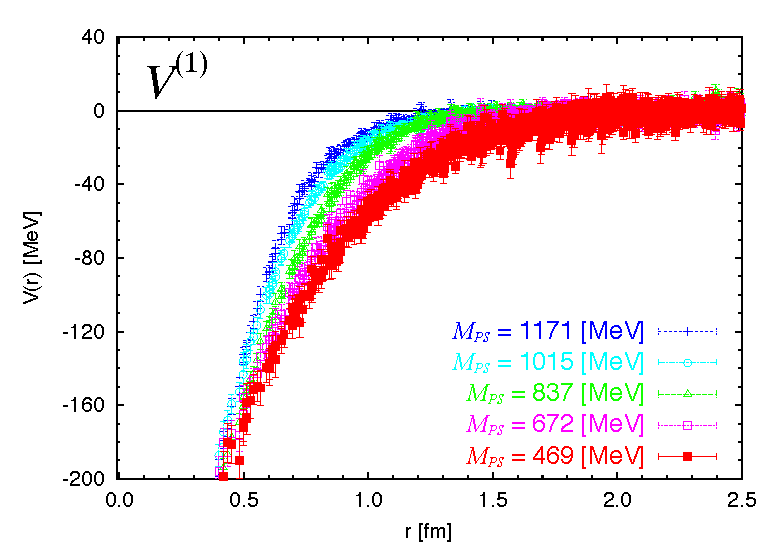
\includegraphics[scale=0.55]{Chapter3-figures/Vc_1_npa2.eps}\ \ \ \ \ \ \ 
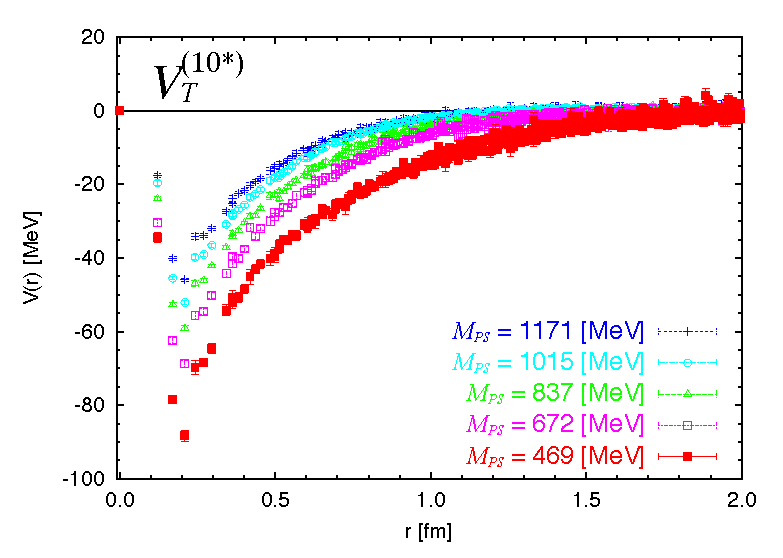
\includegraphics[scale=0.55]{Chapter3-figures/Vt_10s_npa2.eps}
 \end{center}
\caption{The baryon-baryon potentials from LQCD simulations in the flavour
SU(3) limit with several different masses of pseudo-scalar meson. 
The figures are taken from \cite{Inoue:2011ai}.
  }
\label{fig:NN-potential}
\end{figure}
%%%%%%%%%%%%%%%%%%%%%%%%%%%%%
  
 To obtain qualitative understandings of the nuclear force from QCD,
  the $S$-wave interaction between octet baryons  
 in the flavour SU(3) limit  would be a good starting point.
 In this case,  two baryon states with a given angular momentum
are labelled by the irreducible flavour multiplets,
\begin{equation}
 {\bf 8} \otimes {\bf 8} 
 = \underbrace{{\bf 27} \oplus {\bf 8}_s \oplus {\bf 1}}_{\mbox{symmetric}} ~ 
  \oplus \underbrace{{\bf 10}^* \oplus {\bf 10} \oplus {\bf 8}_a}_{\mbox{anti-symmetric}} \ . 
\end{equation}
Here ``symmetric" and ``anti-symmetric" stand for the symmetry under the
flavour exchange of two baryons.
For the system in the orbital S-wave, the Pauli principle between two baryons imposes 
${\bf 27}$, ${\bf 8}_s$ and ${\bf 1}$ to be spin singlet  ($^1S_0$) while 
${\bf 10}^*$, ${\bf 10}$ and ${\bf 8}_a$ to be spin triplet ($^3S_1$). 
Since there are no mixings among different multiplets in the SU(3) limit, 
one may define the corresponding potentials as
 \beq
^1S_0 \ &:& \  V^{({\bf 27})}(r), \ V^{({\bf 8}_s)}(r), \ V^{({\bf 1})}(r), 
\\ 
^3S_1 \ &:& \ V^{({\bf 10}^*)}(r), \ V^{({\bf 10})}(r), \ V^{({\bf 8}_a)}(r) ~.
\eeq
The diagonal potential ($B_1B_2 \rightarrow B_1 B_2)$ and  
 the off-diagonal potentials ($B_1B_2 \rightarrow B_3 B_4$) in the particle basis, 
 are obtained by  suitable combinations
of $V^{(\alpha)}(r)$ with $\alpha={\bf 27},{\bf 8}_s,{\bf 1},{\bf10}^*,{\bf 10},{\bf 8}_a$.

% FIG %%%%%%%%%%%%%%%%%%%%%%%%%%
\begin{figure}[t]
\begin{center}
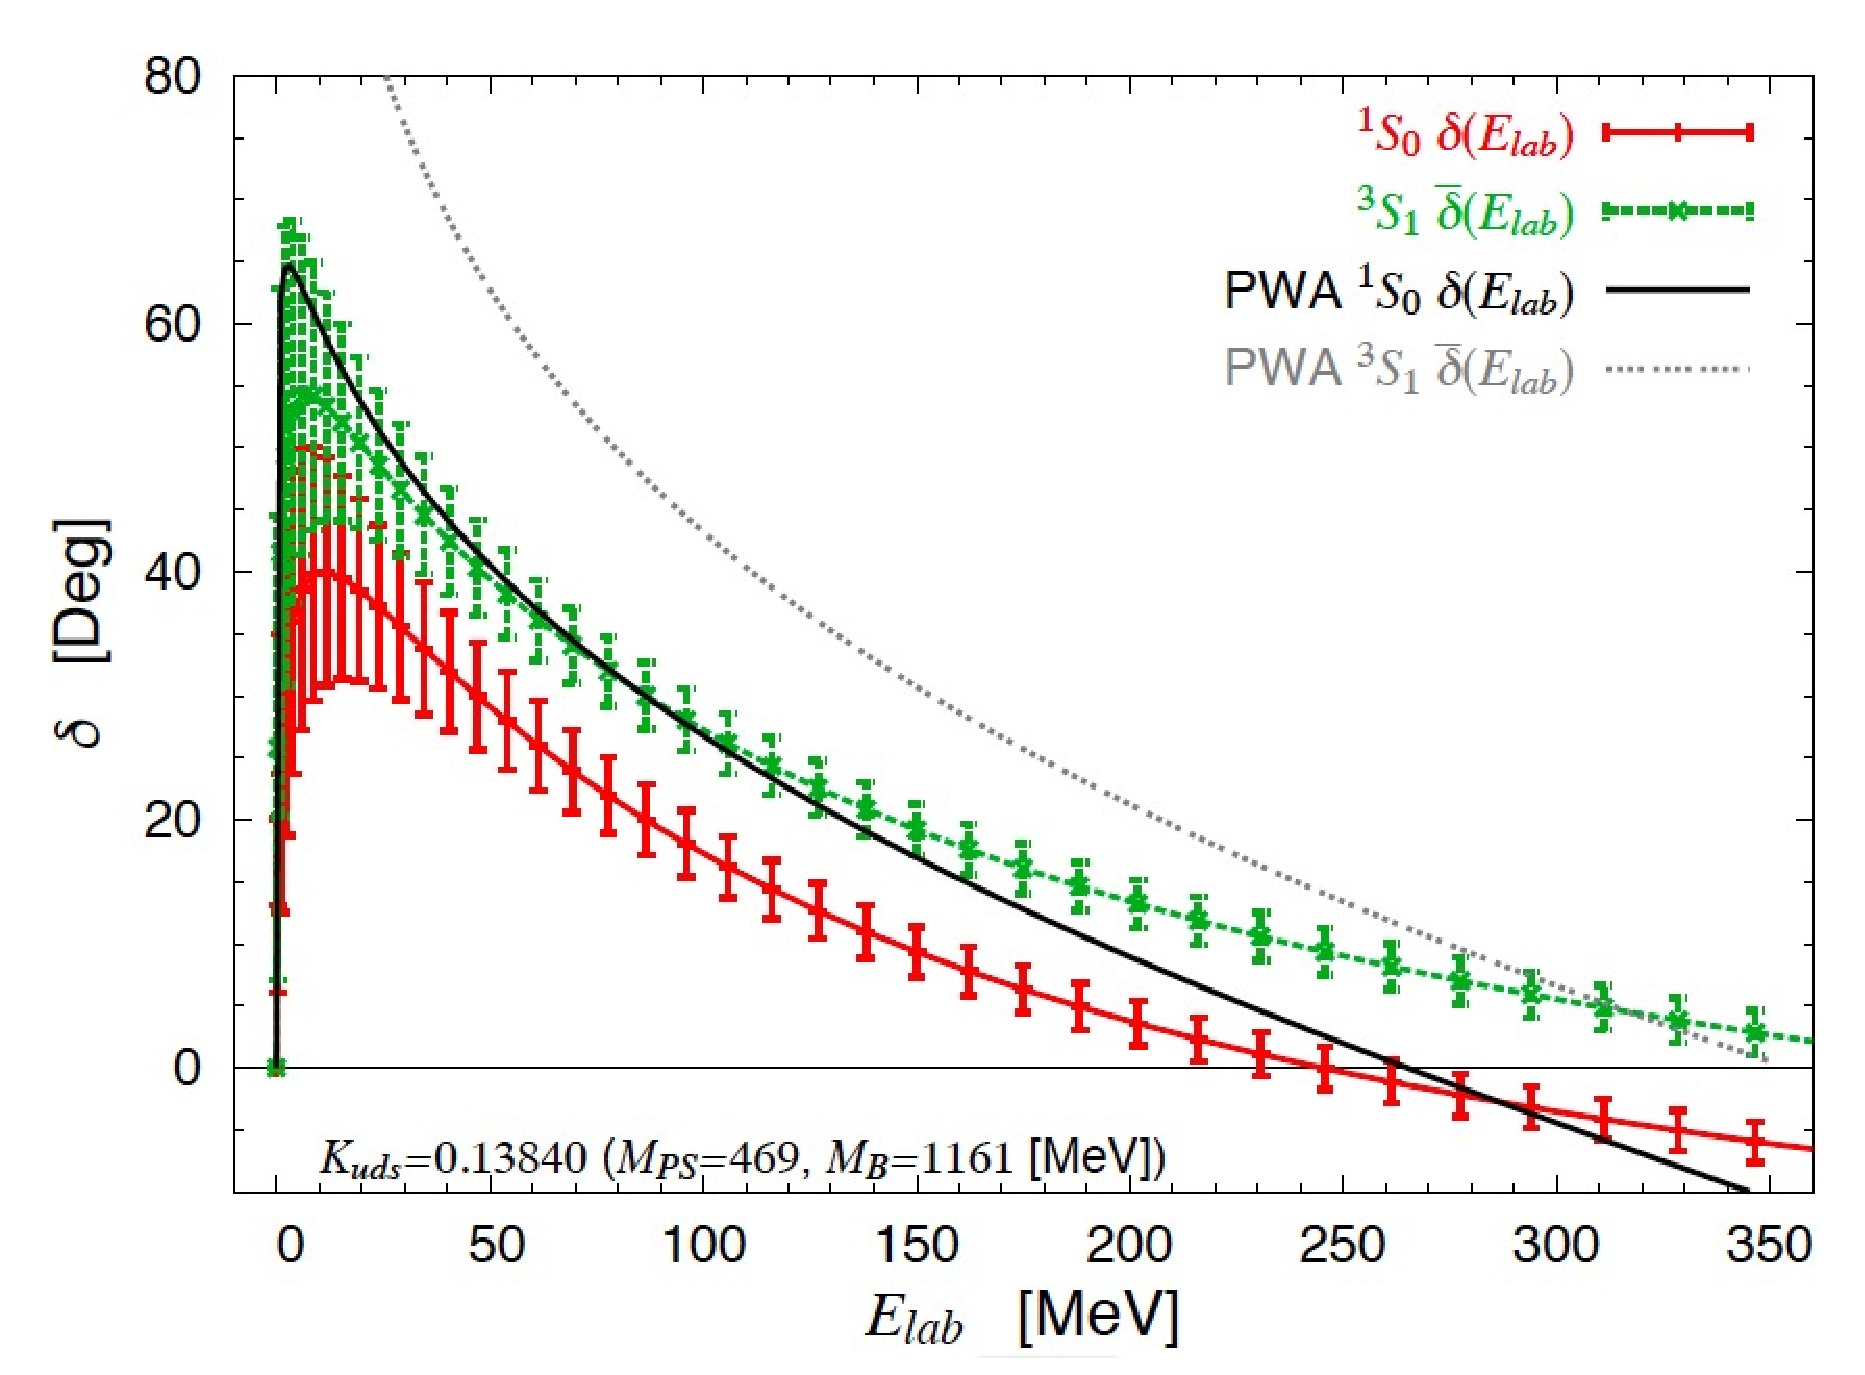
\includegraphics[scale=0.25]{Chapter3-figures/phase-shift.eps}\ \ \ \ 
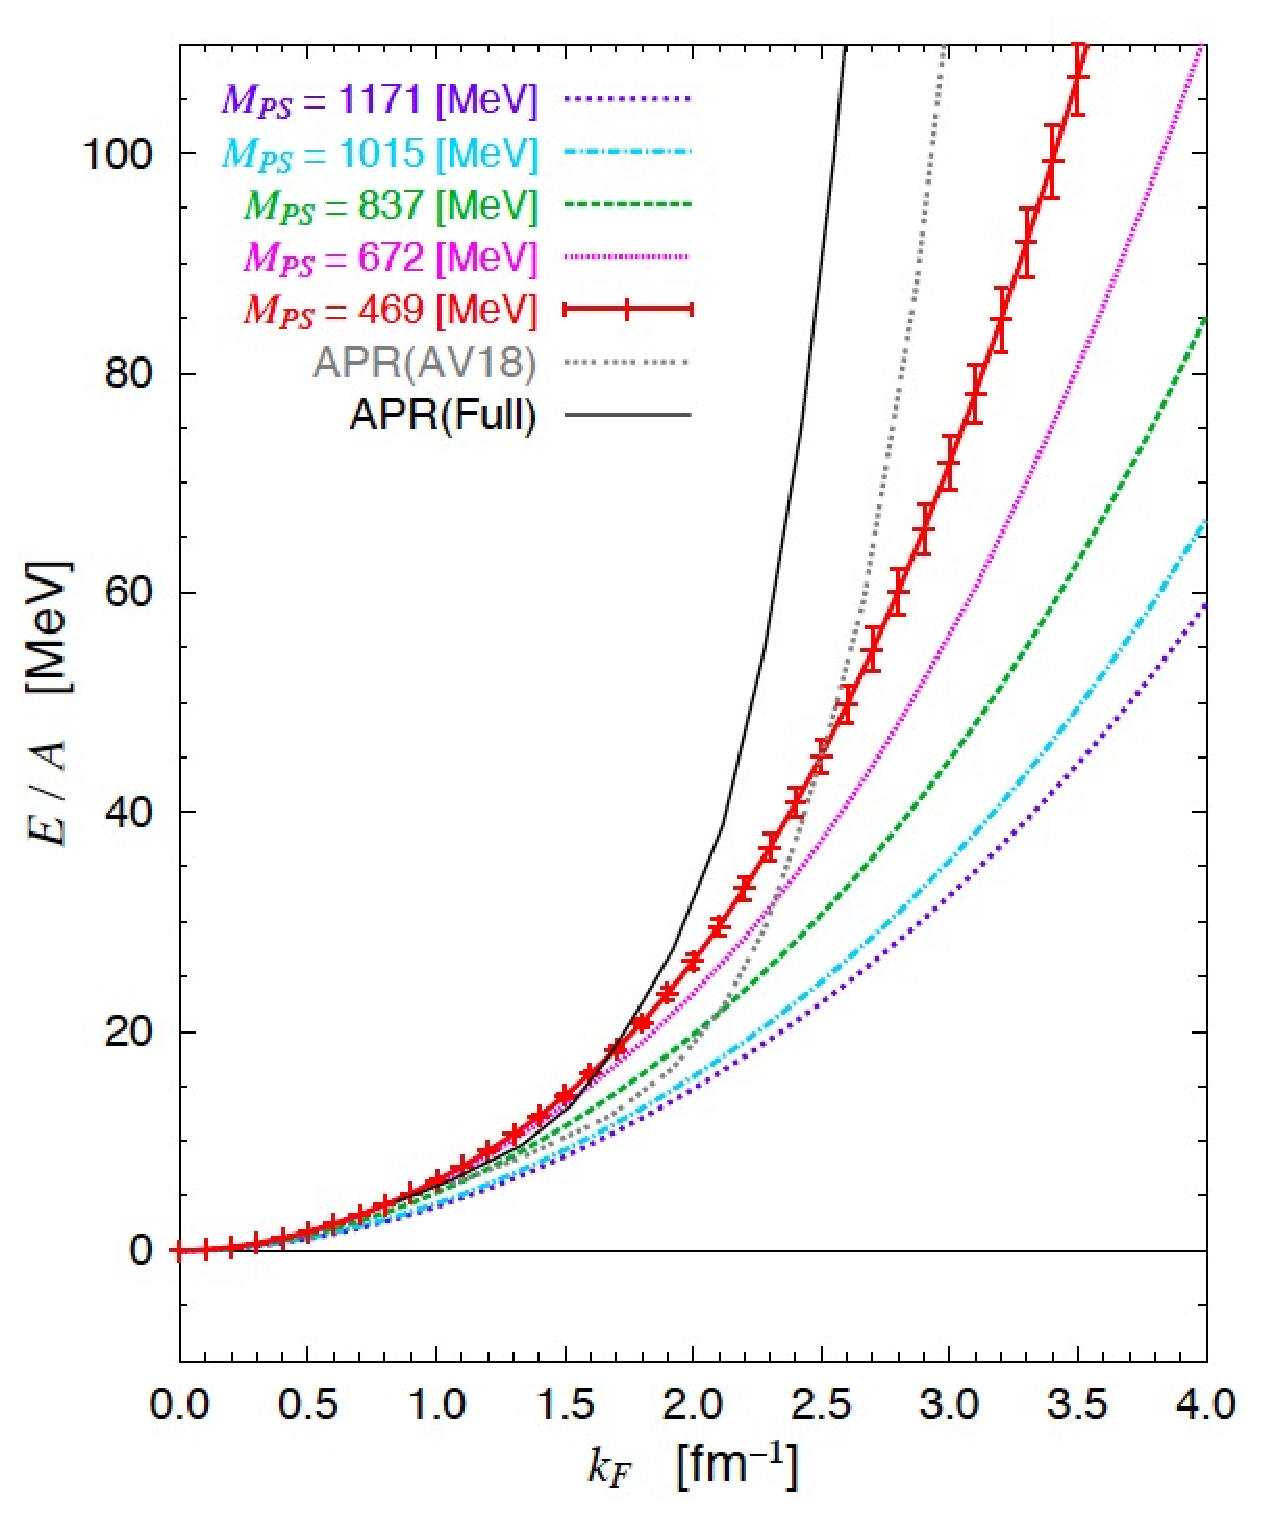
\includegraphics[scale=0.27]{Chapter3-figures/neutron-matter.eps}
 \end{center}
\caption{(Left) Phase shifts of the NN scattering as a
function of energy in the laboratory frame, extracted from
LQCD data at the pion mass 469 MeV in the flavor-SU(3) limit.
 The black and gray dashed lines are the results of the partial wave
analysis (PWA) of the experimental data. (Right) Ground state energy per neutron for the
pure neutron matter as a function of the Fermi momentum.
 The APR with black dotted line (black solid line)   corresponds to the empirical equation of state without (with) the
phenomenological three nucleon force \cite{Akmal:1998cf}.
 \cite{Akmal:1998cf}.
The figures are taken from \cite{Inoue:2013nfe}.
  }
\label{fig:NN-phase_shift}
\end{figure}
%%%%%%%%%%%%%%%%%%%%%%%%%%%%%%


Shown in Fig.\ref{fig:NN-potential}  are the results of the exploratory study of the potentials
obtained by LQCD simulations on the lattice  with $a\simeq 0.12$ fm, 
$L\simeq 4$ fm and 3 degenerate flavours  \cite{Inoue:2011ai}.  Corresponding pion mass ranges from
 469 MeV to 1171 MeV. 
\begin{itemize}
\item  The upper left panel is the 
central potential $V^{({\bf 27})}(r)$ to which the  $^1S_0$ nucleon-nucleon potential belongs.
 It  has a repulsive core at short distance and an attractive pocket at intermediate distance.
As the pion mass decreases,  the repulsive core gets stronger and the attractive tail gets
 longer.  
\item As shown in the lower left panel, the structure of the potential is quite different for $V^{({\bf 1})}(r)$ to which the
  flavour singlet $H$ dibaryon (composed of $uuddss$) belongs.   There is no repulsive core and the attraction 
  increases as the pion mass decreases.  Such a feature is consistent with the 
   notion of  the quark Pauli principle previous discussed in phenomenological quark models \cite{Oka-Fujiwara}.
\item The upper and lower right panels of  Fig.\ref{fig:NN-potential}  are the 
central potential and the tensor potential of $V^{({\bf 10}^*)}(r)$, respectively. The
$^3S_1$ nucleon-nucleon potential belongs to this channel. The central part has a similar
structure as the $^1S_0$ channel, while the tensor part has strong attraction and grows rapidly  as the 
 pin mass decreases.  The latter aspect is qualitatively consistent with the one-pion-exchange picture at
 long distances.
 \end{itemize}
   
 Shown in  Fig.\ref{fig:NN-phase_shift} (left) is  the nucleon-nucleon scattering phase shifts
  in the $^1S_0$ channel and $^3S_1$ channel obtained by using the 
   potentials, $V^{({\bf 27})}(r)$ and $V^{({\bf 10}^*)}(r)$,  for the pion mass 469 MeV \cite{Inoue:2013nfe}.
   The qualitative feature of the 
   phase shift in the $^1S_0$ channel is similar to the experimental one denoted by the 
   black solid  line, despite the fact that pion mass in the simulation is  more than 3 times
   heavier than the physical value. In the  $^3S_1$ channel, the deuteron bound state is 
   not formed yet due to heavy pion mass, so that the phase shift starts from 0 at zero energy
    in contrast the the experimental one denoted by the black dashed line.
    There is however a tendency that the attraction in the $^3S_1$ channel is larger than
   the $^1S_0$ channel even for the heavy pion mass.
  Shown in  Fig.\ref{fig:NN-phase_shift} (right) is  the energy per particle $E/A$ as a function of the 
  fermi momentum $k_{\rm F}$ for pure neutron matter calculated by using the Brueckner-Hartree-Fock method
  with the neutron-neutron potential in the $^1S_0$ channel in Fig.\ref{fig:NN-phase_shift} (left). 
 As the pion mass decreases, the equation of state becomes stiffer due to the growth of the repulsive  core. 
 The APR with black dotted line (black solid line)   corresponds to the empirical equation of state without (with) the
phenomenological three nucleon force  \cite{Akmal:1998cf}.

 We note that calculations of the baryon-baryon interactions  with  
  (2+1)-flavour LQCD on a large volume ($L \simeq 8.2 {\rm fm}$, $a\simeq 0.085$ fm) at
   nearly the physical quark mass ($m_{\pi}\simeq146$ MeV, $m_{K}\simeq$ 525 MeV)
   are underway  \cite{Doi:2015oha}.
 
  
%%%%%%%%%%%%%
\section{Exercises}
%%%%%%%%%%%%%

\begin{prob} \label{prob:1}
Prove the properties of the Wilson line, Eqs.(\ref{eq:5.wilson-line-i}), (\ref{eq:5.wilson-line-ii}), and (\ref{eq:5.wilson-line-iii}).
\end{prob}

\begin{prob}\label{prob:2}
Derive the expression on $U_{\mu \nu}(n)-1$ in 
Eq.(\ref{eq:5.wilson-plaq-cont-2}) by using the Baker-Campbell-Hausdorff formula.
\end{prob}

\begin{prob}\label{prob:3}
Show the $\Gamma_5$ Hermiticity of the Dirac operator in Eq.(\ref{eq:gamma5-hermite}).
\end{prob}

\begin{prob}\label{prob:4}
Derive  the free fermion propagator on the lattice in the momentum representation,
Eqs.(\ref{eq:DF}) and (\ref{eq:Mp}). 
\end{prob}

\begin{prob}\label{prob:5}
Analyze the dispersion relation of the free fermion associated with the 
Dirac operator, $D_{\rm GW}$ in Eq.(\ref{eq:5.overlap-op}).
\end{prob}

\begin{prob}\label{prob:6}
Derive the group integration formulas, Eq.(\ref{eq:group-int-1})- Eq.(\ref{eq:group-int-B}), by taking appropriate 
contractions of the color indices.
\end{prob}


\begin{prob}\label{prob:7}
Derive the formula for the Wilson loop in the strong coupling limit Eq.(\ref{eq:5.wilson-strong}) by using the group integration formulas
Eqs.(\ref{eq:group-int-0})-(\ref{eq:group-int-2}). 
\end{prob}

\begin{prob}\label{prob:8}
Derive the lattice coupling $g(a)$ as a function of the lattice spacing $a$, Eq.(\ref{eq:5.lat-running-g}).
\end{prob}

\begin{prob}\label{prob:9}
Show the convergence of $W[\phi]$ to the equilibrium distribution $W_{\rm eq}[\phi]$
under the Markov process by introducing the distance $D= \sum_{\phi} \left| W[\phi] -W_{\rm eq}[\phi] \right| $
 and by studying its behavior under update.
\end{prob}

\begin{prob}\label{prob:10}
Prove that the Metropolis test in Eq.(\ref{eq:MET-test})
satisfies the detailed balance Eq.(\ref{eq:DT-balance}).
\end{prob}

\begin{prob}\label{prob:11}
Derive the equation of motion for $P_l$ in Eq.(\ref{eq:EOM-P})
from Eq.(\ref{eq:EOM-U}) and  Eq.(\ref{eq:EOM-H}).
\end{prob}

\begin{prob}\label{prob:12}
Prove that the jackknife average and variance for $f({\cal O})={\cal O}$ reduce to the 
standard mean and unbiased variance, respectively.
\end{prob}

\begin{prob}\label{prob:13}
Prove that  the leapfrog integrator satisfies the reversibility Eq.(\ref{eq:reversible}) exactly.
Also prove that  the leapfrog integrator preserves the phase space area exactly by
evaluate the Jacobian, $d\phi' d\pi'= J d\phi d\pi $. 
\end{prob}
 

%%%%%%%%%%%%%%%%
\begin{acknowledgement}
%%%%%%%%%%%%%%%%
%If you want to include acknowledgments of assistance and the like at the end of an individual chapter 
%please use the \verb|acknowledgement| environment -- it will automatically render Springer's preferred layout.
The author thanks Takumi Doi and Atsushi Nakamura for useful comments and information on various aspects of
LQCD simulations.
He also thank the members of HAL QCD Collaboration for  fruitful discussions on the hadron-hadron interactions 
on the lattice.
This work was supported in part by MEXT SPIRE and JICFuS and also by RIKEN iTHES Project.
\end{acknowledgement}
%

\section{Appendix}
\addcontentsline{toc}{section}{Appendix}

%%%%%%%%%%%%%%%%%%%%%%%%%%%%
\subsubsection*{\center{Four vectors and Dirac matrices}}
%%%%%%%%%%%%%%%%%%%%%%%%%%%%

In the (3+1)-dimensional  Minkowski spacetime, coordinates, derivatives 
and four vectors with $\mu=0,1,2,3$ are
\beq
x^{\mu} = (t, \mathbf{x}),
\ \ \partial^{\mu}   =  (\partial_t, -\nabla),
\ \  A^{\mu} =(A^0, \mathbf{A}).
\label{eq:B.vector-M}
\eeq
In the 4-dimensional Euclidean space, 
 we define the corresponding vectors  for $\mu=4,1,2,3$ as
 \beq
(x_{\mu})^{\rm E} = (\tau=it, \mathbf{x}),
\ \ (\partial_{\mu})^{\rm E}   =  (\partial_\tau = -i \partial_{t}, \nabla),
\ \  (A_{\mu})^{\rm E}  =(A_4=iA^0,\mathbf{A}).
\label{eq:B.vector-E}
\eeq


In the (3+1)-dimensional  Minkowski spacetime with the 
 metric $g^{\mu \nu}={\rm diag}(1,-1,-1,-1)$,
  the Dirac matrices satisfy the following relations for $\mu=0,1,2,3$,
\beq
\{ \gamma^{\mu}, \gamma^{\nu} \} = 2 g^{\mu \nu},
\ \ \left( \gamma^{\mu} \right)^{\dagger} = \gamma^0 \gamma^{\mu} \gamma^0,
\ \ \gamma^5 &=& i \gamma^0 \gamma^1 \gamma^2 \gamma^3 
 = \gamma_5 = \left( \gamma_5 \right)^{\dagger}.
\label{eq:B.gamma-min}
\eeq
In the standard Dirac representation, we have
\beq
\gamma^0 = 
\left(  \begin{array}{cc}
        1   & 0   \\
        0   & -1  \\
        \end{array}  \right) , \ \ 
\gamma^j = 
\left(  \begin{array}{cc}
        0           & \sigma_j   \\
        -\sigma_j   & 0          \\
        \end{array}  \right) , \ \ 
\gamma^5 =
\left(  \begin{array}{cc}
        0   & 1   \\
        1   & 0   \\
        \end{array}  \right)  ,
\eeq
where $\sigma_j$ are the Pauli matrices;        
$
%\beq
\sigma_1 = 
\left(  \begin{array}{cc}
        0   & 1   \\
        1   & 0   \\
        \end{array}  \right) , 
\sigma_2 = 
\left(  \begin{array}{cc}
        0           & -i   \\
        i           & 0    \\
        \end{array}  \right) , 
\sigma_3 =
\left(  \begin{array}{cc}
        1   & 0    \\
        0   & -1   \\
        \end{array}  \right)  .
%\label{eq:B.Pauli-matrix}
%\eeq
$

In the 4-dimensional Euclidean space  with the metric
 $\delta_{\mu \nu}={\rm diag}(1,1,1,1)$, we define
  the Euclidean Dirac matrices as
 \beq
  \Gamma_{\mu}  \equiv
 \left(\gamma_4= \gamma^0, -i \mathbf{\gamma} \right),  
 \ \ \Gamma_{-\mu} \equiv  - \Gamma_{\mu}, 
  \ \ {\rm and}   \ \ \Gamma_5 \equiv \gamma^5,
  \eeq
 which satisfy the relations,
 \beq
 \{ \Gamma_{\mu}, \Gamma_{\nu} \}  = 2 \delta_{\mu \nu},
\ \ \Gamma_{\mu}^{\dagger} = \Gamma_{\mu} , 
\ \ \ \ ({\rm for} \ \mu=1,2,3,4,5) 
\label{eq:B.gamma-lat} 
\eeq 

%%%%%%%%%%%%%%%%%%%%%
\subsubsection*{\center{SU$(N)$ algebra}}
%%%%%%%%%%%%%%%%%%%%%

Let ${\cal T}^a$ ($a=1, \cdots , N^2-1$) are the 
 Hermitian generators of the SU$(N)$ group. They satisfy
  the Lie algebra  \index{Lie algebra}
\beq
\left[  {\cal T}^a , {\cal T}^b \right] = i f_{abc} {\cal T}^c ,
\eeq
where $f_{abc}$ is the structure constant \index{structure constants}
 being totally anti-symmetric in its indices.
 $({\cal T}^b)^2$ commutes with every generator ${\cal T}^a$
  and   is called the quadratic Casimir operator. 
  
 For $N=2$, $f_{abc}$ reduces to the  anti-symmetric
 tensor $\epsilon_{ijk}$ with  $\epsilon_{123}=1$.
For $N=3$, the non-vanishing components of $f_{abc}$ read
$f_{123}=1, f_{147}=-f_{156}=f_{246}=f_{257}=f_{345}=-f_{367}=1/2,  
f_{458}=f_{678}= {\sqrt{3}}/{2}$.
   
  In the fundamental representation, 
 ${\cal T}^a$ is written by the $N \times N$ matrices $t^a$ as
\beq
t^a = \frac{1}{2} \lambda_a,
\eeq
 where $\lambda_a$ for $N=2$ reduce to  the Pauli matrices 
 $\sigma_i$, while  those for $N=3$ reduce to the Gell-Mann matrices.
 
 Some useful relations of $t^a$ for general $N$ are
\beq
\label{eq:tt}
{\rm tr} (t^a t^b) = \frac{1}{2} \delta_{ab}, 
\ \ \ t_{ij}^a t_{kl}^b  =  \frac{1}{2} (\delta_{il}\delta_{jk} -\frac{1}{N} \delta_{ij}\delta_{kl} ),
\ \ \ (t^a t^a)_{ij} = C_{{\rm F}} \delta_{ij},
\ \ \ {\rm with} \ C_{{\rm F}}=\frac{N^2-1}{2N}.
\eeq
   
In the adjoint representation, \index{adjoint representation}
 ${\cal T}^a$ is written by  $(N^2-1) \times (N^2-1)$ matrices $T^a$ as
\beq
(T^a)_{bc} = -i f_{abc} ,
\eeq
which satisfy the relations
\beq
  {\rm tr} (T^a T^b) &=& N \delta_{ab}, 
  \ \ \  (T^a T^a)_{bc} = C_{{\rm A}} \delta_{bc},
  \ \ \  {\rm with} \ C_{{\rm A}}= N.
\eeq



%%%%%%%%%%%%%%%%%%%%%%%%%%%%%%
\subsubsection*{\center{Gaussian and Grassmann integrals}}
%%%%%%%%%%%%%%%%%%%%%%%%%%%%%%
 
Basic Gaussian and Grassmann integrals are 
\beq
 \label{eq:C.gauss-x}
& &\int_{-\infty}^{+\infty} \frac{dx}{\sqrt{2\pi}}\ {\rm e}^{-ax^2/2} 
    =\frac{1}{\sqrt{a}}, \\
 \label{eq:C.gauss-z}
& & \int \frac{dz^* dz}{2 \pi i}\ {\rm e}^{-b |z|^2} = \frac{1}{b}, \\
 \label{eq:C.gauss-xi}
& & \int d\bar{\xi} d\xi\  {\rm e}^{- c \bar{\xi} \xi} = c .
\eeq     
Here $x$ ($z$) is a real (complex) number, while $\bar{\xi}$ and
 $\xi$ are anti-commuting Grassmann numbers ($\{ \xi, \bar{\xi} \} =0$,
 and  $\xi^2 = \bar{\xi}^2=0$).
 $a$ and $b$ are assumed to be real and positive numbers, while $c$ is an
  arbitrary complex number.
 Eq.(\ref{eq:C.gauss-z}) can be shown by rewriting the integral 
 in terms of the real and imaginary parts of $z$ or in terms of the 
 polar coordinates of $z$.   Eq.(\ref{eq:C.gauss-xi})
  can be shown by noting that 
   ${\rm e}^{-c\bar{\xi}\xi} = 1- c \bar{\xi}{\xi}$
   and $ \int d\xi = \partial/\partial \xi $
   (integral = derivative) for Grassmann variables.
  
Generalization of the above results to the case of multiple variables
 is straightforward.  For $x =(x_1, \cdots, x_n)$, 
  $z =(z_1, \cdots, z_n)$, $\xi =(\xi_1, \cdots, \xi_n)$,
 and $\bar{\xi} =(\bar{\xi}_1, \cdots, \bar{\xi}_n)$ with
  $\{ \xi_k, \xi_l \} = \{ \bar{\xi}_k, \bar{\xi}_l \} 
   = \{ \xi_k, \bar{\xi}_l \} =0$,  we have
 \beq
 \label{eq:C.gauss-xn}
& &\int \prod_{l=1}^n \frac{dx_l}{ \sqrt{2\pi} }\ 
 {\rm e}^{-\frac{1}{2} x A x} = \frac{1}{\sqrt{{\rm Det}\ A}}, \\
 \label{eq:C.gauss-zn}
& & \int \prod_{l=1}^n \frac{dz_l^* dz_l}{2 \pi i}\ 
{\rm e}^{- z^* B z} = \frac{1}{{\rm Det}\ B}, \\
 \label{eq:C.Z-grass-xin}
& & \int \prod_{l=1}^n d\bar{\xi}_l d\xi_l \
  {\rm e}^{- \bar{\xi}C \xi} = {\rm Det}\ C .
\eeq  
Here $A$ is a non-singular and real-symmetric matrix whose
 eigenvalues $a_l$ satisfy $a_l > 0$ for all $l$.
 $B$ is a non-singular complex matrix whose complex eigenvalues $b_l$
  obtained by the 
  biunitary transformation ($U B V^{\dagger}$)  
  satisfy ${\rm Re}\ b_l > 0$ for all $l$.
 $C$ is an arbitrary complex matrix with no conditions. 
 Note that $B$ and $C$ do not have to be Hermitian matrices.
 In field theories, the label ``$l$" summarizes all possible indices including
  spin, flavor, color, spacetime points etc. and 
  ``${\rm Det}$" denotes the determinant for all these indices. 
 


%%%%%%%%%%%%%%%%%%%%%%%%%%
\subsubsection*{\center{Method of characteristics}}
%%%%%%%%%%%%%%%%%%%%%%%%%%

We need to construct  a general  solution of the 
following partial differential equation,
\beq
 \left( \lambda \frac{\partial}{\partial \lambda} + \beta(g) \frac{\partial}{\partial g} \right) f(\lambda,g)=0.
 \label{eq:MCA-1}
 \eeq
 For this purpose, we introduce the running coupling $\bar{g}(\lambda)$ through 
 $\lambda d\bar{g}/d\lambda = -\beta(\bar{g})$ whose formal solution reads
 \beq
 \lambda = \exp \left( - \int_g^{\bar{g}(\lambda) }  \frac{dg'}{\beta(g')}  \right) .
 \label{eq:MCA-2}
  \eeq
 Then the solution of Eq.(\ref{eq:MCA-1}) can be written as 
 \beq
 f(\lambda, g) = f (1, \bar{g} (\lambda)).
 \eeq
 This can be explicitly checked  by applying the partial derivative on both sides,
 \beq
  \lambda \partial_{\lambda}  f(\lambda,g)&=&
  \lambda (\partial_{\lambda} \bar{g})   (\partial_{\bar{g}} f) = - \beta (\bar{g})  (\partial_{\bar{g}} f) , \nonumber \\
  \beta \partial_g f(\lambda,g) &=&
  \beta(g) \left. (\partial \bar{g}/\partial g) \right|_{\lambda}  (\partial_{\bar{g}} f) = \beta (\bar{g})  (\partial_{\bar{g}} f) .
 \eeq 
 where we have used the  relation $\partial \bar{g}/\partial g = \beta(\bar{g})/\beta(g)$ 
  obtained from   Eq.(\ref{eq:MCA-2}).
 
 In general, the first-order partial differential equation (PDE)  can be transformed to 
 a set of ordinary   differential equations (ODEs) and can  be solved by  {\it the method of characteristics}. 
 As an illustration,  let us consider the following PDE, 
 \beq
  a(t,x) \partial_t u(t,x) + b(t,x) \partial_x f(t,x) = c(t,x).
\label{eq:MCA-3}
 \eeq
This is equivalent to the coupled ODEs,
\beq
\frac{d \bar{t}}{ds}  = a (\bar{t}, \bar{x}) , \ \ 
\frac{d \bar{x}}{ds}  = b (\bar{t}, \bar{x}) , \ \ 
\frac{d f(\bar{t},\bar{x} ) } {ds}  = a (\bar{t}, \bar{x}) ,
\label{eq:MCA-4}
\eeq
where $s$ parametrizes the  "flow" of the coordinates. $(\bar{t}(s), \bar{x}(s))$.
This is called the {\it characteristic curve} as shown in Fig.\ref{fig:char-c}.

\begin{figure}[t]
\begin{center}
%\framebox[74mm]{\rule[-26mm]{0mm}{52mm}}
%\includegraphics[scale=0.6]{as-scale.eps}
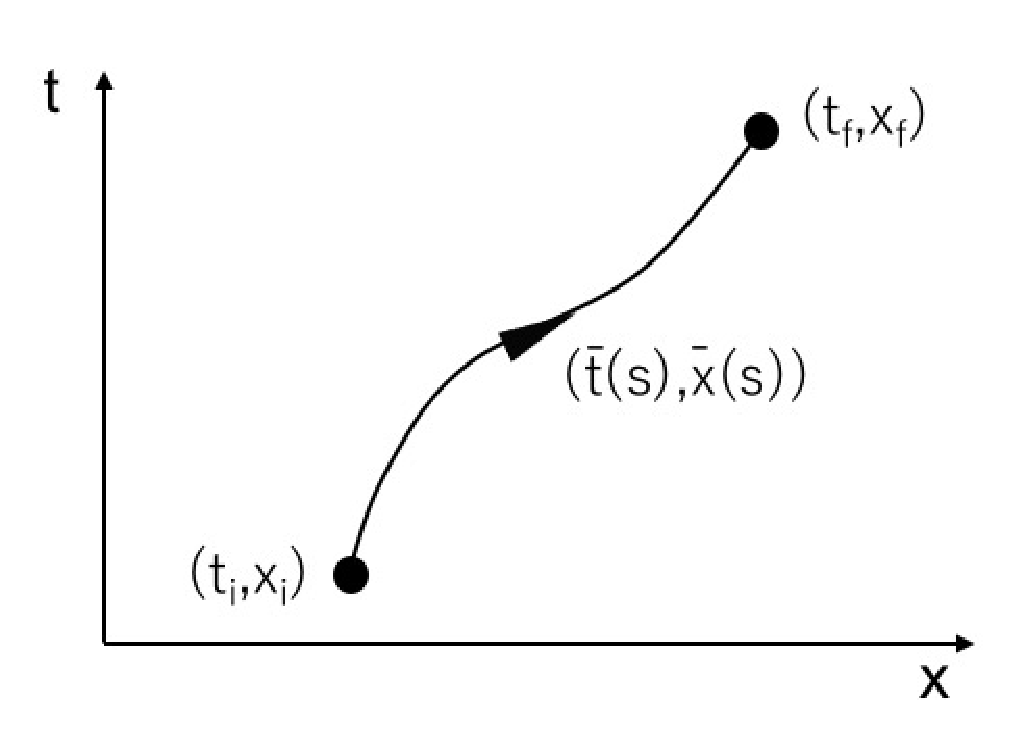
\includegraphics[scale=0.35]{Chapter3-figures/char-c.eps} 
 \end{center}
\caption{Schematic illustration of the characteristic curve.}
\label{fig:char-c}
\end{figure}

The function $f$ can be obtained by integrating the last equation of Eq.(\ref{eq:MCA-4}) 
on the  characteristic curve from the initial point $(t_{\rm i},x_{\rm i})$ to the final point $(t_{\rm f},x_{\rm f})\equiv (t,x)$,
\beq
f(t,x)= f (t_{\rm i}, x_{\rm i}) + h (t, x, t_{\rm i}, x_{\rm i})
\label{eq:MCA-6}
\eeq
where  $h$ stands for an integration of the known function $c(\bar{t},\bar{x})$ on the
characteristic curve.  Eq.(\ref{eq:MCA-6}) implies  that the desired function at $(t,x)$ is obtained 
essential by a "pullback" of the point to $(t_{\rm i},x_{\rm i})$ along the characteristic curve. 
It is a straightforward exercise  to generalize the above derivation to the system with more coordinates,
$(t, \mathbf{x})$.  

%%%%%%%%%%%%%%%%%%%%%%%%%%%%%%%%%%
 \subsubsection*{\center{Leapfrog integrator in molecular dynamics}}
%%%%%%%%%%%%%%%%%%%%%%%%%%%%%%%%%%

Let us start with a Tayler expansion of the field $\phi$:
\beq
\label{eq:LF-phi}
\phi(s+\varepsilon) &=& \phi(s) + \varepsilon \dot{\phi}(s) + \frac{\varepsilon^2}{2} \ddot{\phi}(s) + O(\varepsilon^3), \nonumber \\
&=&  \phi(s) + \varepsilon {\pi}(s) + \frac{\varepsilon^2}{2} \dot{\pi}(s) + O(\varepsilon^3), \nonumber  \\
&=& \phi(s) + \varepsilon {\pi}(s+\varepsilon/2) + O(\varepsilon^3), 
\eeq
where we have used the equation of motion, $\dot{\phi}(s) \equiv d\phi(s)/ds = \pi(s)$.
To evaluate ${\pi}(s+\varepsilon/2)$, we take the midpoint prescription which does not have $O(\varepsilon^2)$ error,
 \beq
 \label{eq:LF-pi}
{\pi}(s+\varepsilon/2)&=&{\pi}(s-\varepsilon/2) + \varepsilon \dot{\pi}(s) + O(\varepsilon^3) \nonumber \\
&=&  {\pi}(s-\varepsilon/2)   - \varepsilon \frac{\delta S(\phi)}{\delta \phi(s)} + O(\varepsilon^3) .
\eeq
Eqs.(\ref{eq:LF-phi}) and (\ref{eq:LF-pi})  give a procedure to move the molecular dynamics one-step forward,
$(\phi(s), \pi(s-\varepsilon/2))  \rightarrow (\phi(s+\varepsilon), \pi(s+\varepsilon/2))$. 
The initial and final steps need to receive special care,
\beq
\pi(\varepsilon/2) = \pi(0) - \frac{1}{2} \varepsilon \frac{\delta S(\phi)}{\delta \phi(s)} + O(\varepsilon^2), \ \ \ 
\pi(s_{\rm f}) =\pi(s_{\rm f}-\varepsilon/2) -  \frac{1}{2} \varepsilon \frac{\delta S(\phi)}{\delta \phi(s_{\rm f})} + 
O(\varepsilon^2),
 \eeq
 which have only $O(\epsilon^2)$ accuracy.  An illustration of this leapfrog integrator is shown in Fig.(\ref{fig:LF}).
 Since the initial and final steps introduce  $O(\varepsilon^2)$ error irrespective of the 
length of the MD trajectory, and  the intermediate steps introduce 
$O(\varepsilon^3) \times \varepsilon^{-1} =O(\varepsilon^2)$ error as a whole,  one finds
 $\Delta H = O(\varepsilon^2)$ after one MD trajectory before the Metropolis test.

The leapfrog integrator satisfies the reversibility and symplectic property, which can be checked explicitly
by using the above definitions (Exercise \ref{prob:13}).
 
 \begin{figure}[t]
\begin{center}
%\framebox[74mm]{\rule[-26mm]{0mm}{52mm}}
%\includegraphics[scale=0.6]{as-scale.eps}
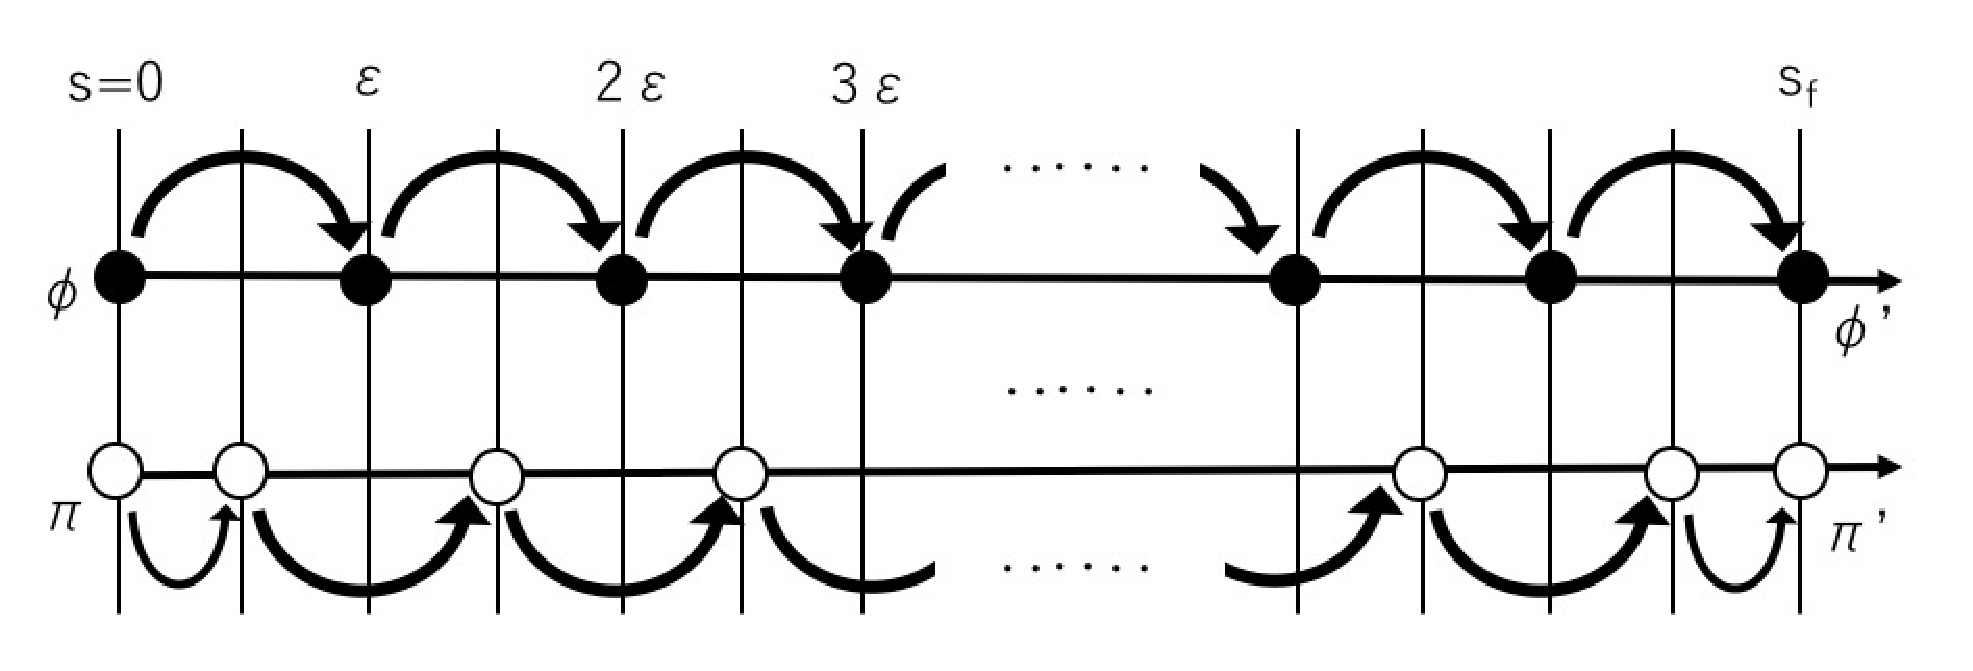
\includegraphics[scale=0.3]{Chapter3-figures/leapfrog.eps} 
 \end{center}
\caption{The leapfrog integrator.}
\label{fig:LF}
\end{figure}


%%%% references %%%%%%%%%
\begin{thebibliography}{99.}%

\bibitem{Wilson:1974sk}
  K.~G.~Wilson, Phys.\ Rev.\ D {\bf 10},  2445  (1974)
  
 \bibitem{Creutz:1980zw}
  M.~Creutz, Phys.\ Rev.\ D {\bf 21},  2308 (1980) 
  
  \bibitem{Brambilla:2014jmp}
  N.~Brambilla {\it et al.}, Eur.\ Phys.\ J.\ C {\bf 74},  2981 (2014)
   
  \bibitem{Wilson:2004de}
  K.~G.~Wilson,  Nucl.\ Phys.\ Proc.\ Suppl.\  {\bf 140},  3 (2005)
  
\bibitem{Creutz:1984mg}
  M.~Creutz, {\em Quarks, gluons and lattices} (Cambridge University Press, 1985)
    
\bibitem{Rothe:1992nt}
  H.~J.~Rothe, World Sci.\ Lect.\ Notes Phys.~{\bf 82}, 1 (2012)

 \bibitem{Hoelbling:2014uea}
  C.~Hoelbling, Acta Phys.\ Polon.\ B {\bf 45},   2143 (2014)


 \bibitem{Ukawa:2015eka}
  A.~Ukawa, J.\ Statist.\ Phys.\  {\bf 160},  1081 (2015)
 
\bibitem{Negele:1988vy}
  J.~W.~Negele and H.~Orland,
 {\em Quantum Many Particle Systems} (Addison-Wesley, 1988)   

\bibitem{Haggstrom:2002}
  O. H\"{a}ggstr\"{o}m,
  {\em Finite Markov Chains and Algorithmic Applications} (Cambridge University Press, 2002)

\bibitem{SuwaTodo:2010}
 H. Suwa and S.Todo,
 Phys.\ Rev.\ Lett.\ {\bf 105},  120603 (2010)

 \bibitem{Duane:1987de}
  S.~Duane, A.~D.~Kennedy, B.~J.~Pendleton and D.~Roweth, Phys.\ Lett.\ B {\bf 195},  216 (1987)

  
\bibitem{Metropolis_1953}
 N. Metropolis, A. W. Rosenbluth, M. N. Rosenbluth, A. H. Teller and E. Teller, J. Chem. Phys. {\bf 21},  1087 (1953)
  
\bibitem{Schaefer:2012tq}
  S.~Schaefer, PoS {\bf LATTICE2012},  001 (2012)
  
 \bibitem{Bali:2000gf}
  G.~S.~Bali, Phys.\ Rept.\  {\bf 343},  1 (2001)

\bibitem{Durr:2008zz}
  S.~Durr {\it et al.}, Science {\bf 322},  1224 (2008)
  
\bibitem{Borsanyi:2014jba}
  S.~Borsanyi {\it et al.}, Science {\bf 347},  1452 (2015)
  
\bibitem{RPP}   
The Review of Particle Physics (2015), \url{http://pdg.lbl.gov/ } 
  
\bibitem{Asakawa:2000tr}
  M.~Asakawa, T.~Hatsuda and Y.~Nakahara,
  Prog.\ Part.\ Nucl.\ Phys.\  {\bf 46} (2001) 459

  
\bibitem{Fodor:2012gf}
  Z.~Fodor and C.~Hoelbling, Rev.\ Mod.\ Phys.\  {\bf 84},  449 (2012)
   
\bibitem{this_book}
Consult other chapters of this volume
 
 \bibitem{Machleidt:2007ms}
  R.~Machleidt, arXiv:0704.0807

\bibitem{Aoki:2013ldr}
  S.~Aoki {\it et al.},
  Eur.\ Phys.\ J.\ C {\bf 74},  2890 (2014)

\bibitem{luescher}
 M.~L\"{u}scher, Nucl. \ Phys.\ B {\bf 354},  531 (1991)

\bibitem{Ishii:2006ec}
N.~Ishii, S.~Aoki and T.~Hatsuda,
Phys.\ Rev.\ Lett.\  {\bf 99},  022001 (2007)

\bibitem{HALQCD:2012aa}
  N.~Ishii {\it et al.} [HAL QCD Collaboration],
 Phys.\ Lett.\ B {\bf 712},  437 (2012)

\bibitem{Iritani:2015dhu}
T.~Iritani [HALQCD Collaboration], arXiv:1511.05246

\bibitem{okubo}
S. Okubo S, R.E. Marshak, Ann. of Phys. {\bf 4},  166 (1958)

\bibitem{Oka-Fujiwara}
M. Oka, K. Shimizu, K. Yazaki, Prog.\ Theor.\ Phys.\ Suppl.\  {\bf 137},   1 (2000)

\bibitem{Inoue:2011ai}
  T.~Inoue {\it et al.} [HAL QCD Collaboration],
  Nucl.\ Phys.\ A {\bf 881},  28 (2012)
  
  \bibitem{Inoue:2013nfe}
  T.~Inoue {\it et al.} [HAL QCD Collaboration],
  Phys.\ Rev.\ Lett.\  {\bf 111},  112503 (2013)
  
 \bibitem{Akmal:1998cf}
  A.~Akmal, V.~R.~Pandharipande and D.~G.~Ravenhall,
  Phys.\ Rev.\ C {\bf 58}, 1804 (1998)
  
  \bibitem{Doi:2015oha}
  T.~Doi {\it et al.} [HAL QCD Collaboration], arXiv:1512.01610
 


  
\end{thebibliography}

% Theoretical aspects of few-body systems and effective field                           \

% theories, Hans-Werner Hammer                                                          \

\title{Theoretical aspects of few-body systems and effective field theories}
\author{Hans-Werner Hammer}
\institute{Hans-Werner Hammer \at Name of institution and address, \email{name@email.address}}
\maketitle
\abstract{Each chapter should be preceded by an abstract (10--15 lines long) that summarizes the content. The abstract will appear \textit{online} at \url{www.SpringerLink.com} and be available with unrestricted access. This allows unregistered users to read the abstract as a teaser for the complete chapter. As a general rule the abstracts will not appear in the printed version of your book unless it is the style of your particular book or that of the series to which your book belongs.\newline\indent
Please use the 'starred' version of the new Springer \texttt{abstract} command for typesetting the text of the online abstracts (cf. source file of this chapter template \texttt{abstract}) and include them with the source files of your manuscript. Use the plain \texttt{abstract} command if the abstract is also to appear in the printed version of the book.}
%\maketile

\section{General Introduction}
\section{More stuff}


\begin{acknowledgement}
If you want to include acknowledgments of assistance and the like at the end of an individual chapter please use the \verb|acknowledgement| environment -- it will automatically render Springer's preferred layout.
\end{acknowledgement}

% Lattice Methods and effective field theory, Amy Nicholson                             \

\label{chap:chapter5}
\newcommand\mpi {m_{\pi}}
%\newcommand\qslash {\slashed{q}}
%\newcommand{\note}[1]{{\bf \textcolor{red}{\uppercase{#1}}}}
\newcommand\pslash {\slashed{p}}
\newcommand\dslash {\slashed{\partial}}
%\newcommand\Dslash {\slashed{D}}
\newcommand\psidag{\psi^{\dagger}}
\newcommand\tautoinfty{\underset{\tau \to\infty}{\longrightarrow}}
\newcommand\Eq[1]{Eq.~(\ref{eq:#1})}
\newcommand\Eqs[2]{Eqs.~(\ref{eq:#1},\ref{eq:#2})}
%\newcommand\Eqs[2]{Eqs.~(\ref{eq:#1})-(\ref{eq:#2})}
\newcommand\Fig[1]{Fig.~\ref{fig:#1}}
\newcommand\Figtwo[2]{Figs.~\ref{fig:#1} and \ref{fig:#2}}
\newcommand\Figs[2]{Figs.~\ref{fig:#1}-\ref{fig:#2}}
\newcommand\Sec[1]{Sec.~\ref{sec:#1}}
\newcommand\Sect[1]{Section~\ref{sec:#1}}
\newcommand\Tab[1]{Table~\ref{tab:#1}}
%\newcommand{\be}{\begin{equation}}
%\newcommand{\ee}{\end{equation}}
%\newcommand\beq{\begin{eqnarray}}
%\newcommand\eeq{\end{eqnarray}} 
\newcommand\eqn[1]{\label{eq:#1}} 
\newcommand\eq[1]{eq.~(\ref{eq:#1})} 
\newcommand\eqstwo[2]{eqs. (\ref{eq:#1},\ref{eq:#2})} 
\newcommand\eqs[2]{eqs. (\ref{eq:#1}-\ref{eq:#2})} 
\newcommand{\vev}[1]{\langle #1 \rangle}
\newcommand{\lfb}{\bigskip\noindent}
\newcommand{\bfn}{{\mathbf n}}
\newcommand{\bfx}{{\mathbf x}}
\newcommand{\bfr}{{\mathbf r}}
\newcommand{\bfk}{{\mathbf k}}
\newcommand{\bfq}{{\mathbf q}}
\newcommand{\bfp}{{\mathbf p}}
\newcommand{\bfP}{{\mathbf P}}
\newcommand\Ncfg{N_{\mbox{\tiny cfg}}}
\newcommand{\eV}{{\rm ~eV }}
\newcommand{\keV}{{\rm ~keV }}
\newcommand{\GeV}{{\rm ~GeV }}
\newcommand{\TeV}{{\rm ~TeV }}
\newcommand{\MeV}{{\rm ~MeV }}
\newcommand{\calA}{{\mathcal{ A}}}
\newcommand{\calB}{{\mathcal{ B}}}
\newcommand{\calC}{{\mathcal{ C}}}
\newcommand{\calD}{{\mathcal{ D}}}
\newcommand{\calE}{{\mathcal{ E}}}
\newcommand{\calF}{{\mathcal{ F}}}
\newcommand{\calI}{{\mathcal{ I}}}
\newcommand{\calH}{{\mathcal{ H}}}
\newcommand{\calO}{{\mathcal{ O}}}
\newcommand{\calM}{{\mathcal{ M}}}
\newcommand{\calN}{{\mathcal{ N}}}
\newcommand{\calP}{{\mathcal{ P}}}
\newcommand{\calR}{{\mathcal{ R}}}
\newcommand{\calG}{{\mathcal{ G}}}
\newcommand{\calQ}{{\mathcal{ Q}}}
\newcommand{\calS}{{\mathcal{ S}}}
\newcommand{\calT}{{\mathcal{ T}}}
\newcommand{\calU}{{\mathcal{ U}}}
\newcommand{\calV}{{\mathcal{ V}}}
\newcommand{\calW}{{\mathcal{ W}}}
\newcommand{\calZ}{{\mathcal{ Z}}}
\newcommand{\calL}{{\mathcal{ L}}}
\newcommand\rf[1]{{\bf [REF #1]}}
\newcommand{\Tr}{{\rm Tr\,}}
\newcommand\half{{\textstyle{\frac{1}{2}}}} 
\newcommand\fourth{{\textstyle{\frac{1}{4}}}} 
\newcommand\expect[3]{\langle #1|#2|#3\rangle}

%
% Young Tableaux:
%
\newcommand{\mybar}[1]%
        {\kern 0.6pt\overline{\kern -0.6pt#1\kern -0.6pt}\kern 0.6pt}
\newcommand{\drawsquare}[2]{\hbox{%
\rule{#2pt}{#1pt}\hskip-#2pt%  left vertical
\rule{#1pt}{#2pt}\hskip-#1pt%  lower horizontal
\rule[#1pt]{#1pt}{#2pt}}\rule[#1pt]{#2pt}{#2pt}\hskip-#2pt%  upper horizontal
\rule{#2pt}{#1pt}}% right vertical
\newcommand{\Yfund}{\raisebox{-.5pt}{\drawsquare{6.5}{0.4}}}%  fund
\newcommand{\Ybarfund}{\mybar{\raisebox{-.5pt}{\drawsquare{6.5}{0.4}}}}%

%\begin{document}
\title{Lattice methods and effective field theory}
\author{Amy Nicholson}
\institute{Amy Nicholson \at Department of Physics, University of California, Berkeley, Berkeley CA 94720, USA, \email{anicholson@berkeley.edu}}
\maketitle
\abstract{Lattice field theory is a non-perturbative tool for studying properties of strongly interacting field theories, which is particularly amenable to numerical calculations and has quantifiable systematic errors. In these lectures we apply these techniques to nuclear Effective Field Theory (EFT), a non-relativistic theory for nuclei involving the nucleons as the basic degrees of freedom. The lattice formulation of \cite{EKLN1,EKLN4} for so-called pionless EFT is discussed in detail, with portions of code included to aid the reader in code development. Systematic and statistical uncertainties of these methods are discussed at length, and extensions beyond pionless EFT are introduced in the final Section.}
\unitlength = 1mm


\section{\label{sec:intro}Introduction}
Quantitative understanding of nuclear physics at low energies from first principles remains one of the most challenging programs in contemporary theoretical physics research. While physicists have for decades used models combined with powerful numerical techniques to successfully reproduce known nuclear structure data and make new predictions, currently the only tools available for tackling this problem that have direct connections to the underlying theory, Quantum Chromodynamics (QCD), as well as quantifiable systematic errors, are Lattice QCD and Effective Field Theory (EFT). Combined, these techniques may be used to not only quantify any bias introduced when altering QCD in order to make it computationally tractable, but also to better understand the connection between QCD and nuclear physics.

The lattice is a tool for discretizing a field theory in order to reduce the path integral, with an infinite number of degrees of freedom, to a finite-dimensional ordinary integral. By rendering the dimension finite (though extremely large), the integral may then be estimated on a computer using Monte Carlo methods. Errors introduced through discretization and truncation of the region of spacetime sampled are controlled through the spatial and temporal lattice spacings, $b_s,b_{\tau}$, and the spatial and temporal lengths, $L,\beta$. Thus, these errors may be quantified through the lattice spacing dependence of the observables, and often may be removed through extrapolation to the continuum and infinite volume limits.

LQCD is a powerful and advanced tool for directly calculating low-energy properties of QCD. However, severe computational issues exist when calculating properties of systems with nucleons. Unfortunately, these problems grow rapidly with the number of nucleons in the system. 

The first issue is the large number of degrees of freedom involved when using quark fields to create nucleons. In order to calculate a correlation function for a single nucleon in LQCD using quarks (each of which has twelve internal degrees of freedom given by spin and color), one has to perform all possible Wick contractions of the fields in order to build in fermion antisymmetrization. For example, to create a proton using three valence quark operators requires the calculation of two different terms corresponding to interchanging the two up quark sources. The number of contractions involved for a nuclear correlation function grows with atomic number $Z$ and mass number $A$ as $(A+Z)!(2A-Z)!$. For He$_4$ this corresponds to $\sim 5 \times 10^5$ terms\footnote{This is a very na\"ive estimate; far more sophisticated algorithms exist with power-law scaling.}!

The second major problem occurs when performing a stochastic estimate of the path integral. A single quark propagator calculated on a given gauge field configuration may be a part of either a light meson or a heavy nucleon. However, the difference cannot be determined until correlations with the other quark fields present are built in by summing over a sufficiently large number of these field configurations\footnote{This interpretation of the signal-to-noise problem has been provided by David B. Kaplan.}. This leads to large fluctuations from configuration to configuration, and a stochastic signal-to-noise ratio, $\calR$, which degrades exponentially with the number of nucleons in the system,
\beq
\calR \sim e^{-A(M-3/2 m_{\pi})\tau} \ ,
\eeq
where $M$ is the nucleon mass and $m_{\pi}$ is the pion mass \cite{Lepage:1989hd}. This is currently the major limiting factor for the size of nuclear which can be probed using LQCD. The best calculations we have from LQCD using multiple nucleons to date are in the two-nucleon sector \cite{Berkowitz:2015eaa,Kurth:2015cvl,Nicholson:2015pys,Orginos:2015aya,Detmold:2015daa,Chang:2015qxa,Beane:2015yha,Beane:2014sda,Beane:2014ora,Beane:2013br,Beane:2012vq,Beane:2011iw,Beane:2009py,Yamazaki:2015vjn,Yamazaki:2015asa,Yamazaki:2013rna,Yamazaki:2012fn,Yamazaki:2012hi,Doi:2015uvd,Doi:2015oha,Ishii:2006ec,Murano:2013xxa,Aoki:2014mia,Murano:2013gta,HALQCD:2012aa,Inoue:2010hs}, while fewer calculations have been performed for three and four nucleon systems \cite{Beane:2009gs,Beane:2012vq,Beane:2014ora,Beane:2014sda,Chang:2015qxa,Yamazaki:2015vjn,Yamazaki:2015asa,Yamazaki:2013rna,Yamazaki:2012fn,Yamazaki:2012hi,Doi:2011gq}; however, even for two nucleon systems unphysically large pion masses must be used in order to reduce the noise problem. We will discuss signal-to-noise problems in more detail in \Sec{SNR}. 

Starting from an EFT using nucleons as the fundamental degrees of freedom greatly reduces the consequences from both of these issues. EFTs also enjoy the same benefit as the lattice over traditional model techniques of having quantifiable systematic errors, this time controlled by the cutoff of the EFT compared to the energy regime studied. For chiral EFTs this scale is generally $\Lambda_{\chi} \sim m_{\rho} \sim 700$ MeV. Systematic errors can be reduced by going to higher orders in an expansion of $p/\Lambda_{\chi}$, where $p$ is the momentum scale probed, with the remaining error given by the size of the first order which is not included. In a potential model there is no controlled expansion, and it is generally unknown how much the results will be affected by leaving out any given operator. In addition, field theories provide a rigorous mathematical framework for calculating physical processes, and can be directly translated into a lattice scheme.

Our discussion will begin with understanding a very basic nuclear EFT, pionless EFT, at leading order. We will then proceed to discretize this theory and set up a framework for performing Monte Carlo calculations of our lattice theory. We will then discuss how to calculate observables using the lattice theory, and how to understand their associated statistical uncertainties. Next we will discuss quantifying and reducing systematic errors. Then we will begin to add terms to our theory going beyond leading order pionless EFT. Finally, we will discuss remaining issues and highlight some successes of the application of these methods by several different groups.

\section{Basics of Effective Field Theory and Lattice Effective Field Theory}
\subsection{\label{sec:EFT}Pionless Effective Field Theory}
The EFT philosophy that we will follow is to write down all possible operators involving the relevant degrees of freedom within some energy range (determined by the cutoff) that are consistent with the symmetries of the underlying theory. Each operator will be multiplied by an unknown low-energy constant which may be fixed by comparing an observable with experiment or lattice QCD. In order to reduce this generally infinite number of operators to a finite number we must also establish a power-counting rule for neglecting operators that do not contribute within some desired accuracy. This is a notoriously difficult problem for nuclear physics, and is in general observable and renormalization scheme dependent. Here, we will only briefly touch upon two common power-counting schemes, the so-called Weinberg and KSW expansions \cite{Weinberg:1990rz,Weinberg:1991um,Kaplan:1996xu,Kaplan:1998tg,Kaplan:1998we}. For reviews of these and other power-counting schemes, see \cite{Epelbaum:2008ga,Epelbaum:2010nr,Machleidt:2011zz}.

The simplest possible nuclear EFT involves non-relativistic nucleon fields interacting via delta functions. This is known as a pionless EFT, and is only relevant for energy scales up to a cutoff $\Lambda \sim m_{\pi}$. Below this scale, the finite range of pion exchange cannot be resolved, and all interactions appear to be point-like. In this discussion we will closely follow that of Ref.~\cite{Kaplan:2005es}. For the moment, let's just consider a theory of two-component (spin up/down) fermion fields, $\psi$, with the following Lagrangian,
\beq
\label{eq:leff}
\mathcal{L}_{\mbox{\tiny eff}} = \psi^{\dagger}\left( i \partial_{\tau} + \frac{\nabla^2}{2M}\right) \psi + g_0 \left(\psi^{\dagger}\psi\right)^2 + \frac{g_2}{8}\left[ \left(\psi\psi\right)^{\dagger}\left(\psi\overleftrightarrow{\nabla}^2\psi\right)+ \mbox{\tiny h.c.}\right]+\cdots \ ,
\eeq
where
\beq
\overleftrightarrow{\nabla}^2 \equiv \overleftarrow{\nabla}^2-2\overleftarrow{\nabla} \cdot \overrightarrow{\nabla}+\overrightarrow{\nabla}^2 \ ,
\eeq
$M$ represents the nucleon mass, $g_0, g_2, \ldots$ are unknown, low-energy constants (LECs) which may be fixed by comparing to experimental or LQCD results, and all spin indices are suppressed. Because the effective theory involves dynamical degrees of freedom that are only relevant up to a certain scale, we must define a cutoff, $\Lambda$, above which the theory breaks down. In general, the LECs scale as $\Lambda^{-\mbox{\tiny dim}(\mathcal{O})}$, where dim$(\mathcal{O})$ represents the dimension of the operator associated with the LEC. According to na\"ive power counting, the $g_2$ term in \Eq{leff} should be suppressed relative to the $g_0$ term, because adding a derivative to an operator increases its dimension. One should be careful in practice, however, because na\"ive power counting does not always hold, as we will see several times throughout these lectures. 

\subsubsection{\label{sec:scatamp}Two particle scattering amplitude}
In order to set the coefficients $g_0, g_2, \ldots$, we may look to experimental scattering data. In particular, if we wish to set the $g_0$ coefficient we should consider two-particle $s$-wave scattering because the operator associated with $g_0$ contains no derivatives. $g_2$ and other LECs may be set using $p$- and higher-wave scattering data. Recall that the S-matrix for non-relativistic scattering takes the following form:
\beq
S=1+\frac{iMp}{2\pi}A \ ,
\eeq
where $p$ is the scattering momentum and $A$ is the scattering amplitude. For $s$-wave scattering the amplitude may be written as,
\beq
\label{eq:Apcotd}
A=\frac{4\pi}{M} \frac{1}{p\cot\delta - ip} \ ,
\eeq
where $\delta$ is the $s$-wave scattering phase shift. Given a short-range two-body potential, the scattering phase shift has a well-known expansion for low momenta, called the effective range expansion,
\beq
\label{eq:ere}
p\cot\delta = -\frac{1}{a}+\frac{1}{2}r_0p^2+r_1p^4+\cdots \ ,
\eeq
where $a$ is the scattering length, $r_0$ is the effective range, and $r_1$ and higher order terms are referred to as shape parameters. The effective range and shape parameters describe the short-range details of the potential, and are generally of order of the appropriate power of the cutoff in a naturally tuned scenario. 

The scattering length may be used to describe the asymptotic behavior of the radial wavefunction. In particular, consider two-particles interacting via an attractive square-well potential. If the square-well is sufficiently strongly attractive, the wavefunction turns over and goes to zero at some finite characteristic length. This means the system is bound and the size of the bound state is given by the scattering length, $a$. On the other hand, if the wavefunction extends over infinite space, then the system is in a scattering state and the scattering length may be determined as the distance from the origin where the asymptote of the wavefunction intersects the horizontal axis (see \Fig{a0}). This implies that the scattering length in the case of a scattering state is negative. If the potential is tuned to give a system which is arbitrarily close to the crossover point from a bound state to a scattering state, corresponding to infinite scattering length, the state is described as being near unitarity, because the unitarity bound on the scattering cross section is saturated at this point. Note that this implies that the scattering length may be any size and is not necessarily associated with the scale set by the cutoff. However, such a scenario requires fine-tuning of the potential. Such fine-tuning is well-known to occur in nuclear physics, with the deuteron and neutron-neutron $s$-wave scattering being notable examples.

\begin{figure}
\caption{\label{fig:a0}Sketches of two-body radial wavefunctions vs. $r$ corresponding to various scattering lengths. From left to right: $a<0$, $a\to\infty$,$a>0$.}
\includegraphics[width=0.3\linewidth]{Chapter5-figures/al0.png}
\includegraphics[width=0.3\linewidth]{Chapter5-figures/ae0.png}
\includegraphics[width=0.3\linewidth]{Chapter5-figures/ag0.png}
\end{figure}

A many-body system composed of two-component fermions with an attractive interaction is known to undergo pairing between the species (higher $N$-body interactions are prohibited by the Pauli exclusion principle), such as in neutron matter, found in the cores of neutron stars, which is composed of spin up and spin down neutrons. At low temperature, these bosonic pairs condense into a coherent state. If the interaction is only weakly attractive, the system will form a BCS state composed of widely separated Cooper pairs, where the average pair size is much larger than the average interparticle spacing. On the other hand, if the interaction is strongly attractive then the pairs form bosonic bound states which condense into a Bose-Einstein condensate. The crossover between these two states corresponds to the unitary regime, and has been studied extensively in ultracold atom experiments, where the interaction between atoms may be tuned using a Feschbach resonance. In this regime, the average pair size is equal to the interparticle spacing (given by the inverse density), which defines the only scale for the system. Thus, all dimensionful observables one wishes to calculate for this system are determined by the appropriate power of the density times some dimensionless constant. 

\subsubsection{\label{sec:couplings}Two-body LECs}
Returning to our task of setting the couplings using scattering parameters as input, we might consider comparing \Eq{leff} and \Eq{ere}, to determine the LEC $g_0$ using the scattering length, $g_2$ using the effective range, and so forth. To see how this is done in practice we may compute the scattering amplitude $A$ in the effective theory, and match the coefficients to the effective range expansion. Let's begin using only the first interaction term in the effective theory, corresponding to $g_0$. Diagrammatically, the scattering amplitude may be written as the sum of all possible bubble diagrams (see \Fig{bubblesum}). Because the scattering length may take on any value, as mentioned previously, we cannot assume that the coupling $g_0$ is small, so we should sum all diagrams non-perturbatively. The first diagram in the sum is given by the tree level result, $g_0$. If we assume that the system carries energy $E=p^2/M$, then the second diagram may be labeled as in \Fig{loop}, and gives rise to the loop integral,
\beq
\label{eq:loop}
I_0 = i\int \frac{d^4q}{(2\pi)^4}\frac{1}{\left(E/2+q_0-\frac{q^2}{2M}-i\epsilon\right)\left(E/2-q_0-\frac{q^2}{2M}+i\epsilon\right)} \ .
\eeq 
Performing the integral over $q_0$ and the solid angle gives
\beq
\label{eq:loopEFT}
I_0 &=& \frac{1}{2\pi^2}\int^{\pi\Lambda/2} dq\frac{q^2}{\left(E-\frac{q^2}{M}\right)} \\
&=& \frac{M}{2\pi^2}\left[\frac{\pi\Lambda}{2}-\sqrt{ME}\tanh^{-1}\left(\frac{\Lambda}{\sqrt{ME}}\right)\right] \ ,
\eeq
where I have introduced a hard momentum cutoff, $\Lambda$. Removing the cutoff by taking it to infinity results in
\beq
I_0 \underset{\Lambda\to\infty}{\longrightarrow}\frac{M}{4\pi}\left[\Lambda+ip\right] \ .
\eeq
Because the interaction is separable, the $n$th bubble diagram is given by $n$ products of this loop function. Thus, the scattering amplitude is factorizable, and may be written
\beq
\label{eq:Abubble}
A&=&g_0\left[1+\sum_n\left(g_0I_0\right)^n\right] \\
&=& \frac{g_0}{1-g_0I_0} \ .
\eeq
We may now compare \Eqs{Apcotd}{ere} and \Eq{Abubble} to relate the coupling $g_0$ to the scattering phase shift. This is easiest to do by equating the inverse scattering amplitudes,
\beq
\frac{1}{A} &=& \frac{1}{g_0}-\frac{M}{4\pi}\Lambda -\frac{iMp}{4\pi} = -\frac{M}{4\pi a}-\frac{iMp}{4\pi} \ ,
\eeq
where I have used \Eq{ere} cut off at leading order. We now have the relation
\beq
g_0 = \frac{4\pi}{M} \frac{1}{\Lambda-1/a} 
\eeq
between the coupling and the physical scattering length. 

\begin{figure}
\caption{\label{fig:bubblesum}Two-body scattering amplitude represented as a sum of bubble diagrams corresponding to a single contact interaction with coupling $g_0$.}
\includegraphics[width=\linewidth]{Chapter5-figures/simple1}
\end{figure}

\begin{figure}
\caption{\label{fig:loop}Feynman diagram for a single bubble in \Fig{bubblesum}, giving rise to the loop integral \Eq{loop}.}
\includegraphics[width=\linewidth]{Chapter5-figures/loop1}
\end{figure}

Note that the coupling runs with the scale $\Lambda$; the particular dependence is determined by the regularization and renormalization scheme chosen. In order to understand the running of the coupling we may examine the beta function. To do so we first define a dimensionless coupling,
\beq
\hat{g}_0 \equiv -\frac{M\Lambda}{4\pi}g_0 \ ,
\eeq
then calculate
\beq
\label{eq:beta}
\beta\left(\hat{g}_0\right) \equiv \Lambda \frac{\partial \hat{g}_0}{\partial \Lambda} = -\frac{a\Lambda}{\left(a\Lambda-1\right)^2} = -\hat{g}_0\left(\hat{g}_0-1\right) \ .
\eeq
This function is a simple quadratic that is plotted in \Fig{beta}. The beta function has two zeroes, $\hat{g}_0 = 0,1$, corresponding to fixed points of the theory. At a fixed point, the coupling no longer runs with the scale $\Lambda$, and the theory is said to be scale-invariant (or conformal, given some additional conditions). This means that there is no intrinsic scale associated with the theory. The fixed point at $\hat{g}_0=0$ is a trivial fixed point, and corresponds to a non-interacting, free field theory (zero scattering length). The other, non-trivial fixed point at $\hat{g}_0=1$ corresponds to a strongly interacting theory with infinite scattering length; this is the unitary regime mentioned previously. Here, not only does the scattering length go to infinity, as does the size of the radial wavefunction, but the energy of the bound state (as approached from $\hat{g}_0 > 1$) goes to zero and all relevant scales have vanished. Note that this is an unstable fixed point; the potential must be finely tuned to this point or else the theory flows away from unitarity as $\Lambda \to 0$ (IR limit).

\begin{figure}
\caption{\label{fig:beta}Beta function (\Eq{beta}) for the two-body contact interaction. Arrows represent the direction of flow toward the IR.}
\includegraphics[width=0.5\linewidth]{Chapter5-figures/beta.pdf}
\end{figure}

Generally perturbation theory is an expansion around free field theory, corresponding to a weak coupling expansion. This is the approach used as part of the Weinberg power counting scheme for nuclear EFT \cite{Weinberg:1990rz,Weinberg:1991um}. However, in some scattering channels of interest for nuclear theory the scattering length is indeed anomalously large, such as the $^1S_0$ and $^3S_1$ nucleon-nucleon scattering channels, where
\beq
a_{^1S_0} &\sim& -24 \mbox{ fm} \ , \\
a_{^3S_1} &\sim& 5 \mbox{ fm} \ .
\eeq
Such large scattering lengths suggest that an expansion around the strongly coupled fixed-point of unitarity may be a better starting point and lead to better convergence. This approach was taken by Kaplan, Savage, and Wise and led to the KSW power-counting scheme \cite{Kaplan:1998we,Kaplan:1998tg,Kaplan:1996xu}. Unfortunately, nuclear physics consists of many scales of different sizes and a consistent power-counting framework with good convergence for all observables has yet to be developed; in general the convergence of a given scheme depends on the scattering channels involved. 

Because nuclear physics is not weakly coupled in all channels, non-perturbative methods, such as lattice formulations, will be favorable for studying few- and many-body systems, where two-body pairs may interact through any combination of channels simultaneously. Due to the scale-invariant nature of the unitary regime, it provides a far simpler testbed for numerical calculations of strongly-interacting theories, so we will often use it as our starting point for understanding lattice EFT methods. 

\subsection{\label{sec:LEFT}Lattice Effective Field Theory}

Our starting point for building a lattice EFT will be the path integral formulation of quantum field theory in Euclidean spacetime. The use of Euclidean time allows the exponent of the path integral to be real (in certain cases), a property which will be essential to our later use of stochastic methods for its evaluation. Given a general theory for particles $\psi,\psi^{\dagger}$ obeying a Lagrangian density \beq 
\mathcal{L}(\psi^{\dagger},\psi) = \psi^{\dagger}\left( \partial_{\tau}-\mu \right)\psi+ \mathcal{H}\left[\psi^{\dagger}, \psi\right] \ ,
\eeq
where $\tau$ is the Euclidean time, $\mu$ the chemical potential, and $\mathcal{H}$ is the Hamiltonian density, the Euclidean path integral is given by
\beq
Z=\int \mathcal{D} \psi^{\dagger}\mathcal{D} \psi e^{-\int d\tau d^3x\left[\mathcal{L}(\psi^{\dagger},\psi)\right]} \ .
\eeq
If the integral over Euclidean time is compact, then the finite time extent $\beta$ acts as an inverse temperature, and we may draw an analogy with the partition function in statistical mechanics, $Z = tr\left[e^{-H\beta}\right]$. This analogy is often useful when discussing lattice formulations of the path integral. In this work we will generally consider $\mu=0$ and create non-zero particle density by introducing sources and sinks for particles and calculating correlation functions. 

We discretize this theory on a square lattice consisting of $L^3 \times N_{\tau}$ points, where $L$ is the number of points in all spatial directions, and $N_{\tau}$ is the number of temporal points. We will focus on zero temperature physics, corresponding to large $N_{\tau}$\footnote{The explicit condition on $N_{\tau}$ required for extracting zero temperature observables will be discussed in \Sec{observables}}. We must also define the physical distance between points, the lattice spacings $b_s, b_{\tau}$, where $b_{\tau} = b_s^2/M$ by dimensional analysis for non-relativistic theories. The fields are now labeled by discrete points, $\psi(\vec{x},\tau) \to \psi_{\vec{n},\tau}$, and continuous integrals are replaced by discrete sums, $\int d^3x \to \sum_{\vec{n},\tau}^{L,N_{\tau}}$.

\subsubsection{Free field theory}
To discretize a free field theory, we must discuss discretization of derivatives. The simplest operator which behaves as a single derivative in the continuum limit is a finite difference operator,
\beq
\partial_{\hat{k}}^{(L)} f_j = \frac{1}{b_s}\left[f_{j+\hat{k}}-f_j\right] \ ,
\eeq
where $\hat{k}$ is a unit vector in the $k$-direction. The discretized second derivative operator must involve two hops, and should be a symmetric operator to behave like the Laplacian. A simple possibility is
\beq
\nabla_L^2 f_j = \sum_{k} \frac{1}{b_s^2}\left[ f_{j+\hat{k}}+f_{j-\hat{k}}-2 f_j \right] \ .
\eeq
We can check the continuum limit by inspecting the corresponding kinetic term in the action,
\beq
S_{\mbox{\tiny KE}} \propto \sum_j \psi_j^{\dagger} \nabla_L^2 \psi_j \ .
\eeq
The fields may be expanded in a plane wave basis,
\beq
\psi_j = \sum_{k=-L/2}^{L/2} \psi_k e^{-\frac{2\pi i}{L} j \dot k} \ ,
\eeq
for spatial indices, $j$, leading to
\beq
\sum_j \psi_j^{\dagger} \nabla_L^2 \psi_j = \frac{1}{b_s^2}\sum_j \sum_{k'}\sum_k \psi_{k'}^{\dagger} \psi_k \left[ e^{\frac{2\pi i}{L}j \dot k'} e^{\frac{-2\pi i}{L} j\dot k} \right] \left[e^{\frac{-2\pi i}{L}k}+e^{\frac{2\pi i}{L} k}-2\right] \ .
\eeq
After performing the sum over $j$ the first piece in brackets gives $\delta_{kk'}$, while the second is proportional to $\sin^2(k\pi/L)$, resulting in,
\beq
\sum_j \psi_j^{\dagger} \nabla_L^2 \psi_j = -\frac{4}{b_s^2}\sum_k \psi_k^{\dagger}\psi_k \sin^2\left(\frac{k\pi}{L}\right) \ .
\eeq 
Finally, expanding the sine function for small $k/L$ gives,
\beq
\label{eq:kinetic}
\sum_j \psi_j^{\dagger} \nabla_L^2 \psi_j = \sum_k \psi_k^{\dagger}\psi_k &&\left[\underbrace{-\left(\frac{2\pi k}{b_s L}\right)^2+\frac{b_s^2}{12}\left(\frac{2\pi k}{b_s L}\right)^4+ \cdots }\right] \ ,\cr
&& \hspace{6mm} -p^2 + \frac{b_s^2}{12} p^4 + \cdots \underset{b_s\to 0}{\longrightarrow} -p^2 
\eeq
where I've used the finite volume momentum $p = \frac{2\pi k}{b_s L}$ to rewrite the expression in square brackets. Thus, we have the correct continuum limit for the kinetic operator. Note that for larger momenta, approaching the continuum limit requires smaller $b_s$. However, this is only one possibility for a kinetic term. We can always add higher dimension operators (terms with powers of $b_s$ in front of them), in order to cancel leading order terms in the expansion \Eq{kinetic}. This is a form of what's called improvement of the action, and will be discussed in more detail in \Sec{systematic}.

Adding a temporal derivative term, 
\beq
\partial_{\tau}^{(L)} \psi_{\vec{x},\tau} = \frac{1}{b_{\tau}}\left[\psi_{\vec{n},\tau}- \psi_{\vec{n},\tau-1}\right] \ ,
\eeq
we can now write down a simple action for a non-relativistic free-field theory,
\beq
S_{\mbox{\tiny free}} = \sum_{\tau,\tau'} \frac{1}{b_{\tau}}\psi_{\tau'}^{\dagger}\left[K_0\right]_{\tau,\tau'}\psi_{\tau} \ ,
\eeq
where I've defined a matrix $K_0$ whose entries are $L^3 \times L^3$ blocks,
\beq
K_0 \equiv \left(\begin{array}{ccccccc}
D & -1 & 0 & 0 & . & . & . \\
0 & D & -1 & 0 & . & . &.  \\
0 & 0 & D & -1 &  .&.  & . \\
. & .&. &. & . & & \\ 
. & .& .& .& & . & \\ 
1 & .&. & .& & & . \\ 
\end{array} \right)
\eeq
where $D \equiv 1-\frac{b_s^2 \nabla_L^2}{2}$ contains the spatial Laplacian, and therefore connects fields on the same time slice (corresponding to diagonal entries of the matrix $K_0$), while the temporal derivative contributes the off-diagonal pieces. Note that the choice of ``1" in the lower left corner corresponds to anti-periodic boundary conditions, appropriate for fermionic fields. For zero temperature calculations the temporal boundary conditions are irrelevant, and it will often be useful to choose different temporal boundary conditions for computational or theoretical ease. 

\subsubsection{Interactions}
Now let's discuss adding interactions to the theory. We'll focus on the first term in a nuclear EFT expansion, the four-fermion interaction:
\beq
\mathcal{L}_{\mbox{\tiny int}} = g_0 \psi_{n,\uparrow} \psi_{n,\uparrow} \psi_{n,\downarrow} \psi_{n,\downarrow} \ ,
\eeq
where $(\uparrow,\downarrow)$ now explicitly label the particles' spins (or alternatively, flavors). Because anti-commuting fields cannot easily be accommodated on a computer, they must be integrated out analytically. The only Grassmann integral we know how to perform analytically is a Gaussian, so the action must be bilinear in the fields. One trick for doing this is called a Hubbard-Stratonovich (HS) transformation, in which auxiliary fields are introduced to mediate the interaction. The key is to use the identity,
\beq
e^{b_{\tau}g_0\psi_{\uparrow}^{\dagger}\psi_{\uparrow}\psi_{\downarrow}^{\dagger}\psi_{\downarrow}} = \frac{1}{\sqrt{2\pi}}\int_{-\infty}^{\infty}d\phi^{-\phi^2/2-\phi\sqrt{b_{\tau}g_0}\left(\psi_{\uparrow}^{\dagger}\psi_{\uparrow}+\psi_{\downarrow}^{\dagger}\psi_{\downarrow}\right)} \ ,
\eeq
where I have dropped the spacetime indices for brevity. This identity may be verified by completing the square in the exponent on the right hand side and performing the Gaussian integral over the auxiliary field $\phi$. This form of HS transformation has the auxiliary field acting in what is called the density channel $\left(\psi_{\uparrow}^{\dagger}\psi_{\uparrow}+\psi_{\downarrow}^{\dagger}\psi_{\downarrow}\right)$. It is also possible to choose the so-called BCS channel, $\left(\psi_{\uparrow}^{\dagger}\psi_{\downarrow}^{\dagger}+\psi_{\uparrow}\psi_{\downarrow}\right)$, the usual formulation used in BCS models, however this causes a so-called sign problem when performing Monte Carlo sampling, as will be discussed in detail in \Sec{sign}. Transformations involving non-Gaussian auxiliary fields may also be used, such as
\beq
Z_2 \mbox{ field: } &&\frac{1}{2} \sum_{\phi=\pm 1}e^{-\phi\sqrt{b_{\tau}g_0}\left(\psi_{\uparrow}^{\dagger}\psi_{\uparrow}+\psi_{\downarrow}^{\dagger}\psi_{\downarrow}\right)} \cr
\mbox{compact continuous: } && \frac{1}{2\pi} \int_{-\pi}^{\pi}e^{-\sin \phi\sqrt{b_{\tau}g_0}\left(\psi_{\uparrow}^{\dagger}\psi_{\uparrow}+\psi_{\downarrow}^{\dagger}\psi_{\downarrow} \right)}  \ .
\eeq
These formulations may have different pros and cons in terms of computational and theoretical ease for a given problem, and should be chosen accordingly. For example, the $Z_2$ interaction is conceptually and computationally the simplest interaction, however, it also induces explicit $4-$ and higher-body interactions in systems involving more than two-components which may not be desired. 

\subsubsection{Importance sampling}
The action may now be written with both kinetic and interaction terms,
\beq
\label{eq:actiongen}
S=\frac{1}{b_{\tau}}\sum_{\tau,\tau'}\psi_{\tau'}^{\dagger}\left[K(\phi)\right]_{\tau'\tau}\psi_{\tau} \ ,
\eeq
where the matrix $K$ includes blocks which depend on the auxiliary field $\phi$, and also contains non-trivial spin structure that has been suppressed. The partition function can be written
\beq
Z = \int \mathcal{D}\phi \mathcal{D}\psi^{\dagger}\mathcal{D}\psi \rho[\phi]e^{-S[\phi,\psi^{\dagger}\psi]} \ ,
\eeq
where the integration measure for the $\phi$ field, $\rho[\phi]$, depends on the formulation chosen,
\beq
\rho[\phi] = \left\{ \begin{array}{cc}
\prod_n e^{-\phi_n^2/2} & \mbox{Gaussian}\\
\prod_n \frac{1}{2}\left(\delta_{\phi_{n,1}}+\delta_{\phi_{n,-1}}\right) & Z_2 \\
\prod_n \left(\theta(-\pi+\phi_n)\theta(\pi-\phi_n)\right) & \mbox{compact continuous} 
\end{array}\right. \ .
\eeq

With the action in the bilinear form of \Eq{actiongen}, the $\psi$ fields can be integrated out analytically, resulting in
\beq
\label{eq:prob}
Z_{\phi}=\int \calD \phi P[\phi] \qquad P[\phi] \equiv \rho[\phi]\det K[\phi] \ .
\eeq
Observables take the form
\beq
\langle \calO \rangle = \frac{1}{Z} \int \calD \phi P[\phi]\calO[\phi] \ .
\eeq

Through the use of discretization and a finite volume, the path integral has been converted into a standard integral with finite dimension. However, the dimension is still much too large to imagine calculating it on any conceivable computer, so we must resort to Monte Carlo methods for approximation. The basic idea is to generate a finite set of $\phi$ field configurations of size $\Ncfg$ according to the probability measure $P[\phi]$, calculate the observable on each of these configurations, then take the mean as an approximation of the full integral,
\beq
\langle \calO \rangle \approx \frac{1}{\Ncfg}\sum_n^{\Ncfg}\calO(\phi_n) \ .
\eeq
Assuming the central limit theorem holds, for $\Ncfg$ large enough (a non-trivial condition, as will be discussed in \Sec{overlap}), the distribution of the mean approaches a Gaussian, and the error on the mean falls off with the square root of the sample size. 

There are several algorithms on the market for generating field configurations according to a given probability distribution, and I will only briefly mention a few. Lattice calculations are particularly tricky due to the presence of the determinant in \Eq{prob}, which is a highly non-local object and is very costly to compute. One possible algorithm to deal with this is called determinantal Monte  Carlo, which implements local changes in $\phi$, followed by a simple Metropolis accept/reject step. This process can be rather inefficient due to the local updates. An alternative possibility is Hybrid Monte Carlo, commonly used for lattice QCD calculations, in which global updates of the field are produced using molecular dynamics as a guiding principle. Note that the field $\phi$ must be continuous in order to use this algorithm due to the use of classical differential equations when generating changes in the field. Also common in lattice QCD calculations is the use of pseudofermion fields as a means for estimating the fermion determinant. Here the determinant is rewritten in terms of a Gaussian integral over bosonic fields, $\chi$,
\beq
\det K[\phi] \propto \int \calD \chi^{\dagger}\calD \chi e^{-\chi^{\dagger}K^{-1}[\phi]\chi} \ .
\eeq
This integral is then evaluated stochastically. These are just a sample of the available algorithms. For more details on these and others in the context of non-relativistic lattice field theory, see \cite{Drut:2012md}.

\subsubsection{Example formulation}
Now that we have developed a general framework for lattice EFT, let's be explicit and make a few choices in order to further our understanding and make calculations simpler. The first choice I'm going to make is to use a $Z_2$ $\phi$ field, so that $\rho[\phi]$ is trivial. The next simplification I'm going to make is to allow the $\phi$ fields to live only on temporal links,
\beq
\label{eq:pointint}
\calL_{\mbox{\tiny int}} = \sqrt{b_{\tau}g_0}\phi_{x,\tau}\psidag_{x,\tau}\psi_{x,\tau-1} \ .
\eeq
Note that we are free to make this choice, so long as the proper four-fermion interaction is regained in the continuum limit. This choice renders the interaction separable, as it was in our continuum effective theory. This means we may analytically sum two-body bubble chain diagrams as we did previously in order to set the coupling $g_0$ using some physical observable (see \Fig{dimer}). 

With this choice we can now write the $K$-matrix explicitly as
\beq
K[\phi,N_{\tau}] \equiv \left(\begin{array}{ccccccc}
D & -X(\phi_{N_{\tau}-1}) & 0 & 0 & . & . & . \\
0 & D & -X(\phi_{N_{\tau}-2}) & 0 & . & . & . \\
. & .& .& .&  & & \\ 
. & .&. & &. &  & \\ 
. &. & .& & & D & X(\phi_0)\\ 
X(\phi_{N_{\tau}}) & .&. & & &0 & D \\ 
\end{array} \right) \ ,
\eeq
where $X(\phi_\tau) \equiv 1-\sqrt{g_0}\phi_\tau$. Now the $\phi$-dependence exists only on the upper diagonal, as well as the lower left due to the boundary condition. This block will be eliminated through our final choice: open boundary conditions in time for the $\psi$ fields, $X(\phi_{N_{\tau}})=0$. As mentioned previously, we are free to choose the temporal boundary conditions as we please, so long as we only consider zero temperature (and zero chemical potential) observables. 

\begin{figure}
\caption{\label{fig:dimer}Two-body scattering amplitude of \Fig{bubblesum}, where the contact interaction has been replaced in the second line by exchange of a dimer auxiliary field via a Hubbard-Stratonovich transformation.}
\includegraphics[width=\linewidth]{Chapter5-figures/dimer}
\end{figure}

With this set of choices the matrix $K$ consists purely of diagonal elements, $D$, and upper diagonal elements, $X(\phi_\tau)$. One property of such a matrix is that the determinant, which is part of the probability distribution, is simply the product of diagonal elements, $\det K = \prod_{\tau} D$. Note that $D$ is completely independent of the field $\phi$. This means that the determinant in this formulation has no impact on the probability distribution $P[\phi]$, and therefore never needs to be explicitly computed, greatly reducing the computational burden. Thus in all of our calculations, performing the path integral over $\phi$ simply amounts to summing over $\phi = \pm 1$ at each lattice site. 

Finally, this form of $K$ also makes the calculation of propagators very simple. The propagator from time 0 to $\tau$ may be written,
\beq
K^{-1}(\tau,0) &=& D^{-1} X(\phi_{\tau-1})D^{-1}X(\phi_{\tau-2})D^{-1} \cdots X(\phi_0)D^{-1} \cr
&=& D^{-1}X(\phi_{\tau-1})K^{-1}(\tau-1,0) \ ,
\eeq
where $K^{-1}(0,0) = D^{-1}$, and all entries are $V\times V \ , (V=L^3)$ matrices which may be projected onto the desired state. This form suggests a simple iterative approach to calculating propagators: start with a source (a spatial vector projecting onto some desired quantum numbers and interpolating wavefunction), hit it with the kinetic energy operator corresponding to free propagation on the time slice, then hit it with the $\phi$ field operator on the next time link, then another free kinetic energy operator, and so on, finally projecting onto a chosen sink vector. 

As will be discussed further in Sec{systematic}, it is often preferable to calculate the kinetic energy operator in momentum space, while the auxiliary field in $X(\phi)$ must be generated in position space. Thus, Fast Fourier Transforms (FFTs) may be used between each operation to quickly translate between the bases. Example code for generating source vectors, kinetic operators, and interaction operators will be provided in later Sections.

A cartoon of this process on the lattice is shown in \Fig{lat}. The choice of $Z_2$ auxiliary fields also simplifies the understanding of how four-fermion interactions are generated. On every time link, imagine performing the sum over $\phi = \pm 1$. Clearly, if there is only a single fermion propagator on a given link this gives zero contribution because the term is proportional to $\sum_{\phi=\pm 1} \sqrt{g_0} \phi = 0$. However, on time slices where two propagators overlap, we have instead $\sum_{\phi = \pm 1} g_0 \phi^2 = 2 g_0$. In sum, anywhere two fermions exist at the same spacetime point of a factor of $g_0$ contributes, corresponding to an interaction.

\begin{figure}
\caption{\label{fig:lat}Schematic of a lattice calculation for a two-particle correlation function. The two particles (red and blue lines) propagate through the lattice between source $\psi(0)$ and sink $\psi(\tau)$, seeing particular values of the auxiliary field, $\phi$, on each time link. If two particles occupy the same temporal link, then upon summation over all possible values of $\phi$ at each link, a non-zero contribution is generated by the interaction term because $\langle \phi^2 \rangle \neq 0$.}
\includegraphics[width=0.3\linewidth]{Chapter5-figures/lattice.png}
\end{figure}

\subsubsection{\label{sec:tuning}Tuning the two-body interaction}

There are several ways to set the two-body coupling. Here we will explore two methods, using different two-body observables. The first involves calculating the two-particle scattering amplitude, and tuning the coupling to reproduce known scattering parameters, to make a connection with our previous calculation for the effective theory. The second method uses instead the energy spectrum of a two-particle system in a box. This powerful method will be useful later when we begin to improve the theory in order to reduce systematic errors.

We have calculated the scattering amplitude previously for our effective theory using a momentum cutoff. For the first method for tuning the coupling, we will calculate it again using our lattice theory with the lattice cutoff as a regulator. First we need the single particle free propagator:
\beq
\label{eq:oneprop}
G_0(\tau,\vec{p}) &=& \langle \vec{p},\tau | \left(D^{-1}\right)^{\tau+1}|\vec{p},0\rangle = \left(1+\frac{\Delta(p)}{M}\right)^{-(\tau+1)} \ , \cr
\Delta(p) &\equiv& -\frac{1}{2}\langle \vec{p}|\nabla_L^2 | \vec{p}\rangle \cr
&=& \sum_i \sin^2 \frac{p_i}{2} \ ,
\eeq
where I've set $b_s=1$ (we will use this convention from now on until we begin to discuss systematic errors), and have used the previously defined discretized Laplacian operator. I've written the propagator in a mixed $\vec{p},\tau$ representation, as this is often useful in lattice calculations for calculating correlation functions in time when the kinetic operator, $D$, is diagonal in momentum space. 

The diagrammatic two-particle scattering amplitude is shown on the bottom line in \Fig{dimer}. Because we have chosen the interaction to be separable, the amplitude can be factorized:
\beq
\label{eq:aint}
A=g_0\left[1+\sum_n(g_0\hat{L})^n\right] = \frac{g_0}{1-g_0\hat{L}} \ ,
\eeq
where the one loop integral, $\hat{L}$, will be defined below. As before, in order to set a single coupling we need one observable, so we use the effective range expansion for the scattering phase shift to leading order,
\beq
\label{eq:aERE}
A = \frac{4\pi}{M} \frac{1}{p\cot\delta-i p} \approx -\frac{4\pi a}{M} \ .
\eeq
Relating \Eqs{aint}{aERE}, we find
\beq
\label{eq:eigeqscat}
\frac{1}{g_0} = -\frac{M}{4\pi a} + \hat{L} \ .
\eeq

We will now evaluate the loop integral using the free single particle propagators, \Eq{oneprop},
\beq
\hat{L} &=& \frac{1}{V} \sum_{\vec{p}}\sum_{\tau=0}^{\infty} \left[G_0(\tau,\vec{p})\right]^2 \cr
&=& \frac{1}{V} \sum_{\vec{p}}\sum_{\tau=0}^{\infty} \frac{1}{\left(1+\frac{\Delta(p)}{M}\right)^{2\tau+2}} \cr
&=& \frac{1}{V} \sum_{\vec{p}} \frac{1}{\left(1+\frac{\Delta(p)}{M}\right)^2}\left[1+\sum_{\tau=0}^{\infty}\frac{1}{\left[\left(1+\frac{\Delta(p)}{M}\right)^2\right]^\tau}\right] \cr
&=&\frac{1}{V} \sum_{\vec{p}}\frac{M}{2}\frac{1}{\Delta(p)\left(1+\frac{\Delta(p)}{2M}\right)} \ .
\eeq
This final sum may be calculated numerically for a given $M$ and $L$ (governing the values of momenta included in the sum), as well as for different possible definitions of the derivative operators contained in $\Delta$, giving the desired coupling, $g_0$, via \Eq{eigeqscat}.

The second method for setting the coupling utilizes the calculation of the ground state energy of two particles. We start with the two-particle correlation function,
\beq
C_2(\tau) = \frac{1}{Z}\int \calD \phi \calD \psidag \calD \psi e^{-S[\psidag, \psi, \phi]} \Psi^{\dagger}_{\mbox{\tiny src,2}} \Psi_{\mbox{\tiny snk,2}} \ ,
\eeq
where $\Psi_{\mbox{\tiny src,2(snk,2)}}$ is a source (sink) wavefunction involving one spin up and one spin down particle. Integrating out the fermion fields gives,
\beq
C_2(\tau) &=& \frac{1}{Z_{\phi}}\int \calD \phi P[\phi] \langle \Psi_{\mbox{\tiny snk,2}}|K^{-1}(\tau,0) \otimes K^{-1}(\tau,0) | \Psi_{\mbox{\tiny src,2}}\rangle \cr
&=& \frac{1}{4\tau}\sum_{\phi=\pm 1}\langle \Psi_{\mbox{\tiny snk,2}} | D^{-1} \otimes D^{-1} X(\phi_\tau)\otimes X(\phi_{\tau})D^{-1}\otimes D^{-1} X(\phi_{\tau-1})\otimes X(\phi_{\tau-1}) \cdots |\Psi_{\mbox{\tiny src,2}} \rangle \ . \cr
\eeq
I will now write out the components of the matrices explicitly:
\beq
\label{eq:c2xspace}
C_2(\tau) &=& \frac{1}{4\tau}\sum_{x_1 x_2 x_1' x_2' \cdots y_1y_2}\sum_{\phi_{x_1} \phi_{x_1'}\cdots = \pm 1} \langle \Psi_{\mbox{\tiny snk,2}}|x_1 x_2\rangle D^{-1}_{x_1 x_1'}D^{-1}_{x_2 x_2'}(\delta_{x_1 x_1'} + \sqrt{g_0}\phi_{x_1}\delta_{x_1 x_1'})(\delta_{x_2 x_2'} + \sqrt{g_0}\phi_{x_2}\delta_{x_2 x_2'}) \cr
&& \times D^{-1}_{x_1' x_1''}D^{-1}_{x_2 x_2''} \cdots \langle y_1 y_2|\Psi_{\mbox{\tiny src,2}}\rangle  \ .
\eeq
The first (last) piece in angle brackets represents the position space wavefunction created by the sink (source). All $\phi$ fields in \Eq{c2xspace} are uncorrelated, so we can perform the sum for each time slice independently. One such sum is given by,
\beq
&&\frac{1}{4}\sum_{x_1x_1'x_2x_2'}\sum_{\phi_{x_1}\phi_{x_2}} \delta_{x_1x_1'}\delta_{x_2x_2'}(`1+\sqrt{g_0}\phi_{x_1}+\sqrt{g_0}\phi_{x_2}+g_0 \phi_{x_1}\phi_{x_2}) \cr
&=&\sum_{x_1x_2}(1+g_0\delta_{x_1x_2}) \ ,
\eeq
where the cross terms vanish upon performing the sum. If we make the following definitions,
\beq
\langle x_1 x_1' | \calD ^{-1} | x_2 x_2' \rangle \equiv D^{-1}_{x_1 x_1'} D^{-1}_{x_2 x_2'} \ ,  \qquad \langle x_1 x_2 | \calV | x_1' x_2' \rangle \equiv g_0 \delta_{x_1x_1'}\delta_{x_2x_2'}\delta_{x_1x_2}  \ ,
\eeq
then we can write the two-particle correlation function as,
\beq
C_2(\tau) &=& \langle \Psi_{\mbox{\tiny snk,2}}| \calD^{-1}(1+\calV)\calD^{-1}(1+\calV) \cdots \calD^{-1}(1+\calV)\calD^{-1} | \Psi_{\mbox{\tiny src}} \rangle \cr
&=& \langle \Psi_{\mbox{\tiny snk}} | \calD^{-1/2} \calT \calD^{-1/2} | \Psi_{\mbox{\tiny src,2}} \rangle \ ,
\eeq
where I have made the definition
\beq
\label{eq:transmat}
\calT \equiv \calD^{-1/2}(1+\calV) \calD^{-1/2} \ .
\eeq
Recall from statistical mechanics that correlation functions may be written as $\tau$ insertions of the transfer matrix, $e^{-H}$, acting between two states,
\beq
C(\tau) &=& \langle \Psi_{\mbox{\tiny snk,2}} | e^{-H\tau} | \Psi_{\mbox{\tiny src,2}} \rangle \cr 
&=& \langle \Psi_{\mbox{\tiny snk,2}} | \left[e^{-H}\right]^{\tau} | \Psi_{\mbox{\tiny src,2}} \rangle \ .
\eeq 
Then we may identify $\calT$ in \Eq{transmat} as the transfer matrix of the theory, $\calT = e^{-H}$. This in turn implies that the logarithm of the eigenvalues of $\calT$ give the energies of the two-particle system.

We will now evaluate the transfer matrix in momentum space:
\beq
\label{eq:transexplicit}
\langle p q| \calT | p'q'\rangle &=& \sum_{kk'll'}\langle pq|\calD^{-1/2}|kl\rangle \langle kl | 1+\calV | k'l' \rangle \langle k'l' |\calD^{-1/2}|p'q'\rangle \cr
&=& \sum_{kk'll'} \delta_{k'p'}\delta_{l'q'}\delta_{pk}\delta_{ql} \left(\delta_{kk'}\delta_{ll'}+\delta_{k+l,k'+l'} \frac{g_0}{V}\right) \cr
&\times& \left[\frac{1}{\left(1+\frac{\Delta(p)}{M}\right)\left(1+\frac{\Delta(q)}{M}\right)\left(1+\frac{\Delta(p')}{M}\right)\left(1+\frac{\Delta(q')}{M}\right)}\right]^{1/2} \cr
&=&\frac{\delta_{pp'}\delta_{qq'}+\frac{g_0}{V}\delta_{p+q,p'+q'}}{\sqrt{\xi(p)\xi(q)\xi(q')\xi(p')}} \ ,
\eeq
where I have made the definition,
\beq
\xi(p) \equiv 1+\frac{\Delta(q)}{M} \ .
\eeq
The eigenvalues of the matrix $\calT$ may be evaluated numerically to reproduce the entire two-particle spectrum. However, for the moment we only need to set a single coupling, $g_0$, so one eigenvalue will be sufficient. The largest eigenvalue of the transfer matrix, corresponding to the ground state, may be found using a simple variational analysis\footnote{Many thanks to Michael Endres for the following variational argument.}. Choosing a simple trial state wavefunction,
\beq
\langle pq| \Psi \rangle = \frac{\psi(p)}{\sqrt{V}}\delta_{p,-q} \ ,
\eeq
subject to the normalization constraint,
\beq
\frac{1}{V}\sum_p |\psi(p)|^2 = 1 \ ,
\eeq
we now need to maximize the following functional:
\beq
\langle \Psi |\calT | \Psi \rangle = \left[\frac{1}{V} \sum_p \frac{|\psi(p)|^2}{\xi^2(p)} + \frac{g_0}{V^2}\left| \sum_p \frac{\psi(p)}{\xi(p)} \right|^2 + \lambda \left(1-\frac{1}{V}\sum_p |\psi(p)|^2\right)\right] \ ,
\eeq
where $\lambda$ is a Lagrange multiplier enforcing the normalization constraint, and I have used the fact that $\xi(p)$ is symmetric in $p$ to simplify the expression. Taking a functional derivative with respect to $\psidag(q)$ on both sides gives
\beq
-\lambda \psi(q) + \frac{\psi(q)}{\xi^2(q)} + \frac{g_0}{V}\sum_p \frac{\psi(p)}{\xi(p)\xi(q)} = 0 \ ,
\eeq
where I have set the expression equal to zero in order to locate the extrema. Rearranging this equation, then taking a sum over $q$ on both sides gives
\beq
\sum_q\frac{\psi(q)}{\xi(q)} &=& \sum_q \frac{g_0}{V} \frac{1}{\lambda \xi^2(q)-1} \sum_p \frac{\psi(p)}{\xi(p)} \ ,
\eeq
finally resulting in
\beq
\label{eq:eigeqlambda}
1 = \frac{g_0}{V}\sum_q \frac{1}{\lambda \xi^2(q)-1} \ .
\eeq
We now have an equation involving two unknowns, $\lambda$ and $g_0$. We need a second equation in order to determine these two parameters. We may use the constraint equation to solve for $\psi(p)$, giving
\beq
\label{eq:varpsi}
\psi(p) = \calN \frac{\xi(p)}{\lambda \xi^2(p)-1} \ , \qquad \frac{1}{\calN^2} = \frac{1}{V} \sum_p \frac{\xi^2(p)}{\left[\lambda \xi^2(p)-1\right]^2} \ .
\eeq
Plugging this back in to our transfer matrix we find,
\beq
\langle \Psi | \calT | \Psi \rangle = \lambda \ .
\eeq
This tells us that $\lambda$ is equivalent to the eigenvalue we sought, $E_0 = -\ln \lambda(g_0)$. As a check, we can compare \Eqs{eigeqscat}{eigeqlambda} in the unitary limit: $a \to \infty, \lambda \to 1$, giving
\beq
\frac{1}{g_0} = \frac{M}{2V}\sum_p \frac{1}{\Delta\left(1+\frac{\Delta}{2M}\right)}
\eeq
for both Equations.

In \Sec{tuning} we will discuss a simple formalism for determining the exact two particle spectrum in a box for any given scattering phase shift. This will allow us to eliminate certain finite volume systematic errors automatically. The transfer matrix method is also powerful because it gives us access to the entire two particle, finite-volume spectrum. When we discuss improvement in \Sec{improve}, we will add more operators and couplings to the interaction in order to match not only the ground state energy we desire, but higher eigenvalues as well. This will allow us to control the interaction between particles with non-zero relative momentum. To gain access to higher eigenvalues, the transfer matrix must be solved numerically, however, this may be accomplished quickly and easily for a finite volume system. 

\section{\label{sec:observables}Calculating observables}
Perhaps the simplest observable to calculate using lattice (or any imaginary time) methods is the ground-state energy. While the two-body system may be solved exactly and used to set the couplings for two-body interactions, correlation functions for $N$-body systems can then be used to make predictions. However, the transfer matrix for $N\gtrsim 4$ cannot in general be solved exactly, because the dimension of the matrix increases with particle number. For this reason we form instead $N$-body correlation functions,
\beq
C_N(\tau)=\frac{1}{Z}\int \calD\phi\calD\psidag\calD\psi e^{-S[\psidag,\psi,\phi]}\Psi_{b_1 \cdots b_N}^{(b)}(\tau)\Psi_{a_1 \cdots a_N}^{\dagger (a)}(0) \ ,
\eeq
where 
\beq
\Psi_{a_1 \cdots a_N}^{(a)\dagger}(\tau) = \int dx_1\cdots dx_N A^{(a)}(x_1\cdots x_N)\psi_{a_1}(x_1,\tau) \cdots \psi_{a_N}(x_N,\tau)
\eeq
is a source for $N$ particles with spin/flavor indices $a_1 \cdots a_N$, and a spatial wavefunction $A^{(a)}(x_1 \cdots x_N)$. For the moment the only requirement we will make of the wavefunction is that it has non-zero overlap with the ground-state wavefunction (i.e. it must have the correct quantum numbers for the state of interest).

Recall that a correlation function consists of $\tau$ insertions of the transfer matrix between source and sink. We can then expand the correlation function in a basis of eigenstates,
\beq
C_N(\tau) &=& \frac{1}{Z} \langle \tilde{\Psi}_{a_1\cdots a_N}^{(a)} | e^{-H\tau}|\tilde{\Psi}_{b_1\cdots b_N}^{(b)} \rangle = \frac{1}{Z} \sum_{m,n} \langle \tilde{\Psi}_{a_1\cdots a_N}^{(a)} |m\rangle \langle m | e^{-H\tau} | n \rangle \langle n | \tilde{\Psi}_{b_1\cdots b_N}^{(b)} \rangle \cr
&=&\sum_m Z_m^{(a)} Z_m^{*(b)} e^{-E_n\tau} \ ,
\eeq
where $Z_m^{(a)}$ is the overlap of wavefunction $a$ with the energy eigenstate $m$, and $E_n$ is the $n$th eigenvalue of the Hamiltonian. In the limit of large Euclidean time (zero temperature), the ground state dominates,
\beq
C_N(\tau) \tautoinfty Z_0^{(a)} Z_0^{*(b)}e^{-E_0 \tau} \ ,
\eeq
with higher excited states exponentially suppressed by $\sim e^{-\Delta_{n0}\tau}$, where $\Delta_{n0} \equiv E_n - E_0$ is the energy splitting between the $n$th state and the ground state. It should be noted that for a non-relativistic theory the rest masses of the particles do not contribute to these energies, so the ground state energy of a single particle at rest is $E_0=0$, in contrast to lattice QCD formulations.

In this way, we can think of the transfer matrix as acting as a filter for the ground state, removing more excited state contamination with each application in time. A common method for determining the ground state energy from a correlation function is to construct the so-called effective mass function,
\beq
M_{\mbox{\tiny eff}}(\tau) \equiv \ln \frac{C(\tau)}{C(\tau+1)} \tautoinfty E_0 \ ,
\eeq
and look for a plateau at long times, whose value corresponds to the ground-state energy.

Once the ground state has been isolated, we can calculate matrix elements with the ground state as follows,
\beq
\langle \Psi_{a_1\cdots a_N}^{(a)} | A(\tau')|\Psi_{b_1\cdots b_N}^{(b)} \rangle &=& \sum_{lmnq} \langle \Psi_{a_1\cdots a_N}^{(a)} | l \rangle \langle l | e^{-H(\tau-\tau')} | m \rangle \langle m | A | n \rangle \langle n | e^{-H\tau'} | q \rangle \langle q | \Psi_{b_1\cdots b_N}^{(b)} \rangle \cr
&=& \sum_{ln} Z_l^{(a)} Z_n^{*(b)} e^{-E_l(\tau-\tau')}e^{-E_n\tau'} \langle m | A | n \rangle \ .
\eeq
To filter out the ground state, the matrix element insertion $A$ must be placed sufficiently far in time from both source and sink, $\{ \Delta_{l0}(\tau-\tau'), \Delta_{n0} \tau' \} \gg 1$,
\beq
\underset{\tau,\tau'\to\infty}{\longrightarrow} Z_0^{(a)} Z_0^{*(b)} e^{-E_0 \tau} \langle 0 | A | 0 \rangle \ .
\eeq
In order to isolate the matrix element and remove unknown $Z$ factors and ground state energies, ratios may be formed with correlation functions at various times, similar to the effective mass function.

Another observable one may calculate using lattice methods is the scattering phase shift between interacting particles. Because all lattice calculations are performed in a finite volume, which cannot accommodate true asymptotic scattering states, direct scattering measurements are not possible. However, a method has been devised by L\"uscher which uses finite volume energy shifts to infer the interaction, and therefore, the infinite volume scattering phase shift. The L\"uscher method will be discussed further in \Sec{Luscher}. Because the inputs into the L\"uscher formalism are simply energies, correlation functions may be used in the same way as described above to produce this data.

\subsection{\label{sec:SNR}Signal-to-noise}
Recall that we must use Monte Carlo methods to approximate the partition function using importance sampling,
\beq
C(\tau) \approx \frac{1}{\Ncfg} \sum_{i=1}^{\Ncfg} C(\phi_i,\tau) \tautoinfty Z_0 e^{-E_0\tau}\ ,
\eeq
where $\phi$ is generated according to the appropriate probability distribution. In the long Euclidean time limit we expect that this quantity will give us an accurate value for the ground state energy. As stated previously, if the ensemble is large enough for the central limit theorem to hold, then the error on the mean (noise) will be governed by the sample standard deviation,
\beq
\sigma_C^2(\tau) = \frac{1}{\Ncfg}\left[ \sum_{i=1}^{\Ncfg}|C(\phi_i,\tau)|^2 - \left|\sum_{i=1}^{\Ncfg}C(\phi_i,\tau)\right|^2\right] \ .
\eeq

As an example of how to estimate the size of the fluctuations relative to the signal, let's consider a single particle correlation function, consisting of a single propagator,
\beq
\frac{1}{Z_{\phi}}\int \calD \phi P(\phi) \langle \Psi_a | K^{-1}(\phi,\tau) | \Psi_b \rangle \approx \frac{1}{\Ncfg}\sum_{i=1}^{\Ncfg} K_{ab}^{-1}(\phi_i,\tau) \ ,
\eeq 
where the indices $\{ ab\}$ indicate projection onto the states specified by the source/sink. In the large Euclidean time limit, this object will approach a constant, $Z_0$, because the ground state energy for a single particle is $E_0=0$. For the non-relativistic theory as we have set it up, the matrix $K$ is real so long as $g_0>0$ (attractive interaction). The standard deviation is then given by
\beq
\label{eq:sig1part}
\sigma_{C_1}^2(\tau) = \frac{1}{\Ncfg}\left[ \sum_{i=1}^{\Ncfg} \left(K_{ab}^{-1}(\phi_i,\tau)\right)^2 - \left( \sum_{i=1}^{\Ncfg} K_{ab}^{-1}(\phi_i,\tau)\right)^2 \right] \ .
\eeq
The second term on the right hand side of the above equation is simply the square of the single particle correlation function, and will therefore also go to a constant, $Z_0^2$, for large Euclidean time. To gain an idea of how large the first term of $\sigma_{C_1}^2$ is, let's take a look at a correlation function for one spin up and one spin down particle,
\beq
C_2(\tau)=\frac{1}{Z}\int \calD\phi\calD\psidag\calD\psi e^{-S[\psidag,\psi,\phi]}\psi_{\uparrow}^{(b)}(\tau)\psi_{\downarrow}^{(b)}(\tau)\psi_{\uparrow}^{\dagger (a)}(0)\psi_{\downarrow}^{\dagger (a)}(0) \ ,
\eeq
where I have chosen the same single particle source (sink), $\psi^{(a)}$ ($\psi^{(b)}$), for both particles (this is only allowed for bosons or for fermions with different spin/flavor labels). After integrating out the $\psi$ fields we have
\beq
C_2(\tau) = \frac{1}{Z_{\phi}}\int \calD\phi P(\phi) K_{ab}^{-1}(\phi,\tau) K_{ab}^{-1}(\phi,\tau) \ ,
\eeq
which is approximately given by
\beq
C_2(\tau) \approx \frac{1}{\Ncfg}\sum_{i=1}^{\Ncfg}\left[ K_{ab}^{-1}(\phi_i,\tau)\right]^2 \ .
\eeq
This is precisely what we have for the first term on the right hand side of \Eq{sig1part}. Therefore, this term should be considered a two-particle correlation function, whose long Euclidean time behavior is known. Note that we must interpret this quantity as a two-particle correlation function whose particles are either bosons or fermions with different spin/flavor labels due to the lack of anti-symmetrization. 

We may now write the long-time dependence of the variance of the single particle correlator as
\beq
\sigma_{C_1}^2(\tau) \approx C_2(\tau) - \left( C_1(\tau) \right)^2 \tautoinfty Z_2e^{-E_0^{(2)} \tau} - Z_1^2 \ ,
\eeq
where $E_0^{(2)}$ is the ground state energy of the two-particle system. For a two-body system with an attractive interaction in a finite volume, $E_0^{(2)}< 0$, and we may write
\beq
\sigma_{C_1}^2(\tau) \tautoinfty Z_2e^{E_B^{(2)} \tau} - Z_1^2 \ ,
\eeq
where I've defined $E_B^{(2)} \equiv -E_0^{(2)}$. This tells us that $\sigma_{C_1}^2$, and therefore the noise, grows exponentially with time. We can write the signal-to-noise ratio $\calR_{C_1}(\tau)$ as
\beq
\calR_{C_1}(\tau) \equiv \frac{C_1(\tau)}{\frac{1}{\sqrt{\Ncfg}} \sigma_{C_1}(\tau)} \tautoinfty \sqrt{\Ncfg} \frac{Z_1}{\sqrt{Z_2} e^{E_B^{(2)}\tau/2}} = \sqrt{\Ncfg}\frac{Z_1}{\sqrt{Z_2}}e^{-E_B^{(2)} \tau/2} \ ,
\eeq
where I've dropped the constant term in $\sigma_{C_1}^2$, because it is suppressed in time relative to the exponentially growing term. This expression indicates that the signal-to-noise ratio itself grows exponentially with time, and therefore an exponentially large $\Ncfg$ will be necessary to extract a signal at large Euclidean time. Unfortunately, large Euclidean time is necessary in order to isolate the ground state. 

This exponential signal-to-noise problem is currently the limiting factor in system size for the use of any lattice method for nuclear physics. Here, we will discuss it in some detail because in many cases understanding the physical basis behind the problem can lead to methods for alleviation. One method we can use is to employ knowledge of the wavefunction of the signal and/or the wavefunction of the undesired noise in order to maximize the ratio of $Z$-factors, $Z_1/\sqrt{Z_2}$. For example, choosing a plane wave source for our single particle correlator gives perfect overlap with the desired signal, but will give poor overlap with the bound state expected in the noise. This leads to what has been referred to as a ``golden window" in time where the ground-state dominates before the noise begins to turn on \cite{Beane:2010em}. In general, choosing a perfect source for the signal is not possible, however, a proposal for simultaneously maximizing the overlap with the desired state as well as reducing the overlap with the noise using a variational principle has been proposed in \cite{Detmold:2014hla,Detmold:2014rfa}. We will discuss other methods for choosing good interpolating fields in \Sec{interp}, in order to allow us to extract a signal at earlier times where the signal-to-noise problem is less severe.

Another situation where understanding of the noise may allow us to reduce the noise is when the auxiliary fields and couplings used to generate the interactions can often be introduced in different ways, for instance, via the density channel vs. the BCS channel as mentioned previously. While different formulations can give the same effective interaction, they may lead to different sizes of the fluctuations. Understanding what types of interactions generate the most noise is therefore crucial. This will become particularly relevant when we discuss adding interactions beyond leading order to our EFT in \Sec{NLO}, where different combinations of interactions can be tuned to give the same physical observables.

Let's now discuss what happens to $\sigma_{C_1}^2$ if we have a repulsive interaction ($g_0<0$). Because nuclear potentials have repulsive cores, such a scenario occurs for interactions at large energy. Since the auxiliary-field-mediated interaction is given by $\sqrt{g_0}\phi\psidag\psi$, this implies that the interaction is complex. Our noise is now given by
\beq
\sigma_{C_1}^2(\tau) = \frac{1}{\Ncfg} \sum_{i=1}^{\Ncfg} K_{ab}^{-1}(\phi_i,\tau) \left[K_{ab}^{-1}(\phi_i,\tau)\right]^{\dagger} - |C_1(\tau)|^2 \ .
\eeq
Recall that the single particle propagator can be written
\beq
K^{-1}(\phi_i,\tau) = D^{-1} X(\phi_{i,\tau})D^{-1} X(\phi_{i,\tau-1}) \cdots \qquad X(\phi_{i,\tau}) = 1+\sqrt{g_0}\phi_{i,\tau} \ .
\eeq
The complex conjugate of the propagator then corresponds to taking $\phi \to -\phi$,
\beq
\left[ K^{-1}(\phi_i,\tau)\right]^{\dagger} = D^{-1} X(-\phi_{i,\tau})D^{-1} X(-\phi_{i,\tau-1})  \ .
\eeq
Again, $\phi$ fields on different time slices are independent, so we may perform each sum over $\phi = \pm 1$ separately. Each sum that we will encounter in the two-particle correlator consists of the product of $X(\phi_{\tau})X(-\phi_{\tau})$,
\beq
\sum_{\phi}(1+\sqrt{g_0}\phi)(1-\sqrt{g_0}\phi) = 1-g_0^2 = 1+|g_0|^2 \ ,
\eeq
which is exactly the same as we had for the attractive interaction. This implies that even though the interaction in the theory we're using to calculate the correlation function is repulsive, the noise is controlled by the energy of two particles with an attractive interaction, which we have already investigated. In this particular case for a single particle propagator, the signal-to-noise ratio is the same regardless of the sign of the interaction\footnote{This argument is somewhat simplified by our particular lattice setup in which we have no fermion determinant as part of the probability measure. For cases where there is a fermion determinant, there will be a mismatch between the interaction that the particles created by the operators see (attractive) and the interaction specified by the determinant used in the probability measure (repulsive). This is known as a partially quenched theory, and is unphysical. However, one may calculate a spectrum using an effective theory in which valence (operator) and sea (determinant) particles are treated differently. Often it is sufficient to ignore the effects from partial quenching because any differences contribute only to loop diagrams and may be suppressed.}. 

In general, however, signal-to-noise problems for systems with repulsive interactions are exponentially worse than those for attractive interactions. This is because generically the signal-to-noise ratio falls off as,
\beq
\calR \sim e^{-\left(E_S - E_N/2\right)\tau} \ ,
\eeq
where $E_{S(N)}$ is the ground-state energy associated with the signal (noise). Because the signal corresponds to a repulsive system while the noise corresponds to an attractive system, the energy difference in the exponential will be greater than for a signal corresponding to an attractive system. 

\subsubsection{\label{sec:sign}Sign Problems}
A related but generally more insidious problem can occur in formulations having fermion determinants in the probability measure, known as a sign problem. A sign problem occurs when the determinant is complex, for example, in our case of a repulsive interaction. While we were able to eliminate the fermion determinant in one particular formulation, there are situations when having a fermion determinant in the probability measure may be beneficial, for example, when using forms of favorable reweighting, as will be discussed later on, or may be necessary, such as for non-zero chemical potential or finite temperature, when the boundary conditions in time may not be altered. For these reasons, we will now briefly discuss sign problems. 

The basic issue behind a sign problem is that a probability measure, by definition, must be real and positive. Therefore, a complex determinant cannot be used for importance sampling. Methods to get around the sign problem often result in exponentially large fluctuations of the observable when calculated on a finite sample, similar to the signal-to-noise problem (the two usually result from the same physical mechanism). One particular method is called reweighting, in which a reshuffling occurs between what is considered the ``observable" and what is considered the ``probability measure". For example, when calculating an observable,
\beq
\langle \calO \rangle = \frac{1}{Z_{\phi}}\int \calD\phi P(\phi)\calO(\phi) \ ,
\eeq
when $P(\phi)$ is complex, we can multiply and divide by the magnitude of $P(\phi)$ in both numerator and denominator,
\beq
\langle \calO \rangle = \frac{\int \calD\phi |P(\phi)| \frac{P(\phi)\calO(\phi)}{|P(\phi)|}}{\int \calD\phi |P(\phi)| \frac{P(\phi)}{|P(\phi)|}} \ ,
\eeq
as well as multiply and divide by $\tilde{Z}_{\phi} \equiv \int \calD \phi |P(\phi)|$,
\beq
\label{eq:reweight}
\langle \calO \rangle = \frac{\int \calD\phi |P(\phi)| \frac{P(\phi)\calO(\phi)}{|P(\phi)|}}{\tilde{Z}_{\phi}}\left/\frac{\int \calD\phi |P(\phi)| \frac{P(\phi)}{|P(\phi)|}} {\tilde{Z}_{\phi}} = \langle \calO' \rangle_{|P|}\left/\langle \calO''\rangle_{|P|}\right.\right. \ ,
\eeq
where
\beq
\calO' \equiv \frac{P(\phi)\calO(\phi)}{|P(\phi)|} \ , \qquad \calO'' \equiv \frac{P(\phi)}{|P(\phi)|} \ ,
\eeq
and $\langle \cdots \rangle_{|P|}$ implies that the path integrals in the expectation values use the measure $|P(\phi)|$. The advantage is that now the probability measure used for sampling is real and positive, at the cost of having to calculate two observables, $\calO', \calO''$. The real disadvantage, however, is that the second observable, $\calO''$ corresponds to the complex phase of the original measure, $P(\phi)$, which is highly oscillatory from field configuration to field configuration. 

We can measure the size of the fluctuations of the phase of $P(\phi)= \left[\det K(\phi)\right]^2$, corresponding to a two-spin (or flavor) theory with a repulsive interaction,
\beq
\langle \calO'' \rangle_{|P|} = \frac{\int \calD \phi \det K(\phi)\det K^*(\phi)}{\int \calD \phi \left[\det K(\phi)\right]^2} \ .
\eeq
The denominator of the above ratio corresponds to the partition function of the original theory which has two spins of particles interacting via a repulsive interaction. The numerator also corresponds to the partition function of a two-spin theory. However, recall that $K^*(\phi)$ corresponds to a propagator with the opposite sign on the interaction term. Because fermions of the same spin don't interact (Pauli principle), the only interaction in this theory is that between two particles of opposite spin, which we established previously will be an attractive interaction due to the sign flip on $K^*(\phi)$. Thus, the numerator corresponds to the partition function of a two-spin theory with an attractive interaction. 

A partition function is simply the logarithm of the free energy, $Z=e^{-\beta F}$. For a system in a finite volume at zero temperature this becomes $Z=e^{-V \calE_0}$, where $\calE_0$ is the energy density of the ground state of the theory. This implies that 
\beq
\label{eq:expectationsign}
\langle \calO'' \rangle_{|P|} \underset{\tau\to\infty}{\sim} e^{-V(\calE_0^{(\mbox{\tiny rep})}-\calE_0^{(\mbox{\tiny att})})} \ ,
\eeq
where $\calE_0^{(\mbox{\tiny rep})}$ ($\calE_0^{(\mbox{\tiny att})}$) is the energy density of the ground state of the repulsive (attractive) theory. Generically, $\calE_0^{(\mbox{\tiny att})} \leq \calE_0^{(\mbox{\tiny rep})} $, for theories which are identical up to the sign of their interaction. This may be shown using the Cauchy-Schwarz theorem,
\beq
\langle | \det K(\phi)| \rangle \leq | \langle \det K(\phi) \rangle | \ .
\eeq
Therefore, $\langle \calO'' \rangle_{|P|}$ will be exponentially small for large Euclidean times so long as $\calE_0^{(\mbox{\tiny rep})} \neq \calE_0^{(\mbox{\tiny att})}$. The variance, on the other hand, is
\beq
\langle |\calO'' |^2\rangle_{|P|} - |\langle \calO'' \rangle_{|P|}|^2 = \langle 1 \rangle - |\langle \calO'' \rangle_{|P|}|^2 \underset{\tau\to\infty}{\sim} 1-e^{-2V(\calE_0^{(\mbox{\tiny rep})}-\calE_0^{(\mbox{\tiny att})})} \sim 1 \ .
\eeq

So again, we have an exponentially small signal-to-noise ratio at large Euclidean time for the observable $\calO''$. This argument is very similar to our signal-to-noise argument for correlation functions. In general, if a theory has a sign problem there will be a corresponding signal-to-noise problem for correlation functions. The reverse is not always true, however, because reweighting is only necessary when the integration measure is complex, so even if there is a signal-to-noise problem in calculating correlation functions (as there is for an attractive interaction), a sign problem may not arise. Sign problems are in general far more problematic due to the exponential scaling with the volume, and because correlation functions give us the additional freedom of choosing interpolating fields in order to try to minimize the noise. In some cases, however, it may be possible to use knowledge learned from signal-to-noise problems in order to solve or reduce sign problems, and vice-versa \cite{Grabowska:2012ik,Nicholson:2012xt,EKLN5}.

\subsubsection{Noise in Many-Body Systems}

Let us now discuss signal-to-noise ratios for $N$-body correlation functions. First, we'll look at the two-particle case. We have already defined the correlation function for two particles with different spin/flavor labels,
\beq
C_2(\tau) = \langle\left[K_{ab}^{-1}(\phi_i,\tau)\right]^2\rangle \ .
\eeq
The variance is given by
\beq
\sigma_{C_2}^2(\tau) = \langle \left[K_{ab}^{-1}(\phi_i,\tau)\right]^4\rangle - \left(C_2(\tau)\right)^2 \ .
\eeq
It is simple to see that the first term in this expression corresponds to a four-particle correlation function, where each particle has a different flavor/spin index (because there is no anti-symmetrization of the fermion fields). Thus, we can write,
\beq
\sigma_{C_2}^2(\tau) = C_4(\tau) - \left(C_2(\tau)\right)^2 \ ,
\eeq
where $C_4(\tau)$ corresponds to a correlator with four particles having different flavors. This is much like a correlator for an alpha particle in the spin/flavor $SU(4)$ limit, thus, it will be dominated at large times by the binding energy, $E_B^{(4)}$, of a state with a large amount of binding energy per particle. Our signal-to-noise ratio is then,
\beq
\calR_{C_2}(\tau) \underset{\tau\to\infty}{\sim} \frac{e^{E_B^{(2)} \tau}}{e^{E_B^{(4)}\tau/2}} \ ,
\eeq
where, $E_B^{(4)}/2 > E_B^{(2)}$. Therefore, the signal-to-noise ratio is again falling off exponentially in time; this problem clearly becomes worse as the coupling becomes stronger. Finally, we can consider a many-body correlator composed of a Slater determinant over $N$ single-particle states in a two spin/flavor theory,
\beq
\label{2Ncorr}
C_{2N}(\tau) = \langle \left[ \det K^{-1}(\phi_i,\tau)\right]^2 \rangle \ .
\eeq
The ground state of this correlator will be either a BEC or BCS state, as discussed earlier in \Sec{scatamp}. The noise, on the other hand, will be dominated by a system of alpha-like clusters, since the number of flavors in the noise is always double that of the signal, which can bind to form nuclei. The ground-state energy of this bound state will clearly be much lower than that of a dilute BEC/BCS state, and our signal-to-noise ratio will be exponentially small in the large time limit. 

In general this pattern continues for fermion correlators with any number of particles, spins, and flavors. This is because doubling the number of flavors reduces the amount of Pauli repulsion in the resulting expression for the variance. Even for bosonic systems signal-to-noise can be a problem, simply as a result of the Cauchy-Schwarz triangle inequality, which tells you that, at best, your signal-to-noise ratio can be $1$, corresponding to a non-interacting system. Turning on interactions then generally leads to exponential decay of the signal-to-noise ratio. Signal-to-noise problems also generally scale exponentially with the system size, leading to limitations on system size based on computational resources. Thus, understanding and combatting signal-to-noise problems is paramount to further development in the field.

\subsection{\label{sec:overlap}Statistical Overlap}

For the lattice formulations we have thus far explored one generates configurations according to the probability distribution associated with the vacuum. One then introduces sources to create particles, which are considered part of the ``observable". However, the configurations which are the most important for creating the vacuum may not necessarily be the most important for the observable one wishes to calculate. 

We can look to lattice QCD for a pedagogical example. In QCD, the fermion determinant encodes vacuum bubbles created by quark/anti-quark pairs. According to the tenets of confinement, bubbles with large spacetime area require a large energy to produce, and are therefore highly suppressed in the partition function. When doing importance sampling, small vacuum bubbles will dominate. On the other hand, if we now calculate an observable which introduces particle sources, a configuration involving a large vacuum bubble may become very important to the calculation. This is because the total relevant spacetime area of the given configuration, taking into account the particles created by the sources, can in fact be small (see \Fig{QCDbubble}). However, by sampling according to the vacuum probability, this configuration will be missed, skewing the calculation in an unknown manner. The farther the observable takes us from the vacuum, the worse this problem becomes, making this a particularly troublesome issue for many-body calculations.

\begin{figure}
\caption{\label{fig:QCDbubble}A schematic of an example configuration in LQCD which may lead to a statistical overlap problem. Red propagators correspond to valence quarks (quarks created by the sources/sinks in the operator), while blue corresponds to sea quarks (vacuum bubbles generated via Monte Carlo). Due to confinement, large bubbles (determined by the area enclosed by the blue propagator) are suppressed in the QCD vacuum and thus will likely be thrown out during importance sampling. In the presence of quark sources, however, these configurations are very important in the calculation of the observable (due to the small area enclosed between the red and blue propagators).}
\includegraphics[width=0.3\linewidth]{Chapter5-figures/QCDbubble.pdf}
\end{figure}

Such problems are referred to as statistical overlap problems. Another situation where these overlap problems can often occur is when doing reweighting to evade a sign problem, as discussed in \Sec{sign}. For example, if the distribution being sampled corresponds to a theory with an attractive interaction, but the desired observable has a repulsive interaction, the Monte Carlo sampling will be unlikely to pick up the most relevant configurations, affecting the numerator of \Eq{reweight}.

We can understand the problem further by studying probability distributions of observables. While the distribution of the sampled field, $\phi$ in our case, may be peaked around the mean value of $\phi$, the distribution of the observable as calculated over the sample may not be peaked near the true mean of the observable. Such a distribution necessarily has a long tail. Plotting histograms of the values of the observable as calculated over the sample, $\{ C(\phi_1), C(\phi_2), \cdots C(\phi_{\Ncfg}) \}$, can allow us to gain an idea of the shape of the distribution for that observable. An example of a distribution with a statistical overlap problem is plotted in \Fig{overlap}. In this case, the peak of the distribution is far from the true mean. Values in the tail of the distribution have small weight, and are likely to be thrown out during importance sampling, skewing the sample mean without a corresponding increase in the error bar. The error bar is instead largely set by the width of the distribution near the peak. One way to determine whether there is an overlap problem is to recalculate the observable on a different sample size; if the mean value fluctuates significantly outside the original error bar this indicates an overlap problem.

\begin{figure}
\caption{\label{fig:overlap}Schematic drawing of a long-tailed probability distribution (blue) which leads to an overlap problem. Monte Carlo sampling leads to a sample distribution which is centered around the peak of the underlying distribution (red), far from the mean. The ideal probability distribution one would like to sample is narrow and centered around the mean (green).}
\includegraphics[width=0.5\linewidth]{Chapter5-figures/overlap.pdf}
\end{figure}

The central limit theorem tells us that regardless of the initial distribution we pull from, the distribution of the mean should approach a Gaussian for a large enough sample size, so in principle we should be able to combat an overlap problem by brute force. However, what constitutes a ``large enough" sample size is dictated by the shape of the original distribution. The Berry-Esseen theorem \cite{BerryEsseen1,BerryEsseen2} can be used to determine that the number of configurations necessary to assume the central limit theorem applies is governed by
\beq
\sqrt{\Ncfg} \sim \frac{\langle x^3\rangle}{\langle x^2\rangle^{3/2}} \ ,
\eeq
where $\langle x^n \rangle$ is the $n$th moment of the distribution of the observable. Thus, a large skewness, or long tail, increases the number of configurations necessary before the central limit theorem applies, and therefore, to trust an error bar determined by the standard deviation of the distribution of the mean.

One could imagine repeating an argument similar to that made for estimating the variance of our correlation functions in order to estimate the third moment. For example, if our observable is the two-particle correlation function, $C_2(\tau)$, then the third moment will be
\beq
\langle \left[K_{ab}(\phi_i,\tau)\right]^6 \rangle \ ,
\eeq
corresponding to a correlation function containing six particles of different flavors. Again, increasing the number of flavors generally increases the binding energy per particle of the system, leading to a third moment which is exponentially large compared to the appropriately scaled second moment. This implies that an exponentially large number of configurations will be necessary before the central limit theorem applies to the distribution of the mean of correlation functions calculated using this formulation. 

While we mentioned that using reweighting to avoid a sign problem is one situation where overlap problems often occur, it is also possible to use reverse reweighting in order to lessen an overlap problem. Here instead we would like to reweight in order to make the distribution of $\phi$ have \underline{more} overlap with the configurations that are important for the observable. An example that is commonly used is to include the desired correlation function itself, calculated at some fixed time, to be part of the probability measure. This may be accomplished using ratios of correlators at different times,
\beq
\frac{C_N(\tau'+\tau)}{C_N(\tau')} = \frac{\int \calD\phi \tilde{P}(\phi)\tilde{\calO}(\phi,\tau)}{\int\calD\phi \tilde{P}(\phi)} \ ,
\eeq
where
\beq
\tilde{P}(\phi) \equiv P(\phi)C_N(\tau',\phi) \ , \qquad \tilde{\calO}(\phi,\tau) \equiv \frac{C_N(\tau'+\tau,\phi)}{C_N(\tau',\phi)} \ .
\eeq
Now the probability distribution incorporates an $N$-body correlator at one time, $\tau'$, and will therefore do a much better job of generating configurations relevant for the $N$-body correlator at different times. A drawback of this method is that it is much more computationally expensive to require the calculation of propagators for the generation of eaach configuration. Furthermore, the configurations that are generated will be operator-dependent, so that calculating the correlator $C_{N+1}$ will require the generation of a whole new set of field configurations.

Another method for overcoming a statistical overlap problem is to try to get a more faithful estimate of the mean from the long-tailed distribution itself. To try to better understand the distribution, let's use our signal-to-noise argument to estimate higher moments of the distribution. We can easily estimate the $N$th moment of the correlation function for a single particle,
\beq
\calM_N \sim C_{N} \underset{\tau\to\infty}{\sim} e^{-E_0^{(N)}\tau} \ ,
\eeq
where $E_0^{(N)}$ is the ground-state energy of $N$ particles with different flavors. Let's consider the theory to be weakly coupled (small scattering length, $a/L \ll 1$). In this case the two-body interaction dominates and we can use perturbation theory to estimate the energy of two particles in a box: $E_0^{(2)} \approx \frac{4\pi a}{ML^3}$. A weakly coupled system of $N$ particles interacting via the two-body interaction is given by simply counting the number of possible pairs of interacting particles, $E_0^{(N)} \approx N(N-1) \frac{4\pi a}{ML^3}$, leading to the following expression for the moments \cite{DeGrand:2012ik}:
\beq
\label{eq:lnmoments}
\calM_N \sim e^{-N(N-1) \frac{4\pi a}{ML^3}} \ .
\eeq
Distributions with the particular $N$ dependence seen in \Eq{lnmoments} are called log-normal distributions, so named because the distribution of the logarithm of a log-normally distributed quantity is normal. While we derived this expression for theories near weak coupling, there is also evidence that the log-normal distribution occurs for correlators near unitarity as well \cite{Nicholson:2012zp,Nicholson:2015zxa}. 

The central limit theorem implies that normal distributions occur generically for large sums of random numbers; the same argument leads to the conclusion that log-normal distributions occur for large products of random numbers. Let's think about how correlation functions are calculated on the lattice: particles are created, then propagate through random fields from one time slice to the next until reaching a sink. Each application of the random field is multiplied by the previous one,
\beq
K^{-1}(\tau) = D^{-1}X(\tau)D^{-1}X(\tau-1) \cdots \ ,
\eeq
and then products of these propagators may be used to form correlation functions for multiple particles. Thus, one might expect that in the $\tau\to\infty$ limit (or for large numbers of particles), the distributions of these correlation functions might flow toward the log-normal distribution. More precisely though, each block $X(\tau)$ is actually a matrix of random numbers, and products of random matrices are far less well understand than products of random numbers. Nonetheless, products of random link variables are used to form most observables in nearly all lattice calculations, and approximately log-normal distributions appear to be ubiquitous as well, including in lattice QCD calculations.

If it is $\ln C$ that is nearly Gaussian rather than $C$, then it may be better to sample $\ln C$ as our observable instead. Without asserting any assumptions about the actual form of the distribution, we can expand around the log-normal distribution using what is known as a cumulant expansion,
\beq
\label{eq:cumulantexp}
\ln \langle \calO \rangle = \sum_{n=1}^{\infty} \frac{1}{n!} \kappa_n(\ln \calO) \ ,
\eeq
where $\kappa_n$ is the $n$th cumulant, or connected moment. The cumulants may be calculated using the following recursion relation:
\beq
\kappa_n(x) = \langle x^n \rangle -\sum_{m=1}^{n-1}\left(\begin{array}{c}
n-1 \\
m-1 
\end{array} \right)\kappa_m(x) \langle x^{n-m}\rangle \ .
\eeq
Note that the expansion in \Eq{cumulantexp} is an exact equality for an observable obeying any distribution. We may now expand the correlation function as
\beq
\ln \langle C \rangle \tautoinfty -E_0 \tau = \langle \ln C\rangle + \frac{1}{2}\left(\langle ( \ln C)^2 \rangle -\langle \ln C \rangle^2 \right) + \frac{1}{6} \kappa_3(\ln C) + \cdots \ .
\eeq
Again, this expansion is true for a correlation function obeying any distribution. However, if the distribution of $\ln C$ is exactly log-normal, then $\kappa_{n\geq 3}(\ln C) = 0$. If the distribution is approximately log-normal, then the third and higher cumulants are small corrections, further suppressed in the cumulant expansion by $1/n!$. This suggests that we may cut off the expansion after including a finite number of cumulants without significantly affecting the result (see \Fig{cumulant}). We may also include the next higher order cumulant in order to estimate any systematic error associated with our cutoff.

\begin{figure}
\caption{\label{fig:cumulant} Results for the energy of 50 two-component fermions at unitarity using the cumulant expansion (\Eq{cumulantexp}) cut off at $\calO(N_k)$. Figure from \cite{EKLN4}.}
\includegraphics[width=0.5\linewidth]{Chapter5-figures/cumulant}
\end{figure}

The benefit of using the cumulant expansion to estimate the mean rather than using the standard method is that for a finite sample size, high-order cumulants of $\ln C$ are poorly measured, which is the culprit behind the overlap problem. However, for approximately log-normal distributions these high-order cumulants should be small in the infinite statistics limit. Thus, by not including them in the expansion we do a better job at estimating the true mean on a finite sample size. In other words, by sampling $\ln C$ rather than $C$, we have shifted the overlap problem into high, irrelevant moments which we may neglect.

The cumulant expansion avoids some of the drawbacks of reweighting, such as greatly increased computational effort in importance sampling. However, the farther the distribution is from log-normal, the higher one must go in the cumulant expansion, which can be particularly difficult to do with noisy data. Thus, for some observables it may be difficult to show convergence of the series on a small sample. Which method is best given the competition between the computational effort used in generating samples via the reweighting method versus the large number of samples which may be required to show convergence of the cumulant expansion is unclear and probably observable dependent. 

\subsection{\label{sec:interp}Interpolating Fields}

The previous section highlights the importance of gaining access to the ground state as early in time as possible, since the number of configurations required grows exponentially with time. Returning to our expression for the expansion of a correlation function in terms of energy eigenstates,
\beq
C(\tau) &=& Z_0 e^{-E_0 \tau}+Z_1 e^{-E_1 \tau} + \cdots \cr
&=& Z_0 e^{-E_0\tau}\left[1+\frac{Z_1}{Z_0}e^{-(E_1-E_0)\tau} + \cdots \right] \ ,
\eeq 
we see that the condition that must be met in order to successfully suppress the leading contribution from excited state contamination is
\beq
\label{eq:taucond}
\tau \gg \frac{\ln \left(\frac{Z_1}{Z_0 E_0}\right)}{E_1-E_0} \ ,
\eeq
where $E_0,Z_0$ ($E_1,Z_1$) are the ground (first excited) state energy and wavefunction overlap factor, respectively. Assuming we have properly eliminated excited states corresponding to unwanted quantum numbers through the choice of our source/sink, we have no further control over the energy difference $E_1 - E_0$ in the denominator, because this is set by the theory. Unfortunately, this makes the calculation of many-body observables extremely difficult as this energy splitting can become arbitrarily small due to collective excitations. Therefore, our only recourse is to choose excellent interpolating fields in order to reduce the numerator of \Eq{taucond}.

The simplest possible choice for a many-body interpolating field is composed of non-interacting single particle states. A Slater determinant over the included states takes care of fermion antisymmetrization. For example, a correlation function for $N_{\uparrow}$ ($N_{\downarrow}$) spin up (spin down) particles can be written,
\beq
\label{eq:slaterdet}
C_{N_{\uparrow},N_{\downarrow}}(\tau) = \langle \det S^{\downarrow}(\tau) \det S^{\uparrow}(\tau) \rangle \ ,
\eeq
where
\beq
S_{ij}^{\sigma} (\tau) \equiv \langle \alpha_i^{\sigma} | K^{-1}(\tau,0) | \alpha_j^{\sigma} \rangle \ ,
\eeq
and $\langle \alpha_j^{\sigma}|$ corresponds to single particle state $i$ with spin $\sigma$. As an example, we may use a plane wave basis for the single particle states,
\beq
| \alpha_j^{\uparrow}\rangle = |\vec{p}_j \rangle \ , \qquad | \alpha_j^{\downarrow}\rangle = |-\vec{p}_j \rangle \ ,
\eeq
where I've chosen equal and opposite momenta for the different spin labels in order to enforce zero total momentum (this condition may be relaxed to attain boosted systems). 

Though the interpolating field chosen in \Eq{slaterdet} has non-zero overlap with the ground state of interest, if the overlap is small it may take an inordinately long time to remove excited state contributions. Consider a system involving only two-particle correlations, as in our two-spin fermion system, and make the simplification that the ground state consists of non-interacting two-body pairs having wavefunction $\Psi_{\mbox{\tiny 2-body}}$, and overlap with a product of two non-interacting single particle states given by
\beq
\langle \Psi_{\mbox{\tiny 2-body}} | \left( |\vec{p}\rangle \otimes | - \vec{p} \rangle \right) = \epsilon < 1.
\eeq
Then the corresponding overlap of the Slater determinant in \Eq{slaterdet} with the ground state wavefunction scales as
\beq
\left( \langle \Psi_{\mbox{\tiny 2-body}} | \otimes \cdots \otimes \langle \Psi_{\mbox{\tiny 2-body}} | \right) \left( |\vec{p}_1 \rangle \otimes | -\vec{p}_1 \rangle \otimes \cdots \otimes |\vec{p}_N \rangle \otimes | -\vec{p}_N \rangle \right) \sim \epsilon^N \ .
\eeq
Thus the overlap of single-particle states with an interacting $2N$-body state is exponentially small with $N$. This condition worsens for systems with $3$- and higher-body correlations.

In order to do a better job we can incorporate two-body correlations into the sinks as follows: first, we construct a two particle propagator,
\beq
S_{ij}^{\uparrow}{\downarrow}(\tau) &=& \langle \Psi_2|K^{-1}(\tau,0) \otimes K^{-1}(\tau,0)\left( | \alpha_i^{\uparrow}\rangle \otimes | \alpha_j^{\downarrow} \rangle \right)\cr
&=& \sum_{\vec{p}} \Psi(\vec{p}) \langle \vec{p}| K^{-1}(\tau,0) | \alpha_i^{\uparrow} \rangle \langle -\vec{p}| K^{-1}(\tau,0) | \alpha_j^{\downarrow} \rangle \ ,
\eeq
where $\Psi_2(\vec{p})$ is some two-body wavefunction (this process could equally well be performed in position space). As an example, to incorporate BCS pairing, we may use a wavefunction of the form:
\beq
\label{eq:pairing}
\Psi_2(\vec{p}) \sim \frac{e^{-b|\vec{p}|}}{|\vec{p}|^2} \ ,
\eeq 
where $b$ is some parameter which may be tuned to maximize the overlap of the wavefunction. We may also use the wavefunction derived in \Eq{varpsi} for a lattice version of such a wavefunction. An example code fragment for implementing such wavefunctions is given in \Fig{wfcode}.

\begin{figure}
\caption{\label{fig:wfcode}Portion of c++ code for implementing two types of two-body source vector: \Eq{varpsi} (GND) and \Eq{pairing} (PAIR2). Note that these vectors are computed in momentum space. The first operator applied to a source is the kinetic operator, $D^{-1}$, which is also computed in momentum space.}
\includegraphics[width=0.9\linewidth]{Chapter5-figures/twobody}
\end{figure}

To ensure Pauli exclusion, it is sufficient to antisymmetrize only the sources, $|\alpha_i \rangle$, leading to the following many-body correlation function,
\beq
C_{N_{\uparrow},N_{\downarrow}}(\tau) = \langle \det S^{\uparrow \downarrow}(\tau) \rangle \ ,
\eeq 
where the determinant runs over the two sink indices. For correlation functions having an odd number of particles, one may replace a row $i$ of $S^{\uparrow\downarrow}$ with the corresponding row of the single particle object, $S^{\uparrow}$. The benefit of folding the wavefunction in at the sinks only is an $\calO(V^2)$ savings in computational cost: to fold a two-body wavefunction in at both source and sink requires the calculation of propagators from all possible spatial points on the lattice to all possible spatial points in order to perform the resulting double sum. 

Higher-body correlations may also be important and can be incorporated using similar methods. However, these will lead to further $\calO(V)$ increases in computation time. Finally, the entire system should be projected onto the desired parity, lattice cubic irreducible representation (which we will now briefly discuss), etc. in order to eliminate any contamination from excited states having different quantum numbers. 

\subsubsection{Angular momentum in a box}

The projection onto the cubic irreps is the lattice equivalent of a partial wave decomposition in infinite volume (and the continuum limit). The cubic group is finite, and therefore has a finite number of irreps, reflecting the reduced rotational symmetry of the box. The eigenstates of the systems calculated on the lattice will have good quantum numbers corresponding to the cubic irreps. When mapping these states onto angular momenta associated with infinite volume, there will necessarily be copies of the same irrep corresponding to the same angular momentum due to the reduced symmetry. This means that the box mixes angular momenta, as displayed in \Tab{cubicirreps}. For example, an energy level calculated in a finite volume that has been projected onto the positive parity $A_1$ irrep will have overlap with $j=0,4,\cdots$. For low energies it may be possible to argue that contributions from high partial waves are kinematically suppressed, since the scattering amplitude scales with $p^{2l+1}$, but in general the different partial wave contributions must be disentangled using multiple data points from different cubic irreps. 

\begin{table}[h!]
\label{tab:cubicirreps}
\begin{tabular}{cc}
 j \hspace{1mm} & cubic irreps \\
 \hline
 0  \hspace{1mm}& $A_1$ \\
 1 \hspace{1mm} & $T_1$ \\
 2 \hspace{1mm} & $E+T_2$ \\
 3 \hspace{1mm} & $A_2 + T_1 + T_2$ \\
 4 \hspace{1mm} & $A_1 + E + T_1 + T_2$ \\
 \end{tabular}
 \caption{Decomposition of the cubic group onto total angular momentum, $j$.}
 \end{table}
 
 A pedagogical method for projecting two-particle states onto the desired cubic irrep involves first projecting the system onto a particular spin state: for example, a two nucleon system may be projected onto either a spin singlet (symmetric) or spin triplet (anti-symmetric) state. The wavefunctions may then be given an ``orbital angular momentum" label by performing a partial projection using spherical harmonics confined to only the allowed rotations in the box. For example, we could fix the position of one of the particles at the origin $(0,0,0)$, then displace the second particle to a position $(x_0,y_0,z_0)$. This configuration will be labeled by the wavefunction $\psi_{s,m_s}\left[(x_0,y_0,z_0)\right]$, where $s,m_s$ are the total and $z$-component of the spin. We can then perform the partial projection, 
 \beq
 \tilde{\psi}_{l,m_l;s,m_s} = \sum_i Y_{l,m_l}\left[R_i(x_0,y_0,z_0)\right]\psi_{s,m_s}\left[R_i(x_0,y_0,z_0)\right] \ ,
 \eeq
 where the $R_i$ are cubic rotation matrices. Essentially, the set $R_i(x,y,z)$ correspond to all possible lattice vectors of the same magnitude. For example, if our original vector was $(1,0,0)$, then we would sum over the set of displacements $\{ (\pm 1,0,0),(0,\pm1,0),(0,0,\pm1)\}$. I want to emphasize that the $l,m_l$ are only wavefunction labels and do not correspond to good quantum numbers due to the reduced rotational symmetry.
 
 Now that the wavefunctions have spin and orbital momentum labels, these may be combined into total angular momentum labels $j,m_j$ using the usual Clebsch-Gordan coefficients. Finally, these wavefunctions are projected onto cubic irreps using so-called subduction matrices \cite{Dudek:2010wm}. As an example, a wavefunction labeled with $j=2$ (having five possible $m_j$ labels) will have overlap with two cubic irreps, $T_2,E$. The subduction matrices are:
 \beq
 T_2: 
\begin{array}{c}
 \overbrace{\rule{3.2cm}{0pt}}^{m_j=-2,-1,0 ,1,2} \\
 \left(\begin{array}{ccccc}
 0 & 1 & 0 & 0 & 0 \\
 1/\sqrt{2} & 0 & 0 & 0 & -1/\sqrt{2} \\
 0 & 0 & 0 & 1 & 0 \\
 \end{array} \right)  \end{array} \ , \qquad E: \left( \begin{array}{ccccc}
 0 & 0 & 1 & 0 & 0 \\
 1/\sqrt{2} & 0 & 0 & 0 & 1/\sqrt{2} \\
 \end{array}\right) \ .
 \eeq
 Note that the $T_2$ irrep has three degenerate states, while the $E$ irrep has two, matching the total of five degenerate states for $j=2$ in infinite volume. 
 
 Using this method for projection onto the cubic irreps has several benefits, including ease of bookkeeping and extension to higher-body systems using pairwise combinations onto a given $j,m_j$, followed by subduction of the total resulting wavefunction. Furthermore, in cases where more than one partial wave has overlap onto the chosen cubic irrep, wavefunctions with different partial wave labels may have different overlap onto the ground- and excited states of the system. Therefore, they can be used as a handle for determining the best source for the state of interest. We will discuss methods for using multiple sources for disentangling low-lying states and allowing for measurements at earlier times in the next subsection.
 
 \subsection{\label{sec:analysis}Analysis methods}

Having done our best to come up with interpolating wavefunctions, we can attempt to extract the ground state energy (and possibly excited state energies) earlier in time by performing multiple exponential fits to take into account any remaining excited state contamination. Using the known functional form for the correlator,
\beq
\label{eq:funcformC}
y(\tau) = \sum_n^{\Lambda}Z_n e^{-E_n \tau} \ ,
\eeq
where $\Lambda$ is a cutoff in the number of exponentials included in the fit, we may perform a correlated $\chi^2$ minimization,
\beq
\chi_{\Lambda}^2 = \sum_{\tau,\tau'}\left[ C(\tau)-y(\tau)\right] \left(\calC^{-1}\right)_{\tau\tau'}\left[ C(\tau')-y(\tau')\right]  \ ,
\eeq
where $\calC$ is the covariance matrix taking into account the correlation between different time steps. Because the correlation function at a given time is built directly upon the correlation function for the previous time step, there is large correlation between times that must be taken into account. 

We can go further by noting that correlation functions formed using different sources, but having the same quantum numbers, will lead to the same spectrum in \Eq{funcformC}, but with different overlap factors, $Z_n$. Thus, the $\chi^2$ minimization can be expanded to include different sources $s$, with only a modest increase in the number of parameters to be fit. Different sources may be produced, for example, by varying some parameter in the wavefunction, such as $b$ in \Eq{pairing}, through a different basis of non-interacting single particle states, such as plane waves vs. harmonic oscillator states, or through different constructions of the same cubic irrep, as discussed in the previous subsection. The resulting $\chi^2$ minimization is
\beq
y_s(\tau) = \sum_n^{\Lambda}Z_n^{(s)} e^{-E_n \tau} \ , \qquad \chi_{\Lambda}^2 = \sum_{\tau,\tau',s,s'}\left[ C_s(\tau)-y_s(\tau)\right] \left(\calC^{-1}\right)_{\tau\tau'}^{ss'}\left[ C_{s'}(\tau')-y_{s'}(\tau')\right]  \ ,
\eeq
where the covariance matrix now takes into account the correlation between different sources calculated on the same ensembles. 

In general, multiple parameter fits require high precision from the data in order to extract several parameters. The use of priors through Bayesian analysis techniques may be beneficial in some circumstances when performing multi-exponential fits to noisy data.

A more elegant approach using a set of correlation functions created using different operators is based on a variational principle \cite{MICHAEL1983433,Luscher:1990ck}. A basic variational argument proceeds as follows \cite{Blossier:2009kd}: starting with some set of operators $\calO_i$ which produce states $|\phi_i\rangle = \calO_i |0\rangle$ from the vacuum, we can evolve the state to some time $\tau_0$, $|\tilde{\phi}_i\rangle = e^{-\tau_0H/2}|\phi_i\rangle$ in order to eliminate the highest excited states, but leaving a finite set of states contributing to the correlation function. We would like to find some wavefunction $|\psi \rangle = \sum_{i=1}^N \alpha_i | \tilde{\phi}_i \rangle$ which is a linear combination of our set of operators parameterized by $\{\alpha_i\}$, that maximizes the following quantity for $\tau>\tau_0$:
\beq
\lambda_0(\tau,\tau_0) = \underset{\{\alpha_i\}}{\mbox{Max}}\frac{\langle \psi|e^{-(\tau-\tau_0)H}|\psi \rangle}{\langle\psi | \psi \rangle} \ ,
\eeq
so that 
\beq
\lambda_0(\tau,\tau_0) \approx e^{-E_0(\tau-\tau_0)} \ .
\eeq

A powerful method for finding the appropriate linear combination of states satisfying the variational principle uses a generalized eigenvalue problem (GEVP). For this method we form a matrix of correlation functions using all combinations of sources and sinks formed from a set of operators,
\beq
C_{ij}(\tau) = \langle \calO_i(\tau) \calO^*_j(0)\rangle = \sum_n e^{-E_n \tau}Z_i^{(n)}Z_j^{(n)} \ .
\eeq
The GEVP may be stated as:
\beq
\label{eq:GEVP}
C(\tau)v_n(\tau,\tau_0) = \lambda_n(\tau,\tau_0)C(\tau_0)v_n(\tau,\tau_0) \ ,
\eeq
where $v_n$ ($\lambda_n$) are a set of eigenvectors (eigenvalues) to be determined as follows: assume we choose $\tau_0$ to be far out enough in time such that only $N$ states contribute to the correlation function,
\beq
C_{ij}(\tau) = \sum_n^N e^{-E_n \tau}Z_i^{(n)}Z_j^{(n)} \ .
\eeq
Let's introduce a set of dual vectors $u_i^{(n)}$ such that
\beq
\sum_i u_i^{(n)} Z_i^{(m)} = \delta_{mn} \ .
\eeq
Applying $u_i$ to $C_{ij}$ gives
\beq
\sum_jC_{ij}(\tau)u_j^{(m)} = \sum_j \sum_n e^{-E_n \tau} Z_i^{(n)}Z_j^{(n)}u_j^{(m)} = e^{-E_m \tau}Z_i^{(m)} \ .
\eeq
Going back to our original GEVP, \Eq{GEVP},
\beq
C(\tau) u^{(m)} = \lambda_m(\tau,\tau_0) C(\tau_0)u^{(m)} \ ,
\eeq
we can now identify,
\beq
\lambda_m(\tau,\tau_0) = e^{-E_m(\tau-\tau_0)} \ .
\eeq
Thus, the energies may be found from the eigenvalues of the matrix, $C^{-1}(\tau_0)C(\tau)$. Solving this GEVP gives us access to not only the ground state, but some of the lowest excited states as well. 

Any remaining contributions from states corresponding to $E_n, n>N$ can be shown to be exponentially suppressed as $e^{-(E_{N+1}-E_n)\tau_0}$, where $E_{N+1}$ is the first state neglected in the analysis. We should define a new effective mass function to study the time dependence of each of the extracted states,
\beq
E_n^{(\mbox{eff})}(\tau,\tau_0) \equiv \ln \frac{\lambda_n(\tau,\tau_0)}{\lambda_n(\tau+1,\tau_0)} \ ,
\eeq
and look for a plateau,
\beq
\underset{\tau\to\infty}{\mbox{lim}}E_n^{(\mbox{eff})}(\tau,\tau_0) = E_n \ ,
\eeq
to indicate convergence to the desired state. The reference time $\tau_0$ may be chosen to optimize this convergence, and should generally be close to the beginning of the plateau of the standard effective mass. 

The GEVP method works very well in many situations and has been used extensively for LQCD spectroscopy. The main determining factor on the applicability of the method is whether one is able to construct a basis of operators which encapsulates the full low-lying spectrum sufficiently well. One major drawback is that the GEVP assumes a symmetric correlator matrix, meaning that the same set of operators must be used at both source and sink. As discussed in \Sec{interp}, this may be difficult to do numerically due to increases in computational time which scale with the volume when projecting onto a given wavefunction (unless the wavefunction is simply a delta function; however, this operator generally has extremely poor overlap with any physical states of interest). This is particularly a problem for noisy systems where large amounts of statistics are necessary.

There are a few alternatives to the GEVP which do not require a symmetric correlator matrix, such as the generalized pencil of functions (GPof) method \cite{Aubin:2011zz,GPOF1,GPOF2}, and the matrix Prony method \cite{Beane:2009kya,Fleming:2009wb}. We will now briefly discuss the latter, following the discussion of \cite{Beane:2009kya}. 

The Prony method uses the idea of a generalized effective mass,
\beq
M_{\tau_0}^{(\mbox{eff})}(\tau) = \frac{1}{\tau_0}\ln \frac{C(\tau)}{C(\tau+\tau_0)} \tautoinfty E_0 \ ,
\eeq
for some, in principle arbitrary, offset $\tau_0$. Because the correlator $C(\tau)$ is a sum of exponentials, it follows certain recursion relations. As an example, for times where only a single exponential contributes we have,
\beq
C(\tau+\tau_0)+\alpha C(\tau) &=& 0 \ .
\eeq
Plugging in our single exponential for the correlator we can solve for $\alpha$, then plug it back in to our original expression,
\beq
e^{-E_0\tau_0} + \alpha &=& 0 \cr
\longrightarrow C(\tau-\tau_0)-e^{E_0\tau_0}C(\tau) &=& 0 \ .
\eeq
Solving for the ground state energy gives us the same expression as the generalized effective mass at large times,
\beq
E_0 = \frac{1}{\tau_0}\ln \frac{C(\tau)}{C(\tau+\tau_0)} \ .
\eeq
This recursion relation may be generalized for times with contributions from multiple states using the correlation function at different time separations,
\beq
C(\tau+\tau_0k) + \alpha_k C(\tau+\tau_0(k-1))+ \cdots + \alpha_1 C(\tau) = 0 \ .
\eeq

We can now generalize this method for a set of correlation functions produced using different operators. Let $C_i(\tau)$ be an $N$-component vector of correlation functions corresponding to different sources and/or sinks. The correlators then obey the following matrix recursion relation,
\beq
\label{eq:MProny}
M C(\tau+\tau_0)-V C(\tau) = 0 \ ,
\eeq
for some matrices, $M,V$, to be determined. Assume the correlator has contributions from $\Lambda$ states,
\beq
C(\tau) = \sum_n^{\Lambda} \alpha_n u_n \lambda_n^{-\tau} \ ,
\eeq
where $\lambda_n = e^{E_n}$, and $u_n$ is a normalized vector, then we have the following modified GEVP,
\beq
Mu=\lambda^{\tau_0}Vu \ .
\eeq
A solution for $M$ and $V$ may be found by applying $\sum_{t=\tau}^{\tau+t_W}C(t)^T$ to both sides of \Eq{MProny},
\beq
M\sum_{t=\tau}^{\tau+t_W}C(t+\tau_0)C(t)^T - V\sum_{t=\tau}^{\tau+t_W}C(t)C(t)^T = 0 \ ,
\eeq
leading to the solution,
\beq
M = \left[\sum_{t=\tau}^{\tau+t_W}C(t+\tau_0)C(t)^T\right]^{-1} \ , \qquad V=\left[\sum_{t=\tau}^{\tau+t_W}C(t)C(t)^T\right] \ .
\eeq
The parameter $t_W$ is essentially free and may be tuned for optimization, but must obey $t_W \geq \Lambda-1$ in order to ensure that the matrices are full rank. The $\lambda_n$ may then be found from the eigenvalues of $V^{-1}M$. 

Here we have only used a single recursion relation, which is useful for finding the ground state at earlier times than traditional methods. However, this method is generally less effective for calculating excited states than the symmetric GEVP described previously. It may be possible to construct higher order recursion relations for the matrix Prony method in order to get more reliable access to excited states.

\section{\label{sec:systematic}Systematic errors and improvement}
\subsection{Improving the kinetic energy operator}
The first systematic effect we will examine comes from the discretization of the kinetic operator, first discussed in \Sec{LEFT}. In this section I will show the lattice spacing dependence explicitly so that we may see how discretization errors scale. The kinetic term depends on the definition of the Laplacian operator, which we originally defined to be, \note{check units/lattice spacings}
\beq
\nabla_{L}^2 f_j = \sum_{k=1,2,3} \frac{1}{b_s^2} \left[ f_{j+\hat{k}}+f_{j-\hat{k}}-2f_j \right] \ ,
\eeq
leading to the following kinetic term in momentum space,
\beq
\label{eq:Deltasin}
\Delta(p) = \frac{1}{b_s^2}\sum_i \sin^2\frac{b_s p_i}{2} \approx -\frac{p^2}{2}  + \frac{p^4}{24}b_s^2 + \cdots \ .
\eeq
The transfer matrix for the non-interacting system is given by
\beq
\calT = e^{-b_{\tau}H} = 1+b_{\tau} \frac{\Delta({p)}}{M}  \ ,
\eeq
leading to the energy, 
\beq
E=\frac{p^2}{2M} + \calO\left(\frac{p^4}{M} b_s^2 \right) \ .
\eeq
Therefore, discretization errors in this observable appear at $\calO\left(b_s^2\right)$ using this particular discretization. To be more precise, the errors scale with the dimensionless combination $(pb_s)^2$, reflecting the fact that the errors grow as higher momentum scales are probed. As we will discuss in \Sec{NLO}, small lattice spacings can lead to computational difficulties beyond the obvious scaling with the number of lattice sites, and taking the continuum limit may prove to be quite difficult. Therefore, it would be beneficial to have an improved operator whose discretization errors come in at a higher order in $pb_s$. One way to determine such an operator is to examine the relation between the finite difference and the continuum derivative in more detail using a Taylor expansion of the finite difference operator acting on a generic function, $f(x)$,
\beq
f(x+b_s)-f(x) = b_s f'(x) + \frac{b_s^2}{2}f''(x) + \frac{b_s^3}{6} f'''(x) + \frac{b_s^4}{24}f''''(x) + \cdots  \ .
\eeq
Using this expansion, the expression we used previously for the discretized Laplacian can be written,
\beq
\nabla_L^2 f(x) = \frac{1}{b_s^2} \left( f(x+b_s)+f(x-b_s)-2f(x) \right)= f''(x) + \frac{b_s^2}{12} f''''(x)+ \cdots \ .
\eeq
We see that the leading error comes in at $\calO(b_s^2)$, as expected. One method for eliminating the leading error is to add terms involving multiple hops,
\beq
\label{eq:improvkinetic}
\tilde{\nabla}_L^2 f(x) = \frac{1}{b_s^2} \left( f(x+b_s)+f(x-b_s)-2f(x) +c_1 f(x+2b_s) + c_2 f(x-2b_s) \right) \ ,
\eeq
where $c_1,c_2$ must be fixed in such a way as to eliminate the leading error. From symmetry, we must have $c_1=c_2$. We can then Taylor expand these new terms in our action, and determine the resulting energy as a function of $c_1$,
\beq
E(c_1) = \frac{p^2}{2M} + h(c_1) \frac{p^4}{M} b_s^2 + \cdots \ .
\eeq
By solving $h(c_1)=0$ for $c_1$, discretization errors will only enter at $\calO(b_s^4)$, implying a faster approach to the continuum as $b_s$ is decreased. Perhaps more importantly, in cases where decreasing the lattice spacing is difficult or impossible, the resulting systematic errors at finite lattice spacing will be significantly reduced.

This is our first, very simple, example of improvement. A more general method for improving the action in order to reduce discretization effects utilizes an EFT-like approach \cite{Symanzik1,Symanzik2,Symanzik3,Symanzik4,EKLN4}: we add higher dimension operators consistent with the symmetries of the theory and having unknown coefficients. The coefficients are then fixed by matching onto known physical quantities. The dimension of the operator added determines the order at which discretization errors have been eliminated.

In principle, one would need an infinite number of operators in order to eliminate all discretization errors. We are, of course, limited in the number of displacements we can add, as in \Eq{improvkinetic}, by the number of lattice sites. Therefore, the best possible kinetic operator, utilizing all possible spatial hops allowed by the lattice, may still only exactly reproduce the non-interacting spectrum up to the momentum cutoff set by the edge of the first Brillouin zone. Because the kinetic operator $\Delta$ is diagonal in momentum space, we may determine this ``perfect" operator directly by setting the transfer matrix,
\beq
\calT= 1+\frac{b_{\tau}\Delta(p)}{M} = e^{-\frac{b_{\tau}p^2}{2M}} \ ,
\eeq
up to a cutoff, leading to the operator,
\beq
\label{eq:perfect}
\Delta_{\mbox{\tiny perf}}(p) = M\left(e^{\frac{b_{\tau}p^2}{2M}}-1\right) \ , \qquad p< \frac{\pi}{b_s} \ .
\eeq

While this operator is simple in momentum space, it is highly non-local in position space, as expected, and would be unwieldy to use in a typical lattice calculation. However, another benefit of having a non-relativistic formulation with a separable interaction is that the form of the propagator, 
\beq
K^{-1}(\tau) &=& D^{-1}X(\tau)D^{-1}X(\tau-1)\cdots D^{-1} \cr
&=& D^{-1}X(\tau)K^{-1}(\tau-1) \ ,
\eeq
suggests that the kinetic ($D^{-1}$) and interaction ($X$) operators may each be applied separately in whatever basis is most convenient. So, we may choose to start with a source in momentum space (which is often preferable), then apply an exact kinetic operator, $D^{-1}$, also in momentum space, perform a FFT to position space, hit the resulting vector with the $X$ operator, which is most easily specified in position space, FFT again back to momentum space to perform a kinetic operation, and so on until finally the sink is applied. Example code for calculating various forms of inverse kinetic operator in momentum space is shown in \Fig{dispersion}.

\begin{figure}
\caption{\label{fig:dispersion}Example c++ code fragment for computing various lattice Laplacian operators: \Eq{Deltasin} (STANDARD), \Eq{perfect} (PERFECT), as well as a simple quadratic in momentum (QUADRATIC). Note that these are computed in momentum space, and they may be used to calculate the kinetic operator $D^{-1}$, then directly applied to the momentum space vectors computed in \Fig{wfcode}.}
\includegraphics[width=0.9\linewidth]{Chapter5-figures/dispersion}
\end{figure}

The benefit to using the FFT repeatedly rather than simply converting the kinetic operator into position space is that modern FFT libraries are highly optimized and cheap to use. For comparison, if we used the ``perfect" kinetic operator in position space it would be a dense $V\times V$ matrix. The operation of applying such an object to a $V$-dimensional vector,
\beq
D^{-1}(x) | \psi(x) \rangle \ ,
\eeq
scales like $V^2$. On the other hand, using the FFT to convert the $V$-dimensional vector to momentum space, then applying a diagonal matrix to it,
\beq
D^{-1}(p) \left( \mbox{FFT} | \psi(x) \rangle = | \tilde{\psi}(p) \rangle \right) \ ,
\eeq
scales like $V \log V$. This is a method referred to as ``Fourier acceleration" (see e.g. \cite{Batrouni,Daviesetal1,Daviesetal2,Katzetal1}). 

For formulations lacking separability of the kinetic and interaction operations, this method cannot generally be applied. In such cases, the kinetic operator should be kept relatively sparse in position space. Such a condition disfavors the use of \Eq{perfect} for a more modestly improved operator, composed of only a few spatial displacements, using the method outlined in the beginning of this Section.

\subsection{\label{sec:improve}Improving the interaction}
To discuss systematic errors and improvement of the interaction, we will focus on systems tuned to unitarity. Because unitarity corresponds to a conformal fixed-point, the systems we will study only depend on a single scale, the density, $n$. The finite lattice spacing necessarily breaks this conformal symmetry, and we can consider dependence on any new scales to stem from systematic errors. Systems having multiple intrinsic scales contain more complicated dependences of systematic errors, and will be discussed later on. 

Recall that the scattering phase shift for two particles at unitarity is,
\beq
p\cot\delta = 0 \ , 
\eeq
implying that the inverse scattering length, effective range, and all other shape parameters vanish. In \Sec{tuning}, we discussed how to tune the two-particle coupling in order to reproduce infinite scattering length. The lattice, however, naturally induces an effective range for the interactions, which have been generated via auxiliary fields extending across a lattice link, of size $b_s$. In order to improve the interaction and eliminate the unwanted effective range contribution stemming from discretization, we may add a higher-order interaction operator,
\beq
\sqrt{g_2} \phi \psidag \nabla_L^2 \psi \ ,
\eeq
recalculate the scattering amplitude, $A$, as a function of $g_0, g_2$, and tune $g_2$ to eliminate the $r_0$ term in the effective range expansion. In principle, one may further generalize the interaction operator,
\beq
\calL_{\mbox{\tiny int}} = \sum_n \sqrt{g_{2n}}  \phi \psidag \nabla_L^{2n} \psi \ ,
\eeq
and use the $g_{2n}$ to tune away successive terms in the effective range expansion. In practice this may be difficult because the interaction is generally no longer separable, so that loops can't be summed analytically. An easier method may be to use the transfer matrix, as we did in \Sec{LEFT}, to determine the two particle energy spectrum in a box, then tune the couplings in order to reproduce the desired energies. The target energies may be determined for systems obeying any known physical scattering phase shift using an approach known as the L\"uscher method, which we will now briefly review.

\subsubsection{\label{sec:Luscher}L\"uscher's method}

L\"uscher's method (\cite{Luscher:1986pf,Luscher:1990ux}) was originally developed as a tool for extracting physical scattering phase shifts from finite volume, Euclidean space observables produced by lattice QCD. The concept of asymptotic ``in" and ``out" scattering states does not exist in a finite volume, making direct scattering ``experiments" impossible on the lattice. Furthermore, the issue of analytic continuation from Euclidean to Minkowski time is a tricky one, particularly when utilizing stochastic techniques. Thus, L\"uscher proposed utilizing a different observable, finite volume energy shifts, and inferring the infinite volume scattering phase shift that would lead to the observed finite volume spectrum. In this section, we will largely follow the discussion in \cite{Beane:2003da}.

First let's recap how to calculate the infinite volume $s$-wave scattering phase shift in our effective theory assuming the following generic tree-level interaction: $\calL_2 = \sum_n g_{2n}p^{2n}$. The scattering amplitude is given by,
\beq
\label{eq:Aluscher}
A_{\infty} = \frac{\sum_{n}g_{2n} p^{2n}}{1-\sum_n g_{2n}p^{2n}I_0^{\infty}} = \frac{4\pi}{M}\frac{1}{p\cot\delta-ip} \ ,
\eeq
where I will now include the super/subscript ``$\infty$" to indicate infinite volume quantities, and $I_0^{\infty}$ is defined as,
\beq
I_0^{\infty}=\int \frac{d^3q}{(2\pi)^3} \frac{1}{E-q^2/M} \ .
\eeq
Note that I have assumed that the interaction is separable in deriving \Eq{Aluscher}. This would not be possible using a momentum cutoff as a regulator, so we will use dimensional regularization for this integral. By investigating the inverse scattering amplitude,
\beq
A^{-1}_{\infty} = \frac{1}{\sum_n g_{2n}p^{2n}} - I_0^{\infty} = \frac{M}{4\pi}(p\cot\delta - i p) \ ,
\eeq 
we can identify
\beq
\label{eq:C2n}
\sum_ng_{2n}p^{2n} = \left[I_0^{\infty} + \frac{M}{4\pi}(p\cot\delta - ip) \right]^{-1} \ .
\eeq
the quantity on the right can be expanded using the effective range expansion; the couplings are then determined by the scattering parameters, as we have seen previously.

Now that we have a relation between the couplings and the physical scattering parameters, let's now use this same effective theory to determine its finite volume spectrum. In a finite volume, there is no continuum of scattering states, but rather a discrete spectrum corresponding to poles in the finite volume analogue of the scattering amplitude, $A_{\mbox{\tiny FV}}$,
\beq
\label{eq:luschereig}
\mbox{Re}\left[A_{\mbox{\tiny FV}}^{-1}\right]=0 \ .
\eeq
Because the imposition of a finite volume can affect only the IR behavior of the theory, the interactions, and therefore the couplings, $g_{2n}$, remain unchanged. Any differences come from loops, where intermediate particles may go on shell and explore the finite boundary. Therefore, our finite volume analogue of the scattering amplitude may be written,
where
\beq
A_{\mbox{\tiny FV}}^{-1} = \frac{1}{\sum_ng_{2n}p^{2n}} - I_0^{\mbox{\tiny FV}} \ ,
\eeq
where the loop integral has been replaced by a finite volume sum over the allowed quantized momenta in a box,
\beq
I_0^{\mbox{\tiny FV}} = \frac{1}{L^3} \sum_{\vec{n}}^{\Lambda} \frac{1}{E-\left(\frac{2\pi n}{L}\right)^2/M} \ .
\eeq

Again, because the couplings are unchanged by the finite volume we are free to use \Eq{C2n} to replace them with the physical infinite volume phase shift, resulting in,
\beq
A_{\mbox{\tiny FV}}^{-1} = \frac{M}{4\pi}(p\cot\delta - ip) + I_0^{\infty} -I_0^{\mbox{\tiny FV}} \ .
\eeq
This leads to the eigenvalue equation,
\beq
\mbox{Re}\left[A_{\mbox{\tiny FV}}^{-1}\right]= \frac{M}{4\pi}p\cot\delta + \mbox{Re}\left[I_0^{\infty} - I_0^{\mbox{\tiny FV}}\right] = 0 \ .
\eeq
I have specified taking the real part of the inverse amplitude merely for calculational simplicity; this quantity is, in fact, already purely real because there are no integrals, and therefore, no $i\epsilon$ prescription. Furthermore, the difference between the infinite volume integral and the finite volume sum must be finite because the two encode the same UV behavior. Finally, we have the result,
\beq
\label{eq:pcotdeltaeig}
p\cot\delta = \frac{4\pi}{M}\left[-\frac{M}{4\pi^2L} \sum_{\vec{n}}^{\Lambda}\frac{1}{\left(\frac{pL}{2\pi}\right)^2 - n^2} - \frac{M\Lambda}{\pi L}\right] = \frac{1}{\pi L}S(\eta) \ ,
\eeq
where $\eta \equiv \left(\frac{pL}{2\pi}\right)^2$, and
\beq
S(\eta) \equiv \sum_{\vec{n}}^{\Lambda} \frac{1}{n^2 - \eta} -4\pi \Lambda \ ,
\eeq
is related to the Riemann zeta function. The cutoff on the sum, $\Lambda$, may be interpreted as an upper limit on the allowed momenta due to the finite lattice spacing, however, in practice it is taken to $\infty$ so that discretization and finite volume effects may be separately accounted for (note that we haven't used our lattice propagators in this derivation, which would be necessary for a proper treatment of discretization effects). Values of momenta which solve this eigenvalue equation for a given phase shift and volume correspond to the predicted finite volume spectrum. This is illustrated in \Fig{luscher}, where the function $S(\eta)$ has been plotted, along with several representative phase shifts, corresponding to positive and negative scattering lengths. The locations of the intersections give the energy eigenvalues for that volume. The poles of the $S$ function give the locations of the energies of a non-interacting system in a box, while the zeroes give the energies for systems at unitarity. 

Many extensions of L\"uscher's method exist for more complicated systems, such as multi-channel processes \cite{Briceno:2012yi,Hansen:2012tf,Li:2014wga,Briceno:2014oea,Briceno:2015tza,Briceno:2015csa,Briceno:2015axa,Briceno:2014uqa}, higher partial waves \cite{Luu:2011ep,Konig:2011nz,Koenig:2011ti}, moving frames \cite{Rummukainen:1995vs,Kim:2005gf}, moving bound states \cite{Bour:2011ef,Davoudi:2011md}, asymmetric boxes \cite{Li:2003jn,Feng:2004ua}, and three-body systems \cite{Hansen:2016fzj,Hansen:2015zga,Hansen:2014eka,Briceno:2012rv}, as well as perturbative expansions for many-boson systems \cite{Beane:2007qr,Detmold:2008gh,Smigielski:2008pa}. Formulations for general systems involving two nucleons may be found in \cite{Briceno:2013lba,Briceno:2013bda}. These formulations have been successfully applied in Lattice QCD for the determination of scattering phase shifts of nucleon-nucleon \cite{Beane:2006mx,Beane:2011iw,Beane:2012vq,Detmold:2015daa,Beane:2015yha,Chang:2015qxa,Orginos:2015aya,Yamazaki:2012hi,Yamazaki:2015asa,Berkowitz:2015eaa,Murano:2013xxa}, meson-meson \cite{Wilson:2014cna,Wilson:2015dqa,Dudek:2012gj,Dudek:2012xn,Dudek:2014qha,Beane:2011sc,Aoki:2007rd,Aoki:2011yj,Pelissier:2012pi,Feng:2010es,Torres:2014vna,Bolton:2015psa,Briceno:2015dca,Lang:2012sv,Prelovsek:2013ela,Lang:2014yfa,Lang:2015hza,Lang:2011mn,Briceno:2016kkp}, meson-baryon \cite{Verduci:2014csa,Lang:2012db,Torok:2009dg,Detmold:2015qwf}, and hyperon-nucleon \cite{Beane:2012ey,Beane:2009py,Beane:2006gf} systems.

\begin{figure}
\caption{\label{fig:luscher}$S(\eta)$ (solid red) and $\pi L p \cot \delta$ (dashed) as a function of $\eta \equiv \left(\frac{p L}{2\pi}\right)^2$. The $\pi L p \cot \delta$ correspond to $r_0/a=-0.1$, for the following volumes: $L/|a|=2$ (blue), $L/|a|=4$ (pink), $L/|a|=8$ (yellow), $L/|a|=10$ (green).  The energy eigenstates for the corresponding volumes are given by the intercepts of $S(\eta)$ with the dashed lines. Figure from \cite{Drut:2012md}.}
\includegraphics[width=0.5\linewidth]{Chapter5-figures/luscher.pdf}
\end{figure}

\subsubsection{Applying L\"uscher's method to tune the two-body couplings}
The prescription for a lattice QCD calculation of nucleon-nucleon phase shifts is to start with quark interpolating fields to create a two nucleon correlation function, measure a set of finite volume energies, then use the eigenvalue equation, \Eq{pcotdeltaeig}, to infer the infinite volume two nucleon phase shift that produces those energies. For our lattice EFT, however, two nucleon phase shifts are used as input into the coefficients in the Lagrangian. Thus, we can use the L\"uscher method in reverse to calculate what we expect the two nucleon energies in a box to be given a known phase shift, then tune the couplings to reproduce those same energies in our lattice calculations. Having tuned the two-body sector, we can then make predictions about 3- and higher-body systems.

Our prescription for tuning the coefficients will be to construct the two-body transfer matrix with some set of operators,
\beq
\label{eq:tuningcoef}
C(\vec{p}) = \sum_n^{\Lambda_n} g_{2n}\calO_{2n}(\vec{p}) \ ,
\eeq
which satisfy the low energy expansion $\calO_{2n}(\vec{p}) = \vec{p}^{2n} \left[ 1 + \calO(\vec{p}^2) \right]$ at low momenta, and should be chosen to depend only on the relative momentum of the two particle system in order to ensure Galilean invariance. This is important so that once the interaction is tuned boosted pairs of particles will see the same interaction. A convenient choice for the operators is given by,
\beq
\label{eq:Ofunc}
\calO_{2n}(\vec{p}) =  M^n \left(1-e^{-\hat{\vec{p}}^2 /M} \right)^n\ ,
\eeq
where $\hat{\vec{p}}$ is taken to be a periodic function of $\vec{p}$ and satisfies the relation $\hat{\vec{p}}^2 = \vec{p}^2 \theta(\Lambda-|\vec{p}|) + \Lambda^2  \theta(|\vec{p}| - \Lambda)$ for $\vec{p}$ in the first Brillouin zone. Sample code for calculating this interaction operator is shown in \Fig{interaction}.

\begin{figure}
\caption{\label{fig:interaction}C++ code fragment for calculating the interaction given in \Eq{tuningcoef}, using the operators \Eq{Ofunc}, given some set of input coefficients interaction\_arg.couplings$[\Lambda_n]$. Note that this operator is calculated in momentum space. It may be applied directly to the momentum space vector resulting from the first operation of the kinetic operator, $D^{-1}$. A FFT must then be performed before applying the random auxiliary field, $\phi_x$. A final FFT must then be performed to return to momentum space before applying the next operation of $D^{-1}$ in order to propagate the system forward in time.}
\includegraphics[width=0.9\linewidth]{Chapter5-figures/interaction}
\end{figure}

The transfer matrix may then be diagonalized numerically to determine the energy eigenvalues. The $g_{2n}$ should then be tuned until the energies match the first $\Lambda_n$ eigenvalues given by the L\"uscher method. This process serves a dual purpose: tuning multiple couplings helps reduce lattice spacing effects like the effective range, as we discussed previously, and also takes into account finite volume effects by correctly translating the exact infinite volume phase shifts into a finite volume. The process of tuning for the case of unitarity is illustrated in \Fig{tuning}. Here, $N_{\calO}$ coefficients have been tuned to correctly reproduce the first $N_{\calO}$ L\"uscher eigenvalues. The entire two-body spectrum is then calculated using these coefficients, and the resulting energies are plugged back into \Eq{pcotdeltaeig} to determine the effective phase shift seen by pairs of particles with different momenta. To be truly at unitarity, we should have $p\cot\delta = 0$ for all momenta. Clearly, tuning more coefficients brings us closer to unitarity for larger and larger momenta. This is particularly important for calculations involving many-body systems, where the average momentum grows with the density, $\langle p \rangle \sim n^{1/3}$.

\begin{figure}
\caption{\label{fig:tuning}Effective scattering phase shifts $p \cot \delta$ vs. $\eta$ produced by a set of contact interactions of the form in \Eq{tuningcoef}, with $N_{\calO}$ coefficients tuned to unitarity. Figure from \cite{EKLN1}.}
\includegraphics[width=0.5\linewidth]{Chapter5-figures/tuning.png}
\end{figure}

A quantitative prediction can be made for the error remaining in higher, untuned two-body energy levels \cite{EKLN1}. Assuming $N_{\calO}$ terms in the effective range expansion have been tuned to zero,
\beq
p\cot\delta \sim r_{N_{\calO}-1}p^{2N_{\calO}} =\left(\frac{2\pi}{L}\right)^{2N_{\calO}} r_{N_{\calO}-1} \eta^{N_{\calO}} \ ,
\eeq
we can then use L\"uscher's relation for the first untuned eigenvalue $\eta_k$,
\beq
\left(\frac{2\pi}{L}\right)^{2N_{\calO}} r_{N_{\calO}-1} \eta_k^{N_{\calO}} = \frac{1}{\pi L}S(\eta_k) \ .
\eeq
Let's suppose $\eta_k^*$ is the eigenvalue one would expect in the true unitary limit. We can then Taylor expand the function $S(\eta_k)$ around $\eta_k^*$,
\beq
S(\eta_k) \approx c_k (\eta_k-\eta_k^*)\ ,
\eeq
where $c_k$ is the slope near $\eta_k^*$. The error is then estimated as,
\beq
\frac{\eta_k}{\eta_k^*}-1 \approx \frac{\pi L}{\eta_k^* c_k} \left(\frac{2\pi}{L}\right)^{2N_{\calO}}r_{N_{\calO}-1} \left(\eta_k^{*}\right)^{N_{\calO}} \sim \calO\left(L^{1-2N_{\calO}}\right) \sim \calO\left((b_s n^{1/3})^{2N_{\calO}-1}\right) \ ,
\eeq
where on the right I have rewritten the scaling with the volume as a scaling with the density to remind you that though the errors scale with the volume, these are not actually finite volume errors we are investigating, but discretization effects scaling with the dimensionless quantity $b_s n^{1/3} \sim b_s /L_{\mbox \tiny phys} = 1/L$ for systems at unitarity. The L\"uscher method takes into account finite volume effects automatically. 

\subsection{Scaling of discretization errors for many-body systems}
Having tuned our two-body interaction, we can now also predict the scaling of errors that we should expect to find in an $N$-body calculation. Let us suppose that the first untuned operator contains at most $2N_{\calO}$ derivatives,
\beq
\label{eq:errop}
\calO_{2N_{\calO}} \sim \left(\psi\psi\right)^{\dagger} \psi \nabla^{2N_{\calO}}\psi \ .
\eeq
The leading error results when any pair of particles interacts via this operator, and should scale with the dimension of this operator. 

To determine the operator dimension, first let me briefly recap how scaling dimensions are determined in a non-relativistic theory (see \cite{Kaplan:2005es} for more details). We expect the action, $S$, to be a dimensionless quantity, so we will consider the action for a non-interacting theory to determine how the fields and derivatives must scale,
\beq
S=\int d\tau d^3x \psidag \left( \partial_{\tau}-\frac{\nabla^2}{2M} \right) \psi \ .
\eeq
First, note that the mass, $M$, carries zero scaling dimension in a non-relativistic theory because it is considered to be much larger than any scale of interest. Then, from the expression in parentheses, we see that time and space must scale differently, $[\partial_{\tau}] = 2 [\nabla]$. Using the convention $[\nabla]=1$, we can then determine that the dimension of the fermion field must be $[\psi]=3/2$. 

Now let us return to the operator, \Eq{errop}, and determine its scaling dimension relative to the energy,
\beq
\left[ \left(\psi\psi\right)^{\dagger} \psi \nabla^{2N_{\calO}}\psi \right] - \left[\psidag \partial_{\tau} \psi \right] =( 6+2N_{\calO} ) - ( 5 ) = 1+2N_{\calO} \ .
\eeq
This indicates that the error from such an operator will scale as $\sim \calO(b_s p)^{1+2N_{\calO}}$, or $\sim \calO\left((b_s n^{1/3})^{1+2N_{\calO}}\right)$ for unitary fermions. This is similar scaling that we saw for higher two-body states, however, here the dependence on the number of particles is also important.

One may in principle tune as many operators as possible in order to perfect the interaction for higher energies. In practice, however, as more and more operators are tuned, the coefficients in front of higher dimensional operators which are still untuned can become very large. This can cause interactions seen by pairs of particles far in the tail of the momentum distribution to generate large errors. Thus, similar to the case of the kinetic operator, there is a limit to how ``perfect" the interaction can be made. 

On the other hand, these $s$-wave two-body interactions are not the only possible errors that are induced by the lattice, so we should not expect to see much improvement by tuning more operators corresponding to errors which are higher order than the leading operator which is not accounted for. For example, an unfortunate consequence of our tuning program is the introduction of interactions in the $p$-wave channel, as well as in higher partial waves. While a simple interaction which is point-like in space has no $p$-wave contribution, the introduction of spatial derivatives in our tuning operators gives rise to these new $p$-wave interactions. The leading $p$-wave operator has the form,
\beq
\calO_{p\mbox{\tiny -wave}} \sim \psidag \vec{\nabla} \psi \cdot \psidag \vec{\nabla} \psi \ ,
\eeq
and induces errors at $\calO\left(b_s n^{1/3})^{3}\right)$. In order to cancel this operator we could in principle add a $\phi$ field which carries momentum and carry out a similar program for tuning the coefficients as we used for the $s$-wave interaction. This destroys the separability of our interaction, however, and may be difficult to implement, in addition to introducing a new source of noise.

In general, we can determine all possible sources of discretization error as well as their scaling using a method referred to as the Symanzik effective action \cite{Symanzik1,Symanzik2,Symanzik3,Symanzik4,EKLN4}. The basic procedure begins through considering any possible operators (that have not been explicitly tuned) which are allowed by the symmetry of the theory. Because these operators may only be induced through discretization and must disappear in the continuum limit, they should be multiplied by the lattice spacing raised to the appropriate scaling dimension of the operator. We can then determine at what order in $b_s$, relative to the energy, we can expect systematic errors to arise.

Let's take a look another interesting operator which arises due to discretization, corresponding to a three-body interaction. While there can be no point-like 3-body interaction in the continuum limit for 2-component fermions due to the Pauli exclusion principle, three particles separated by a lattice spacing may interact via $\phi$-field exchange because they don't all lie on the same spacetime point. Thus, we should include in our Symanzik effective action an operator,
\beq
\calO_{\mbox{\tiny 3-body}} \sim \left(\psi \psi \psi \right)^{\dagger} \psi \psi \psi \ .
\eeq
Na\"ively, the dimension of this operator is 9, and therefore should contribute errors of $\calO\left((b_sn^{1/3})^4\right)$. So far, all of the operators we've discussed obey this simple scaling, corresponding to na\"ive dimensional analysis. However, our theory is strongly interacting, which can in general lead to large anomalous dimensions of certain operators. 

As an example, let's consider the scaling dimension of a very basic operator, the field $\phi$. The canonical (non-interacting) dimension for a generic bosonic field in a non-relativistic theory can be deduced by looking at the kinetic term in the action,
\beq
S_{\mbox{\tiny kin}} = \int d\tau d^3x \nabla^2 \phi^2 \ ,
\eeq
leading to a scaling dimension, $[\phi] = 3/2$. However, once interactions with the $\psi$ fields are included, the $\phi$ propagator is renormalized through loop diagrams (see \Fig{phiprop}). For a non-perturbative interaction, we must sum all possible loop diagrams. However, there is a simpler way to determine the scaling dimension of the strongly interacting $\phi$ field. The key is to recognize that near unitarity the $\phi$ field represents a bound state of two $\psi$ fields at threshold. We can therefore write $\phi$ as a local operator,
\beq
\phi(x) = \underset{x\to y}{\lim} |x-y| \psidag(x)\psi(y) \ ,
\eeq
where $|x-y|$ must be included to ensure that matrix elements of the operator are finite (the wavefunction for two particles at unitarity must scale as $|x-y|^{-1}$ at short distances \cite{NishidaSonConformal}). Using our previous analysis for the scaling dimension of the $\psi$ field, we find,
\beq
[\phi]_{\mbox{\tiny int}} = 2 \ ,
\eeq
which implies a very strong wavefunction renormalization.

\begin{figure}
\caption{\label{fig:phiprop}Propagator for the bosonic field $\phi$, dressed by fermionic loops.}
\includegraphics[width=\linewidth]{Chapter5-figures/dimer2}
\end{figure}

In general it can be very difficult to calculate anomalous dimensions directly in a non-perturbative fashion. However, for non-relativistic conformal field theories (CFT), there exists an operator-state correspondence (similar to an ADS/CFT correspondence), which relates the scaling dimension of an operator in the CFT (e.g. for unitary fermions) to the energy of the corresponding state in a harmonic potential \cite{NishidaSonConformal}. For example, we have already determined the dimension of the field $\psi$ to be 3/2, and the energy of a single fermion in a harmonic potential with oscillator frequency $\omega$ is $3/2 \omega$. The energy of two unitary fermions in a harmonic potential is $2\omega$, corresponding to the dimension of the $\phi$ field, $[\phi]=2$. 

Returning now to our 3-body operator, we can use numerical results for the energy of three fermions in a total $l=0$ state in a harmonic potential \cite{2007PhRvL..99w3201B,2011CRPhy..12...86B} to determine that,
\beq
\left[\psi\psi\psi\right] = 4.67 \ .
\eeq
The error-inducing operator in the Symanzik effective action both creates and destroys this 3-body state, resulting in
\beq
\left[\left(\psi\psi\psi\right)^{\dagger}\psi\psi\psi\right] = 9.34 \ .
\eeq
The relative error in the energy will then be $\calO\left(L^{-(9.34-5)}\right) = \calO\left(L^{-4.34}\right)$.

It turns out that the ground state of three fermions in a harmonic potential is actually not the $s$-wave state, but a $p$-wave state with energy $\sim 4.27\omega$. Thus, we should expect an additional systematic error corresponding to a 3-body $p$-wave operator that contributes at $\calO\left(L^{-3.55}\right)$ \cite{2006PhRvL..97o0401W}. Finally, at approximately the same order as the 3-body $s$-wave there is a 2-body $d$-wave operator (four derivatives) with zero anomalous dimension, and therefore contributing at $\calO\left(L^{-5}\right)$.

While certainly only the leading error ($\calO\left(L^{-3}\right)$) will dominate very close to the continuum limit, at a finite lattice spacing we have just demonstrated that there are several sources of error scaling with very similar powers of the lattice spacing. If we wish to eliminate discretization errors through extrapolation to the continuum limit, we must include all possible non-negligible contributions in our extrapolation function. For example, we could employ the following function:
\beq
E(L) = E_0\left[1+a L^{-3} + b L^{-3.55} + c L^{-4.34} + d L^{-5} + \cdots \right] \ ,
\eeq
and fit the coefficients $\{a,b,c,d\}$ using data at several volumes, in order to extract the continuum energy, $E_0$ \cite{EKLN4}.

\subsection{Additional sources of systematic error}
It should be pretty clear by now that understanding and controlling systematic errors can be quite complicated, even for conformal systems! For more complex systems with contributions from multiple scales, such as nucleii, things become even messier. As a simple example of a system with more than one scale we can consider trapping our unitary fermions in a harmonic potential, which will allow us to discuss finite volume errors that are not accounted for by the L\"uscher method. This is clearly relevant for cold atom experiments, which utilize traps, but may also be useful for calculating the energies needed to use the operator-state correspondence discussed in the previous subsection.

The new characteristic length scale contributed by the introduction of the harmonic trap is given by the size of the trap, $L_0$. We now have two different dimensionless quantities which determine the scaling of systematic errors due to discretization, $b_s/L_0$, and finite volume, $L_0/L_{\mbox{\tiny phys}}$, individually. To determine the size of discretization errors we may use the Symanzik effective action method as previously described, with the average momentum scale replaced by $n^{1/3} \to N^{1/3}/L_0$. Finite volume errors may be estimated by examining the long distance behavior of the wavefunction of the system of interest, where distortions due to the finite boundary can occur. For a system in a harmonic trap with local interactions, wavefunctions behave as Gaussians at large distance, so we might consider using a function $E(L_{\mbox{\tiny phys}}) = E_0\left(1+a e^{-\left(L_0/L_{\mbox{\tiny phys}}\right)^2}\right)$ to extrapolate to the infinite volume limit. 

For the case of nuclei, which are bound states whose wavefunctions fall off exponentially at long distance, we might expect systematic errors to scale as $e^{-R/L_{\mbox{\tiny phys}}}$, where $R$ is the characteristic size of the bound state. In general, one may also need to consider effects from interactions between images produced due to the periodic boundary conditions. For example, if the interaction between images is mediated at long distances by the exchange of a light particle, such as a pion, then we might expect systematic errors to fall off exponentially with $\sim \left(m_{\pi} L_{\mbox{\tiny phys}}\right)$. Note that this type of finite volume effect is not accounted for by the L\"uscher formalism; this is because in order to derive \Eq{pcotdeltaeig} we had to assume that all interactions were point-like.

Finally, we should briefly discuss systematic errors associated with temporal discretization. These tend to be far less worrisome for zero temperature results for several reasons. The first is due to the relation $b_{\tau} = \frac{b_s^2}{M}$ for non-relativistic theories, indicating that temporal discretization errors are of lower order than spatial discretization errors. Furthermore, our tuning method for improving the kinetic and interaction operators also translates into an improved temporal derivative operator. The lattice temporal derivative is given by the finite difference,
\beq
\partial_{\tau}\psi \sim \psi_{\tau+1} - \psi_{\tau} \sim \left(\calT -1\right) \psi_{\tau} \ ,
\eeq
where on the right hand side I have used the knowledge that the transfer matrix $\calT$ is our time-translation operator. By perfecting the transfer matrix with our tuning method, we are in turn perfecting the single time hop operation, thereby reducing temporal discretization errors.

We also have the freedom to use the anisotropy parameter $M$ to tune the temporal lattice spacing to be intrinsically smaller than the spatial lattice spacing. However, it should be noted that because the temperature is controlled by the physical Euclidean time length, $1/\left(b_{\tau}N_{\tau}\right)$, increasing the anisotropy parameter $M$ will necessitate an increase in the number of temporal lattice points to reach the zero temperature limit. On the other hand, having a finer temporal lattice spacing may also help to better resolve plateaus occurring within a short ``golden window" before the noise begins to set in, due to the increase in the number of points available for fitting. For this reason, anisotropic lattices are sometimes used in lattice QCD for noisy systems. However, points corresponding to a finer temporal lattice spacing are also more correlated, so it is currently unclear whether anisotropic lattices are actually beneficial for resolving noisy signals.

\section{\label{sec:NLO}Beyond leading order EFT}

The first step away from unitarity and toward real nuclear physics that we can easily take is to introduce a four-component nucleon field, $N$, containing two flavors of spin up and spin down fermions. The nucleons have two allowed $s$-wave scattering channels, $^1S_0$ and $^3S_1$, which should be tuned independently (breaking the approximate $SU(4)$ symmetry between the nucleons) to give the physical nucleon-nucleon scattering lengths. One possible way to achieve this is to introduce two four-fermion interactions corresponding to,
\beq
\label{eq:STint}
\calL_{\mbox{\tiny int}} = -\frac{1}{2} C_S \left(N^{\dagger}N\right)^2 - \frac{1}{2} C_T \left(N^{\dagger}\vec{\sigma}N\right)^2 \ ,
\eeq
where $\sigma_i$ is a Pauli matrix acting on the spin indices, and $C_S,C_T$ are couplings for the spin singlet and spin triplet channel, respectively. The lattice version of this interaction requires the introduction of two independent auxiliary fields, $\phi_{S},\phi_{T}$. One possibility is,
\beq
\label{eq:noSU4}
\calL_{\mbox{\tiny int}}^{(L)} = \sqrt{C_S} \phi_S N^{\dagger}N+\sqrt{C_T} \phi_T \vec{\sigma} \cdot N^{\dagger} \vec{\sigma} N \ .
\eeq

There are, in fact, many ways to implement the same interactions, and the different implementations will affect the signal-to-noise ratios of observables. For example, one could imagine having one of the $\phi$ fields couple to both channels equally (the $SU(4)$ limit), tuned to give the scattering length of the more attractive channel, $^3S_1$, then adding a second auxiliary field coupling only to the $^1S_0$ channel and tuning this coupling to be repulsive, making this channel more weakly attractive as desired. As we learned in \Sec{SNR}, repulsive interactions cause severe sign and noise problems, so this would clearly be a poor choice of implementation.

Let's look at the signal-to-noise ratio for a two-particle correlator in the $^1S_0$ channel using the interaction shown above, \Eq{noSU4}, where neither interaction is repulsive, but their relative strengths are different. The signal goes like,
\beq
\langle K^{\uparrow -1}_n(\tau) K^{\downarrow -1}_n(\tau) \rangle \sim e^{-E_0^{(^1S_0)}\tau} \ .
\eeq
while the noise is given by,
\beq
\label{eq:noSU4noise}
\sigma^2 \sim \langle K^{\uparrow -1}_n(\tau) K^{\downarrow -1}_n(\tau) \rangle K^{\uparrow -1}_{n'}(\tau) K^{\downarrow -1}_{n'}(\tau) \rangle \sim e^{E_B^{(4)}\tau} \ ,
\eeq
where $n'$ denotes a particle of different flavor from $n$, and $E_B^{(4)}$ is the binding energy of a four particle, four flavor state. This causes a signal-to-noise problem which is similar to our original two-body correlator, however, in this case the problem is exacerbated by the fact that particles in \Eq{noSU4noise} having different flavor index interact through the most attractive channel, $^3S_1$. This results in a greater disparity between the energies governing the signal and the noise, leading to more severe exponential decay of the signal-to-noise ratio. Unequal interactions can also lead to problems with reweighting methods designed to alleviate an overlap problem if the desired reweighting factor is no longer real or positive.

One method, devised by the Bonn-Raleigh group (for a review, see e.g. \cite{Lee:2008fa}), for avoiding the extra noise caused by unequal interactions in the two $s$-wave channels, is to use an $SU(4)$ symmetric transfer matrix, $\calT_{SU(4)}$, to evolve the system for several time steps before applying the full asymmetric transfer matrix. This process may be thought of as utilizing several applications of $\calT_{SU(4)}$ in order to produce a better interpolating wavefunction from some initial guess wavefunctions, $\Psi_{i,f}$, which is then used as a source for the correlation function,
\beq
C(\tau) = \langle \Psi_f | \calT_{SU(4)}^{\tau'} \calT^{\tau} \calT_{SU(4)}^{\tau'}|\Psi_i \rangle = \langle \tilde{\Psi}_f | \calT^{\tau} | \tilde{\Psi}_i\rangle \ ,
\eeq
where $| \tilde{\Psi}_i\rangle  \equiv \calT_{SU(4)}^{\tau'}|\Psi_i \rangle$. Using this method reduces the number of times the noisier $\calT$ must be used because the system begins in a state that is already closer to the true ground state.

Another method used by the same group to reduce noise is to perform a Fierz transformation on the four-fermion interactions in order to define interactions with more symmetric couplings \cite{Borasoy:2006qn}. Using the identity,
\beq
\left(N^{\dagger}N\right)^2 = -\frac{1}{2} \left(N^{\dagger}\vec{\sigma}N\right)^2 - \frac{1}{2} \left(N^{\dagger}\vec{\tau}N\right)^2 \ ,
\eeq
we can rewrite the four-fermion interactions, \Eq{STint}, to give the following,
\beq
\tilde{\calL}_{\mbox{\tiny int}} = -\frac{1}{2} g_0 \left(N^{\dagger}N\right)^2 - \frac{1}{2} g_I \left(N^{\dagger}\vec{\tau}N\right)^2 \ ,
\eeq
where $\tau_i$ is a Pauli matrix acting on the flavor components of $N$, and the couplings $g_{0,I}$ are related to the original couplings by,
\beq
g_0 = g_S-2g_T \ , \qquad g_I = - g_T \ .
\eeq

\subsection{Tuning the effective range}
The method outlined in \Sec{tuning} was devised as a way to allow us to tune our couplings to reproduce any physical scattering phase shift using the L\"uscher finite volume method. We were able to successfully tune the system to unitarity, where the effective range and all higher shape parameters vanish. For nucleon scattering, the effective ranges in the $s$-wave channels are given roughly by the Compton wavelength of the pion, so the next logical step in our quest toward nuclear physics should be to try to tune our coefficients to give the physical effective ranges. Unfortunately, a problem arises for producing a non-zero effective range non-perturbatively using point-like interactions in combination with a lattice regulator. 

The choice of regulator is relevant when attempting to perform non-perturbative calculations because EFTs in general are non-renormalizable. However, they should be renormalizable order by order in perturbation theory, because at each order we introduce a new operator having the correct dimensions and symmetries to act as a counterterm, absorbing infinities from loops containing lower order interactions. Lattice methods incorporate the Lagrangian of the theory non-perturbatively, effectively summing the entire subset of diagrams for each interaction. In principle, such a formulation may also require the introduction of an infinite number of counterterms to absorb the divergences from all loop diagrams. 

In certain cases, however, this situation can be avoided. An example is our non-perturbative tuning of the scattering length. Recall that all bubble diagrams involving only the coupling $g_0$ were separable; this allowed us to write the non-perturbative scattering amplitude as a geometric sum, and we were able to absorb all loop divergences into the single coupling, $g_0$. The condition of separability for loop diagrams containing interactions which carry momenta is dependent on the choice of regulator. Our choice of a lattice regulator, which is similar to a momentum cutoff, leads to a bound, known as the Wigner bound, on the allowed effective ranges one can access non-perturbatively \cite{PhysRev.98.145,Phillips:1996ae,Cohen:1996my}.

Because the general tuning method introduced in \Sec{tuning} involves the numerical calculation of the transfer matrix, understanding the Wigner bound in this context is difficult. To better illustrate the issue, let's attempt to tune the effective range instead using the first method for tuning, outlined in \Sec{couplings}. This method involves calculating the scattering amplitude and tuning the couplings to match the desired scattering parameters directly from the effective range expansion. 

We will again calculate a sum of bubble diagrams, however, we must now include an interaction of the form $\calL_{\mbox{\tiny int}} \sim g_2 \psidag \nabla^2 \psi$, which we would like to use to tune the effective range. We will largely follow the discussion of \cite{Phillips:1997xu}. A generic integral from one of these diagrams will have the form,
\beq
I_{2n} = \frac{1}{2\pi^2}\int dq \frac{q^{2+2n}}{E-q^2/M} \ ,
\eeq
where $n=0,1,2$, depending on which of the two interactions  we have at the two vertices. Since we are interested in the renormalizability of the scattering amplitude, we will separate out the divergent pieces of such an integral by expanding around $q\to\infty$,
\beq
\label{eq:intrecursion}
I_{2n} = \frac{1}{2\pi^2}\int dq \left[M q^{2n}-EM\int dq \frac{q^{2n-2}}{E-q^2/M} \right] \ ,
\eeq
and investigate the integrals using different regularization schemes. The above relation may be iterated for a given $n$ until the remaining integral is finite. The lowest order integral that we will need is given by,
\beq
I_0 = -\frac{1}{2\pi^2}\int dq \frac{q^2}{E-q^2/M} \ .
\eeq
We evaluated this integral previously using a cutoff, $\pi\Lambda/2$, to find,
\beq
I_0 = \frac{M}{4\pi}\left[\Lambda+iME\right] \qquad \mbox{(cutoff)} \ .
\eeq
Using dimensional regularization (dim reg), on the other hand, eliminates power-law divergences, so the result becomes,
\beq
I_0 = \frac{M}{4\pi}iME  \qquad \mbox{(dim reg)}\ .
\eeq
The other two integrals we will need have two and four additional powers of the momentum. Using our relation, \Eq{intrecursion}, we can write,
\beq
I_2 = ME I_0 - \lambda_2 \ ,
\eeq
where
\beq
\lambda_2 = \frac{M}{2\pi^2} \int dq q^2 = \left\{ \begin{array}{cc}
-\frac{M\pi}{48} \Lambda^3 & \mbox{cutoff} \\
0 & \mbox{dim reg} \\
\end{array} \right. \ ,
\eeq
and
\beq
I_4 = ME I_2 - \lambda_4 \ ,
\eeq
where
\beq
\lambda_4 = \frac{M}{2\pi^2} \int dq q^4 = \left\{ \begin{array}{cc}
-\frac{M\pi^3}{320} \Lambda^5 & \mbox{cutoff} \\
0 & \mbox{dim reg} \\
\end{array} \right. \ .
\eeq
From these results we see that dim reg leads to a separable interaction because each of the integrals can be written in terms of $I_0$ times some overall factor. On the other hand, the cutoff introduces new terms which cannot be factorized. 

In order to evaluate the scattering amplitude more generally for a non-separable interaction we must solve a matrix equation. We will set this up by noting that the interaction can be written,
\beq
V(p,p') = \sum_{i,j=0}^1 p'^{2i} v_{ij} p^{2j} \ ,
\eeq
where 
\beq
v=\left( \begin{array}{cc}
g_0 & g_2 \\
g_2 & 0 \\
\end{array} \right) \ .
\eeq
The amplitude is then,
\beq
A = - \sum_{i,j=0}^1 \left(ME\right)^{i+j} a_{ij} \ ,
\eeq
where
\beq
a = v + v \calI a \ , \qquad \calI = \left( \begin{array}{cc}
I_0 & I_2 \\
I_2 & I_4 \\
\end{array} \right) \ .
\eeq
We can now solve for $a$,
\beq
a = \left[1-v\calI \right]^{-1} v = \frac{1}{\lambda} \left( \begin{array}{cc}
g_0+g_2^2 I_4 & g_2(1-g_2I_2) \\
g_2(1-g_2I_2) & g_2^2 I_0 \\
\end{array} \right) \ ,
\eeq
where
\beq
\lambda \equiv 1-g_0 I_0 -2g_2 I_2 + g_2^2 (I_2^2-I_0I_4) \ .
\eeq
Finally, we have
\beq
\frac{1}{A} &=& - \frac{(g_2\lambda_2 -1)^2}{g_0+g_2[ME(2-g_2 \lambda_2) +g_2 \lambda_4 ]}+I_0 \cr
&=& \frac{M}{4\pi}\left(-1/a + 1/2 r_0 ME - i\sqrt{ME} \right) \ ,
\eeq
where I have used the effective range expansion for the inverse scattering amplitude on the right hand side. 

This expression may be used to determine the couplings $g_{0,2}$ in terms of the effective range parameters, $a,r_0$, by expanding the left hand side in powers of $ME$, and comparing the resulting coefficients to the corresponding parameters in the effective range expansion. The leading order is,
\beq
\left. \frac{1}{A}\right|_{E=0} = - \frac{(g_2\lambda_2-1)^2}{g_0+g_2^2\lambda_4}+\left. I_0 \right|_{E=0} = -\frac{M}{4\pi a}  \ ,
\eeq
while the next order gives,
\beq
\left[ \frac{\partial}{\partial (ME)}\frac{1}{A}\right]_{E=0}\frac{g_2\left( \left. I_0 \right|_{E=0} + \frac{M}{4\pi a}\right)^2)(2-g_2\lambda_2)}{(g_2\lambda_2-1)^2} = \frac{M}{8\pi} r_0 \ .
\eeq
Using these two expressions and the above relations for  $\lambda_n$ and $I_0$, we can derive the following dependence of the effective range on the couplings for a theory regularized using dim reg,
\beq
r_0 = \frac{Mg_2}{\pi a^2} \ .
\eeq
Because the effective range is proportional to the coupling $g_2$, it can be tuned arbitrarily. Thus, as expected from the separability of the interaction, there are no issues with renormalizability when using dim reg. 

Let us now see what happens for the case of a cutoff. The relation becomes,
\beq
\label{eq:r0cutoff}
r_0 &=& \frac{8\pi}{M} \left(\frac{M}{4\pi a}+\left. I_0 \right|_{E=0}\right)^2 \left[\frac{1}{(g_2\lambda_2-1)^2\lambda_2}-\frac{1}{\lambda_2}\right] \cr
&=& \frac{M}{2\pi} \left(1/a+\Lambda\right)^2 \left[ -\frac{1}{\left(g_2 \frac{M\pi}{48}\Lambda^3-1\right)^2\frac{M\pi}{48}\Lambda^3} + \frac{48}{M\pi \Lambda^3} \right] \ .
\eeq
We should now attempt to remove the cutoff by taking, $\Lambda \to \infty$,
\beq
r_0 \underset{\Lambda\to\infty}{\longrightarrow} -\frac{\frac{M}{2\pi}\Lambda^2}{(g_2\frac{M\pi}{48}\Lambda^3-1)^2\frac{M\pi}{48}\Lambda^3} \ ,
\eeq
where I have kept the first term in square brackets in \Eq{r0cutoff} because there $g_2$ may be renormalized to absorb factors of $\Lambda$. Because $g_2$ must be real to ensure a Hermitian Hamiltonian, this expression shows that if we attempt to remove the cutoff of the theory, we are only allowed to tune $r_0 \leq 0$. 

More generally, Wigner showed that for any potential which obeys $V(r,r') \to 0$ for $r,r'>R$ sufficiently quickly for some characteristic radius $R$, then
\beq
r_0 \leq 2\left(R-\frac{R^2}{a}+\frac{R^3}{3a^2}\right) \ .
\eeq
For a potential generated using delta function interactions and a momentum cutoff, $R\sim 1/\Lambda$, and we arrive at our expression $r_0\leq 0$.

In our lattice formulation the interactions are generated by an auxiliary field extending across a single time link, so that $R \sim b_s$. Therefore, if we try to tune $r_0$ non-perturbatively via the inclusion of such interactions in the Lagrangian, we are limited to $r_0 \lesssim b_s$. This was not a problem when we considered unitarity, since at this point $r_0 =0$. For nuclear physics, this bound restricts us to tuning the effective range to be smaller than the lattice spacing, implying that there is no continuum limit to the theory. On the other hand, the theory we are attempting to simulate is only an effective theory of nucleons, valid up to a physical cutoff. Thus, so long as we do not attempt to probe physics beyond scales of order $\sim 1/r_0$ there will be no inconsistencies. This is clearly a limitation, however, and also restricts our ability to vary the lattice spacing when studying discretization effects.

One possibility for avoiding this restriction is to include the effective range contribution to observables perturbatively, keeping the renormalizability of the effective theory intact. Perturbative corrections may be added by expanding the transfer matrix,
\beq
\calT \approx e^{-H_0 b_{\tau}} - b_{\tau} \delta H e^{-H_0 b_{\tau}} \ ,
\eeq
where $H = H_0 + \delta H$ is the full Hamiltonian and $\delta H$ is the piece we wish to treat perturbatively. Multiple insertions of $\delta H$ may be included to reach higher orders in the effective theory.

\subsection{Including pions}
If we wish to probe energies of order the pion mass we must include pions explicitly into the effective theory. Unfortunately, pions are notoriously difficult to include in a consistent power counting scheme. Here, we will only briefly outline some of the issues related to power counting for pion contributions. 

The KSW expansion proposed that pion exchange be treated as a series of perturbative corrections to the leading order pionless EFT \cite{Kaplan:1996xu,Kaplan:1998tg,Kaplan:1998we}. In this case, a tree level one pion exchange (1PE) diagram may be given by \cite{Fleming:1999ee},
\beq
\label{eq:tree}
\begin{array}{cc}
\includegraphics[width=0.1\linewidth]{Chapter5-figures/tree.png} & \sim \frac{g_A^2}{2f_{\pi}^2} f\left(\frac{p}{m_{\pi}}\right) \\
\end{array} \ ,
\eeq
where $g_A$ is the axial coupling, $f_{\pi}$ is the pion decay constant, and $f(p/m_{\pi})$ is a dimensionless function. By comparison, at one loop there is a box diagram,
\beq
\begin{array}{cc}
\includegraphics[width=0.1\linewidth]{Chapter5-figures/box.png} & \sim \left(\frac{g_A^2}{2f_{\pi}^2}\right)^2 \frac{M m_{\pi}}{4\pi} \tilde{f}\left(\frac{p}{m_{\pi}}\right)\\
\end{array} \ .
\eeq
Note that the factor of the nucleon mass, a large energy scale for the effective theory, comes from diagrams in which intermediate nucleons can go on-shell. This implies that an expansion parameter for the set of ladder diagrams is approximately,
\beq
\frac{g_A^2Mm_{\pi}}{8\pi f_{\pi}^2} \sim 0.5 \ ,
\eeq
and that the expansion may converge very slowly. In practice, the convergence for this formulation might be acceptable in the $^1S_0$ scattering channel, but is poor in the spin triplet channel. This is likely due to the singular tensor force contribution to the two-nucleon potential in this channel, which we will discuss in a moment \cite{Fleming:1999ee}.

Weinberg's formulation for nuclear EFT involves summing a subset of diagrams non-perturbatively, then using the resulting nucleon-nucleon potential to solve the Schrodinger equation. In doing so we can take into account higher orders in a perturbative expansion that  breaks down or converges slowly. For the pions we can iterate all possible tree level pion exchange diagrams to give the following 1PE potential \cite{Epelbaum:2010nr},
\beq
V_{\mbox{\tiny 1PE}}(\vec{r} = \left(\frac{g_A}{2f_{\pi}}\right)^2 \vec{\tau}_1 \cdot \vec{\tau}_2 \left[m_{\pi}^2\frac{e^{-m_{\pi}r}}{12\pi r}\left(S_{12}(\hat{r}) \left(1+\frac{3}{m_{\pi}r} + \frac{3}{(m_{\pi}r)^2}\right)+\vec{\sigma}_1 \cdot \vec{\sigma}_2 \right) -\frac{1}{3}\vec{\sigma}_1 \cdot \vec{\sigma}_2 \delta^3(r)\right] \ , \cr
\eeq
where $S_{12} = 3\vec{\sigma}_1 \cdot \hat{r} \vec{\sigma}_2 \cdot \hat{r} - \vec{\sigma}_1 \cdot \vec{\sigma}_2$ . 

The most divergent part of this potential, scaling like $\sim 1/r^2$, comes from the tensor force in the spin triplet channel. Attractive potentials which scale as $r^{-n}$ for $n \geq 2$ are referred to as singular potentials. Particles sitting in a singular potential eventually fall toward the center with infinite velocity, which is clearly unphysical. Thus, singular potentials can only be defined with an explicit cutoff that cannot be removed. Particles generally sit near this cutoff, rendering the system sensitive to the short-range details of the choice of boundary condition. Therefore, systems involving singular potentials are generally model dependent and we can no longer have a true effective theory because the cutoff cannot be removed. 

The reason such a singular potential arises is similar to that which led to the Wigner bound in the previous section. Again, we are attempting to sum a subset of diagrams in an effective theory non-perturbatively, which cannot in general be assumed to be a renormalizable process. In practice, nuclear theorists using so-called chiral potentials are generally able to demonstrate that the cutoff dependence is small so long as the cutoff is only varied within a particular range, typically $\Lambda \sim 300-1000$ MeV. Therefore, if we wish to include pions non-perturbatively in our lattice theory we should keep this in mind as it implies a restriction on the allowed lattice spacings, just as we found for the non-perturbative inclusion of effective range contributions. 

Pion fields may be added directly to our lattice Lagrangian in a straightforward way. The incorporation of dynamical pions, however, will likely complicate importance sampling by introducing noise and/or sign problems, and adds complexity to the Monte Carlo algorithms. Fortunately fully dynamical pions are unnecessary; all we actually seek is the addition of a term in the Lagrangian which generates the tree level diagrams between a single pion and two nucleons. The lattice formulation then non-perturbatively accounts for all possible loop diagrams involving this pion-nucleon interaction. Diagrams involving vacuum pion loops, pion self-energies, etc. are higher order in our chiral expansion and can be included perturbatively if necessary. 

One possible implementation utilized by the Bonn-Raleigh group is to use static pion auxiliary fields, $\pi_{\vec{x},\tau}^{(I)}$, with isospin $I$, and the following action \cite{Lee:2008fa,Borasoy:2006qn}:
\beq
S_{\pi\pi} = \left( \frac{m_{\pi}^2}{2} + 3\right) \sum_{\vec{x},\tau,I} \pi_{\vec{x},\tau}^{(I)} \pi_{\vec{x},\tau}^{(I)} - \sum_{\vec{x},\tau,I,k} \pi_{\vec{x},\tau}^{(I)} \pi_{\vec{x}+\hat{k},\tau}^{(I)} \ .
\eeq
Because the pions are derivatively coupled to the nucleons, the interaction term should behave like,
\beq
S_{\pi NN} \sim \frac{g_A}{2f_{\pi}}\sum_{I,k} \left[\pi^{(I)}_{\vec{x}+\hat{k}}-\pi^{(I)}_{\vec{x}-\hat{k}}\right] \psidag_{\vec{x}} \psi_{\vec{x}} \ ,
\eeq
(see \cite{Lee:2008fa} for more details on the particular interaction chosen). The pions have been chosen to only couple to the nucleons through spatial displacements. This simplifies the analysis by eliminating the renormalization of the nucleon mass through nucleon self-energy diagrams such as:

\includegraphics[width=\linewidth]{Chapter5-figures/sunset.png}

Then we can simply utilize the physical value, $M \sim 938$ MeV, for the nucleon mass. These pions therefore act instantaneously, much the same way as they do in a pion potential picture. 

\subsection{3- and higher-body interactions}

Na\"ive dimensional analysis dictates that the leading three-body interaction should be suppressed relative to the two-body interaction by $\calO(L^3)$. We should be more cautious by this point, since we have seen dimensional analysis fail in previous cases for strongly interacting systems. For that reason, we will now inspect the three-body system more carefully. 

To begin, we will consider a system of three particles interacting via only the simplest, leading order two-body contact interaction. We will follow the discussion of \cite{Braaten:2004rn}. Let us assume that all three particles carry different quantum numbers, as they do for the triton and $^3$He, and that all pairs of particles interact via the same two-body coupling, $g_0$. To calculate the three-particle scattering amplitude for a strongly coupled system we must iterate this interaction non-perturbatively, as we did for the two-particle system. 

A useful trick for calculating this quantity is the addition of a bosonic dimer field, $\phi$, coupling to two fermion particles, $\psi$. This allows us to rewrite the three-particle scattering amplitude in the form of a two-particle scattering amplitude. The dimer propagator must be fully dressed by fermion loop bubbles and can be written diagrammatically as shown in \Fig{dimerprop}. This bubble sum is essentially the same as the one we have encountered several times before in these lectures. However, we must now allow external momentum, $(p_0,\vec{p})$ to flow through the diagrams, leading to the following dressed propagator for the dimer field,
\beq
D_0(p_0,\vec{p}) = \frac{1}{1-g_0 \left. I_0 \right|_{E=p_0-p^2/M}} = \frac{1/a-\Lambda}{1/a + i \sqrt{Mp_0-p^2-i\epsilon}} \ ,
\eeq 
where I've used the results from \Sec{couplings} to rewrite the coupling in terms of the scattering length, $a$, and the cutoff, $\Lambda$. We see that the dimer propagator has a pole at $p_0=\frac{p^2}{M}-\frac{1}{Ma^2}$, corresponding to a (virtual) bound state for (negative) positive scattering length with energy $E_B=\frac{1}{Ma^2}$. 

\begin{figure}
\caption{\label{fig:dimerprop}Dressed propagator for the bosonic dimer field, $\phi$.}
\includegraphics[width=\linewidth]{Chapter5-figures/dresseddimer}
    \end{figure}


Using this dimer field, we can write the full three-body scattering amplitude, $A_3$, as an integral equation, shown in \Fig{3bodyint}. To simplify the expression, we can set the $\psi$ fields to be on-shell, so that all off-shell properties are absorbed into the dimer propagator. The amplitude can then be written,
\beq
A_3(p,k;E,p^2/M) &=& -\frac{ g_0}{E-p^2/M-k^2/M -(p+k)^2/M+i\epsilon} \cr
&+& \frac{8\pi i}{g_0}\int\frac{d^4q}{(2\pi)^4} \left(\frac{g_0}{E-p^2/M - q_0-(p+q)^2/M+i\epsilon}\right) \cr
&\times &\left(\frac{1}{q_0-q^2/M+i\epsilon}\right)\left(\frac{A_3(q,k;E,q_0)}{1/a+i\sqrt{M(E-q_0)+q^2-i\epsilon}}\right) \ ,
\eeq
known as the Skorniakov-Ter-Martirosian (STM) integral equation. Integrating over $q_0$ and projecting the system onto the $s$-wave channel gives (see \cite{Braaten:2004rn} for more details),
\beq
\tilde{A}_3(p,k;E) &=& \frac{1}{apk}\ln \left(\frac{p^2+pk+k^2-ME-i\epsilon}{p^2-pk+k^2-ME-i\epsilon}\right) \cr
&+& \frac{1}{4\pi^2}\int^{\Lambda}dq \frac{q}{p}\ln \left( \frac{p^2+pq+q^2-ME-i\epsilon}{p^2-pq+q^2-ME-i\epsilon}\right)  \frac{\tilde{A}_3(q,k;E)}{-1/a + \sqrt{3q^2-ME-i\epsilon}} \ .
\eeq
For large scattering length (strong interaction) we have,
\beq
\tilde{A}_3(p,k;E) \underset{a\to\infty}{\longrightarrow} \frac{1}{4\pi^2}\int^{\Lambda}dq \frac{q}{p} \ln \left(\frac{p^2+pq+q^2-ME-i\epsilon}{p^2-pq+q^2-ME-i\epsilon}\right)\frac{\tilde{A}_3(q,k;E)}{\sqrt{3q^2-ME-i\epsilon}}
\eeq

\begin{figure}
\caption{\label{fig:3bodyint}Full three-particle scattering amplitude written in terms of a two-particle amplitude for a fermion scattering with a dimer field. Here we have only included two-body interactions, with no explicit three-body contact interaction.}
\includegraphics[width=\linewidth]{Chapter5-figures/3body}
    \end{figure}

This integral contains divergences, which may be renormalized by adding an explicit three-body coupling, $H$. To absorb the divergences, the coupling must have the following dependence on the momentum cutoff, $\Lambda$ \cite{Bedaque:1998km,Bedaque:1998kg,Beane:2000wh}:
\beq
H(\Lambda) = \frac{\cos \left[s_0 \ln(\Lambda/\Lambda_{*})+\tan^{-1}s_0\right]}{\cos \left[s_0 \ln(\Lambda/\Lambda_{*})-\tan^{-1}s_0\right]} \ ,
\eeq
where $s_0 \sim 1.006$ is a constant, and $\Lambda_{*}$ is some reference scale which may be set by a three-body observable, such as the triton binding energy, or the neutron-deuteron scattering length. 

There are two remarkable things to note here: the first is that this result for the scattering amplitude is only a leading order result, yet we had to introduce a three-body coupling in order to renormalize the theory. This illustrates another case where na\"ive dimensional analysis does not work, because the three-body coupling contributes at the same order as the two-body coupling. The second is the running of the coupling $H(\Lambda)$, plotted on a logarithmic scale in \Fig{HLambda}. We see that the coupling, and therefore also observables depending on the coupling, displays a log-periodic discrete scaling symmetry, related to the so-called Efimov effect. This property arises for systems obeying a potential at the threshold of singularity, $\sim 1/r^2$, as can be shown to occur for our three-body system using hyperspherical coordinates \cite{V1970563,Efimov:1971zz}.

\begin{figure}
\caption{\label{fig:HLambda}Running of the three-body contact interaction $H(\Lambda)$ at unitarity vs. the momentum cutoff, $\Lambda$, showing log-periodicity.}
\includegraphics[width=0.5\linewidth]{Chapter5-figures/HLambda.pdf}
\end{figure}

Because the three-body interaction has been demonstrated to be relevant at leading order, we should in general include it non-perturbatively to our lattice theory by adding an interaction term to the Lagrangian such as,
\beq
C_3 \phi_3 \psidag_{\tau} \psi_{\tau+1} \ ,
\eeq
where $C_3$ is tuned to reproduce some three-body observable, and $\phi_3 \in Z_3$ (cube roots of 1). However, $\phi_3$ is necessarily a complex field, will induce severe noise and/or sign problems. The interaction may alternatively be introduced via multiple $Z_2$ interactions, but the noise problem remains.

\Fig{HLambda} is important for our discussion because it shows how the three-body coupling runs as we change the lattice spacing. The larger the coupling, the worse the noise/sign problem will be. The solution chosen by the Bonn-Raleigh group is to tune the ratio $b_{\tau}/b_s$ until a chosen three-body observable is sufficiently well-described by tuning only the two-body interactions. This implies that the three-body interaction is small at this point, and can then be regarded as a higher-order correction and included perturbatively. A drawback to this approach is that we can no longer use the anisotropy parameter as a knob for probing temporal discretization errors. Because the spatial lattice spacing may also already be restricted by the condition of renormalizability of any pion or effective range contributions to the Lagrangian, we have forfeited most of our ability to demonstrate that discretization errors are under control.

Another possibility for reducing the contribution from the three-body interaction might be to change the short-distance behavior of the two-body sector in another way. For example, tuning different numbers of two-body interaction coefficients (\Sec{tuning}) or changing the discretization of the kinetic operator will shift the reference scale $\Lambda^*$, giving us a different value for $H(\Lambda)$ at a fixed lattice spacing.

Finally, given that the three-body sector required a reshuffling of the orders in perturbation theory at strong coupling, should we expect the same for higher $N$-body interactions? Fortunately it has been fairly well established that four- and higher body operators are not necessary to renormalize the theory at leading order and are therefore irrelevant. This means that we may treat four- and higher-body interactions as perturbative corrections.

This is observed via the so-called Tjon line (see, e.g. \cite{Hammer:2010kp}). Recall that while the two-body system at unitarity has no intrinsic scale, in order to describe the three-body system we had to introduce a single scale, $\Lambda_{*}$, to be set by some three-body observable. Once this scale is set, all other three-body observables may then be predicted. If four- and higher-body operators appear only at higher orders, then this three-body scale remains the only relevant scale in the problem, and observables must be proportional to $\Lambda_{*}$ \footnote{This single scale is also critical for the appearance of the log-normal distribution in correlators near unitarity, where the moments are given by
\beq
\calM_N \sim e^{-E_{\mbox{\tiny N-body}}\tau} \sim e^{-f(N) \Lambda_{*} \tau} \ .
\eeq
Numerical evidence was shown in \cite{Nicholson:2012zp} that $f(N)$ has the expected form for the log-normal distribution.}. This implies that varying the three-body parameter $\Lambda_{*}$, in a plot of the binding energy for the four-body system versus the binding energy of the three-body system, will result in a straight line. Any non-linear dependence on higher-order $N$-body operators contributes only within the error band predicted at this order in perturbation theory.

\subsection{\label{conclusions}Final considerations}
Perhaps the most worrisome issue we have discussed is the inability to take the continuum limit due to interactions that are included non-pertubatively and which generate new non-zero scales beyond the scattering length. The lattice spacing must also be kept reasonably large for another reason mentioned previously, related to numerical stability: if the lattice spacing becomes too small, the system will begin to probe the repulsive core of the two-body potential, leading to sign and/or signal-to-noise problems. 

Though we may not have the ability to vary the lattice spacing by significant amounts, we must still prove that our results do not depend strongly on the short-distance details of the action. This can be demonstrated instead by changing the discretization of derivatives in the action, using more or less improvement of the interaction, etc., and showing that the results do not change significantly \cite{Lee:2008fa}. 

Showing convergence of the EFT for the lattice results is also a major concern, particularly since we have no single power-counting scheme that is known to converge in all channels even in the continuum theory. One possible indication of issues with convergence in the current Bonn-Raleigh method is the need for a significant repulsive four-body interaction in order to stabilize four- and higher-body systems, which seem prone to forming four-body clusters on a single lattice site. This is akin to the particles falling to the bottom of a singular potential, and may be related to the particular tuning of the three-body interaction. However, once this interaction has been set the convergence of the results appears to be relatively stable.

Possibly the biggest open issues to be resolved are the sign/noise problems and proving convergence to the ground (or desired excited) state. Noise problems have restricted most calculations of nuclear systems to nuclei in (or near) the alpha ladder, where approximate $SU(4)$ symmetry applies. New theories and/or algorithms would be enormously helpful in this arena. The engineering of better sources or methods for extracting the desired states might be particularly beneficial for both the reduction of noise and to eliminate the need for performing long temporal extrapolations.

Despite these limitations there have been enormous successes for lattice EFT for few- and many-body states both for systems at unitarity and nuclei. As an example, at unitarity the energies of up to 50 two-component fermions have been calculated with errors comparable to state-of-the-art Green's Function Monte Carlo calculations \cite{EKLN1,EKLN2,EKLN3,EKLN4,LEKN1,NEKL1}. The Raleigh-Bonn group has calculated properties of nuclei up to $A=28$ \cite{Epelbaum:2010xt,Epelbaum:2009pd,Epelbaum:2013paa,Lahde:2013kma,Lahde:2013uqa}. Particularly exciting is their investigation of the structure of the Hoyle state, a key component of the triple alpha process necessary for Carbon production in stars \cite{Epelbaum:2011md,Epelbaum:2012qn,Epelbaum:2012iu,Epelbaum:2013wla,Lahde:2014bna}. 

\section{Reading assignments and Exercises}

\begin{prob}
Much of these lecture notes follow this review: arXiv:1208.6556. There you will also find more information about algorithms. The following is an excellent pedagogical introduction to EFT's by David B. Kaplan: arXiv:nucl-th/0510023.
\end{prob}

\begin{prob}
Construct sources for three fermions in an $l=0$, $l=1$ state and find the lowest energies corresponding to each state at unitarity. Which $l$ corresponds to the true ground state of this system?
\end{prob}

\begin{prob}
Explore the cumulant expansion using a toy model \cite{EKLN2}: 
\beq
C(\tau,\phi) = \prod_{i=1}^{\tau}(1+g\phi_i) \ ,
\eeq
for $0\leq g \leq 1$ and $\phi \in [-1,1]$. The true mean of the correlator should be $\langle C(\tau,\phi)\rangle = 1$, corresponding to $E_0=0$. Compare the cumulant expansion cut off at various orders on a finite sample size to the mean calculated using standard methods as the sample size is varied.
\end{prob}
\begin{prob}
Reading:
D. Lee: arXiv:0804.3501 \cite{Lee:2008fa}
G.P. Lepage: Analysis of algorithms for lattice field theory \cite{Lepage:1989hd}
\end{prob}
\begin{prob}
Add a term
\beq
c \psidag_{\tau} \nabla_{L}^2 \psi_{\tau-1}
\eeq
to the simple interaction, \Eq{pointint}, and derive an analytic expression for tuning the couplings, $g_0,c$ in order to eliminate the effective range contribution. You may use either the scattering amplitude or the transfer matrix method.
\end{prob}
\begin{prob}
Write numerical code (Mathematica will suffice) to solve the transfer matrix for two particles for a chosen set of coefficients, $g_{2n}$ (\Eq{tuningcoef}), using $L=32$, $M=5$, and tune your coefficients to match the first few expected L\"uscher eigenvalues at unitarity. Compare your results with those in Table II of Ref.~\cite{EKLN1}.
\end{prob}

\section*{Appendix}
\addcontentsline{toc}{section}{Appendix}
\section{Compilation and running the code}
This code requires the use of the FFTW library, which you may download and install from fftw.org. The script create\_lib.sh should be run first from the head directory. Once this script is successful, you may go into the production directory, modify the script ``create\_binary.sh" to reflect your path to the FFTW library, and compile by running this script. The executable created is called ``a.out", which should be run without specifying any additional parameters in the command line. Input parameters are specified in the files included in the ``arg" folder. The parameters for each file are described in the header ``arg.h".

Output is created in the folder ``results". The file gives a list of the values (real part listed first, imaginary second) of the two-particle correlation function calculated at different values of Euclidean time, on a set of auxiliary field configurations. The organization of the output is as follows: 
\beq
\begin{array}{ccccccc}
\mathrm{Re}\left[C_{\phi_1}(\tau_1)\right] & \mathrm{Im}\left[C_{\phi_1}(\tau_1)\right] & \mathrm{Re}\left[C_{\phi_1}(\tau_2)\right] & \mathrm{Im}\left[C_{\phi_1}(\tau_2)\right] & \cdots & \mathrm{Re}\left[C_{\phi_1}(\tau_{\beta})\right] & \mathrm{Im}\left[C_{\phi_1}(\tau_{\beta})\right] \\
\mathrm{Re}\left[C_{\phi_2}(\tau_1)\right] & \mathrm{Im}\left[C_{\phi_2}(\tau_1)\right] & \mathrm{Re}\left[C_{\phi_2}(\tau_2)\right] & \mathrm{Im}\left[C_{\phi_2}(\tau_2)\right] & \cdots & \mathrm{Re}\left[C_{\phi_2}(\tau_{\beta})\right] & \mathrm{Im}\left[C_{\phi_2}(\tau_{\beta})\right] \\
&&& \vdots &&& \\
\mathrm{Re}\left[C_{\phi_{\Ncfg}}(\tau_1)\right] & \mathrm{Im}\left[C_{\phi_{\Ncfg}}(\tau_1)\right] & \mathrm{Re}\left[C_{\phi_{\Ncfg}}(\tau_2)\right] & \mathrm{Im}\left[C_{\phi_{\Ncfg}}(\tau_2)\right] & \cdots & \mathrm{Re}\left[C_{\phi_{\Ncfg}}(\tau_{\beta})\right] & \mathrm{Im}\left[C_{\phi_{\Ncfg}}(\tau_{\beta})\right] \\
\end{array} \cr
\eeq
where $\beta$ and $\Ncfg$ are the total number of time steps, specified in ``do.arg", and total number of configurations, specified in ``evo.arg", respectively. To calculate the correlation function at a given time, $\tau$, average over all values: $C(\tau) = \sum_i \left(\mathrm{Re}\left[C_{\phi_i}(\tau)\right] + i \ \mathrm{Im}\left[C_{\phi_i}(\tau)\right]\right)$.

\subsection{Exercises}
\begin{prob}
Set the first value in the file ``interaction.arg" to a coupling of your choice, and the remaining couplings to $0$. Use the long time behavior of the effective mass function, $\ln \frac{C(\tau)}{C(\tau+1)} \tautoinfty E_0$ (see \Sec{observables}), to determine the ground state energy for your choice of coupling, $g$. Compare this with what you expect from \Eq{eigeqlambda}, using the relation $\lambda = e^{-E_0}$, as the number of lattice points is increased. You may test the improved interaction, \Sec{tuning}, using coefficients calculated from your code developed in Prob.~4 by setting multiple couplings in the ``interaction.arg" file. Be careful to set the dispersion relation in ``kinetic.arg" to match the one used in setting up your transfer matrix for the tuning.
\end{prob}

\begin{prob}
 Add a harmonic potential by setting the parameters in potential.arg. The three numerical values correspond to the spring constant, $\kappa$, for the $x,y,z$-directions. Find the energies of two unitary fermions in a harmonic trap, exploring and removing finite volume and discretization effects by varying the parameters, $L,L_0=\left(\kappa M\right)^{-1/4}$, and performing extrapolations in these quantities if necessary. Compare your result to the expected value of 2$\omega$, where $\omega = \sqrt{\kappa/M}$, and the mass $M$ is set in the file ``kinetic.arg". 
\end{prob}

\begin{acknowledgement}
The author would like to thank Michael Endres, David B. Kaplan, and Jong-Wan Lee for extensive discussions, and especially M. Endres for the use of code. AN was supported in part by U.S. DOE grant No. DE-SC00046548. 
\end{acknowledgement}

\bibliographystyle{spphys}
\bibliography{lnplib}






% Lattice methods and the nuclear few- and many-body problem, Dean Lee                  \

\title{Lattice methods and the nuclear few- and many-body problem}
\author{Dean Lee}
\institute{Dean Lee \at  Department of Physics, 
North Carolina State University, Raleigh, NC 27695,  USA, \email{dean\_lee@nscu.edu}}
\maketitle

\abstract{This chapter builds upon the review of lattice methods and effective
field theory of the previous chapter. We begin with a brief overview of lattice calculations using chiral effective field theory and some recent applications.  We then describe several methods for computing scattering on the lattice.  After that we focus on the main goal, explaining the theory and algorithms
relevant to lattice simulations of nuclear
few- and many-body systems.  We discuss the exact equivalence
of four different lattice formalisms, the Grassmann path integral, transfer matrix operator, Grassmann path
integral with auxiliary fields, and transfer matrix operator with auxiliary
fields.  Along with our analysis we include several coding examples and a number of exercises for the calculations of few- and many-body systems at leading order in chiral effective field theory.}


\section{Introduction}
This chapter builds upon the general overview of lattice methods for effective field theory of the previous chapter. We discuss the theory and algorithms used in lattice simulations of nuclear
few and many body systems.  We show the exact equivalence of the Grassmann path integral, transfer matrix operator, Grassmann path
integral with auxiliary fields, and transfer matrix operator with auxiliary
fields.  Along with our analysis we include several coding examples and a number of exercises for the calculations of few- and many-body systems at leading order in chiral effective field theory.


Effective field theory (EFT) provides a theoretical framework for organizing low-energy
interactions in powers of particle
momenta. \ Chiral
effective field theory   applies this framework to the low-energy interactions of protons and neutrons while explicitly including the interactions of pions \cite{Weinberg:1990rz,Weinberg:1991um,Ordonez:1992xp,Ordonez:1993tn,vanKolck:1994yi,Epelbaum:1998hg,Epelbaum:1998ka,Bedaque:2002mn,Epelbaum:2008ga}.
Pions are qualitatively different from other mesons since they become massless in the limit of massless quarks, thereby producing long-range exchange interactions. The low-energy expansion of chiral EFT is organized
in powers of $Q$, where $Q$ denotes the typical momentum of the nucleons as well as explicit factors of the pion mass. \ The most important interactions are called
leading order (LO) or $O(Q^{0})$. \ The next most important contributions
are 
next-to-leading order (NLO) or $O(Q^{2})$. \ The terms after this are
next-to-next-to-leading order (NNLO) or $O(Q^{3})$, and so on. 

Lattice EFT refers generally to lattice simulations based upon the framework of effective
field theory.  There are a few reviews in the literature which discuss current methods used
in lattice effective field theory \cite{Lee:2008fa,Drut:2012a} as well as the discussion in the previous chapter of this volume. Many different phenomena can be studied
in
lattice EFT using the same lattice action. \ In principle all systematic
errors are introduced up front when defining the low-energy effective theory,
as opposed to the particular computational scheme used to calculate
observables. \ 

Lattice EFT has been aided by efficient lattice methods developed for lattice QCD and condensed matter applications. \ The methods include
Markov Chain Monte Carlo techniques, auxiliary fields
\cite{Hubbard:1959ub,Stratonovich:1958}, pseudofermion methods
\cite{Weingarten:1980hx}, and non-local updating schemes such as the hybrid Monte
Carlo algorithm\cite{Scalettar:1986uy,Gottlieb:1987mq,Duane:1987de}. \ Lattice EFT
was
first used in studies of infinite nuclear matter \cite{Muller:1999cp} and
infinite neutron matter with and without explicit pions
\cite{Lee:2004si,Lee:2004qd,Lee:2005is,Lee:2005it}. \ The method has also been used
to
study light nuclei in pionless EFT \cite{Borasoy:2005yc} and chiral EFT at
leading order \cite{Borasoy:2006qn}. There have been further studies of neutron matter 
\cite{Borasoy:2007vi,Borasoy:2007vk,Wlazlowski:2014jna} and light nuclei \cite{Epelbaum:2009zs,Epelbaum:2009pd}, and there have been several applications to nuclear structure and nuclear clustering \cite{Epelbaum:2011md,Epelbaum:2012qn,Epelbaum:2012iu,Lahde:2013uqa,Epelbaum:2013paa,Elhatisari:2016owd} as well as recent work on nuclear scattering and reactions~\cite{Rupak:2013aue,Rupak:2014xza,Elhatisari:2015iga}.

\section{Recent Applications}


We review here several recent applications of lattice effective field theory to nuclear systems. In Ref.~\cite{Epelbaum:2013paa},
the first {\it ab initio} evidence is presented for a tetrahedral alpha-cluster structure
of the ground state of $^{16}$O. The first excited $0^+$ state of $^{16}$O is found to be a planar or square arrangement of alpha clusters.  The evidence for these geometric arrangements come from the strong overlap between nuclear states and initial state configurations with these alpha-cluster geometries. 


In Table~\ref{oxygen1} we presented the energies of the low-lying even parity states of oxygen-16.  The columns labeled ``LO(2N)'' and ``NNLO(2N)'' show
the energies at each order using the two-nucleon force only. The column labeled
``+3N'' also includes the 3NF, which first appears 
at NNLO. The column ``+4N$_\mathrm{eff}$'' includes an ``effective''
4N force, and the column ``Exp'' gives
the empirical energies.  This ``effective'' 4N force was introduced in Ref.~\cite{Lahde:2013uqa} as a proxy  measure of unknown systematic errors responsible for overbinding in lattice chiral effective field theory calculations with increasing numbers of nucleons.  This tendency towards overbinding has also been noted in other nuclear structure calculations \cite{Ekstrom:2015rta,Hagen:2015yea}. 
\begin{table}[h]
\centering
\caption{Lattice results and experimental energies for the lowest even-parity
states of $^{16}$O in MeV. 
The errors include statistical
Monte Carlo errors and 
uncertainties due to the extrapolation to infinite Euclidean time. 
\label{oxygen1}}
\vspace{.5cm}
\begin{tabular}{c | r | r r r | r}
$J_n^p$ & \multicolumn{1}{c |}{LO (2N)} & \multicolumn{1}{c}{NNLO (2N)} 
& \multicolumn{1}{c}{+3N} & \multicolumn{1}{c |}{+4N$_\mathrm{eff}$} & \multicolumn{1}{c}{Exp}
  \\ \hline\hline
$0^+_1$ & $-147.3(5)$ & $-121.4(5)$ & $-138.8(5)$ & $-131.3(5)$ & $-127.62$
\\
$0^+_2$ & $-145(2)$ & $-116(2)$ & $-136(2)$ & $-123(2)$ & $-121.57$ \\
$2^+_1$ & $-145(2)$ & $-116(2)$ & $-136(2)$ & $-123(2)$ & $-120.70$
\end{tabular}
\end{table}

In order to understand the source of this overbinding, the problem was revisited again in Ref.~\cite{Elhatisari:2016owd}.  In that work numerical evidence from {\it ab initio} lattice simulations showed that the problem appears to related the fact that the nuclear forces reside near a quantum phase transition. Using lattice effective field theory, Monte Carlo simulations were performed for systems with up to twenty nucleons. For even and equal numbers of protons and neutrons, a first-order transition was found at zero temperature from a Bose-condensed gas of alpha particles to a nuclear liquid. Whether one has an alpha-particle gas or nuclear liquid is determined by the strength of the alpha-alpha interactions, and the alpha-alpha interactions depend on the strength and locality of the nucleon-nucleon interactions. This insight is useful in improving calculations of nuclear structure and important astrophysical reactions involving alpha capture on nuclei.  These findings also provide a tool to probe the structure of alpha cluster states such as the Hoyle state responsible for the production of carbon in red giant stars and point to a connection between nuclear states and the universal physics of bosons at large scattering length.

Processes such as the scattering of alpha particles,
the triple-alpha reaction, and
alpha capture play an important role in stellar nucleosynthesis.  In
particular, alpha capture on carbon determines the ratio of carbon to oxygen
during helium burning and impacts the following carbon, neon, oxygen,
and silicon burning stages.  In these
reactions the elastic scattering of alpha particles
and alpha-like nuclei (nuclei with even and equal numbers of protons
and neutrons) are important for understanding background and resonant
scattering contributions.  In Ref.~\cite{Elhatisari:2015iga}
the first {\it ab initio}
calculations of the scattering of two alpha particles were performed using a technique called the adiabatic projection method.  These
calculations represent a significant algorithmic improvement since the calculations presented in
 Ref.~\cite{Elhatisari:2015iga}
scale roughly quadratically with the number of nucleons and opens a gateway to scattering and reactions involving heavier nuclei. \\ 





\section{Scattering on the lattice}

At any given order in the chiral EFT expansion, there will be short-range interaction coefficients which depend on the chosen regularization of the large-momentum divergences.  On the lattice this regularization is provided by the lattice spacing, unless some additional regularization
is applied to the lattice interactions.
In order to set the values of the short-range two-nucleon interaction
coefficients, we make a comparison of nucleon-nucleon scattering on
the lattice with experimental scattering data.  The extension to three-nucleon
interaction coefficients is also required at NNLO, and that procedure
on the lattice has been discussed in Ref.~\cite{Epelbaum:2009zs}


As discussed in the previous chapter, L\"{u}scher \cite{Luscher:1985dn,Luscher:1986pf,Luscher:1991ux} has shown that the finite-volume energy levels for a two-body system in a periodic cubic box are related to the infinite-volume scattering matrix. \ While the method is very useful
at low momenta, it can become less accurate at higher momenta and higher orbital angular momenta. \ Also spin-orbit
coupling and partial-wave mixing are difficult to measure accurately using
L\"{u}scher's method due to scattering artifacts produced by the
cubic periodic boundary. \ An alternative approach has been developed to measure
phase shifts for particles on the lattice using a spherical wall boundary \cite{Borasoy:2007vy,Carlson:1984}.
\ 

In this approach, a hard spherical wall boundary is imposed on the relative separation between
the two particles.  This wall is placed at some chosen  radius $R_{\text{wall}}$, and it removes copies of the interactions produced by the periodic lattice.
\ Working in the center-of-mass frame, we solve the time-independent Schr{\"o}dinger equation as a function of the relative separation between the particles and compute spherical standing waves which vanish at $r=R_{\text{wall}}$.
At values of $r$ beyond the range of the interaction, the spherical standing
waves can be written as a superposition of products of spherical harmonics
and spherical Bessel functions,\begin{equation}
\left[  \cos\delta_{\ell}\cdot j_{\ell}(kr)-\sin\delta_{\ell}\cdot y_{\ell}(kr)\right]
Y_{\ell,\ell_{z}}(\theta,\phi). \label{wavefunction}%
\end{equation}
Here $k$ is the relative momentum between the scattering particles,
and $\delta_{\ell}$ is the phase shift for partial wave $\ell$. \ We can extract
$k$ from the energy of the standing wave, and the phase shift $\delta_{\ell}$
is determined by setting the wave function in Eq.~(\ref{wavefunction}) to
zero at the wall boundary.

When the total intrinsic spin of the two nucleons is nonzero,
spin-orbit coupling generates mixing between partial waves. $\ $In this case
the standing wave at the wall boundary is decomposed into spherical harmonics
and coupled-channel equations are solved to extract the phase shifts and
mixing angles.  The spherical wall method
was used to calculate phase shifts and mixing angle for low-energy nucleon-nucleon
scattering \cite{Borasoy:2007vi}.
Recently the spherical wall approach has been improved
in accuracy and computational efficiency \cite{Lu:2015riz}.
In the improved approach one projects onto spherical harmonics
$Y_{\ell,\ell_z}$ with angular momentum quantum numbers $\ell,\ell_z$.  In this manner one constructs radial position states for a given partial wave,
\begin{equation}
|r\rangle^{\ell,\ell_z} = \sum_{{\bf r'}}Y_{\ell,\ell_z}({\bf\hat{r}'})\delta_{r,|{\bf r'}|}|{\bf r'} \rangle.
\end{equation} We require that $r$ is less than half the box length $L/2$.
 Using this technique we are essentially constructing a radial position basis for each partial wave. 

It is also useful to introduce auxiliary potentials in the region lying just in front
of the spherical wall boundary \cite{Lu:2015riz}. The auxiliary potential
is a spherical attractive well that is positioned in front
of the spherical wall boundary.  We can tune to any scattering energy by
adjusting the depth of the well. For systems with partial wave mixing due
to spin-orbit coupling, we also include a Hermitian but imaginary off-diagonal
auxiliary potential
for the two coupled channels.  This breaks time reversal
symmetry, and the resulting standing wave solutions now have both real and imaginary
parts that are linearly independent.  From the real and imaginary solutions
one can determine the scattering phase shifts and mixing angle at any
given value of the scattering energy.

This spherical wall approach has been used together with a technique called the adiabatic projection method to study nuclear scattering and reactions on the lattice.  The adiabiatic projection method \cite{Pine:2013zja,Elhatisari:2014lka,Elhatisari:2015iga,Rokash:2015hra,Elhatisari:2016owd} is a general framework that produces a low-energy effective theory for
clusters of particles which becomes exact in the limit of large projection
time.
For the case of two-cluster scattering, we consider a set of two cluster states
$|{\bf R}\rangle$ labeled by the spatial separation vector {\bf R}. The initial
wave
functions are wave packets which, for large $|{\bf R}|$, factorize into a
product of two
individual clusters,
%
\begin{equation}
|{\bf R}\rangle=\sum_{{\bf r}} |{\bf r}+{\bf R}\rangle_1\otimes|{\bf r}\rangle_2.
\label{eqn:single_clusters}
\end{equation}
%
The summation over $\bf {r}$ is required to produce states with 
total momentum equal to zero. We bin the initial cluster states together
according to radial distance and angular momentum. In this manner, we form
radial 
position states with projected angular momentum quantum numbers, which we
label $|R\rangle^{\ell,\ell_z}$. 

The next step is to multiply by powers of the transfer matrix in order to
form ``dressed'' cluster
states. This produces states that approximately span the set of low-energy cluster-cluster scattering
states in our periodic box. We discuss the transfer matrix formalism in detail later in this chapter. After $n_t$ time steps, we have the dressed cluster
states 
%
\begin{equation}
\vert R\rangle^{\ell,\ell_z}_{n_t} = M^{n_t}|R\rangle^{\ell,\ell_z}.
\end{equation}
%
These dressed cluster states are then used to compute matrix
elements of the transfer matrix $M$,
%
\begin{equation}
\left[M_{n_t}\right]^{\ell,\ell_z}_{R',R} =\ ^{\ell,\ell_z}_{\!\!\!\!\!\quad{n_t}}\langle
R'\vert M \vert R\rangle^{\ell,\ell_z}_{n_t}.
\label{Hmatrix}
\end{equation}
%
Since such states are not orthogonal, we also compute a norm
matrix
% 
\begin{equation}
\left[N_{n_t}\right]^{\ell,\ell_z}_{R',R} =\ ^{\ell,\ell_z}_{\!\!\!\!\!\quad{n_t}}\langle
R'\vert R\rangle^{\ell,\ell_z}_{n_t}. 
\label{eqn:norm}
\end{equation}
%
The ``radial adiabatic transfer matrix'' is defined as the matrix product
%
\begin{equation}
\left[ {M^a_{n_t}} \right]^{\ell,\ell_z}_{R',R} = 
\left[N_{n_t}^{-\frac{1}{2}}M_{n_t}
N_{n_t}^{-\frac{1}{2}} \right]^{\ell,\ell_z}_{R',R},
\label{eqn:Adiabatic-Hamiltonian}
\end{equation}
%
and the scattering phase shifts can then be determined from the standing waves
of the radial adiabatic transfer matrix.  

\section{Lattice formalisms}

Throughout our discussion of the lattice formalism we use dimensionless
parameters and operators corresponding with physical values times
the
appropriate power of the spatial lattice spacing $a$. In our notation the
three-component integer vector ${\bf n}$ labels the lattice sites of a
three-dimensional periodic lattice with dimensions $L^{3}$. The spatial
lattice unit vectors are denoted 
$\mathbf{\hat{l}}$ = $\mathbf{\hat{1}}$,
$\mathbf{\hat{2}}$, $\mathbf{\hat{3}}$.
We use $n_t$ to label lattice steps in the temporal direction, and $L_{t}$
denotes the total number of lattice time steps. \ The temporal lattice spacing
is given by $a_{t}$, and $\alpha_{t}=a_{t}/a$ is the ratio of the temporal
to
spatial lattice spacing. \ We also define $h=\alpha_{t}/(2m)$, where $m$
is
the nucleon mass in lattice units. In Fig.~\ref{formalism} we show a diagram
of the four different but exactly equivalent lattice formulations that we
discuss, the Grassmann path integral, transfer matrix operator, Grassmann
path integral with auxiliary fields, and transfer matrix operator with auxiliary
fields.

\begin{figure}
[pb]
\begin{center}
\includegraphics[width=3in
]%
{Chapter6-figures/formalism.png}%
\caption{A schematic diagram of the different lattice formulations, namely, the Grassmann path integral, transfer matrix operator, Grassmann
path integral with auxiliary fields, and transfer matrix operator with auxiliary
fields.}%
\label{formalism}%
\end{center}
\end{figure}
%EndExpansion

\subsection{Grassmann path integral}

We define the lattice action starting from the lattice Grassmann path integral
action without auxiliary fields.
\ This
is the simplest formulation in which to derive the lattice Feynman rules.
 We let $c$ and $c^*$ be anticommuting Grassmann fields for the nucleons.
\ In our notation $c$ is a column vector composed of the spin-isospin nucleon
degrees of freedom $c_i$, while $c^*$ is a row vector of the components
$c^*_i$.  The Grassmann fields are periodic with respect to
the spatial extent of the $L^{3}$ lattice,%
\begin{equation}
c_i({\bf n}+L\hat{1},n_t)=c_i({\bf n}+L\hat{2},n_t)=c_i({\bf n}+L\hat{3},n_t)=c_i({\bf n},n_t),
\end{equation}%
\begin{equation}
c_i^{\ast}({\bf n}+L\hat{1},n_t)=c_i^{\ast}({\bf n}+L\hat{2}%
,n_t)=c_i^{\ast}({\bf n}+L\hat{3},n_t)=c_i^{\ast}({\bf n},n_t),
\end{equation}
and antiperiodic along the temporal direction,%
\begin{equation}
c_i({\bf n},n_t+L_{t})=-c_i({\bf n},n_t),
\end{equation}%
\begin{equation}
c_i^{\ast}({\bf n},n_t+L_{t})=-c_i^{\ast}({\bf n},n_t).
\end{equation}
We write $DcDc^{\ast}$ as shorthand for the integral measure,%
\begin{equation}
DcDc^{\ast}=\prod_{{\bf n},n_t,i}dc_{i}({\bf n}%
,n_t)dc_{i}^{\ast}({\bf n},n_t).
\end{equation}
We use the usual convention for Grassmann integration,%
\begin{equation}
\int dc_{i}({\bf n},n_t)=\int dc_{i}^{\ast}({\bf n},n_t)=0\text{,}%
\end{equation}%
\begin{equation}
\int dc_{i}({\bf n},n_t)c_{i}({\bf n},n_t)=\int dc_{i}^{\ast}(\vec
{n},n_t)c_{i}^{\ast}({\bf n},n_t)=1\text{ \ (no sum on }i\text{)}.
\end{equation}
We consider the Grassmann path integral%
\begin{equation}
\mathcal{Z}=\int DcDc^{\ast}\exp\left[  -S\left(c^{\ast},c\right)  \right]
, \label{defining_Z}%
\end{equation}
where the lattice action can be broken into a free part and interacting part,
\begin{equation}
S(c^*,c)=S_{\text{free}}(c^{\ast},c)+S_\text{int}(c^{\ast},c).
\label{path_nonaux}%
\end{equation}
The free part is the free non-relativistic nucleon action, which is 
\begin{align}
S_{\text{free}}(c^{\ast},c)  &  =\sum_{{\bf n},n_t
}  c_{}^{\ast}({\bf n},n_t) \left[ c({\bf n},n_t+1)-c({\bf n},n_t)\right]
+\alpha_t \sum_{n_t} K^{(n_t)}(c^*,c),
\end{align}
where
\begin{align}
K^{(n_t)}(c^*,c) =\sum_{k=0,1,2,\cdots} (-1)^k \frac{w_k}{2m} \sum_{{\bf
n},{\bf \hat{l}}} c^{\ast}({\bf n},n_t) \left[ c({\bf n}+k{\bf\hat{l}},n_t)
+ c({\bf n}-k{\bf \hat{l}},n_t)\right], 
\end{align}
and the hopping coefficients $w_k$ correspond to a hopping parameter expansion
of the squared momentum,
\begin{align}
P^2({\bf p})=2\sum_{k=0,1,2,\cdots}\sum_{l=1,2,3}%
(-1)^{k}w_{k}\cos\left(kp_{l}\right).
\end{align}
The hopping coefficients are chosen to match the continuum  relation 
\begin{align}
P^2({\bf p})={\bf p}^2,
\end{align}
up to some chosen level of lattice discretization error.  The hopping coefficients
$w_k$ for a few different lattice actions are shown in Table~\ref{hopping_coeff}.

\begin{table}[tbh]
\caption{Hopping coefficients $w_k$ for several lattice actions}%
\label{hopping_coeff}%
\begin{center}
\begin{tabular}{p{2cm}p{3cm}p{3cm}p{3cm}}
\hline\noalign{\smallskip}
coefficient& standard & $O(a^{2})$-improved & $O(a^{4})$-improved \\
\noalign{\smallskip}\svhline\noalign{\smallskip}
$w_{0}$ & $1$ & $5/4$ & $49/36$\\
$w_{1}$ & $1$ & $4/3$ & $3/2$\\
$w_{2}$ & $0$ & $1/12$ & $3/20$\\
$w_{3}$ & $0$ & $0$ & $1/90$\\
\noalign{\smallskip}\hline\noalign{\smallskip}
\end{tabular}
\end{center}
\end{table}


\subsection{Transfer matrix operator}


Let $a_{i}({\bf n})$ and
$a_{i}^{\dagger}({\bf n})$ denote fermion annihilation and creation operators
for the nucleon component $i$ at lattice site ${\bf n}$.  The shorthand $a_{}({\bf
n})$ represents a column vector of nucleon components $a_{i}({\bf n})$, and
$a^{\dagger}({\bf n})$ represents a row vector of components $a^{\dagger}_{i}({\bf
n})$.  We can write any Grassmann path
integral with instantaneous interactions as the trace of a product of
operators using the identity \cite{Creutz:1988wv,Creutz:1999zy}%
\begin{align}
&  {\rm Tr}\left\{  \colon F_{L_{t}-1}\left[  a_{}^{\dagger}({\bf n}^{\prime}),a({\bf
n})\right]  \colon\times\cdots\times\colon
F_{0}\left[  a_{}^{\dagger}({\bf n}^{\prime}),a({\bf n})\right]
\colon\right\} \nonumber\\
&  =\int DcDc^{\ast}\exp\left\{  \sum_{n_t=0}^{L_{t}-1}\sum_{{\bf n},i}%
c_{i}^{\ast}({\bf n},n_t)\left[  c_{i}({\bf n},n_t)-c_{i}({\bf n}%
,n_t+1)\right]  \right\} \nonumber\\
&  \qquad\qquad\qquad\times\prod_{n_t=0}^{L_{t}-1}F_{n_t}\left[
c_{}^{\ast}({\bf n}^{\prime},n_t),c({\bf n},n_t)\right]
 ,
\label{correspondence}%
\end{align}
where $c_{i}({\bf n},L_{t})=-c_{i}({\bf n},0)$.

Let us define the free non-relativistic lattice Hamiltonian
\begin{equation}
H_{\rm free}(a^{\dagger},a) =\sum_{k=0,1,2,\cdots} (-1)^k \frac{w_k}{2m}
\sum_{{\bf n},{\bf \hat{l}}} a^{\dagger}({\bf n}) \left[ a({\bf n}+k{\bf\hat{l}})
+ a({\bf n}-k{\bf \hat{l}})\right].
\end{equation}
We write the interaction term as $H_{\rm int}(a^{\dagger},a)$, so that our
total Hamiltonian is
\begin{equation}
H(a^{\dagger},a) = H_{\rm free}(a^{\dagger},a) + H_{\rm int}(a^{\dagger},a).
\end{equation}Using the correspondence Eq.~(\ref{correspondence}), we can
rewrite the path
integral $\mathcal{Z}$ defined in Eq.~(\ref{defining_Z}) as a transfer-matrix
partition function,%
\begin{equation}
\mathcal{Z}={\rm Tr}\left(  M^{L_{t}}\right)  ,
\end{equation}
where $M$ is the normal-ordered transfer matrix operator%
\begin{equation}
M=:\exp\left[  -H(a^{\dagger},a)\alpha_{t}\right]  :. \label{transfer_noaux}%
\end{equation}
Roughly speaking, the transfer matrix operator is the exponential of the
Hamiltonian operator over one Euclidean lattice time step.
\ In order to satisfy the identity Eq.~(\ref{correspondence}), the exact
definition of the transfer matrix is the normal-ordered exponential as defined
in Eq.~(\ref{transfer_noaux}).

In this transfer matrix formalism, one can do simulations of nucleons using Monte Carlo, and this would essentially be a lattice version of diffusion or Green's function Monte Carlo \cite{Carlson:2014vla}.  Visually one can view the nucleons as interacting with each other while diffusing in space with each time step, as indicated in Fig.~\ref{worldlines}.  At leading order in chiral effective field theory, the
interactions include two independent $S$-wave contact interactions and the exchange of pions.  We discuss these interactions in detail in the following.
\begin{figure}[ptb]%
\centering
\sidecaption
\includegraphics[
height=7.00cm
]%
{Chapter6-figures/worldlines.png}%
\caption{A sketch showing nucleons which evolve with each time step.  At leading order in chiral effective field theory, the interactions include
two contact
interactions and the exchange of pions.}%
\label{worldlines}%
\end{figure}


\subsection{Grassmann path integral with auxiliary field}

We assume that there exists an integral relation that allows us to write
$\exp\left[-S_{\rm int}(c^*,c)\right]$ as an integral over auxiliary fields.
 The purpose of the auxiliary field transformation is to decouple the interactions
among the nucleons.  Instead the interactions will be between the nucleons
and the auxiliary fields.  

We illustrate using the interactions that appear at leading order in
chiral effective field theory.  For pedagogical purposes we discuss the simplest possible implementation of the leading order action on the lattice.  We first consider a zero-range contact interaction
which is independent of
nucleon spin and isospin.
The action has the form 
\begin{equation}
S^{C}_\text{int}(c^{\ast},c) = \alpha_{t}\frac{C}{2} \sum_{{\bf n},n_t} \left[c^{\ast}({\bf
n},n_t)c({\bf n},n_t)\right]^2.
\end{equation}
We can write this as
\begin{equation}
\exp\left[-S^C_{\rm int}(c^*,c)\right] = \int Ds \; \exp\left[-S_{ss}(s)
- S_{s}(c^*,c,s)\right]
\label{aux}
\end{equation}
for auxiliary field $s({\bf n},n_t)$, 
where
\begin{align}
S_{ss}(s) = \frac{1}{2} & \sum_{{\bf n},n_t} s^{2}({\bf n},n_t),
 \\
S_{s}(c^*,c,s) =  \sqrt{-C\alpha_{t}} & \sum_{{\bf n},n_t} s({\bf n},n_t)c^{\ast}({\bf
n},n_t)c({\bf n},n_t).  
\end{align}
In our definition of the integration measure $Ds$, we include a factor of
$1/\sqrt{2\pi}$ for each degree of freedom.

Next we consider an isospin-dependent contact interaction 
\begin{equation}
S^{C'}_\text{int}(c^{\ast},c) = \alpha_{t}\frac{C'}{2} \sum_{{\bf n},n_t,I}
\left[c^{\ast}({\bf
n},n_t)\tau_I c({\bf n},n_t)\right]^2,
\end{equation}
where $\tau_I$ for $I=1,2,3$ are the Pauli matrices in isospin space.  Then
we can use
\begin{equation}
\exp\left[-S^{C'}_{\rm int}(c^*,c)\right] = \int \prod_I Ds_I \exp\left[-S_{s_Is_I}(s_I)
- S_{s_I}(c^*,c,s_{I})\right]
\label{aux2}
\end{equation}
for auxiliary fields $s_I({\bf n},n_t)$ where
\begin{align}
S_{s_Is_I}(s_I)=\frac{1}{2} & \sum_{{\bf n},n_t,I} s_I^{2}({\bf n},n_t),
\\
S_{s_I}(c^*,c,s_{I}) = \sqrt{-C'\alpha_{t}} & \sum_{{\bf n},n_t,I} s_{I}({\bf
n},n_t)c^{\ast}({\bf
n},n_t)\tau_Ic({\bf n},n_t).  
\end{align}

Finally we work with the one-pion exchange potential (OPEP).  In this case
the pion acts much like the auxiliary fields.  However there are also spatial
correlations in the quadratic part of the pion action and a gradient coupling
between the pions and nucleons.
 The one-pion exchange interaction on the lattice can written as
\begin{equation}
\exp\left[-S^{\rm OPEP}_{\rm int}(c^*,c)\right] = \int \prod_I D\pi_I
\exp\left[-S_{\pi_I\pi_I}(\pi_I) - S_{\pi_I}(c^*,c,\pi_{I})\right].
\end{equation}
The free pion action is
\begin{align}
S_{\pi_I\pi_I}(\pi_I)= & \frac{1}{2}\alpha_{t}m^2_{\pi} \sum_{{\bf n},n_t,I}\pi^2_{I}({\bf
n},n_t) \\
& +\frac{1}{2}\alpha_{t}%
\sum_{k=0,1,2,\cdots}(-1)^k w_k \sum_{{\bf n},n_t,I,{\bf \hat{l}}} \pi_{I}({\bf
n},n_t)
\left[ \pi_{I}({\bf n}+k{\bf \hat{l}},n_t) + \pi_{I}({\bf n}-k{\bf \hat{l}},n_t)
\right],
\end{align}
with the coefficient $w_k$ as defined in Table~\ref{hopping_coeff} and $m_{\pi}$ is the pion mass.  At leading order we do not
consider any isospin-breaking effects.  The pion coupling to the nucleon is\begin{align}
S_{\pi_I}(c^*,c,\pi_{I}) = \frac{g_A \alpha_t}{2 f_{\pi}} \sum_{{\bf n},n_t,l,I}
\Delta_k \pi_{I}({\bf
n},n_t)c^{\ast}({\bf
n},n_t)\sigma_k\tau_Ic({\bf n},n_t),  
\end{align}
where $\sigma_l$ for $l=1,2,3$ are the Pauli matrices in spin space and 
\begin{equation}
\Delta_l \pi_{I}({\bf
n},n_t)=\frac{1}{2}\sum_{k=1,2,\cdots} (-1)^{k-1} o_k \left[  \pi_{I}({\bf
n}+k{\bf \hat{l}},n_t) - \pi_{I}({\bf
n}-k{\bf \hat{l}},n_t)\right],
\end{equation}
with coefficients $o_k$ corresponding to a hopping parameter expansion of the
momentum,
\begin{align}
P(p_l)=\sum_{k=1,2,\cdots}%
(-1)^{k-1} o_{k}\sin\left(kp_{l}\right).
\end{align}
Here
$g_A$ is the axial-vector coupling constant, and $f_{\pi}$ is the pion
decay constant.  The hopping coefficients can be chosen to match the continuum result
\begin{equation}
P(p_l)= p_l.
\end{equation}
The hopping coefficients $o_k$ for a few different lattice actions are shown
in Table~\ref{hopping_coeff_2}.
\begin{table}[tbh]
\caption{Hopping coefficients $o_k$ for several lattice actions.}%
\begin{center}
\label{hopping_coeff_2}%

\begin{tabular}{p{2cm}p{3cm}p{3cm}p{3cm}}
\hline\noalign{\smallskip}
coefficient& standard & $O(a^{2})$-improved & $O(a^{4})$-improved \\
\noalign{\smallskip}\svhline\noalign{\smallskip}
$o_{1}$ & $1$ & $4/3$ & $3/2$\\
$o_{2}$ & $0$ & $1/6$ & $3/10$\\
$o_{3}$ & $0$ & $0$ & $1/30$ \\
\noalign{\smallskip}\hline\noalign{\smallskip}
\end{tabular}
\end{center}
\end{table}

\subsection{Transfer matrix operator with auxiliary field}
Using the equivalence in Eq.~(\ref{correspondence}), we can write $\mathcal{Z}$
as the trace of a product of transfer matrix operators which depend on the
auxiliary field,
\begin{equation}
\mathcal{Z} = \int Ds \prod_I \left(Ds_I D\pi_I\right) \; 
\exp{\left[-S_{ss}(s)
-S_{s_Is_I}(s_I)
-S_{\pi_I\pi_I}(\pi_I)\right]}
 {\rm Tr}\left\{ M^{(L_t-1)}\cdots M^{(0)}\right\}.
\end{equation}
The transfer matrix at time step $n_t$ is given by
\begin{equation}
M^{(n_t)}=\colon\exp\left[ -H^{(n_t)}(a^{\dagger},a,s,s_I,\pi_I)\alpha_{t}
\right]
\colon,
\end{equation}
where
\begin{equation}
H^{(n_t)}(a^{\dagger},a,s,s_I,\pi_I)\alpha_{t}=H_{\text{free}}(a^{\dagger},a)\alpha_{t}+S^{(n_t)}_s(a^{\dagger},a,s)+S^{(n_t)}_{s_I}(a^{\dagger},a,s_{I})+S^{(n_t)}_{\pi_I}(a^{\dagger},a,\pi_{I}),
\end{equation}
and
\begin{equation}
S^{(n_t)}_{s}(a^{\dagger},a,s) =  \sqrt{-C\alpha_{t}} \sum_{\bf n} s({\bf
n},n_t)a^{\dagger}({\bf
n})a({\bf n}),  
\end{equation}
\begin{equation}
S^{(n_t)}_{s_I}(a^{\dagger},a,s_{I}) = \sqrt{-C'\alpha_{t}} \sum_{{\bf n},I}
s_{I}({\bf
n},n_t)a^{\dagger}({\bf
n})\tau_Ia({\bf n}),
\end{equation}
\begin{equation}
S^{(n_t)}_{\pi_I}(a^{\dagger},a,\pi_{I}) = \frac{g_A \alpha_t}{2 f_{\pi}}
\sum_{{\bf n},k,I}
\Delta_k \pi_{I}({\bf
n},n_t)a^{\dagger}({\bf
n})\sigma_k\tau_I a({\bf n}).
\end{equation}

\section{Projection Monte Carlo}
Let us consider a system with $A$ nucleons.  We can create a general single-nucleon
state using 
creation operators acting on the vacuum with coefficient function $f({\bf
n})$. We write $f({\bf n})$ as a column vector in the space of nucleon spin and isospin components, and the single-nucleon
state can be written as\begin{equation}
\left| f \right> = \sum_{\bf n}a^{\dagger}({\bf n})f({\bf n}) \left| 0 \right>.
\end{equation}
For our projection Monte Carlo calculation we take our A-body initial
state
to be a Slater determinant of single nucleon states,
\begin{equation}
\left| f_1,\cdots ,f_A \right> =   \left[\sum_{\bf n}a^{\dagger}({\bf n})f_1({\bf
n}) \right] \cdots \left[\sum_{\bf n}a^{\dagger}({\bf n})f_A({\bf n}) \right]
\left| 0 \right>.
\end{equation} We use the same construction for the $A$-body final state.

For the purposes of coding the projection Monte Carlo calculation, it is
convenient to view the identical nucleons as having a hidden index $j=1,\cdots
,A$ that makes all of the nucleons distinguishable.  If we antisymmetrize
all physical states over this extra index then all physical observables are
exactly recovered.   So our initial state $\left| f_1,\cdots ,f_A \right>$
becomes
\begin{align}
 \frac{1}{\sqrt{A!}} & \sum_{P}   \left[\sum_{\bf n}a^{\dagger}_{[P(1)]}({\bf n})f_1({\bf
n}) \right] \cdots \left[\sum_{\bf n}a^{\dagger}_{[P(A)]}({\bf n})f_A({\bf
n}) \right]
\left| 0 \right> \nonumber \\
 & =\frac{1}{\sqrt{A!}} \sum_{P'} {\rm sgn}(P') \left[\sum_{\bf n}a^{\dagger}_{[1]}({\bf
n})f_{P'(1)}({\bf
n}) \right] \cdots \left[\sum_{\bf n}a^{\dagger}_{[A]}({\bf n})f_{P'(A)}({\bf
n}) \right]
\left| 0 \right>,
\end{align}
where the summations are over all permutations $P$, and ${\rm sgn}$ is
the sign of the permutation.
With these hidden indices our normal-ordered auxiliary-field transfer matrix
$M^{(n_t)}$  becomes 
\begin{equation}
\left[1-H^{(n_t)}(a_{[1]}^{\dagger},a_{[1]},s,s_I,\pi_I)\alpha_{t}\right]
\cdots \left[1-H^{(n_t)}(a^{\dagger}_{[A]},a_{[A]},s,s_I,\pi_I)\alpha_{t}\right]
\end{equation}
We see that the higher-order powers of the exponential vanish due to normal ordering.

In the projection Monte Carlo calculation we compute the amplitude
\begin{equation}
Z(n_t) = \left< f_1,\cdots ,f_A \right|  M^{(n_t-1)} \cdots M^{(0)} \left|
f_1,\cdots ,f_A \right>
\end{equation}
for $n_t=L_t$ and $n_t=L_t-1$.  In the limit of large $L_t$ the amplitudes will be dominated
by the state with the lowest energy $E_0$ and nonzero overlap with $\left|
f_1,\cdots ,f_A \right>$.  In this limit the ratio $Z(n_t)/Z(n_t-1)$
will converge to $\exp(-E_0 \alpha_t)$ from above.

Each nucleon evolves as a
particle in a fluctuating background of auxiliary fields and pion
fields. \  The original interactions are reproduced after integrating over
the fluctuating auxiliary
and pion fields. For a simulation with $A$ nucleons, the amplitude for
a given configuration of pion and auxiliary fields is proportional to the
determinant of an $A\times A$ matrix ${\bf M}$. \ The
entries of ${\bf M}_{ij}$ are single nucleon worldline amplitudes for a nucleon
starting at state $\left| f_j \right> $ at $t=0$ and ending at state $\left|
f_i \right> $ at $t=t_{f}=L_t\alpha_t$. This is shown in Fig. \ref{hsworldlines}.

\begin{figure}[ptb]%
\centering
\sidecaption
\includegraphics[
height=7.00cm
]
{Chapter6-figures/HSworldlines.png}%
\caption{A sketch showing the worldline for a single nucleon with a background
of pion fields and
auxiliary fields.}%
\label{hsworldlines}%
\end{figure}

In the following we show sample code \ref{label_1} in the Fortran programming language which calculates the 
auxiliary-field transfer matrix multiplications on the left starting from the 
single-nucleon initial states.  We show only the terms which arise from 
the free-nucleon transfer matrix and the auxiliary field $s$.  

\begin{lstlisting}[language=Fortran,caption=Sample code calculating 
the auxiliary-field transfer matrix multiplications on the left starting from the single-nucleon initial states,label={label_1}]
DO nt = nt1+1, nt2     
  DO np = 0,num-1        
    DO nz = 0,L-1; DO ny = 0,L-1; DO nx = 0,L-1; DO ni = 0,1; DO ns = 0,1
              
     zvecs(nx,ny,nz,nt,ns,ni,np) = zvecs(nx,ny,nz,nt-1,ns,ni,np) &
        * (1.D0-6.D0*w0_N*h+CDSQRT(-c0*atovera*(1.D0,0.D0))*s(nx,ny,nz,nt-1))
              
      zvecs(nx,ny,nz,nt,ns,ni,np) = zvecs(nx,ny,nz,nt,ns,ni,np) &
        + w1_N*h*zvecs(MOD(nx+1,L),ny,nz,nt-1,ns,ni,np) &
        + w1_N*h*zvecs(MOD(nx-1+L,L),ny,nz,nt-1,ns,ni,np) &
        + w1_N*h*zvecs(nx,MOD(ny+1,L),nz,nt-1,ns,ni,np) &
        + w1_N*h*zvecs(nx,MOD(ny-1+L,L),nz,nt-1,ns,ni,np) &
        + w1_N*h*zvecs(nx,ny,MOD(nz+1,L),nt-1,ns,ni,np) &
        + w1_N*h*zvecs(nx,ny,MOD(nz-1+L,L),nt-1,ns,ni,np)
              
      IF (improveN >= 1) THEN                 
        zvecs(nx,ny,nz,nt,ns,ni,np) = zvecs(nx,ny,nz,nt,ns,ni,np) & 
          - w2_N*h*zvecs(MOD(nx+2,L),ny,nz,nt-1,ns,ni,np) &
          - w2_N*h*zvecs(MOD(nx-2+L,L),ny,nz,nt-1,ns,ni,np) &
          - w2_N*h*zvecs(nx,MOD(ny+2,L),nz,nt-1,ns,ni,np) &
          - w2_N*h*zvecs(nx,MOD(ny-2+L,L),nz,nt-1,ns,ni,np) &
          - w2_N*h*zvecs(nx,ny,MOD(nz+2,L),nt-1,ns,ni,np) &
          - w2_N*h*zvecs(nx,ny,MOD(nz-2+L,L),nt-1,ns,ni,np)
      END IF
              
      IF (improveN == 2) THEN
        zvecs(nx,ny,nz,nt,ns,ni,np) = zvecs(nx,ny,nz,nt,ns,ni,np) &
          + w3_N*h*zvecs(MOD(nx+3,L),ny,nz,nt-1,ns,ni,np) &
          + w3_N*h*zvecs(MOD(nx-3+L,L),ny,nz,nt-1,ns,ni,np) &
          + w3_N*h*zvecs(nx,MOD(ny+3,L),nz,nt-1,ns,ni,np) &
          + w3_N*h*zvecs(nx,MOD(ny-3+L,L),nz,nt-1,ns,ni,np) &           
          + w3_N*h*zvecs(nx,ny,MOD(nz+3,L),nt-1,ns,ni,np) &
          + w3_N*h*zvecs(nx,ny,MOD(nz-3+L,L),nt-1,ns,ni,np)
      END IF
              
    END DO; END DO; END DO; END DO; END DO
  END DO
END DO

\end{lstlisting}


Similarly, we now show sample code \ref{label_2} which calculates 
the auxiliary-field transfer matrix multiplications on the right starting from 
the single-nucleon final states.  Again we present only the terms arising from the free-nucleon transfer matrix and the auxiliary field $s$.  

\begin{lstlisting}[language=Fortran,caption=Sample code calculating 
the auxiliary-field transfer matrix multiplications on the right starting
from the single-nucleon final states,label={label_2}]
DO nt = nt2,nt1+1,-1
  DO np = 0,num-1   
    DO nz = 0,L-1; DO ny = 0,L-1; DO nx = 0,L-1; DO ni = 0,1; DO ns = 0,1
               
      zdualvecs(nx,ny,nz,nt-1,ns,ni,np) &
        = zdualvecs(nx,ny,nz,nt,ns,ni,np) &
        * (1.D0-6.D0*w0_N*h+CDSQRT(-c0*atovera*(1.D0,0.D0))*s(nx,ny,nz,nt-1))
               
      zdualvecs(nx,ny,nz,nt-1,ns,ni,np) &
        = zdualvecs(nx,ny,nz,nt-1,ns,ni,np) & 
        + w1_N*h*zdualvecs(MOD(nx+1,L),ny,nz,nt,ns,ni,np) &
        + w1_N*h*zdualvecs(MOD(nx-1+L,L),ny,nz,nt,ns,ni,np) &
        + w1_N*h*zdualvecs(nx,MOD(ny+1,L),nz,nt,ns,ni,np) &
        + w1_N*h*zdualvecs(nx,MOD(ny-1+L,L),nz,nt,ns,ni,np) &
        + w1_N*h*zdualvecs(nx,ny,MOD(nz+1,L),nt,ns,ni,np) &
        + w1_N*h*zdualvecs(nx,ny,MOD(nz-1+L,L),nt,ns,ni,np) 
               
      IF (improveN >= 1) THEN
        zdualvecs(nx,ny,nz,nt-1,ns,ni,np) &
          = zdualvecs(nx,ny,nz,nt-1,ns,ni,np) &
          - w2_N*h*zdualvecs(MOD(nx+2,L),ny,nz,nt,ns,ni,np) &
          - w2_N*h*zdualvecs(MOD(nx-2+L,L),ny,nz,nt,ns,ni,np) &
          - w2_N*h*zdualvecs(nx,MOD(ny+2,L),nz,nt,ns,ni,np) &
          - w2_N*h*zdualvecs(nx,MOD(ny-2+L,L),nz,nt,ns,ni,np) &
          - w2_N*h*zdualvecs(nx,ny,MOD(nz+2,L),nt,ns,ni,np) &
          - w2_N*h*zdualvecs(nx,ny,MOD(nz-2+L,L),nt,ns,ni,np) 
      END IF
               
      IF (improveN == 2) THEN
        zdualvecs(nx,ny,nz,nt-1,ns,ni,np) &
        = zdualvecs(nx,ny,nz,nt-1,ns,ni,np) &
        + w3_N*h*zdualvecs(MOD(nx+3,L),ny,nz,nt,ns,ni,np) &
        + w3_N*h*zdualvecs(MOD(nx-3+L,L),ny,nz,nt,ns,ni,np) &
        + w3_N*h*zdualvecs(nx,MOD(ny+3,L),nz,nt,ns,ni,np) &
        + w3_N*h*zdualvecs(nx,MOD(ny-3+L,L),nz,nt,ns,ni,np) &
        + w3_N*h*zdualvecs(nx,ny,MOD(nz+3,L),nt,ns,ni,np) &
        + w3_N*h*zdualvecs(nx,ny,MOD(nz-3+L,L),nt,ns,ni,np) 
      END IF
               
    END DO; END DO
  END DO; END DO; END DO
END DO

\end{lstlisting}

In the following we show sample code \ref{label_3} where these transfer matrix product multiplications are called as subroutines and used to compute the determinant and inverse of the matrix of single-nucleon amplitudes {\bf M}.  

\begin{lstlisting}[language=Fortran,caption=Sample code where transfer matrix product multiplications are called and used to compute the determinant and inverse of the matrix of single-nucleon
amplitudes.,label={label_3}]
CALL getzvecs(s,sI,zvecs,zwave,Lt,0,pion,ztau2x2,n_f)            
CALL getzdualvecs(s,sI,zdualvecs,zdualwave,Lt,0,pion,ztau2x2,n_f)
CALL getinvcorr(zvecs,zdualvecs,zldeter,zcorrmatrix,zcorrinv,Lt)

aldeterabs = DBLE(zldeter)
zdeterphase = CDEXP((0.D0,1.D0)*DIMAG(zldeter))
act = bose - aldeterabs
\end{lstlisting}

\section{Importance sampling}

We do importance sampling according to the positive measure 
\begin{equation}
|Z(L_t)|\exp{\left[-S_{ss}(s)
-S_{s_Is_I}(s_I)
-S_{\pi_I\pi_I}(\pi_I)\right]},
\end{equation} 
and use hybrid Monte Carlo to do global updates of the auxiliary and pion
fields. The hybrid Monte Carlo~(HMC) algorithm
\cite{Scalettar:1986uy,Gottlieb:1987mq,Duane:1987de} is efficient in quickly generating decorrelated configurations for
each
auxiliary and pion field.  Here we describe the
updating algorithm for the $s$ field. The updating of the $s_I$ and $\pi_I$
fields proceed in a very similar fashion.  In
general terms, the HMC algorithm can be described by means of a probability
weight $P(s)$
\begin{equation}
P(s)\propto\exp[-V(s)],
\end{equation}
where $V(s)$ is in general a non-local function of the field $s({{\bf n}%
,n_t}),$ and a molecular dynamics~(MD) Hamiltonian,
\begin{equation}
\quad\quad H(s,p)\equiv\frac{1}{2}\sum_{{\bf n},n_t%
}\left[p_s({{\bf n},n_t})\right]  ^{2}+V(s).
\end{equation}
Classical Hamiltonian dynamics is introduced by defining
the
momentum $p_s({{\bf n},n_t})$ conjugate to $s({{\bf n},n_t})$.

Given an arbitrary initial configuration $s^{0}({{\bf n},n_t})$, the
conjugate momentum is chosen from a random Gaussian distribution according
to
\begin{equation}
P[p_s^{0}({\bf n},n_t)]\propto\exp\left\{  -\frac{1}{2}\left[  p_s^{0}({\bf
n},n_t)\right]  ^{2}\right\}  , \label{Gdistr}%
\end{equation}
after which the Hamiltonian equations of motion are integrated numerically
with a small but nonzero step size $\varepsilon_{\mathrm{step}}$.  This method begins
with a
\textquotedblleft half-step\textquotedblright\ forward in the conjugate
momentum,
\begin{equation}
\tilde{p}_s^{0}({\bf n},n_t)=p_s^{0}({\bf n},n_t)-\frac{\varepsilon
_{\mathrm{step}}}{2}\left[  \frac{\partial V(s)}{\partial s({\bf n},n_t%
)}\right]  _{s=s^{0}},
\end{equation}
followed by repeated updates of $s$ and $\tilde{p}_s$ according to
\begin{equation}
s^{i+1}({\bf n},n_t)=s^{i}({\bf n},n_t)+\varepsilon_{\mathrm{step}}%
\tilde{p}^{i}_s({\bf n},n_t),\quad\quad\tilde{p}^{i+1}_s({\bf n},n_t%
)=\tilde{p}^{i}_s({\bf n},n_t)-\varepsilon_{\mathrm{step}}\left[
\frac{\partial V(s)}{\partial s({\bf n},n_t)}\right]  _{s=s^{i+1}},
\end{equation}
for a specified number of steps $N_{\mathrm{step}}$. This is followed by an additional half-step
backward in $\tilde{p}_s$  given by
\begin{equation}
p_s^{N_{\mathrm{step}}}({\bf n},n_t)=\tilde{p}_s^{N_{\mathrm{step}}}(\vec
{n},n_t)+\frac{\varepsilon_{\mathrm{step}}}{2}\left[  \frac{\partial
V(s)}{\partial s({\bf n},n_t)}\right]  _{s=s^{0}}.
\end{equation}

For algorithmic efficiency the length of such an MD \textquotedblleft trajectory\textquotedblright%
\ should be taken large enough to ensure decorrelation between
successive configurations of the auxiliary field. The evolved configuration
is
then subjected to a \textquotedblleft Metropolis test\textquotedblright%
\ against a random number $r\in\lbrack0,1)$.  The new configuration is accepted if
\begin{equation}
r<\exp\left[  -H(s^{N_{\mathrm{step}}},p^{N_{\rm step }}_s)+H(s^{0}%
,p_s^{0})\right]  .
\end{equation}
It
should be noted that although $H$ is in principle conserved in the MD
evolution, the truncation error of the leapfrog method introduces a systematic
error. The Metropolis test eliminates the need for extrapolation in
$\varepsilon_{\mathrm{step}}$. 

In our case $\exp[-V(s)]$ has the form 
\begin{equation}
|Z(L_t)|\exp{\left[-S_{ss}(s)
-S_{s_Is_I}(s_I)
-S_{\pi_I\pi_I}(\pi_I)\right]},
\end{equation} 
where $Z(L_t)$ is the determinant
of an $A\times A$ matrix of single-nucleon amplitudes {\bf M}.  The derivative of
$V_{}$ is then computed using%
\begin{align}
\frac{\partial V_{}(s)}{\partial s({\bf n},n_t)}  &  =\frac{\partial
S_{ss}(s)}{\partial s({\bf n},n_t)}- \frac{\partial {\rm Re} \left[
\ln \left( \det\mathbf{M} \right) \right]}{\partial s(\vec
{n},n_t)} \nonumber\\
  &  =\frac{\partial
S_{ss}(s)}{\partial s({\bf n},n_t)}- {\rm Re} \left[ \frac{1}{\det\mathbf{M}}\sum
_{k,l}\frac{\partial\det\mathbf{M}}{\partial \mathbf{M}
_{kl}}\frac{\partial  \mathbf{M}_{kl}}{\partial s(\vec
{n},n_t)} \right] \nonumber\\
&  =\frac{\partial S_{ss}(s)}{\partial s({\bf n},n_t)}- {\rm Re} \left[
\sum_{k,l}
\mathbf{M}^{-1}  _{lk}\frac{\partial  \mathbf{M}
_{kl}}{\partial s({\bf n},n_t)} \right].
\end{align}

In the following we show sample code \ref{label_4} calculating the
quadratic part of the action due to the auxiliary fields and pion fields,
\begin{equation}
\frac{1}{2}\sum_{{\bf n},n_t}\left[p_s({{\bf n},n_t})\right]^{2}+\frac{1}{2}\sum_{{\bf n},n_t,I}\left[  p_{s_I}({{\bf n},n_t})\right]^{2}+\frac{1}{2}\sum_{{\bf n},n_t,I}\left[p_{\pi_I}({{\bf n},n_t})\right]^{2}+S_{ss}(s) + S_{s_Is_I}(s_I) + S_{\pi_I\pi_I}(\pi_I).
\end{equation}
In the code we have found it convenient to rescale the pion field by a factor of $\sqrt{q_{\pi}}$ where 
\begin{equation}
q_{\pi}=\alpha_{t} \left( m_{\pi}^2 + 6w_0 \right).
\end{equation}

\begin{lstlisting}[language=Fortran,caption=Sample code calculating the
quadratic part of the action due to the auxiliary fields and pion fields.,label={label_4}]
bose = 0.D0
DO nt = 0,Lt-1
  DO nz = 0,L-1; DO ny = 0,L-1; DO nx = 0,L-1
    bose = bose &
      + s(nx,ny,nz,nt)**2.D0/2.D0 &
      + p_s(nx,ny,nz,nt)**2.D0/2.D0
    DO iso = 1,3
      bose = bose &
        + sI(nx,ny,nz,nt,iso)**2.D0/2.D0 &
        + p_sI(nx,ny,nz,nt,iso)**2.D0/2.D0 &
        + pion(nx,ny,nz,nt,iso)**2.D0/2.D0 &
        + atovera/qpi3*pion(nx,ny,nz,nt,iso)*( &
        - w1_P*pion(MOD(nx+1,L),ny,nz,nt,iso) &
        - w1_P*pion(nx,MOD(ny+1,L),nz,nt,iso) &
        - w1_P*pion(nx,ny,MOD(nz+1,L),nt,iso) &
        + w2_P*pion(MOD(nx+2,L),ny,nz,nt,iso) &
        + w2_P*pion(nx,MOD(ny+2,L),nz,nt,iso) &
        + w2_P*pion(nx,ny,MOD(nz+2,L),nt,iso) &
        - w3_P*pion(MOD(nx+3,L),ny,nz,nt,iso) &
        - w3_P*pion(nx,MOD(ny+3,L),nz,nt,iso) &
        - w3_P*pion(nx,ny,MOD(nz+3,L),nt,iso)) &
        + p_pion(nx,ny,nz,nt,iso)**2.D0/2.D0
    END DO
  END DO; END DO; END DO
END DO

\end{lstlisting}     

In following we show sample code \ref{label_5} which calculates 
\begin{equation}
\left[  \frac{\partial V(s)}{\partial s({\bf n},n_t%
)}\right]  _{s=s^{0}}
\end{equation}
and uses it to compute the
 half-step\ forward in the conjugate
momentum,
\begin{equation}
\tilde{p}_s^{0}({\bf n},n_t)=p_s^{0}({\bf n},n_t)-\frac{\varepsilon
_{\mathrm{step}}}{2}\left[  \frac{\partial V(s)}{\partial s({\bf n},n_t%
)}\right]  _{s=s^{0}}.
\end{equation}

\begin{lstlisting}[language=Fortran,caption=Sample code computing derivative with respect to the auxiliary field and half-step forward in the conjugate momentum.,label={label_5}]

DO npart1 = 0,n_f-1; DO npart2 = 0,n_f-1
  zdcorrmatrix(npart2,npart1) = 0.D0
  DO ni = 0,1; DO ns = 0,1
    zdcorrmatrix(npart2,npart1) = &
      zdcorrmatrix(npart2,npart1) + &
      zdualvecs(nx,ny,nz,nt+1,ns,ni,npart2) &
      *zvecs(nx,ny,nz,nt,ns,ni,npart1) &
      *CDSQRT(-c0*atovera*(1.D0,0.D0))/L**3
  END DO; END DO
END DO; END DO
           
dVds(nx,ny,nz,nt) = s(nx,ny,nz,nt) 

DO npart1 = 0,n_f-1; DO npart2 = 0,n_f-1
  dVds(nx,ny,nz,nt) = dVds(nx,ny,nz,nt) &
    - DBLE(zdcorrmatrix(npart2,npart1) &
    *zcorrinv(npart1,npart2))
END DO; END DO
                 
p_sHMC(nx,ny,nz,nt,0) = &
  p_s(nx,ny,nz,nt) - 0.5D0*eHMC*dVds(nx,ny,nz,nt)
  
\end{lstlisting}

In following code \ref{label_6} we show an example code which performs  the Metropolis test%
\ against a random number $r\in\lbrack0,1)$, with the new configuration being accepted if
\begin{equation}
r<\exp\left[  -H(s^{N_{\mathrm{step}}},p^{N_{\rm step }}_s)+H(s^{0}%
,p_s^{0})\right].
\end{equation}

\begin{lstlisting}[language=Fortran,caption=Sample code which performs  the Metropolis acceptance test,label={label_6}]
IF (ntrial .eq. 1 .or. grnd() .lt. DEXP(-actnew+act)) THEN

  accept = accept + 1.

  DO nt = 0,Lt-1
    DO nz = 0,L-1; DO ny = 0,L-1; DO nx = 0,L-1      
      s(nx,ny,nz,nt) = snew(nx,ny,nz,nt)
    END DO; END DO; END DO
  END DO
  
  DO nt = 0,Lt-1
    DO nz = 0,L-1; DO ny = 0,L-1; DO nx = 0,L-1      
      DO iso = 1,3
        sI(nx,ny,nz,nt,iso) = sInew(nx,ny,nz,nt,iso)
        pion(nx,ny,nz,nt,iso) = pionnew(nx,ny,nz,nt,iso)
      END DO
    END DO; END DO; END DO
  END DO
  
  aldeterabs = aldeternewabs
  zdeterphase = zdeternewphase
            
END IF
\end{lstlisting}

Although the Monte Carlo importance sampling uses only the absolute value of the amplitude, the complex phase
of the amplitude is treated as an observable and is collected  with each
configuration of the auxiliary and pion fields.

\section{Exercises}

\begin{prob}
\label{prob6.1}
Write a lattice hybrid Monte Carlo code which performs updates of the lattice action according to only the quadratic part of the action due to the auxiliary fields and pions,
\begin{equation}
\frac{1}{2}\sum_{{\bf n},n_t}\left[p_s({{\bf n},n_t})\right]^{2}+\frac{1}{2}\sum_{{\bf
n},n_t,I}\left[  p_{s_I}({{\bf n},n_t})\right]^{2}+\frac{1}{2}\sum_{{\bf
n},n_t,I}\left[p_{\pi_I}({{\bf n},n_t})\right]^{2}+S_{ss}(s) + S_{s_Is_I}(s_I)
+ S_{\pi_I\pi_I}(\pi_I).
\end{equation} 
Verify that the change in the action produced by the hybrid Monte Carlo update is scaling quadratically in the step size, $\varepsilon_{\mathrm{step}}$, in the limit $\varepsilon_{\mathrm{step}} \rightarrow 0$ with $N_{\rm step}\varepsilon_{\mathrm{step}}$ held fixed. 
\end{prob} 

\begin{prob}
\label{prob6.2}
Write a function or subroutine that generates initial/final single-nucleon states on the lattice corresponding to a Slater-determinant state with one neutron spin-up and one neutron spin-down, both with zero momentum. \end{prob} 

\begin{prob}
\label{prob6.3}
Write a function or subroutine that generates initial/final single-nucleon
states on the lattice corresponding to a Slater-determinant state with one proton spin-up and one neutron spin-up, both with zero momentum.\end{prob}

\begin{prob}
\label{prob6.4}
Write a function or subroutine that generates initial/final single-nucleon
states on the lattice corresponding to a Slater-determinant state of four
nucleons --- proton spin-up, proton spin-down, neutron spin-up, and neutron
spin-down --- each with zero momentum. \end{prob}

\begin{prob}
\label{prob6.5}
Write a function or subroutine that extends the sample code \ref{label_1}  to repeatedly multiply the auxiliary-field transfer matrix on the left starting from the initial single-nucleon wave functions.  Include the contributions from the auxiliary fields $s$ and $s_I$ as well as the pion
 field $\pi_I$.  
\end{prob}

\begin{prob}
\label{prob6.6}
Write a function or subroutine that extends the sample code \ref{label_2}  to
repeatedly multiply the auxiliary-field transfer matrix on the right starting from the final
single-nucleon wave functions.  Include the contributions from the auxiliary
fields $s$ and $s_I$ as well as the pion
 field $\pi_I$.  
\end{prob}

\begin{prob}
\label{prob6.7}
Use the Slater-determinant states constructed in Probs.~\ref{prob6.2}, \ref{prob6.3}, \ref{prob6.4} as initial and final states.  In each case apply the functions or subroutines written in Prob.~\ref{prob6.5} and Prob.~\ref{prob6.6} with all coupling constants set to zero.  Verify that in each case the initial/final state is the ground state of the non-interacting system with energy equal to zero.
\end{prob}

\begin{prob}
\label{prob6.8}
Use the Slater-determinant states constructed in Probs.~\ref{prob6.2}, \ref{prob6.3},
\ref{prob6.4} as initial and final states.  Using the functions or subroutines written in Prob.~\ref{prob6.5} and Prob.~\ref{prob6.6}, extend the sample code  \ref{label_5} to compute the derivatives of $V(s)$ with respect to $s({\bf n},n_t)$, $s_I({\bf n},n_t)$, and $\pi_I({\bf n},n_t)$.
\end{prob}

\begin{prob}
\label{prob6.9}
Take the code you have written for Prob.~\ref{prob6.8} and complete the remaining steps needed to do hybrid Monte Carlo updates for $s$, $s_I$, and $\pi_I$. Verify that the change in the action produced by the hybrid Monte Carlo update
is scaling quadratically in $\varepsilon_{\mathrm{step}}$ in the limit
$\varepsilon_{\mathrm{step}} \rightarrow 0$ with $N_{\rm step}\varepsilon_{\mathrm{step}}$
held fixed.
\end{prob}   

\begin{prob}
\label{prob6.10}
Take the code you have written for Prob.~\ref{prob6.9} and complete the remaining
steps needed to calculate the energy of the ground state by computing the ratio of the amplitudes $Z(L_t)/Z(L_t-1)$.
\end{prob}

\section{Codes and Benchmarks}

Complete verisons of the codes discussed in this chapter and developed in the exercises can be found online via
\href{https://github.com/ManyBodyPhysics/LectureNotesPhysics/tree/master/doc/src/Chapter6-programs}{this link}.  In order to run the codes, one must first copy the corresponding initial/final wavefunctions (waveinit\_1S0.f90, waveinit\_3S1.f90, or waveinit\_He4.f90) into the file waveinit.f90 used by the main program nuclei.f90. The number of nucleons is controlled by the parameter n\_f in input.f90 and must correspond to the number of nucleons in waveinit.f90.  

As an example we show the beginning of the input file input.f90 for a two nucleon state with spatial lattice spacing $a = 1/(100\;{\rm MeV})$, temporal lattice spacing $a_t = 1/(150\;{\rm MeV})$, box size $L = 4a$, and Euclidean time extent $L_t = 6a_t$.  We use an $O(a^{4})$-improved lattice action for the nucleon hopping coefficients, $O(a^{0})$-improved lattice action for the pion hopping coefficients, and $O(a^{0})$-improved lattice action for the pion-nucleon coupling. The coefficient of the $^1S_0$ contact interaction is tuned to the physical $^1S_0$ $n-p$ scattering length and is $-5.615\times 10^{-5}\;{\rm MeV}^{-2}$.  The coefficient of the $^3S_1$ contact interaction is tuned to the deuteron binding energy at infinite volume and is $-6.543\times 10^{-5}\;{\rm MeV}^{-2}$.

\begin{lstlisting}[language=Fortran,caption=Parameter declarations at the beginning of the file input.f90.]
  parameter(n_f = 2)
  parameter(L = 4)
  parameter(Lt = 6)
  parameter(cutoff = 100.D0, temporalcutoff = 150.D0)
  parameter(improveN = 2)
  parameter(improveP = 0)
  parameter(improveD = 0)
  parameter(c1S0_phys = -5.615D-5)
  parameter(c3S1_phys = -6.543D-5)
 
\end{lstlisting}

Using these values for the parameters of the lattice action, we now present some benchmark values which can be used to test the nuclear lattice simulations in the two-nucleon system.  The values presented in these benchmarks are computed using exact calculations of the two-nucleon transfer matrix.  They provide a useful independent check that there are no errors in the Monte Carlo simulations.  In Table~\ref{1S0} we show the energies for the $^1S_0$ spin combination
of two nucleons.  The initial state is one
neutron spin-up and one neutron spin-down, both at zero momentum, for $L=4a$
and various values of
$L_t$.  The energies are extracted by computing the
ratio of amplitudes $Z(L_t)/Z(L_t-1)$ and setting equal to $\exp(-E\alpha_t)$.  

\begin{table}[tbh]
\caption{Benchmark energies for the $^1S_0$ spin combination
of two nucleons.  The initial state is one
neutron spin-up and one neutron spin-down, both at zero momentum, for $L=4a$
and various values of $L_t$.}%
\begin{center}
\begin{tabular}{p{1.5cm}p{1.5cm}}
\hline\noalign{\smallskip}
$L_t$ & ${\rm energy (MeV)}$ \\
\noalign{\smallskip}\svhline\noalign{\smallskip}
$2$ & $-1.0915$  \\
$4$ & $-1.3987$  \\
$6$ & $-1.6209$  \\
$8$ & $-1.7929$  \\ 
$10$ & $-1.9296$  \\
$12$ & $-2.0398$   \\
$14$ & $-2.1291$   \\
$16$ & $-2.2018$   \\
$18$ & $-2.2610$  \\
$20$ & $-2.3094$ \\
\noalign{\smallskip}
\hline\noalign{\smallskip}
\end{tabular}
\end{center}
\label{1S0}%
\end{table}

We show the energies for the $^3S_1$ spin combination
of two nucleons in Table~\ref{3S1}.  The initial state is one
proton spin-up and one neutron spin-up, both at zero momentum, for $L=4a$
and various values of
$L_t$.  The energies are extracted by computing the
ratio of amplitudes $Z(L_t)/Z(L_t-1)$ and setting equal to $\exp(-E\alpha_t)$. 


\begin{table}[tbh]
\caption{Benchmark energies for the $^3S_1$ spin combination
of two nucleons.  The initial state is one
proton spin-up and one neutron spin-up, both at zero momentum, for $L=4a$
and various values of
$L_t$.}%
\begin{center}
\begin{tabular}{p{1.5cm}p{1.5cm}}
\hline\noalign{\smallskip}
$L_t$ & ${\rm energy (MeV)}$ \\
\noalign{\smallskip}\svhline\noalign{\smallskip}
$2$ & $-1.4446 $  \\
$4$ & $-2.0400$  \\
$6$ & $-2.4774$  \\
$8$ & $-2.8331$  \\ 
$10$ & $-3.1341$  \\
$12$ & $-3.3925$   \\
$14$ & $-3.6151$   \\
$16$ & $-3.8069 $   \\
$18$ & $-3.9718$  \\
$20$ & $-4.1132$ \\
\noalign{\smallskip}\hline\noalign{\smallskip}
\end{tabular}
\end{center}
\label{3S1}%
\end{table}


\begin{acknowledgement}
The author is grateful for discussions with Amy Nicholson and Morten
Hjorth-Jensen.  He is also greatly indebted to his collaborators Jose
Alarc{\'o}n, Dechuan Du, Serdar Elhatisari, Evgeny Epelbaum, Nico
Klein, Hermann Krebs, Timo L{\"a}hde, Ning Li, Bing-nan Lu, Thomas
Luu, Ulf-G. Mei{\ss}ner, Alexander Rokash, and Gautam Rupak.  Partial
financial support provided by the U.S. Department of Energy
(DE-FG02-03ER41260).  Computational resources were provided by the
J\"{u}lich Supercomputing Centre.
\end{acknowledgement}

\bibliographystyle{spphys} 
\bibliography{lnp}

%From few to many nucleons and methods for nuclear reactions, Giuseppina Orlandini      \

\title{From few to many nucleons and methods for nuclear reactions}
\author{Giuseppina Orlandini}
\institute{Giuseppina Orlandini \at Name of institution and address, \email{name@email.address}}
\maketitle
\abstract{Each chapter should be preceded by an abstract (10--15 lines long) that summarizes the content. The abstract will appear \textit{online} at \url{www.SpringerLink.com} and be available with unrestricted access. This allows unregistered users to read the abstract as a teaser for the complete chapter. As a general rule the abstracts will not appear in the printed version of your book unless it is the style of your particular book or that of the series to which your book belongs.\newline\indent
Please use the 'starred' version of the new Springer \texttt{abstract} command for typesetting the text of the online abstracts (cf. source file of this chapter template \texttt{abstract}) and include them with the source files of your manuscript. Use the plain \texttt{abstract} command if the abstract is also to appear in the printed version of the book.}
%\maketile


\section{The Nuclear few- and many-body problem}
\section{Methods for bound states based on the variational principle I:The No Core Shell Model (NCSM)}
\section{Methods for bound states based on the variational principle II:The Hyperspherical Harmonics (HH) method}
\section{Methods for reactions involving continuum states I:Perturbation induced reactions and integral transforms}
\section{Methods for reactions involving continuum states II:The continuum state problem reduced to a bound state problem}

\begin{acknowledgement}
If you want to include acknowledgments of assistance and the like at the end of an individual chapter please use the \verb|acknowledgement| environment -- it will automatically render Springer's preferred layout.
\end{acknowledgement}
%





% Wave function based many-body methods, Morten Hjorth-Jensen,                          \

% Gaute Hagen, Gustav Jansen, Justin G.~Lietz and Samuel Novario                                       \

\title{Variational and diffusion Monte Carlo approaches to the nuclear few- and many-body problem}
\author{Francesco Pederiva}
\institute{Francesco Pederiva \at Name of institution and address, \email{name@email.address}}
\maketitle
\abstract{Each chapter should be preceded by an abstract (10--15 lines long) that summarizes the content. The abstract will appear \textit{online} at \url{www.SpringerLink.com} and be available with unrestricted access. This allows unregistered users to read the abstract as a teaser for the complete chapter. As a general rule the abstracts will not appear in the printed version of your book unless it is the style of your particular book or that of the series to which your book belongs.\newline\indent
Please use the 'starred' version of the new Springer \texttt{abstract} command for typesetting the text of the online abstracts (cf. source file of this chapter template \texttt{abstract}) and include them with the source files of your manuscript. Use the plain \texttt{abstract} command if the abstract is also to appear in the printed version of the book.}

%\maketile


\section{The Nuclear few- and many-body problem}
\section{Methods for bound states based on the variational principle I:The No Core Shell Model (NCSM)}
\section{Methods for bound states based on the variational principle II:The Hyperspherical Harmonics (HH) method}
\section{Methods for reactions involving continuum states I:Perturbation induced reactions and integral transforms}
\section{Methods for reactions involving continuum states II:The continuum state problem reduced to a bound state problem}

\begin{acknowledgement}
If you want to include acknowledgments of assistance and the like at the end of an individual chapter please use the \verb|acknowledgement| environment -- it will automatically render Springer's preferred layout.
\end{acknowledgement}
%
\section*{Appendix}
\addcontentsline{toc}{section}{Appendix}
%
%
When placed at the end of a chapter or contribution (as opposed to at the end of the book), the numbering of tables, figures, and equations in the appendix section continues on from that in the main text. Hence please \textit{do not} use the \verb|appendix| command when writing an appendix at the end of your chapter or contribution. If there is only one the appendix is designated ``Appendix'', or ``Appendix 1'', or ``Appendix 2'', etc. if there is more than one.

\biblstarthook{References may be \textit{cited} in the text either by number (preferred) or by author/year.\footnote{Make sure that all references from the list are cited in the text. Those not cited should be moved to a separate \textit{Further Reading} section or chapter.} The reference list should ideally be \textit{sorted} in alphabetical order -- even if reference numbers are used for the their citation in the text. If there are several works by the same author, the following order should be used: 
\begin{enumerate}
\item all works by the author alone, ordered chronologically by year of publication
\item all works by the author with a coauthor, ordered alphabetically by coauthor
\item all works by the author with several coauthors, ordered chronologically by year of publication.
\end{enumerate}
The \textit{styling} of references\footnote{Always use the standard abbreviation of a journal's name according to the ISSN \textit{List of Title Word Abbreviations}, see \url{http://www.issn.org/en/node/344}} depends on the subject of your book:
\begin{itemize}
\item The \textit{two} recommended styles for references in books on \textit{mathematical, physical, statistical and computer sciences} are depicted in ~\cite{science-contrib, science-online, science-mono, science-journal, science-DOI} and ~\cite{phys-online, phys-mono, phys-journal, phys-DOI, phys-contrib}.
\item Examples of the most commonly used reference style in books on \textit{Psychology, Social Sciences} are~\cite{psysoc-mono, psysoc-online,psysoc-journal, psysoc-contrib, psysoc-DOI}.
\item Examples for references in books on \textit{Humanities, Linguistics, Philosophy} are~\cite{humlinphil-journal, humlinphil-contrib, humlinphil-mono, humlinphil-online, humlinphil-DOI}.
\item Examples of the basic Springer style used in publications on a wide range of subjects such as \textit{Computer Science, Economics, Engineering, Geosciences, Life Sciences, Medicine, Biomedicine} are ~\cite{basic-contrib, basic-online, basic-journal, basic-DOI, basic-mono}. 
\end{itemize}
}

\begin{thebibliography}{99.}%
\end{thebibliography}









% Variational and diffusion Monte Carlo approaches to the nuclear few-                  \

% and many-body problem, Francesco Pederiva                                             \

\title{Variational and Diffusion Monte Carlo approaches to the nuclear few- and many-body problem}
\author{Francesco Pederiva, Alessandro Roggero, Kevin E. Schmidt}
\institute{Francesco Pederiva \at Physics Department, University of Trento, and INFN-TIFPA, Trento, Italy , \email{francesco.pederiva@unitn.it} \and Kevin E. Schmidt \at Department of Physics, Arizona State University, Tempe AZ 85283-1506 (USA) \email{kevin.schmidt@asu.edu} \and
Alessandro Roggero \at Institute for Nuclear Theory, University of Washington, Seattle WA (USA) , \email{roggero@uw.edu}}
\newcommand{\redd}[1]{\textcolor{red}{#1}}


\maketitle
\abstract{We review Qauntum Monte Carlo methods, a class of stochastic methods allowing for solving the many-body Schroedinger equation for an arbitrary Hamiltonian. The basic elements of
the stochastic integration theory are first presented, followed by the implementation to the
variational solution of the quantum many-body problem. Projection algorithms are then introduced, beginning with a formulation in coordinate space for central potentials, in order to illustrate
the fundamental ideas. The extension to Hamiltonians with an explicit dependence on the spin-isospin degrees of freedom is then presented by making use of auxiliary fields (Auxiliary Field Diffusion Monte Carlo, AFDMC). Finally, we present the Configuration Interaction Monte Carlo algorithm (CIMC) a method to compute the ground state of general, local or non-local, Hamiltonians based on the configuration space sampling.}

%\maketile


\section{Monte Carlo methods in quantum many-body physics}
\subsection{Expectations in Quantum Mechanics}
In the previous chapters the authors pointed out in several different ways that the non-relativistic quantum many-body problem 
is equivalent to the solution of a very complicated differential equation, the many-body Schr\"odinger equation.

As it was illustrated, in the few-body case ($A<6$) it possible to find compute exact solutions. At the very least, one can expand the eigenfunctions on a basis set including $\cal M$ elements,
diagonalize the Hamiltonian matrix, and try to reach convergence as a function of $\cal M$. Unfortunately, this procedure becomes more and more expensive
when the number of bodies $A$ increases. There are many ingenuous ways to improve the speed of convergence and the quality of the results. The price to pay often is the introduction of more or less controlled approximations.

All these approaches have one common feature: they end up with some closed expression for the eigenfunctions. However, we should remember that the wavefunction {\it per se} is not an observable. In order to make predictions to be compared with experiments, we only need a way to compute {\it expectations} of operators $\hat{O}$ describing the observables we are interested in. 

Given a many-body Hamiltonian $\hat{H}$, we might want, for instance, to look for the ground state eigenfunction and eigenvalue. This means that we want to solve the following equation:
\begin{equation}
\label{eqchap9.s}
\hat{H}\vert \Psi_0\rangle=E_0\vert \Psi_0\rangle.
\end{equation}  
At this point we to provide a representation of the Hilbert space in term of some basis set.
This set will be denoted as $\{|X\rangle\}$. Its elements could be eigenstates of the position
or of the momentum operators, or eigenstates of a simpler Hamiltonian of which we know the exact spectrum. 
In order to make the notation less cumbersome, we will assume that the quantum numbers $X$ characterizing the basis states are in the continuum. In the case of a discrete spectrum, integrals in the following have to be replaced by sums over all their possible values, without any loss of generality. As an example, $X$ could include the positions or the momenta of $A$ nucleons, and their spin and isospin values.  

All the physical information we need about the time-independent problem is then included in integrals of the form:
\begin{equation}
\langle O\rangle \equiv\langle \Psi_0\vert\hat{O}\Psi_0\rangle =\frac{\displaystyle\int\; dX dX'\langle \Psi_0\vert X\rangle\langle X\vert \hat{O}\vert X'\rangle\langle X'\vert\Psi_0\rangle}
{\displaystyle\int\; dX \vert\langle X\vert \Psi_0\rangle\vert^2}.
\end{equation}


These integrals are apparently as hard to solve as the Schroedinger equation itself, even if we had access to the explicit form of the wavefunction. Is there any real gain in reformulating the problem this way?

We can first notice that expectations can in general be written in a slightly different form, independent of the nature of the operator $\hat{O}$:
\begin{equation}
\langle O\rangle =\displaystyle\frac{\displaystyle\int\; dX \vert \langle X\vert \Psi_0\rangle\vert^2\displaystyle\displaystyle\frac{\langle X \vert \hat{O}\Psi_0\rangle}{\langle X\vert \Psi_0\rangle}}{\displaystyle\int\; dX \vert\langle X \vert \Psi_0\rangle \vert^2}.
\end{equation}
For the moment we will just assume that the quotient appearing at numerator of the expectation is always well defined, and we will later discuss this aspect in more detail.
The standard quantum mechanical interpretation of the wavefunction tells us that the quantity:
\begin{equation}
P[X]=\frac{\vert \langle X\vert \Psi_0\rangle\vert^2}{\displaystyle\int\; dX \vert\langle X \vert \Psi_0\rangle \vert^2},
\end{equation}  
is the probability density of finding the system in the state $\vert X \rangle$ labeled by the set of quantum numbers $X$. Thereby, the expectation integral has the general form:
\begin{equation}
\langle O\rangle =\int\; dX P[X]\displaystyle\frac{\langle X \vert \hat{O}\Psi_0\rangle}{\langle X\vert \Psi_0\rangle},
\label{eq5}
\end{equation}
i.e. the average of what we will call the {\it local} operator $O_{loc}\equiv \frac{\langle X \vert \hat{O}\Psi_0\rangle}{\langle X\vert \Psi_0\rangle}$ weighted with the probability of finding the system in a given state $\vert X\rangle$. 
Integrals like that in Eq. (\ref{eq5}) have a direct physical interpretation. In a measurement process what we would observe is essentially the result of a {\it sampling process} of $P[X]$. The expectation of our operator is approximated by:
\begin{equation}
\langle O \rangle \simeq \frac{1}{M}\sum_{k=1}^M{O(X_k)},
\end{equation}
where $M$ is the number of measurements performed, and $O(X_k)$ is a shorthand notation to 
indicate the value assumed by the observable $\hat{O}$ in the state labeled by the quantum numbers $X_k$. The laws of statistics also give us a way of estimating a {\it statistical} error on $\langle O \rangle$, and we know that the error decreases by increasing 
the number of measurements. 

There is here an important point to notice: in a physical measurement process we have {\it no direct knowledge  of the wavefunction}, we just {\it sample} its squared modulus! 

This argument suggests that if we had a numerical way of sampling the squared modulus of a wavefunction, we could in principle compute expectations and make comparisons with experiments
without needing an explicit expression of the wavefunction itself. Quantum Monte Carlo methods
aim exactly at solving the many-body Schr\"odinger equation by sampling its solutions, eventually
without any need of an explicit analytical form.

The remainder of this chapter will be organized as follows. First we will discuss
how to perform calculations based on an accurate, explicit ansatz for the wavefunction of an $A$-body system interacting via a purely central potential, exploiting the variational principle of quantum mechanics (Variational Monte Carlo methods). Then we will discuss how to sample the exact ground state of the system by
projecting it out of an initial ansatz (Projection Monte Carlo methods). Finally, we will
see how these methods need to be extended when we are interested in studying Hamiltonians
that have an explicit dependence on the spin and isospin states of the particles, as it 
happens for the modern interactions employed in nuclear physics.

\section{Variational wavefunctions and VMC for central potentials}



\subsection{Coordinate space formulation}
As previously discussed, we are in principle free to choose any representation of the Hilbert
space of the system we like, in order to compute expectations. The most convenient choice, for a system of particles interacting via a purely central potential, with no explicit dependence on the spin or isospin state, is to use the eigenstates of the
position operator. If $R={{\bf r}_1,\dots{\bf r}_A}$ are the coordinates of the $A$ 
(identical)\footnote{We will always refer to systems of identical particle throughout the text. The generalization to mixtures is normally straightforward, and it will not be discussed here.} particles of mass $m$ constituting the system, we have that:
\begin{equation}
\vert X\rangle \equiv \vert R \rangle
\end{equation}
with the normalization:
\begin{equation}
\langle R'\vert R\rangle = \delta(R-R') \,.
\end{equation}
Notice that we are here considering a $3A$-dimensional Cartesian space, without decomposing it
in the product of $A$ $3$-dimensional spaces. In this representation the wavefunction 
is simply given by:
\begin{equation}
\langle R\vert\Psi_0\rangle \equiv \Psi_0(R)=\Psi_0({\bf r}_1,\dots{\bf r}_A).
\end{equation}
The Hamiltonian instead reads:
\begin{equation}
\hat{H}=\sum_{i=1}^A \frac{p_i^2}{2m}
+V({\bf r}_1,\dots{\bf r}_A),
\end{equation}
or
\begin{equation}
\hat{H} = \int dR \vert R\rangle
\left [
-\frac{\hbar^2}{2m}\sum_{i=1}^A \nabla^2_i +V({\bf r}_1,\dots{\bf r}_A)
\right ] \langle R\vert\,,
\end{equation}
where $V$ is the interparticle potential. 
Substituting this form into Eq. \ref{eqchap9.s}, operating from the
left with $\langle R\vert$ gives the Schr\"odinger differential equation
\begin{equation}
\left [
-\frac{\hbar^2}{2m}\sum_{i=1}^A \nabla^2_i +V({\bf r}_1,\dots{\bf r}_A)
\right ] \Psi_0(R) = E_0\Psi_0(R) \,.
\end{equation}
We will often use the same symbol for the Hilbert space operator
and its differential form and write this simply as
$\hat H\Psi_0(R)=E_0\Psi_0(R)$; whether the
operator or differential form is used can be discerned readily
from context.
In this representation the states of the Hilbert space are sampled by sampling the particle
positions from the squared modulus of the wavefunction $\vert\Psi_0(R)\vert^2$. 

\subsection{Variational principle and variational wavefunctions}
As already seen in the previous chapters, one of the possible ways to approximate
a solution of the many-body Schroedinger equation is to exploit the variational principle.
Given a {\it trial state} $|\Psi_T\rangle$, the following inequality holds:
\begin{equation}
E_T=\frac{\langle \Psi_T\vert \hat{H}\Psi_T\rangle}{\langle\Psi_T\vert\Psi_T\rangle}\geq E_0,
\end{equation}
where $E_0$ is the ground state eigenvalue of the Hamiltonian $\hat{H}$. The equality holds
if and only if $\vert \Psi_T\rangle = \vert \Psi_0\rangle$. The variational principle holds for the ground state, but also for excited states, provided that $\vert \Psi_T\rangle$ is 
orthogonal to all the eigenstates having eigenvalue lower than that of the state one wants
to approximate.

In coordinate space the formulation of the variational principle can be directly
transformed in a form equivalent to that of Eq. (\ref{eq5}):
\begin{equation}
E_T=  \displaystyle\frac{\displaystyle\int\; dR \vert \Psi_T(R)\vert^2\displaystyle\displaystyle\frac{\hat{H}\Psi_T(R)}{ \Psi_T(R)}}{\displaystyle\int\; dR \vert \Psi_T(R) \vert^2}\geq E_0, \label{eq911}
\end{equation}
where $\frac{\hat{H}\Psi_T(R)}{ \Psi_T(R)}$ is called the {\it local energy}. 
Contrary to what happens in functional 
minimization approaches (such as the Hartree-Fock method), the variational 
principle is used to determine the best trial wavefunction within a class defined
by some proper ansatz. The wavefunction will depend on a set of 
{\it variational parameters} $\{\alpha\}$. The solution of the variational problem
will therefore be given by the solution of the Euler problem:
\begin{equation}
\frac{\delta E_T(\{\alpha \})}{\delta \{\alpha\}}=0.
\end{equation} 
This means that in order to find the variational solution to the Schroedinger problem we need to evaluate many times the integral of Eq.(\ref{eq911}) using
different values of the variational parameters, and find the minimum trial eigenvalue. 
\subsection{Monte Carlo evaluation of integrals}
The integral in Eq. (\ref{eq911}) is in general defined in a $3A$-dimensional space. Since particles interact, we expect that the solution cannot be expressed as a product of single particle functions, and therefore the integral cannot be factorized in a product of simpler integrals. In this sense, the problem is strictly analogous to that of a classical gas at finite temperature $\beta=1/{K_B T}$. In that case, given a classical Hamiltonian $H(p,q)=\sum_{i=1}^{A}\frac{p_i^2}{2m}+V(q_1\dots q_A)$, the average energy of the system is given by:
\begin{equation}
E=\frac{3A}{2}K_B T+\frac{1}{Z}\int\;dq_1\cdots dq_A V(q_1\cdots q_A)e^{-\beta V(q_1\cdots q_A)},
\end{equation}
where 
\begin{equation}
Z\equiv\int\;dq_1\cdots dq_A e^{-\beta V(q_1\cdots q_A)}
\end{equation}
is the {\it configurational partition function} of the system. Also in this case the integral to be evaluated is of the same form as Eq. (\ref{eq911}). We can distinguish in the integrand the product of a {\it probability density}:
\begin{equation}
P(q_1\dots q_A)=\frac{e^{-\beta V(q_1\cdots q_A)}}{Z},
\end{equation}
and a function to be integrated which is the potential energy $V$. For classical systems we have a quite intuitive way of proceeding, which is at the basis of statistical mechanics. If we are able to compute (or measure) the potential for some given set of particle coordinates, and we average over many different configurations (sets of particle positions), we will obtain the estimate of the potential energy we need. 

This fact can be easily formalized by making use of the Central Limit Theorem. Given a probability density $P[X]$ defined in a suitable event space $X$, let us consider an arbitrary function $F(X)$. One can define a stochastic variable:
\begin{equation}
S_N(F)=\frac{1}{N}\sum_{i=1}^{N}F(X_i),
\end{equation}
where the events $X_i$ are assumed to be {\it statistically independent}, and are distributed according to $P[X]$. The stochastic variable $S_N(F)$ will in turn have its own probability density $P[S_N]$, which in general depends on the index $N$. The Central Limit Theorem states that for large $N$ the probability density $P[S_N]$ will be a Gaussian, namely:
\begin{equation}
\lim_{N\rightarrow \infty} P[S_N]=\frac{1}{\sqrt{2\pi\sigma^2_N(F)}}\exp\left\{\displaystyle-\frac{(S_N-\langle F\rangle)^2}{2\sigma^2_N(F)}\right\},
\end{equation}
where we define the expectation of $F$ as:
\begin{equation}
\begin{split}
&\langle F\rangle=\int P[X]F(X)dX,
\\
&\langle F^2\rangle=\int P[X]F^2(X)dX,
\end{split}
\end{equation}
and
\begin{equation}
\sigma^2_N(F)=\frac{1}{N}\left[\langle F^2\rangle-\langle F\rangle^2\right]
\end{equation}
is the variance of the Gaussian.
The reported average is estimated as $S_N(F)$, while 
$\langle F^2\rangle-\langle F\rangle^2$ is estimated by
$\frac{N}{N-1}\left [S_N(F^2)-S_N^2(F)\right ]$.
This well known result is at the basis of all measurement theory. Averages over a set of measurements of a system provide the correct expectation of the measured quantity with an error that can be in turn estimated, and that decreases with the square root of the number of measurements $N$. 

This result is very important from the point of view of numerical evaluation of integrals. If we had a way to numerically sample an arbitrary probability density $P[X]$, we could easily estimate integrals like that in Eq. (\ref{eq911}). The statistical error associated with the estimate would decrease as the square root of the sampled points {\it regardless of the dimensionality of the system}. 

For a classical system, configurations might be generated by solving Newton's equations, possibly adding a thermostat in order to be consistent with the canonical averaging. However, this is not certainly possible for a quantum system. The solution is to use an artificial dynamics, provided that it generates (at least in some limit) configurations that are distributed according to the probability density we want to use. Once again, in order to simplify the following description we will work in the space of the coordinates of the $A$ particles, but the argument can be generalized to arbitrary spaces.

A very detailed description of what follows in this section can be found in the book of Kalos and Whitlock\cite{Kalos08} and references therein. 

We start defining a {\it transition matrix} $T_k(R_{k+1}\leftarrow R_k)$ expressing the probability that in the $k$-th step of the dynamics the system moves from the configuration $R$ to a configuration $R'$. If at the first step the system is in a configuration $R_0$, sampled from an arbitrary distribution $P_0[R_0]$, the probability density of finding the system in a configuration $R_1$ at the next step will be given by:
\begin{equation}
P_1[R_1] = \int\; dR_0 P_0[R_0]T_0(R_1\leftarrow R_0).
\end{equation}
We the introduce an integral operator $\hat{T}_0$ such that:
\begin{equation}
P_1[R_1]=\hat{T}_0 P[R_0].
\end{equation}
With this notation, the probability density of the configuration at an
arbitrary step $k$ will become:
\begin{equation}
P_k[R_k]=\hat{T}_{k-1} P[R_{k-1}]=\hat{T}_{k-1}\cdots\hat{T}_{1}
\hat{T}_{0} P_0[R_0].
\end{equation}
The sequence of stochastic variables $R_k$ generated at each step of this procedure is called a {\it Markov Chain}. Let us assume that $\hat{T}_k$ does not depend on the index $k$. What we will generate is then a {\it stationary} Markov Chain, for which the probability density generated at each step will only depend on the transition matrix and the probability density of the first element. In fact:
\begin{equation}
P_k[R_k]=\hat{T} P[R_{k-1}]=\hat{T}\cdots\hat{T}
\hat{T} P_0[R_0]=\hat{T}^kP_0[R_0].
\end{equation}
Under these assumptions one might wonder if the sequence is convergent (in functional sense), i.e. if a limiting probability density $P_\infty[R]$ exists. It is interesting to notice that if such function exists, it has to be an eigenvector of the integral operator $\hat{T}$. In fact, since we assume $\hat{T}$ to be independent of $k$ we have:
\begin{eqnarray}
\begin{array}{rcl}
\lim_{k\rightarrow\infty}\hat{T}P_k[R_k]&=&\lim_{k\rightarrow\infty}P_{k+1}[R_{k+1}]\nonumber\\
\\
\hat{T}P_\infty[R]&=&P_\infty[R]\nonumber.
\end{array}
\end{eqnarray}
It is also easy to realize that the eigenvalue is indeed 1. In fact, let us consider the general relation:
\begin{equation}
\hat{T}P_\infty[R]=\gamma P_\infty[R].
\end{equation}
The recursive application of $\hat{T}$ would give:
\begin{equation}
\hat{T}^k P_\infty[R]=\gamma^kP_\infty[R].
\end{equation}
If $\gamma\neq 1$ we would lose the normalization property of $P\infty[R]$.

These properties of stationary Markov chains can be exploited to sample a generic probability density $P[R]$. In fact, if we can determine the transition operator that has as eigenvector a {\em given} $P_\infty[R]$, a repeated application of such operator to an {\em arbitrary} initial distribution of points will eventually generate a chain in which each element is distributed according to $P_\infty[R]$. There is a simple recipe to construct such transition operator. We will assume that we have at hand a transition operator $\hat{\bar{T}}$ that we can sample (it could be as simple as a uniform probability within a given volume). We will split the searched transition operator
in the product of $\hat{\bar{T}}$ and an unknown factor $\hat{A}$ that we will call "acceptance probability", defined in such a way that:
\begin{equation}
\hat{\bar{T}}\hat{A}=\hat{T}.
\end{equation}

In order for the system to preserve its equilibrium state once the probability
distribution is reached, we expect that the dynamics described by the random walk will not change the density of sampled points anywhere in the events space.  Transitions carrying away from a state $R$ to anywhere must be balanced by transitions leading from anywhere to the same state $R$:
\begin{equation}
\label{equilibrium}
\int dR' P(R)T(R'\leftarrow R)= \int dR' P(R')T(R\leftarrow R') \,.
\end{equation}
One way to enforce this condition is to impose the more
stringent {\it detailed balance} condition, which requires the {\it integrands} in  Eq.(\ref{equilibrium}) be equal:
\begin{equation}
P(R)T(R'\leftarrow R)=P(R')T(R\leftarrow R') \,.
\end{equation}
The detailed balance condition can be in turn recast into a requirement on the acceptance probability. In fact:
\begin{equation}
\frac{A(R'\leftarrow R)}{A(R\leftarrow R')}=\frac{P(R')}{P(R)}\frac{\bar{T}(R\leftarrow R')}{\bar{T}(R'\leftarrow R)}.
\label{detb2}
\end{equation} 
The quantities on the r.h.s. of Eq. (\ref{detb2}) are all known. The configuration $R'$ has to be sampled originating in $R$ from the given transition probability $\bar{T}(R\leftarrow R')$. The probability density $P(R)$ is the one we actually want to asymptotically sample. 
If we interpret the $A$ values to be probabilities to actually keep the transition, then maximizing the possible $A$ values leads to the slightly modified version of Eq. (\ref{detb2}):
\begin{equation}
A(R'\leftarrow R)=\min\left(\frac{P(R')}{P(R)}\frac{\bar{T}(R\leftarrow R')}{\bar{T}(R'\leftarrow R)},1\right).
\label{detb2}
\end{equation} 
This expression is often called the {\it acceptance ratio}. In practice, it represents the probability according
to which we have to {\it accept} the new configuration as the new member of the Markov chain, rather than
keeping the original point as the next point in the chain.\footnote{The standard jargon refers to this as a "rejection" event. However one has not to be confused: this is the result of a {\it reversed} move, and generates a new element in the chain coincident with the starting point.}.
Further analysis shows that existence and uniqueness of the correct eigenvalue
1 solution and therfore convergence to the correct distribution
will be guaranteed if (1) every allowed state can be reached
from any other by a finite sequence of transitions and (2)
there are no cycle of states. The latter is guaranteed if there are
any transitions that leave the system in the same state, that is any rejections.

There is a case in which the Eq. (\ref{detb2}) further simplifies. If the transition matrix is taken to 
be symmetric in the arguments $R$ and $R'$, the ratio becomes unity, and one is left with:
\begin{equation}
A(R'\leftarrow R)=\min\left(\frac{P(R')}{P(R)},1\right).
\label{detb2}
\end{equation} 
At this point we have all the ingredients to describe an algorithm that performs a Monte Carlo evaluation
of an integral such that of Eq. (\ref{eq911}). In the following we will describe the simplest version,
i.e. the so called "Metropolis-Hastings algorithm"~\cite{Metropolis53,Hastings70}. 
\begin{enumerate}
	\item
	Start from an arbitrary configuration of the $A$ particles. If the potential has a strongly repulsive core one has to pay attention to avoid overlapping pairs.
	\item
	Sweep over the coordinates and generate new positions according to some transition probability. A simple choice is a uniform displacement within a cube of side $\Delta$, i.e.:
	\begin{equation}
	  \bar{T}(R'\leftarrow R)=\left\{ 
	  \begin{array}{cl}
	  \frac{1}{\Delta}&{\rm if \ \ \  } |R'^\alpha_i-R^\alpha_i|<\frac{\Delta}{2}\\
	  \\
	  0&{\rm otherwise}
	  \end{array}
	     \right.
	\end{equation}
	with $\alpha =x,y,z$, and $i=1\dots A$. This choice has the advantage of being symmetric. If we imagine
	to store our configuration in an array $R[0...2][0...A-1]$ the implementation of this step would read:
	\begin{algorithmic} 
		\State{MC\_Move()}
		\For{$i \in \{0,A-1\}$}  
		\For{$j \in \{0,2\}$ }
	        \State{$R_{new}[i][j]\gets R[i][j]+(\text{rand}()-0.5)*\Delta$}
		\EndFor
		\EndFor
	\end{algorithmic}
    We will assume that the function ${\rm rand}()$ generates a random number uniformly distributed
    in $[0,1)$.
    \item 
    At this point we need to evaluate the acceptance ratio. This is easily done with our choice of the transition matrix, since we only need to evaluate the probability densities in $R$ and $R'$:
    \begin{equation}
    A(R'\leftarrow R)=\min\left(\frac{|\Psi_T(R')|^2}{|\Psi_T(R)|^2},1\right).
    \end{equation}
    \item
    Next we need to decide whether we keep the proposed configuration as the next element in the chain or if we want to resort to the original one. If we define ${\rm acc} = A(R'\leftarrow R)$, then:
    	\begin{algorithmic} 
    		\State{Accept\_reject()}
    		\State{$\xi = \text{rand}()$}
    		\If{$\text{acc} > \xi$}
	    		\State{$R[i][j]\gets R_{new}[i][j]$}
    		\EndIf
    	\end{algorithmic}
    	\item
    	According to the Central Limit Theorem, we now need to cumulate the values of the rest of the integrand. In the case of our variational calculation we need to sum up the local energies.
    	Notice that this step has to be taken whatever the result of the procedure described at the previous point. If we want to estimate the statistical error, we also need to cumulate the {\it square}
    	of the local energy. 
    	\begin{algorithmic} 
    	   \State{Acuest()}
    	   \State{$\text{eloc}\gets \frac{\hat{H}\Psi_T(R)}{\Psi_T(R)}$}
    	   \State{$\text{ecum}\gets \text{ecum} + \text{eloc}$}
    	   \State{$\text{ecum2}\gets \text{ecum2} + \text{eloc}*\text{eloc}$}
    	   \end{algorithmic}
    	\item
    	Steps 2 to 5 need to be repeated $N_{steps}$ times, where $N_{steps}$ must be sufficiently large to provide a small enough statistical error. The final estimate of the energy is given by
    	$\langle E\rangle \pm \Delta E$, where:
    	\begin{eqnarray}
    	\begin{array}{c}
    	\langle E\rangle = \frac{1}{N_{steps}}\cdot\text{ecum}\\
    	\\ 
    	\Delta E = \sqrt{\frac{1}{N_{steps}-1}\left(\frac{1}{N_{steps}}\cdot\text{ecum2}-\langle E\rangle^2\right)}
    	\end{array}
    	\end{eqnarray}
  \end{enumerate}
  Notice that this algorithm could in principle be used to evaluate arbitrary integrals. In fact, it is
  always possible to multiply and divide the integrand by a probability density $P(X)$ that can be used
  to sample the values of $X$:
  \begin{equation}
  I=\int F(X) dX = \int P[X]\frac{F(X)}{P[X]}
  \end{equation}
  \subsubsection{Autocorrelations}
  The main hypothesis underlying the Central Limit Theorem is that data used to construct the averages are sampled independently. While in a measurement process this is a quite reasonable assumption, in the case of the computation of an integral by means of any method based on the Markov chain theory (including the Metropolis-Hastings method) this requirement is not satisfied by construction. In fact, data are sampled based on a transition matrix, and the resulting random walk has a certain degree of memory of the past events. What are the consequences of such memory? Let us consider a sequence of points $X_1,X_2,\cdots,X_N$ sampled via the Metropolis algorithm from some probability density $P[X]$. If we assume these data not to be independent, we have to consider the joint probability for the specific realization of the chain in order to estimate the integral of a given function $F$:
  \begin{equation}
  I = \frac{1}{N}\sum_{i=1}^{N}\int dX_1,dX_2,\cdots dX_N P[X_1,X_2,\cdots X_N]F(X_i).
  \end{equation}  
  If the samples are independent then $P[X_1,X_2,\cdots X_N]=P[X_1]P[X_2]\cdots P[X_N]$, and we are in the case previously discussed. However, since we can arbitrarily exchange the indexes of the integration variables, we can easily see that the value of $I$ is unchanged despite the presence of correlations.
  By construction,  in a Markov process two consecutive samples will always be correlated to each other. This seems to be inconsistent to the use we want to make of these samples, i.e. to apply the Central Limit Theorem to integration. However, we can hope that after a certain number of steps memory is lost, and data will become effectively independent.
  Is it possible to estimate this typical {\it autocorrelation length}?
  Based on the previous argument one can define a measure of the autocorrelation by looking at the variance of the expectation of $F$ with respect to $P$: 
  \begin{equation}
   (\Delta I)^2=\left \langle \displaystyle\frac{1}{N^2}\sum_{i=1}^N F(X_i)\sum_{i=1}^N F(X_j)\right \rangle-\langle F\rangle^2.
  \end{equation}
  The corresponding standard deviation  is the estimate of the statistical error on the integral of $F$. The first term can be recast in the following way:
  \begin{eqnarray}
  \begin{array}{c}
\left  \langle \displaystyle\frac{1}{N^2}\sum_{i=1}^N F(X_i)\sum_{i=1}^N F(X_j)\right \rangle=\\ \\
  \displaystyle \frac{1}{N^2}\sum_{i,j=1}^N\int P[X_1,X_2,\cdots X_N]F(X_i)F(X_j)dX_1\cdots dX_N=\\ \\
  \displaystyle \frac{1}{N^2}\sum_{i,j=1}^N \langle F(X_i)F(X_j)\rangle.
  \end{array}
  \end{eqnarray}
  Since the Markov chain is stationary, this quantity is expected to depend only on the difference of the indexes $\tau=i-j$. We will then define an {\it autocorrelation coefficient}:
  \begin{equation}
  c(F)_\tau =\frac{\langle F(X_i)F(X_{i+\tau})\rangle - \langle F\rangle^2}{\langle F^2\rangle - \langle F\rangle^2}.
  \end{equation}
  The coefficient is normalized to the variance  $\sigma^2(F)$, in such a way that $C(F)_0=1$. Correlation coefficients are related to the average of the product of the $F$ in the following way:
  \begin{equation}
  \langle F(X_i)F(X_{i+\tau})\rangle=c(F)_\tau\sigma^2(F)+\langle F\rangle^2.
  \end{equation} 
  We can use the previous expression to estimate the error on $I$:
  \begin{eqnarray}
  \begin{array}{c}
  (\Delta I)^2 = \displaystyle\frac{1}{N^2}\sum_{i,j=1}^N \langle F(X_i)F(X_j)\rangle-\langle F\rangle^2=\\ \\ 
  \displaystyle\frac{1}{N}\sigma^2(F)\sum_{\tau=1}^N c(F)_\tau +\langle F\rangle^2-\langle F\rangle^2= \frac{\sigma^2(F)}{N}\sum_{\tau=1}^N c(F)_\tau.
  \displaystyle 
  \end{array}
  \end{eqnarray}
As it can be seen the error not only depends on the variance of $F$, but also on the sum over all the autocorrelation coefficients of $F$. This is the main consequence of having autocorrelated samples: the statistical error is underestimated by the variance of $F$, and needs to be corrected by a factor that depends on the autocorrelation length. 

Usually the coefficients $c(F)_\tau$ have an exponential decay. If we approximate them as 
$c(F)_\tau \sim \exp(-\tau/{\bar{\tau}})$, the sum of the coefficients can be approximated as:
\begin{equation}
\sum_{\tau=1}^{N}c(F)_\tau\sim\int_{0}^{\infty} d\tau e^{-\frac{\tau}{\bar{\tau}}}=\bar{\tau}.
\end{equation}
This means that it is sufficient to fit the exponential decay of the autocorrelation coefficients in order to find an estimate of the characteristic autocorrelation length that corrects the estimate of the error on the integral. In particular the correct expression for the error is:
\begin{equation}
\Delta I\simeq\sqrt{\frac{1}{N-1}\sigma^2(F)\bar{\tau}},
\end{equation}
which has a simple interpretation: We are not generating $N$ independent samples of the variable $X$ during our Markov process, but rather $N/\bar{\tau}$ of them, and this number must be used as the correct count of events for the error estimation.

It is important to be extremely careful about the estimation of autocorrelations. in many cases an underestimation of the statistical errors leads to a wrong interpretation of the results and to wrong physical conclusions.

Autocorrelations also play a crucial role in choosing the step width $\Delta$ in the Metropolis-Hastings algorithm. A common criterion is to choose it in such a way that the fraction of accepted moves is about 50\%. However, the ideal value is clearly the one minimizing the autocorrelations among samples, and quite often this value corresponds to acceptances of the order 30 or 40\%. 

Once the value of $\bar{\tau}$ has been estimated, it is possible to organize the calculation in such a way that the statistical error computed by the code is more realistic by using a {\it reblocking}
technique. In practice the values of the quantity to be averaged are summed up in blocks of $N_b$ elements each:
\begin{equation}
F^b_l=\sum_{i=1}^{N_b} F(X_i).
\end{equation} 
Then, the $F^b_l$ are used as the data on which performing the computation of the variance and of the standard deviation. If $N_b\gtrsim\bar{\tau}$, the standard deviation will be corrected by the effects of the autocorrelation of the original data.
Typically calculations store block values so that the values can be
``reblocked'' for example by combining pairs of blocks. The estimated
error should be unchanged if the blocks are uncorrelated. In addition,
the ratio of
the block variance to the variance of the original
function can be used to estimate the number of independent saqmples,
and therefore the autocorrelation time.

\subsection{Construction of the wavefunction and computational procedures}

When performing a variational calculation, the first step consists of deciding which model wavefunction we intend to use. 

First of all we have to take care of the symmetry of the particles. Nucleons are Fermions, and therefore it is necessary to build an antisymmetric wavefunction. If the Hamiltonian does not contain terms acting on the spin or isospin state of a nucleon or of a pair of nucleons, each particle will preserve its own initial state. In this case it is easy to write an antisymmetric wavefunction simply using a product of Slater determinants, one for each species. 

To build the determinants one needs some single particle orbitals. There are several possible choices. For nuclei linear combinations of Gaussians or the eigenstates of the harmonic oscillator are definitely an option. Another choice might be that of using orbitals coming from a Hartree-Fock calculation. In this case the orbitals contain some information about the fact that nucleons interact, but there usually is no consistency between the Hamiltonian used to compute the orbitals and the Hamiltonian we are interested in.

The basic starting point is then a wavefunction of the form:
\begin{equation}
\varphi(R)=\text{det}[\phi_j({\bf r}_{p^\uparrow_i})]\text{det}[\phi_j({\bf  r}_{p^\downarrow_i})]\text{det}[\phi_j({\bf r}_{n^\uparrow_i})]\text{det}[\phi_j({\bf r}_{n^\downarrow_i})],
\end{equation}
If we just limited ourselves to this kind of wavefunction we would miss most of the interesting physics that happens when particles are close together. A seen in the previous chapters, a very important role is played by the {\it short range correlations}, that should introduce the many-body effects due to repulsion/attraction of particles at short distance. Contrarily to what one does in other methods, such as coupled clusters, in Quantum Monte Carlo calculations it is easier to work with wavefunctions containing {\it explicit} two-, three- or many-body correlations. 

Here we will use the so-called {\it Jastrow} factor, i.e. a product of two-body functions  that helps to reproduce the correlations from the pair-wise potential. The simplest version of a trial wavefunction therefore reads:
\begin{equation}
\Psi_T(R)=\varphi(R)\prod_{i<j}^Af(r_{ij}),
\end{equation}
where $R=({\bf r_1,\cdots,r_A})$, and $f$ is the so called {\it Jastrow function} (JF). How do we determine the JF? We have some information that we can exploit. In particular we might seek for analytic forms of $f$ that satisfy what is commonly called the {\it cusp condition},(see e.g. Ref.\cite{Cep77}) i.e. we must have:
\begin{equation}
\frac{\hat{H}f(r_{ij})}{f(r_{ij})}<\infty
\end{equation}
everywhere in space. It is easy to realize that satisfying the cusp condition helps to prevent the local energy from fluctuating too much even in presence of a divergence of the potential, thereby reducing the variance and the statistical error. Usually in nuclear physics problems it is customary to take a further step.
Recognizing that at small separations, the many-body Schr\"odinger equation
is dominated by the short-range pair potential,
the two-body problem is solved to determine the $f$. In particular one can solve the following Schr\"odinger equation in relative coordinates:
\begin{equation}
\label{EqJas}
-\frac{\hbar^2}{2m}\nabla^2+qV(r)f(r)=\epsilon f(r),
\end{equation}
and impose the boundary condition that the function becomes a constant at a distance $h$ from the origin, where other parts of the Hamiltonian become important.  The quantities $q$ and $h$ are two variational parameters. One could in principle consider a third variational parameter in the Jastrow factor by using a modified Jastrow function $\tilde{f}$ such that:\begin{equation}
\tilde{f}(r)=e^{-b\log f(r_{ij})}
\end{equation}
The function $f$ is usually determined by numerically solving Eq.(\ref{EqJas}) with the Numerov or Runge-Kutta methods. One has to be careful that the resulting table has to be interpolated to compute the function at an arbitrary distance. Therefore it is important to choose an appropriate number of points (usually of the order of a few thousands).  
\begin{figure}
	\
\end{figure}
Single particle orbitals can also be either tabulated or computed analytically. Tabulation guarantees in general a faster computation at the price of a loss in numerical accuracy.

In the code it is necessary to compute derivatives of the wavefunction in order to estimate the local energy. This can be done either numerically or analytically. A very good test for checking that there are no major mistakes either in the Monte Carlo evaluation of integrals or in the computation of the local energy is to use the so-called {\it Jackson-Feenberg} identity for the kinetic energy.
\begin{figure}
	\begin{center}
		\includegraphics[scale=0.5]{Chapter9-figures/qvar.eps}
	\end{center}
	\caption{An example of variational minimization of the energy. The estimate of the binding energy of a $^4$He nucleus described by the Minnesota potential is here plotted as a function of the quencher parameter $q$, for a fixed value of the healing distance $h$ (see text). The dotted line serves as a guide for the eye.}
	\label{fig.var}
\end{figure}
The expectation of the kinetic energy is an integral of the form:
\begin{equation}
\label{T_PB}
\langle T\rangle = \frac{\displaystyle-\frac{\hbar^2}{2m}\int_\Omega dR \Psi^*(R)\nabla^2\Psi(R)}{\displaystyle\int_\Omega dR |\Psi(R)|^2},
\end{equation}
where $\Omega$ is the integration volume. Integrating the numerator by parts one gets:
\begin{equation}
\langle T\rangle = \frac{\displaystyle\frac{\hbar^2}{2m}\int_\Omega dR \nabla\Psi^*(R)\cdot\nabla\Psi(R)}{\displaystyle\int_\Omega dR |\Psi(R)|^2} -\frac{\displaystyle\frac{\hbar^2}{2m}\int_{S(\Omega)} dS\Psi^*(R)\nabla\Psi(R) }{\displaystyle\int_\Omega dR |\Psi(R)|^2}.
\end{equation}
The surface term is zero if the wavefunction is well behaved. We are therefore left with the integral:
\begin{equation}
\label{T_JF1}
\langle T\rangle = \frac{\displaystyle\frac{\hbar^2}{2m}\int_\Omega dR \nabla\Psi^*(R)\nabla\Psi(R)}{\displaystyle\int_\Omega dR |\Psi(R)|^2}= \frac{
	\displaystyle\frac{\hbar^2}{2m}\int_\Omega dR|\Psi(R)|^2 \frac{\nabla\Psi(R)}{\Psi(R)}\cdot
\frac{\nabla\Psi^*(R)}{\Psi^*(R)}
}{\displaystyle\int_\Omega dR |\Psi(R)|^2}.
\end{equation}
We can sum Eq.(\ref{T_PB}) and Eq. (\ref{T_JF1}), and divide by 2 in order to obtain a new kinetic energy estimator:
\begin{equation}
\langle T\rangle_{JF} = \frac{
	\displaystyle\frac{\hbar^2}{4m}\int_\Omega dR|\Psi(R)|^2 \left[\frac{\nabla\Psi^*(R)}{\Psi^*(R)}\cdot
	\frac{\nabla\Psi(R)}{\Psi(R)}-\frac{\nabla^2\Psi(R)}{\Psi(R)}\right]
}{\displaystyle\int_\Omega dR |\Psi(R)|^2}.
\end{equation}
\begin{figure}
	\begin{center}
		\includegraphics[scale=0.5]{Chapter9-figures/jas.eps}
	\end{center}
	\caption{The central channel of the Minnesota potential (dashed-dotted line), and the corresponding numerical Jastrow function (solid line) evaluated for $h=3.1$, $q=1.4$, and $b=1$.}
	\label{fig.var}
\end{figure}
This is the {\it Jackson-Feenberg} kinetic energy estimator. It is easy to see that configuration by configuration the value of the integrand of $T$ and $T_{JF}$ are different. However, they have to be the same on average (i.e. always within the current statistical error). The equivalence of the two estimators checks the integration procedure, the correctness of the implementation of the boundary conditions, and the computation of derivatives. If any of these quantities are wrong, the two estimates of the kinetic energy will differ. This is an extremely useful consistency check, and should always be used in a variational calculation.

At this point it is necessary to perform several calculations varying the parameters in the wavefunction, and looking for a minimum of the energy. In the next subsection we will describe algorithms that allow for performing this search in an automatic way. However, when the number of parameters is small, it is also possible in principle to perform a scan on a grid. 

In Fig.\ref{fig.var}, as an example, we report the behavior of the variational energy computed in a $^4$He nucleus, modeled with a two body Minnesota potential, and a wavefunction containing only a central Jastrow product. The spatial part of the orbital is an s-wave Gaussian with half width equal to 1.1fm. The energies have been computed for a fixed value of the healing distance $h=3.1$fm as a function of the quencher parameter $q$, keeping fixed the amplitude parameter $b=1$. Each run consists of an average over 6.4$\times 10^5$ samples, preceded by $6.4\times 10^4$ equilibration steps. 

As it can be seen, there is a clear minimum of the energy. 
The minimum can be determined with sufficient accuracy by fitting the resulting curve. A fit with a quadratic function predicts a minimum at $q\sim1.4$. The corresponding eigenvalue is $E_T=-15.31(4)$MeV\footnote{the number in parenthesis indicates the statistical error on the last figure}. The procedure should be repeated for different values of all other variational parameters until an absolute minimum is found. 

The variational wavefunctions can be made arbitrarily richer in structure in order to improve the results, including what our physical intuition suggests as important terms to describe correlations. We will later discuss how to construct trial wavefunctions for realistic nuclear Hamiltonians.
A full variational calculation for the $^4$He nucleus with the Minnesota potential, including Jastrow factors with a spin/isospin dependence would give a binding energy $E_T=-25.52(4)$MeV.

 

\subsection{Wave function optimization}
\subsubsection{Reweighting methods}
The brute-force optimization of the trial wave function becomes quite cumbersome with more than a few parameters. In general the problem is equivalent to searching an absolute minimum in a multi-dimensional space, and does not admit a simple solution.
If one is interested in a quick search for local minima, it is possible to compute the gradient of the energy in the parameter space, and use for instance some variant of the steepest descent method. Computation of gradients is based on the so-called ``reweighting method''. If we have a trial function depending on a set of parameters $\{\alpha\}$, and another depending on a set $\{\alpha+\delta\alpha\}$, it s not necessary to perform two independent calculations to compute the difference (which would also be affected by rather large statistical errors). In fact, the following identity holds):
\begin{equation}
\frac{\int dR |\Psi_T(R,\{\alpha+\delta\alpha\})|^2 O(R)}{\int dR |\Psi_T(R,\{\alpha+\delta\alpha\})|^2}=
\frac{\int dR |\Psi_T(R,\{\alpha\})|^2 \frac{|\Psi_T(R,\{\alpha+\delta\alpha\}|^2}{|\Psi_T(R,\{\alpha\})|^2}O(R)}{\int dR |\Psi_T(R,\{\alpha\})|^2\frac{|\Psi_T(R,\{\alpha+\delta\alpha\})|^2}{|\Psi_T(R,\{\alpha+\delta\alpha\})|^2}}
\end{equation}
It is therefore possible to use the configurations sampled from a trial wavefunction with a given parametrization $\{\alpha\}$ to compute expectations over a wavefunction with a different parametrization $\{\alpha+\delta\alpha\}$ by simply reweighting the values of the operator with the ration between the square moduli of the two wavefunctions:
\begin{equation}
\langle O_{\{\alpha+\delta\alpha\}}\rangle\equiv
\frac{\langle \Psi_T(R_k,\{\alpha+\delta\alpha\})|O(R_k)|\Psi_T(R_k,\{\alpha+\delta\alpha\})\rangle}{\langle \Psi_T(R_k,\{\alpha+\delta\alpha\})|\Psi_T(R_k,\{\alpha+\delta\alpha\})\rangle}=
\frac{\sum_k \frac{|\Psi_T(R_k,\{\alpha+\delta\alpha\}|^2}{|\Psi_T(R_k,\{\alpha\}|^2}O(R_k)}{\sum_k \frac{|\Psi_T(R_k,\{\alpha+\delta\alpha\}|^2}{|\Psi_T(R_k,\{\alpha\}|^2}}
\end{equation}
where the $R_k$ are sampled from $|\Psi_T(R,\{\alpha\})|^2$. Besides the obvious advantage of avoiding multiple calculations to compute the derivatives, the use of this reweighting technique allows direct computation of expectations of the gradients in the parameter space with very high accuracy. The access to gradients opens the way to the use of automated minimization algorithms such as the already mentioned steepest descent method, the Levemberg-Marquardt algorithm \cite{Cyrus96} or the Linear Method \cite{Toulouse07} briefly sketched below 

\subsubsection{Power method}
\label{sec:pm}
There is another class of algorithms that have been recently introduced, and based on the power method. We will here discuss in particular the algorithm due to Sandro Sorella~\cite{Sorella01}.
This algorithm was originally discussed in terms of
the Lanczos method, but for
a single multiplication by his propagator it
becomes equivalent to the simpler power method that we discuss here.

For $\Lambda$ larger than the largest eigenvalue of the
eigenvectors contained in $|\psi_n\rangle$, operating
with $\Lambda -H$ will multiply the ground state by a larger number
than any other state. Therefore iterating the equation
\begin{equation}
|\psi_{n+1}\rangle = (\Lambda-H)|\psi_n\rangle
\end{equation}
will converge to the ground state.
One way to implement this is to use a set of test functions (which, in
principle, should be complete), $|\phi_m\rangle$. This gives the
set of equations
\begin{equation}
\label{eq.power}
\langle \phi_m |\psi_{n+1}\rangle = \langle \phi_m |(\Lambda -H)|\psi_n\rangle
\,.
\end{equation}


In his original paper Sorella assumes $|\psi_n \rangle = |\Psi_T\rangle$, and next approximates
$|\psi_{n+1}\rangle$ as a linear combination of the original state
and the derivatives with respect to the parameters
\begin{eqnarray}
\label{eq:psiprime}
|\psi_{n+1}\rangle &\simeq& \Delta \alpha_0 |\Psi_T\rangle
+\sum_{n=1} \Delta \alpha_n \partial_{\alpha_n} |\psi_T\rangle
\equiv \sum_{n=0} O^n |\psi_T\rangle \Delta \alpha_n
\end{eqnarray}
and he uses the same functions for $|\phi_m\rangle$, so that
\begin{equation}
|\phi_m\rangle = O^m |\Psi_T\rangle \,.
\end{equation}
When evaluated in the position representation, the $O^m$ for $m>0$ correspond
to multiplying by the derivative of the logarithm of the trial function.
Substituting these expressions, and dividing by $\langle \Psi_T|\Psi_T\rangle$,
Eq. \ref{eq.power} becomes
\begin{eqnarray}
\label{eq.first}
\frac{\langle \Psi_T |O^m (\Lambda-H) |\Psi_T\rangle}
{\langle \Psi_T |\Psi_T\rangle}
= \sum_{n=0} \frac{\langle \Psi_T |O^m O^n |\Psi_T\rangle}
{\langle \Psi_T |\Psi_T\rangle} \Delta \alpha_n\,.
\end{eqnarray}
The expectation values can be calculated and the linear equations solved
to get $\Delta \alpha_n$.

Alternatively, the $m=0$ and $n=0$ terms can be separated. Writing
the trial function expectation of an operator $O$ as $\langle O\rangle$,
Eq. \ref{eq.first} becomes
\begin{eqnarray}
\label{eq.m0}
\langle \Lambda - H \rangle = \Delta \alpha_0 + \sum_{n=1} \langle O^n\rangle
\Delta \alpha_n & m=0\\
\label{eq.mneq0}
\langle O^m (\Lambda-H) \rangle = \langle O^m\rangle \Delta \alpha_0
+ \sum_{n=1} \langle O^m O^n\rangle \Delta \alpha_n & m > 0 \,.
\end{eqnarray}
Substituting Eq. \ref{eq.m0} into Eq. \ref{eq.mneq0} gives
\begin{equation}
\label{eq:srpar}
\langle O^m(\Lambda - H) \rangle -\langle \Lambda - H\rangle \langle O^m\rangle
= \sum_{n=1} \left [ \langle O^mO^n\rangle - \langle O^m\rangle
\langle O^n\rangle \right ] \Delta \alpha_n \,.
\end{equation}
Solving gives $\Delta \alpha_{n>0}$ and
Eq. \ref{eq.m0} then gives the value for $\Delta \alpha_0$.

In either case, the result gives an approximation to the next trial
function as a linear combination of the original function and its
parameter derivatives. The new parameters are chosen to give this
same linear combination as the first two terms in the Taylor series.
Since dividing the approximate expression for $|\psi_{n+1}\rangle$
by $\Delta\alpha_0$ gives
an expression that is the first two terms in the Taylor series,
the new parameters are
\begin{equation}
\alpha^{(\rm new)}_{n>0} =
\alpha^{(\rm old)}_n + \frac{\Delta \alpha_{n>0}}{\Delta \alpha_0}
\end{equation}

%The method can be applied to DMC by substituting the DMC propagator for
%$\Lambda-H$. Using a symmetric function for the importance function,
%should allow better node optimization.

More recently Toulouse \& Umrigar~\cite{Toulouse07} proposed a much more efficient method
where the Hamiltonian is diagonalized in the reduced space spanned by the $|\phi_m\rangle$.
The parameter variation is then given by the solution of the generalized eigenvalue equation
\begin{equation}
\label{eq:lmpar}
\sum_{n=0}\frac{\langle \Psi_T |O^m H O^n|\Psi_T\rangle}
{\langle \Psi_T |\Psi_T\rangle}\Delta \alpha_n
= \Delta E \sum_{n=0} \frac{\langle \Psi_T |O^m O^n |\Psi_T\rangle}
{\langle \Psi_T |\Psi_T\rangle} \Delta \alpha_n\,.
\end{equation}
with the lowest eigenvalue $\Delta E^min$:
\begin{equation}
\alpha^{(\rm new)}_{n>0} =
\alpha^{(\rm old)}_n + \frac{\Delta \alpha^{min}_{n>0}}{\Delta \alpha^{min}_0} .
\end{equation}
The gradient of the local energy is required for the expectation values 
appearing in~Eq.\eqref{eq:lmpar}, and can be efficiently estimated using the
reweighting technique presented in the previous section.

When the parameters are far away from the minimum this approach can be less stable 
than the previous one giving rise to large parameter variations that
invalidate the linear approximation Eq.~\ref{eq:psiprime}. A quick strategy is then to use 
the solution of Eq.~\eqref{eq:srpar} early on in the optimization process and then switch to
Eq.~\eqref{eq:lmpar} when the resulting norm of the variation is below some threshold.

\section{Projection Monte Carlo Methods in coordinate space}
%\subsection{Propagation in imaginary time}
\subsection{General formulation}
\label{sec:generaldmc}
Variational calculations provide only an upper bound for the ground-state eigenvalue of a 
given Hamiltonian. However, it is possible to use Monte Carlo algorithms to actually solve
the Schr\"odinger equation for an arbitrary number of interacting particles. This class of algorithms is bsed on the idea of imaginary time propagation.

Let us consider a Hamiltonian $\hat{H}$. The imaginary time evolution of an arbitrary state is defined starting by the standard time-dependent Schroedinger equation:
\begin{equation}
-i\hbar\frac{\partial}{\partial t}|\Psi(t)\rangle = \hat{H}|\Psi(t)\rangle.
\end{equation}
It is possible to Wick rotate, and introduce an {\it imaginary time} $\tau=\frac{it}{\hbar}$. The 
time-dependent Schr\"odinger equation is transformed into an imaginary-time-dependent equation:
\begin{equation}
-\frac{\partial}{\partial \tau}|\Psi(\tau)\rangle = \hat{H}|\Psi(\tau)\rangle,
\end{equation}
where
$\tau$ is defined as an {\it inverse energy} that parametrizes the propagation of the quantum state.
The formal solution can be written using the imaginary time propagator
\begin{equation}
\vert\Psi(\tau)\rangle=e^{-\tau\hat{H}}\vert\Psi(0)\rangle
\end{equation}
It is possible to expand the initial state $\vert \Psi(0)\rangle$ in eigenstates $\vert\phi_n\rangle$ of the Hamiltonian itself, such that $\hat{H}\vert\phi_n\rangle=E_n\vert\phi_n\rangle$. The imaginary time propagation of $\vert\Psi(0)\rangle=\sum_nc_n \vert\phi_n\rangle$ becomes:
\begin{equation}
\vert\Psi(\tau)\rangle=e^{-\tau\hat{H}}\sum_n c_n\vert\phi_n\rangle=
\sum_n c_n e^{-\tau E_n}\vert\phi_n\rangle
\end{equation}   
Let us now consider the limit of the propagation for $\tau\rightarrow\infty$. The coefficients of the expansion $c_n e^{-\tau E_n}$ will either decrease (if $E_n>0$) or increase (if $E_n<0$) with the
imaginary time, but in the limit the coefficient corresponding to the ground state of $\hat{H}$, i.e.
$c_0 e^{-\tau E_0}$ will be dominant. This means that the imaginary time propagator has the interesting property of filtering out of an arbitrary state in the Hilbert space the ground state
of a given Hamiltonian, provided that the state is not orthogonal to the ground state to begin with.
We want to stress a very important point. The ground state we are referring to is the {\it mathematical} ground state of the Hamiltonian $\hat{H}$. The {\it physical} ground state needs to
take into account the symmetry of the particles, either bosons or fermions.
It is very easy to convince oneself that such mathematical ground state is always a nodeless function (i.e. it is zero nowhere but possibly on the boundaries of the domain of existence of the wavefunction expressed in some representation). This is because the propagator is a positive definite function, at least for a Hamiltonian of the standard form $\hat{H}=\hat{T}+\hat{V}$, where $\hat{T}$ is the kinetic energy of a system of free particles and $\hat{V}$ is a local potential. In this case
the eigenvector corresponding to the largest eigenvalue of the propagator is positive definite within the domain that defines the system. The largest eigenvalue of the propagator corresponds to the lowest eigenvalue of $\hat{H}$.

Notice that the imaginary time propagator is hermitian not unitary, and the normalization of the projected ground state is not guaranteed in general. By means of a small change in the propagator definition it is possible to guarantee the normalization of the projected ground state. In fact, let us define the propagator as:
\begin{equation}
\label{eq:gentauprop}
\vert\Psi(\tau)\rangle=e^{-\tau(H-E_0)}\vert\Psi(0)\rangle.
\end{equation}
It is easy to realize that in this case the amplitude of the component of the initial state along the ground state is preserved (while all other amplitudes decrease exponentially), and therefore the projected state is normalizable.

We will later discuss in detail the implications of these properties as concerns the application of imaginary-time propagation to many-fermion systems. 
\subsection{Imaginary time propagator in coordinate representation}
\label{sec:dmccoord}
We will focus on a practical implementation of imaginary time propagation, and we will limit ourselves to a system of bosons (or Boltzmannions) which do admit a ground-state wavefunction that is positive definite. We will also consider Hamiltonians of the form mentioned in the previous subsection, in which the interaction is local.
In this case the propagator is easily represented in coordinates. Formally we would have:
\begin{equation}
\langle R \vert\Psi(\tau)\rangle=\int dR' \langle R\vert e^{-\tau(H-E_0)}\vert R'\rangle\langle R'\vert\Psi(0)\rangle,\label{general_diff}
\end{equation}
where we have inserted a complete set of position eigenstates.The propagator
\begin{equation}
\langle R \vert e^{-\tau(\hat{H}-E_0)}\vert R'\rangle
\end{equation}
seems to be still quite difficult to evaluate. However, let us break up the imaginary time interval
$\tau$ in two equal intervals $\tau/2$. We can write
\begin{equation}
\langle R \vert e^{-\tau(\hat{H}-E_0)}\vert R'\rangle=\langle R \vert e^{-\frac{\tau}{2}(\hat{H}-E_0)}e^{-\frac{\tau}{2}(\hat{H}-E_0)}\vert R'\rangle,
\end{equation}
since $\hat{H}$ obviously commutes with itself. Inserting a complete set we obtain:
 \begin{equation}
\langle R \vert e^{-\tau(\hat{H}-E_0)}\vert R'\rangle=\int dR''\langle R \vert e^{-\frac{\tau}{2}(\hat{H}-E_0)}\vert R''\rangle\langle R''\vert e^{-\frac{\tau}{2}(\hat{H}-E_0)}\vert R'\rangle,
\end{equation}
This process can be iterated for an arbitrary large number of times $M$:
\begin{equation}
\langle R \vert e^{-\tau(\hat{H}-E_0)}\vert R'\rangle=\int\cdots\int dR''\cdots dR^M\langle R \vert e^{-\frac{\tau}{2}(\hat{H}-E_0)}\vert R''\rangle\cdots\langle R^M\vert e^{-\frac{\tau}{2}(\hat{H}-E_0)}\vert R'\rangle.\label{path}
\end{equation}
Each of the factors in the integrand corresponds to a propagation for a {\it short} imaginary time $\Delta\tau=\tau/M$.
In this case we can split the propagator using the Trotter-Suzuki formula:
\begin{equation}
e^{-\frac{\Delta\tau}{2}(\hat{H}-E_0)}\sim e^{-\frac{\Delta\tau}{2}(\hat{V}-E_0)}e^{-\Delta\tau\hat{T}}e^{-\frac{\Delta\tau}{2}(\hat{V}-E_0)}+o(\Delta\tau^3)
\end{equation}
The representation in coordinates of each factor is known. The factors containing the potential, under the hypotheses made, are diagonal in the coordinates themselves, and simply become:
\begin{equation}
e^{-\frac{\Delta\tau}{2}(\hat{V}-E_0)}\vert R\rangle = |R\rangle e^{-\frac{\Delta\tau}{2}(V(R)-E_0)},
\end{equation}
while the kinetic term is the propagator of a set of $A$ free particles obeying the equation:
\begin{equation}
-\frac{\partial}{\partial\tau}\Psi(R,t)=-\frac{\hbar^2}{2m}\nabla^2\Psi(R,t)\label{diffusion_eq}
\end{equation}
This is a classical {\it free diffusion} equation. If we interpret $\Psi(R,t)$ as a the density of the $A$ particles, its evolution in time will be given by the well known diffusion law:
\begin{equation}
\Psi(R,t)=\frac{1}{(2\pi\frac{\hbar^2}{m}\Delta\tau)^\frac{3A}{2}}\int dR'e^{-\frac{(R-R')^2}{2\frac{\hbar^2}{m}\Delta\tau}}\Psi(R',0).\label{free_propagator}
\end{equation}
The short-time approximation for the propagator, correct at order $\Delta\tau$ , will then become:
\begin{equation}
\langle R\vert e^{-\frac{\Delta\tau}{2}(\hat{H}-E_0)}\vert R'\rangle\sim\frac{1}{(2\pi\frac{\hbar^2}{m}\Delta\tau)^\frac{3A}{2}}e^{-\frac{\Delta\tau}{2}(V(R)-E_0)} e^{-\frac{(R-R')^2}{2\frac{\hbar^2}{m}\Delta\tau}}e^{-\frac{\Delta\tau}{2}(V(R)-E_0)}.\label{propagator}
\end{equation}

At this point it is possible to proceed in different ways. By substituting Eq.(\ref{propagator}) in Eq.(\ref{path}), one obtains an integral in which the integrand is a function of $M$ replicas of the coordinates of the particles in the system. The ground-state expectation value of an operator that is a function of the coordinates can then  be computed using on the left and on the right the imaginary time propagation started from an arbitrary state $\Psi(R,0)$. The resulting expression is:
\begin{eqnarray}
\begin{array}{c}
\langle \phi_0|O(R)|\phi_0\rangle = 
\displaystyle\lim_{\tau\rightarrow\infty}\langle \Psi(R,\tau)|O(R)|\Psi(R,\tau)\rangle\sim\left(\frac{1}{(2\pi\frac{\hbar^2}{m}\Delta\tau)^\frac{3A}{2}}\right)^M\times\\ \\
\times\displaystyle \int\int\cdots\int dR\;dR'\cdots dR^M\Psi(R,0)e^{-\frac{\Delta\tau}{2}(V(R)-E_0)} e^{-\frac{(R-R')^2}{2\frac{\hbar^2}{m}\Delta\tau}}e^{-\Delta\tau(V(R')-E_0)}
\cdots O(R^{M/2}) \\ \\
\displaystyle
\cdots e^{-{\Delta\tau}(V(R^{M-1})-E_0)} e^{-\frac{(R^{M-1}-R^M)^2}{2\frac{\hbar^2}{m}\Delta\tau}}e^{-\frac{\Delta\tau}{2}(V(R^M)-E_0)}\Psi(R^M,0)
\end{array}
\end{eqnarray}	
This expression is reminiscent of a path-integral formulation of the problem. The integral can in principle be computed by means of a  Metropolis-like algorithm, and gives the ground-state
expectation of an arbitrary observable, provided that the number of slices $M$ used is  large enough to guarantee a correct filtering of the ground state. This method is known as Path Integral Ground State Monte Carlo (PIGS-MC)~\cite{Sarsa00}.

However, there is a simpler way to implement the imaginary time propagation. Let us expand the initial state from which we want to project the ground state in eigenstates of the position:
\begin{equation}
|\Psi\rangle \simeq \sum_i\Psi(R_i)|R_i\rangle
\end{equation} 
We will call each of these points in coordinate space a {\it walker}, and we will refer to the whole ensemble of points as to the {\it population} of walkers. If we apply the short-time propagator to each walker, it is easy to understand its effect. We will call the application of the short-time propagator to the walker population an {\it imaginary time step} (or simply a {\it time step}). Each time step originates a new {\it generation} of walkers.

The Gaussian factor in the propagator tells us the probability that a walker positioned in $R'$ is displaced to a new position $R$. Since the probability density is a Gaussian of variance
$\sigma^2=\frac{\hbar^2}{m}\Delta\tau$, the RMS displacement will be proportional to $\sqrt{\Delta\tau}$ times a constant, which plays the role of a {\it diffusion constant} $D$, equal to $\frac{\hbar^2}{m}$. For each coordinate of each particle we need to extract a random number
$\eta$ distributed as:
\begin{equation}
\label{eq:gaussprop}
P[\eta]=\frac{1}{\sqrt{2\pi D \Delta\tau}}e^{-\frac{\eta^2}{2D\Delta\tau}}
\end{equation}
and add it to to the original coordinate. 
	\begin{algorithmic} 
		\State{DMC\_Move()}
		\For{$i \in \{0,A-1\}$}  
		\For{$j \in \{0,2\}$ }
		\State{$R_{new}[i][j]\gets R[i][j]+D\Delta\tau[\text{rgaus}()]$}
		\EndFor
		\EndFor
	\end{algorithmic}
The function $\text{rgaus}()$ generating normally-distributed random numbers is now universally available as a library routine, but it can easily be implemented starting from a uniform distribution by using the Box-Muller formula. 
The part of the propagator depending on the potential has a slightly different interpretation. In the classical analogy we could say that the factor $W=e^{-\frac{\Delta\tau}{2}(V(R^M)-E_0)}$ represents 
the probability of a process to occur by which new points might be created in the time interval $\Delta\tau$ (if $W>1$) or destroyed (if $W<1$), or in other words, a process related to the presence of a source or a sink of walkers. $W$ is interpreted as the average number of walkers that this
process would generate over time at the position $R$. As we will later see, this creation/absorption (or {\it branching}) process is related to the fact that the normalization of the propagated state is not preserved.
Since we cannot work with a non-integer number of walkers, we can use the following strategy
\begin{enumerate}
	\item
	use the quantity $W$ as a weight for the contribution to the estimates from the walker at a given position. Since in the short-time propagator we have two such factors, one from the initial position and on from te final position of the walker, we can use the product of the two as the total weight:
	\begin{equation}
	\label{eq:propw}
	W=\exp\left\{ -\Delta\tau\left[\frac{V(R)+V(R')}{2}-E_0\right]\right\}
	\end{equation}
	Estimates will be integrals of the form $\langle O\rangle=\int \phi_0(R) O(R) dR$,
	and they can be computed as:
	\begin{equation}
	   \langle O\rangle =\frac{  \sum_l^{N_{wk}}W_{kl}O(R_{kl})}
	   	{\sum_l^{N_{wk}}W_{kl}},\label{dmc_averages}
	\end{equation} 
where $N_{wk}$ is the number of walkers in a given generation. We will discuss later the specific form of the function $O$ for interesting cases.
\item
In order to generate a number of points that is correct on average, we can sample $N_{mult}$, the number of points to be generated for the next generation, in the following way:
\begin{equation}
N_{mult}=\text{int}(W+\xi),
\end{equation}
where $\text{int}()$ is the function truncating the argument to an integer, and $\xi$ is a random number in $[0,1)$. $N_{mult}$ could be $\geq 1$, in which case the next generation will contain
$N{mult}$ copies of the walker, or $0$, in which case the walker is suppressed. 
\end{enumerate}	
The projection of the ground state will be achieved when propagating for a sufficiently long imaginary time. This means that we need to evolve the population of walkers for a large number of time steps, and eventually we will sample a density of points with a distribution {\it proportional} to the ground-state wavefunction. In the initial stage of the run, the energy and other estimators will have a value that is still strongly biased by the initial state. This means that the initial part of the propagation should be excluded from the averages. There is no automatic recipe to choose how much of the walk should be discarded. Usually it is convenient to monitor some observable (typically energy) and try to see where its value stops having a systematic trend as a function of the imaginary time. 

How is the constant $E_0$ fixed? In principle it should be equal to the ground-state energy. This would mean that we need to know the solution of the problem... before solving it! In practice it is not strictly necessary to use the exact value of $E_0$, but it is sufficient to use a realistic variational estimate. The value of $E_0$ can also be used to reduce the fluctuations in the population of walkers due to the branching process, at the cost of introducing additional bias.
For example, it is possible to modify the weight of a given configuration in the following way:
\begin{equation}
\tilde{W}=\frac{N_{t}}{N_g}\exp\left\{ -\Delta\tau\left[\frac{V(R)+V(R')}{2}-E_0\right]\right\}
\end{equation}
where $N_t$ is a "target" number of walkers in the population and $N_g$ is the number of walkers in the current generation. This modified weight reacts to the variations of the population, increasing or decreasing the weight depending on whether $N_g$ is smaller or larger than $N_t$, respectively.
This modification obviously introduces a bias in the results, since it modifies the propagator. However, this bias will be linearly decreasing with the time-step $\Delta\tau$. The weight can  also be rewritten as:
\begin{equation}
\tilde{W}=\exp\left\{ -\Delta\tau\left[\frac{V(R)+V(R')}{2}-\tilde{E}\right]\right\},\label{weight2}
\end{equation}
where
\begin{equation}
\tilde{E}=E_0+\frac{1}{\Delta\tau}\log\left(\frac{N_t}{N_g}\right)
\end{equation}
Therefore, at each generation the constant can be modified to keep the size of the population under control. 

The weight can also be used to estimate the energy. In fact if we take the logarithm of both members of Eq. (\ref{weight2}) we obtain:
\begin{equation}
\log{\tilde{W}}=-\Delta\tau\left[\frac{V(R)+V(R')}{2}-\tilde{E}\right]
\end{equation}
from which we obtain:
\begin{equation}
E_0=\frac{1}{\Delta\tau}\log\left(\frac{N_g\tilde{W}}{N_t}\right)+\frac{V(R)+V(R')}{2}.
\end{equation}
This is the so-called {\it growth energy} estimator, and it can be used in principle to evaluate the
ground-state eigenvalue.

A simpler way of evaluating the energy is to use a test function $\Psi_T(R)$. In this case the idea is
to evaluate the following matrix element:
\begin{equation}
\langle E\rangle =\frac{\langle \phi_0|\hat{H}|\Psi_T\rangle}{\langle \phi_0|\Psi_T\rangle}=\frac{\int dR \phi_0(R)\hat{H}\Psi_T(R)}{\int dR \phi_0(R)\Psi_T(R)}
\end{equation}
Both numerator and denominator integrals are suitable for Monte Carlo evaluation.
The probability density that we sample is $\phi_0(R)$, and the functions to be cumulated following the recipe in Eq. (\ref{dmc_averages}) are $\hat{H}\Psi_T(R)$ and $\Psi_T(R)$. The latter is necessary whenever $\Psi_T(R)$ is not normalized. We will then have
\begin{equation}
\label{Eq._dmc_ave}
\langle E\rangle=\frac{\langle \hat{H}\Psi_T\rangle}{\langle \Psi_T\rangle}.
\end{equation}
However, due to the hermiticity of the hamiltonian, one has:
\begin{equation}
\langle E\rangle =\frac{\langle \phi_0|\hat{H}|\Psi_T\rangle}{\langle \phi_0|\Psi_T\rangle}=\frac{\langle \Psi_T|\hat{H}|\phi_0\rangle}{\langle \phi_0|\Psi_T\rangle}=E_0,
\end{equation}
independent of the choice of $\Psi_T(R)$. This is the most practical way to evaluate the energy eigenvalue and its standard deviation. Other observables can be evaluated in a similar way. However the results will always depend on the choice of the test function. We will discuss this aspect later.

A last important remark remains to be made. In devising the algorithm we are making some approximations. First of all the imaginary time propagator is not exact, but is correct only at order $\Delta\tau^2$. This means that for any finite imaginary time step value, the answer will be biased of an amount proportional to $\Delta\tau^2$. The same holds for the population size whenever one wants to apply population control as described above. For any finite target population $N_t$ there will be a bias on the answer of order $1/N_t$. These biases can be corrected by performing several simulations with different values of $\Delta\tau$ and $N_t$, and then extrapolating to $\Delta\tau\rightarrow 0$ and $1/N_t\rightarrow 0$. As we will show in the last part of this chapter, methods exist to completely eliminate the time step bias. However, it is possible to reduce the bias with some minor modifications in the propagator and by introducing an acceptance/rejection mechanism (cite CYRUS TIME STEP).
\subsection{Application to the harmonic oscillator}

A very simple illustration of the sense of the algorithm can be made by implementing to the one-dimensional harmonic oscillator. We consider the Hamiltonian:
\begin{equation}
\hat{H}=-\frac{1}{2}\frac{\partial^2}{\partial x^2}+\frac{1}{2}x^2
\end{equation}
\begin{figure}
	\begin{center}
		\includegraphics[scale=0.5]{Chapter9-figures/hists.eps}
	\end{center}
	\caption{Histogram of the walker population after $N$ DMC imaginary time steps for the harmonic oscillator Hamiltonian described in text. Here we used $\Delta\tau=10^{-3}$, with a target population of 4000 walkers.}
	\label{fig.hist}
\end{figure}
The ground-state eigenvalue is $E_0=\tfrac{1}{2}$ and the ground-state eigenfunction is the Gaussian $\Psi_0(x)=\frac{1}{\pi^{1/4}}e^{-\frac{x^2}{2}}$. As we have illustrated in the previous section, the propagation can start from any distribution of points with a density not orthogonal to the ground state. A very simple choice in this case is a constant. In Fig.\ref{fig.hist} we can see how the histogram of the walkers evolves as a function of the imaginary time applying the algorithm described in the previous section, including population control. The initial uniform distribution of walkers in the interval $[-6,6]$ is transformed into the correct Gaussian density. The mechanism that leads to this result is easy to understand. Any walker finding itself after diffusion in a region where the potential is larger than the eigenvalue will tend to be suppressed, while walkers near the origin will tend to multiply themselves. This will result in a histogram peaked at the origin ad decaying fast to zero when moving away from it.
\begin{figure}
	\begin{center}
		\includegraphics[scale=0.5]{Chapter9-figures/dmc_decay.eps}
	\end{center}
	\caption{Logarithm of the estimated energy averaged over a single generation as a function of the imaginary time in a run with a population target of 4000 walkers, and with an imaginary time step $\Delta\tau=10^{-4}$}
	\label{fig.decay}
\end{figure}


In order to estimate the energy we need a test function. An approximation to the ground state might be given by the function:
\begin{equation}
\Psi_T(x)=\frac{1}{1+x^2}.
\end{equation}
We can therefore estimate the energy by means of the following quotient (see Eq. (\ref{Eq._dmc_ave})):
\begin{equation}
\langle E\rangle = \frac{\sum_{i} w(x_i)\frac{1-3x_i^2}{(1+x_i^2)^3}+\frac{1}{2}\frac{x_i^2}{1+x_i^2}}{\sum_iw(x_i)\frac{1}{1+x_i^2}},
\end{equation}
where the sums runs first over all the generations (i.e. the imaginary time steps performed) and then over all the walkers belonging to a given generation.

In Fig. \ref{fig.decay} we show the logarithm of the energy estimator averaged over each single generation as a function of the imaginary time. As we would expect from the general behavior of the coefficients of the excited states as function of the imaginary time, we see a clear exponential decay of the energy towards the exact eigenvalue. The figure clearly shows how the transient is not made up of a single exponential. The initial state needs includes a large number of excited states, that all need to be projected out before reaching the ground state.
\begin{figure}
	\begin{center}
		\includegraphics[scale=0.5]{Chapter9-figures/walkers_dmc.eps}
	\end{center}
	\caption{Typical fluctuations of the walker population in a DMC run for the one dimensional harmonic oscillator. The target population in this case is 2000. The imaginary time step is
		set to $\Delta\tau=0.075$. }
	\label{fig.walkers}
\end{figure}
In Fig. \ref{fig.walkers}the typical behavior of the fluctuation in the walker number is reported. In the specific case the time step was set to $\Delta\tau=0.3$. Nevertheless, the walker number never departs from the target by more than 3\%. This is the effect of the population control procedure described in the previous subsection. Unfortunately population control alone is not sufficient to guarantee a stable calculation. In presence of particle-particle interactions that diverge at the origin fluctuations in the number of walkers become extremely wide. This is the reason why it is necessary to introduce the so-called importance sampling, that we will discuss in a later section.
\begin{figure}
	\begin{center}
		\includegraphics[scale=0.5]{Chapter9-figures/dmc_extr.eps}
	\end{center}
	\caption{TIllustration of the imaginary time-step extrapolation procedure. The energy is computed for different values of $\Delta\tau$, and the results are fitted with a linear function. The intercept will give the correct prediction for the eigenvalue. Notice that the results should still be extrapolated for an infinite population. Here we use a target number of walkers equal to 2000, and the runs consist of $10^5$ generations each. Errorbars refer to one standard deviation. The plotted value for $\Delta\tau=0$ and the corresponding errorbar are obtained from the linear fit of the data. }
	\label{fig.extr}
\end{figure}

Finally, in Fig. \ref{fig.extr} we show one of the points discussed in the previous section, that is the bias of the result due to the finite imaginary time step. The difference between the energy estimate and the exact eigenvalue is plotted as a function of $\Delta\tau$ for a target population of 2000 walkers and a total of $10^5$ generations for each value of $\Delta\tau$. The observed bias is quite small, but well outside of the statistical error. The dependence on $\Delta\tau$ is quadratic, as expected from the analysis of the propagator. Interpolating the data with a function of the form $E=E_0+\alpha(\Delta\tau)^2$ we predict $E_0$ to be  $(-3\pm1)\times 10^{-5}$. As it can be seen there is still a small residual bias due to the finitness of the population. Further extrapolation would be needed to recover the exact answer. 
 
\subsection{Importance sampling}
The simple diffusion algorithm we have illustrated above suffers of a substantial deficiency when particles interact with a potential having a repulsive or attractive core. Since the free particle diffusion propagator does not have any information about the potential, particles have no restrictions to come close to each other. This means that the weights will suffer of large fluctuations whenever a pair of particles find themselves at short distance. The consequent fluctuations in the population make the computation unmanageable.  

The use of an importance function to guide the diffusion process  \cite{Anderson76}  was the key to make  Diffusion Monte Carlo algorithms usable. The idea is to give up on the request of sampling the ground-state wavefunction, and rather try to sample a distribution that, asymptotically in imaginary time, is the product of the ground-state wavefunction and of a known function that is the best possible approximation to the ground state obtained, for instance, by means of a variational calculation. We will call this function $\Psi_G$. Starting from Eq.(\ref{general_diff}) we can multiply both sides by $\Psi_G$ and obtain:
	\begin{equation}
	\Psi_G(R)\Psi(R,\Delta\tau)=\int dR' G'(R',R,\Delta\tau) \Psi_G(R)\Psi(R',0),\label{is1}
	\end{equation}
where we have defined:
\begin{equation}
G'(R,R',\Delta\tau)=\frac{1}{(2\pi\frac{\hbar^2}{m}\Delta\tau)^\frac{3A}{2}}e^{-\Delta\tau(V(R')-E_0)} e^{-\frac{(R'-R)^2}{2\frac{\hbar^2}{m}\Delta\tau}}.
\end{equation}
Since all the expressions we have written are correct at order $\Delta\tau$, for our purposes we can assume the equivalence of $G'$ and $G$. 
We can multiply and divide the  integrand in Eq.(\ref{is1}) by $\Psi_G(R')$ to obtain:
\begin{equation}
\Psi_G(R)\Psi(R,\Delta\tau)=\int dR' G'(R',R,\Delta\tau) \frac{\Psi_G(R)}{\Psi_G(R')}\Psi_G(R')\Psi(R',0),\label{is2}.
\end{equation}
In Eq. (\ref{is2}) we can identify a new walker density to be propagated, namely:
\begin{equation}
f(R,\tau)=\Psi_G(R)\Psi(R,\tau),
\end{equation}
and the corresponding propagator:
\begin{equation}
\tilde{G}(R,R',\Delta\tau)=G'(R,R',\tau)\frac{\Psi_G(R)}{\Psi_G(R')}.
\end{equation}
The quotient of the wavefunctions can be included in the weight, and provides a correction that prevents the walkers to excessively multiply or die near the divergent points of the potential
This point is better illustrated considering the short time limit it is possible to expand the ratio of the guiding functions. At first order in $\Delta\tau$ the result is:
\begin{equation}
\tilde{G}(R,R',\Delta\tau)\simeq G_0(R,R',\tau)\left[1+\frac{\nabla\Psi_G(R')}{\Psi_G(R')}(R-R')+\cdots\right]
\end{equation}
At the same order we can regard the terms in bracket as the expansion of an exponential and write:
 \begin{equation}
 \tilde{G}(R,R',\Delta\tau)\simeq G_0(R,R',\tau)e^{\frac{\nabla\Psi_G(R')}
 	{\Psi_G(R')}(R-R')}
 \end{equation}
This can be combined with the Gaussian factor in $G_0$, and by completing the square (which introduces a term at order $\Delta\tau2$), the propagator is modified as follows:
\begin{equation}
\tilde{G}(R,R',\Delta\tau)\simeq\frac{1}{(2\pi\frac{\hbar^2}{m}\Delta\tau)^\frac{3A}{2}}e^{-\frac{\Delta\tau}{2}(V(R')-E_0)} e^{-\frac{(R-R'-\frac{\hbar^2}{m}\Delta\tau\frac{\nabla\Psi_G(R')}{\Psi_G(R')})^2}{2\frac{\hbar^2}{m}\Delta\tau}}e^{-\frac{\Delta\tau}{2}(V(R)-E_0)}.
\end{equation}
The same expansion can be performed to compute the {\it change in normalization} of the propagated density after a time step. The change in normalization is given by:
\begin{equation}
{\cal N}=\int dR \tilde{G}(R,R',\tau),\label{norm}
\end{equation}
i.e. the total weight of the final points $R$ that can be reached starting from $R'$.
Once more we can expand the ratio of the guiding functions in the propagator, but this time up to second order:
\begin{equation}
\tilde{G}(R,R',\Delta\tau)\simeq G_0(R,R',\tau)\left[1+\frac{\nabla\Psi_G(R')}{\Psi_G(R')}(R-R')+\frac{1}{2}\frac{\partial_{i\alpha}
\partial_{j\beta}\Psi_G(R')(R-R')_{i\alpha}(R-R')_{j\beta}}{\Psi_G(R')}+\cdots\right]
\end{equation}
Inserting the previous equation in Eq.(\ref{norm}) we can see that after integrating over $R$ the terms containing odd powers of $(R-R')$ disappear by parity. We are therefore left with:
\begin{equation}
{\cal N}=e^{-\Delta\tau[V(R')-E_0]}\left[1+\frac{1}{2}\frac{\nabla^2\Psi_G(R')}{\Psi_G(R')}\frac{\hbar^2}{m}\Delta\tau+\cdots\right]
\end{equation}
We can now use the same trick used above to write the expression in square parenthesis as an exponential. The result is:
\begin{equation}
{\cal N}= \exp\left[-\Delta\tau\left(V(R')-\frac{\hbar^2}{2m}\frac{\nabla^2\Psi_G(R')}{\Psi_G(R')}-E_0z\right)\right]
\end{equation}
In the previous expression it is possible to immediately recognize the local energy. In fact, when using importance sampling, the normalization assumes the expression:
\begin{equation}
{\cal N}= \exp\left[-\Delta\tau\left(\frac{\hat{H}\Psi_G(R')}{\Psi_G(R')}-E_0\right)\right]
\end{equation}
This is the new form of the weight factor that one needs to compute in order to determine the multiplicity of the walker at a given position. It is immediately clear that the fact that in the exponential we have the difference between the local energy, instead of the potential energy, and the reference eigenvalue $E_0$ essentially resolves the issue related to the fluctuations of the population related to a divergent behavior of the interaction. In fact, if we knew the exact solution the exponent would be identically zero, and the population would be absolutely stable. However, by means of an accurate variational calculation it is possible to obtain a very good approximation of the ground-state wavefunction, thereby reducing the fluctuations in the population to a minimum. 

The algorithm including impotance sampling is modified in the following way.
\begin{enumerate}
\item
   For each walker, and for each coordinate perform a "drift" move along the
   gradient of the guiding function. This displacement is deterministic.
 	\begin{algorithmic} 
 		\State{DMC\_Drift()}
 		\For{$i \in \{0,A-1\}$}  
 		\For{$j \in \{0,2\}$ }
 		\State{$R_{drift}[i][j]\gets R[i][j]+\frac{\nabla\Psi_G(R)}{\Psi_G(R)}\lvert_{[i][j]} D\Delta\tau$}
 		\EndFor
 		\EndFor
 	\end{algorithmic}
\item
Cycle again over coordinates and diffuse the position from $R_{drift}$ as in the non-importance sampled case.
\item
Compute the new multiplicity of the walker and the weight to assign to estimators using
\begin{equation}
W=\exp\left[-\Delta\tau\left(\frac{\hat{H}\Psi_G(R')}{\Psi_G(R')}-E_0\right)\right]
\end{equation}
\end{enumerate}
In this way the walkers will asymptotically sample the distribution:
\begin{equation}
f(R)=\Psi_G(R)\phi_0(R).
\end{equation}
This means that it is possible to evaluate integrals of the form:
\begin{equation}
\langle O\rangle=\frac{\int dR f(R) O(R)}{\int dR f(R)}.
\end{equation}
As in the previous case the evaluation of the exact energy eigenvalue can be easily obtained by using the local energy. In fact, the matrix element of the Hamiltonian between the guiding function\footnote{It is always possible to project the energy from a function $\Psi_T$ other than $\Psi_G$, by introducing a further weighing factor $\frac{\Psi_T}{\Psi_G}$. However this is very rarely used in standard applications.}  and the ground-state wavefunction is:  
\begin{equation}
\langle E\rangle =\frac{\langle \phi_0|\hat{H}|\Psi_G\rangle}{\langle \phi_0|\Psi_G\rangle}=\frac{\int dR f(R)\frac{\hat{H}\Psi_G(R)}{\Psi_G(R)}}{\int dR f(R)}
\end{equation}
Once more, because of the hermiticity of the Hamiltonian we will have that $\langle E\rangle =E_0$. All other estimators will be matrix elements of the operator between $\Psi_G$ and $\phi_0$. 

\subsection{The fermion sign problem}
\label{sec:signprob}
As we have mentioned, imaginary time propagation projects out of an arbitrary initial state the absolute (mathematical) ground state of a given Hamiltonian $\hat{H}$, which is always a nodeless function. One might correctly object that if the initial state is chosen in such a way not to have any overlap with this ground state, the projection will correctly give back some excited state of $\hat{H}$. More rigorously, if our initial state has components only within a certain subspace of the total Hilbert space, which could be selected, for instance, by the wavefunction symmetry, then imaginary time propagation will end up projecting out the eigenstate with lowest eigenvalue within that given subspace.

This seems to be particularly useful when thinking of applying DMC-like algorithm to the study of many-fermion systems, as the nuclear systems we are interested in. The antisymmetry property of the fermionic ground state suggests that it should be sufficient to start from an arbitrary antisymmetric state $|\Psi_A\rangle$(provided it is not orthogonal to the fermion ground state) to obtain the sought solution. In fact, one might speculate that antisymmetry itself would guarantee that there is no overlap with the symmetric ground state since the beginning:
\begin{eqnarray}
\begin{array}{c}
\displaystyle\lim_{\tau\rightarrow\infty} e^{-\tau(\hat{H}-E_0^A)}|\Psi_A(0)\rangle=
\sum_n  e^{-\tau(E_n-E_0^A)}\langle \phi_n|\Psi_A\rangle|\phi_n\rangle=\\ \\
=\langle \phi_0^A|\Psi_A\rangle|\phi_0^A\rangle+\displaystyle\lim_{\tau\rightarrow\infty}\langle \phi_0|\Psi_A\rangle|\phi_0\rangle e^{-\tau(E_0-E_0^A)}
\end{array}
\end{eqnarray}
However, this abstract formulation forgets that eventually we need to {\it sample a probability density} in order to operate with a Monte Carlo integration, and any excited state will have a wavefunction changing sign somewhere, thereby breaking this requirement. If we had an exact knowledge of the {\it nodal surface} of the ground state (i.e. of the set of points such that $\phi_0^A(0)=0$), we could use an antisymmetric function $\Psi_G^A(R)$ having the same nodal surface, and obtain by importance function the required positive definite density to sample:
\begin{equation}
\langle E\rangle =\frac{\displaystyle\langle \phi_0^A|\hat{H}|\Psi_G^A\rangle}{\langle \phi_0^A|\Psi_G^A\rangle}=\frac{\displaystyle\int dR \phi_0^A(R)\Psi_G^A(R)\frac{\hat{H}\Psi_G^A(R)}{\displaystyle\Psi_G^A(R)}}{\displaystyle\int dR \phi_0^A(R)\Psi_G^A(R)}.
\end{equation}
If $\Psi_G^a(R)$ does not have the same nodal surface as $\phi_0^A(R)$, we are once again in trouble. 

We might have then the idea of separately sampling the positive and the negative part of the wave function. It is always possible to split an antisymmetric function as:
\begin{equation}
\psi^A(R)=\Psi^+(R)-\Psi^-(R),
\end{equation}
where both $\Psi^+$ and $\Psi^-$ are positive definite functions. It is easy to see that each one, by linearity, is a solution of the Schroedinger equation with the same eigenvalue as the fermionic ground state. We can call $|R^+\rangle$ the walkers sampling the positive part and $|R^-\rangle$ the walkers sampling the negative part of $\Psi^A$. The energy expectation could be computed as:
\begin{equation}
E_0^A=\frac{\displaystyle\int dR^+ f^{+}(R^+)\frac{\hat{H}\Psi_G^A(R^+)}{\Psi_G^A(R^+)}-\int dR^+ f^{-}(R^-)\frac{\hat{H}\Psi_G^A(R^-)}{\Psi_G^A(R^-)}}{\displaystyle
 \int dR^+ f^+(R^+)\Psi_G^A(R^+)-\int dR^+ f^-(R^-)\Psi_G^A(R^-)},\label{signedaverage}
\end{equation}
where $f^\pm$, as above, has the meaning of the importance sampled density of walkers. However, once more we have to notice that since both $f^+$ and $f^-$ will obey the same imaginary time Schroedinger equation, the two densities will both converge to the ground-state density for $\hat{H}$. This means that both the numerator and the denominator of Eq.(\ref{signedaverage}) will tend to 0 in the limit $\tau\rightarrow\infty$, and the ratio becomes undetermined.
The major effect that one can observe during the calculation is that the variance of the energy will become exponentially large, and the integral will be dominated by statistical noise. This is the so called {\it fermion sign problem}. For some authors there is a prove that the computation of estimates such as Eq.(\ref{signedaverage}) is an NP complex problem~\cite{Troyer05}, and a solution will always require computer time that is exponentially increasing with the dimension of the system. However there are hints that by using methods that break this {\it plus/minus symmetry}, based on correlated dynamics and cancellation methods it is possible to reduce the cost to a polynomial dependence \cite{Kalos00,Assaraf07}.

\subsubsection{Fixed-node approximation}
\label{sec:fn}
A possible way of circumventing the sign problem in the case in which the antisymmetric ground-state wavefunction has to be real is to use some artificial boundary conditions~\cite{Ceperley80}.

We can define a nodal pocket $\Omega(R)$ as the set of points that can be reached from $R$ without crossing the nodal surface at any point. For a standard Hamiltonian we can expect that for any pair of points $R',R$ not on the nodal surface of the wavefunction, there exist a permutation $P$ of the coordinates such that $PR'\in \Omega(R)$. This in turn means that all the space (but for the nodal surface, which has zero measure) can be covered by summing over all the permutations of the points lying in a single nodal pocket $\Omega(R)$. This the so-called {\it tiling theorem}. The tiling theorem implies that the fermion ground-state eigenvalue of the Schroedinger equation solved inside any $\Omega(R)$ is the same as the eigenvalue of the problem solved on the whole space. 

The prove of the tiling theorem is quite simple. If the tiling property does not hold for the antisymmetric ground state $\phi^A_0(R)$, then $\sum_P\Omega(PR)$ will not completely cover the space, leaving out some regions. This means that somewhere there are two regions $\Omega(R_a)$ and $\Omega(R_b)$ that share part of the nodal surface and are not equivalent. It is then possible to construct a function with a lower eigenvalue in the region $\Omega(R_a)\bigcup\Omega(R_b)$ by simply removing the common node and solving for the ground state of $\hat{H}$ within that region. Let us call $\phi^0_{ab}$ this function. Constructing an antisymmetric function $\Psi_A(R)=\sum_P(-1)^P\phi^0_{ab}$ we will have an antisymmetric function with an eigenvalue lower than that of $\phi^A_0(R)$, thereby violating the assumption that $\phi_A^0$ is the antisymmetric ground state of $\hat{H}$.

By the same kind of construction it is also possible to prove that the solution of the Schroedinger equation within a given nodal pocket $\Omega(R)$ is always an upper bound of the true antisymmetric eigenvalue, and that the exact result is recovered if and only if the nodal surface of the wavefunction generated by replicating the pocket coincides with that of the exact eigenfunction.

The previous considerations suggest that solving  for the ground state of a given Hamiltonian within a nodal pocket $\Omega(R)$ will provide an upper bound of the energy of a many-fermion system, which can in principle can by improved by improving the nodal structure of the test function used to determine the boundary conditions. This is called the {\it fixed-node approximation}. In order to have zero density at the nodal surface we have to assume that at the border of the nodal pocket an infinite absorbing potential exists, such that walkers never cross that surface. From the point of view of the algorithm this introduces a very tiny modification in the code. We have to remember that we can solve for the ground state in {\it any} pocket. This means that we do not need to care either of the initial position of the walkers or of the associated sign of the wavefunction. We said that the fixed-node approximation corresponds to modify the Hamiltonian as follows
\begin{equation}
\hat{\tilde{H}}=\hat{H}+V_\Omega(R),
\end{equation}  
where
\begin{equation}
V_\Omega(R)=\left\{ 
\begin{array}{ll}
\infty \text{\ \ \ if\ \ \ }R\in S(\Omega)\\
0\text{\ \ \ \ otherwise}
\end{array}
 \right.
\end{equation}
 This means that every time the walker crosses the border of the nodal pocket $S(\Omega)$ its weight becomes zero, and the walker is simply canceled from the population. Fixed node calculations are presently very widely employed especially in quantum chemistry and solid state physics applications (for a review of applications to many electron systems see Ref. \cite{Foulkes01}). When the wavefunction needs to be complex it is no longer possible to define a nodal surface, and a different kind of approach has to be used. This will be discussed in the next section concerning the applications to the nuclear physics case.
 \section{Quantum Monte Carlo for Nuclear Hamiltonians in coordinate space}
 %$Id: afdmc.tex,v 1.7 2011/02/03 14:49:52 schmidt Exp$  
 %\subsection{Green's Function Monte Carlo}
 %
 %
 %The GFMC method works well for calculating the low lying states of nuclei
 %up to and including $^{12}$C. Its major problem is that the computational
 %costs scale exponentially with the number of particles, because of the
 %full spin isospin summations. Full spatial integrations
 %would also scale exponentially, and this problem is solved by Monte Carlo
 %sampling the positions. The obvious solution to the exponential scaling
 %of the spin-isospin sums is to perform them using Monte Carlo sampling
 %as well.
 %
 %Our goal is then to find a low variance method to sample the spin-isospin
 %degrees of freedom. The usual historical route would be to begin with a
 %variational Monte Carlo calculation with spin-isospin summations.
 %For example, using Eq. \ref{xxx}, and instead of summing over the spin
 %degrees of freedom, we could sample them using a Metropolis et al.\cite{Metropolis53}
 %method. For example, the energy expectation would be
 %\begin{eqnarray}
 %E_V &=&
 %\frac{\sum_{S} \int dR \langle \Psi_T|H|RS\rangle \langle RS|\Psi_T\rangle}
 %{\sum_{S} \int dR \langle \Psi_T|RS\rangle \langle RS|\Psi_T\rangle}
 %\nonumber\\
 %&=& \sum_S \int dR P(R,S) E_L(R,S)
 %\end{eqnarray}
 %where
 %\begin{eqnarray}
 %P(R,S) &= &
 %\frac{\langle \Psi_T|RS\rangle \langle RS|\Psi_T\rangle}
 %{\sum_{S} \int dR \langle \Psi_T|RS\rangle \langle RS|\Psi_T\rangle}
 %\nonumber\\
 %E_L(R,S) &=& \frac{\langle \Psi_T|H|RS\rangle}{\langle \Psi_T|RS\rangle} \,.
 %\end{eqnarray}
 %We could then sample the spin-isospin states. We could begin with any
 %given up/down and proton/neutron spin state for each particle that gives
 %a nonzero $\langle RS|\Psi_T\rangle$ value, and make Metropolis et al.
 %moves by flipping spins and exchanging isospins. With a high quality
 %trial function, the local energy $E_L(R,S)$ will have low variance, and
 %the method would give an accurate variational energy upperbound.
 %
 %The problem here is not in devising a Monte Carlo method or finding a way
 %of sampling the spin-isospin variables. The problem, instead, is in the
 %calculation of the trial function. The Calculation of
 %the good trial functions described in section \ref{xxx} scales exponentially
 %with particle number even for a single spin-isospin state. In fact the difference
 %in computational cost
 %of calculating the value of these trial functions for one spin-isospin state
 %and all off them is completely negligible.  The VMC and GFMC methods described
 %in section \ref{xxx} can therefore lower the variance without increasing the
 %computational complexity by summing over all of the spin-isospin states.
 %
 %This tells us that in order to have an algorithm that has polynomial
 %scaling with particle number, we require a basis that is complete or overcomplete,
 %a trial state, and the evaluation of the wave function given by the
 %overlap of our trial and basis states must be calculable in polynomial time.
 %
 %To date, we have used the basis given by the outer product of nucleon position
 %states, and the outer product of single nucleon spin-isospin spinor states.
 %That is an element of this overcomplete basis is given by specifying the
 %$3A$ cartesian coordinates for the $A$ nucleons, and specifying four complex
 %amplitudes for each nucleon to be in a $|p\uparrow$, $p\downarrow$, $n\uparrow$,
 %$n\downarrow$ spin-isospin state. A basis state is then
 %\begin{equation}
 %|R_n S_n\rangle =
 %|r_1 s_1\rangle \otimes |r_2 s_2 \rangle \dots \otimes |r_n s_n\rangle
 %\end{equation}
 %
 %Our trial functions must be antisymmetric under interchange. The only such
 %functions with polynomial scaling that we know how to write down are Slater
 %determinants or Pfaffians (BCS pairing functions), for example,
 %\begin{eqnarray}
 %\langle R S|\Phi_{\rm Slater}\rangle &= &
 %{\cal A} \left [
 %\langle \vec r_1 s_1|\phi_1\rangle 
 %\langle \vec r_2 s_2|\phi_2\rangle 
 %\dots
 %\langle \vec r_A s_A|\phi_n\rangle  \right ]
 %\nonumber\\
 %\langle R S|\Phi_{\rm BCS}\rangle &=&
 %{\cal A} \left [ \langle \vec r_1 s_1 \vec r_2 s_2|\psi_{\rm cooper}\rangle
 %\langle \vec r_3 s_3 \vec r_4 s_4|\psi_{\rm cooper}\rangle
 %\dots
 %\langle \vec r_{A-1} s_{A-1} \vec r_A s_A|\psi_{\rm cooper}\rangle
 %\right ]
 %\end{eqnarray}
 %or linear combinations of them. Operating on these with the product of
 %correlation operators, Eq. \ref{xxx}, again gives a state with
 %exponential scaling with nucleon number. For our AFDMC calculations, we
 %multiply these wave functions by a state-independent, or
 %central, Jastrow correlation. Calculations of the Slater determinants
 %and Pfaffians scale like $A^3$ when using standard dense matrix methods,
 %while the central Jastrow requires $A^2$ operations if its range is
 %the same order as the system size.
 %
 %These trial functions capture only the physics of the
 %gross shell structure of the nuclear
 %problem and the state independent part of the two-body interaction.
 %Devising trial functions that are both computationally efficient to
 %calculate and that capture the state-dependent two- and three-body
 %correlations that we know are important would greatly improve both
 %the statistical and systematic errors of quantum Monte Carlo methods
 %for nuclear problems.
 %
 %The trial wave functions above can be used for variational calculations.
 %However, the results are poor since the functions miss the
 %physics of the important tensor interactions. These functions can be
 %used as importance functions for AFDMC calculations where they have been
 %found adequate for this purpose in a variety of problems.
 
 \subsection{General Auxiliary Field Formalism}
 
 
 We begin by looking at the auxiliary field formalism without importance
 sampling.
 All such diffusion Monte Carlo methods can be formulated as
 \begin{eqnarray}
 \label{eq.afdmc}
 |\Psi(t+\Delta t)\rangle = \int dX P(X) T(X) |\Psi(t)\rangle
 \end{eqnarray}
 where $X$ is a set of variables which will become our auxiliary fields,
 $P(X)$ is a probability density,
 \begin{eqnarray}
 P(X) &\geq& 0
 \nonumber\\
 \int dX P(X) &=& 1\,,
 \end{eqnarray}
 and $T(X)$ is an operator that operates
 in the Hilbert space of $|\Psi(t)\rangle$.
 We are free to choose the variables $X$, the probability density $P(X)$,
 and the operator $T(X)$ subject only to the
 constraint that the integral gives the desired propagator
 \begin{equation}
 e^{-(H-E_T)\Delta t} = \int dX P(X) T(X) \,,
 \end{equation}
 at least in the limit that $\Delta t \rightarrow 0$.
 
 In diffusion Monte Carlo methods, we represent the state $|\Psi(t)\rangle$
 as a linear combination of basis states which obviously must span the
 Hilbert space. These can be a complete set. An example is the position
 eigenstates used for diffusion Monte Carlo for central potentials.
 They can also form an overcomplete set such as
 or the position and spin/isospin bases used in the nuclear GFMC
 method and the position and
 overcomplete outer product of single particle
 spinor basis used in AFDMC, or the
 overcomplete single particle bases used in auxiliarly field methods
 such as those developed by Zhang and coworkers. For either case, we
 can denote these basis states as possible ``walkers.'' We will denote
 one of these walker states
 as $|RS\rangle$ since we will be applying the method to
 systems where the basis is given by the positions of the particles, $R$,
 and a spinor for each spin-isospin of the particles, $S$.
 
 The state,
 $|\Psi(t)\rangle$, at
 time $t$ is represented in diffusion Monte Carlo methods as a
 linear combination of walker states
 \begin{equation}
 \label{eq.walkers}
 |\Psi(t)\rangle = \sum_{i=1}^{N_W} w_i |R_i S_i\rangle
 \end{equation}
 where $w_i$ is a coefficient, often called the weight, and $N_W$ is the
 number of walkers.
 
 The key ingredient to implementing a diffusion Monte Carlo method is
 to choose the walker basis and the operator $T(X)$ such that when
 $T(X)$ operates on a walker basis state, it gives one and only one
 new walker basis state. That is we want
 \begin{equation}
 \label{eq.afop}
 T(X) |R S\rangle = W(X,R,S) |R' S'\rangle
 \end{equation}
 where $|R' S'\rangle$ is normalized in the same way as $|RS\rangle$,
 and $W(X,R,S)$ is the change in the normalization from the propagation.
 
 Once we have arranged for Eq. \ref{eq.afop} to be true, we can implement
 the diffusion Monte Carlo by starting with $|\Psi(0)\rangle$ written, as
 in Eq. \ref{eq.walkers}, as any, not
 unreasonable, linear combination of walkers. For each walker, we sample
 $X$ values from $P(X)$, and use Eq. \ref{eq.afop} to propagate to a new
 walker $|R_i' S_i'\rangle$, with a new weight $w_i'$
 given by the proportionality
 constant of Eq. \ref{eq.afop} multiplied by
 the original weight $w_i$. We branch on the magnitude of the weight,
 so usually, after branching, $w_i'=1$, where we are ignoring the
 fermion sign or phase problem for now and assuming that all of the
 weights are greater than or equal to zero. We will deal with the
 fermion case below.
 
 \subsection{Operator expectations and importance sampling}
 \subsubsection{Mixed averages}
 \label{sec:mixav}
 Diffusion Monte Carlo methods efficiently calculate ground-state
 mixed averages
 \begin{equation}
 \label{eq:mixedobs}
 \bar O_{\rm mixed} = \frac{\langle \Psi_T | O |\Psi(t)\rangle}{\langle
 	\Psi_T|\Psi(t)\rangle}
 \end{equation}
 where $|\Psi_T\rangle $ is  trial state.
 If $O$ is the Hamiltonian, operating on $|\Psi(t)\rangle$ shows
 that the result
 is the ground-state energy for large $t$. For other operators, for which
 the ground state is not an eigenstate, either
 approximate extrapolation methods or forward walking or its equivalent
 must be used to extract the correct ground-state expection value.
 
 Given a set of walkers as in Eq. \ref{eq.walkers}, the mixed estimate can
 be calculated by
 \begin{equation}
 \bar O_{\rm mixed} \simeq
 \frac{ \sum_{i=1}^{N_w} w_i \langle \Psi_T|O|R_i S_i\rangle}
 { \sum_{i=1}^{N_w} w_i \langle \Psi_T|R_i S_i\rangle}
 \end{equation}
 where the right hand side differs from the correct result because
 of statistical errors from the sampling which decreases as $N_W^{-1/2}$,
 and possible population size bias which decreases as $N_W^{-1}$. Statistical
 errors can be minimized by reducing the variance through importance
 sampling.  Population
 bias also can be controlled with importance sampling, and, since it decays
 faster with population size, can be readily detected
 and removed by either taking larger numbers of walkers or extrapolation.
 
 Efficient Monte Carlo methods need to have low variance so that the
 statistical error bars can be made small. For our walker propagation,
 this means that we should sample new walkers not only corresponding to
 the weight they will receive from our algorithm, but with this weight
 multiplied by their expected survival probability. The imaginary time
 Schr\"odinger equation is self adjoint, so the optimum importance
 function is the desired function\cite{xxx2010}. Typically, a trial
 function that can be efficiently evaluated is determined variationally
 and used as an approximation to the optimum trial function. Usually
 this trial wave function is used as the importance
 function. Sometimes a different importance function is used, so we will
 write this more general case. 
 
 \subsubsection{Importance sampling}
 To add importance sampling, we arrange to sample our walkers from
 a new state which we call $|\Psi_I \Psi(t)\rangle$ such that
 \begin{equation}
 \label{eq.iswf}
 \langle R S |\Psi_I\Psi(t)\rangle
 = \langle \Psi_I|RS\rangle \langle RS|\Psi(t)\rangle
 \end{equation}
 so that
 \begin{equation}
 \label{eq.iswalker}
 |\Psi_I \Psi(t)\rangle = \sum_{i=1}^{N_w} w_i |R_iS_i\rangle
 \end{equation}
 An alternative way of looking at this is that
 the sampling probability for the walkers at $R_iS_i$ has been
 modified so that
 \begin{equation}
 \label{eq.imp}
 |\Psi(t)\rangle = \sum_{i=1}^{N_w} w_i \langle \Psi_I|R_iS_i\rangle^{-1}
 |R_i S_i\rangle \,.
 \end{equation}
 Calculating a mixed average now becomes
 \begin{equation}
 \bar O_{\rm mixed} = \frac{\sum_{i=1}^{N_w} w_i
 	\frac{\langle \Psi_T|R_iS_i\rangle}{\langle \Psi_I|R_iS_i\rangle}
 	\frac{\langle \Psi_T|O|R_iS_i\rangle}{\langle \Psi_T|R_iS_i\rangle}}
 {\sum_{i=1}^{N_w} w_i
 	\frac{\langle \Psi_T|R_iS_i\rangle}{\langle \Psi_I|R_iS_i\rangle}
 } \,.
 \end{equation}
 For the usual case where $|\Psi_I\rangle = |\Psi_T\rangle$, and
 $w_i = 1$, we have
 \begin{equation}
 \bar O_{\rm mixed} = \frac{1}{N_w} \sum_{i=1}^{N_w}
 \frac{\langle \Psi_T|O|R_iS_i\rangle}{\langle \Psi_T|R_iS_i\rangle} \,.
 \end{equation}
 
 
 We substitute Eqs. \ref{eq.iswf} and \ref{eq.iswalker} into Eq. \ref{eq.afdmc}
 \begin{eqnarray}
 |\Psi_I \Psi(t+\Delta t)\rangle &=& \sum_{i=1}^{N_w} w_i
 \int dX P(X)
 \frac{\langle \Psi_I|R_i'S_i'\rangle}{\langle \Psi_I|R_iS_i\rangle}
 T(X)|R_i S_i\rangle
 \nonumber\\
 &=&
 \sum_{i=1}^{N_w} w_i
 \int dX P(X)
 \frac{\langle \Psi_I|T(X)|R_iS_i\rangle}{\langle \Psi_I|R_iS_i\rangle}
 \frac{T(X)}{W(X,R_i,S_i)}|R_i S_i\rangle
 \end{eqnarray}
 where $|R_i'S_i'\rangle$ is defined as in Eq. \ref{eq.afop}.
 Notice that the operator $T(X)/W(X,R_i,S_i)$ operating on $|R_iS_i\rangle$
 gives a normalized walker. The additional weight of this walker is given by
 $P(X)\frac{\langle \Psi_I|T(X)|R_iS_i\rangle}{\langle \Psi_I|R_iS_i\rangle}$.
 We want to minimize fluctuations in this weight factor, and to do this
 we normalize it and sample from the normalized distribution. The
 normalization will be the weight.
 
 We write
 \begin{eqnarray}
 {\cal N} &=& \int dX P(X)\frac{\langle \Psi_I|T(X)|R_iS_i\rangle}
 {\langle \Psi_I|R_iS_i\rangle}
 \nonumber\\
 &=& 
 \frac{\langle \Psi_I|e^{-(H-E_T)\Delta t} |R_iS_i\rangle}
 {\langle \Psi_I|R_iS_i\rangle}
 \nonumber\\
 &=& e^{-(E_L(R_i,S_i) -E_T)\Delta t} + O(\Delta t^2)
 \end{eqnarray}
 where the local energy $E_L(R_i,S_i)$ is defined by
 \begin{eqnarray}
 E_L(R_i,S_i) &=& 
 \frac{\langle \Psi_I|H|R_iS_i\rangle}
 {\langle \Psi_I|R_iS_i\rangle}
 \end{eqnarray}
 and we now sample $X$ variables from the normalized distribution
 \begin{eqnarray}
 \tilde P(X) &=& {\cal N}^{-1}
 P(X)\frac{\langle \Psi_I|T(X)|R_iS_i\rangle}{\langle \Psi_I|R_iS_i\rangle}\,.
 \end{eqnarray}
 
 
 The importance sampled diffusion Monte Carlo in the auxiliary field
 formalism becomes
 \begin{equation}
 \label{eq.afdmcimp}
 |\Psi_I\Psi(t+\Delta t)\rangle = \sum_{i=1}^{N_w}
 w_i \int dX \tilde P(X) e^{-(E_L(R_i,S_i) -E_T)\Delta t}
 \frac{T(X)}{W(X,R_i,S_i)} |R_iS_i\rangle \,.
 \end{equation}
 We  propagate a walker by sampling an $X$ value from $\tilde P(X)$,
 we include the local energy expression in the weight, and
 construct the new normalized
 walker position and spin state as $W^{-1}(X,R_i,S_i)T(X)|R_iS_i\rangle$.
 In each of the equations above,
 the ratio of the wave function terms gives the walker weight.
 In Eq. \ref{eq.afdmcimp} these terms have been combined to give a
 weight that depends on the local energy expectation value.
 All of the expectation values and weights
 contain ratios of trial wave functions
 so that any normalization factor multiplying the $|R S\rangle$ cancels
 and any convenient normalization can be used. We can therefore drop
 the $W$ factors and normalize our walker kets at the end of a step.
 Typically just the 
 walker positions are stored and the walker spinors are normalized to
 have magnitude 1.
 
 \subsubsection{Importance sampling with a Hubbard-Stratonovich transformation}
 We often have Hamiltonians where
 the Hubbard-Stratonovich transformation
 \begin{equation}
 e^{\frac{O^2}{2}} = \frac{1}{\sqrt{2\pi}}
 \int_{-\infty}^\infty dx e^{-\frac{x^2}{2}} e^{x O}
 \end{equation}
 can be used
 to write a propagatator in the form of Eq. \ref{eq.afop}. Examples are
 writing the kinetic energy as an integral over translations, or writing
 terms like $\vec \sigma_i \cdot \vec \sigma_j =
 (\vec \sigma_i +\vec \sigma_j)^2 -6$ as an integral over
 spin rotations.
 
 Since we primarily use the Hubbard-Stratonovich transformation to define
 our auxiliary fields, it is useful to work out how importance sampling
 can be included within the short-time approximation for this particular
 case. We begin with a Hamiltonian that is quadratic in a set of $N_O$ operators
 (which for our nuclear problems will be momentum and spin-isospin operators)
 $O_n$,
 \begin{equation}
 \label{eq.sumofsquares}
 H = \frac{1}{2}\sum_{n=1}^{N_O} \lambda_n O_n^2
 \end{equation}
 so that the imaginary time propagator is
 \begin{eqnarray}
 e^{-H \Delta t} &=&  \int dx \frac{1}{(2\pi)^{N_O/2}}
 e^{-\frac{1}{2}\sum_{n=1}^{N_O} x_n^2}
 e^{-i\sum_{n=1}^{N_O} x_n \sqrt{\lambda_n \Delta t} O_n}
 \nonumber\\
 && + ~ O(\Delta t^2)
 \end{eqnarray}
 where the $\Delta t^2$ terms comes from the possible noncommutivity of the
 $O_n$.
 
 As before, we choose our walker basis and the operators $O_n$ such
 that operating on a walker,
 $|R S\rangle$,
 with a term sampled from the integrand, gives a result
 proportional to another walker
 \begin{equation}
 \label{eq.walkerprop}
 e^{-i \sum_{n=1}^{N_O} x_n\sqrt{\lambda \Delta t} O_n}|RS\rangle =
 W(\{x_n\},R,S) |R'S'\rangle
 \end{equation}
 where $\{x_n\}$ represents the set of sampled $x_n$ values.
 
 We now sample $\tilde P(X)$ which is
 \begin{eqnarray}
 \tilde P(X) &=&
 {\cal N}^{-1}
 e^{-\frac{1}{2} \sum_{n=1}^{N_O} x_n^2}
 \frac{\langle \Psi_T |e^{-i\sum_{n=1}^{N_O}
 		x_n \sqrt{\lambda_n \Delta t} O_n}|R S\rangle}
 {\langle \Psi_T|RS\rangle}
 \nonumber\\
 &=& {\cal N}^{-1}
 e^{-\frac{1}{2} \sum_{n=1}^{N_O} x_n^2}
 \left (1 -i\sum_{n=1}^{N_O} x_n \sqrt{\lambda_n \Delta t}
 \frac{\langle \Psi_T|O_n|R S\rangle}
 {\langle \Psi_T|R S\rangle}
 - \frac{1}{2}\sum_{n=1,m=1}^{N_O}
 x_n x_m\sqrt{\lambda_m \lambda_n} \Delta t
 \frac{\langle \Psi_T|O_nO_m|R S\rangle}
 {\langle \Psi_T|R S\rangle}
 + ... \right )
 \nonumber\\
 \end{eqnarray}
 
 Notice that if we were to expand $T(X)/W(X,R_i,S_i)$ it would
 have the form $1 + O(x_n\Delta t^{1/2}) + O(x_nx_m \Delta t)+ ...$.
 Therefore if we drop terms of order $\Delta t^2$, the $O(\Delta t)$ term of
 $P(X)$ contributes only when it multiplies the 1 term from $T(X)/W(X,R_i,S_i)$.
 We can therefore integrate it
 over $X$ without changing the result to this
 order in $\Delta t$. This term cancels the normalization, so that
 \begin{eqnarray}
 \tilde P(X) &=&
 e^{-\frac{1}{2} \sum_{n=1}^{N_O} x_n^2}
 \left (1 -i\sum_{n=1}^{N_O} x_n \sqrt{\lambda_n \Delta t}
 \frac{\langle \Psi_T|O_n|R S\rangle}
 {\langle \Psi_T|R S\rangle} + O(\Delta t^{3/2}) \right )
 \nonumber\\
 &=& e^{-\frac{1}{2} \sum_{n=1}^{N_O} x_n^2}
 e^{ -i\sum_{n=1}^{N_O} x_n \sqrt{\lambda_n \Delta t}
 	\frac{\langle \Psi_T|O_n|R S\rangle}{\langle \Psi_T|R S\rangle}
 	+\sum_{n=1}^{N_O} \lambda_n 
 	[\frac{\langle \Psi_T|O_n|R S\rangle}{\langle \Psi_T|R S\rangle}]^2}
 +O(\Delta t^{3/2})
 \nonumber\\
 &=&
 \exp\left \{-\frac{1}{2} \sum_{n=1}^{N_O} 
 \left [x_n+i\sqrt{\lambda_n \Delta t}
 \frac{\langle \Psi_T|O_n|R S\rangle}{\langle \Psi_T|R S\rangle}
 \right ]^2 \right \}
 \nonumber\\
 \end{eqnarray}
 where in the last line, we have written the linear term in $x$ in the
 exponent, and included a canceling term so that only
 the linear term survives integration to order $\Delta t$.
 
 We sample our expression by sampling $x_n$ from the shifted gaussian
 (Again, we assume here that
 $i\sqrt{\lambda_n \Delta t}\langle O_n \rangle$ is real.
 We will discuss what to do for the complex case below.)
 \begin{equation}
 x_n = \chi_n -i \sqrt{\lambda_n\Delta t} \langle O_n\rangle
 \end{equation}
 where $\chi_n$ is sampled from a gaussian with unit variance.
 The new unnormalized ket is
 \begin{equation}
 |R'S'\rangle = e^{-i\sum_{n=1}^{N_O} x_n\sqrt{\lambda \Delta t} O_n}
 |RS\rangle \langle \Psi_T |RS\rangle
 \end{equation}
 and its weight is given by the local energy expression
 \begin{equation}
 W(R',S') = e^{-[\langle H \rangle-E_T] \Delta t}
 \end{equation}
 
 \subsection{Application to standard diffusion Monte Carlo}
 \subsubsection{Diffusion Monte Carlo without importance sampling}
 It is helpful to apply the formalism above to derive
 the well known central potential
 diffusion Monte Carlo algorithm\cite{anderson1976}.
 The Hamiltonian is
 \begin{equation}
 H = \sum_{j=1}^A \sum_{\alpha=1}^3 \frac{p_{j\alpha}^2}{2m} + V(R)
 \end{equation}
 where $p_{j\alpha}$ and $R$ operate on Hilbert space, and $p_{j\alpha}$
 is the $\alpha$ component of the momentum operator for the $j$th
 particle.
 Making the short-time approximation, the propagator can be written
 as
 \begin{equation}
 e^{-(H-E_T)\Delta t} = e^{\sum_{j=1}^A\sum_{\alpha=1}^3
 	\frac{p_{j\alpha}^2}{2m} \Delta t}
 e^{-[V(R)-E_T]\Delta t} + O(\Delta t^2) \,.
 \end{equation}
 Since the Hamiltonian does not operate on the spin, we can drop the
 spin variable
 from the our walker expressions and take just a position basis $|R\rangle$.
 Operating with the potential term
 \begin{equation}
 e^{-[V(R)-E_T]\Delta t}|R_j\rangle = 
 e^{-[V(R_j)-E_T]\Delta t}|R_j\rangle
 \end{equation}
 clearly satisfies Eq. \ref{eq.afop}. The kinetic energy part of the
 propagator does not satisfy Eq. \ref{eq.afop}. However, by
 using the Hubbard-Stratonovich transformation,
 we can write the kinetic energy in terms of the translation operators
 $e^{-\frac{i}{\hbar} p_{j\beta} a}$.
 We introduce the auxiliary field or Hubbard-Stratonovich variables,
 $x_{j\alpha}$, and write
 \begin{eqnarray}
 &&
 e^{-\sum_{j=1}^A\sum_{\alpha=1}^3 \frac{p_{j\alpha}^2}{2m} \Delta t} = 
 \nonumber\\
 &&
 \prod_{j\alpha} \frac{1}{(2\pi)^{3/2}} \int d x_{j\alpha}
 e^{-\frac{x_{j\alpha}^2}{2}}
 e^{-\frac{i}{\hbar} \vec p_{j\alpha}
 	x_{j\alpha} \sqrt{\frac{\hbar^2 \Delta t}{m}}}
 \end{eqnarray}
 
 With this definition, $X$ is the set $\{x_{j\alpha}\}$,
 for the $A$ particles,
 \begin{equation}
 P(X) =
 \prod_{j\alpha} \frac{1}{\sqrt{2\pi}} e^{-\frac{x_{j\alpha}^2}{2}} \,,
 \end{equation}
 and
 \begin{eqnarray}
 T(X)|R\rangle =
 e^{-[V(R)-E_T]\Delta t} |R+\Delta R\rangle
 \end{eqnarray}
 where $R' = R+\Delta R$ is given by translating each particle's position in $R$
 \begin{equation}
 r_{j\alpha}' = r_{j\alpha} + x_{j\alpha} \frac{\hbar^2 \Delta t}{m} \,.
 \end{equation}
 This is identical to the standard diffusion Monte Carlo algorithm without
 importance sampling. We move
 each particle with a gaussian distribution of variance
 $\frac{\hbar^2 \Delta t}{m}$, and include a weight of
 $e^{-[V(R)-E_T]\Delta t}$. We would then include branching on the weight
 to complete the algorithm.
 
 While the Hubbard-Stratonovich transformation is the most common, there are
 many other possibilities. For example, the propagator for the
 relativistic kinetic energy
 $\sqrt{p^2 c^2 + m^2 c^4}-mc^2$ can be sampled by using
 \begin{equation}
 e^{-\left [\sqrt{p^2 c^2 + m^2 c^4}-mc^2 \right ] \Delta t} =
 \int d^3x f(x) e^{-\frac{i}{\hbar} \vec p \cdot \vec x}
 \end{equation}
 with
 \begin{eqnarray}
 f(x) &=& \int \frac{d^3p}{(2\pi)^3} e^{\frac{i}{\hbar} \vec p \cdot \vec x}
 e^{-\left [\sqrt{p^2 c^2 + m^2 c^4}-mc^2 \right ] \Delta t}
 \nonumber\\
 &=& e^{mc^2 \Delta t}
 K_2 \left ( \frac{m c}{\hbar} \sqrt{x^2+c^2 \Delta t^2} \right )
 \end{eqnarray}
 where $K_2$ is the modified Bessel function of order 2\cite{carlson1993}.
 
 
 \subsubsection{Importance sampled Diffusion Monte Carlo in the auxiliary field
 	formulism}
 
 We break up the Hamiltonian as a kinetic and potential part. The potential
 part gives the usual $e^{-V(R) \Delta t}$ weight, and we need to work only
 with the importance sampled kinetic energy part.
 The kinetic energy operator is already written as a sum of squares,
 \begin{equation}
 KE = \sum_{j\alpha} \frac{p_{j\alpha}^2}{2m}
 \end{equation}
 where $j$ is the particle label and $\alpha$ is the $x$, $y$, or $z$ coordinate.
 We can identify $\lambda_{j\alpha} = m^{-1}$, and $O_{j\alpha} = p_{j\alpha}$.
 Substituting this into our previous formalism, we have
 \begin{eqnarray}
 i \sqrt{\lambda_{j\alpha} \Delta t}\langle O_{j\alpha} \rangle
 &=& i \sqrt{\frac{\Delta t}{m}} \frac{\langle \Psi_T |p_{j\alpha}|RS\rangle}
 {\langle \Psi_T |RS\rangle} 
 \nonumber\\
 &=& -\sqrt{\frac{\hbar^2 \Delta t}{m}}
 \frac{\partial_{j\alpha} \langle \Psi_T |RS\rangle}
 {\langle \Psi_T |RS\rangle}  \,.
 \end{eqnarray}
 The sampled value of $x_{j\alpha}$ will be
 \begin{equation}
 x_{j\alpha} = \chi_{j\alpha} + 
 \sqrt{\frac{\hbar^2 \Delta t}{m}}
 \frac{\partial_{j\alpha} \langle \Psi_T |RS\rangle}
 {\langle \Psi_T |RS\rangle}
 \end{equation}
 where the $\chi_{j\alpha}$ are sampled from a gaussian with unit variance.
 The new walker will be
 \begin{equation}
 |R'S'\rangle = e^{-\frac{i}{\hbar} \sum_{j\alpha} x_{j\alpha}
 	\sqrt{\frac{\hbar^2 \Delta t}{m}} p_{j\alpha} }|R S\rangle \,.
 \end{equation}
 Since
 $e^{-\frac{i}{\hbar} p_{j\alpha} a}$ is the translation operator that
 translates the ket's $j\alpha$ position coordinate by $a$.
 We have
 \begin{eqnarray}
 S' &=& S
 \nonumber\\
 R'_{j\alpha} &=& R_{j\alpha} + x_{j\alpha}\sqrt{\frac{\hbar^2 \Delta t}{m}}
 \nonumber\\
 &=& R_{j\alpha}+ \chi_{j\alpha} \sqrt{\frac{\hbar^2 \Delta t}{m}}
 +
 \frac{\hbar^2 \Delta t}{m}
 \frac{\partial_{j\alpha} \langle \Psi_T |RS\rangle}
 {\langle \Psi_T |RS\rangle}
 \end{eqnarray}
 which is the standard diffusion Monte Carlo propagation. The weight factor
 is the local energy.
 
 \subsection{Fixed-phase importance-sampled Diffusion Monte Carlo}
 \label{sec:fixedph}
 The fixed-phase approximation\cite{ortiz1993} was developed to extend the
 fixed-node approximation to electrons in a magnetic field where the
 ground-state wave function is complex. The approximation enforces the
 trial function's phase as the phase for the calculated ground state.
 Diffusion Monte Carlo is used to sample the magnitude of the ground
 state.
 
 If the walker phase has been chosen so that $\langle \Psi_T|R\rangle$
 is real, the fixed-phase approximation requires that after propagation
 $\langle \Psi_T|R'\rangle$ would also be real since an imaginary
 part would correspond to the calculated ground-state having a different
 phase than the trial function. Therefore in the implementation of the
 fixed-phase approximation
 we discard the imaginary part of the weight of a propagated walker.
 For an arbitrary initial phase, we discard the imaginary part of the
 ratio $\frac{\langle \Psi_T|R'\rangle}{\langle \Psi_T|R\rangle}$ which
 means that the we replace the importance sampled factor in
 Eq. \ref{eq.hsimp} with its real part
 \begin{eqnarray}
 \frac{\langle \Psi_T |
 	e^{-i\sum_{n=1}^{N_O} x_n \sqrt{\lambda_n \Delta t} O_n}|R S\rangle}
 {\langle \Psi_T|RS\rangle}
 &\rightarrow&
 \nonumber\\
 {\rm Re} \left [ \frac{\langle \Psi_T |
 	e^{-i\sum_{n=1}^{N_O} x_n \sqrt{\lambda_n \Delta t} O_n}|R S\rangle}
 {\langle \Psi_T|RS\rangle} \right ] \,.
 \end{eqnarray}
 
 The fixed-phase algorithm for propagating a walker is then
 \begin{enumerate}
 	\item
 	Propagate to the new position (the spin does not change with a central
 	potential)
 	\begin{eqnarray}
 	S' &=& S
 	\nonumber\\
 	R'_{j\alpha} &=&
 	R_{j\alpha}+ \chi_{j\alpha} \sqrt{\frac{\hbar^2 \Delta t}{m}}
 	+
 	\frac{\hbar^2 \Delta t}{m}
 	{\rm Re} \left [ \frac{\partial_{j\alpha} \langle \Psi_T |RS\rangle}
 	{\langle \Psi_T |RS\rangle} \right ]
 	\nonumber\\
 	\end{eqnarray}
 	\item
 	Include a weight factor for the walker of
 	\begin{equation}
 	W = e^{ -({\rm Re} \langle H\rangle -E_T)\Delta t}
 	\end{equation}
 \end{enumerate}
 This is identical to the fixed-phase algorithm of Ortiz et al.
 
 We will see that similar approximations can be used for our spin-isospin
 dependent problems.
 
 \subsection{Application to quadratic forms}
 \label{sec.quad}
 Quadratic forms in operators that change from one walker to another
 can be diagonalized to produce the sum of squares needed for
 Eq. \ref{eq.sumofsquares}. That is for
 \begin{equation}
 H = \frac{1}{2} \sum_{ij} O_i A_{ij} O_j
 \end{equation}
 with $A_{nm}$ real and symmetric, we can calculate the normalized
 real eigenvectors and eigenvalues of the matrix $A$,
 \begin{eqnarray}
 \sum_j A_{ij} \psi_j^{(n)} &=& \lambda_n |\psi_i\rangle
 \nonumber\\
 \sum_j \psi_j^{(n)} \psi_j^{(m)} &=& \delta_{nm} \,.
 \end{eqnarray}
 The matrix is then
 \begin{equation}
 A_{ij} = \sum_n \psi_i^{(n)} \lambda_n\psi_j^{(n)}
 \end{equation}
 and substituting back we have
 \begin{eqnarray}
 H = \frac{1}{2} \sum_n \lambda_n {\cal O}_n^2
 \nonumber\\
 {\cal O}_n = \sum_j \psi_j^{(n)} O_j \,,
 \end{eqnarray}
 which is now in the form of Eq. \ref{eq.sumofsquares}.
 
 \subsection{Auxiliary Field Breakups}
 There are many possible ways to break up the nuclear Hamiltonian using
 the auxiliary field formalism. As a concrete example let's look at
 the spinor propagator when we have a spin-exchange potential between $A$
 neutrons
 \begin{equation}
 V = \sum_{i<j}  v^{\sigma}(r_{ij}) \vec \sigma_i \cdot \vec \sigma_j
 \end{equation}
 Taking the operators to be the $x$, $y$, and $z$ components of the
 Pauli operators for each particle, we have a quadratic form in these
 $3A$ operators. Since walker gives the positions of the neutrons, we know
 the value of $v^{\sigma}(r_{ij})$ for all pairs. We can then write
 \begin{equation}
 V = 
 \frac{1}{2} \sum_{ij}^A B_{ij}\sigma_{ix}\sigma_{jx}
 +\frac{1}{2} \sum_{ij}^A B_{ij}\sigma_{iy}\sigma_{jy}
 +\frac{1}{2} \sum_{ij}^A B_{ij}\sigma_{iz}\sigma_{jz}
 \end{equation}
 where $B_{ii} = 0$, and $B_{ij} = v^{\sigma}(r_{ij})$ for  $i \neq j$.
 Finding the eigenenvectors $\psi^{(n)}_i$ and eigenvalues $\lambda_n$
 of the $B$ matrix, we
 can write
 \begin{eqnarray}
 V &=&
 \frac{1}{2} \sum_n \lambda_n ({\cal O}_{nx})^2
 +\frac{1}{2} \sum_n \lambda_n ({\cal O}_{ny})^2
 +\frac{1}{2} \sum_n \lambda_n ({\cal O}_{nz})^2
 \nonumber\\
 {\cal O}_{nx} &=& \sum_{i=1}^A \psi^{(n)}_i \sigma_{ix}
 \nonumber\\
 {\cal O}_{ny} &=& \sum_{i=1}^A \psi^{(n)}_i \sigma_{iy}
 \nonumber\\
 {\cal O}_{nz} &=& \sum_{i=1}^A \psi^{(n)}_i \sigma_{iz} \,.
 \end{eqnarray}
 Using the Hubbard-Stratonovich transformation would give us $3A$ auxiliary
 fields.
 
 We can modify this transformation. For example, the diagonal
 elements of the $B$ matrix are zero. Adding a nonzero diagonal term $B_{jj}$,
 would give us additional terms proportonal to
 $\sigma_{jx}^2 =\sigma_{jy}^2 =\sigma_{jz}^2 = 1$, that is,
 these would be additional purely central terms. Subtracting a corresponding
 central contribution would then give an identical interaction, but
 different eigenvectors and therefore different spin rotation operators.
 
 Another alternative would be to look at each term in the sum separately as
 a quadratic form of two operators. The resulting $2\times 2$ matrices
 have two eigenvalues and eigenvectors so that
 \begin{equation}
 v^\sigma(r_{ij}) \sigma_{ix} \sigma_{jx}  =
 \frac{1}{4} v^\sigma(r_{ij})[\sigma_{ix}+\sigma_{jx}]^2
 -\frac{1}{4} v^\sigma(r_{ij})[\sigma_{ix}-\sigma_{jx}]^2
 \end{equation}
 and each of the $3A(A-1)/2$ terms would require 2 auxiliary fields or
 $3A(A-1)$ total. We can reduce the number of auxiliary fields by including
 diagonal terms to our $2\times 2$ matrix equal to the off diagonal terms.
 These make the eigenvector $(1,-1)/\sqrt{2}$ have a zero eigenvalue,
 which then does not contribute
 \begin{eqnarray}
 v^\sigma(r_{ij}) \sigma_{ix} \sigma_{jx}  =
 \frac{1}{2} v^\sigma(r_{ij})[\sigma_{ix}+\sigma_{jx}]^2
 -v^\sigma(r_{ij})
 \end{eqnarray}
 where the second term on the right hand side
 is a central potential counter term that would be added
 to the physical central potential, and $3A(A-1)/2$ auxiliary fields
 would be required. This form could also be derived by expanding
 the square $[\sigma_{ix}+\sigma_{jx}]^2$.
 
 Each of these breakups gives the same net propagator after integration
 of the auxiliary fields. If a good importance function is used, and the
 sampling can be carried out, we would expect the local energy for a 
 complete step to have low variance, and therefore the propagation to
 have low variance. The trade off then would be the complexity of constructing
 the operator combination versus the number of auxiliary fields needed
 in the propagation. In our work to date, we have used the full
 diagonalization to minimize the number of auxiliary field integrations.
 The cost of the diagonalization is order $A^3$ which is the same order
 as the cost for calculating a Slater determinant for the trial functions
 we need. However, it is easy to imagine having more complicated Hamiltonians
 where the cost of full diagonalization would be prohibitive (for example
 adding $\Delta$ degrees of freedom to the nuclei) and a simpler breakup
 using more auxiliary fields would be more efficient.
 
 The best break up will be the one which optimizes the accuracy and variance
 of the results for a given amount of computational resources.
 
 \subsection{AFDMC with the $v_6'$ potential for nuclear matter}
 The Argonne $v_6'$ potential includes central, spin and isospin exchange,
 and tensor interactions. Writing out the components, the Hamiltonian is
 \begin{eqnarray}
 \label{eq.hv6}
 H &=& \sum_{i\alpha} \frac{p_{i\alpha}^2}{2m}
 + \sum_{i<j} v^c(r_{ij})
 + \sum_{i<j,\alpha\beta} \left \{
 v^\sigma(r_{ij})\delta_{\alpha\beta}+v^t(r_{ij})
 \left [  3 \hat \alpha \cdot \hat r_{ij}
 \hat \beta \cdot \hat r_{ij} -\delta_{\alpha\beta} \right] \right \}
 \sigma_{i\alpha}\sigma_{j\beta}
 \nonumber\\
 &&
 + \sum_{i<j,\alpha\beta\gamma} \left \{
 v^{\sigma\tau}(r_{ij})\delta_{\alpha\beta}+v^{t\tau}(r_{ij})
 \left [  3 \hat \alpha \cdot \hat r_{ij}
 \hat \beta \cdot \hat r_{ij} -\delta_{\alpha\beta} \right] \right \}
 [\sigma_{i\alpha}\tau_{i\gamma}][\sigma_{j\beta}\tau_{j\gamma}]
 + \sum_{i<j,\gamma}
 v^\tau(r_{ij})\tau_{i\gamma}\tau_{j\gamma}
 \end{eqnarray}
 where $\alpha$ and $\beta$ refer to the $x$, $y$, and $z$ components
 and $\hat \alpha$ $\hat \beta$ are the corresponding unit vectors.
 We work in a position basis. The potential is quadratic in
 the 15A spin-isospin operators
 $\sigma_{i\alpha}$, $\tau_{i\gamma}$, $\sigma_{i\alpha}\tau_{i\gamma}$.
 Since each spin-isospin operator can rotate the corresponding spin-isospinor
 the natural basis is the overcomplete basis of the outer product of these
 spin-isospinors -- one for each particle. A walker consists of an overall
 weight factor, and
 $x$, $y$, and $z$ coordinates
 and four
 complex numbers for the components of
 $|p\uparrow\rangle$, $|p\downarrow\rangle$,
 $|n\uparrow\rangle$, $|n\downarrow\rangle$ for
 each of the $A$ particles.
 
 \subsubsection{The $v_6'$ Hamiltonian as a sum of operator squares}
 We now follow section \ref{sec.quad} and define matrices
 \begin{eqnarray}
 C^\sigma_{i\alpha,j\beta} &=& 
 v^\sigma(r_{ij})\delta_{\alpha\beta}+v^t(r_{ij})
 \left [  3 \hat \alpha \cdot \hat r_{ij}
 \hat \beta \cdot \hat r_{ij} -\delta_{\alpha\beta} \right]
 \nonumber\\
 C^{\sigma\tau}_{i\alpha,j\beta} &= &
 v^{\sigma\tau}(r_{ij})\delta_{\alpha\beta}+v^{t\tau}(r_{ij})
 \left [  3 \hat \alpha \cdot \hat r_{ij}
 \hat \beta \cdot \hat r_{ij} -\delta_{\alpha\beta} \right]
 \nonumber\\
 C^\tau_{i,j} &=& v^\tau(r_{ij})
 \end{eqnarray}
 which have zero matrix elements when $i=j$. Their eigenvalues and
 normalized eigenvectors are defined as
 \begin{eqnarray}
 \sum_{j\beta}
 C^\sigma_{i\alpha,j\beta} \psi^{\sigma\ (n)}_{j\beta} &=& \lambda^\sigma_n
 \psi^{\sigma\ (n)}_{i\alpha}
 \nonumber\\
 \sum_{j\beta}
 C^{\sigma\tau}_{i\alpha,j\beta} \psi^{\sigma\ (n)}_{j\beta} &=&
 \lambda^{\sigma\tau}_n \psi^{\sigma\tau\ (n)}_{i\alpha}
 \nonumber\\
 \sum_{j}
 C^{\tau}_{i,j} \psi^{\tau\ (n)}_{j} &=&
 \lambda^{\tau}_n \psi^{\tau\ (n)}_{i}
 \end{eqnarray}
 with operator combinations
 \begin{eqnarray}
 O^\sigma_n &=& \sum_{i\alpha} \psi^{\sigma\ (n)}_{i\alpha} \sigma_{i\alpha}
 \nonumber\\
 O^{\sigma\tau}_{n\beta} &=& 
 \sum_{i\alpha} \psi^{\sigma\tau\ (n)}_{i\alpha} \sigma_{i\alpha}\tau_{i\beta}
 \nonumber\\
 O^\tau_{n\alpha} &=&
 \sum_{i} \psi^{\tau\ (n)}_{i} \tau_{i\alpha}
 \end{eqnarray}
 The Hamiltonian becomes
 \begin{eqnarray}
 H&=&\sum_{i=1}^A\sum_{\alpha=1}^3 \frac{p_{i\alpha}^2}{2m}
 +\sum_{i<j} v^{c}(r_{ij})
 +\frac{1}{2} \sum_{n=1}^{3A} \lambda^\sigma_n (O^\sigma_n)^2
 \nonumber\\
 &&
 +\frac{1}{2} \sum_{n=1}^{A}\sum_{\alpha=1}^3
 \lambda^\tau_n(O^\tau_{n\alpha})^2
 +\frac{1}{2} \sum_{n=1}^{3A} \sum_{\alpha=1}^3
 \lambda^{\sigma\tau}_n(O^{\sigma\tau}_{n\alpha})^2
 \nonumber\\
 \end{eqnarray}
 This is, of course, identical to the original Hamiltonian given in
 Eq. \ref{eq.hv6}, but now it is in a form that makes the propagator
 easy to sample using auxiliary fields.
 
 \subsubsection{Complex auxiliary fields}
 In realistic nuclear physics problems,
 the fermion sign problem necessarily becomes a phase problem
 since conservation of angular momentum requires that flipping a spin changes
 the orbital angular momentum, which induces an angular phase to the wave
 function. Various fixed-phase approximations can be used. The
 Hubbard-Stratonovich transformation integrates the auxiliary field over
 all real values with a gaussian weight. With importance sampling, the
 gaussian for $x_n$ is shifted by $i\sqrt{\lambda_n \Delta t}\langle O_n\rangle$
 as shown in the last line of Eq. \ref{eq.hsimpexpanded}.
 As Zhang and Krakauer\cite{zhang2003} showed for electronic structure problems,
 it is equally valid to integrate the auxiliary field over any shifted
 contour, and by shifting the contour so that $x_n$ becomes complex
 and takes on the values
 $x_n  = z + i\sqrt{\lambda_n \Delta t}\langle O_n\rangle$,
 $-\infty < z < \infty$. Integrating over these values does not change the
 result. However, now this factor is real. We implement the fixed phase
 approximation by taking the real part of $\langle H \rangle$.
 
 
 Note that this method cannot be used for the momentum operator. This is
 because the operator
 $e^{-\frac{i}{\hbar} p_{j\alpha} a}$ is not bounded if $a$ has an imaginary
 part. We therefore implement the kinetic energy terms exactly as in the
 central potential fixed-phase approximation.
 
 There are of course other possible approximations that can be used. The
 auxiliary fields can be kept real. We find that the approximation is
 more accurate with Zhang-Krakauer prescription for auxiliary fields for
 the spin operators.
 
 \subsubsection{The $v_6'$ algorithm}
 We can now give the complete algorithm used for the $v_6'$ potential.
 \begin{enumerate}
 	\item
 	We begin with a set of walkers $|R_iS_i\rangle$ which we sample from
 	our trial function magnitude
 	squared, $|\langle R S|\Psi_T\rangle|^2$, with Metropolis
 	Monte Carlo. The walkers consist of the $3A$ coordinates of the
 	$A$ particles, and $A$ 4-component normalized spinors.
 	\item
 	For each walker in turn we calculate the $C^\sigma$, $C^\tau$ and
 	$C^{\sigma\tau}$ matrices, their eigenvalues, and their eigenvectors.
 	\item
 	From the trial function and spinor values
 	we evaluate $\langle \sigma_{j\alpha}\rangle$,
 	$\langle \sigma_{j\alpha}\tau_{j\beta}\rangle$, $\langle \tau_{j\alpha}\rangle$,
 	$\langle p_{j\alpha}\rangle$, and $\langle H\rangle$.
 	\item
 	We sample the complex values for the spin-isospin auxiliary fields
 	\begin{equation}
 	x_n  = \chi_n + i\sqrt{\lambda_n \Delta t}\langle O_n\rangle
 	\end{equation}
 	and transform our walker spinors using
 	\begin{equation}
 	|RS'\rangle =
 	e^{-i\sum_{n=1}^{N_O} x_n\sqrt{\lambda \Delta t} O_n} |RS\rangle
 	\end{equation}
 	and normalize the spinors
 	\item
 	We sample the new positions from
 	\begin{equation}
 	r_{j\alpha}' = 
 	r_{j\alpha}+ \chi_{j\alpha} \sqrt{\frac{\hbar^2 \Delta t}{m}}
 	+
 	\frac{\hbar^2 \Delta t}{m}
 	{\rm Re} \frac{\partial_{j\alpha} \langle \Psi_T |RS\rangle}
 	{\langle \Psi_T |RS\rangle}
 	\end{equation}
 	\item
 	The weight of the new walker is given by
 	W = $e^{- [{\rm Re} \langle H \rangle - E_T]\Delta t}$
 	\item
 	We branch on the walker weight, taking the number of new walkers
 	to be the integer part of $W$ plus a uniform random value on $(0,1)$.
 	If the weight $W$ is negative, we discard the walker.
 \end{enumerate}
 
 \subsection{Isospin-independent spin-orbit interaction}
 
 Without isospin exchange, the spin orbit term for particles $j$ and $k$
 is
 \begin{equation}
 \frac{1}{4\hbar}
 v_{LS}(r_{jk}) [(\vec r_j-\vec r_k) \times (\vec p_j-\vec p_k)
 ]\cdot ( \vec\sigma_j+\vec \sigma_k )
 \end{equation}
 We can write the kinetic energy plus spin-orbit interaction Hamiltonian
 as
 \begin{eqnarray}
 && \sum_{j\alpha} \frac{p^2_{j\alpha}}{2m} +
 \frac{1}{4\hbar}\sum_{j<k}
 v_{LS}(r_{jk}) [(\vec r_j-\vec r_k) \times (\vec p_j-\vec p_k)
 ]\cdot ( \vec\sigma_j+\vec \sigma_k )
 \nonumber\\
 &=& \sum_{j\alpha} \frac{(p_{j\alpha}+\frac{m}{4\hbar}\sum_{k\neq j}
 	v_{LS}(r_{jk})
 	[(\vec \sigma_j+\vec \sigma_k) \times (\vec r_j-\vec r_k)]_\alpha)^2}{2m}
 +V_{\rm Counter}
 \nonumber\\
 V_{\rm Counter} &=& -\frac{1}{2m} \sum_{j\alpha} \left [
 \frac{m}{4\hbar}\sum_{k\neq j}
 v_{LS}(r_{jk})
 [(\vec \sigma_j+\vec \sigma_k) \times (\vec r_j-\vec r_k)]_\alpha \right ]^2
 \end{eqnarray}
 where the counter terms subtract off the unwanted interaction from
 completing the square.
 The counter terms do not depend on $\vec p_j$, so they can be included
 with the rest of the local potential, and will contribute to the
 drift and the local energy for that part. However, we will see that the local
 energy part is canceled below (that is the final weight will be just the
 correct total local energy which does not include the counter terms).
 
 Using the Hubbard-Stratonovich break up with importance sampling, we have
 $\lambda_{j\alpha} = m^{-1}$, and
 \begin{eqnarray}
 i\sqrt{\lambda_{j\alpha}\Delta t}\langle O_{j\alpha} \rangle
 &=& -\sqrt{\frac{\hbar^2 \Delta t}{m}}
 \frac{\partial_{j\alpha} \langle \Psi_T |RS\rangle}
 {\langle \Psi_T |RS\rangle} +i \sqrt{\frac{m \Delta t}{16 \hbar^2}}
 \sum_{k\neq j}[(\langle \vec \sigma_j\rangle+\langle \vec \sigma_k\rangle)\times
 \vec r_{jk} ]_{\alpha} v_{LS}(r_{jk})\,.
 \nonumber\\
 \end{eqnarray}
 The sampled value of $x_{j\alpha}$ will be
 \begin{equation}
 x_{j\alpha} = \chi_{j\alpha} + 
 \sqrt{\frac{\hbar^2 \Delta t}{m}}
 \frac{\partial_{j\alpha} \langle \Psi_T |RS\rangle}
 {\langle \Psi_T |RS\rangle}
 -i \sqrt{\frac{m \Delta t}{16 \hbar^2}}
 \sum_{k\neq j}[(\langle \vec \sigma_j\rangle+\langle \vec \sigma_k\rangle)\times
 \vec r_{jk} ]_{\alpha} v_{LS}(r_{jk})\,.
 \end{equation}
 where our fixed-phase like approximation
 will modify this to keep the translation real, so that
 \begin{equation}
 x_{j\alpha} = \chi_{j\alpha} +  {\rm Re}\left \{
 \sqrt{\frac{\hbar^2 \Delta t}{m}}
 \frac{\partial_{j\alpha} \langle \Psi_T |RS\rangle}
 {\langle \Psi_T |RS\rangle}
 -i \sqrt{\frac{m \Delta t}{16 \hbar^2}}
 \sum_{k\neq j}[(\langle \vec \sigma_j\rangle+\langle \vec \sigma_k\rangle)\times
 \vec r_{jk} ]_{\alpha} v_{LS}(r_{jk}) \right \}\,.
 \end{equation}
 The walker propagator is
 \begin{eqnarray}
 |R'S'\rangle = e^{-\frac{i}{\hbar} \sum_{j\alpha} x_{j\alpha}
 	\sqrt{\frac{\hbar^2\Delta t}{m}} p_{j\alpha} }
 e^{i \sum_{j\alpha} x_{j\alpha} \sqrt{\frac{m \Delta t }{16\hbar^2}}
 	\sum_{k\neq j}[(\vec \sigma_j+ \vec \sigma_k)\times
 	\vec r_{jk} ]_{\alpha} v_{LS}(r_{jk}) }  |R S\rangle
 \end{eqnarray}
 
 The local energy term for the spin orbit will contain the kinetic energy,
 the spin orbit, and the negative of the counter terms. Therefore, the
 counter term contribution cancels in the weight, and the final weight is
 the local energy. 
 
 \section{GFMC with full spin-isospin summation}
 As mentioned above, current 
 high quality trial wave functions for the coordinate space
 nuclear Hamiltonians require the same computational complexity to
 calculate either one or all of the spin-isospin amplitudes at a specified
 position for the particles. Very roughly for $A$ nucleons, each of which
 can be a proton or neutron with spin up or down, the number of
 spin-isospin amplitudes is $4^A$. Symmetries can lower
 this factor but not change its overall exponential character.
 
 Typically these calculations are done in either a good charge or good
 isospin basis. In a good charge basis, with $A$ nucleons, with $Z$ protons,
 the number of combinations of protons and neutrons is $\frac{A!}{Z!(A-Z)!}$,
 while the tensor force can flip any of the spins so there are $2^A$ spin
 states. The total number of allowed spin-isospin states is
 the product of these factors. Sometimes the initial calculations are done
 with a Hamiltonian that conserves isospin and the charge symmetry breaking
 components are added perturbatively. In this case the number of states
 can be further reduced. Since $T_z = \frac{2Z-A}{2}$, the number of
 isospin states $T$ states for a given $T_z \le T$
 is given by the difference in the number
 of charge states with $T_z=T$ and $T_z=T+1$, which is
 $\frac{A!}{(\frac{A}{2}-T)!(\frac{A}{2}+T)!}\frac{2T+1}{\frac{A}{2}+T+1}$.
 
 Time-reversal invariant states have a further factor of 2 reduction, since
 in that case, the time reversal operator
 \begin{equation}
 {\cal T} = \left [ \prod_{i=1}^A \sigma_{ix}\sigma_{iz}\right ] K
 \end{equation}
 relates the amplitudes of the states given by flipping all the spins.
 Here $K$ is the complex conjugating operator.
 
 Table \ref{chapter9.t1}
 \begin{table}
 	\begin{center}
 	\begin{tabular}{|c|c|c|c|c|}
 		\hline
 		Nucleus & Spin & Charge states & Total & Isospin/T Reversal\\
 		\hline
 		$^4$He & 16 & 6 & 96 & 16\\
 		$^8$Be & 256 & 70 & 17920 & 1792 \\
 		$^{12}$C & 4096 & 924 & 3784704 & 270336 \\
 		$^{16}$O & 65536 & 12870 & $8.4 \times 10^8$ & $4.7 \times 10^7$ \\
 		\hline
 	\end{tabular}
 	\end{center}
 	\caption{The number of spin-isospin amplitudes for the
 		ground states of some representative
 		nuclei.}
 	\label{chapter9.t1}
 \end{table}
 
 To see how this works, we can look at a straightforward generalization
 of a Jastrow-Slater trial state,
 \begin{equation}
 |\Psi_T\rangle = \left [ {\cal S} \prod_{i<j} \sum_p
 f^{(p)}_{ij} O^{(p)}_{ij} \right ] |\Phi\rangle
 \end{equation}
 where $|\Phi\rangle$ is a model state, typically one or
 a small linear combination of antisymmetric
 products of single particle orbitals. The $p$ sum is over the
 same sort of operators as those in the potential (usually operators
 with gradients are either omitted or kept only at lowest order), with
 the Jastrow correlations $f^{(p)}_{ij}$ depending only on the spatial
 operator $|\vec r_i - \vec r_j|$, while the $O^{(p)}_{ij}$ contain
 spin-isospin operators and the unit vector operators
 $\frac{\vec r_i - \vec r_j}{ |\vec r_i - \vec r_j|}$. The ${\cal S}$
 is a symmetrizing operator applied to the Jastrow product, since
 the operators in general do not commute, so that the trial function
 is properly antisymmetric under interchange.
 
 To form a trial wave
 function we take the inner product with $\langle R S|$ to obtain
 $\Psi_T(R,S) = \langle R S|\Psi_T\rangle$. The spatial operators
 operating to the left on their eigenstate $\langle R S|$ are replaced
 by their eigenvalues. This leaves just the spin-isospin matrix elements.
 The model state is evaluated for all possible spin-isospin states as
 enumerated above, $\langle R S'|\Phi\rangle$. In our spin-isospin
 basis, each of
 the operators $\langle S''| O^{(p)}_{ij}|S'\rangle$ is a sparse matrix which
 can either be tabulated or easily calculated as needed. For example,
 in the charge basis, acting on a single basis state, the interaction
 can change the spins of a pair to any of the 4 values. If the particles
 of the pair are a neutron and a proton, they can be interchanged. This
 shows that there are at most either 4 or 8 nonzero entries per row or
 column of the matrix representation. The construction of the Jastrow
 product is obtained by these repeated sparse-matrix multiplications.
 
 The symmetrizing operator has the factorial of the number of pairs
 terms. It would be prohibitive to calculate explicitly. However, the
 commutator terms are small, so the sum over orders of the operators
 is done by Monte Carlo sampling.
 
 Since much of the compuational time is spent in evaluating the trial
 wave functions, wave functions that include more complicated correlations
 as well as alpha particle clustering are often included. The simplest
 wave function above is adequate for the alpha particle.
 
 A GFMC calculation uses walkers given by positions for all the
 particles, and amplitudes for each of the possible spin-isospin
 states in the basis.
 
 In the simplest GFMC implementation, the so-called primitive approximation
 can be used. Here the propagator is 
 \begin{equation}
 \left [
 \prod_{i<j} e^{-\tfrac{1}{2}\tau \sum_p v^{(p)}_{ij}} 
 \right ]
 e^{-\tau \sum_i \frac{p_i^2}{2m}}
 \left [
 \prod_{i<j} e^{-\tfrac{1}{2}\tau \sum_p v^{(p)}_{ij}} 
 \right ]
 \end{equation}
 where the opposite order of the pairs is taken in the two products
 to minimize the time-step errors. The exponentials of the pair operators
 can be written as a linear combination of pair operators, and these
 are then operated on the walker states giving new amplitudes. The
 kinetic energy term is implemented by sampling a gaussian to give new
 positions.
 

\section{General projection algorithms in Fock space and non-local interactions}
In recent years, a number of projection algorithms working in a discrete Fock space (configuration 
space) rather than in coordinate space have been proposed~\cite{Booth09,Cleland10,Petruzielo12,Booth13,Mukherjee13,Roggero13}. While more similar to
more standard many-body techniques like Coupled Cluster (CC) and Many Body Perturbation Theory already covered in previous chapters
the adoption of statistical techniques in a configuration space has some advantage. First of all
Monte Carlo techniques can be implemented with a much milder scaling with the system size enabling the
possibility with a much larger number of basis states that build up the total Hilbert space. Contrary
to eg. CC theory we can ensure that the final QMC estimate for the ground-state energy would
be an upper bound of the true eigenvalue, thus providing useful benchmark results. Also, working 
on a finite many-body space allows practical calculations with non-local interactions, like those developed 
within the Chiral Effective Field Theory approach to nuclear forces, in a far more controllable way than not 
with the continuous coordinate-space formulation exposed so far (as was done in~\cite{Roggero14}).
Finally, another great advantage of performing the Monte Carlo on a discrete Hilbert space is the possibility to
devise an efficient strategy to reduce the impact of the sign-problem by using cancellation techniques~\cite{Booth09,Cleland10,Petruzielo12}
in an analogous fashion to what was sketched at the end of Sec.~\ref{sec:signprob}. Unfortunately we won't have space here to cover these aspects.

\subsection{Fock space formulation of Diffusion Monte Carlo}
\label{sec:cimc}
To set the stage let us take a finite set $\mathcal{S}$ of single-particle (sp) states of size ${\cal N}_s$ and 
consider a general second--quantized fermionic Hamiltonian including two and possibly many--body interactions
\begin{equation}
\label{eqham}
H=\sum_{\alpha \in \mathcal{S}} \epsilon_\alpha a^{\dagger}_\alpha a_\alpha + \sum_{\alpha\beta\gamma\delta\in \mathcal{S}} V_{\alpha\beta\gamma\delta} a^{\dagger}_\alpha a^{\dagger}_\beta a_\delta a_\gamma + \dots \;.
%\label{eqham}
\end{equation}
In this expression Greek letter indices indicates sp states (ie. $\alpha$ is a collective label for all sp quantum 
numbers), the operator $a^{\dagger}_\alpha$ ($a_\alpha$) creates (destroys) a particle in the sp state $\alpha$ 
and the $V_{\alpha\beta\gamma\delta}$ are general (anti--symmetrized) two-body interaction matrix elements:
\begin{equation}
\label{eq_ham}
V_{\alpha\beta\gamma\delta} = \langle \alpha \beta \lvert \hat{V} \rvert \gamma \delta \rangle - \langle \alpha \beta \lvert \hat{V} \rvert \gamma \delta \rangle .% \equiv \langle i j \vert \vert a b \rangle 
\end{equation}.
For an $N$-fermion system the resulting Fock space would be spanned by the full set of $N$-particle 
Slater determinants that can be generated using the sp orbitals $\alpha \in \mathcal{S}$. We will denote these 
Slater--determinants in the occupation number basis by $\rvert \mathbf{n} \rangle$, where $\mathbf{n} \equiv \{ n_\alpha \}$ and $n_\alpha = 0,1$ 
are occupation number of the single--particle orbital $\alpha$ satisfying $\sum_\alpha n_\alpha=N$. For
example in a system composed by 2 identical fermions and with ${\cal N}_s=4$ available sp states we will write
\begin{equation}
\rvert 0110 \rangle \equiv a^{\dagger}_3 a^{\dagger}_2 \rvert 0\rangle  
\end{equation}
where $\rvert 0 \rangle$ is our vacuum state (that can be conveniently set to the Hartree-Fock ground state $\Phi_{HF}$), while
$a^{\dagger}_2$ and $a^{\dagger}_3$ creates a particle in sp state $2$ and $3$ respectively.

We can now use these states as a complete basis in our many--body Hilbert space and express a generic state in it as 
\begin{equation}
\lvert \Psi \rangle = \sum_{\bf n} \langle \mathbf{n} \vert \Psi \rangle \lvert \mathbf{n} \rangle \equiv \sum_{\bf n} \Psi(\bf{n}) \lvert {\bf n} \rangle
\end{equation}
where the sum is over all possible basis vectors that one can obtain from the ${\cal N_S}$ single-particle orbitals.

It is important to notice at this point that no assumption is made on the locality of the 
interaction, which translates into restrictions on the structure of the tensor $V_{\alpha\beta\gamma\delta}$. This 
shows already that possible non-local interactions can be cleanly incorporated in the formalism.

As was already introduced in Section~\ref{sec:generaldmc}, the core idea behind a Diffusion Monte Carlo algorithm is
to extract ground-state informations on the system by evolving in imaginary-time an initial guess for the lowest
eigenstate of the hamiltonian $H$: 
\begin{equation}
\label{ci_evol}
\Psi_{\tau + \Delta\tau} (\mathbf{m}) = \sum_{\mathbf{n}} \langle \mathbf{m} \lvert P \rvert \mathbf{n} \rangle \Psi_{\tau} (\mathbf{n}) .
\end{equation}
with a suitable projecton operator $P$ (cf. Eq.~\eqref{eq.afdmc} and discussion above). 
In order to illustrate how the evolution in \eqref{ci_evol} can be implemented in a stochastic way, it will be usefull
first to express the matrix elements of $P$ as follows
\begin{equation}
\langle \mathbf{m} \lvert P \rvert \mathbf{n} \rangle = p(\mathbf{m},\mathbf{n}) g(\mathbf{n})
\end{equation}
with
\begin{equation}
\label{eq:CIMC_branching_factor}
g(\mathbf{n}) = \sum_{\mathbf{m}} \langle \mathbf{m} \lvert P \rvert \mathbf{n} \rangle 
\end{equation}
and
\begin{equation}
\label{eq:CIMC_prob}
p(\mathbf{m},\mathbf{n}) = \frac{\langle \mathbf{m} \lvert P \rvert \mathbf{n} \rangle}{\sum_{\mathbf{m}} \langle \mathbf{m} \lvert P \rvert \mathbf{n} \rangle }
\end{equation}.
At this point, provided the matrix elements $\langle \mathbf{m} \lvert P \rvert \mathbf{n} \rangle \geq 0$ we can interpret 
$p(\mathbf{m},\mathbf{n})$ for fixed $\mathbf{n}$ as (normalized) probability distribution for the states $\mathbf{m}$ and 
$g(\mathbf{n})$ as a weight factor. This is analogous to what was done in Section~\ref{sec:dmccoord} for the conventional coordinate--space formulations  
where now $p$ takes the place of the gaussian Eq.~\eqref{eq:gaussprop} while $g$ replaces the weight Eq.~\eqref{eq:propw}.

Imagine now that at a given imaginary--time $\tau$ the wave--function $\Psi_{\tau}$ is non--negative in configuration 
space
\begin{equation}
\Psi_{\tau}(\mathbf{n}) \geq 0 \forall\mathbf{n} ,
\end{equation}
then we can represent it as an ensemble of configurations. Due to the non--negativity of the matrix elements of $P$, we also have
that the evolution described in \eqref{ci_evol} preserves the signs
\begin{equation}
\Psi_{\tau+\Delta\tau}(\mathbf{m}) \geq 0 \; \forall \mathbf{m} .
\end{equation}
This suggests the following procedure for the stochastic imaginary--time evolution: 
\begin{enumerate}
 \item walker starts at configuration $\mathbf{n}$ with weight $w(\mathbf{n})$
 \item a new configuration $\mathbf{m}$ is chosen from the probability distribution $p(\mathbf{m},\mathbf{n})$
 \item the walker's weight gets rescaled as $w(\mathbf{n}) \to w(\mathbf{m})=w(\mathbf{n})g(\mathbf{n})$
 \item reapeat from $1.$
\end{enumerate}
In order to improve efficiency one can include a {\it branching} step where the new configuration in $\mathbf{m}$
is replicated according to its weight as explained in Sec.~\ref{sec:dmccoord}.

Expectation values of observables can then be estimated as usual (cf. Eq.~\eqref{eq:mixedobs}) with the mixed estimator
\begin{equation}
\begin{split}
\langle O\rangle_{mixed} &= \frac{\langle \Psi_T\lvert O \rvert \Psi(\tau)\rangle}{\langle \Psi_T\vert \Psi(\tau)\rangle}= \frac{  \sum_l^{N_{w}} w(\mathbf{m}_{l}) \langle \Psi_T\lvert O \rvert \mathbf{m}_{l}\rangle}{\sum_l^{N_{w}}w(\mathbf{m}_{l})\Psi_T(\mathbf{m}_{l})}
\end{split}
\end{equation} 
where $\Psi_T$ is a trial state and the sums run over the walker population of size $N_w$.

In practice we have to choose some form for the evolution operator that appears in \eqref{ci_evol}, a common choice in 
discrete spaces is on operator very similar to the one already encountered in the discussion of the Power Method Sec.~\ref{sec:pm}:
\begin{equation}
\begin{split}
\label{eq:prop}
\langle \mathbf{m} \lvert P \rvert \mathbf{n} \rangle & = \langle \mathbf{m} \lvert 1 - \Delta\tau \left( H - E_T \right) \rvert \mathbf{n} \rangle \\
& = \delta_{\mathbf{m},\mathbf{n}} - \Delta\tau \langle \mathbf{m} \lvert H - E_T \rvert \mathbf{n} \rangle
\end{split}
\end{equation}
where $E_T$ is an energy shift used in the simulation to preserve the norm of the solution (the constant $E_0$ introduced in Sec.~\ref{sec:dmccoord}). 
Convergence to the ground--state by repeated application of the projector $P$ to the initial state $\rvert \Psi_0 \rangle$
\begin{equation}
\vert\Psi_{gs}\rangle = \lim_{M \to \infty} P^M \vert \Psi_0 \rangle
\end{equation}
is guaranteed provided that the eigenvalues of $P$ lie between $-1$ and $1$ in order to ensure the diagonal part remains positive definite.
This requirement translates into a condition on the imaginary-time step $\Delta\tau$ which has to satisfy the bound
\begin{equation}
\label{eq_bound_on_tau}
\Delta\tau < 2/(E_{max}-E_{min}) 
\end{equation}
where $E_{max}$ and $E_{min}$ are respectively the maximum and minimum eigenvalue of $H$ in our finite basis. This upper bound becomes 
tighter and tighter as we increase the number of particle $N$ and/or the number of sp--states ${\cal N}_s$. As a consequence the number $M$ of 
iterations needed for convergence to the ground state increases dramatically. A way to deal with this problem is to
employ a different algorithm proposed in \cite{Trivedi90} (see also \cite{TenHaaf95,Sorella00} ) that allows us to sample directly 
from the exponential propagator
\begin{equation}
\langle \mathbf{m} \lvert P \rvert \mathbf{n} \rangle = \langle \mathbf{m} \lvert e^{-\Delta\tau(H-E_T)} \rvert \mathbf{n} \rangle
\end{equation}
in analogy to Eq.~\eqref{eq:gentauprop}, but now without any limitation on the choice of the imaginary time step $\Delta \tau$ that can be chosen
arbitrarily large. We leave the discussion of its details in Sec.~\ref{sec:expprop}.

In our discussion so far we have assumed that the matrix elements on the projector that defines $p(\mathbf{m},\mathbf{n})$ in Eq.~\eqref{eq:CIMC_prob} are
actually positive definite. Under general circumstances however this is not the case. This clearly prevents the interpretation 
of $p({\bf m},{\bf n})$ as a probability distribution invalidating the naive approach employed above. In order to circumvent the problem we can use the same idea behind the
fixed node (phase) approximation introduced in Sec.~\label{sec:fn}

Before continuing it is worth to mention that in principle one can still produce a stochastic evolution by absorbing the signs into the weight factor $g(\mathbf{n})$
while sampling off-diagonal moves using $\left \vert \langle \mathbf{m} \lvert P \rvert \mathbf{n} \rangle \right\vert$. However as briefly explained in Sec.~\ref{sec:fn} 
this is accompanied by an exponential decay of the signal to noise ratio as a function of the total projection time $\tau = M \Delta\tau$. Recently it was shown 
that by employing an annihilation step in the evolution this problem can be substantially alleviated \cite{Booth09,Petruzielo12,Booth13}. At the end however these 
algorithms have still an exponential scaling with system-size, though with a reduced exponent.

\subsection{Importance sampling and fixed-phase approximation}
\label{subsect:CCDMC-IS}
As we just mentioned, we can deal with the sign--problem in a way which is similar to standard coordinate--space QMC: we will use an initial ansatz $\Phi_T$ 
for the ground--state wave--function and use that to constrain the random walk in a region of the many--body Hilbert space where 
\begin{equation}
\langle \mathbf{m} \lvert P \rvert \mathbf{n} \rangle \geq 0
\end{equation}
is satisfied. In order for this scheme to be practical one needs a systematic way for reducing the bias coming from this approximation, e.g. we want the bias 
to go to zero as the ansatz $\Phi_T$ goes towards the ground--state $\Psi_{gs}$. That's exactly what is done in coordinate-space fixed-node(fixed-phase) QMC simulations 
presented in the previous sections.

In this derivation we will follow the work in \cite{TenHaaf95,Sorella00} and generalize it to the case of complex--hermitian hamiltonians usually found in nuclear theory.
Similarly to what was done in Sec.~\ref{sec:fixedph} the imaginary part of the solution is constrained to be the same of that of the trial wave--function
\begin{equation}
\Re [\Psi^*(\mathbf{n})\Phi_T(\mathbf{n})] = 0 
\end{equation}
for every distribution $\Psi(\mathbf{n})$ sampled in the random walk. In this expression $\Re$ stands for the real part and $^*$ is complex--conjugation

We start by defining for any configurations $\mathbf{n}$ and $\mathbf{m}$ for which $|\Phi_T(\mathbf{n})| \neq 0$ the following quantity:
\begin{equation}
\begin{split}
\label{CCDMC:ham_sign}
\mathfrak{s}_{\mathbf{m}\mathbf{n}} &= \mbox{sign}\; \Re \left [ \Phi_T^*(\mathbf{m}) H_{\mathbf{m}\mathbf{n}} \Phi_T^*(\mathbf{n})^{-1}\right ]  \\
 &= \mbox{sign} \; \frac{\Re \left [ \Phi_T^*(\mathbf{m}) H_{\mathbf{m}\mathbf{n}} \Phi_T(\mathbf{n})\right ]}{ \lvert \Phi_T (\mathbf{n}) \rvert ^2} = \mathfrak{s}_{\mathbf{n}\mathbf{m}} .
 \end{split}
\end{equation}
Now define a one--parameter family of Hamiltonians $\mathcal{H}_{\gamma}$ defined over configurations $\mathbf{n}$ (again such that
$|\Phi_T(\mathbf{n})| \neq 0$) with off--diagonal matrix elements given by
\begin{equation}
  \label{mh1}
  \langle \mathbf{m} | \mathcal{H}_{\gamma} | \mathbf{n} \rangle  =\left \{ \begin{array}{rl} -\gamma \langle \mathbf{m} | H | \mathbf{n} \rangle&  \quad    \mathfrak{s}(\mathbf{m},\mathbf{n})  > 0 \\
  \langle \mathbf{m} | H | \mathbf{n} \rangle&   \quad  \text{otherwise} \end{array} \right . \;,
\end{equation}
while the diagonal terms are
\begin{equation}
\begin{split}
\label{mh2}
\langle \mathbf{n} | \mathcal{H}_{\gamma} | \mathbf{n} \rangle &= \langle \mathbf{n} | H | \mathbf{n} \rangle+ (1+\gamma) \displaystyle \sum_{\stackrel{ \mathbf{m} \neq
\mathbf{n}}{\mathfrak{s}(\mathbf{m},\mathbf{n}) > 0}} \mathfrak{s} (\mathbf{m},\mathbf{n})\\
&= \langle \mathbf{n} | H | \mathbf{n} \rangle + \sum_{\mathbf{m}} h_{\mathbf{m}\mathbf{n}}\\\;.
\end{split}
\end{equation}
In the limit where $\gamma\to-1$ we clearly recover the original Hamiltonian: 
\begin{equation}
\mathcal{H}_{\gamma = -1} \equiv H .
\end{equation}

We proceed to define a corresponding family of propagators $\mathcal{P}_{\gamma}$ for configurations $\mathbf{n}$ with $|\Phi_T(\mathbf{n})| \neq 0$ by
\begin{equation}
\label{eq:CIMC_IS_prop}
\langle \mathbf{m} \lvert \mathcal{P}_{\gamma} \rvert \mathbf{n} \rangle = \delta_{\mathbf{m},\mathbf{n}} - \Delta\tau \frac{\Re \left[ \Phi^*_T(\mathbf{m}) \langle \mathbf{m} \lvert \mathcal{H}_{\gamma} - E_T \rvert \mathbf{n} \rangle \Phi_T(\mathbf{n}) \right]}{\lvert \Phi_T(\mathbf{n}) \rvert^2}\; .
\end{equation}
It is clear now that for any $\gamma \geq 0$ we have 
\begin{equation}
\langle \mathbf{m} \lvert \mathcal{P}_{\gamma} \rvert \mathbf{n} \rangle \geq 0 
\end{equation}
and so the propagator $\mathcal{P}$ is, by construction, free from the sign--problem. Performing the corresponding random--walk allows us to filter the state
\begin{equation}
\Phi_T(\mathbf{n})\phi_{\gamma}^0(\mathbf{n}) ,
\end{equation}
where now $\phi_{\gamma}^0(\mathbf{n})$ is the ground--state of the hamiltonian $\mathcal{H}_{\gamma}$. The ground--state energy $E_{\gamma}$ 
obtained following this procedure can be proved (the proof is left to the Appendix) to be a strict upper bound for the true ground--state 
energy $E_{0}$ of the true hamiltonian $H$. Moreover, this upper bound is tighter than the variational upper--bound provided by 
\begin{equation}
E_T = \frac{\langle \Phi_T \lvert H \rvert \Phi_T \rangle}{\langle \Phi_T \vert \Phi_T \rangle} \ge E_0 .
\end{equation}

As you can show in Problem~\ref{prob:egamma} any linear extrapolation of $E_{\gamma}$ from any two values $\gamma \geq 0$ to $\gamma = -1$ (which would correspond to the original hamiltonian) also
provides an upper--bound on $E_{gs}$ that is tighter than the individual $E_{\gamma}$'s. A good compromise between the tightness of the upper--bound and the statistical noise in
the extrapolation is to choose two values of $\gamma$: $0$ and $1$, thus giving the following energy estimator:
\begin{equation}
\label{cimc_extrap}
E_{extr} = 2 E_{\gamma=0} - E_{\gamma=1}
\end{equation}

To ensure the success of the proposed method a good choice for the importance function $\rvert \Phi_T \rangle$ is critical.

% , we need a wave--function flexible enough to account for the relevant correlations
% in the system and that at the same time can be evaluated sufficiently quickly on a computer.% In many strongly--interacting systems coupled--cluster theory provide an ansatz that fulfills the first criterion. 

\subsection{Trial wave-functions from Coupled Cluster ansatz}
As have been pointed out before, a crucial role is played by the
importance function $\Phi_T$ used to impose the constraint. This is especially true if we want
to estimate expectation values of operators other than the energy (cf. discussion in Sec.~\ref{sec:mixav}).

Fundamental prerequisites for a viable importance function are
\begin{enumerate}
 \item enough flexibility to be able to account for the relevant correlations in the system
 \item availability of an efficient way to evaluate its overlap with states explored during the random walk
\end{enumerate}

Within a Fock space formulation, an excellent choice for $\Phi_T$ that satisfy the first requirement is given by the wave 
function generated in a Coupled Cluster calculation. Starting from a reference state,
which usually is the Hartree-Fock solution of the problem, CC theory allows to
include dynamical correlations into a new state as
\begin{equation}
\label{eq:ccwf}
\vert \Psi_{CC}\rangle = e^{\hat{T}}\vert \Phi_{HF} \rangle.
\end{equation}
In the above equation, correlations are introduced trough the excitation operator $\hat{T}$ which
in CC theory is hierarchically divided as 
\begin{equation}
\hat{T}=\hat{T}_1+\hat{T}_2 + \hat{T}_3+\cdots 
\end{equation}
counting the number of creation/annihilation operators that compose them. The firt two terms are:
\begin{equation}
\hat{T}_1=\sum_{\alpha,\beta \in \mathcal{S}} t_\alpha^\beta a^{\dagger}_\beta a_\alpha
 \;\quad\; \hat{T}_2=\frac{1}{4}\sum_{\alpha,\beta,\gamma,\delta \in \mathcal{S}} t_{\alpha\beta}^{\gamma\delta} a^{\dagger}_\gamma a^{\dagger}_\delta a_\alpha a_\beta \;\;\; \cdots
\end{equation}
The final state $\vert \Psi_{CC}\rangle$ will then be uniquely identified by the coefficients $t_\alpha^\beta$ and $t_{\alpha\beta}^{\gamma\delta}$ corresponding
to single and double particle-hole excitations respectively. The exponentiated form of the CC wave-functions enables to effectively include
some correlations up to the maximum N-particle N-hole in a relatively compact way.

But is the wave--function in Eq.~\eqref{eq:ccwf} also quick to evaluate?
In order to simplify the discussion we will focus here on the case of a homogeneous system 
that can be described dropping the one-particle--one-hole excitation operator $\hat{T}_1$ in 
the expansion (which do not contribute due to translational invariance)\footnote{Extension to singlets (p-h states) and triplets (3p-3h states) is simple}. 
In this situation the lowest order of CC theory is the Coupled Cluster Doubles (CCD) approximation.

To set the notation, we will express a generic Slater-Determinant state describing an M-particle--M-hole state as
\begin{equation}
\rvert {\bf m}\rangle= a^\dagger_{p_1}\dots,a^\dagger_{p_M}a_{h_1}\dots,a_{h_M} \vert \Phi_{HF} \rangle \equiv \; \rvert \Phi^{p_1,\dots,p_M}_{h_1,\dots,h_M} \rangle.
\end{equation}
%---------------------
The required amplitude can then be expressed as a superposition of $M-2$ particle/hole states
that can be generated from ${\bf m}$. Eventually (the proof is tedious but straightforward) one obtains:
\begin{equation}
\label{eq:ccdeval}
\langle {\bf m}\vert \Psi_{CC}\rangle = \sum_{\gamma=2}^M\sum_{\mu<\nu}^M (-1)^{\gamma+\mu+\nu}t^{p_\mu p_\nu}_{h_1 h_\gamma}\Psi_{CC}^{M-2}\left(\substack{p_1,p_2,\dots,p_{\mu-1},p_{\mu+1},\dots,p_{\nu-1},p_{\nu+1},\dots,p_M\\ h_2\dots,h_{\gamma-1},h_{\gamma+1},\dots,h_M}\right)
\end{equation}
assuming $p_1<p_2<\dots<p_M$ and $h_1<h_2<\dots<h_M$. The normalization is fixed in such a way that $\langle \Phi_{HF}\vert \Psi_{CC}\rangle = 1$.

One way to implement Eq.~\eqref{eq:ccdeval} is for instance trough a recursive function that takes as input some K-particle--K-hole state and 
returns $1.0$ for $K=0$, the correct amplitude $t_{ij}^{ab}$ for $K=2$ and for $K>2$ calls itself again removing two particle and two hole states.
Clearly this approach becomes slow when states with large values of $K$ are sampled often during the random walk. Just to give an idea, for
calculations of pure neutron matter with soft Chiral EFT interactions we have $K\leq6$ at densities $\rho\approx0.08 fm^{-3}$ (cf. discussion in~\cite{Rrapaj16})
and the calculation can be made very efficient.

Within CC theory the coefficients $t_{\alpha\beta}^{\gamma\delta}$ appearing in the equations above are to be obtained as the self--consistent solutions
of the following non--linear equation:
\begin{equation}
\label{eq_CCD}
\langle \Phi^{\gamma\delta}_{\alpha\beta} \lvert \hat{H} \left( 1+\hat{T}_2+\frac{1}{2}\hat{T}^2_2\right) \rvert\Phi_{HF} \rangle= \left( \frac{1}{4}\sum_{\alpha,\beta,\gamma,\delta \in \mathcal{S}} \langle \alpha\beta\lvert\rvert \gamma\delta\rangle t_{\alpha\beta}^{\gamma\delta}\right) t_{\alpha\beta}^{\gamma\delta}
\end{equation}
where $\langle \alpha\beta\lvert\rvert \gamma\delta\rangle$ are the anti-symmetrized two-body matrix elements of the interaction defined in Eq.~\eqref{eq_ham}.

Solving Eq.~\eqref{eq_CCD} is in general a very expensive computational problem and within 
the fixed--node approach all that matters are the signs in Eq.~\eqref{sign_function}. It could 
then be possible to find cheaper approximate ways to determine the doubles coefficients $t_{\alpha\beta}^{\gamma\delta}$ 
while still preserving a good quality in the fixed--node approximation. A quite precise and very
cheap approximation that have been used successfully is to obtain the coefficients within second 
order Moeller--Plesset perturbation theory:
\begin{equation}
t_{\alpha\beta}^{\gamma\delta} = \frac{\langle \alpha\beta\lvert\rvert \gamma\delta\rangle }{\eta_\alpha+\eta_\beta-\eta_\gamma-\eta_\delta} \quad  \text{with} \quad \eta_i=\epsilon_i+\sum_{k\in\mathcal{S}} \langle ik\lvert\rvert ik\rangle
\end{equation}
and $\epsilon_i$ are the single particle energies appearing in the one body part of the Hamiltonian Eq.~\eqref{eqham}.
This is equivalent to truncating the self--consistent solution of \eqref{eq_CCD} after the first iteration.

\subsection{Propagator sampling with no time-step error}
\label{sec:expprop}
As we pointed out before, in simulations employing the linear propagator \eqref{eq:prop} raising the dimension of the basis set has a detrimental effect on the efficiency 
of the algorithm since in order to satisfy the bound Eq.~\eqref{eq_bound_on_tau} we are forced to employ
an exceedingly small time step. Moreover, in practice values of $\tau$ much smaller than the
maximum value are usually employed due to the difficulty in obtaining reliable estimates of $E_{max}$ in realistic situations.

To further complicate the scenario, when lattice fixed-node(fixed-phase) methods are employed this maximum value is reduced even further because the diagonal
matrix elements of $P$ gets pushed towards the negative region by the addition of the sign--violating contributions $\sum_{\mathbf{m}} h_{\mathbf{m}\mathbf{n}}$ in Eq.~\eqref{mh2}. 
If this method is used to control the sign--problem additional care has to be devoted in the choice of the time--step, greatly deteriorating the efficiency of the overall scheme.

In a discrete space however we can cope with the problem by using an algorithm firstly introduced by Trivedi and Ceperley~\cite{Trivedi90}, which shares 
similarities with the Domains Green's Function Monte Carlo by Kalos, Levesque, and Verlet~\cite{Kalos74}. The idea is to use directly (meaning sample from) the exponential propagator
\begin{equation}
\label{exp_prop}
P^{exp}(\tau,\mathbf{m},\mathbf{n}) = \langle \mathbf{m} \lvert e^{-\tau(H - E_T)} \rvert \mathbf{n}  \rangle,
\end{equation}
that clearly has no problem with negative diagonal elements. These schemes usually come with the name of {\it continuous--time} evolution.

For simplicity let us forget the sign--problem for the time being and imagine we are working with the positive-definite importance-sampled greens function \eqref{eq:CIMC_IS_prop} 
with $\gamma=0$ and the corresponding Hamiltonian $\widetilde{H}$ which then satisfies
\begin{equation}
\label{eq:hoffdpd}
\widetilde{H}_{\mathbf{m},\mathbf{n}} \leq 0 \quad\quad \forall \; \mathbf{m}\neq \mathbf{n} .
\end{equation}
Furthermore, we will neglect the energy shift $E_T$ since its addition is straightforward.

Recall that the propagator can be written as a product of a stochastic matrix $\widetilde{p}_{\mathbf{m},\mathbf{n}}$ and a weight factor $\widetilde{g}_{\mathbf{n}}$ (cf. Sec.~\ref{sec:cimc}):
\begin{equation}
\widetilde{P}_{\mathbf{m},\mathbf{n}}(\Delta\tau) = \delta_{\mathbf{m},\mathbf{n}}- \Delta  \tau \widetilde{H}_{\mathbf{m},\mathbf{n}} = \widetilde{p}_{\mathbf{m},\mathbf{n}} \widetilde{g}_{\mathbf{n}}
\end{equation}
where the two factors are given by:
\begin{equation}
\begin{split}
\widetilde{p}_{\mathbf{m},\mathbf{n}}&=\frac{\widetilde{P}_{\mathbf{m},\mathbf{n}}(\Delta\tau)}{\widetilde{g}_{\mathbf{n}}},\\
\widetilde{g}_{\mathbf{n}} &= \sum_{\mathbf{m}} \widetilde{P}_{\mathbf{m},\mathbf{n}}(\Delta\tau)=1-\Delta\tau E_L({\mathbf{n}})
\end{split}
\end{equation}
and in the last equation we have used the expression for the local energy
\begin{equation}
\label{eq:elocal}
E_L({\mathbf{n}}) = \frac{\langle \Phi_T \lvert H \rvert \mathbf{n}\rangle}{\langle\Phi_T\vert\mathbf{n}\rangle} = \sum_\mathbf{m} \frac{\Phi_T (\mathbf{m}) \langle\mathbf{m}\lvert H \rvert \mathbf{n}\rangle}{\Phi_T\vert\mathbf{n}\rangle} \equiv \sum_\mathbf{m} \widetilde{H}_{\mathbf{m},\mathbf{n}} .
\end{equation}

The continuous--time limit is recovered by applying $M$ times $\widetilde{P}(\Delta\tau)$ and letting $\Delta \tau \to 0$ while preserving constant the product $\tau=M\Delta\tau$:
\begin{equation}
% \begin{split}
\lim_{M \to \infty} \widetilde{P}_{\mathbf{m},\mathbf{n}}(\tau)^M = \lim_{M \to \infty} \left( 1 - \frac{\tau}{M}\widetilde{H}_{\mathbf{m},\mathbf{n}} \right)^{M}
= \lim_{\Delta\tau \to 0} \left( 1 - \Delta\tau \widetilde{H}_{\mathbf{m},\mathbf{n}} \right)^{\frac{\tau}{\Delta\tau}}
= \langle \mathbf{m} \lvert e^{-\tau \widetilde{H}} \rvert \mathbf{n} \rangle .% = P^{exp}(\tau,\mathbf{m},\mathbf{n}).
% \end{split}
\end{equation}

Now note that if we let $\Delta\tau \to 0$ the probability to make a diagonal move in a single step among the $M$ will accordingly go to $\approx 1$, in fact:
\begin{equation}
% \begin{split}
P_{diag} = \frac{\widetilde{P}_{\mathbf{n},\mathbf{n}}(\Delta\tau)}{\widetilde{g}_{\mathbf{n}}}
= \frac{1-\Delta\tau \widetilde{H}_{\mathbf{n},\mathbf{n}}}{1-\Delta\tau E_L(\mathbf{n})}
\xrightarrow{\Delta\tau \to 0} 1
% \end{split}
\end{equation}
since the local--energy $E_L$ does not depend on the time step but just on the current configuration $\mathbf{n}$. Accordingly, the probability of making $K$ consecutive diagonal moves will be:
\begin{equation}
\begin{split}
P_{diag}^K &=\left( \frac{\widetilde{P}_{\mathbf{n},\mathbf{n}}(\Delta\tau)}{\widetilde{g}_{\mathbf{n}}} \right)^K = \left( \frac{1-\Delta\tau \widetilde{H}_{\mathbf{n},\mathbf{n}}}{1-\Delta\tau E_L(\mathbf{n})} \right)^K\\
&\xrightarrow{K \to \infty} \exp{\left(\tau (E_L(\mathbf{n}) - \widetilde{H}_{\mathbf{n},\mathbf{n}})\right)} = \exp{\left(\tau \widetilde{H}^{off}_{\mathbf{n}}\right)} = f_{\mathbf{n}}(\tau)
\end{split}
\end{equation}
where we have implicitly defined the off--diagonal sum 
\begin{equation}
\label{eq:hoffd}
\widetilde{H}^{off}_{\mathbf{n}} = \sum_{\mathbf{m}\neq \mathbf{n}} \widetilde{H}_{\mathbf{m},\mathbf{n}} <0
\end{equation}
and the inequality holds thanks to Eq.~\eqref{eq:hoffdpd}.

The elapsed time between consecutive off--diagonal moves is therefore distributed as an exponential 
distribution $f_{\mathbf{n}}(\tau)$ with average time given by
\begin{equation}
\int_{0}^{\infty} \tau f_{\mathbf{n}}(\tau) = -\frac{1}{\widetilde{H}^{off}_{\mathbf{n}}} = \left\vert \frac{1}{\widetilde{H}^{off}_{\mathbf{n}}}\right\vert .
\end{equation}
We can then sample the time when the off-diagonal move happens by using a transformation technique: suppose we have a way to sample values $\xi$ from a uniform distribution 
$g(\xi) = \text{const}$, due to conservation of probability the samples $\tau$ drawn from the wanted $f_{\mathbf{n}}(\tau)$ will satisfy:
\begin{equation}
\label{eq_cdfsampling}
\vert f(\tau) d\tau \vert = \vert g(\xi) d\xi \vert \quad \longrightarrow \left\vert \frac{d \xi(\tau)}{d \tau} \right\vert = f_{\mathbf{n}}(\tau)
\end{equation}
where $\tau$ are the samples drawn from the wanted PDF $f_{\mathbf{n}}$. By solving now equation \eqref{eq_cdfsampling} for $\xi(\tau)$ and performing the inversion to
$\tau=\tau(\xi)$ we obtain the following relation
\begin{equation}
\label{sampled_tau}
\tau_{\xi}=\frac{log(\xi)}{\widetilde{H}^{off}_{\mathbf{n}}}.
\end{equation}
that allows to sample exactly from $f_{\mathbf{n}}$ using only samples from a uniform distribution $\xi \in (0,1)$.

Walkers undergoing such random walk accumulate weight during the $K$ diagonal--moves as well as from performing the off--diagonal step. The weight coming from the diagonal
moves is given by
\begin{equation}
w_{\mathbf{n}}=\widetilde{g}_{\mathbf{n}}^K = \left( 1-\Delta\tau E_L(\mathbf{n})\right)^K \xrightarrow{\Delta\tau \to 0} e^{-\tau E_L(\mathbf{n})}.
\end{equation}
For the off--diagonal moves instead we have at least two options for sampling the new state $\rvert \mathbf{m}\rangle$:
\begin{itemize}
 \item heat-bath sampling: 
 \begin{equation}
 \label{eq:heba}
P_1(\mathbf{m},\mathbf{n})=\widetilde{H}_{\mathbf{m},\mathbf{n}}/ \widetilde{H}^{off}_{\mathbf{n}}  
 \end{equation} 
\begin{enumerate}
 \item new configuration $\rvert \mathbf{m}\rangle$ is chosen using the normalized probability $P_1$
 \item the off-diagonal weight would be $w_{\mathbf{m},\mathbf{n}}=1$
\end{enumerate}

 \item uniform sampling: 
 \begin{equation}
P_2(\mathbf{m},\mathbf{n})=1/N_{conn}
\end{equation}
\begin{enumerate}
 \item new configuration $\rvert \mathbf{m}\rangle$ is chosen among the $N_{conn}$ states connected to $\rvert\mathbf{n}\rangle$
 \item reweight the new walker using $w_{\mathbf{m},\mathbf{n}} = P_1(\mathbf{m},\mathbf{n})/P_2(\mathbf{m},\mathbf{n})$
\end{enumerate}
\end{itemize}

The first option is clearly more expensive per iteration than the second since an explicit calculation of the off-diagonal sum $\widetilde{H}^{off}_{\mathbf{n}}$ is 
needed in order to normalize $P_1$. In the uniform sampling case however the weights $w_{\mathbf{m},\mathbf{n}}$ can have large fluctuations
forcing the use of smaller time-steps to keep them under control. In our case since we already need to compute the off-diagonal
sum in order to generate the fixed-phase hamiltonian Eq.~\eqref{mh1} and Eq.~\eqref{mh2} the heat-bath sampling comes with no additional
cost. It is worth noting that other choice can be made that are more efficient when fixed-node(phase) is not employed at all \cite{Holmes16}
or when the transformation that produces $\mathcal{H}_\gamma$ is carried out only approximately \cite{Kolodrubetz12}.

Finally, in order for the measurements along the path to be unbiased we want to define equidistant "time-slices" along the random walk. In 
order to this we simply choose a target time-step $\tau_t$ at the beginning then for each move we first sample a value of $\tau_{\xi}$ 
from Eq.~\eqref{sampled_tau}, if $\tau_{\xi} > \tau_t$ we set $\tau=\tau_t$ and use correspondingly a diagonal move if instead $\tau_{\xi} < \tau_t$ 
we have to sample an off--diagonal move. The process is preformed until the sum of all the sampled $\tau_{\xi}$ reaches the target time $\tau_t$. 
The final algorithm for a single walker at $\rvert \mathbf{n}\rangle$ is then as follows: 
\begin{algorithmic} 
\State{EXP\_Move()}
\State{$\tau=\tau_t$}
\Loop
  \State{$E_L(\mathbf{n}) = \sum_\mathbf{m} \widetilde{H}_{\mathbf{m},\mathbf{n}}$}
  \Comment{Eq.~\eqref{eq:elocal}}
  \State{$\widetilde{H}^{off}_\mathbf{n} = E_L(\mathbf{n}) - \widetilde{H}_{\mathbf{n},\mathbf{n}}$}
  \Comment{Eq.~\eqref{eq:hoffd}}
  \State{$\xi = \text{rand}()$}
  \State{$\tau_\xi=log(\xi)/\widetilde{H}^{off}_\mathbf{n}$}
  \Comment{Eq.~\eqref{sampled_tau}}
  \If{$\tau_\xi\geq\tau$}
    \State{$w(\mathbf{n})\to w(\mathbf{n}) \exp{\left(-\tau \;E_L(\mathbf{n})\right)}$}
    \State{\bf exit}
  \EndIf
  \State{$w(\mathbf{n})\to w(\mathbf{n}) \exp{\left(-\tau_\xi \;E_L(\mathbf{n})\right)}$}
  \State{$\tau\to\tau-\tau_\xi$}
  \State{$\mathbf{m} \gets \text{HeatBath}[P_1,\mathbf{n}]$}%(\mathbf{m},\mathbf{n})=\widetilde{H}_{\mathbf{m},\mathbf{n}}/\widetilde{H}^{off}_{\mathbf{n}}]$}
%   \State{Choose new state $\mathbf{m}\neq \mathbf{n}$ according to $P_1(\mathbf{m},\mathbf{n})=\widetilde{H}_{\mathbf{m},\mathbf{n}}/\widetilde{H}^{off}_{\mathbf{n}}$}
  \Comment{Eq.~\eqref{eq:heba}}
  \State{$\mathbf{n}\to\mathbf{m}$}
\EndLoop
\end{algorithmic}
where the function $HeatBath[P,\mathbf{n}]$ generates a new configuration according to the probability $P$ (eg. Eq.~\eqref{eq:heba}) starting 
from the current state $\mathbf{n}$. In Problem~\ref{prob:heatbath} you will try to devise an implementation of this function.

As a final remark, it is evident that the most expensive part of the algorithm is the computation of the local energy $E_L(\mathbf{n}$ since it will require
a sum over all states connected to $\mathbf{n}$ from the Hamiltonian and for each one $\mathbf{m}$ of these we have to compute both the matrix element of 
the Hamiltonian and the overlap with the trial function $\Psi_T(\mathbf{m})$. The use of symmetries to reduce the size of the sum is thus
of fundamental importance to reach medium-sized systems. We can show this for the simple case of a homogeneous system with only two-body interactions
so that the connected states will be all the possible 2-particle--2-hole excitations that can be obtained from the initial state $\rvert\mathbf{n}\rangle$.
Neglecting the construction of the transformed matrix $\widetilde{H}$, we can then implement the calculation of the local energy as
\begin{algorithmic} 
\State{EL\_calc1()}
\State{$E_L=0$}
\For{$i\in occ(\mathbf{n})$}
  \For{$j\in occ(\mathbf{n})$}
    \For{$a\in \mathcal{S}\setminus occ(\mathbf{n})$}
      \For{$b\in \mathcal{S}\setminus occ(\mathbf{n})$}
        \State{$\rvert \mathbf{m} \rangle = a^{\dagger}_a a^{\dagger}_b a_i a_j \rvert \mathbf{n}\rangle$}
        \State{$E_L = E_L + \widetilde{H}_{\mathbf{m},\mathbf{n}}$}
      \EndFor
    \EndFor
  \EndFor
\EndFor
\State{$E_L=E_L/4$}
\end{algorithmic}
where $occ(\mathbf{n})$ is the set of single-particle states that are occupied in the initial state $\mathbf{n}$. The above algorithm requires $O(N_{occ}^2{\cal N}_s^2)$
evaluations of the Hamiltonian. Many of these are however equivalent to other ones or just zero. For instance all the terms with $i=j$ or $a=b$ give zero
due to the Pauli principle. If we fix an ordering of the single particle orbitals in the many--body states and use anti-symmetrized matrix elements the configurations 
obtained interchanging eg. $i\leftrightarrow j$ are equivalent. Finally if both momentum and spin are conserved, given the triple $(i,j,a)$ there exist only one single
particle state $b$ allowed. An implementation like
\begin{algorithmic} 
\State{EL\_calc2()}
\State{$E_L=0$}
\For{$i\in occ(\mathbf{n})$}
  \For{$j<i\in occ(\mathbf{n})$}
    \For{$a\in \mathcal{S}\setminus occ(\mathbf{n})$}
      \State{$b\gets FourthState[i,j,a]$}
      \If{$b\in\mathcal{S}\setminus occ(\mathbf{n})\;$ \bf{and} $\;b<a$}
        \State{$\rvert \mathbf{m} \rangle = a^{\dagger}_a a^{\dagger}_b a_i a_j \rvert \mathbf{n}\rangle$}
        \State{$E_L = E_L + \widetilde{H}_{\mathbf{m},\mathbf{n}}$}
      \EndIf
    \EndFor
  \EndFor
\EndFor
\end{algorithmic}
will take now only $O(N_{occ}^2{\cal N}_s)$ evaluations of the Hamiltonian at most, and with a reduced prefactor with respect to the previous version. The function $FourthState$ returns 
the only single particle state allowed by simmetry. 

\subsection{Results}
The combination of imaginary time projection, use of importance function derived from CC calculations and no time-step error propagator make up the algorithm that goes under the name of Configuration Interaction Monte Carlo (CIMC).
Actual calculations with CIMC require a substantial amount of CPU time. Here we report some results obtained by making use of a simplified Hamiltonian in which the nucleon-nucleon interaction is described by the Minnesota interaction.
\begin{figure}
	\begin{center}
		\includegraphics[scale=0.5]{Chapter9-figures/cimc_convergence.eps}
	\end{center}
	\caption{Convergence of the CIMC energies as a function of the number of shells used for a periodic cell of 66 neutrons at different densities.}
	\label{fig.cimc_conv}
\end{figure}
The system under investigation is homogeneous pure neutron matter (PNM). In QMC calculations PNM is typically modeled as a periodic system containing A neutrons. The cell size is adjusted in such a way that the average density of the system is $\rho$.

In Fig. \ref{fig.cimc_conv} we show how the computed energy depends on the number of plane wave shells included in the model space. As it can be seen, it is necessary to pay attention to the convergence of th results, which can strongly depend on the specific details of the system. In this case, for instance, one can easily see how convergence is faster when the density is increased. 

\begin{figure}
	\begin{center}
		\includegraphics[scale=0.5]{Chapter9-figures/cimcccd.pdf}
	\end{center}
	\caption{Equation of state of neutron matter modeled as a periodic cell containing A=66 neutrons using the CIMC method and coupled cluster theory with doubes correlations. Single-particle states up to $N_{\mathrm{max}}=36$ have been included.}
	\label{fig.cimc_eos}
\end{figure}

In Fig. \ref{fig.cimc_eos} the energy computed by CIMC shown for the same neutron matter model as a function of the density (the so called "Equation of State" of neutron matter) is compared with the coupled theory results with doubles (CCD) only discussed in the previous chapter. 
In this calculation single-particle states up to $N_{\mathrm{max}}=36$ have been used. The CIMCC and CCD results are converged to the fifth digit as function of 
$N_{\mathrm{max}}$. The agreement between the two methods is at the level of the third digit after the decimal point for neutron matter with the 
Minnesota interaction. This is a striking agreement between such different many-body methods, in particular for larger densities where correlations and contributions from states above and below the Fermi level play a larger role, as seen from the difference between the reference energy and the CIMC and CCD energies.
Most likely, there will be larger differences between different many-body methods when proton correlations are brought in, as well as when more realistic interaction models will be used. Such results will be presented elsewhere. In the next two chapters we will add results using two  additional many-body methods, the in-medium SRG approach described in chapter 10 and the Green's function approach of chapter 11.  

\section{Conclusions and perspectives}

Quantum Monte Carlo methods are still one of the most powerful tools to attack general many body problems, and in particular the many-nucleon problem. Despite the fact that the Fermion sign problem prevents us so far from having strictly exact results for the solution of the Schroedinger equation, the accuracy that can be reached is very high, and in any cases it constitutes the current benchmark.

Another important general feature of QMC calculations is that they provide a very flexible framework in which it is possible to explore from low temperature condensed helium, to trapped fermions, from atoms and molecules ad solid state devices to nuclei and eventually lattice QCD. It is not rare that technical improvements spread across different disciplines, and the development of te method itself is a common ground that is often the subject of interdisciplinary workshops and conferences.  

In the field of nuclear physics it is possible that Fock-space based methods will eventually become the standard. Their main feature is the possibility of dealing with non-local interactions, which makes it possible to extend the use of QMC to the original formulations of $\xi$-EFT potentials, and a whole class of soft-core interactions that so far have never been used in this context. On the other hand, the availability of more and more accurate versions of the AFDMC codes will open the access of accurate studies of the equation of state f neutron and nuclear matter, and of general baryonic matter of extreme importance for astrophysical applications, concerning in particular the physics of neutron stars. The possibility of extending accurate calculations to large $A$ systems is also crucial for understanding the phenomenology of exotic beams.

In this chapter we did not deal with the problem of evaluating excited states and dynamical quantities within a QMC framework. Several methods are nowadays available, mostly based on the evaluation of the Laplace transform of a given response function by means of the calculation of imaginary time correlation functions. Many technical advances have been recently made in this field (see e.g. Refs. \cite{Galli, RoggeroHe, Lovato1,Lovato2}), and the subject is still under very active investigation. 

Finally, the hardest wall to climb remains the solution of the Fermion sign problem. Although there are claims that the problem is NP complete (which is true in general), thereby preventing any solution within standard classical computation, there are hints that many Hamiltonians of interest might admit a viable solution with polynomial scaling in $A$. This problem would definitely deserve more efforts than those that are presently devoted to its solution.  
\section{Problems}
 \begin{prob}
  Evaluate the following integral by means of the Metropolis algorithm
  \[
  I=\int_0^1 e^{x}-1\, dx
  \]
  sampling points from
  \begin{enumerate}
  	\item P(x) = 1 for $x\in[0,1]$
  	\item P(x) = x for $x\in[0,1]$
  \end{enumerate}
  \begin{itemize}
  	\item
  Compare the average and the statistical error for the cases 1) and 2). Which is the best estimate?
  \item
  Try to figure out a way to sample a probability density proportional to $x^n$, and reevaluate the integral
  $I$. How is the convergence and the statistical error behaving by increasing $n$? Try to give an explanation of the result.  
  \end{itemize}
  \end{prob}
  \begin{prob}
  Try to sketch the general proof that for a generic integral $I$ defined as in problem 9.1 the best statistical error is obtained when sampling from a probability density proportional to F(x).
  \end{prob}
  \begin{prob}
  Consider the one-dimensional Hamiltonian:
  \[
  \hat{H}=\frac{1}{2}\frac{d^2}{dx^2}+\frac{1}{2}x^2
  \]
  and consider the parametrized family of trial solutions $\psi(x,\alpha,\beta)=e^{-\alpha^2 x^2}-\beta$. Compute by means of the  Metropolis algorithm the energy and the standard deviation of the energy as a function of $\alpha$ keeping $\beta=0.01$. Is the minimum found at the same value than for $\beta =0$? Why?
  \end{prob}
  \begin{prob}
  	Prove that the propagator defined in the integrand of Eq.(\ref{free_propagator}) is the Green's function of the differential equation (\ref{diffusion_eq}).
  \end{prob}
  \begin{prob}
  \label{prob:egamma}
	Show that the given two fixed-phase energies $E_{a}$ and $E_{b}$ obtained using the hamiltonians $\mathcal{H}_{\gamma}$ defined in Eq.~\eqref{mh1} and Eq.~\eqref{mh2} 
	with $\gamma=a$ and $\gamma=b$ ($a,b\geq 0$) the linear extrapolation to $\gamma=-1$ (remember that $\mathcal{H}_{-1}=H$) is still an upper bound. 
	(Hint: show that $E_\gamma$ is a convex function of the parameter $\gamma$).
  \end{prob}
  \begin{prob}
  \label{prob:heatbath}
        Implement the function $HeatBath[P,\mathbf{n}]$ that appears in the algorithm EXP\_Move() in Sec.~\ref{sec:expprop}.
  \end{prob}
\begin{prob}
In the case of nuclear Hamiltonians spin is not a conserved quantity. Referring to the calculation of the local energy in Sec. 9.6.4, how would you modify the subroutine EL\_calc2 to take into account the non-conservation of spin?
\end{prob}
  

\section*{Appendix}
\addcontentsline{toc}{section}{Appendix}
In this appendix we give the proof of the upper--bound property for the auxiliary hamiltonians $\mathcal{H}_{\gamma}$, defined in Sec.~\ref{subsect:CCDMC-IS}, for
the general complex--hermitian case (see \cite{TenHaaf95} for the original proof in the real symmetric case).
We will concentrate in the simpler case $\gamma=0$ in equations \eqref{mh1} and \eqref{mh2}, extension to the generic $\gamma \geq 0$ is then straightforward. In what follows
 we will use the shorthand $\mathcal{H}_{\gamma=0} \equiv \widetilde{H}$. Let $\Psi(\mathbf{n})$ be any arbitrary wave function, our goal is to show that 
\begin{equation}
\Re [\langle \Psi \lvert \widetilde{H}\rvert\Psi \rangle]\geq\Re\left[ \langle \Psi |H|\Psi \rangle\right]\;. 
\end{equation}

Let us proceed by considering the following difference:
\begin{equation}
\begin{split}
 \Re [\langle \Psi& \lvert \widetilde{H}\rvert\Psi \rangle] -\Re\left[ \langle \Psi |H|\Psi \rangle\right]=  \sum_{\mathbf{m}\mathbf{n}} \Re \left[\Psi^*(\mathbf{m}) (\widetilde{H}_{\mathbf{m}\mathbf{n}}-H_{\mathbf{m}\mathbf{n}})\Psi(\mathbf{n})\right]\\ 
&= \sum_{\mathbf{m}\mathbf{n}} h_{\mathbf{m}\mathbf{n}}  \lvert\Psi(\mathbf{n})\rvert^2 +\sum_{\mathbf{m}\neq \mathbf{n}}  \Re \left[\Psi^*(\mathbf{m}) (\widetilde{H}_{\mathbf{m}\mathbf{n}}-H_{\mathbf{m}\mathbf{n}})\Psi(\mathbf{n})\right]\\
&= \sum_{\mathbf{n}} \sum_{\mathfrak{s}_{\mathbf{m}\mathbf{n}} \neq -} \lvert\Psi(\mathbf{n})\rvert^2  \frac{\Re \left [ \Phi_T^*(\mathbf{m}) H_{\mathbf{m}\mathbf{n}} \Phi_T(\mathbf{n})\right ]}{ \lvert \Phi_T (\mathbf{n}) \rvert ^2} - \Re \left [ \Psi^*(\mathbf{m}) H_{\mathbf{m}\mathbf{n}} \Psi(\mathbf{n})\right ]\\ 
%&= \sum_n \sum_{s_{mn} \neq -} \lvert\Psi(n)\rvert^2  (-p_{mn}) - \Re \left [ \Psi^*(m) \Phi(m) \Phi(m)^{-1} H_{mn} \Phi^*(n)^{-1}\Phi^*(n)\Psi(n)\right ]
\end{split}
\end{equation}
where the second sum is over all ${\mathbf{m}\mathbf{n}}$ pairs such that $\mathfrak{s}_{\mathbf{m}\mathbf{n}}$ of \eqref{CCDMC:ham_sign} is positive--definite. The last term
 can now be rewritten as:
\begin{equation}
\begin{split}
\Re \left [ \Psi^*(\mathbf{m}) H_{\mathbf{m}\mathbf{\mathbf{n}}} \Psi(\mathbf{\mathbf{n}})\right ] &= \Re \left [ \Psi^*(\mathbf{m}) \Phi_T(\mathbf{m}) \Phi_T(\mathbf{m})^{-1} H_{\mathbf{m}\mathbf{n}} \Phi_T^*(\mathbf{n})^{-1}\Phi_T^*(\mathbf{n})\Psi(\mathbf{n})\right ]\\
&= (\Psi^*(\mathbf{m}) \Phi(\mathbf{m}))\Re \left [\Phi_T(\mathbf{m})^{-1} H_{\mathbf{m}\mathbf{n}} \Phi_T^*(\mathbf{n})^{-1}\right ] (\Phi_T^*(\mathbf{n})\Psi(\mathbf{n}))\\
&= (\Psi^*(\mathbf{m}) \Phi(\mathbf{m}))\Re \left [\frac{\Phi_T^*(\mathbf{m})}{\lvert\Phi_T(\mathbf{m})\rvert^2} H_{\mathbf{m}\mathbf{n}} \frac{\Phi_T(\mathbf{n})}{\lvert\Phi_T(\mathbf{n})\rvert^2}\right ] (\Phi_T^*(\mathbf{n})\Psi(\mathbf{n}))\\
\end{split}
\end{equation}
where in the second step we used the fact that by employing a real propagator we are imposing a fixed--phase constraint,  ie $\Im (\Phi_T^*(\mathbf{n})\Psi(\mathbf{n})) = 0$ for every $\mathbf{n}$ explored in the random walk. The equation for the difference becomes:
\begin{equation}
\begin{split}
 \Re [\langle \Psi& \lvert \widetilde{H}\rvert\Psi \rangle] -\Re\left[ \langle \Psi |H|\Psi \rangle\right]=  \sum_{\mathbf{m}\mathbf{n}} \Re \left[\Psi^*(\mathbf{m}) (\widetilde{H}_{\mathbf{m}\mathbf{n}}-H_{\mathbf{m}\mathbf{n}})\Psi(\mathbf{n})\right]\\ 
&= \sum_{\mathbf{n}} \sum_{\mathfrak{s}_{\mathbf{m}\mathbf{n}} \neq -} \frac{\Re \left [ \Phi_T^*(\mathbf{m}) H_{\mathbf{m}\mathbf{n}} \Phi_T(\mathbf{n})\right ]}{ \lvert \Phi_T (\mathbf{n}) \rvert ^2}\left( \lvert\Psi(\mathbf{n})\rvert^2  - \frac{(\Psi^*(\mathbf{m}) \Phi_T(\mathbf{m}))  (\Phi_T^*(\mathbf{n})\Psi(\mathbf{n}))}{\lvert\Phi(\mathbf{m})\rvert^2 }\right) \;.\\
\end{split}
\end{equation}

Using again the fixed--phase constraint (ie. $(\Phi_T^*(\mathbf{n})\Psi(\mathbf{n})) \equiv (\Phi_T(\mathbf{n})\Psi^*(\mathbf{n}))$) we can rewrite the numerator of the second term as:
\begin{equation}
\begin{split}
(\Psi^*(\mathbf{m}) \Phi_T(\mathbf{m}))  (\Phi_T^*(\mathbf{n})\Psi(\mathbf{n})) &= -\frac{1}{2} \big( \lvert \Psi^*(\mathbf{m}) \Phi_T(\mathbf{n}) - \Phi_T^*(\mathbf{m})\Psi(\mathbf{n})\rvert^2 \\
&\quad- \lvert \Phi_T(\mathbf{n})\rvert^2\lvert \Psi(\mathbf{m})\rvert^2 -\lvert \Phi_T(\mathbf{m})\rvert^2\lvert \Psi(\mathbf{n})\rvert^2 \big)\\
\end{split}
\end{equation}
and then we have:
\begin{equation}
\begin{split}
 \Re \left[\langle \Psi \lvert \widetilde{H}\rvert\Psi \rangle\right] & -\Re\left[ \langle \Psi |H|\Psi \rangle\right]=  \sum_{\mathbf{m}\mathbf{n}} \Re \left[\Psi^*(\mathbf{m}) (\widetilde{H}_{\mathbf{m}\mathbf{n}}-H_{\mathbf{m}\mathbf{n}})\Psi(\mathbf{n})\right]\\ 
&= \sum_{\mathbf{n}} \sum_{\mathfrak{s}_{\mathbf{m}\mathbf{n}} \neq -} \frac{\Re \left [ \Phi_T^*(\mathbf{m}) H_{\mathbf{m}\mathbf{n}} \Phi_T(\mathbf{n})\right ]}{ \lvert \Phi_T(\mathbf{n}) \rvert ^2}\bigg( \lvert\Psi(\mathbf{n})\rvert^2  + \frac{ \lvert \Psi^*(\mathbf{m}) \Phi_T(\mathbf{n}) - \Phi_T^*(\mathbf{m})\Psi(\mathbf{n})\rvert^2}{2 \lvert\Phi_T(\mathbf{m})\rvert^2} \\  
&- \frac{ \lvert \Phi_T(\mathbf{n})\rvert^2\lvert \Psi(\mathbf{m})\rvert^2}{2\lvert\Phi_T(\mathbf{m})\rvert^2}- \frac{ \lvert \Psi(\mathbf{n})\rvert^2}{2}\bigg)\\
&= (\mbox{positive terms}) + \sum_{\mathbf{n}} \sum_{\mathfrak{s}_{\mathbf{m}\mathbf{n}} \neq -} \frac{\Re \left [ \Phi_T^*(\mathbf{m}) H_{\mathbf{m}\mathbf{n}} \Phi_T(\mathbf{n})\right ]}{ 2\lvert \Phi_T(\mathbf{n}) \rvert ^2}\left( \lvert\Psi(\mathbf{n})\rvert^2  - \frac{ \lvert \Phi_T(\mathbf{n})\rvert^2\lvert \Psi(\mathbf{m})\rvert^2}{\lvert\Phi_T(\mathbf{m})\rvert^2} \right) \\  
\end{split}
\end{equation}
Now we note that 
\begin{equation*}
\Re \left [ \Phi_T^*(\mathbf{m}) H_{\mathbf{m}\mathbf{n}} \Phi_T(\mathbf{n})\right ] = \Re \left [ \Phi_T^*(\mathbf{n}) H_{\mathbf{n}\mathbf{m}} \Phi_T(\mathbf{m})\right ]
\end{equation*}
for a complex--hermitian hamiltonian, we can then express the sums by allowing only unique $\mathbf{m}\mathbf{n}$ combinations:
\begin{equation}
\begin{split}
 \Re \left[\langle \Psi \lvert \widetilde{H}\rvert\Psi \rangle\right] & -\Re\left[ \langle \Psi |H|\Psi \rangle\right]=  \sum_{\mathbf{m}\mathbf{n}} \Re \left[\Psi^*(\mathbf{m}) (\widetilde{H}_{\mathbf{m}\mathbf{n}}-H_{\mathbf{m}\mathbf{n}})\Psi(\mathbf{n})\right]\\ 
&= (\mbox{positive terms}) + \\
&\sum_{\mathbf{n}} \sum'_{\mathfrak{s}_{\mathbf{m}\mathbf{n}} \neq -} \Re \left [ \Phi_T^*(\mathbf{m}) H_{\mathbf{m}\mathbf{n}} \Phi_T(\mathbf{n})\right ] \bigg( \frac{\lvert\Psi(\mathbf{n})\rvert^2}{2\lvert\Phi_T(\mathbf{n})\rvert^2} + \frac{\lvert\Psi(\mathbf{m})\rvert^2}{2\lvert\Phi_T(\mathbf{m})\rvert^2}-\\
& \frac{ \lvert \Phi_T(\mathbf{n})\rvert^2\lvert \Psi(\mathbf{m})\rvert^2}{2\lvert\Phi_T(\mathbf{m})\rvert^2 \lvert \Phi_T(\mathbf{n})\rvert^2} - \frac{ \lvert \Phi_T(\mathbf{m})\rvert^2\lvert \Psi(\mathbf{n})\rvert^2}{2 \lvert \Phi_T(\mathbf{n})\rvert^2\lvert\Phi_T(\mathbf{m})\rvert^2} \bigg)\\
&=  (\mbox{positive terms})
\end{split}
\end{equation}
which by definition is positive. The extension to the case with $\gamma>0$ is straightforward since we are basically adding a positive constant to the difference.

\begin{thebibliography}{99.}%
\bibitem{Kalos08}
M.H. Kalos and P.A Whitlock, \emph{Monte Carlo Methods-Second Edition}, Wiley-VCH (2008)
\bibitem{Metropolis53}
N. Metropolis1, A. W. Rosenbluth1, M. N. Rosenbluth1, A. H. Teller1 and E. Teller, \emph{Equation of State Calculations by Fast Computing Machines}, J. Chem. Phys. {\bf 21}, 1087 (1953)
\bibitem{Hastings70}
W. K. Hastings, \emph{Monte Carlo sampling methods using Markov chains and their applications}, Biometrika {\bf 57}, 97 (1970)
\bibitem{Cep77}
D. Ceperley, G. V. Chester, and M. H. Kalos, \emph{Monte Carlo simulation of a many-fermion study}, Phys. Rev. B {\bf 16}, 3081 (1977)
\bibitem{Cyrus96}
M.P. Nightingale and C.J. Umrigar,\emph{Monte Carlo Optimization of Trial Wave Functions in Quantum Mechanics and Statistical Mechanics} in \emph{"Recent Advances in Quantum Monte Carlo Methods"}, edited by W.A. Lester, Jr., (World Scientific, Singapore, 1996). 
\bibitem{Toulouse07}
J. Toulouse and C. J. Umrigar, \emph{Optimization of quantum Monte Carlo wave functions by energy minimization}, J. Chem. Phys. {\bf 126}, 084102 (2007)
\bibitem{Sorella01}
S. Sorella, {\em Generalized Lanczos algorithm for variational quantum Monte Carlo}, Phys. Rev. B {\bf 64}, 024512 (2001).
\bibitem{Sarsa00}
A. Sarsa, K. E. Schmidt and W. R. Magro, \emph{Path Integral Ground State Monte Carlo}, J. Chem. Phys. {\bf 113}, 1366 (2000)
\bibitem{Anderson76}
J. B. Anderson, \emph{Quantum chemistry by random walk. H 2 P, H+ 3 D 3h 1 A′1, H2 3Σ+ u , H4 1Σ+ g , Be 1 S}, J. Chem. Phys {\bf 65}, 4121 (1976)
\bibitem{Troyer05}
M. Troyer and U.-J. Wiese, \emph{Computational Complexity and Fundamental Limitations to Fermionic Quantum Monte Carlo Simulations}, Phys. Rev. Lett. {\bf 94}, 170201 (2005)
\bibitem{Kalos00}
M. H. Kalos and F. Pederiva, \emph{Exact Monte Carlo Method for Continuum Fermion Systems}, Phys. Rev. Lett. {\bf 85}, 3547 (2000)
\bibitem{Assaraf07}
R. Assaraf, M. Caffarel and A. Khelif, \emph{The fermion Monte Carlo revisited}, J. Phys. A Math. Theor. {\bf 40}, 1181 (2007)
\bibitem{Ceperley80}
D. M. Ceperley and B. J. Alder, \emph{ Ground State of the Electron Gas by a Stochastic Method}, Phys. Rev. Lett. {\bf 45}, 566 (1980)
\bibitem{Foulkes01}
W. M. C. Foulkes, L. Mitas, R. J. Needs, and G. Rajagopal, \emph{Quantum Monte Carlo Simulations of Solids} Rev. Mod. Phys. 73, 33 (2001)
\bibitem{Ortiz93}
G. Ortiz, D. M. Ceperley, and R. M. Martin, \emph{New stochastic method for systems with broken time-reversal symmetry: 2D fermions in a magnetic field}, Phys. Rev. Lett. {\bf 71}, 2777 (1993)
\bibitem{Zhang03}
S. Zhang and H. Krakauer, \emph{Quantum Monte Carlo Method using Phase-Free Random Walks with Slater Determinants}, Phys. Rev. Lett. {\bf 90}, 136401 (2003)
\bibitem{Booth09}
G. H. Booth, A. J. W. Thom, and A. Alavi, \emph{Fermion Monte Carlo without fixed nodes: a Game of Life, death and annihilation in Slater Determinant space}, J. Chem. Phys. {\bf 131}, 054106 (2009).
\bibitem{Cleland10}
D. Cleland, G. H. Booth, and A. Alavi, \emph{ Survival of the Fittest: Accelerating Convergence in Full Configuration-Interaction Quantum Monte Carlo },  J. Chem. Phys. {\bf 132}, 041103 (2010).
\bibitem{Petruzielo12}
F. R. Petruzielo, A. A. Holmes, H. J. Changlani, M. P.
Nightingale, and C. J. Umrigar, \emph{Semistochastic Projector Monte Carlo Method}, Phys. Rev. Lett. {\bf 109},
230201 (2012).
\bibitem{Booth13}
G. H. Booth, A. Gr\"uneis, G. Kresse, and A. Alavi,\emph{ Towards an exact description of electronic wavefunctions in real solids}, Nature
{\bf 493}, 365 (2013).
\bibitem{Mukherjee13}
A. Mukherjee and Y. Alhassid, \emph{Configuration-interaction Monte Carlo method and its application to the trapped unitary Fermi gas},
 Phys. Rev. A {\bf 88}, 053622 (2013).
\bibitem{Roggero13}
A. Roggero, A. Mukherjee, and F. Pederiva , \emph{Quantum Monte Carlo with Coupled-Cluster wave functions},
 Phys. Rev. B {\bf 88}, 115138 (2013).
\bibitem{Roggero14}
A. Roggero, A. Mukherjee, and F. Pederiva, \emph{Quantum Monte Carlo calculations of neutron matter with non-local chiral interactions },
 Phys. Rev. Lett. {\bf 112}, 221103 (2014).
\bibitem{Trivedi90}
N. Trivedi and D. M. Ceperley, \emph{Ground-state correlations of quantum antiferromagnets: A Green-function Monte Carlo study} ,Phys. Rev. B {\bf 41}, 4552 (1990)
\bibitem{Sorella00}
S. Sorella and L. Capriotti, \emph{Green function Monte Carlo with stochastic reconfiguration: An effective remedy for the sign problem}, Phys. Rev. B {\bf 61}, 2599 (2000)
\bibitem{TenHaaf95}
D. F. B. ten Haaf, H. J. M. van Bemmel, J. M. J. van Leeuwen, W. van Saarloos and D. M. Ceperley, \emph{Proof for an upper bound in fixed-node Monte Carlo for lattice fermions}, Phys. Rev. B {\bf 51}, 13039 (1995)
\bibitem{Rrapaj16}
E. Rrapaj, A. Roggero, and J. W. Holt, \emph{Microscopically constrained mean-field models from chiral nuclear thermodynamics}, Phys. Rev. C {\bf 93}, 065801 (2016)
\bibitem{Kalos74}
M. H. Kalos, D. Levesque, and L. Verlet, \emph{Helium at zero temperature with hard-sphere and other forces}, Phys. Rev. A {\bf 9}, 2178 (1974)
\bibitem{Holmes16}
A. Holmes, H. J. Changlani and C.J. Umrigar, \emph{Efficient heat-bath sampling in Fock space}, J. Chem. Theory Comput. {\bf 12}, 1561 (2016) 
\bibitem{Kolodrubetz12}
M. Kolodrubetz and B. K. Clark, \emph{FCI-QMC approach to the Fermi polaron}, Phys. Rev. B {\bf 86}, 075109 (2012).
\bibitem{Galli}
E. Vitali, M. Rossi, L. Reatto, and D. E. Galli, \emph{Ab initio low-energy dynamics of superfluid and solid $^4$He}, Phys. Rev. B {\bf 82}, 174510 (2010).
\bibitem{RoggeroHe}
A. Roggero, F. Pederiva, and G. Orlandini, \emph{Dynamical structure functions from quantum Monte Carlo calculations of a proper integral transform}, Phys. Rev. B {\bf 88}, 094302 (2013)
\bibitem{Lovato1}
A. Lovato, S. Gandolfi, R. Butler, J. Carlson, E. Lusk, S. C. Pieper, and R. Schiavilla, \emph{Charge Form Factor and Sum Rules of Electromagnetic Response Functions in $^{12}$C}, Phys. Rev. Lett. {\bf 111}, 092501, 2013
\bibitem{Lovato2}
A. Lovato, S. Gandolfi, J. Carlson, S. C. Pieper, and R. Schiavilla, \emph{Electromagnetic and neutral-weak response functions of $^4$He and $^{12}$C}, Phys. Rev. C {\bf 91},062501(R) (2015)
\end{thebibliography}









% In-medium SRG bt Morris, Parzuchowski, Bogner and Hergert


% !TEX root = lnp.tex

%%%%%
%%%%% Commands for chapter 
%%%%%
\newcommand{\trace}{\mathrm{tr}\,}
\newcommand{\tr}{\trace}


%%%%% isotope notation
\newcommand{\nuc}[2]{\ensuremath{^{#2}\mathrm{#1}}}

\newcommand{\nn}{\ensuremath{\bar{n}}}

%%%%% observable / interaction name shortcuts
\newcommand{\NNNLO}{N$^3$LO}
\newcommand{\NNLO}{NNLO}
\newcommand{\NNLOsat}{$\text{NNLO}_\text{sat}$}
\newcommand{\Vlowk}{\ensuremath{V_{\text{low-k}}}}
\newcommand{\Vsrg}{\ensuremath{V_{\text{SRG}}}}

\newcommand{\Trel}{\ensuremath{\TO_\text{rel}}}
\newcommand{\Tint}{\ensuremath{\TO_\text{int}}}
\newcommand{\Tcm}{\ensuremath{\TO_\text{cm}}}
\newcommand{\Tpair}{\ensuremath{\TO_\text{pair}}}
\newcommand{\Hint}{\ensuremath{\HO_\text{int}}}
\newcommand{\Epair}{\ensuremath{E_\text{pair}}}
\newcommand{\Rch}{\ensuremath{R_\text{ch}}}
\newcommand{\Hfinal}{\ensuremath{\mkern 3mu\overline{\mkern-3muH}}}

%%%%% flow parameters
\newcommand{\lambdaSRG}{\ensuremath{\lambda}}

%%%%% basis truncations
\newcommand{\aHO}{\ensuremath{a_{\text{HO}}}}
\newcommand{\hw}{\ensuremath{\hbar\omega}}
\newcommand{\eMax}{\ensuremath{e_{\text{max}}}}
\newcommand{\lMax}{\ensuremath{l_{\text{max}}}}
\newcommand{\EMax}{\ensuremath{E_{3\text{max}}}}
\newcommand{\Nmax}{\ensuremath{N_\text{max}}}

%%%%% units
% \newcommand{\fm}{\ensuremath{\,\text{fm}}}
\newcommand{\fmi}{\ensuremath{\,\text{fm}^{-1}}}
\newcommand{\AMeV}{\ensuremath{\,\text{AMeV}}}
\newcommand{\keV}{\ensuremath{\,\text{keV}}}
% \newcommand{\MeV}{\ensuremath{\,\text{MeV}}}
\newcommand{\MeVi}{\ensuremath{\,\text{MeV}^{-1}}}
\newcommand{\eV}{\ensuremath{\,\text{eV}}}
% \newcommand{\GeV}{\ensuremath{\,\text{GeV}}}

%%%%% states and operators
% \newcommand{\ket}[1]{\ensuremath{\,|{#1}\rangle}}
% \newcommand{\braket}[2]{\ensuremath{\langle{#1}|{#2}\rangle}}
\newcommand{\matrixe}[3]{\ensuremath{\langle{#1}|\,{#2}\,|{#3}\rangle}}
\newcommand{\rmatrixe}[3]{\ensuremath{ \abrapar {#1} \big|\big| \,{#2}\, \big|\big| {#3} \aketpar }}

\newcommand{\totd}[2]{\ensuremath{ \frac{d {#1}} {d {#2}} }}


\newcommand{\op}[1]{\ensuremath{\hat{#1}}}
\newcommand{\adj}[1]{\ensuremath{#1}^\dag}
% \newcommand{\vec}[1]{\enusremath{\mathbf{#1}}}

\newcommand{\aO}{\ensuremath{a}}
\newcommand{\aaO}{\ensuremath{\adj{a}}}

\newcommand{\HO}{\op{H}}
\newcommand{\PO}{\op{P}}
\newcommand{\TO}{\op{T}}
\newcommand{\UO}{\op{U}}
\newcommand{\VO}{\op{V}}

\newcommand{\etaO}{\op{\eta}}

\newcommand{\UUO}{\adj{\op{U}}}

\newcommand{\eetaO}{\adj{\op{\eta}}}

\newcommand{\kOV}{\op{\vec{k}}}
\newcommand{\pOV}{\op{\vec{p}}}
\newcommand{\qOV}{\op{\vec{q}}}


%%%%% normal ordering
% \newcommand{\nord}[1]{\left\{#1\right\}}
\newcommand{\nord}[1]{\big\{#1\big\}}


%%%%% commutator
\newcommand{\comm}[2]{\ensuremath{[{#1},{#2}]}}
\newcommand{\acomm}[2]{\ensuremath{ \big\{ {#1}, {#2} \big\} }}

%%%%% editorial
\newcommand{\tbd}[1]{{\color{red}#1}}
\newcommand{\ed}[1]{{\color{blue}#1}}


%%%%% aliases for the figure and program directories
% this will be helpful if we change the  numbering
\newcommand{\fdir}{Chapter10-figures}
\newcommand{\pdir}{Chapter10-programs}


%%%%%
%%%%% Subject matter
%%%%%

\title{In-Medium Similarity Renormalization Group Approach to the Nuclear Many-Body Problem}

\author{Scott K.~Bogner, Heiko Hergert, Justin Lietz, Titus D.~Morris, Sam Novario, Nathan Parzuchowski, and Fei Yuan}
\institute{Scott Bogner  \at Department of Physics and Astronomy and National Superconducting Cyclotron Laboratory, Michigan State University, East Lansing, Michigan USA, \email{bogner@nscl.msu.edu}, \and Heiko Hergert  \at Department of Physics and Astronomy and National Superconducting Cyclotron Laboratory, Michigan State University, East Lansing, Michigan USA, \email{hergert@nscl.msu.edu}, \and Justin G.~Lietz \at Department of Physics and Astronomy and National Superconducting Cyclotron Laboratory, Michigan State University, East Lansing, Michigan,  USA, \email{lietz@nscl.msu.edu}, \and Titus Morris  \at Department of Physics and Astronomy and National Superconducting Cyclotron Laboratory, Michigan State University, East Lansing, Michigan USA, \email{morrist@nscl.msu.edu}, \and Samuel Novario \at Department of Physics and Astronomy and National Superconducting Cyclotron Laboratory, Michigan State University, East Lansing, Michigan,  USA, \email{novarios@nscl.msu.edu},\and Nathan Parzuchowski  \at Department of Physics and Astronomy and National Superconducting Cyclotron Laboratory, Michigan State University, East Lansing, Michigan USA, \email{parzuchowski@frib.msu.edu}, \and Fei Yuan  \at Department of Physics and Astronomy and National Superconducting Cyclotron Laboratory, Michigan State University, East Lansing, Michigan USA, \email{yuan@nscl.msu.edu}}
\maketitle
\abstract{We present applications  of the In-Medium Similarity
Renormalization Group (IM-SRG) method to studies of infinite nuclear matter. 
The IM-SRG method employs a continuous unitary transformation of the
many-body Hamiltonian to decouple the ground state from all
excitations, thereby solving the many-body problem. Starting from a
pedagogical introduction of the underlying concepts, the IM-SRG flow 
equations are developed and we study different IM-SRG generators that
achieve the desired decoupling, and how they affect the details of the IM-SRG results. We compare with the coupled cluster theory results of
chapter \ref{chapter:cc}, the Monte Carlo results of chapter \ref{chapter:qmc} and the Green's function results of chapter \ref{chapter:scgf}.}

\section{Introduction}


\tbd{[Rework the beginning]}
An \emph{ab initio} approach attempts to describe nuclear
structure and dynamics based on fundamental degrees of freedom and their
interactions. In the Standard Model, the fundamental theory of strong
interactions is Quantum Chromodynamics (QCD), but a description of nuclear 
observables on the level of quarks and gluons is not feasible, 
except for the lightest few-nucleon systems (see, e.g., \cite{Detmold:2015xw}).
Instead, we start from nuclear interactions that describe low-energy QCD observables in the $NN$ and $3N$
systems, like scattering data or binding energies. Nowadays, such interactions 
are derived in Chiral Effective Field Theory (EFT),
which provides a constructive framework and organizational hierarchy
for $NN$, $3N$, and higher many-nucleon forces, as well as consistent
electroweak operators (see, e.g., \cite{Epelbaum:2009ve,Machleidt:2011bh,Epelbaum:2015gf,Entem:2015qf,Gezerlis:2014zr,Lynn:2015eu,Pastore:2009zr,Pastore:2011dq,Piarulli:2013vn,Kolling:2009yq,Kolling:2011bh}).
Since Chiral EFT is a low-momentum expansion, high-momentum (short-range)
physics is not explicitly resolved by the theory, but parametrized
by the so-called low-energy constants (LECs). 

\tbd{[Hierarchy of theories]}
In principle, the LECs can be determined by matching calculations of
the same observables in chiral EFT and (Lattice) QCD in the overlap
region of the two theories. Since such a calculation is currently not 
feasible, they are
fit to experimental data, typically in the $\pi{}N$, $NN$, and $3N$ sectors. 
Recently, Ekstr\"om \emph{et al.} have developed an optimization protocol
for chiral interactions that gives up on the reductionist approach of
fixing the LECs in the few-nucleon system, and includes certain many-body
data in the fit as well. The chosen many-body data, e.g., selected radii, are 
chosen in order improve the deficient saturation behavior of chiral interactions 
that are used as input for nuclear many-body calculations. The first interaction
optimized with this protocol is \NNLOsat{} \cite{Ekstrom:2015fk}, which is
able to accurately describe the ground-state energies and charge radii of 
$\nuc{Ca}{40,48}$ at the same time. Following 
the same philosophy but not the same approach, Shirokov \emph{et al.} have 
produced Daejeon16, a softened chiral $NN$ interaction that has been tuned 
for the description of light nuclei without explicit $3N$ forces, to facilitate
Full CI (FCI) calculations \cite{Shirokov:2004fe,Shirokov:2005bv,Shirokov:2007by,Shirokov:2016wo}.

Renormalization group (RG) methods are natural companions for
EFTs, because they make it possible to smoothly connect theories with 
different resolution scales and degrees of freedom. Since they 
were introduced in low-energy nuclear physics around the start 
of the millennium \cite{Bogner:2003os,Bogner:2007od,Bogner:2010pq,Furnstahl:2013zt}, 
they have provided a systematic framework for formalizing many ideas on the 
renormalization of nuclear interactions and many-body effects that had been 
discussed in the nuclear structure community since the 1950s. For instance,
soft and hard-core $NN$ interactions can reproduce scattering data equally
well, but have significantly different saturation properties, which caused
the community to move away from the former in the 1970s (see, e.g., \cite{Bethe:1971qf}).
What was missing at that time was the recognition of the intricate link
between the off-shell $NN$ interaction and $3N$ forces that was formally
demonstrated for the first time by Polyzou and Gl\"ockle in 1990 \cite{Polyzou:1990fk}.
From the modern RG perspective, soft- and hard-core interactions emerge
as representations of low-energy QCD at different resolution scales, 
and the dialing of the resolution scale necessarily leads to induced
$3N$ forces, in such a way that observables (including saturation
properties) remain invariant under the RG flow (see section \ref{sec:srg} 
and \cite{Bogner:2010pq,Furnstahl:2013zt}). In conjunction, chiral EFT
and nuclear RG applications demonstrate that one cannot treat the $NN, 3N, \ldots$
sectors in isolation from each other.

\tbd{[Contrary to G-matrix....]}In the SRG and other
modern RG approaches, low- and high-momentum physics are decoupled properly,
and the resulting low-momentum $NN+3N$ interactions are indeed perturbative
 \cite{Bogner:2006qf,Bogner:2010pq}. For such interactions, results from 
finite-order many-body perturbation theory (MBPT) are in good agreement 
with non-perturbative results if the expansion is based on a Hartree-Fock 
reference state \cite{Tichai:2016vl,Roth:2010ys}.

Of course, low-momentum $NN+3N$ interactions are well-suited inputs not
just for MBPT, but for all methods that work in truncated configuration
spaces. The decoupling of low- and high-momentum modes of the interaction
leads to a greatly improved convergence behavior, which in turn extends 
the range of nuclei a many-body method can be applied to. With SRG-evolved
interactions, the No-Core Shell Model (NCSM) and related FCI methods can
be extended into the lower $sd-$shell 
\cite{Barrett:2013oq,Jurgenson:2013fk,Hergert:2013ij,Roth:2014fk}, and 
methods with systematic many-body truncations like Coupled Cluster (CC)
are nowadays applied to nuclei as heavy as tin \cite{Binder:2014fk,Hagen:2014ve,Hagen:2016rb}.

In the examples discussed so far, the SRG has been used to ``pre-process''
free-space interactions that serve as input for nuclear many-body 
calculations. There is no reason why the idea of decoupling energy 
(or momentum) scales should not be useful for the treatment of a
strongly interacting many-body system like the nucleus as well. This
consideration, then, leads us to the concept of the In-Medium SRG
(IM-SRG) \cite{Tsukiyama:2011uq,Hergert:2013mi,Hergert:2016jk}. In a 
nutshell, we want to use SRG-like flow equations to 
decouple physics at different excitation energy scales of the nucleus, 
and render the Hamiltonian matrix in configuration space block or 
band diagonal in the process. This can also be viewed as a re-organization 
of the many-body expansion, in which correlations that are described 
explicitly by the configuration space are absorbed into an 
\emph{RG-improved} Hamiltonian. With an appropriately chosen decoupling 
strategy, it is even possible to extract eigenvalues and eigenstates
of the nuclear Hamiltonian, and therefore, the IM-SRG qualifies as an 
\emph{ab initio} method for solving quantum many-body problems.


The idea of using flow equations to solve quantum many-body problems
was already discussed in Wegner's initial work on the SRG \cite{Wegner:1994dk} 
(also see \cite{Kehrein:2006kx} and references therein). In the 
solid-state physics literature, the approach is also known as 
continuous unitary transformation (CUT) theory, see  
\cite{Heidbrink:2002kx,Drescher:2011kx,Krull:2012bs,Fauseweh:2013zv,Krones:2015ft}.
When we discuss our decoupling strategies for the nuclear many-body
problem, it will become evident that the IM-SRG is related to CC 
\cite{Shavitt:2009,Hagen:2014ve}, canonical transformation theory (CT) 
\cite{White:2002fk,Yanai:2006uq,Yanai:2007kx}, and the Irreducible (or
Anti-Hermitian) Contracted Schr\"odinger Equation (ICSE) approach 
\cite{Nakatsuji:1976yq,Valdemoro:1987zl,Mukherjee:2001uq,Kutzelnigg:2002kx,
Kutzelnigg:2004vn,Kutzelnigg:2004ys,Mazziotti:2006fk}, and there is
even some overlap with purely variational methods (see section \ref{sec:generators}).
What sets the IM-SRG apart from these methods is that the Hamiltonian 
instead of the wave function is at the center of attention, in the
spirit of RG methodology. This seems to be a trivial distinction, but
there are practical advantages of this viewpoint, e.g., the simultaneous 
decoupling of ground and excited states (see section \ref{sec:decoupling}), 
the avoidance of $N$-representability issues \cite{Mazziotti:2007qe}, and
more. Inspired in part by our work on the IM-SRG in nuclear physics, Evangelista 
and co-workers have recently presented the Driven SRG for \emph{ab initio}
calculations in quantum chemistry, which implements IM-SRG transformations 
in terms of inhomogeneous nonlinear equations rather than flow equations 
\cite{Evangelista:2014rq,Li:2015nq,Li:2016rm,Hannon:2016lp}. 


In this work, we will discuss two distinct implementations of the 
IM-SRG ideas. The first is the so-called Multireference IM-SRG (MR-IM-SRG),
which is designed for calculations of the ground-state properties of 
closed- and open-shell nuclei.  Like most many-body
approaches, it relies on the organization of the many-body basis
in terms of a reference state and its excitations. 
Contrary to approaches like MBPT or FCI, which employ Slater
determinant reference states, the MR-IM-SRG is built for arbitrary
correlated reference states. This gives us the greatest possible
flexibility in the description of correlations: Static correlations,
e.g., due to intrinsic deformation, can be built into the reference
state, while dynamic correlations due to the excitation of nucleon pairs, 
triples, etc. are described by the MR-IM-SRG transformation. 

In the following sections we outline the basic ingredients behind the
SRG method, with an emphasis on applications to infinite nuclear
matter, coupling our final results with those of chapter 8, 9 and
11. The next section presents the essential philosophy of the method,
which in practice means to solve Schr\"odinger's equation for a
many-body system in terms of coupled ordinary differential equations
(ODEs). We present also two simple demonstrations of the SRG method with the true vacuum as reference state. This corresponds in principle to finding all eigenvalues of a matrix by the solution of coupled differential equations (ODEs). 
However, compared with standard eigenvalue solvers, this is a less efficient way of finding the full spectrum of a matrix. 
Moreover, with growing dimensionalities, it becomes quickly impossible to store the matrix elements and solve the coupled ODEs. 
Introducing a reference vacuum as done in chapters 8 and 9, allows us to find approximate solutions to properties  like the  ground state energy and the correlation energy, or selected excited states. This leads us to the
to the in-medium SRG (IM-SRG) approach discussed in this chapter. 
We apply thereafter the IM-SRG approach to the simplified pairing  model (presented in chapter 8) and 
to pure neutron matter. We compare our IM-SRG results to those obtained from coupled cluster theory and many-body perturbation theory of  chapter 8 and quantum Monte Carlo of the previous chapter.  In the final section, we present our conclusions and point  to further
perspectives and research directions.

\section{The Similarity Renormalization Group}
\subsection{Concept}
The basic idea of the Similarity Renormalization Group (SRG) method is 
quite general: We want to ``simplify'' our system's Hamiltonian
$\HO(s)$ by means of a continuous unitary transformation that is parametrized
by a one-dimensional parameter $s$,
\begin{equation}\label{eq:cut}
  \HO(s)=\UO(s)\HO(0)\UUO(s)\,.
\end{equation}
By convention, $\HO(s=0)$ is the starting Hamiltonian. To specify what we mean by 
simplifying $\HO$, it is useful to briefly think of it as a matrix rather than an 
operator. As in any quantum-mechanical problem, we are primarily interested in 
finding the eigenstates of $\HO$ by diagonalizing its matrix representation. This task 
is made easier if we can construct a unitary transformation that renders the Hamiltonian 
more and more diagonal as $s$ increases. Mathematically, we want to split the Hamiltonian 
into suitably defined diagonal and off-diagonal parts,
\begin{equation}
  \HO(s) = \HO_d(s) + \HO_{od}(s)\,,
\end{equation}
and find $\UO(s)$ so that
\begin{equation}\label{eq:trafo_goal}
  \HO(s)\underset{s\to\infty}{\longrightarrow}\HO_d(s)\,,\quad \HO_{od}(s)\underset{s\to\infty}{\longrightarrow} 0\,.
\end{equation}

To implement the continuous unitary transformation, we take the derivative of
Eq.~\eqref{eq:cut} with respect to $s$ to obtain 
\begin{equation}
  \totd{\HO(s)}{s} = \totd{\UO(s)}{s}\HO(0)\UUO(s) + \UO(s)\HO(0)\totd{\UUO(s)}{s}
                   = \totd{\UO(s)}{s}\UUO(s)\HO(s) + \HO(s)\UO(s)\totd{\UUO(s)}{s}\,.
\end{equation}
Since $\UO(s)$ is supposed to be unitary, we also have
\begin{equation}
  \totd{}{s}\left(\UO(s)\UUO(s)\right) = \totd{}{s} \left(\op{1}\right) = 0 \quad \Longrightarrow 
  \quad \totd{\UO(s)}{s}\UUO(s) = - \UO(s)\totd{\UUO(s)}{s}\,.
\end{equation}
Defining the anti-Hermitian operator
\begin{equation}\label{eq:def_eta}
  \etaO(s) \equiv \totd{\UO(s)}{s} \UUO(s) = - \eetaO(s)\,,
\end{equation}
we can write the differential equation for the $s$-dependent Hamiltonian as
\begin{equation} \label{eq:opflow}
  \totd{}{s} \HO(s) = \comm{\etaO(s)}{\HO(s)}\,.
\end{equation}
This is the SRG \emph{flow equation} for the Hamiltonian, which describes the 
evolution of $\HO(s)$ under the action of a dynamical generator $\etaO(s)$. 
Since we are considering a \emph{unitary} transformation, the spectrum of the 
Hamiltonian is preserved\footnote{There are mathematical subtleties due to 
$\HO(s)$ being an operator that is only bounded from below, and having a 
spectrum that is part discrete, part continuous (see, e.g., \cite{Bach:2010zr,Boutin:2016ef})
. In practice, we are forced
to work with approximate, finite-dimensional matrix representations of $\HO(s)$
in any case.}. Thus, the SRG is related to so-called isospectral flows, a class 
of transformations which has been studied extensively in the mathematics literature 
(see, e.g., \cite{Brockett:1991kx,Chu:1994vn,Chu:1995ys,Bach:2010zr,Boutin:2016ef}).

The flow equation \eqref{eq:imsrgode} is the most practical way of implementing
an SRG evolution: We can obtain $\HO(s)$ by integrating Eq.~\eqref{eq:imsrgode} 
numerically, without explicitly constructing the unitary transformation itself. 
Formally, we can also obtain $\UO(s)$ by rearranging Eq.~\eqref{eq:def_eta} into
\begin{equation}
  \totd{}{s}\UO(s) = \etaO(s)\UO(s)\,.
\end{equation}
The solution to this differential equation is given by the $S$-ordered 
exponential
\begin{align}
  U(s) &= \mathcal{S}\exp \int^s_0 ds'\,\eta(s') \label{eq:def_U_pathexp}\,,
\end{align}
because the generator changes dynamically during the flow. This formal expression 
needs to be evaluated either as a product of infinitesimal unitary transformations,
\begin{align}       \label{eq:def_U_expds}
   U(s) &= \lim_{N\to\infty}\prod^{N}_{i=0} e^{\eta(s_i)\delta s_i}\,,\quad s_{i+1}=s_i+\delta s_i\,,\quad \sum_{i}\delta s_i=s\,,
\end{align}
or through series expansion:
\begin{align}     \label{eq:def_U_series}
   U(s) &= \sum_n \frac{1}{n!}\int^s_0 ds_1 \int^s_0 ds_2 \ldots 
          \int^s_0 ds_n \mathcal{S}\{\eta(s_1)\ldots\eta(s_n)\}\,.
\end{align}
Here, the $S$-ordering operator $\mathcal{S}$ ensures that the flow parameters in the 
appearing in the integrands are always in descending order,
$s_1 > s_2 > \ldots$. Neither Eq.~\eqref{eq:def_U_expds} nor Eq.~\eqref{eq:def_U_series} 
can be written as a single, proper exponential or some other simple operator structure. 
We would need to use these complicated expressions to construct 
$\HO(s)=\UO(s)\HO(0)\UUO(s)$, and to make matters even worse, Eqs.~\eqref{eq:def_U_expds}
and \eqref{eq:def_U_series} depend on the generator at \emph{all intermediate points} 
of the flow trajectory. The associated storage needs would make numerical applications
impractical or entirely unfeasible.

Let us focus on the flow equation \eqref{eq:opflow}, then, and specify a
generator that will transform the Hamiltonian to the desired structure 
(Eq.~\eqref{eq:trafo_goal}). Inspired by the work of Brockett \cite{Brockett:1991kx} 
on the so-called double-bracket flow, Wegner \cite{Wegner:1994dk} proposed the generator
\begin{equation}\label{eq:def_Wegner_general}
  \etaO(s) \equiv \comm{H_d(s)}{H_{od}(s)}\,.
\end{equation}
A fixed point of the SRG flow is reached when $\etaO(s)$ vanishes. At finite $s$, this 
can occur if $\HO_d(s)$ and $\HO_{od}(s)$ happen to commute, e.g., due to a degeneracy 
in the spectrum of $\HO(s)$. A second fixed point at $s\to\infty$ exists if $\HO_{od}(s)$ 
vanishes as required. For the Wegner generator, we can derive the following relation
between $\HO_{od}(s)$ and $\etaO(s)$ (see Problem \ref{problem:steepest_descent}):
\begin{equation} \label{eq:steepest_descent}
  \totd{}{s}\tr\left(\HO^2_{od}(s)\right) = -2 \tr\left(\etaO^\dag(s)\etaO(s)\right).
\end{equation}
The traces are nothing but the squared Hilbert-Schmidt norms of $H_{od}(s)$ and $\etaO(s)$,
e.g.,
\begin{equation}
  ||\eta||^2_{HS}\equiv\tr\left(\eetaO\etaO\right)\,.
\end{equation}
Since norms are positive semi-definite by construction, Eq.~\eqref{eq:steepest_descent} 
implies that the norm of $\HO_{od}(s)$ --- and therefore the operator itself --- are monotonously 
driven to zero as we evolve $s\to\infty$, just as intended \cite{Wegner:1994dk,Kehrein:2006kx}.



As you may have noticed, the \tbd{ideas we have discussed here are completely general,
and we did not refer specifically to renormalization group methods [gah].}

Note that the label diagonal does not need to mean strict diagonality here, but rather refers
to a desired structure that the Hamiltonian will assume in the limit $s\to\infty$. By working
in bases that are ordered by momenta or energies, the capability to impose structure on the 
Hamiltonian allows us to make an explicit connection with renormalization group (RG) ideas.




In practice, the demand 
for strict diagonality is usually relaxed to requiring band- or block-diagonality 
of the Hamiltonian matrix in a chosen basis
These specific cases are realized in nuclear
physics applications, where the SRG is used to decouple momentum or
energy scales, and thereby render the nuclear Hamiltonian more
suitable for \emph{ab initio} many-body calculations \cite{Bogner:2007od,Bogner:2010pq,Morris:2015ve,Hergert:2016jk,Hergert:2016ng}.


In the similarity renormalization group (SRG) method, one performs a
continuous sequence of unitary transformations on a Hamiltonian
operator $\hat H$ to evolve it into a more ``amenable'' form, which
generally implies decoupling a small model space of interest from its
complement.  

 


\subsection{A Two-Dimensional Toy Problem}

In order to get a better understanding of the SRG method, let us first consider  
a simple $2\times 2$ matrix and compare \eqref{eq:flowEquations} with standard diagonalization algorithms like 
Jacobi's rotation method, see for example Ref.~\cite{Golub:2013le}.

We define a  symmetric matrix  $H\in {\mathbb{R}}^{2\times 2}$
\[ 
H = \begin{bmatrix} H_{11} & H_{12} \\ H_{21} & H_{22}\end{bmatrix}. 
\]
The standard Jacobi rotation method allows us to find the eigenvalues via the orthogonal matrix
$\mathbf{U}$ 
\[ 
\mathbf{U} = \begin{bmatrix} c & s \\ -s & c
\end{bmatrix}, 
\]
with $c = \cos \gamma$ and $s = \sin \gamma$. We have then that  $H' = UHU^T$ is diagonal. 

To transform the matrix into one with zero nondiagonal matrix $H'$ we need to solve
\[ 
(H_{22} - H_{11})cs + H_{12}(c^2 - s^2) = 0, 
\]
and using $c^2-s^2 = \cos(2\gamma)$ and $cs = \sin(2\gamma)/2$
this is equivalent with 
\[ \tan(2\gamma) = \frac{2 H_{12}}{H_{11}-H_{22}}. \]
Solving the equation we have
\begin{equation} 
\gamma = \frac{1}{2} \tan^{-1} \left( \frac{2H_{12}}{H_{11}-H_{22}}
\right) + \frac{k\pi}{2}, \quad k=\ldots,-1,0,1,\ldots, \label{eq:0} 
\end{equation}
where $k\pi/2$ is added due to the periodicity of the $\tan$ function.

Note that  $k=0$ gives a diagonal matrix on the form
\begin{equation} 
H'_{k=0} = \begin{bmatrix} \lambda_1 & 0 \\ 0 & \lambda_2 \end{bmatrix},
\label{eq:1} 
\end{equation}
while  $k=1$ changes the diagonal elements  
\begin{equation} 
H'_{k=1} = \begin{bmatrix} \lambda_2 & 0 \\ 0 & \lambda_1 \end{bmatrix}.
\label{eq:2}
\end{equation}

We switch now to the SRG method and 
let $H(s) = T + V(s)$, where $T= \mathrm{diag}(E_1,E_2)$ is diagonal. We want to solve the ordinary differential equations (ODEs) 
for $U(s)$ using the flow parameter $s$. 
We are searching for a transformation 
\[ 
H(s) = U(s)H(0)U(s)^T, 
\]
and we have
\[ 
\frac{d}{ds} H(s) = [\eta(s),H(s)],  \quad \eta(s) = [T,H(s)], 
\]
which gives
\[ 
\frac{d}{ds} U(s) = \eta(s) U(s). 
\]
Note that $\eta(s)^T = -\eta(s)$, that is
\[ 
\eta(s) = \begin{bmatrix} 0 & a(s) \\ -a(s) & 0 \end{bmatrix}. 
\]

To make the link with the Jacobi transformation method
we can parametrize $U(s)$ as
\[ 
U = \begin{bmatrix} \cos(\gamma(s)) & \sin(\gamma(s)) \\ -\sin(\gamma(s)) & \cos(\gamma(s)) \end{bmatrix}. 
\]
Setting up $\eta(s)U(s)$ og $\frac{d}{ds} U(s)$ we arrive at 
\[ 
\frac{d}{ds} \gamma(s) = a(s). 
\]
We apply this to a simple Hamiltonian $H(s)$ (and $T$ and $V(s)$)  defined in term of Pauli matrices  as
\[ 
T = \mathcal{E} I + \Omega \sigma_z, \quad \mathcal{E} = \frac{E_1+ E_2}{2}, \; \Omega = \frac{E_1-E_2}{2}, 
\]
and
\[ 
V(s) = c I \omega_z(s)\sigma_z + \omega_x(s)\sigma_x, 
\]
with $c = (V_{11}+V_{22})/2$, $\omega_z(s) = (V_{11}-V_{22})/2$ and $\omega_x(s) = V_12$. The quantities depend on
$s$. 

We obtain then
\[ \eta(s) = [T, H(s)] = 2\Omega\omega_x(s)\sigma_y, \]
where we have used $\sigma_i\sigma_j = i\epsilon_{ijk}\sigma_k$.
It results in
\[ a(s) = 2\Omega \omega_x(s), \]
and $\gamma(s)$,
\begin{equation} \frac{d}{ds} \gamma(s) = 2\Omega\omega_x(s). \label{eq:3}\end{equation}
We introduce next the  variables $\omega(s)$ and $\theta(s)$ instead of
$\omega_x(s)$ and $\omega_y(s)$. This allows us to write the ODE 
for $\theta(s)$ as
\begin{equation} 
\frac{d}{ds} \theta(s) = -4\Omega\omega \sin(\theta(s)), \label{eq:4}
\end{equation}
and noting that
\[ 
\frac{d}{dx} \ln \tan \frac{x}{2} = \frac{1}{\sin x}, 
\]
we get
\[ 
\tan\left(\frac{\theta(s)}{2}\right) = \exp{-4\Omega\omega s} \tan\left(
  \frac{\theta(0)}{2}\right). 
\]
If $\Omega<0$ ($E_1-E_2<0$) we obtain  $\theta(s)\rightarrow \pi$, and if 
$\Omega>0$ we get  $\theta(s)\rightarrow 0$ and exponential convergence. In a more 
compact form we have
\begin{equation} \theta(s) \rightarrow \pi \vartheta(E_2 - E_1),
  \label{eq:5} \end{equation}
where $\vartheta(x)$ is the  step function.

If we now recall that 
\[ \tan \theta(0) = \frac{2 V_{12}(0) }{[E_1 + V_{11}(0)]- [E_2 +
  V_{22}(0)]},
\]
we can make the link with the Jacobi rotation method. Comparing the  ODE of (\ref{eq:3}) with 
(\ref{eq:4}), we have
\[ \frac{d}{ds} \gamma(s) = -\frac{1}{2} \frac{d}{ds} \theta(s). \]
The initial condition is 
$\gamma(0) = 0$. Integrating we obtain 
\[ \gamma(s) = \frac{1}{2}\theta(0) - \frac{1}{2}\theta(s), \]
and using (\ref{eq:5}) results in 
\[ \gamma(s) \rightarrow \frac{1}{2}\theta(0) -
\frac{\pi}{2}\vartheta(E_2-E_1). \]

From this we see that the flow equation selects the solution of (\ref{eq:0}) with
$k=0$ and $k=-1$, depending on whether  $E_1<E_2$ or $E_2<E_1$.

The flow equation yields $H(s)$ as a continuous function of $s$ and the solution
$H(\infty)$ results in the eigenvalues sorted the same way as
$T = \mathrm{diag}(E_1,E_2)$. The shift $\pi/2$ is connected with this; if $k=0$ in 
(\ref{eq:0}) gives the wrong sequence, we choose $k=-1$ instead!

Let us now apply the above flow equations to the simple pairing model discussed in chapter 8. 

\subsection{The pairing model}
In chapter 8 we presented a simple pairing model, which for the case of four doubly degenerate single-particle states and 
four fermions resulted in the following Hamiltonian matrix
 \[
  H = \begin{bmatrix}
  2\delta -g & -g/2 & -g/2 & -g/2 & -g/2 & 0 \\ -g/2 & 4\delta -g &
  -g/2 & -g/2 & -0 & -g/2 \\ -g/2 & -g/2 & 6\delta -g & 0 & -g/2 &
  -g/2 \\ -g/2 & -g/2 & 0 & 6\delta-g & -g/2 & -g/2 \\ -g/2 & 0 & -g/2
  & -g/2 & 8\delta-g & -g/2 \\ 0 & -g/2 & -g/2 & -g/2 & -g/2 &
  10\delta -g
  \end{bmatrix},
  \]
where $g$ represents the strength of the two-body interaction and $\delta$ is a constant that defines the single-particle energies, see the discussions in chapter 8.  The above Hamiltonian matrix represents the case where no pairs of fermions are broken, resulting in six possible Slater determinats that span the actual model space.

We restate the equations for the various parts of the Hamiltonian here, namely
 \[
  \hat{H}_0 = \delta \sum_{p \sigma} (p-1) a^{\dagger}_{p \sigma} a_{p\sigma},
  \]
for the one-body part
and 
  \[
  \hat{V} = -\frac{1}{2}g \sum_{pq} a^{\dagger}_{p+}a^{\dagger}_{p-}a_{q-}a_{q+},
  \]
for the two-body interaction. The parameters $\delta$ and $g$ are constants.
The single-particle operator $\hat{H}_0$ defines the operator $\hat{T}$ above. We will let $\hat{V}$ have an explicit $s$ dependence. 
In order to solve the coupled ODEs, we use the ODE solver developed by Gordon and Shampine, see for example Ref.~\cite{Shampine:1975qq}.
We follow Wegner's formulation \cite{Wegner:1994dk} in terms of a flow equation
for the Hamiltonian.
The initial  Hamiltonian $\hat{H} = \hat{H}_0 + \hat{V}=\hat{T}+\hat{V}$, where $\hat{H}_0=\hat{T}$ is independent of $s$ and
represents the non-interacting part of the Hamiltonian, is transformed by the 
unitary operator $\hat{U}(s)$ according to
\[ 
\hat{H}(s) = \hat{U}(s)\hat{H}(s=0)\hat{U}(s)^T, 
\]
which results in the equation
\[
  \frac{d\hat{H}(s)}{ds}= [\eta(s),\hat{H}(s)],
\]
with
\[
   \eta(s) = \frac{d\hat{U}(s)}{ds} \hat{U}^\dagger(s) = -\eta^\dagger(s).
\]
Choosing $\eta(s)$ specifies the transformation.
Here we make perhaps the simplest choice \cite{Wegner:1994dk},
\begin{equation}
  \eta(s) =  [\hat{H}_0, \hat{H}(s)]
  \label{eq:choice},
\end{equation}
which gives the flow equation,
\begin{equation}
  \frac{d\hat{H}(s)}{ds}=  [ [\hat{H}_0, \hat{H}(s)], \hat{H}(s)].
  \label{eq:commutator}
\end{equation}
%
Other choices will be discussed below, see also
Refs.~\cite{Hergert:2016jk,Hergert:2016ng,Morris:2016xp} for a detailed discussion of
possible similarity transformations.  The derivative of the
Hamiltonian involves only the potential since we have assumed that
$\hat{H}_0$ is independent of the flow parameter $s$. With a given
basis $k$ the derivative of $\hat{V}$ evolves as, using dimensionless
units and specifying $\hat{V}(s) = \langle k \vert \hat{V}(s) \vert
k'\rangle$, we obtain
\begin{equation} \frac{d(\langle k \vert \hat{V}(s) \vert k'\rangle)}{ds} =- (\varepsilon_k -\varepsilon_{k'} )^2\langle k \vert \hat{V}(s) \vert k'\rangle
    + \sum_{q=0}^{\infty}(\varepsilon_k + \varepsilon_{k'} - 2\varepsilon_{q})\langle k \vert \hat{V}(s) \vert q\rangle\langle q \vert \hat{V}(s) \vert k'\rangle.
      \label{eq:diffeq}
\end{equation}
Here the quantity $\varepsilon_k$ represents the single-particle
energies arising from the non-interacting Hamiltonian. We have assumed
that the basis $k$ forms an eigenbasis for the non-interacting
Hamiltonian $\hat{H}_0$ and we have used the discrete completeness
relation $\sum_{k=0}^{\infty}\vert k \rangle \langle k \vert = 1$.  As
demonstrated below via various numerical examples, when we let $s$
evolve to infinity, the Hamiltonian matrix becomes more and more
diagonal. The code to solve the coupled ODEs is at
\url{https://github.com/ManyBodyPhysics/LectureNotesPhysics/blob/master/doc/src/\pdir/f95} and here we show the function which sets up the derivative of Eq.~(\ref{eq:diffeq}). 
\begin{lstlisting}
! The derative of V as function of a given value of s
! n_total stands for the number of basis function k and v is the potential term
! The terms onebodyenergy  represent the eigenenergies of the non-interacting Hamiltonian H_0
SUBROUTINE derivative(v, dv)
  IMPLICIT NONE
  INTEGER ::  ij, i, j, k
  REAL(8) :: sum, v(:), dv(:), k1, k2, p
  REAL(8), ALLOCATABLE :: vij(:,:)

  ALLOCATE(vij(n_total,n_total)) 
  ij = 0
  DO j = 1, n_total
     DO i = j, n_total
        ij = ij + 1
        vij(i,j) = v(ij)
        vij(j,i) = v(ij)
     ENDDO
  ENDDO
  ij = 0
  DO i = 1, n_total
     k1 = onebodyenergy(i) 
     DO j = i, n_total
        k2 = onebodyenergy(j) 
        ij = ij + 1
        sum = 0_dp
        DO k = 1, n_total
           p = onebodyenergy(k) 
           sum = sum +  (k1+k2-2.0*p)*vij(j,k)*vij(k,i) 
        ENDDO
        dv(ij) =  sum - (k2-k1)*(k2-k1)*vij(j,i)
     ENDDO
  ENDDO
  DEALLOCATE(vij)

END SUBROUTINE derivative
\end{lstlisting}

If we wish to solve the above equations for a nuclear interaction in a
partial wave basis using relative coordinates for the momenta $k$, the explicit equations
become \cite{Bogner:2007od} (with normalization
so that $1 = \frac{2}{\pi}\int_0^\infty|q\rangle q^2\,dq \langle q |$
and in units where $\hbar^2/M = 1$),
%
\begin{equation}
  \frac{d(\langle k \vert \hat{V}(s) \vert k'\rangle)}{ds} =- (k^2 - k'{}^2)^2\langle k \vert \hat{V}(s) \vert k'\rangle
    + \frac{2}{\pi}\int_0^{\infty}q^2dq
      (k^2 + k'{}^2 - 2q^2)\langle k \vert \hat{V}(s) \vert q\rangle\langle q \vert \hat{V}(s) \vert k'\rangle).
\end{equation}
By discretizing the relative momentum space on a grid of Gaussian integration points, 
we obtain a simple (but nonlinear) system of first-order
coupled differential equations,
with the boundary condition that $\langle k \vert \hat{V}(s) \vert k'\rangle$ at the initial
value of $s$ is equal to the initial potential.

Instead of the parameter $s$ which is being evolved to $\infty$, we could define 
the parameter $\lambda \equiv s^{-1/4}$. This parameter  provides a measure of the
spread of the off-diagonal strength when $s$ or $\lambda$ are evolved. The replacement of $s$ by $\lambda$ introduces a multiplicative factor 
of $-2.0/\lambda^3$ in front of the derivative of $\hat{V}$ in the above code sniplet and equations. 

Returning to our pairing problem, in order to run the Fortran program {\em pairing.f90}, which is easily compiled with any available Fortran compiler, the reader needs to specify the relevant input parameters to the pairing model in the file {\em pairing.ini}, displayed here as well
\begin{svgraybox}
\begin{lstlisting}
# Parameters for the simple pairing model code
# It reads the variable names and corresponding values as 
# variable = something
# You can have as many blank lines as you want.   
# to the left is btw the comment sign. But do not change the leftmost
# text string, which is needed by the code to identify which variable
# is used. 

# Dimensionless units are used throughout
# output_run is prefixed to output file for optional printouts, tests etc.
output_run = run_test.dat

# Give the size of the matrix
dimension_matrix = 6


# The values of delta, g, lambda and starting point
value_delta = 1.0
value_g = 0.5
value_lambda = 1.0
value_startpoint = 40.0
\end{lstlisting}
\end{svgraybox}
The program employs $\lambda$ as flow parameter instead of $s$. This means that the starting point for solving the differential equations
should be as large as possible. The smaller the value of $\lambda$, the closer to zero are the non-diagonal matrix elements. 
In the examples here we have chosen 
$g=-0.5$ and the single-particle energy strength $\delta=1$. The resulting exact eigenavalues by diagonalizing the above $6\times 6$ matrix (to six leading digits) are
$1.42705,   3.48610,  11.5572,   9.53081, 7.47926,   5.51955$.

With $\lambda=1$ (or $s=1$), our similarity transformed matrix becomes
\[
\begin{bmatrix}
0.142706E+01 &   -.473950E-02  &   -.213293E-07  &   0.160910E-10  &   -.139603E-10  &   0.127066E-07 \\
    -.473950E-02   &  0.348610E+01  &   -.401318E-02  &   -.274470E-07   &  -.103994E-11  &   0.174969E-10 \\
    -.213293E-07   &  -.401318E-02   &  0.551954E+01   &  -.393739E-05   &  -.278160E-07   &  -.129686E-10 \\
    0.160910E-10   &  -.274470E-07   &  -.393739E-05   &  0.747927E+01   &  -.437695E-02  &   -.204824E-07 \\
    -.139603E-10   &  -.103994E-11   &  -.278160E-07   &  -.437695E-02   &  0.953081E+01  &   -.375229E-02 \\
    0.127066E-07   &  0.174969E-10   &  -.129686E-10   &  -.204824E-07   &  -.375229E-02  &   0.115572E+02
\end{bmatrix}.
\]

\tbd{
With $\lambda=0.1$ (or $s=10$), our similarity transformed matrix becomes
\[
\begin{bmatrix}
0.142705E+01 &   -.413102-179 &   0.000000E+00 &   0.000000E+00 &   0.516773-184 &   -.652307E-07 \\
    -.413102-179   &  0.348610E+01  &   -.556534-177  &   0.000000E+00  &   0.000000E+00  &   -.101304-186 \\
    0.000000E+00   &  -.556534-177  &   0.551955E+01   &  -.119801-173  &   0.000000E+00   &  0.000000E+00 \\
    0.000000E+00   &  0.000000E+00   &  -.119801-173   &  0.747926E+01   &  -.168573-178   &  0.000000E+00 \\
    0.516773-184   &  0.000000E+00   &  0.000000E+00   &  -.168573-178   &  0.953081E+01   &  -.209242-176 \\
    -.652307E-07   &  -.101304-186   &  0.000000E+00   &  0.000000E+00   &  -.209242-176   &  0.115572E+02
\end{bmatrix}.
\]
We see clearly that for $\lambda=0.1$, our eigenvalues are equal to
the exact ones (at the level of six leading digits) and the
non-diagonal matrix are for all practical purposes equal to zero.
}

For the simple pairing model, with modest dimensionalities of the
Hamiltonian matrix, we can solve the flow equations with respect to
the physical vacuum state by setting up the full Hamiltonian matrix,
and solve Eq.~(\ref{eq:flowEquations}) as a set of coupled first-order
differential equations. However, since the size of the problem grows
enormously with the number of particles and the size of the model
space, the applicability of this free-space SRG method is restricted
to comparatively small systems. This leads us to approximations to the
solution of the full set of coupled ODEs. In particular we will here
discuss the in-medium SRG approach, where a new reference vacuum is
introduced (normally defined by the Hartree-Fock state discussed in
chapters 8 and 9). This will allow us to make links with the many-body
methods discussed in chapters 8, 9 and 11. The final part of this
chapter is devoted to a presentation of the in-medium SRG approach and
its applications to the pairing model and infinite nuclear matter.

\subsubsection{Evolution of Nuclear Interactions}
\begin{figure*}[t]
  \begin{center}
    \includegraphics[width=0.9\textwidth]{\fdir/rg_evolution_schematic.pdf}
  \end{center}
  \caption{\label{fig:schematic}Schematic illustration of two types of RG evolution 
    for $NN$ potentials in momentum space: (a) \Vlowk{} running in $\Lambda$, and 
    (b) SRG running in $\lambdaSRG$ (see main text). Here, $k$ and $k'$ denote the 
    relative momenta of the initial and final state, respectively. At each $\Lambda_i$ 
    or $\lambdaSRG_i$, the matrix elements outside of the corresponding 
    blocks or bands are negligible, implying that high- and low-momentum 
    states are decoupled.
  }
\end{figure*}


In figure \ref{fig:schematic}, we show schematic examples of RG evolutions that are applied to
nucleon-nucleon interactions in momentum-space representation. Figure \ref{fig:schematic}(a) 
implements the RG as a decimation: The interaction is evolved to decreasing
cutoff scales $\Lambda_0 > \Lambda_1 > \Lambda_2$, and we end up with a low-momentum interaction
\Vlowk{} that only has non-zero matrix elements between states with initial and final 
relative momenta $k,k'\leq\Lambda$ \cite{Bogner:2003os,Bogner:2010pq}. In contrast, 
figure \ref{fig:schematic}(b) results from a continuous unitary transformation via the flow 
equation \eqref{eq:opflow}, using a Wegner-type generator built from the relative kinetic 
energy in the two-nucleon system:
\begin{equation}\label{eq:def_srg_generator}
  \eta(\lambda) \equiv \Big[\,\frac{\kOV^2}{2\mu}, v(\lambda)\Big]\,.
\end{equation}
Here, $\kOV=\tfrac{1}{2}(\pOV_1-\pOV_2)$, and $\mu$ is the reduced nucleon mass. We have
parametrized the transformation with $\lambdaSRG=s^{-1/4}$, which has the 
dimensions of a momentum (in natural units). As suggested by figure \ref{fig:schematic}(b),
$\lambdaSRG$ is a measure for the ``width'' of the band-diagonal Hamiltonian in momentum 
space, i.e., it controls the scale of momentum transfers between nucleons. Because  
\begin{equation}
  |\qOV|=|\kOV' - \kOV|\lesssim \lambdaSRG
\end{equation}
low- and high-lying momenta are decoupled in a proper RG sense as $\lambdaSRG$ is 
decreased.

The decoupling of low- and high-lying momenta significantly improves the convergence
properties of configuration-space based many-body methods, because it prevents the 
Hamiltonian from scattering nucleon pairs from low to high momentum states. Methods 
like the NCSM or the IM-SRG discussed below yield converged results in much smaller 
many-body Hilbert spaces, which in turn makes it possible to
apply these methods to heavier nuclei \cite{Roth:2011kx,Barrett:2013oq,Jurgenson:2013fk,Roth:2014fk,Hergert:2013ij,Hergert:2013mi,Hergert:2014vn,Hergert:2016jk,Hagen:2010uq,Roth:2012qf,Binder:2013zr,Binder:2014fk,Soma:2011vn,Soma:2013ys,Soma:2014fu,Soma:2014eu}.
 However, this improvement 
comes at a cost, which is best illustrated by considering the Hamiltonian in a 
second-quantized form, assuming only a two-nucleon interaction for simplicity:
\begin{equation}\label{eq:H}
  \Hint = \Trel + V = \frac{1}{4}\sum_{pqrs} \matrixe{pq}{\frac{\kOV_{12}^2}{2\mu}+v_{12}}{rs}\aaO_p\aaO_q\aO_s\aO_r\,.
\end{equation}
If we plug $\Trel$ and $V$ into the commutators in equations \eqref{eq:def_srg_generator} and 
\eqref{eq:opflow}, we obtain
\begin{equation}\label{eq:comm2B_vac}
  \comm{\aaO_i\aaO_j\aO_l\aO_k}{\aaO_p\aaO_q\aO_s\aO_r}=
  \delta_{lp}\aaO_i\aaO_j\aaO_q\aO_s\aO_r\aO_k + \aaO\aaO\aaO\aO\aO\aO
  -\delta_{lp}\delta_{kq}\aaO_i\aaO_j\aO_s\aO_r + \aaO\aaO\aO\aO\,, 
\end{equation}
where the terms with suppressed indices schematically stand for additional two- and
three-body operators. Thus, even if we start from a pure two-body interaction, the SRG 
flow will induce operators of higher rank, i.e., three-, four-, and in general 
up to $A$-nucleon interactions. Of course, these induced interactions 
are only probed if we study an $A$-nucleon system. If we truncate the SRG flow equations
at the two-body level, we preserve the properties of the two-nucleon system, in particular
phase shifts and the deuteron binding energy. A truncation at the three-body level 
ensures the invariance of observables in $A=3$ nuclei, 
e.g.~$\nuc{H}{3}$ and $\nuc{He}{3}$ ground-state energies, and so on. Truncations in the 
SRG flow equation cause a violation of unitarity that manifests as
a (residual) dependence of many-body results on $\lambdaSRG$. By varying this parameter, 
the size of the missing contributions can be assessed (see, e.g., \cite{Bogner:2010pq,
Jurgenson:2009bs,Hebeler:2012ly,Roth:2011kx,Hergert:2013mi,Hergert:2013ij,Binder:2014fk,
Soma:2014eu,Griesshammer:2015dp}).

State-of-the-art SRG evolutions of nuclear interactions are nowadays performed in 
the three-body system, using relative (Jacobi) harmonic oscillator
\cite{Jurgenson:2009bs,Jurgenson:2011zr,Jurgenson:2013fk}, relative momentum plane
wave \cite{Hebeler:2012ly}, or momentum-space hypherspherical harmonics representations 
\cite{Wendt:2013uq}.
Figure \ref{fig:vsrg_momentum} shows an example of the latter, the evolution of 
NN and $3N$ matrix elements of a chiral \NNLO{} interaction by Epelbaum, Gl\"ockle,
and Mei\ss{}ner \cite{Epelbaum:2002nr,Epelbaum:2006mo}, with cutoffs 550/600 MeV. As discussed for our 
schematic example, both the $NN$ and $3N$ interactions become band diagonal and the SRG 
decouples the low- and high-momentum regimes as we evolve to lower values of $\lambdaSRG$. 
In figure \ref{fig:triton}, the same family 
of SRG-evolved interactions is used to calculate the ground-state energy of the triton,
as a function of $\lambdaSRG$. If only the $NN$ part of the chiral interaction is used as 
input, and the SRG generator and flowing Hamiltonian are truncated at the two-body level 
(curve ``NN-only''), the SRG evolution is not unitary in the three-body system. The 
energy exhibits a significant dependence on $\lambdaSRG$, on the order of 5--6\%. If the 
flow equations are truncated at the three-body level instead, induced $3N$ interactions are
properly included and the unitarity of the transformation is restored (\emph{$NN\!+\!3N$-induced}): 
The energy does not change as $\lambdaSRG$ is varied. Finally, the curve \emph{$NN\!+\!3N$-full} 
shows the result for a calculation with initial $NN$ and $3N$ forces, which are consistently 
SRG-evolved at the three-body level. The triton ground-state energy is again invariant 
under the SRG flow, and closely reproduces the experimental value that is used as 
constraint in the adjustment of the $3N$ force's low-energy constants (see, e.g., 
\cite{Epelbaum:2009ve,Machleidt:2011bh,Gazit:2009qf}).

\begin{figure*}[t]
  % \setlength{\unitlength}{\textwidth}
  % \begin{center}
  %   \includegraphics[width=0.95\unitlength]{fig/Vkk_2_and_3_EGM_550_600.png}
  % \end{center}  
  \begin{center}
    \includegraphics[width=0.95\textwidth]{\fdir/srg_evolution_me.pdf}
  \end{center}    
  \caption{\label{fig:vsrg_momentum}SRG evolution of a chiral \NNLO{} $NN\!+\!3N$
  Hamiltonian with cutoffs $550/600$ MeV \cite{Epelbaum:2002nr,Epelbaum:2006mo}
  in a three-body hyperspherical momentum basis. The figure shows contour
  plots of the matrix elements as a function of $\lambdaSRG$ in the lowest 
  hyperspherical partial wave, both for the $3N$ interaction (top panel)
  and the embedded $NN$ interaction in that
  partial wave (lower panel). See \cite{Wendt:2013ys} for
  additional details. Figure courtesy of K.~Wendt.}
\end{figure*}

\begin{figure*}[t]
  % \setlength{\unitlength}{\textwidth}
  % \begin{center}
  %   \includegraphics[width=0.5\unitlength]{fig/Triton_N2LO.pdf}
  % \end{center}  
  \setlength{\unitlength}{\textwidth}
  \begin{center}
    \includegraphics[width=0.5\unitlength]{\fdir/srg_evolution_energy.pdf}
  \end{center}  
  \caption{\label{fig:triton}Ground state energy of $\nuc{H}{3}$ as a function 
  of the flow parameter $\lambdaSRG$ for different initial \NNLO{} $NN\!+\!3N$ interactions
  \cite{Epelbaum:2002nr,Epelbaum:2006mo}. $NN$-only means initial and 
  induced $3N$ interactions are discarded, $NN\!+\!3N$-induced takes only 
  induced $3N$ interactions into account, and $3N$-full contains initial
  $3N$ interactions as well. The black dotted line shows the experimental 
  binding energy \cite{Wang:2012uq}. Figure courtesy of K.~Hebeler.}
\end{figure*}

% Pioneering work on implementing the SRG evolution in the lowest partial 
% waves of the four-body system has been carried out by A.~Calci and 
% co-workers \cite{Calci:2014xy}, again working in Jacobi HO representation.
The SRG flow equations force us to manipulate large sections (or the 
entirety) of the Hamiltonian's spectrum in order to avoid basis 
truncation artifacts (also cf.~\cite{Roth:2014fk,Binder:2014fk})
We may wonder, then, if it is possible to avoid the use of matrix 
representations entirely by solving the operator flow equation 
\eqref{eq:opflow} directly in the algebra of operators. This is the 
strategy that we will explore in the following, which will 
lead us to the formulation of the In-Medium SRG. 

\section{\label{sec:imsrg}The In-Medium SRG approach}
Naively, one could try to solve the flow equation \eqref{eq:flowEquations} by
choosing a suitable basis of the many-body Hilbert space and turning
Eq.~\eqref{eq:flowEquations} into a matrix differential equation, but such an
approach would ultimately amount to a diagonalization of the many-body
Hamiltonian. To make matters worse, implementing the flow means we
would deal with the Hamiltonian's full spectrum rather than just some
extremal eigenvalues that can be extracted efficiently in
state-of-the-art, large-scale large scale diagonalization approaches based on iterative techniques
\cite{Golub:2013le}.



Instead of performing SRG in free space, the evolution can be done at
finite density, that is directly in the $A$-body system
\cite{Kehrein:2006kx}. This approach has recently been applied very
successfully in nuclear physics, see the recent review of Bogner, Hergert, Morris and collaborators 
\cite{Hergert:2016jk,Hergert:2016ng,Morris:2016xp},
and is called in-medium SRG (IM-SRG). The method allows the evolution
of $3,...,A$-body operators using only two-body machinery, with the
simplifications arising from the use of normal-ordering with respect
to a reference state.

In our case, we assume that the problem can be modelled by a
Hamiltonian containing maximally two-body interaction, as done in chapters 8 and 9. In
second-quantized form, we defined in chapter 8 the normal-ordered Hamiltonian as
\[
\hat{H}_N = \sum_{pq} \langle p|\hat{h}_0|q\rangle a^\dagger_p
a_q+\frac{1}{4} \sum_{pqrs} \langle pq|\hat{v}|rs\rangle a^\dagger_p a^\dagger_q a_s a_r+\sum_{pq,i\le F}
\langle pi|\hat{v}|qi\rangle a^\dagger_p a_q.
\]
In chapter 8 we rewrote the normal-ordered Hamiltonian 
in terms of a new one-body operator and a two-body operator
\[
\hat{H}_N=\hat{F}_N+\hat{V}_N,
\]
with
\[
\hat{F}_N=\sum_{pq} \langle p|\hat{f}|q\rangle a^\dagger_pa_q,
\]
where
\[
\langle p|\hat{f}|q\rangle= \langle p|\hat{h}_0|q\rangle +\sum_{i\le F}
\langle pi|\hat{v}|qi\rangle.
\]
The last term on the right hand side represents a medium modification
to the single-particle Hamiltonian due to the two-body interaction.
Finally, the two-body interaction is given by
\[
\hat{V}_N = \frac{1}{4} \sum_{pqrs} \langle pq|\hat{v}|rs\rangle a^\dagger_p a^\dagger_q a_s a_r.
\]
In the equations below we will use the following shorthand notation for the matrix elements
\[
f_{pq}=\langle p|\hat{f}|q\rangle,
\]
and 
\[
v_{pqrs}= \langle pq|\hat{v}|rs\rangle.
\]
As discussed in chapter 8, the indices $i,j,k,...$
denote hole states below the Fermi level, indices $a,b,c,...$
particles states above the Fermi level, and indices $ p,q,r,...$ can
be used for both particle and hole states. As reference state
$|\Phi_0\rangle$ we choose the ground state of the non-interacting
system, where all single-particle orbitals below the Fermi level are
occupied.

Integrating the flow equations~(\ref{eq:flowEquations}), we face one
of the major challenges of the SRG method, namely the generation of
higher and higher order interaction terms during the flow. With each
evaluation of the commutator, the Hamiltonian gains terms of higher
order, and these induced contributions will in subsequent integration
steps contribute to terms of lower order. In principle, this continues
to infinity. 
To make the method computationally possible, we have to
close the IM-SRG flow equations, suggesting that we are forced to
truncate the equations to a certain order. We choose to truncate both
$\hat{H}_s$ and $\hat{\eta}_s$ at the two-body level, an approach
which is referred to as IM-SRG(2).  This normal-ordered two-body
approximation seems to be sufficient in many cases and has yielded
excellent results for several nuclei
\cite{Tsukiyama:2011uq,Tsukiyama:2012fk,Hergert:2016jk,Hergert:2016ng}.

The
commutator in the flow equations (\ref{eq:flowEquations}) guarantees
that the IM-SRG wave function $U_s^\dagger|\Phi\rangle$ can be
expanded in terms of linked diagrams only
\cite{Shavitt:2009,Hergert:2016jk,Hergert:2016ng}, which suggests that IM-SRG
is size-extensive. Regarding the quality of the SRG results, it means
that the error introduced by truncating the many-body expansions
scales linearly with the number of particles~$N$.

With this
truncation, the generator $\hat{\eta}$ can be written as
\[
\hat{\eta} = \sum_{pq} \eta_{pq}^{(1)} a_p^{\dagger}a_q  +
\frac{1}{4}\sum\limits_{pqrs}\eta_{pqrs}^{(2)} a_p^{\dagger}a_q^{\dagger}a_s
a_r,
\]
where $\eta_{pq}^{(1)}$ and $ \eta_{pqrs}^{(2)}$ are the one- and
two-body elements, respectively. Making use of the permutation
operator $ \hat{P}_{pq}f(p,q) = f(q,p)$ defined in chapter 8, the IM-SRG(2) flow equations
are given by
\begin{align}
\frac{d E_0}{ds} &= \sum_{ia}\left( \eta_{ia}^{(1)}f_{ai} -
\eta_{ai}^{(1)}f_{ia}\right) +
\frac{1}{2}\sum_{ijab}\eta_{ijab}^{(2)}v_{abij},
\label{eq:flow1}\\
\frac{d f_{pq}}{ds}&= \sum_r \left(\eta_{pr}^{(1)}f_{rq} +
\eta_{qr}^{(1)}f_{rp}\right) + \sum_{ia}\left(1-\hat{P}_{ia}\right)\left(
\eta_{ia}^{(1)}v_{apiq} - f_{ia}\eta_{apiq}^{(2)} \right)\notag \\ &
+\frac{1}{2} \sum_{aij} \left(1+\hat{P}_{pq}\right)
\eta_{apij}^{(2)}v_{ijaq} + \frac{1}{2}\sum_{abi}\left(1+\hat{P}_{pq}\right) \eta_{ipab}^{(2)}v_{abiq},
\label{eq:flow2}
\end{align}
\begin{align}
\frac{d v_{pqrs}}{ds} &= \sum_t \left(1-\hat{P}_{pq} \right)\left(
\eta_{pt}^{(1)}v_{tqrs}-f_{pt}\eta_{tqrs}^{(2)}\right)-\sum_t \left(
1-\hat{P}_{rs} \right)\left(\eta_{tr}^{(1)} v_{pqts} - f_{tr}
\eta_{pqts}^{(2)}\right)\notag \\ & +\frac{1}{2}\sum_{ab}
\left(\eta_{pqab}^{(2)} v_{abrs} - v_{pqab}\eta_{abrs}^{(2)}\right)-
\frac{1}{2}\sum_{ij} \left(\eta_{pqij}^{(2)} v_{ijrs} -
v_{pqij}\eta_{ijrs}^{(2)}\right)\notag \\ & -\sum_{ia} \left(1-
\hat{P}_{ia} \right)\left(1-\hat{P}_{pq}\right)\left(1-\hat{P}_{rs} \right)
\eta_{aqis}^{(2)}v_{ipar}.
\label{eq:flow3}
\end{align}
Note that for brevity, we have skipped the explicit $s$-dependence in the equations.

\subsection{Choice of generator}
To determine the specific unitary transformation, one needs to specify
the generator~$\hat{\eta}$. Through different choices, the SRG flow
can be adapted to the features of a particular problem.\\


\paragraph{Wegner's canonical generator}
The original choice, suggested by Wegner \cite{Wegner:1994dk}, reads
\begin{equation} 
\hat{\eta} = \left[ \hat{H}^{\rm d}, \hat{H}^{\rm od} \right] = \left[ \hat{H}^{\rm d}, \hat{H}
  \right].
\label{eq:etaWegner}
\end{equation} 
As commutator between two Hermitian operators, $\hat{\eta}$
fulfils the criterion of antihermiticity and can be shown to suppress
the off-diagonal matrix elements \cite{Kehrein:2006kx}. In general,
matrix elements far off the diagonal, where the Hamiltonian connects
states with large energy differences, are suppressed much faster than
elements closer to the diagonal. 

Evaluating the commutator, we get
for the one- and two-body elements
\begin{align*}
\eta_{pq}^{(1)} = & \sum_{r}\left(f_{pr}^d f_{rq} - f_{pr} f_{rq}^d \right)
+ f_{pq} v_{qppq}^d \left(n_q - n_p \right)\\ \eta_{pqrs}^{(2)} = & -
\sum_t \left[ \left(1-\hat{P}_{pq} \right)f_{pt} v_{tqrs}^d - \left(1 -
\hat{P}_{rs} \right)f_{tr} v_{pqts}^d \right] \notag \\ & + \sum_t
\left[  \left(1 - \hat{P}_{pq} \right)f_{pt}^d v_{tqrs} - \left(1 -
\hat{P}_{rs} \right)f_{tr}^d v_{pqts} \right]  \notag \\ & +
\frac{1}{2} \sum_{tu} (1 - n_t - n_u) \left(v_{pqtu}^d v_{turs} -
v_{pqtu} v_{turs}^d \right)\notag \\ & + \sum_{tu} \left(n_t - n_u \right)\left(
1 - \hat{P}_{pq} \right)\left(1 - \hat{P}_{rs} \right)v_{tpur}^d v_{uqts},
\end{align*}
where we use the standard notation
\[
n_p = \begin{cases} 1, & \mbox{if } p< \epsilon_F \quad(p\;\mbox{is
    hole state})\\ 0, &\mbox{if } p> \epsilon_F \quad(p\;\mbox{is
    particle state})\\
\end{cases}.
\]

\paragraph{White's generator}
Apart from this canonical generator, there exist several other ones in
literature. One of them is White's choice
\cite{White:2002fk}, which makes numerical approaches much
more efficient.  The problem with Wegner's generator are the widely
varying decaying speeds of the elements, removing first terms with
large energy differences and then subsequently those ones with smaller
energy separations.  That way the flow equations become a stiff set of
coupled differential equations, which often gets numerically
unstable.\\ White takes an alternative approach, which is especially
suited for problems where one is interested in the ground state of a
system. Instead of driving all off-diagonal elements of the
Hamiltonian to zero, he focuses solely on those ones that are
connected to the reference state $|\Phi_0\rangle$, aiming to decouple
the reference state from the remaining Hamiltonian. With a suitable
transformation, the elements get similar decaying speeds, which solves
the problem of stiffness of the flow equations.  The generator is
explicitly constructed the following way \cite{White:2002fk}
\begin{align}
\hat{\eta} &= \sum_{ai} \frac{f_{ai}}{f_a-f_i-v_{aiai}}\lbrace a_a^{\dagger}a_i\rbrace -\text{hc} \notag \\ & + \sum_{abij}
\frac{v_{abij}}{f_a+f_b-f_i-f_j+A_{abij}}\lbrace a_a^{\dagger}a_b^{\dagger}a_j
a_i\rbrace - \text{hc},
\label{eq:WhiteFull}
\end{align}
with $f_p \equiv f_{pp}$, 'hc' denoting the Hermitian conjugate, and
\[
A_{abij} = v_{abab} + v_{ijij} - v_{aiai} - v_{ajaj} - v_{bibi} -
v_{bjbj}.
\label{eq:White7}
\]
Compared to Wegner's canonical generator, where the final flow
equations involve third order powers of the $f$- and $v$-elements,
these elements contribute only linearly with White's generator, which
results in much better numerical properties.


{\bf add more? Magnus discussion ? derivation of the equations?}



\section{Perturbative Analysis}


\section{In-medium SRG studies of the pairing model and infinite neutron matter}

\section{\label{sec:perspectives}Conclusions and perspectives}
\begin{itemize}
\item Magnus
\item Multi-reference
\item TVS-IMSRG
\end{itemize}


In this work, we have presented a comprehensive review of the IM-SRG
as a powerful \emph{ab initio} method for nuclei. The IM-SRG employs
the flow-equation formulation of the SRG to decouple an $A$-body
reference state from particle-hole excitations, thus solving the
many-body Schr\"odinger equation. Compared to other \emph{ab initio}
approaches for medium-mass nuclei, we have shown that the IM-SRG is
competitive with CC and SCGF calculations, both in terms of accuracy and of
computational efficiency.

In the IM-SRG, the Hamiltonian is normal ordered with respect to the
reference state and typically truncated at the normal-ordered two-body
level. In this way, 3N interactions can be naturally included in a
normal-ordered two-body approximation. Due to the many ongoing
developments of 3N forces, we have focused in this review on a
detailed derivation at the NN level, but discuss highlights of first
IM-SRG calculation including 3N interactions in Sec.~\ref{sec:3N}.

Going beyond the closed-shell or single-reference version, the IM-SRG
has been recently generalized to a multi-reference formulation, as
discussed in Sec.~\ref{sec:mrimsrg}. The multi-reference IM-SRG (MR-IM-SRG) is
based on a generalized version of normal-ordering and Wick's
theorem. In principle, one can use 
arbitrary reference states that are
characterized by one-, two- and three-body density matrices. In the
first multi-reference applications, particle-number-projected
Hartree-Fock-Bogoliubov states were used as reference states for
describing the even nuclei throughout semi-magic isotopic chains.

A great asset of the IM-SRG is the flexibility and simplicity of its
basic concept. Through different choices of generators and decoupling
patterns, the numerical characteristics and efficiency of the methods
can be controlled and tailored for specific applications. The
in-medium evolved Hamiltonian is directly accessible, Hermitian and readily
usable for subsequent nuclear structure calculations.

As a specific application that exploits this flexibility,
nonperturabtive derivations of valence-space Hamiltonians have been
achieved. In the IM-SRG for open-shell nuclei, states with $A_v$
particles in the valence space are additionally decoupled from those
containing non-valence admixtures. This gives the energy of the
closed-shell core (as in the standard IM-SRG), but also valence-space
single-particle energies and residual interactions. The resulting
valence-space Hamiltonian can then be diagonalized using large-scale
shell-model methods. The IM-SRG provides for the first time a
nonperturbative derivation of effective interactions in the shell
model based on nuclear forces without adjustments. This is discussed
in Sec.~\ref{sec:shell_model}.

Finally, we highlight novel technical advances of the Magnus expansion
for effective operators in Sec.~\ref{sec:magnus}. This enables a
consistent evolution of operators in the IM-SRG for applications to
nuclear structure, electroweak transitions, and for key matrix elements
needed for fundamental symmetry tests.

\subsection{Technical Advances: Magnus Expansion and Effective Operators}
\label{sec:magnus}

\begin{figure}[t]
\begin{center}
\includegraphics[width=.6\columnwidth]{\fdir/HEG_diffstepsizes}
\caption{\label{fig:timestep_HEG}
(Color online) Flowing IM-SRG(2) and Magnus(2) correlation energy for 
the electron gas, $E_0(s)-E_{\rm HF}$, for Wigner-Seitz radii of a)
$r_s=5.0$ and b) $r_s=0.5$. The solid black line corresponds to the
IM-SRG(2) results using an adaptive solver based on the
Adams-Bashforth method, while the other lines correspond to Magnus(2)
and IM-SRG(2) results using different Euler step sizes. The red
circles denote the quasi-exact FCIQMC results of
Ref.~\cite{Shepherd:2012hl}.}
\end{center}
\end{figure}

Despite modest computational scaling and the flexibility to tailor the
generator to different systems, IM-SRG calculations based on the
direct integration of Eqs.~(\ref{eq:opflow}) and~(\ref{eq:obsflow}) are
limited by the memory demands of the ODE solver. The use of a
high-order solver is essential, as the accumulation of time-step
errors destroys the unitary equivalence between $H(s)$ and $H(0)$ even
if no truncations are made in the flow equations. State-of-the-art
solvers can require the storage of 15-20 copies of the solution vector
in memory, which is the main computational bottleneck of the method.
What is worse, the dimensionality of the flow equations roughly
doubles for each additional observable one wishes to calculate, and
each operator can evolve with rather different timescales than the
Hamiltonian, increasing the likelihood of the ODEs becoming
stiff.

\begin{figure}[t]
\begin{center}
\includegraphics[width=.6\columnwidth]{\fdir/O16_diffstepsizes}
\caption{\label{fig:timestep_O16}
(Color online) Flowing IM-SRG(2) and Magnus(2) ground-state energy, 
$E_0(s)$, for $^{16}$O starting from the N$^3$LO NN interaction of
Entem and Machleidt~\cite{Entem:2003th,Machleidt:2011bh} evolved by
the free-space SRG to a) $\lambda=2.7$ fm$^{-1}$ and $\lambda = 2.0$
fm$^{-1}$. The solid black line corresponds to IM-SRG(2) results using
an adaptive solver based on the Adams-Bashforth method, while the
other lines correspond to Magnus(2) and IM-SRG(2) results using
different Euler step sizes. The calculations were done in an
$e_{max}=8$ model space, with $\hbar\omega = 24$~MeV for the
underlying harmonic-oscillator basis.}
\end{center}
\end{figure}

To bypass these limitations, an improved formulation of the IM-SRG was
proposed in Ref.~\cite{Morris:2015ve} that utilizes the Magnus
expansion from the theory of matrix differential
equations~\cite{Magnus:1954xy,Blanes:2009fk}.  In essence, the problem
is recast so that rather than solving flow equations for the
Hamiltonian and other operators of interest, one solves flow equations
for the anti-Hermitian operator $\Omega(s)$, where $U(s) =
e^{\Omega(s)}$. The unitary operator $U(s)$ is then used to transform
the Hamiltonian and any other operators of interest via the
Baker-Cambell-Hausdorff (BCH) formula. The advantage of the Magnus
formulation stems from the fact that the flow equations for
$\Omega(s)$ can be solved using a simple first-order Euler step method
without any loss of accuracy, resulting in substantial memory savings
and a modest reduction in CPU time.  In the conventional approach,
time-step errors accumulate directly in the evolved $H(s)$,
necessitating the use of a high-order solver to preserve an acceptable
level of accuracy.  In the Magnus formulation, even though sizable
time-step errors accumulate in $\Omega(s)$ with a first-order method, 
upon exponentiation the transformation is still unitary, and
the transformed $H(s)=\UO(s)H\UUO(s)$ is unitarily equivalent to
the initial Hamiltonian modulo any truncations made in evaluating the BCH formula.  For
further details on the implementation of the Magnus formulation, see
Ref.~\cite{Morris:2015ve}.

The insensitivity to time-step errors is illustrated in
Figs.~\ref{fig:timestep_HEG} and~\ref{fig:timestep_O16}, which show
the 0-body part of the flowing Hamiltonian $H(s)$ versus the flow
parameter for the electron gas, where we plot $E_0(s)-E_\text{HF}$ as an
approximation of the correlation energy at large $s$, and for
$^{16}$O, respectively. The black solid lines denote the results of a
standard IM-SRG(2) calculation using the predictor-corrector solver of
Shampine and Gordon, while the other curves denote IM-SRG(2) and
Magnus(2) calculations using a first-order Euler method with different
step sizes $\delta s$. For the electron gas, the exact full
configuration quantum Monte Carlo (FCIQMC)
results~\cite{Shepherd:2012hl} are shown for
reference. Unsurprisingly, the IM-SRG(2) calculations using a
first-order Euler method are very poor, with the various step sizes
converging to different large-$s$ limits. The Magnus(2) calculations,
on the other hand, converge to the same large-$s$ limit in excellent
agreement with the standard IM-SRG(2) and the FCIQMC results.

The evaluation of general operators poses considerable computational
challenges in the conventional formulation of the IM-SRG. In the
Magnus expansion formulation, the evolution of additional operators is
relatively straightforward since the dimensionality of the flow
equations is fixed, regardless of how many additional operators are
being evolved. Proof-of-principle operator evolutions have been
carried out for for the momentum distribution in the electron gas, and
the generalized center-of-mass Hamiltonian in $^{16}$O with encouraging
results~\cite{Morris:2015ve}.  The relative ease of performing
operator evolution is especially encouraging for shell model
applications, as it opens up the exciting possibility for consistent,
nonperturbative calculations of both Shell-Model Hamiltonians and
effective electroweak operators (e.g., the $0\nu\beta\beta$ matrix
element, quenching of Gamow-Teller strength, etc.) relevant for
studies of fundamental symmetries in nuclei.


% \subsection{Medium-Mass Nuclei with Three-Nucleon Forces}
% \label{sec:3N}

% \begin{figure}[t]
%   \setlength{\unitlength}{0.8\textwidth}
%   \begin{picture}(1.0000,0.800)
%     \put(-0.0500,0.3200){\small\input{fig/chi2b3bi_srgXXXX_Eint.tex}}
%     \put(-0.0500,0.0000){\small\input{fig/chi2b3b400_srgXXXX_Eint.tex}}
%   \put(1.0000,0.5200){\parbox{0.1600\unitlength}{
%     \framebox{
%     \begin{tabular*}{0.16\unitlength}{l@{\extracolsep\fill}l}
%          \multicolumn{2}{c}{\footnotesize $\lambda[\fmi]$} \\
%          \scriptsize\symbolcircle[FGBlue]     & \footnotesize2.24 \\
%          \scriptsize\symbolbox[FGRed]         & \footnotesize2.00 \\
%          \scriptsize\symboldiamond[FGGreen]   & \footnotesize1.88 \\
%          \scriptsize\symboltriangle[FGOrange] & \footnotesize$\infty$
%     \end{tabular*}
%     }
%     }
%   }
%   \end{picture}
%   \vspace{-30pt}
%   \caption{\label{fig:chi2b3bXXXX_srgXXXX_Eint}
%     IM-SRG(2) ground-state energies per nucleon for light and medium-mass closed-shell isotopes from chiral NN and NN+3N interactions at different resolution scales $\lambda$ (see text). Experimental values (black bars) taken from \cite{Wang:2012uq}. \emph{Top panel:} Bare \NNNLO at $\lambda=\infty$, and \NNNLO plus induced 3N interactions for $\lambda<\infty$. \emph{Bottom panel:} \NNNLO NN plus local \NNLO interaction with initial cutoff $\LambdaNNN=400\,\MeV$, evolved to lower resolution scale.
%   }
% \end{figure}

% For most of the present work, we have focused on bare or softened
% chiral NN interactions only for the sake of simplicity. Key aspects of
% the IM-SRG, like the convergence behavior of ground-state energies as
% a function of the single-particle basis size or the diagrammatic
% content of the infinite-order summation, the reshuffling of many-body
% correlations into the zero-body part of the flowing Hamiltonian, etc.,
% are primarily governed by the resolution scale of the input
% Hamiltonian. Similar features are expected (and found) regardless of
% whether it contains NN, 3N, or higher many-body interactions. Despite
% open issues pertaining to power counting and renormalizability, chiral
% NN+3N interactions have been used in a variety of \emph{ab initio} nuclear
% structure and reaction calculations, and these calculations in turn
% provide new opportunities for testing the performance of chiral input
% Hamiltonians.
% % \cite{Barrett:2013oq,Navratil:2007ve,Hagen:2014ve,Roth:2011kx,Roth:2012qf,Binder:2013zr,Hergert:2013mi,Jurgenson:2013fk,Hergert:2013ij,Cipollone:2013uq,Hupin:2013uq,Binder:2014fk,Soma:2014eu,Bogner:2014tg,Epelbaum:2014kx,Lahde:2014vn}.

% The inclusion of 3N interactions in the IM-SRG framework is
% straightforward, especially if we content ourselves with the IM-SRG(2)
% truncation. In that case, any initial 3N interaction only needs to be
% considered when the initial Hamiltonian is normal ordered, and its
% contributions added with proper pre-factors to the normal-ordered
% zero-, one-, and two-body parts of the Hamiltonian according to
% Eqs.~\eqref{eq:E0}--\eqref{eq:Gamma}.

% In Fig.~\ref{fig:chi2b3bXXXX_srgXXXX_Eint}, we give a summary overview
% of the IM-SRG(2) ground-state energies of a range of closed-shell
% nuclei up to $\nuc{Ni}{56}$, obtained with chiral NN+3N
% interactions. In the top panel, we compare our usual bare \NNNLO
% interaction with cutoff $\LambdaNN=500\,\MeV$ to Hamiltonians with a
% lower resolution scale $\lambda$, but contrary to earlier sections
% like Sec.~\ref{sec:numerics}, we include 3N interactions which are
% induced by the change of $\lambda$. The g.s.~energies depend on
% $\lambda$ because the free-space SRG evolution to lower resolution
% scale as well as the IM-SRG evolution to solve the many-body problem
% cannot be performed exactly. Thus, the spectrum of the bare
% $\lambda=\infty$ NN interaction is no longer perfectly unitarily
% equivalent to the spectrum of the NN+3N interaction with
% $\lambda<\infty$.

% Theoretical uncertainties due to the use of finite HO configuration
% spaces, both for the free-space SRG evolution in Jacobi coordinates,
% and the IM-SRG evolution in coupled single-particle bases, can be
% controlled to much better than 1\% (see
% Sec.~\ref{sec:numerics_convergence} and
% Refs. \cite{Binder:2013zr,Hergert:2013mi,Roth:2014fk,Binder:2014fk}),
% so the sources of the $\lambda$-dependence are the omission of induced
% 4N,...,$A$N interactions, the omission of the residual 3N
% interaction in the initial Hamiltonian, and the use of the IM-SRG(2)
% truncation. In Ref.~\cite{Hergert:2013mi}, we analyzed these
% uncertainties in detail, and quantified them to be on the level of
% 3-4\% for the studied nuclei in the range
% $\lambda=1.88,\ldots2.24\fmi$. For $\nuc{He}{4}$ and $\nuc{O}{16}$, we
% benefitted from the ability to benchmark the IM-SRG(2) directly
% against exact NCSM and importance-truncated NCSM results. Beyond that,
% our results were consistent with CCSD and $\Lambda-$CCSD(T) results
% using the same Hamiltonian.

% The energy band we obtain by varying $\lambda$ spans an energy
% interval that is comparable to the uncertainty given above, but we
% have to be careful how we interpret this feature due to the use of a
% truncated many-body method. As we have seen and discussed throughout
% Sec.~\ref{sec:numerics}, methods like IM-SRG or CC benefit
% significantly from the increasing perturbativeness of the nuclear
% Hamiltonian as $\lambda$ is lowered. For soft interactions, more and
% more ground-state energy is already recovered by low-order terms in
% the MBPT series, and the IM-SRG(2) gives a more and more accurate
% approximation of the exact result.

% For the bare interaction, on the other hand, the error associated with
% the many-body truncation is more substantial. Unfortunately, exact
% calculations with methods like the (IT-)NCSM also fail to reach
% convergence for all but the lightest nuclei with the bare \NNNLO
% interaction, and this limited availability of benchmarks makes it hard
% to quantify the size of the missing many-body contributions in the
% IM-SRG(2). The size extensivity of methods like IM-SRG and CC
% guarantees linear scaling of the ground-state energy with the mass
% number $A$, but in order to infer ground-state energies and their
% uncertainties for heavier nuclei from this property, the density has
% to be (at least approximately) constant. The importance of shell and
% surface effects for nuclear structure phenomena shows that this would
% be an over-simplification, and thereby limits the usefulness of simple
% energy scaling arguments.

% Let us now consider the impact of including a chiral 3N interaction in
% the initial Hamiltonian as well. Here, we have used a local \NNLO
% interaction with a reduced cutoff $\LambdaNNN=400\,\MeV$, and
% low-energy constants (LECs) $c_D=-0.2$ and $c_E=0.098$
% \cite{Navratil:2007ve,Gazit:2009qf,Roth:2011kx}. The LECs are fixed by
% fitting the triton beta decay half-life and $\nuc{He}{4}$ ground-state
% energy. In Ref.~\cite{Roth:2011kx} and subsequent works,
% $\LambdaNNN=400\,\MeV$ was advocated over the naively consistent
% choice $\LambdaNNN=500\,\MeV$ for practical reasons: For the harder
% input 3N interaction, a change of resolution scale induces strong 4N
% interactions. We can see from the bottom panel of
% Fig.~\ref{fig:chi2b3bXXXX_srgXXXX_Eint} that the $\lambda$ dependence
% gets considerably reduced, but there are still signficant deficiencies
% in reproducing the experimental ground-state energy for these NN+3N
% interactions.

\subsection{The Multi-Reference IM-SRG}
\label{sec:mrimsrg}

The IM-SRG formalism and applications presented so far use a single
Slater determinant as the reference state, ideally a solution of the
Hartree-Fock equations (cf.~Sec.~\ref{sec:refstate}). Thus, the
standard IM-SRG belongs to the class of single-reference methods, such
as finite-order MBPT or CC. In nuclear physics, these approach are
only appropriate for the description of nuclei around (sub-)shell
closures.

In open-shell nuclei, correlations cause the emergence of phenomena
like nuclear superfluidity or intrinsic deformation. With
reference-state constructions, one can attempt to capture these
effects at the mean-field level to some extent, by breaking symmetries
either spontaneously or explicitly. Pairing correlations can be
treated in the Hartree-Fock-Bogoliubov (HFB) formalism, which is
formulated in terms of Slater determinants of fermionic
quasi-particles that are superpositions of particles and
holes. Intrinsic deformation will develop if the single-particle basis
is not symmetry restricted, e.g., in an $m$-scheme formalism, and
rotational symmetry breaking is energetically favored.

An $m$-scheme IM-SRG or CC calculation may be able to converge to a
solution if the excitation spectrum of the symmetry-broken reference
state has a sufficiently large gap, i.e., a single dominant
configuration. If such a solution is found, one must eventually
restore the broken symmetries through the application of projection
methods, which have a long track record in nuclear physics (see, e.g.,
\cite{Peierls:1973fk,Ring:1980bb,Egido:1982sd,Robledo:1994qf,Flocard:1997fx,Sheikh:2000xx,Dobaczewski:2007hh,Bender:2009rv,Duguet:2009ph,Lacroix:2009aj,Lacroix:2012vn,Duguet:2015ye}). At
this point, one is no longer dealing with a single-reference problem,
although the projected states retain an imprint of the original
symmetry-broken (single-)reference states that simplifies practical
implementations.

In the domain of exotic neutron-rich nuclei, the single-reference
paradigm may also break down. The complex interplay of nuclear
interactions, many-body correlations, and, in the dripline region,
continuum effects, can cause strong competition between configurations
with different intrinsic structures. This manifests in phenomena like
the erosion and emergence of shell closures
\cite{Wienholtz:2013bh,Holt:2014vn,Soma:2014eu,Hergert:2014vn}, or the
appearance of the so-called islands of inversion (see, e.g.,
\cite{Brown:2010xr}). Their description requires a true
multi-reference treatment.

The Multi-Reference IM-SRG (MR-IM-SRG) is capable of dealing with the
aforementioend scenarios
\cite{Hergert:2013ij,Hergert:2014vn,Hergert:2015qd}. It generalizes
the IM-SRG formalism discussed in this work to arbitrary correlated
reference states, using the multi-reference normal ordering and Wick's
theorem developed by Kutzelnigg and Mukherjee
\cite{Kutzelnigg:1997fk,Mukherjee:1997yg}. The idea of decoupling the
ground state from excitations readily carries over, except that
excited states are given by
\begin{equation*}
\nord{\aaO_i\aO_j\!}\!\ket{\Phi},\,\nord{\aaO_i\aaO_j\aO_l\aO_k\!}\!\ket{\Phi},\ldots\,,
\end{equation*}
and the single-particle states are no longer of pure particle or hole
character.  The flow equation formulation of the MR-IM-SRG makes it
possible to avoid complications due to the non-orthogonality and
possible linear dependency of these general excitations (see
\cite{Hergert:2015qd} for more details).

While only one-body density matrices appear in the contractions of the
standard Wick's theorem (see Eqs.~\eqref{eq:def_particle_contraction}
and \eqref{eq:def_hole_contraction}), additional contractions that
involve two- and higher-body density matrices enter that encode the
correlation content of the reference state. In the MR-IM-SRG
framework, correlations that are hard to capture as few-body
excitations of the reference state can be built directly into the
reference state.

% \begin{figure}[t]
%   \setlength{\unitlength}{0.7\textwidth}
%   \begin{center}
%     % \hspace{-0.05\unitlength}\input{fig/chi2b3b400_srg0800_OXX_methods_new}
%   \end{center}
%   \vspace{-30pt}
%   \caption{\label{fig:mrimsrg_OXX} Ground-state energies of the oxygen isotopes from MR-IM-SRG
%     and other many-body approaches, based on the NN+3N-full interaction with 
%     $\Lambda_\text{3N}=400\,\MeV$, evolved to the resolution scale $\lambda=1.88\fmi$
%     ($\lambda=2.0\fmi$ for the Green's Function ADC(3) results, cf.~\cite{Cipollone:2013uq}).
%     Black bars indicate experimental data \cite{Wang:2012uq}.
%     See Ref.~\cite{Hergert:2013ij} for additional details. 
%   }
% \end{figure}

In a first applications of the MR-IM-SRG framework, we have used
spherical, particle-number projected HFB vacua to compute the
ground-state energies of the even oxygen isotopes, starting from
chiral NN+3N forces \cite{Hergert:2013ij}. This work improved on
previous Shell Model \cite{Otsuka:2010cr,Holt:2013fk} and CC studies
\cite{Hagen:2012oq}, that included NN+3N interactions in MBPT or for
the latter with 3N forces in a more phenomenological, nuclear-matter
based normal ordering.  Based on a Hamiltonian that is entirely fixed
in the $A=3,4$ system and consistently evolved to lower resolution, we
found that MR-IM-SRG, various CC methods, and the importance-truncated
NCSM consistently predict the neutron dripline in $\nuc{O}{24}$ if
chiral 3N forces are included (see Fig.~\ref{fig:mrimsrg_OXX}), as
pointed out in the context of the Shell Model in
Ref.~\cite{Otsuka:2010cr}.

Encouraged by this success, we moved on to the calcium and nickel
isotopic chains \cite{Hergert:2014vn}, where importance-truncated NCSM
calculations are no longer feasible. The same family of chiral NN+3N
Hamiltonians that successfully reproduce the oxygen ground-state
energies overestimate the binding energies in these isotopes by
several hundred keV per nucleon, in MR-IM-SRG and CC (also see
\cite{Roth:2012qf,Binder:2013zr,Binder:2014fk}), as well as the
second-order Gor'kov Green's Function approach \cite{Soma:2014eu}.
The revelation of these deficiencies has led to a variety of efforts
to improve on the chiral interactions
\cite{Ekstrom:2015fk,Hagen:2015ve,Epelbaum:2015fb,Epelbaum:2015gf,Entem:2015hl,Entem:2015qf,Carlsson:2015fk,Gezerlis:2014zr,Piarulli:2015rm,Lynn:2015eu}.

\begin{figure}[t]
  \setlength{\unitlength}{0.72\textwidth}
  \begin{center}
    % \hspace{-0.07\unitlength}\input{fig/chi2b3bXXX_srgXXXXJ_CaXX_S2N_standalone}
  \end{center}
  \vspace{-30pt}
  \caption{\label{fig:mrimsrg_CaXX} 
    MR-IM-SRG results for Ca two-neutron separation energies, 
    for chiral NN+3N interactions 
    with different cutoffs in the 3N sector, and a range of resolution scales 
    from $\lambda=1.88\fmi$ (open symbols) to $2.24\fmi$ (solid symbols).
    Black bars indicate experimental data \cite{Wang:2012uq,Wienholtz:2013bh}.
    See Ref.~\cite{Hergert:2014vn} for additional details. 
    }
\end{figure}

Contrary to the ground-state energies, chiral NN+3N forces reproduce
relative quantities like the two-neutron separation energies quite
well, aside from the exaggerated $N=20$ shell closure
(Fig.~\ref{fig:mrimsrg_CaXX}).  In particular, they show signals of
sub-shell closures in $\nuc{Ca}{52,54}$, in agreement with
Shell Model calculations based on NN+3N interactions in MBPT
\cite{Holt:2014vn,Wienholtz:2013bh}. These observations indicate which
terms in the chiral input Hamiltonian may be deficient, and this
information can be used in future optimizations.

Ongoing work focuses on three interconnected main directions:
\emph{(i)} the extension of the MR-IM-SRG to the evaluation of general
observables (see Sec.~\ref{sec:magnus}), \emph{(ii)} the description
of deformed nuclei, and \emph{(iii)} the integration of MR-IM-SRG and
Equation-of-Motion methods \cite{Rowe:1968eq} for the spectroscopy of
medium-mass and heavy neutron-rich nuclei.

\subsection{Non-Perturbative Shell-Model Interactions}
\label{sec:shell_model}

For open-shell systems, rather than solving the full $A$-body problem,
it is profitable to follow the Shell Model paradigm by constructing
and diagonalizing an effective Hamiltonian in which the active degrees
of freedom are $A_v$ valence nucleons confined to a few orbitals near
the Fermi level. Both phenomenological and microscopic
implementations of the Shell Model have been used with success to
understand and predict the evolution of shell structure, properties of
ground and excited states, and electroweak transitions
\cite{Brown:2001rg,Caurier:2005qf,Otsuka:2013vn}.

Recent microscopic Shell-Model studies have revealed the impact of 3N
forces in predicting ground- and excited-state properties in neutron-
and proton-rich nuclei
\cite{Otsuka:2010cr,Holt:2012fk,Holt:2013fk,Holt:2013hc,Holt:2013cr,Gallant:2012kx,Wienholtz:2013bh,Holt:2014vn}.
Despite the novel insights gained from these studies, they make
approximations that are difficult to benchmark. The microscopic
derivation of the effective valence-space Hamiltonian relies on MBPT
\cite{Hjorth-Jensen:1995ys}, where order-by-order convergence is unclear. Even with
efforts to calculate particular classes of diagrams nonperturbatively
\cite{Holt:2005mi}, results are sensitive to the HO frequency $\hw$ (due
to the core), and the choice of valence space
\cite{Holt:2012fk,Holt:2013fk,Holt:2013hc}. A nonperturbative method to
address these issues was developed in
\cite{Lisetskiy:2008fk,Lisetskiy:2009uq,Dikmen:2015fk}, which generates valence-space
interactions and operators by projecting their full NCSM counterparts
into a given valence space.

To overcome these limitations in heavier systems, the IM-SRG can be
extended to derive effective valence-space Hamiltonians and operators
nonperturbatively.  Calculations without initial 3N forces
\cite{Tsukiyama:2012fk} indicated that an \emph{ab initio} description
of ground and excited states for open-shell nuclei may be possible
with this approach.

The utility of the IM-SRG lies in the freedom to tailor the definition
of $H^{\rm{od}}$ to a specific problem.  For instance, to construct a
Shell Model Hamiltonian for a nucleus comprised of $A_v$ valence
nucleons outside a closed core, we define a HF reference state
$\ket{\Phi}$ for the core with $A_c$ particles, and split the
single-particle basis into hole ($h$), valence ($v$), and non-valence
($q$) particle states.  Treating all $A$ nucleons as active, i.e.,
without a core approximation, we eliminate matrix elements which
couple $\ket{\Phi}$ to excitations, just as in IM-SRG ground-state
calculations \cite{Tsukiyama:2011uq,Hergert:2013mi,Hergert:2013ij}. In
addition, we decouple states with $A_v$ particles in the valence
space, \mbox{$:\!\aaO_{v_1}\ldots\aaO_{v_{A_v}}\!\!:\!\!\ket{\Phi}$},
from states containing non-valence states.

\begin{figure}[t]
\begin{center}
% \minipage{0.335\textwidth}
% \includegraphics[width=\linewidth,clip=]{fig/22O_arnps}
% \endminipage\hfill
% \minipage{0.3\textwidth}
% \includegraphics[width=\linewidth,clip=]{fig/23O_arnps}
% \endminipage\hfill
% \minipage{0.3\textwidth}
% \includegraphics[width=\linewidth,clip=]{fig/24O_arnps}
% \endminipage
\end{center}
\caption{Excited-state spectra of $^{22,23,24}$O based on chiral NN+3N
interactions and compared with experiment. Figures adapted from
Ref.~\cite{Bogner:2014tg}. The MBPT results are performed in an extended
$sdf_{7/2}p_{3/2}$ space~\cite{Holt:2013fk} based on low-momentum NN+3N
interactions, while the IM-SRG~\cite{Bogner:2014tg} and CC effective
interaction (CCEI)~\cite{Jansen:2014qf} results are in the $sd$ shell from
the SRG-evolved NN+3N-full Hamiltonian with $\hbar \omega=20$~MeV
(CCEI and dotted IM-SRG) and $\hbar \omega=24$~MeV (solid IM-SRG). The
dashed lines show the neutron separation energy.
Figure taken from Ref.~\cite{Hebeler:2015xq}.\label{fig:Ospectra}}
\end{figure}

After the IM-SRG derivation of the valence-space Hamiltonian, the
$A$-dependent Hamiltonian is diagonalized in the valence space to
obtain the ground and excited states. For the oxygen isotopes, a good
description of the experimental spectra is found
(Fig.~\ref{fig:Ospectra}).  Recently, these calculations were extended
to nearby F, Ne, and Mg isotopes showing excellent agreement with new
measurements in $^{24}$F~\cite{Caceres:2015fk} and that deformation
can emerge from these \emph{ab initio}
calculations~\cite{Stroberg:2015qr}. Future directions include
extending the valence space, which will give access to the
island-of-inversion region and potentially the full $sd$-shell (and
higher) neutron dripline.



\section{Acknowledgements}
This work was supported by NSF Grant No.~PHY-1404159 (Michigan State University).
\tbd{HH startup, NSF?}


\section{Problems}
\begin{prob}\label{problem:steepest_descent}
  Prove Eq.~\eqref{eq:steepest_descent}.
\end{prob}

\section*{Appendix: Products and Commutators of Normal-Ordered Operators}
\addcontentsline{toc}{section}{Appendix}
In this appendix, we collect the basic expressions for products and commutators of
normal-ordered one- and two-body operators. All single-particle indices refer to 
the natural orbital basis, where the one-body density matrix is diagonal
\begin{equation}
  \rho_{kl} = \matrixe{\Phi}{\aaO_{l}\aO_{k}}{\Phi}  = n_k \delta_{kl}\,,\quad n_k\in\{0,1\}\,,
\end{equation}
(notice the convention for the indices of $\rho$, cf.~\cite{Ring:1980bb}). We also
define the hole density matrix
\begin{equation}
  \bar\rho_{kl} \equiv \matrixe{\Phi}{\aO_{k}\aaO_{l}}{\Phi}  = \delta_{kl} - \rho_{kl} \equiv \nn_k\delta_{kl}
\end{equation}
whose eigenvalues are 
\begin{equation}
  \nn_{k}  = 1 - n_{k}\,,
\end{equation}
i.e., 0 for occupied and 1 for unoccupied single-particle states. Finally, 
we will again use the permutation symbol $\PO_{ij}$ to interchange the indices 
in any expression, 
\begin{equation}\label{eq:def_Pij}
  \PO_{ij} g(\ldots,i,\ldots,j) \equiv g(\ldots,j,\ldots,i)\,
\end{equation}
(see section \ref{sec:imsrg} and chapter \ref{chapter:cc}).

\subsection{Operator Products}
\begin{align}
  \nord{\aaO_{a}\aO_{b}}\nord{\aaO_{k}\aO_{l}}
  &=\nord{\aaO_{a}\aaO_{k}\aO_{l}\aO_{b}}
    -n_a\delta_{al}\nord{\aaO_{k}\aO_{b}}
    +\nn_b\delta_{bk}\nord{\aaO_{a}\aO_{l}}
    +n_a\nn_b\delta_{al}\delta_{bk}
\end{align}



\begin{align}
  \nord{\aaO_{a}\aO_{b}}\nord{\aaO_{k}\aaO_{l}\aO_{n}\aO_{m}}
  &=\nord{\aaO_{a}\aaO_{k}\aaO_{l}\aO_{n}\aO_{m}\aO_{b}}
    +\left(1-\PO_{mn}\right)n_a\delta_{an}\nord{\aaO_{k}\aaO_{l}\aO_{m}\aO_{b}}
    -\left(1-\PO_{kl}\right)\nn_b\delta_{bl}\nord{\aaO_{a}\aaO_{k}\aO_{n}\aO_{m}}\notag\\
  &\hphantom{=}  
    -\left(1-\PO_{kl}\right)\left(1-\PO_{mn}\right)n_{a}\nn_{b}\delta_{am}\delta_{bl}\nord{\aaO_{k}\aO_{n}}
\end{align}



\begin{align}
  &\nord{\aaO_{a}\aaO_{b}\aO_{d}\aO_{c}}\nord{\aaO_{k}\aaO_{l}\aO_{n}\aO_{m}}
  \notag\\
  &=\nord{\aaO_{a}\aaO_{b}\aaO_{k}\aaO_{l}\aO_{n}\aO_{m}\aO_{d}\aO_{c}}
    \notag\\
  &\hphantom{=}
    +(1-\PO_{ab})(1-\PO_{mn})n_a\delta_{am}\nord{\aaO_{b}\aaO_{k}\aaO_{l}\aO_{n}\aO_{d}\aO_{c}}
    -(1-\PO_{cd})(1-\PO_{kl})\nn_c\delta_{ck}\nord{\aaO_{a}\aaO_{b}\aaO_{l}\aO_{n}\aO_{m}\aO_{d}}
  \notag\\
%  
  &\hphantom{=}
    +(1-\PO_{mn})n_an_b\delta_{am}\delta_{bn}\nord{\aaO_{k}\aaO_{l}\aO_{d}\aO_{c}}
    +(1-\PO_{cd})\nn_c\nn_d\delta_{ck}\delta_{dl}\nord{\aaO_{a}\aaO_{b}\aO_{n}\aO_{m}}
  \notag\\
  &\hphantom{=}
    +(1-\PO_{ab})(1-\PO_{cd})(1-\PO_{kl})(1-\PO_{mn})n_a\nn_c\delta_{am}\delta_{ck}\nord{\aaO_{b}\aaO_{l}\aO_{n}\aO_{d}}
  \notag\\
%   
  &\hphantom{=}
  +(1-\PO_{ab})(1-\PO_{kl})(1-\PO_{mn})
    n_b \nn_c \nn_d \delta_{bn}\delta_{ck}\delta_{dl}
    \nord{\aaO_{a}\aO_{m}}
  \notag\\
%
  &\hphantom{=}
   +(1-\PO_{cd})(1-\PO_{kl})(1-\PO_{mn})
     \nn_d n_a n_b \delta_{dl}\delta_{an}\delta_{bm}
    \nord{\aaO_{k}\aO_{c}}
  \notag\\
%
%
%
  &\hphantom{=}
    + (1-\PO_{kl})(1-\PO_{mn})n_a n_b \nn_c \nn_d  \delta_{am}\delta_{bn}\delta_{ck}\delta_{dl}
\end{align}

\subsection{Commutators}

\begin{align}
  \comm{\nord{\aaO_{a}\aO_{b}}}{\nord{\aaO_{k}\aO_{l}}}
  &=\delta_{bk}\nord{\aaO_{a}\aO_{l}}-\delta_{al}\nord{\aaO_{k}\aO_{b}}+(n_{a}-n_{b})\delta_{al}\delta_{bk}
\end{align}


\begin{align}
  \comm{\nord{\aaO_{a}\aO_{b}}}{\nord{\aaO_{k}\aaO_{l}\aO_{n}\aO_{m}}}
  &
    =\left(1-\PO_{kl}\right)\delta_{bk}\nord{\aaO_{a}\aaO_{l}\aO_{n}\aO_{m}}
    -\left(1-\PO_{mn}\right)\delta_{am}\nord{\aaO_{k}\aaO_{l}\aO_{n}\aO_{b}}
    \notag\\
  &\hphantom{=}  
    +\left(1-\PO_{kl}\right)\left(1-\PO_{mn}\right)(n_a-n_b)\delta_{an}\delta_{bl}\nord{\aaO_{k}\aO_{m}}
\end{align}


\begin{align}
  &\comm{\nord{\aaO_{a}\aaO_{b}\aO_{d}\aO_{c}}}{\nord{\aaO_{k}\aaO_{l}\aO_{n}\aO_{m}}}
  \notag\\
  &=
    \left(1-\PO_{ab}\right)\left(1-\PO_{mn}\right)\delta_{am}\nord{\aaO_{b}\aaO_{k}\aaO_{l}\aO_{n}\aO_{d}\aO_{c}}
    -\left(1-\PO_{cd}\right)\left(1-\PO_{kl}\right)\delta_{kc}\nord{\aaO_{a}\aaO_{b}\aaO_{l}\aO_{n}\aO_{m}\aO_{d}}
  \notag\\
%  
  &\hphantom{=}
    +(1-\PO_{cd})\left(\nn_{c}\nn_{d} - n_c n_d \right)\delta_{ck}\delta_{dl}\nord{\aaO_{a}\aaO_{b}\aO_{n}\aO_{m}}
    +(1-\PO_{ab})\left(n_a n_b -\nn_{a} \nn_{b} \right)\delta_{am}\delta_{bn}\nord{\aaO_{k}\aaO_{l}\aO_{d}\aO_{c}}
  \notag\\
  &\hphantom{=}
    +(1-\PO_{ab})(1-\PO_{cd})(1-\PO_{kl})(1-\PO_{mn})\left(n_{b} - n_{d}\right)\delta_{bn}\delta_{dl}
    \nord{\aaO_{a}\aaO_{k}\aO_{m}\aO_{c}}
  \notag\\
%
  &\hphantom{=}
   +(1-\PO_{ab})(1-\PO_{mn})\left(n_{b}\nn_{c}\nn_{d} - \nn_{b}n_{c}n_{d}\right)\delta_{bn}\delta_{ck}\delta_{dl}
   \nord{\aaO_{a}\aO_{m}}
  \notag\\
% 
  &\hphantom{=}
   -(1-\PO_{cd})(1-\PO_{kl})\left(n_{d}\nn_{a}\nn_{b} - \nn_{d}n_{a}n_{b}\right)\delta_{dl}\delta_{am}\delta_{bn}
   \nord{\aaO_{k}\aO_{c}}
  \notag\\
% 
% 
  &\hphantom{=}
  +(1-\PO_{ab})(1-\PO_{cd})
    \left(n_{a} n_{b} \nn_{c} \nn_{d} - \nn_{a} \nn_{b} n_{c} n_{d}\right)\delta_{am}\delta_{bn}\delta_{ck}\delta_{dl}
% 
\end{align}


\bibliographystyle{spphys}
\bibliography{/Users/hergert/Library/texmf/bibtex/bib/master_bibdesk}
% \bibliography{hh}




%  Summary chapter by MHJ, MLP and UVK
\title{Self-consistent Green's function approaches}
\author{Carlo~Barbieri and Arianna Carbone}
\institute{
Carlo Barbieri  \at 1 Department of Physics, University of Surrey, Guildford GU2 7XH, UK \email{C.Barbieri@surrey.ac.uk},
\and Arianna Carbone   \at 2 Institut f\"ur Kernphysik, Technische Universit\"at Darmstadt, 64289 Darmstadt, Germany, and 
\\ ExtreMe Matter Institute EMMI, GSI Helmholtzzentrum f\"ur Schwerionenforschung GmbH, 64291 Darmstadt, Germany, \email{arianna@theorie.ikp.physik.tu-darmstadt.de}
}
\maketitle
\abstract{
We present the fundamental techniques and working equations of many-body Green's function theory for calculating ground state properties and the spectral strength.  Green's function methods closely relate to other polynomial scaling approaches discussed in chapters~8 and ~10. However, here we aim directly at a global view of the many-fermion structure.
  We  derive the working equations for calculating many-body propagators, using both the Algebraic Diagrammatic Construction technique and the self-consistent formalism at finite temperature.  Their implementation is discussed, as well as the the inclusion of three-nucleon interactions.
 %The third order ADC approach [ADC(3)] is the method of choice for handling finite nuclei and can also be applied to  infinite systems by discretising the single particle Hilbert space in momentum coordinates. 
 %As a related numerical project, we describe the construction of a complete numerical code for infinite neutron and nuclear matter.
%We then focus on calculations matter at finite temperature which do not require a discretisation of the Hilbert space. 
The self-consistency feature is essential to guarantee thermodynamic consistency.
The  paring and neutron matter models introduced in previous chapters are solved and compared with the other methods in this book.}

\allowdisplaybreaks[1]


\section{Introduction}

Ab-intio methods that present polynomial scaling with the number of particles have proven highly useful in reaching
finite systems of rather large sizes up to medium mass nuclei~\cite{ch11_Soma2014s2n,ch11_Binder2014ccSn132,ch11_Hergert2014Ni} and even infinite matter~\cite{ch11_Frick2003,ch11_Baardsen2013ccNM,ch11_Carbone2014}. Most approaches of this type that are discussed in previous chapters aim at the direct evaluation of the ground state energy of the system, where several other quantities of interests can be addressed in a second stage through the equation of motion and particle removal or attachment techniques.
%
Here, we will follow a different route and focus on gaining from the start a global  view of the spectral structure of a system of fermions. Our approach will be that of calculating directly the self-energy (also know as {\em mass operator}), which describes the 
complete response of a particle embedded in the true ground state of the system. This not only provides an effective in medium interaction for the nucleon, but it is also the optical potential for elastic scattering and it yields the spectral information relative to the attachment and removal of a particle.   Once the  one body Green's function has been obtained, the total energy of the system is calculated, as the final step, by means of appropriate sum rules~\cite{ch11_dickhoff2004}.

Two main approaches have become standard choices for calculations of Green's functions in nuclear many-body theory.
%
The Algebraic Diagrammatic Construction (ADC) method, that was originally devised for quantum chemistry applications~\cite{ch11_Schirmer1982ADC2,ch11_Schirmer1983ADCn}, has proven to be optimal for discrete bases, as it is normally necessary to exploit for finite nuclei. However, this can also be applied to fermion gases in a box with periodic boundary conditions, which  simplifies the analysis even more thanks to translational invariance. We will focus on the case on infinite neutron matter and provide an example of a working numerical code.
%
ADC($n$) methods are part of a larger class of approaches based on intermediate-state representations (ISRs) to which also the equation-of-motion coupled cluster belongs~\cite{ch11_Mertins1996ISR1,ch11_Mertins1996ISR2}.
%
The other method consists in solving directly the nucleon-nucleon ladder scattering matrix for dressed particles in the medium, which can be done effectively in a finite temperature formalism~\cite{ch11_Frick2004PhD,ch11_Rios2007PhD}. Hence, this makes possible to study thermodynamic properties of the infinite and liquid matter. For these studies to be reliable, it is mandatory to ensure the satisfaction of fundamental conservation laws and to maintain thermodynamic consistency in the infinite size limit. We show here how to achieve this by preforming fully {\em self-consistent} calculations of the Green's function. In this context, `self-consistency' means that the information on the ground state and excitations of the systems are not obtained from a reference state but taken directly from the true correlated wave function. To achieve this, the computed spectral function is fed back into the working equations and calculations are repeated until a consistency between input and output is obtained.  This approach 
is referred to as self-consistent Green's function (SCGF) method and it is always implemented, partially or in full, for nuclear structure applications.

Very recent advances in computational applications concern the extension of SCGF theory to the Gorkov-Nambu formalism for the breaking on particle number symmetry~\cite{ch11_VdSluys1993,ch11_Soma2011GkvI,ch11_Idini2012}. This allows to  treat pairing systematically in systems with degenerate reference states and, therefore, calculate directly open-shell nuclei. As a result, this developments have  opened the possibility of  studying large set of semi-magic nuclei that were previously beyond the reach of ab-initio theory. We will not discuss the Gorkov-SCGF approach here, but we will focus on the fundamental features of the standard approaches instead. The interested reader is referred to recent literature on the topic~\cite{ch11_Soma2011GkvI,ch11_Soma2013rc,ch11_Soma2014Lanc}.

In the process of discussing the relevant working equations  of SCGF theory, we will also deal with applications to the same pairing model and the neutron matter with the Minnesota potential already discussed in chapters~8 and~9.  Together with presenting the most important steps for their numerical implementations, this book provides two examples of working codes in FORTRAN and C++ that can solve these models.  Results for the self-energy and spectral functions  should serve to gain a deeper understanding of the many-body physics that is embedded in the SCGF method.
 In discussing this, we will also present a final benchmark among the converged results from other methods discussed in this book: coupled cluster (chapter~8),  Monte Carlo (chapter~9),  in-medium similarity renormalization group (chapter~10),  and SCGF~(this chapter).

%We introduce the concept of many-particle Green's function in Section~\ref{sec:scgf_defs} and discuss the relation between the one-body spectral function and experimental data. This will also allow us to cover the main sum rules needed to extract the total binding energy of the system and any one-body observable.
 %This will also allow us to cover the main sum rules needed to extract the total binding energy of the system and any one-body observable.
 %The ADC($n$) method is explained in Sec.~\ref{sec:scgf_adc}, where all working equations up to third order are derived.  We demonstrate how to apply this in a calculation of infinite matter in  Sec.~\ref{sec:scgf_comp} by using a simplified two-nucleon interaction. This section will give insight on how to construct the corresponding C++ code included with this book.
%The finite temperature formalism is then introduced in Sec.~\ref{sec:scgf_finiteT} together with working equation used as standard in the nuclear physics literature.
%
%Further details of the implementation of chiral 3NF in the finite temperature formalism are given in  Appendix~\ref{app:scgf_3NF}, while a summary of the Feynman rules for the general case of three-nucleon interactions are given in Appendix~\ref{app:Feyn_rules}.


\section{Many-body Green's function theory}
\label{sec:scgf_defs}

%%%We introduce the concept of many-particle Green's function in Section~\ref{sec:scgf_defs} and discuss the relation between the one-body spectral function and experimental data. This will also allow us to cover the main sum rules needed to extract the total binding energy of the system and any one-body observable.
 

This chapter will focus on many-body {\em  Green's functions}, which are also referred to as {\em propagators}. These are defined  in the 
second quantization formalism by assuming the knowledge of the the ground state $\vert\Psi^A_0\rangle$ of a target system of $A$ nucleons, which
is taken to be a vacuum of excitations.  The one-body Green's function (or propagator) is then defined as~\cite{ch11_FetterWalecka,ch11_Dickhoff2008}:
\begin{equation}
 i\hbar \; g_{\alpha\beta}(t - t') =  \langle\Psi^A_0\vert  \pazocal{T} [ a_\alpha(t)   a^\dagger_\beta(t') ]  \vert\Psi^A_0\rangle \; ,
 \label{eq:g1Time}
\end{equation}
where $\pazocal{T}$ is the time ordering operator, $a^\dagger_\alpha(t)$~($a_\alpha(t)$) are the creation (annihilation) operators in Heisenberg picture,
and  greek indices $\alpha$,~$\beta$,~... label a complete single particle basis that defines our  model space. These can be states in momentum or coordinate space or any discrete set of single particle basis. Note that $ g(t - t')$ depends only on the time difference $t-t'$ due to time translation invariance.
For $t>t'$, Eq.~\eqref{eq:g1Time} gives the probability amplitude to add a particle to $\vert\Psi^A_0\rangle$ in state $\beta$  at time $t'$ and then to let it propagate to state $\alpha$ at a later time $t$. Vice versa, for $t<t'$ a particle is removed from state $\alpha$ at $t$ and added to $\beta$ at $t'$.

In spite of being the simplest type of propagator, the one-body Green's function does contain a wealth of information regarding single particle behavior inside the many-body system, one-body observables, the total binding energy, and even elastic nucleon-nucleus scattering.
%
The propagation of a particle or a hole excitation correspond to the time evolution of an intermediate many-body system with $A+1$ or $A-1$ particles.
One can better  understand the physics information included in Eq.~\eqref{eq:g1Time} from considering the eigenstates $\vert\Psi^{A+1}_n\rangle$, $\vert\Psi^{A-1}_k\rangle$ and eigenvalues $E^{A+1}_n$, $E^{A-1}_k$ of these intermediate systems. By expanding on these eigenstates and Fourier transforming from time to frequency, one arrives at the Lehmann representation of the one-body Green's function~\cite{ch11_Lehmann1954}:
\begin{eqnarray}
 g_{\alpha\beta}(\omega) ~&=&~ \int d\tau \; e^{i\omega\tau} g_{\alpha\beta}(\tau)
 \nonumber \\
 &=&~
 \sum_n  \frac{ 
          \langle\Psi^A_0\vert  	a_\alpha   \vert\Psi^{A+1}_n\rangle
          \langle\Psi^{A+1}_n\vert  a^\dagger_\beta  \vert\Psi^A_0\rangle
              }{\hbar\omega - (E^{A+1}_n - E^A_0) + {\rm i} \eta }
 ~+~ \sum_k \frac{
 		  \langle\Psi^A_0\vert  	a^\dagger_\beta   \vert\Psi^{A-1}_k\rangle
          \langle\Psi^{A-1}_k\vert  a_\alpha  \vert\Psi^A_0\rangle
              }{\hbar\omega - (E^A_0 - E^{A-1}_k) - {\rm i} \eta } \; ,
 \nonumber \\
  &\equiv&~ \sum_n \frac{(\pazocal{X}^{n}_\alpha)^*  \pazocal{X}^{n}_\beta}{\hbar\omega  - \varepsilon^+_{n} + i\eta} 
        ~+~ \sum_k \frac{\pazocal{Y}^{k}_\alpha  (\pazocal{Y}^{k}_\beta)^*}{\hbar\omega  - \varepsilon^-_{k} - i\eta}  \; ,
\label{eq:g1Leh}
\end{eqnarray}
where the operators $a^\dagger_\alpha$ and~$a_\alpha$ are now in Sch\"ordinger picture.
%
For the rest of this chapter (with the only exception of Appendix 1) we will work in dimensionless $\hbar=c=1$ units to avoid carrying over unnecessary  $\hbar$ terms.
%
From Eq.~\eqref{eq:g1Leh}, we see that the poles of the Green's function,
\hbox{$\varepsilon_n^{+}\equiv(E^{A+1}_n - E^A_0)$} and  \hbox{$\varepsilon_k^{-}\equiv(E^A_0 - E^{A-1}_k)$},
are one-nucleon addition and removal energies, respectively.  Note that these are generically referred to in the literature as ``separation'' or ``quasiparticle'' energies although the first naming should normally refer to transitions involving only ($A\pm1$)-nucleon ground states.  We will use the second convention in the following, unless the two naming are strictly equivalent.
%
In the last line of Eq.~\eqref{eq:g1Leh} we have also introduced short notations for the spectroscopic amplitudes associated with the addition
($\pazocal{X}^{n}_\alpha \equiv \langle\Psi^{A+1}_n\vert  a^\dagger_\alpha  \vert\Psi^A_0\rangle$) and the removal
($\pazocal{Y}^{k}_\alpha \equiv \langle\Psi^{A-1}_k\vert  a_\alpha  \vert\Psi^A_0\rangle$)  of a particle to and from the initial ground state~$\vert\Psi^A_0\rangle$.
We will use the latin letter  $n$ to label one-particle excitations and to distinguish them from one-hole states that are indicated by $k$ instead.
 This compact form will simplify deriving the working formalism in the following sections. 


\begin{figure}[t]
\begin{center}
\includegraphics[width=0.42\textwidth]{Chapter11-figures/fig11_1_a.pdf}   \hspace{0.08\textwidth} 
\includegraphics[width=0.42\textwidth]{Chapter11-figures/fig11_1_b.pdf}
\caption{Diagrammatic representations of the Dyson equation. The diagram on the left represents Eq.~\eqref{eq:Dyson_a}, while its conjugate equation~\eqref{eq:Dyson_b} is shown to the right. Single lines with an
arrow represent the unperturbed propagator $g^{(0)}_{\alpha\beta}(\omega)$ and  double lines are the fully
dressed propagator $g_{\alpha\beta}(\omega)$ of Eq.~\eqref{eq:g1Leh}.  Both equations, when expanded in terms
of $g^{(0)}_{\alpha\beta}(\omega)$, give rise to the same expansion for the correlated propagator. } 
\label{fig:DysonEq}
\end{center}
\end{figure}

The one-body Green's function~\eqref{eq:g1Leh} is completely determined by solving the Dyson equation:
\begin{subequations}
\label{eq:Dyson}
\begin{eqnarray}
  \label{eq:Dyson_a}
  g_{\alpha\beta}(\omega)&=&g^{(0)}_{\alpha\beta}(\omega) ~+~ \sum_{\gamma\delta} \; g^{(0)}_{\alpha\gamma}(\omega) \, \Sigma_{\gamma\delta}^{\star}(\omega) \, g_{\delta\beta}(\omega) 
   \\   \label{eq:Dyson_b}
  &=&g^{(0)}_{\alpha\beta}(\omega) ~+~ \sum_{\gamma\delta} \; g_{\alpha\gamma}(\omega) \, \Sigma_{\gamma\delta}^{\star}(\omega) \, g^{(0)}_{\delta\beta}(\omega)  \; ,
\end{eqnarray}
\end{subequations}
where we have put in evidence that there exists two different conjugate forms of this equation, corresponding to the first and second line. 
In Eqs.~\eqref{eq:Dyson},  the unperturbed propagator $g^{(0)}_{\alpha\beta}(\omega)$ is the initial reference state (usually a mean-field or Hartree-Fock state), while $g_{\alpha\beta}(\omega)$ is called the {\em correlated} or {\em dressed} propagator. The quantity $\Sigma_{\gamma\delta}^{\star}(\omega)$ is the {\em irreducible self-energy}
and it is often refereed to as the {\em mass operator}.  This operator plays a central role in the GF formalism and can be interpreted as the 
non-local and energy-dependent potential that each fermion feels due to the interactions with the medium.  For frequencies $\omega>0$,  the solution of Eqs.~\eqref{eq:Dyson} yields a continuum spectrum with $E^{A+1}_n > E^A_0$ and the state $\vert\Psi^{A+1}_n\rangle$  describes the elastic scattering of the additional nucleon off the $\vert\Psi^A_0\rangle$ target. It can be show that $\Sigma^{\star}(\omega)$ is an exact optical potential for scattering of a particle  from the many-body target~\cite{ch11_MahauxSartor91,ch11_Capuzzi1996,ch11_Cederbaum2001}.
 %
The Dyson equation is nonlinear in its solution, $g(\omega)$, and thus it corresponds to an all-orders resummation of diagrams involving the self-energy.
 %
 The Feynman diagrams corresponding to both forms of the Dyson equation are shown in Fig.~\ref{fig:DysonEq}.
In both cases, by recursively substituting the exact Green's function (indicated by double lines) that appears on the right hand side with the whole equation, one finds equal expansions in terms of the unperturbed $g^{(0)}(\omega)$ and the irreducible self-energy. The solution of Eqs.~\eqref{eq:Dyson} is referred to as {\em dressed} propagators since it formally results by `dressing' the free particle by repeated interactions with the system ($\Sigma^{\star}(\omega)$).

 
 A full knowledge of the self-energy  $\Sigma^{\star}(\omega)$ (see Eqs.~(\ref{eq:Dyson})) would yield the exact solution for $g(\omega)$ but in practice this has to be approximated somehow.
 Standard perturbation theory,  expands $\Sigma^{\star}(\omega)$ in a series of terms that depend on the interactions and on the unperturbed propagator $g^{(0)}(\omega)$.  However, it is also possible to rearrange the 
perturbative expansion in diagrams that depend only on the exact dressed propagator itself (that is, $\Sigma^{\star}=\Sigma^{\star}[g(\omega)]$).  Since any propagator in this diagrammatic expansion is already dressed, one only need to consider a smaller set of contributions---the so-called  {\em skeleton} diagrams.
These are diagrams that  do not explicitly include any self-energy insertion, as these are already generated by Eqs.~\eqref{eq:Dyson}. 
We will discuss these aspects in more detail in Sec.~\ref{sec:pertexp}.
%
For the present discussion, we only need to be aware that the functional dependence of $\Sigma^{\star}[g(\omega)]$  requires an iterative procedure in which  $\Sigma^{\star}(\omega)$ and Eqs.~\eqref{eq:Dyson} are calculated several times until they converge to a unique solution.
 %
This approach defines the SCGF method and it is particularly important since it can be shown that full self-consistency guarantees to exactly satisfy fundamental symmetries and conservations laws~\cite{ch11_Baym1961,ch11_Baym1962}.
In practical applications, and especially in finite systems, this scheme may not be achievable exactly and self-consistency is implemented only partially for the most important contributions. Normally this is still sufficient to obtain highly accurate results.
 %
 We will present suitable approximation schemes to calculate the self-energy in the following sections. In particular, we will focus on the ADC($n$) method   that can be applied with discretized bases in finite and infinite systems in Secs.~\ref{sec:scgf_adc} and~\ref{sec:scgf_comp}. The case of extended systems at finite temperature is discussed in Sec.~\ref{sec:scgf_finiteT}.   Before going into the actual approximation schemes, we need to see how experimental quantities can be calculated  once the one-body propagator is known, as well as to discuss the basic results of  perturbation theory.




\subsection{Spectral function and relation to experimental observations}
\label{sec:scgf_obs}

Once the one-body Green's function is known, it can be used to calculate the total binding energy and the expectation values of all one-body observables.
The attractive feature of the SCGF approach is that $g(\omega)$ describes the one-body dynamics completely.  
This information can be recast in the particle and hole spectral functions, which contain the separate responses for the attachment and removal of a nucleon.
They can be obtained directly from Eq.~\eqref{eq:g1Leh}, as follows:
 \begin{eqnarray}
\nonumber 
S^{p}_{\alpha \beta}(\omega)&=& -\frac 1 \pi \rm{Im} \; g_{\alpha \beta}(\omega) = \sum_{n} \left({\pazocal X}^n_\alpha \right)^*  {\pazocal X}^n_\beta ~ \delta\Big(\omega-(E^{A+1}_n - E^A_0)\Big) \; ,  \qquad \rm{for ~ }\omega \geq \varepsilon^+_0 \; ,
\\
 \label{eq:SpSh}
S^{h}_{\alpha \beta}(\omega)&=& ~~ \frac 1 \pi \rm{Im } \;  g_{\alpha \beta}(\omega) = \sum_{k}  {\pazocal Y}^k_\alpha  ({\pazocal Y}^k_\beta )^* ~\delta\Big(\omega-(E^A_0 - E^{A-1}_k)\Big) \; ,  \qquad \rm{for ~ }\omega \leq \varepsilon^-_0 \;  .
\end{eqnarray} 
The diagonal parts of Eqs.~\eqref{eq:SpSh}, have a straightforward physical interpretation~\cite{ch11_FetterWalecka,ch11_Dickhoff2008}. 
The particle part, $S^p_{\alpha \alpha}(\omega)$, is the joint probability of adding a nucleon with quantum numbers $\alpha$ to the A-body ground state, $|\Psi^A_0\rangle$, and then to find the system in a final state with energy $E^{A+1}=E^A_0 + \omega$. Likewise,  $S^h_{\alpha \alpha}(\omega)$ gives the probability of removing a particle from state $\alpha$ while leaving the nucleus in an eigenstate of energy $E^{A-1}=E^A_0 - \omega$.  These are demonstrated in coordinate space in Fig.~\ref{fig:ScptFnctN56} for neutrons around $^{56}$Ni.  Below the Fermi energy, \hbox{$E_F\equiv \frac 1 2 (\varepsilon^+_0 + \varepsilon^-_0)$} one can see one single dominant quasihole peak, corresponding to the $f_{7/2}$ orbit, and the states from the $sd$ shell, which are instead very fragmented. Just above $E_F$, one has sharp quasiparticles corresponding to the attachment of a neutron in the remaining $pf$ orbits. Finally, for $\omega>0$, one has neutron-$^{56}$Ni elastic scattering states. Remarkably, one can see that dominant quasiparticle peaks persist around the Fermi surface, which  confirms the existence of a shell structure outside the $^{40}$Ca core.



\begin{figure}[t]
\begin{center}
\includegraphics[height=0.38\textwidth]{Chapter11-figures/Fig_Ni56_SctFn.pdf}
\caption{
Calculated single-particle spectral function for the addition and removal of a neutron to and form $^{56}$Ni, from Ref.~\cite{ch11_Barbieri2009Ni}. The diagonal part, $S_{r,r}(\omega)$, is
shown in coordinate space. Energies below the Fermi level, $E_F$ correspond to the  one-hole spectral function $S^h_{r,r}(\omega)$  which describes
the distribution of nucleons in energy and coordinate space. Integrating over all the quasihole energies yields the matter  density distribution, Eq.~\eqref{eq:rho_r}.
Energies above $E_F$ are for the one-particle spectral function $S^p_{r,r}(\omega)$.}
\label{fig:ScptFnctN56}
\end{center}
\end{figure}

The existence of isolated dominant peaks  as those shown in Fig.~\ref{fig:ScptFnctN56} indicates that the eigenstates $|\Psi^{A+1}_n\rangle$ and $|\Psi^{A-1}_k\rangle$ are to a very good approximation constructed of a nucleon or a hole independently orbiting the ground state $|\Psi^A_0\rangle$. This is the basic hypothesis at the origin of the nuclear shell-model.
 How much a real nucleus deviates from this assumption can be gauged by the deviations in the values of their {\em spectroscopic factors}. These are defined
 as the normalization overlap of the spectroscopic amplitudes for the attachment or removal of a particle:
\begin{eqnarray}
  SF_n^+=   \sum_\alpha  |{\pazocal X}^n_\alpha|^2 \; ,
 \qquad \qquad && \qquad \qquad 
  SF_k^- =  \sum_\alpha  |{\pazocal Y}^k_\alpha|^2 \; .
\label{eq:SFdef}
\end{eqnarray}
The energy distribution of spectroscopic factors is given by
\begin{eqnarray}
  S(\omega) &=& ~ \sum_\alpha S^p_{\alpha \alpha}(\omega) \quad + \quad \sum_\alpha S^h_{\alpha \alpha}(\omega)  \nonumber \\
          &=& ~ \sum_n  SF_n^+ \, \delta( \omega - E^{A+1}_n + E^A_0) 
          ~+~  \sum_n  SF_k^- \, \delta( \omega - E^A_0 + E^{A-1}_k ) \; ,
\label{eq:SFvsE}
\end{eqnarray}
where each $\delta$-peak corresponds to eigenstate of a neighboring isotope with $A\pm1$ particles. these quasiparticle energy are directly observed in nucleon addition and removal experiments.
%
Note that the total strength  seen in such experiment results from a convolution of the spectroscopic amplitudes and the dynamics of the reaction mechanisms. Hence, while the quasiparticle energies appearing in the poles of Eq.~\eqref{eq:g1Leh} are strictly observed, the magnitude of the spectral strength $S(\omega)$ only gives a semi-quantitative description of the observed cross sections.



Any one-body observable can be calculated via the one-body density matrix $\rho_{\alpha\beta}$, which is obtained from $g_{\alpha\beta}(\omega)$ as follows:
\begin{equation}
 \rho_{\alpha \beta} ~\equiv ~ \langle\Psi_0^A\vert a^{\dag}_{\beta}a_{\alpha} \vert\Psi_0^A\rangle
  ~=~  \int_{-\infty}^{\varepsilon^-_0}S^h_{\alpha\beta}(\omega)~d\omega=\sum_k ({\pazocal Y}^k_{\beta})^*{\pazocal Y}^k_{\alpha} .
 \label{eq:OBDM}
\end{equation}
The expectation value of a one-body operator, ${\widehat O}^{1B}$, can then be written in terms of the ${\pazocal Y}$ amplitudes as:
\begin{equation}
\label{eq:den_one}
\langle {\widehat O}^{1B}\rangle  =\sum_{\alpha\beta}  O^{1B}_{\alpha \beta}\,\,\rho_{\beta\alpha}=\sum_k \sum_{\alpha\beta}~ ({\pazocal Y}^k_{\alpha})^*~ O^{1B}_{\alpha\beta} ~  {\pazocal Y}^k_{\beta} \; .
\end{equation}
However, evaluating two- and many-nucleon observables requires the knowledge of many-body propagators. 
%
Eq.~\eqref{eq:OBDM} also implies that the density profile of the system can be obtained by integrating over the hole  spectral function in coordinate space (cf. Fig.~\ref{fig:ScptFnctN56}):
\begin{equation}
  \label{eq:rho_r}
   \rho({\bf r})  =  \int_{-\infty}^{\varepsilon^-_0}S^h_{{\bf r},{\bf r}}(\omega)~d\omega \; .
\end{equation}
Likewise, a second sum (or integration) over the coordinate space yields the total number of particles,
\begin{equation}
  \int d\,{\bf r} \,  \int_{-\infty}^{\varepsilon^-_0} d\omega \; S^h_{{\bf r},{\bf r}}(\omega) ~=~
   \sum_\alpha \int_{-\infty}^{\varepsilon^-_0} \, S^h_{\alpha\alpha}(\omega)~d\omega ~=~ A \; .
\end{equation}

A very special case is the Koltun sum-rule that allows calculating the total energy of the system by means of the exact one-body propagator alone, $g(\omega)$~\cite{ch11_Galitskii1958KSR,ch11_Koltun1974KSR}. 
This relation is exact for any Hamiltonian containing at most one- and two body interactions.  When many-particle interactions are present, it is necessary 
to correct for the over countings that arise from these additional terms~\cite{ch11_Carbone2013Nov}. For the specific case in which a three-body interaction $\widehat{W}$ in included, the exact relation for the ground state energy is given by the following modified Koltun rule:
\begin{equation}
  \label{eq:Koltun_hW}
  E^A_0 = \sum_{\alpha\beta} \frac{1}{2} 
            \int_{-\infty}^{\varepsilon^-_0}  [\,T_{\alpha\beta}+\omega\,\delta_{\alpha\beta}\, ]
            \, S^h_{\beta\alpha}(\omega) \; d\omega
            ~-~  \frac{1}{2} \langle \widehat W\rangle \, .
\end{equation}
This still relies on the use of a one-body propagator but
 it requires  the additional evaluation of the expectation value of the three-body interaction,~$\langle \widehat W \rangle$ (which in principle requires the knowledge of more complex Green's functions).
%
Thankfully, in most cases the total strength of $\widehat{W}$ is much smaller than other terms in the Hamiltonian. Thus, one can safely approximate its expectation value at lowest order, in terms of three  non-interacting density matrices, as
\begin{equation}
   \label{eq:Wddd}
    \langle \widehat W\rangle\simeq\frac{1}{6} \, \sum_{\alpha\beta\mu\gamma\delta\nu} W_{\alpha\beta\mu,\gamma\delta\nu}~\rho_{\gamma\alpha}~\rho_{\delta\beta}~\rho_{\nu\mu} \; .
\end{equation}
%
As a typical example in finite nuclei, the error from this approximation has been estimated not to exceed 250~keV for the total binding energies for $^{16}$O and $^{24}$O~\cite{ch11_Cipollone2013prl}. However, the accuracy of Eq.~\eqref{eq:Wddd} is not guaranteed and needs to be verified case by case.


\subsection{Perturbation expansion of the Green 's function}
\label{sec:pertexp}

In order to understand the following sections and to devise appropriate approximations to the self-energy $\Sigma^{\star}(\omega)$ it is necessary to understand the basic elements of perturbation theory.  These will be also fundamental to derive all-order summation schemes leading to non perturbative solutions and to discuss the concept of self-consistency. We summarize here the material needed to understand the following sections, while the full set of Feynman rules is reviewed in  Appendix 1.

We work with a system of $A$ non-relativistic fermions interacting by means of two-body and three-body interactions.
We divide the Hamiltonian into two parts, $\widehat H = \widehat H_0 + \widehat H_1$. 
The unperturbed term, $\widehat H_0 = \widehat T + \widehat U$, is given by the sum of the kinetic term and an auxiliary one-body operator~$\widehat U$.
Its choice defines the reference state, $\vert\Phi_0^A\rangle$, and the corresponding
unperturbed propagator $g^{(0)}(\omega)$ that are the starting point for the perturbative expansion\footnote{A typical choice in nuclear physics would be a Slater determinant such as the solution of the Hartree-Fock problem or a set of single-particle harmonic oscillator wave functions.}.  
The perturbative term is then  
$\widehat H_1 = -\widehat U + \widehat V + \widehat W$, where $\widehat V$ denotes the two-body interaction operator and $\widehat W$  is the three-body interaction.
In a second-quantized framework, the full Hamiltonian reads:
\begin{equation}
\label{eq:H}
\widehat H = \sum_{\alpha} \varepsilon^0_\alpha\, a^\dag_\alpha a_\alpha - \sum_{\alpha\beta}U_{\alpha \beta}\, a^\dag_\alpha a_{\beta}
%\\\nonumber &+&
+\frac{1}{4} \sum_{\substack{\alpha\gamma\\\beta\delta}}V_{\alpha\gamma,\beta\delta}\, a_\alpha^\dag a_\gamma^\dag a_{\delta} a_{\beta}
%\\\nonumber &+& 
+\frac{1}{36}\sum_{\substack{\alpha\gamma\epsilon \\ \beta\delta\eta}} W_{\alpha\gamma\epsilon,\beta\delta\eta}\,
a_\alpha^\dag a_\gamma^\dag a_\epsilon^\dag a_{\eta} a_{\delta} a_{\beta} \, .
\end{equation}
In Eq.~\eqref{eq:H} we continue to use greek indices $\alpha$,$\beta$,$\gamma$,\ldots to label the single particle basis that defines the models space. But we make the additional assumption that these are the same states which diagonalize the unperturbed Hamiltonian, $\widehat H_0$, with eigenvalues $\varepsilon_\alpha^0$.    This choice is made in most  applications of  perturbation theory but it is not strictly necessary here and it will not affect our discussion in the following sections. 
The matrix elements of the one-body operator $\widehat U$ are given by $U_{\alpha \beta}$. And we  work with
properly antisymmetrized matrix elements of the two-body and three-body forces, $V_{\alpha\gamma,\beta\delta}$ and $W_{\alpha\gamma\epsilon,\beta\delta\eta}$.

In time representation, the many-body Green's functions are defined as the expectation value of  time-ordered products of  annihilation and creation operators  in the Heisenberg picture. This is shown by Eq.~\eqref{eq:g1Time} for the single particle propagator.
%Upon  Fourier transformation this leads to the Lehmann representation given in Eq.~(\ref{eq:g1Leh}).
Each of them can be expanded in a perturbation series in powers of $\widehat{H}_1$.
For the one-body propagator this  reads \cite{ch11_Mattuck1992,ch11_Dickhoff2008}:
\begin{equation}
\label{gpert}
g_{\alpha\beta}(t_\alpha-t_\beta) = (- i) \sum_{n=0}^\infty \left(-  i\right)^n\frac{1}{n!}\int \hspace{-1mm} {\rm d} t_1 \; \ldots \int \hspace{-1mm} {\rm d} t_n \langle\Phi_0^A\vert {\pazocal T} [\widehat H^I_1(t_1) \ldots \widehat H^I_1(t_n)a^I_\alpha(t_\alpha){a_{\beta}^I}^\dag(t_\beta)]\vert\Phi_0^A\rangle_\text{conn} \; ,
\end{equation}
where $\widehat H^I_1(t)$, $a^I_\alpha(t)$ and ${a_{\beta}^I}^\dag(t)$ are now intended as operators in the interaction picture with respect to $H_0$. 
The subscript ``conn'' implies that only \emph{connected} diagrams have to be considered when performing
the Wick contractions of the time-ordered product ${\pazocal T}$.  Each Wick contraction generates an uncorrelated single particle propagator, $g^{(0)}(\omega)$,  which is associated with the system governed by the Hamiltonian~$H_0$.
At order $n=0$, the expansion of Eq.~(\ref{gpert}) simply gives $g^{(0)}(\omega)$.
$H_1$ contains contributions from one-body, two-body and three-body interactions that come from the last three terms on the right hand side of Eq.~\eqref{eq:H}. Thus, for $n\geq1$ the expansion involves terms with individual contributions of each force, or combinations of them, that are linked by uncorrelated propagators.  To each term in the expansion there corresponds a Feynman diagram that gives an intuitive picture of the 
physical process accounted by its contribution. The full set of Feynman diagrammatic rules that stems out of Eq.~(\ref{gpert})
in the presence of three-body interactions is given in detail in Appendix 1.

A first reorganization of the contributions generated by Eq.~(\ref{gpert}) is obtained by considering 
\emph{one-particle reducible} diagrams, that is diagrams that can be disconnected by cutting a single fermionic line. 
In general, the reducible diagrams  generated by expansion~(\ref{gpert}) will always have separate structures that are linked together by only one $g^{(0)}(\omega)$ line. These are the same class of diagrams that are created implicitly in the all-orders resummation of the Dyson equation~(\ref{eq:Dyson}). 
%At higher orders, the fermion lines of $g^{(0)}(\omega)$ can enter connection several instances of $\Sigma^\star(\omega)$. 
 Thus, the irreducible self-energy $\Sigma^\star(\omega)$ is defined as the kernel that collects all the \emph{one-particle irreducible} (1PI) diagrams.
%
As already discussed above,  $\Sigma^\star(\omega)$ plays the role of an effective  potential that  is seen by a nucleon inside the system. It splits in static  and frequency dependent terms:
\begin{equation}
  \Sigma^\star_{\alpha \beta}(\omega) ~=~   - U_{\alpha \beta}  ~+~  \Sigma^{(\infty)}_{\alpha \beta}
      ~+~  \widetilde\Sigma_{\alpha \beta}(\omega)  \; ,
\label{eq:SigSplit}
\end{equation}
where we have separated the field $\widehat{U}$ since this is auxiliary defined and it eventually cancels out when solving the Dyson equation. The term $\Sigma^{(\infty)}_{\alpha \beta}$ plays the role of the static mean-field that a nucleon feels due to the average  interactions will all
other particles in the system.
The frequency-dependent part, $ \widetilde\Sigma_{\alpha \beta}(\omega)$, describes the effect due to dynamical excitations of the many-body state which are induced by the nucleon itself. In general, this means the  propagation of (complex) intermediate excitations and therefore it must have  
a Lehmann representation analogous to that of Eq.~\eqref{eq:g1Leh}.
For very large energies ($\omega \rightarrow \pm\infty$) the poles of such Lehmann representation become vanishingly  small and one is left with just $\Sigma^{(\infty)}$ and the auxiliary potential~$\widehat{U}$.


A further level of simplification in the self-energy expansion 
can be obtained if unperturbed propagators, $g^{(0)}(\omega)$, in the internal fermionic lines are replaced by dressed Green's functions, $g(\omega)$. 
This choice further restricts the set of diagrams to the so-called \emph{skeleton} diagrams \cite{ch11_Dickhoff2008}, which are
defined as 1PI diagrams that do not contain  any portion that can be disconnected by cutting any two fermion lines at different points. 
These portions would correspond to self-energy insertions, which are already re-summed into the dressed propagator $g(\omega)$ by Eq.~(\ref{eq:Dyson}).
The SCGF approach is precisely based on expressing the irreducible self-energy in terms of such skeleton diagrams 
with dressed propagators.
%
The SCGF framework offers great advantages. First, it is intrinsically nonperturbative and completely
independent from any choice of the reference state and auxiliary one-body potential. This is so because~$\widehat{U}$
automatically drops out of the Dyson equation (see Eq.~\eqref{eq:DysSchrod} below) and  $\Sigma^\star(\omega)$ no longer
depends on~$g^{(0)}(\omega)$.
Second, many-body correlations are expanded directly in terms of single particle excitations of the true propagator, which are closer
to the exact solution than those associated with the unperturbed state, $\vert\Phi_0^A\rangle$. 
Third, when a full SCGF calculation is possible it automatically satisfies the basic conservation laws~\cite{ch11_Baym1961,ch11_Baym1962,ch11_Dickhoff2008}. 
%
Finally, the number of diagrams to be considered is vastly reduced to 1PI skeletons one. However, this is not always a simplification since a dressed propagator contains a very large number of poles, which can be much more difficult to deal with than for  the corresponding uncorrelated~$g^{(0)}(\omega)$.

\begin{figure}[t]
\begin{center}
\includegraphics[width=0.95\textwidth]{Chapter11-figures/fig11_2_a.pdf}   
\vskip  0.4cm
\includegraphics[width=0.65\textwidth]{Chapter11-figures/fig11_2_b.pdf}  \hspace{0.30\textwidth} 
\caption{Graphical representation of the effective one-body interaction of Eq.~\eqref{eq:U_eff}, top row, and the effective two-body interaction~\eqref{eq:V_eff}, bottom row . Dashed lines represent the
one-, two,- and three-body interactions entering Eq.~\eqref{eq:H} and wavy lines are the effective operators $\widetilde U$ and  $\widetilde V$.}
\label{fig:EffOps}
\end{center}
\end{figure}


If three- or many-body forces are included in the Hamiltonian, the number of Feynman diagrams that need to be considered at a given order increases very rapidly. In this case it becomes very useful and instructive to restrict the attention to an even smaller class on diagrams that are  {\em interaction-irreducible}~\cite{ch11_Carbone2013Nov}. An interaction vertex is said to be reducible if the whole diagram can be disconnected in two parts by cutting the vertex itself. In general, this happens for an $m$-body interaction when there is a smaller number of $n$ lines ($n < m$) that leave the interaction, may interact only among themselves, and eventually all return to it. The net outcome is that one is left with a ($m-n$)-body operator that results from the average interactions with other $n$-spectator nucleons. This plays the role of a system dependent effective force that is irreducible. Fig.~\ref{fig:EffOps} shows diagrammatically how  $\widehat{V}$ and $\widehat{W}$  can be reduced to  one- and two-body {\em effective interactions} in this way.
%
Hence, for a system with up to three-body forces, we define an effective Hamiltonian
\begin{equation}
\widetilde H_1= {\widetilde U} + {\widetilde  V} + \widehat W \; ,
\label{eq:Heff}
\end{equation}
where $\widetilde U$ and  $\widetilde V$ are the effective interaction operators. 
The diagrammatic expansion arising from  Eq.~(\ref{gpert}) with the effective Hamiltonian $\widetilde H_1$ is
formed only of (1PI, skeleton) interaction-irreducible diagrams. Note that the three-body interaction, $\widehat W$, remains the same as in Eq.~\eqref{eq:H} but enters only diagrams as an  interaction-irreducible three-body force.  
%As long as {\em no} interaction-reducible diagrams are included it can be proved that the Hamiltonian~\eqref{eq:Heff}  does not generate any double counting and all symmetry factor are correct~\cite{ch11_Carbone2013Nov}.
%
The explicit expressions for the one-body and two-body effective interaction operators can be obtained form the Feynman diagrams of Fig.~\ref{fig:EffOps} and they are given by:
\begin{subequations}
\label{eq:UV_eff}
\begin{eqnarray}
  \label{eq:U_eff}
  \widetilde{U}_{\alpha\beta}&=& ~ ~ -U_{\alpha \beta}  ~ ~ +  ~\sum_{\delta\gamma} V_{\alpha\gamma,\beta\delta}~\rho_{\delta\gamma}
                        ~ +  ~ \frac{1}{4} \sum_{\mu \nu \gamma \delta}W_{\alpha\mu\nu,\beta\gamma\delta}
               %~\rho_{\gamma\mu}~\rho_{\delta\nu}  \; ,
                   ~\Gamma_{\gamma \delta, \mu \nu}  \; ,
  \\\label{eq:V_eff} 
  \widetilde{V}_{\alpha\beta,\gamma\delta} &=& ~ V_{\alpha\beta,\gamma\delta}  ~+ ~ 
                          \sum_{\mu\nu}W_{\alpha\beta \mu ,\gamma \delta \nu}~\rho_{\nu\mu}  \; .
\end{eqnarray}
\end{subequations}
where we used the reduced two-body density matrix $\Gamma$, which can be computed from the exact  two-body Green's function:
\begin{equation}
 \Gamma_{\gamma \delta, \mu \nu} = \lim_{\tau \rightarrow 0^-}  -i  \, G^{II}_{\gamma \delta, \mu \nu}(\tau) = 
     \langle\Psi^A_0\vert  a^\dagger_\nu a^\dagger_\mu  a_\gamma  a_\delta  \vert\Psi^A_0\rangle \; .
   \label{eq:2BDM}
\end{equation}


The effective Hamiltonian of Eq.~(\ref{eq:Heff})  not only regroups Feynman diagrams in 
a more efficient way, but also defines the effective one-body and two-body terms from 
higher order interactions. As long as interaction-irreducible diagrams are used together with the 
effective Hamiltonian, $\widetilde{H}_1$, this approach provides a systematic
way to incorporate many-body forces in the calculations and to 
generate effective in-medium interactions. More importantly, the formalism is such that all
symmetry factors are guaranteed to be correct and no diagram is over-counted~\cite{ch11_Carbone2013Nov}.
%
 Eqs.~\eqref{eq:UV_eff} can be seen as a generalization of the normal
ordering of the Hamiltonian with respect to the reference state $\vert\Phi_0^A\rangle$, which is discussed in chapter~8. However, these contractions go beyond normal ordering
because they are performed with respect to the exact
correlated density matrices. To some extent, one can intuitively think of 
the effective Hamiltonian $\widetilde{H}_1$  as being reordered with respect
to the interacting many-body ground-state $|\Psi_0^A\rangle$, rather than 
the non-interacting  $\vert\Phi_0^A\rangle$. 



\begin{figure}[t]
\begin{center}
\includegraphics[height=0.28\textwidth]{Chapter11-figures/fig11_3_a.pdf}   \hspace{0.06\textwidth} 
\includegraphics[height=0.28\textwidth]{Chapter11-figures/fig11_3_b.pdf}
\caption{Second order interaction-irreducible contributions to the self-energy arising from both two- and three-nucleon forces. The diagram depending on the effective two-body interactions (left) also shows the indices and labels that are used for calculating its contribution in {\bf Example 11.2}. }
\label{fig:2ndOrd}
\end{center}
\end{figure}

Since the static self-energy does not propagate any intermediate excitations, it can only receive contribution 
when the incoming and outgoing lines of a Feynman diagram are attached to the same interaction vertex.
Thus, by definition, $\Sigma^{(\infty)}$ must include  the one body term in $\widehat{H}_1$ plus any higher order 
interaction that are reduced to effective one-body interactions, hence:
\begin{equation}
   \widetilde{U}_{\alpha\beta} ~=~ - U_{\alpha \beta}  ~+~  \Sigma^{(\infty)}_{\alpha \beta} \; ,
   \label{eq:UeffSig}
\end{equation}
which defines $\Sigma^{(\infty)}$ by comparison with Eq.~\eqref{eq:U_eff}.
The two terms that contribute to $\Sigma^{(\infty)}$ represent extensions of the Hartree-Fock potentials to correlated 
ground states.  The correlated Hartree-Fock potential from ${\widehat V}$ is the only effective operator
when just two-body forces are present. In this case there is very little gain in using the concept of the effective Hamiltonian~\eqref{eq:Heff}.
However, with three-body interactions, additional effective interaction terms appear in both $\widetilde U$ and $\widetilde V$. 
%
From Eq.~\eqref{eq:UeffSig} we see that the perturbative SCGF expansion of the $\widetilde{H}_1$ Hamiltonian has only 
one (1PI, skeleton and interaction-irreducible)  term at first order.  The first contributions to $\widetilde\Sigma(\omega)$  appear at second order with the two diagrams in Fig.~\ref{fig:2ndOrd}. Expanding with respect to $\widehat{H}_1$, there would have been five diagrams instead of only the two interaction-irreducible ones shown in  Fig.~\ref{fig:2ndOrd}. These diagrams indeed have a proper Lehman representation (see Example 11.2 and Exercise 11.2) and propagate {\em intermediate state configurations} (ISCs) of type 2-particle 1-hole (2p1h), 2h1p, 3p2h, etc...
At third order, $\widetilde{H}_1$ generates 17 SCGF diagrams two of which contain only  two-body interactions. The simplest of these, that involve at most 2p1h and 2h1p ISCs, are shown in Fig.~\ref{fig:3rdOrd}.
%
All interaction-irreducible contributions to the proper self-energy up to third order in perturbation theory are discussed in details in Ref.~\cite{ch11_Carbone2013Nov}. 

\vskip .3 cm
\noindent
{\bf Example 11.1} Calculate the Feynman-Galitskii propagator, $G^{II,f}(\tau)$, that corresponds to the propagation of two particles or two holes that do not interact with each other.

\vskip 0.2 cm
This is the lowest order approximation to the two-times and two-body propagator
which evolves two particle from states $\alpha$ and $\beta$ to  states  $\gamma$ and  $\delta$ after a time $\tau >0$, or two holes  from $\gamma$ and  $\delta$ to $\alpha$ and $\beta$ when $\tau < 0$.  By applying the perturbative expansion equivalent to Eq.~\eqref{gpert} at order $n=0$, we find:
\begin{eqnarray}
 G^{II\, (0)}_{\alpha \beta, \gamma \delta}(\tau) &=& -i \langle\Phi_0^A\vert {\pazocal T} [
       \, a^I_\beta(\tau)  \, a^I_\alpha(\tau) \, {a_{\gamma}^I}^\dag(0) \, {a_{\delta}^I}^\dag(0) \, ]  \vert\Phi_0^A\rangle
\nonumber \\
 &=& i g^{(0)}_{\alpha\gamma}(\tau) \; \, g^{(0)}_{\beta\delta}(\tau)  ~-~ i  g^{(0)}_{\alpha\delta}(\tau) \; \, g^{(0)}_{\beta\gamma}(\tau)
 ~ \equiv ~  G^{II\, (0),f}_{\alpha \beta, \gamma \delta}(\tau)   - G^{II\, (0),f}_{\alpha \delta, \gamma \beta}(\tau) \; .
\label{eq:FeynGalvsG2}
\end{eqnarray}
The Feynman-Galitskii propagator is precisely defined as the non antisymmetrized part of Eq.~\eqref{eq:FeynGalvsG2}.  We  now transform this to frequency space and apply the Feynman rules of Appendix~1 %~\ref{app:Feyn_rules}
to calculate the  $G^{II,f}$ for the more general case of two {\em dressed} propagator lines:
\begin{eqnarray}
G^{II,f}_{\alpha \beta, \gamma \delta}(\omega) &=& \int d\tau \; e^{i\omega \tau} \, G^{II,f}_{\alpha \beta, \gamma \delta}(\tau)
~=~ (-i) \int \frac {d \omega_1}{2\pi} 
  \; i \,  g_{\alpha\gamma}(\omega-\omega_1) \; i \, g_{\beta\delta}(\omega_1)
\label{eq:GIIf_int} \\ \nonumber
&=& - \int \frac {d  \omega_1}{2\pi i}  
  \left\{ \frac{(\pazocal{X}^{n_1}_\alpha)^*  \pazocal{X}^{n_1}_\gamma}{\omega - \omega_1  - \varepsilon^+_{n_1} + i\eta} 
        + \frac{\pazocal{Y}^{k_1}_\alpha  (\pazocal{Y}^{k_1}_\gamma)^*}{\omega - \omega_1  - \varepsilon^-_{k_1} - i\eta}  \right\}
          \left\{ \frac{(\pazocal{X}^{n_2}_\beta)^*  \pazocal{X}^{n_2}_\delta}{\omega_1  - \varepsilon^+_{n_2} + i\eta} 
        + \frac{\pazocal{Y}^{k_2}_\beta  (\pazocal{Y}^{k_2}_\delta)^*}{\omega_1  - \varepsilon^-_{k_2} - i\eta}  \right\} \, ,
\end{eqnarray}
where we have  used the convention that repeated indices are summed over. The integral in the above equation can be performed with the Cauchy theorem by closing an arch on either the positive or the negative imaginary half planes. Hence, contributions where all the poles are  on the same side of the real axis cancel out. Extracting the residues of the other contributions leads to the following result:
\begin{equation}
G^{II,f}_{\alpha \beta, \gamma \delta}(\omega) =
\sum_{n_1, \, n_2} \frac{(\pazocal{X}^{n_1}_\alpha \pazocal{X}^{n_2}_\beta)^*  \pazocal{X}^{n_1}_\gamma \pazocal{X}^{n_2}_\delta}
                      {\omega  - (\varepsilon^+_{n_1}  + \varepsilon^+_{n_2}) + i\eta} 
~-~ \sum_{k_1, \, k_2} \frac{\pazocal{Y}^{k_1}_\alpha \pazocal{Y}^{k_2}_\beta \, (\pazocal{Y}^{k_1}_\gamma \pazocal{Y}^{k_2}_\delta)^*}
                     {\omega  - (\varepsilon^-_{k_1} + \varepsilon^-_{k_2}) - i\eta}   \; .
\label{eq:GIIf}
\end{equation}




\vskip 0.3 cm
\noindent
{\bf Exercise 11.1.} Calculate the contribution of the three-body force $\widehat W$ to the  effective one body potential, in the approximation of 
two dressed but non interacting spectator nucleons.

\vskip 0.2 cm
\noindent
{\bf Solution.}  This is the last term in Fig.~\ref{fig:EffOps}a) and Eq.~\eqref{eq:U_eff} but with $G^{II}(\tau)$ approximated by two independent fermion lines, as for the dressed Feynman-Galitskii propagator. Using Eq.~\eqref{eq:2BDM} and re-expressing the second line of~\eqref{eq:FeynGalvsG2} in terms of $g(\tau)$, we arrive at:
\begin{equation}
\label{eq:ueff_3b_first}
 \widetilde{U}^{(W)}_{\alpha\beta} ~=~ \frac{1}{2} \sum_{\mu \nu \gamma \delta}W_{\alpha\mu\nu,\beta\gamma\delta}
               ~\rho_{\gamma\mu}~\rho_{\delta\nu}  \; .
\end{equation}


\vskip 0.3 cm
\noindent
{\bf Example 11.2} Calculate the expression for the second order contribution to $\Sigma^\star(\omega)$ from two-nucleon interactions only.

\vskip 0.2 cm
This is the  diagram of Fig.~\ref{fig:2ndOrd}a). By applying the Feynman rules of Appendix 1 we have:
\begin{eqnarray}
 \Sigma^{(2,2N)}_{\alpha\beta}(\omega) &=&
  - \frac{(i)^2}{2} \int \frac {d \omega_1}{2\pi} \frac {d \omega_2}{2\pi}  V_{\alpha\sigma,\gamma\delta} 
         \,  g_{\gamma\mu}(\omega+\omega_2-\omega_1) \, g_{\delta\nu}(\omega_1) \, g_{\lambda\sigma}(\omega_2) 
           \, V_{\mu \nu, \beta \lambda}
\nonumber \\
   &=& + \frac{1}{2} \int \frac {d \omega_2}{2\pi i} V_{\alpha\sigma,\gamma\delta} \; 
     G^{II,f}_{\gamma \delta, \mu \nu}(\omega+\omega_2)   \, g_{\lambda\sigma}(\omega_2) 
           \, V_{\mu \nu, \beta \lambda}
\nonumber \\
  &=& \frac{1}{2}   \int \frac {d \omega_2}{2\pi i} \, V_{\alpha\sigma,\gamma\delta} \,
  \left\{
    \frac{(\pazocal{X}^{n_1}_\gamma \pazocal{X}^{n_2}_\delta)^*  \pazocal{X}^{n_1}_\mu \pazocal{X}^{n_2}_\nu}
                      {\omega  + \omega_2  - (\varepsilon^+_{n_1}  + \varepsilon^+_{n_2}) + i\eta} 
 -  \frac{ \pazocal{Y}^{k_1}_\gamma \pazocal{Y}^{k_2}_\delta \, (\pazocal{Y}^{k_1}_\mu \pazocal{Y}^{k_2}_\nu)^*}
                     {\omega  + \omega_2  - (\varepsilon^-_{k_1} + \varepsilon^-_{k_2}) - i\eta}
  \right\}
\nonumber \\
&& \qquad \qquad \quad \times  \left\{ \frac{(\pazocal{X}^{n_3}_\lambda )^* \pazocal{X}^{n_3}_\sigma}{\omega_2  - \varepsilon^+_{n_3} + i\eta} 
        + \frac{\pazocal{Y}^{k_3}_\lambda  (\pazocal{Y}^{k_3}_\sigma)^*}{\omega_2  - \varepsilon^-_{k_3} - i\eta}  \right\} 
          \, V_{\mu \nu, \beta \lambda}
 \; ,
\end{eqnarray}
where we have used the two-body interaction $\widehat V$, but it could have been equally calculated with the two-body effective interaction $\widetilde V$. 
Note that the  integration over $d \omega_1$ is exactly the same as in Eq.~\eqref{eq:GIIf_int}. Thus, we can directly substitute the expression for the Feynman-Galitskii propagator~\eqref{eq:GIIf}  in the last two lines above. By performing the last Cauchy integral we find that only two out of four possible terms survive. The final result for the second order irreducible self-energy is: 
\begin{equation}
\Sigma^{(2,2N)}_{\alpha\beta}(\omega) = \frac{1}{2}  V_{\alpha\sigma,\gamma\delta} \left\{
   \sum_{\substack{n_1, \, n_2 \\  k_3}} \frac{(\pazocal{X}^{n_1}_\gamma   \pazocal{X}^{n_2}_\delta    \pazocal{Y}^{k_3}_\sigma)^*
                                                      \pazocal{X}^{n_1}_\mu \pazocal{X}^{n_2}_\nu  \pazocal{Y}^{k_3}_\lambda}
                      {\omega  - (\varepsilon^+_{n_1}  + \varepsilon^+_{n_2}- \varepsilon^-_{k_3}) + i\eta} 
+ \sum_{\substack{k_1, \, k_2 \\ n_3}} \frac{\pazocal{Y}^{k_1}_\gamma     \pazocal{Y}^{k_2}_\delta \pazocal{X}^{n_3}_\sigma \, 
                                                       (\pazocal{Y}^{k_1}_\mu \pazocal{Y}^{k_2}_\nu \pazocal{X}^{n_3}_\lambda )^*}
                     {\omega  - (\varepsilon^-_{k_1} + \varepsilon^-_{k_2}- \varepsilon^+_{n_3}) - i\eta}  
       \right\}  V_{\mu \nu, \beta \lambda} \; ,
\label{eq:Sig_2nd}
\end{equation}
where repeated greek indices are summed over implicitly but we show the explicit summation over the poles corresponding to 2p1h and 2h1p ISCs.



\vskip 0.3 cm
\noindent
{\bf Exercise 11.2.} Calculate the expression for the  other second order contribution to $\Sigma^\star(\omega)$ arising from three-nucleon interactions (diagram of Fig.~\ref{fig:2ndOrd}b). Show that this contains ISCs of 3p2h and 3h2p.

\vskip 0.2 cm
\noindent
{\bf Solution.} Upon performing the four frequency integrals, one obtains:
\begin{eqnarray}
\Sigma^{(2,3N)}_{\alpha\beta}(\omega) &=& \frac{1}{12}  W_{\alpha\gamma\delta, \mu\nu\lambda} \left\{
   \sum_{\substack{n_1, \, n_2 ,\, n_3 \\  k_4,\, k_5}} 
       \frac{(\pazocal{X}^{n_1}_\mu   \pazocal{X}^{n_2}_\nu   \pazocal{X}^{n_3}_\lambda    \pazocal{Y}^{k_4}_\gamma  \pazocal{Y}^{k_5}_\delta)^*
                 \pazocal{X}^{n_1}_{\mu'} \pazocal{X}^{n_2}_{\nu'}  \pazocal{X}^{n_3}_{\lambda'}    \pazocal{Y}^{k_4}_{\gamma'} \pazocal{Y}^{k_5}_{\delta'}}
                      {\omega  - (\varepsilon^+_{n_1}  + \varepsilon^+_{n_2} + \varepsilon^+_{n_3}- \varepsilon^-_{k_4}- \varepsilon^-_{k_5}) + i\eta} 
 \right. \nonumber \\
 &&\qquad \qquad \quad  \left. +
\sum_{\substack{k_1, \, k_2 ,\, k_3 \\ n_4 ,\, n_5}} 
         \frac{\pazocal{Y}^{k_1}_\mu     \pazocal{Y}^{k_2}_\nu    \pazocal{Y}^{k_3}_\lambda \pazocal{X}^{n_4}_\gamma \pazocal{X}^{n_5}_\delta \, 
               (\pazocal{Y}^{k_1}_{\mu'} \pazocal{Y}^{k_2}_{\nu'}     \pazocal{Y}^{k_3}_{\lambda'} \pazocal{X}^{n_4}_{\gamma'} \pazocal{X}^{n_5}_{\delta'} )^*}
                     {\omega  - (\varepsilon^-_{k_1} + \varepsilon^-_{k_2}+ \varepsilon^-_{k_3}- \varepsilon^+_{n_4}- \varepsilon^+_{n_5}) - i\eta}  
       \right\}  W_{\mu' \nu' \lambda' , \beta \gamma' \delta'} \, . \qquad \qquad
\label{eq:Sig_2nd_3b}
\end{eqnarray}



\section{The Algebraic Diagrammatic Construction method}
\label{sec:scgf_adc}

The most general form of the irreducible self-energy is given by Eq.~\eqref{eq:SigSplit}. The $\Sigma^{(\infty)}$  is defined by the mean-field diagrams of Fig.~\ref{fig:EffOps}a) and Eq.~\eqref{eq:U_eff}, while $\widetilde\Sigma(\omega)$ has a Lehmann representation as seen in the examples of Eqs.~\eqref{eq:Sig_2nd} and~\eqref{eq:Sig_2nd_3b}. Similarly to the case of a propagator, the  pole structure of the energy-dependent part is dictated by the principle of causality with the correct boundary conditions coded by the  $\pm i\eta$ terms at the denominators.  This implies a dispersion relation that  can link the real and imaginary parts of the self-energy~\cite{ch11_MahauxSartor91,ch11_Dickhoff2008}.  Correspondingly, the direct coupling of single particle orbits to  ISCs (of 2p1h and 2h1p character or more complex) imposes  the separable structure of the residues. In this section we consider the case of a  finite system, for which it is useful to use a discretized single particle basis $\{\alpha\}$ as the model space. 
%
From now on we will use the Einstein convention that repeated indices ($n$, $k$, $\alpha$...) are summed over even if not explicitly stated.
%
Thus, the above constraints impose the following  analytical form the the self-energy operator:
\begin{equation}
\Sigma^{(\star)}_{\alpha\beta}(\omega) =  - U_{\alpha \beta}  ~+~ \Sigma^{(\infty)}_{\alpha\beta} ~+~ M^\dagger_{\alpha, r}\frac1{\omega - [E^> +C]_{r,r'} + i \eta}M_{r', \beta} 
       ~+~ N_{\alpha, s}\frac1{\omega - [E^< +D]_{s,s'} - i \eta}N^\dagger_{s', \beta}  \; ,
\label{eq:ADC_SE_form}
\end{equation}
where the $E^>$ and $E^<$ are the unperturbed energies for the forward and backward ISCs and $r$ and $s$ are collective indices that label sets of configurations beyond single particle structure. Specifically, $r$ is for particle addition and will label 2p1h, 3p2h, 4p3h, ... states, in the general case. Likewise, $s$ is for particle removal and we will use it to label 2h1p states (or higher configurations). However, for the approximations presented in this chapter and for our discussion below we will only be limited to 2p1h and 2h1p ISCs.

The expansion of the self-energy at second order in perturbation theory trivially satisfies Eq.~\eqref{eq:ADC_SE_form}. In the results  of Eq.~\eqref{eq:Sig_2nd}, the sums over $r$ and $s$ can be taken to run over ordered configurations $r\equiv\{n_1 < n_2,k_3\}$ and  $s\equiv\{k_1 < k_2, n_3\}$. Because of the Pauli principle, the residues of each pole are antisymmetric with respect to exchanging two quasiparticle or two quasihole indices. Therefore the constraints  $n_1 < n_2$ and  $k_1 < k_2$  can be imposed to avoid counting the same configurations twice. Thus, we can identify the expressions for the residues and poles as follows:
\begin{subequations}
 \label{eq:ADC2_MEC}
\begin{align}
 M_{\alpha,r} ={}& %\sum_{\mu \nu \lambda}
     \pazocal{X}^{n_1}_\mu \pazocal{X}^{n_2}_\nu  \pazocal{Y}^{k_3}_\lambda  V_{\mu \nu, \beta \lambda}
  \label{eq:ADC2_M}  \\
 E^>_{r,r'} ={}& diag \left\{ \,\varepsilon^+_{n_1} + \varepsilon^+_{n_2} - \varepsilon^-_{k_3}  \, \right\}
 \label{eq:ADC2_Efw}  \\
 C_{r,r'} ={}& 0
 \label{eq:ADC2_C}
 \end{align}
\end{subequations}
and 
\begin{subequations}
\label{eq:ADC2_NED}
\begin{align}
 N_{\alpha,s}  ={}& \pazocal{Y}^{k_1}_\mu \pazocal{Y}^{k_2}_\nu \pazocal{X}^{n_3}_\lambda  V_{\mu \nu, \beta \lambda}
   \label{eq:ADC2_N}  \\
 E^<_{s,s'}  ={}& diag \left\{ \, \varepsilon^-_{k_1} + \varepsilon^-_{k_2} - \varepsilon^+_{n_3} \, \right\} 
   \label{eq:ADC2_Ebk}  \\
 D_{s,s'}  ={}& 0  \; ,
  \label{eq:ADC2_D}
\end{align}
\end{subequations}
where the factor $1/2$ from Eq.~\eqref{eq:Sig_2nd} disappears since we restrict the sums to triplets of indices where  $n_1<n_2$ and $k_1<k_2$.
As we will discuss in the next section, Eqs.~\eqref{eq:ADC2_MEC} and \eqref{eq:ADC2_NED} define the algebraic diagrammatic method at second order [ADC(2)].


\begin{figure}[t]
\begin{center}
\includegraphics[height=0.18\textheight]{Chapter11-figures/fig11_4_a.pdf}   \hspace{0.03\textwidth} 
\includegraphics[height=0.18\textheight]{Chapter11-figures/fig11_4_b.pdf}   \hspace{0.03\textwidth} 
\includegraphics[height=0.18\textheight]{Chapter11-figures/fig11_4_c.pdf}  
\caption{The three simplest skeleton and interaction-irreducible diagrams contributing to the self-energy at third order.  All these terms involve intermediate state configurations of at most 2p1h and 2h1p. The first two contain only two-nucleon interactions and represent the first contribution to the  resummation of ladders [diagram a)] and rings [diagram b)]. The diagram c) is the first term containing an irreducible three-nucleon interaction. The remaining 14 diagrams at third order all require explicit three-body interactions and ISCs of 3p2h and 3h2p~\cite{ch11_Carbone2013Nov,ch11_Raimondi_inprep}.  }
\label{fig:3rdOrd}
\end{center}
\end{figure}

Unfortunately, $\Sigma^\star(\omega)$ loses its analytical form of Eq.~\eqref{eq:ADC_SE_form} as soon as one moves to higher orders in perturbation theory. To demonstrate this, let us calculate the contribution of the third order 'ladder' diagram of Fig.~\ref{fig:3rdOrd}a). By exploiting Feynman rules
and Eq.~\eqref{eq:GIIf_int} we obtain
\begin{align}
  \Sigma^{(3,ld)}_{\alpha\beta}(\omega)={}& - \frac{i^3}{4} \int \frac{d\omega_1}{2\pi} \int \frac{d\omega_2}{2\pi} \int \frac{d\omega_3}{2\pi} 
  V_{\alpha\sigma,\gamma\delta} 
         \,  g_{\gamma\gamma'}(\omega+\omega_3-\omega_1) \, g_{\delta\delta'}(\omega_1) 
           \, V_{\gamma' \delta', \mu' \nu'}
  \nonumber \\ && \qquad \qquad \qquad \qquad \qquad \qquad \qquad \qquad \times
    \,  g_{\mu'\mu}(\omega+\omega_3-\omega_2) \, g_{\nu'\nu}(\omega_2) \, V_{\mu \nu, \beta \lambda} \,  g_{\lambda\sigma}(\omega_3) 
\nonumber \\
  ={}&  \frac{1}{4}  \int \frac{d\omega_3}{2\pi i} 
  V_{\alpha\sigma,\gamma\delta} 
         \,  G^{II,f}_{\gamma\delta, \gamma' \delta'}(\omega+\omega_3) \,  
           \, V_{\gamma' \delta', \mu' \nu'}     \,  G^{II,f}_{\mu' \nu', \mu \nu}(\omega+\omega_3) \, V_{\mu \nu, \beta \lambda}  \, g_{\lambda\sigma}(\omega_3) 
\nonumber \\
  ={}&  \frac{1}{4}  \int \frac{d\omega_3}{2\pi i} 
    V_{\alpha\sigma,\gamma\delta} \,
  \left\{
    \frac{(\pazocal{X}^{n_1}_\gamma \pazocal{X}^{n_2}_\delta)^*  \pazocal{X}^{n_1}_{\gamma'} \pazocal{X}^{n_2}_{\delta'}}
                      {\omega+\omega_3  - (\varepsilon^+_{n_1}  + \varepsilon^+_{n_2}) + i\eta} 
 -  \frac{ \pazocal{Y}^{k_1}_\gamma \pazocal{Y}^{k_2}_\delta \, ( \pazocal{Y}^{k_1}_{\gamma'} \pazocal{Y}^{k_2}_{\delta'})^*}
                     {\omega+\omega_3  - (\varepsilon^-_{k_1} + \varepsilon^-_{k_2}) - i\eta}
  \right\}
\nonumber \\
  & \qquad \qquad \times    \, V_{\gamma' \delta', \mu' \nu'} \,  \left\{
    \frac{( \pazocal{X}^{n_4}_{\mu'} \pazocal{X}^{n_5}_{\nu'})^*  \pazocal{X}^{n_4}_\mu \pazocal{X}^{n_5}_\nu}
                      {\omega+\omega_3  - (\varepsilon^+_{n_4}  + \varepsilon^+_{n_5}) + i\eta} 
 -  \frac{ \pazocal{Y}^{k_4}_{\mu'} \pazocal{Y}^{k_5}_{\nu'} \, (\pazocal{Y}^{k_4}_\mu \pazocal{Y}^{k_5}_\nu)^*}
                     {\omega+\omega_3  - (\varepsilon^-_{k_4} + \varepsilon^-_{k_5}) - i\eta}
  \right\}
 \nonumber \\
  & \qquad \qquad \qquad \qquad \times   V_{\mu \nu, \beta \lambda}
   \left\{ \frac{(\pazocal{X}^{n_3}_\lambda )^* \pazocal{X}^{n_3}_\sigma}{\omega_3  - \varepsilon^+_{n_3} + i\eta} 
           + \frac{\pazocal{Y}^{k_3}_\lambda  (\pazocal{Y}^{k_3}_\sigma)^*}{\omega_3  - \varepsilon^-_{k_3} - i\eta}  \right\}   \; .
\label{eq:LaddEg1}
 \end{align}
Performing the Cauchy integrals, only six terms out of the eight combinations of poles survive. To simplify the discussion 
we will focus only on the three integrals that contribute to the forward propagation of the self-energy (third term on the r.h.s.
 of \eqref{eq:ADC_SE_form}). This is done by retaining only the poles $(\omega_3  - \varepsilon^-_{k_3} - i\eta)^{-1}$ in the
 last propagator of Eq.~\eqref{eq:LaddEg1}, which lie above the real axis with respect to the integrand $\omega_3$. Thus,
 we have:
 \begin{align}
  \Sigma^{(ld,>)}_{\alpha\beta}(\omega) ={}& 
 \frac{1}{4}  \int \frac{d\omega_3}{2\pi i} 
    V_{\alpha\sigma,\gamma\delta} \,
  \left\{
 -  \frac{ \pazocal{Y}^{k_1}_\gamma \pazocal{Y}^{k_2}_\delta \, ( \pazocal{Y}^{k_1}_{\gamma'} \pazocal{Y}^{k_2}_{\delta'})^*}
                     {\omega+\omega_3  - (\varepsilon^-_{k_1} + \varepsilon^-_{k_2}) - i\eta}
  \right\}
\nonumber \\
 & \qquad \qquad \times
   \, V_{\gamma' \delta', \mu' \nu'} \,  \left\{
    \frac{( \pazocal{X}^{n_4}_{\mu'} \pazocal{X}^{n_5}_{\nu'})^*  \pazocal{X}^{n_4}_\mu \pazocal{X}^{n_5}_\nu}
                      {\omega+\omega_3  - (\varepsilon^+_{n_4}  + \varepsilon^+_{n_5}) + i\eta} 
  \right\}
  V_{\mu \nu, \beta \lambda}
   \left\{  \frac{\pazocal{Y}^{k_3}_\lambda  (\pazocal{Y}^{k_3}_\sigma)^*}{\omega_3  - \varepsilon^-_{k_3} - i\eta}  \right\}
     \nonumber \\
     &+
 \frac{1}{4}  \int \frac{d\omega_3}{2\pi i} 
    V_{\alpha\sigma,\gamma\delta} \,
  \left\{
    \frac{(\pazocal{X}^{n_1}_\gamma \pazocal{X}^{n_2}_\delta)^*  \pazocal{X}^{n_1}_{\gamma'} \pazocal{X}^{n_2}_{\delta'}}
                      {\omega+\omega_3  - (\varepsilon^+_{n_1}  + \varepsilon^+_{n_2}) + i\eta} 
  \right\}
\nonumber \\
 & \qquad \qquad \times
   \, V_{\gamma' \delta', \mu' \nu'} \,  \left\{
 -  \frac{ \pazocal{Y}^{k_4}_{\mu'} \pazocal{Y}^{k_5}_{\nu'} \, (\pazocal{Y}^{k_4}_\mu \pazocal{Y}^{k_5}_\nu)^*}
                     {\omega+\omega_3  - (\varepsilon^-_{k_4} + \varepsilon^-_{k_5}) - i\eta}
  \right\}
  V_{\mu \nu, \beta \lambda}
   \left\{  \frac{\pazocal{Y}^{k_3}_\lambda  (\pazocal{Y}^{k_3}_\sigma)^*}{\omega_3  - \varepsilon^-_{k_3} - i\eta}  \right\}
     \nonumber \\
 &+
 \frac{1}{4}  \int \frac{d\omega_3}{2\pi i} 
    V_{\alpha\sigma,\gamma\delta} \,
  \left\{
    \frac{(\pazocal{X}^{n_1}_\gamma \pazocal{X}^{n_2}_\delta)^*  \pazocal{X}^{n_1}_{\gamma'} \pazocal{X}^{n_2}_{\delta'}}
                      {\omega+\omega_3  - (\varepsilon^+_{n_1}  + \varepsilon^+_{n_2}) + i\eta} 
  \right\}
\nonumber \\
 & \qquad \qquad \times
   \, V_{\gamma' \delta', \mu' \nu'} \,  \left\{
    \frac{( \pazocal{X}^{n_4}_{\mu'} \pazocal{X}^{n_5}_{\nu'})^*  \pazocal{X}^{n_4}_\mu \pazocal{X}^{n_5}_\nu}
                      {\omega+\omega_3  - (\varepsilon^+_{n_4}  + \varepsilon^+_{n_5}) + i\eta} 
  \right\}
  V_{\mu \nu, \beta \lambda}
   \left\{  \frac{\pazocal{Y}^{k_3}_\lambda  (\pazocal{Y}^{k_3}_\sigma)^*}{\omega_3  - \varepsilon^-_{k_3} - i\eta}  \right\}
\nonumber \\
%
%
%
\nonumber \\
  ={}&   
   \frac{  \frac{1}{2} V_{\alpha\sigma,\gamma\delta} \,  \pazocal{Y}^{k_1}_\gamma \pazocal{Y}^{k_2}_\delta 
     ~  ( \pazocal{Y}^{k_1}_{\gamma'} \pazocal{Y}^{k_2}_{\delta'})^* \;  V_{\gamma' \delta', \mu' \nu'}  \;
        ( \pazocal{X}^{n_4}_{\mu'} \pazocal{X}^{n_5}_{\nu'} \pazocal{Y}^{k_3}_\sigma)^* }
                     {[\varepsilon^-_{k_1} + \varepsilon^-_{k_2} -\varepsilon^+_{n_4}  - \varepsilon^+_{n_5} ]}
    \frac{1}{2}
    \frac{  \pazocal{X}^{n_4}_\mu \pazocal{X}^{n_5}_\nu \pazocal{Y}^{k_3}_\lambda}
                      {\omega  - (\varepsilon^+_{n_4}  + \varepsilon^+_{n_5}  - \varepsilon^-_{k_3}) + i\eta} 
  V_{\mu \nu, \beta \lambda}
      \nonumber \\
 &+
 V_{\alpha\sigma,\gamma\delta} \,
    \frac{(\pazocal{X}^{n_1}_\gamma \pazocal{X}^{n_2}_\delta \pazocal{Y}^{k_3}_\sigma)^* }
                      {\omega  - (\varepsilon^+_{n_1}  + \varepsilon^+_{n_2}  - \varepsilon^-_{k_3}) + i\eta} 
                 \frac{1}{2} 
 \frac{   \pazocal{Y}^{k_3}_\lambda \pazocal{X}^{n_1}_{\gamma'} \pazocal{X}^{n_2}_{\delta'} \;  V_{\gamma' \delta', \mu' \nu'} \;
 \pazocal{Y}^{k_4}_{\mu'} \pazocal{Y}^{k_5}_{\nu'} \, (\pazocal{Y}^{k_4}_\mu \pazocal{Y}^{k_5}_\nu)^*  \frac{1}{2} V_{\mu \nu, \beta \lambda} }
                  {[\varepsilon^-_{k_4} + \varepsilon^-_{k_5} - \varepsilon^+_{n_1}  - \varepsilon^+_{n_2}]}
\nonumber \\
  &+
    \frac{     V_{\alpha\sigma,\gamma\delta}  ~ (\pazocal{X}^{n_1}_\gamma \pazocal{X}^{n_2}_\delta \pazocal{Y}^{k_3}_\sigma)^* }
                      {\omega  - (\varepsilon^+_{n_1}  + \varepsilon^+_{n_2} - \varepsilon^-_{k_3}) + i\eta} 
 \frac{1}{2}  
   \pazocal{X}^{n_1}_{\gamma'} \pazocal{X}^{n_2}_{\delta'}  \, V_{\gamma' \delta', \mu' \nu'} \, ( \pazocal{X}^{n_4}_{\mu'} \pazocal{X}^{n_5}_{\nu'})^*
 \frac{1}{2}  
    \frac{  \pazocal{X}^{n_4}_\mu \pazocal{X}^{n_5}_\nu \pazocal{Y}^{k_3}_\lambda  ~ V_{\mu \nu, \beta \lambda}}
                      {\omega  - (\varepsilon^+_{n_4}  + \varepsilon^+_{n_5} - \varepsilon^-_{k_3}) + i\eta} 
 \nonumber \\
%
%
%
\nonumber \\
  \equiv{}& \quad M^{(2,ld) \, \dagger}\frac1{\omega - E^> + i \eta}M^{(1)}
  \nonumber \\
    &+~  M^{(1) \, \dagger}\frac1{\omega - E^> + i \eta}M^{(2,ld)}
  \nonumber \\
    & +~  M^{(1) \, \dagger}\frac1{\omega - E^> + i \eta}C^{(ld)}\frac1{\omega - E^> + i \eta}M^{(1)}  \; ,
\label{eq:LaddEg2}
 \end{align}
where $M^{(1)}$ and $E^>$ are the same as in Eqs.~\eqref{eq:ADC2_MEC}. The 2p1h ladder interaction $C^{(ld)}$ is at first order in $V$, while the coupling matrix $ M^{(2,ld)}$ is at second order. These can be read from the previous lines of Eq.~\eqref{eq:LaddEg2} and turn out to be (showing all summations explicitly):
\begin{align}
M^{(2,ld)}_{r,\alpha} ={}&  \sum_{k_4, \, k_5} \quad \sum_{\substack{ \alpha ,\, \beta ,\, \gamma, \,  \delta \\ \mu ,\, \nu , \, \lambda}} 
  \frac{   \pazocal{X}^{n_1}_{\gamma} \pazocal{X}^{n_2}_{\delta} \;  V_{\gamma \delta, \sigma \zeta} \;
 \pazocal{Y}^{k_4}_{\sigma} \pazocal{Y}^{k_5}_{\zeta} \, (\pazocal{Y}^{k_4}_\mu \pazocal{Y}^{k_5}_\nu)^*  \pazocal{Y}^{k_3}_\lambda  }
                  {[\varepsilon^-_{k_4} + \varepsilon^-_{k_5} - \varepsilon^+_{n_1}  - \varepsilon^+_{n_2}]} \frac{1}{2} V_{\mu \nu, \alpha \lambda}
  \nonumber \\
  C^{(ld)}_{r,r'} ={}&  \sum_{ \alpha ,\, \beta ,\, \gamma ,\, \delta} \pazocal{X}^{n_1}_{\alpha} \pazocal{X}^{n_2}_{\beta}  \, V_{\alpha \beta, \gamma \delta} \, ( \pazocal{X}^{n_1'}_{\gamma} \pazocal{X}^{n_2'}_{\delta})^* \; \delta_{k_3, k_3'} \; .
\end{align}

Eq.~\eqref{eq:LaddEg2}  clearly breaks the known Lehmann representation for the self-energy and would even lead to inconsistent 
results unless its contribution is very small compared to the second order contribution of Eq.~\eqref{eq:Sig_2nd}. This means that Eq.~\eqref{eq:LaddEg2} would
invalidate the perturbative expansion unless $V$ is small.
Therefore, we need to identify proper corrections that allow to retain these third order contributions but at the same time let
us recover the correct analytical form~\eqref{eq:ADC_SE_form}.  For the first two terms on the right hand side of Eq.~\eqref{eq:LaddEg2}, this
issue can be easily solved by remembering that the corresponding diagram from $\Sigma^{(2)}(\omega)$ (see Eq.~\eqref{eq:Sig_2nd}) is to be included.
If then one adds an extra term that is quadratic in  $M^{(2,ld)}$, this leads to:
\begin{equation}
  \Sigma^{(2)}(\omega)  + \Sigma^{(3, ld)}(\omega) + M^{(2,ld) \, \dagger}\frac 1 {\omega  - E^> + i\eta} M^{(2,ld)}
 % \nonumber \\
 \longrightarrow  \left[ M^{(1)} +  M^{(2,ld)}\right]^\dagger \frac1{\omega  - E^> + i\eta}\left[ M^{(1)} + M^{(2,ld)}\right]  \, ,
\end{equation}
which resolves the issue of obtaining the residues in separable form. Note that this new correction is just one specific Goldstone diagram among
the many that contribute to the self-energy at {\em fourth order}. On the other hand, adding all of the fourth order diagrams would lead to 
new terms that break the Lehmann representation themselves and that in turn would call for the inclusions of selected Goldstone terms at even higher orders.  In other words, we have achieved to recover the structure of Eq.~\eqref{eq:ADC_SE_form}  but at the price of giving up a systematic 
perturbative expansion that is complete at each order in $\widetilde V$. Given that the Lehmann representation is dictated by physical properties, this is 
a more satisfactory rearrangement of the perturbation series.

The last term in Eq.~\eqref{eq:LaddEg2} is more tricky to correct since it contains second order poles as $(\omega  - E - i\eta)^{-2}$, which cannot be 
canceled by single contributions at higher order. Instead, we are forced to perform a non-perturbative resummation of Goldstone diagrams to all orders that results in a geometric series. This is done by considering the relation
\begin{equation}
 \frac1{A-B}  ~=~  \frac1 A ~+~ \frac1 A  \, B \,  \frac1{A-B}  ~=~  \frac1 A  ~+~  \frac1 A  \, B \,  \frac1 A  ~+~  \frac1 A  \, B \,   \frac1 A   \, B \,   \frac1 A
             ~+~ \frac1 A  \, B \,  \frac1 A  \, B \,  \frac1 A  \, B \,  \frac1 A  ~+ \ldots
  \label{eq:1overAB}
\end{equation}
for two operators $A$ and $B$. If we chose  $A\equiv{\omega  - E^> + i\eta}$ and $B\equiv C^{(ld)}$,  the first and second term on the right hand 
side can then be  identified respectively with the contribution from $\Sigma^{(2)}(\omega)$ and the  last term of Eq.~\eqref{eq:LaddEg2}. 
Also in this case, all perturbative terms up to third order have been kept unchanged  but we are forced to select a series of Goldstone diagrams up to infinite order.   
%

If then one adds an extra term that is quadratic in  $M^{(2,ld)}$, this lead to:
\begin{equation}
  \Sigma^{(2)}(\omega)  ~+~ \Sigma^{(3, ld)}(\omega) ~+~ \begin{array}{c} \hbox{terms beyond} \\ \hbox{ 3$^{rd}$ order } \end{array} 
 \longrightarrow  \left[ M^{(1)} +  M^{(2,ld)}\right]^\dagger \frac1{\omega  - E^> - C^{(ld)} + i\eta}\left[ M^{(1)} + M^{(2,ld)}\right]  \ ,
%  \nonumber 
 \label{eq:pp_ladder}
\end{equation}
which now contains {\em all}  the perturbation theory terms at second~\eqref{eq:Sig_2nd} and third order~\eqref{eq:LaddEg2} while preserving the expected analytical form for~$\widetilde\Sigma(\omega)$ of Eq.~\eqref{eq:ADC_SE_form}.

It can be shown that the summation implicit in Eq.~\eqref{eq:pp_ladder} is equivalent to a full resummation of two-particle ladder diagrams in the Tamn-Dancoff approximation (TDA)~\cite{ch11_RingSchuck}. In this sum the remaining quasi hole state appearing in the 2p1h ISC remains uncoupled from the ladder series, as it can be seen from the first term in the series, in Fig.~\ref{fig:3rdOrd}a).  Likewise, one would find that the remaining backward-going terms in Eq.~\eqref{eq:LaddEg1} would lead to resumming the two-hole TDA ladders within the 2h1p configurations. Instead, diagram in Fig.~\ref{fig:3rdOrd}b) involves a resummation of ph ring diagrams. Extensions of these series to random-phase approximation (RPA) is also possible, this would introduce a larger set of high-order Goldstone diagrams but it would not be required to enforce consistency with perturbation theory at third-order.

\vskip 0.3 cm
\noindent
{\bf Exercise 11.3.}  Complete  the calculation of Eq.~\eqref{eq:LaddEg1} and derive the remaining corrections to the 2h1p interaction $D^{(ld)}$  and the 1h-2h1p coupling term  $N^{(2,ld)}$.


\subsection{The ADC($n$) approach and working equations at third-order}

 The  procedure discussed above to devise reliable approximations for the self-energy is at the heart of the
 ADC method, originally introduced by J.~Schirmer and collaborators~\cite{ch11_Schirmer1982ADC2,ch11_Schirmer1983ADCn}.
 This approach  generates  a hierarchy of approximations of increasing accuracy such that,
 at a given order $n$, the ADC($n$) equations will maintain the analytic form of Eq.~\eqref{eq:ADC_SE_form} and
 also contain the full Feynman expansion for $\Sigma^\star(\omega)$ up to order~$n$.
 %
To do this, we expand the Lehmann representation of $\widetilde\Sigma(\omega)$ in powers of the perturbation interaction $\widehat{H}_1$ (or, equivalently, $\widetilde{H}_1$). The interaction matrices 
$C$ and $D$ appearing in the denominators of Eq.~\eqref{eq:ADC_SE_form} can only be of first order in either $\widehat{U}$,  $\widehat{V}$ or $\widehat{W}$. However, the coupling matrices can contain terms of any order:
\begin{align}
  M =& M^{(1)} +  M^{(2)} +  M^{(3)} +  \ldots
   \nonumber  \\
  N =&  N^{(1)} +  N^{(2)} +  N^{(3)} + \ldots  
 \label{eq:MNexp}
\end{align}
Using  Eqs.~\eqref{eq:1overAB}  and~\eqref{eq:MNexp} one finds the following expansion
for Eq.~\eqref{eq:ADC_SE_form}:
\begin{align}
  \Sigma^{\star}(\omega) ={}&  - \widehat{U}  ~+~   \Sigma^{(\infty)} 
  \nonumber \\
   +~& M^{(1) \, \dagger}\frac1{\omega - E^> -C + i \eta}M^{(1)} +N^{(1)}\frac1{\omega - E^< -D - i \eta}N^{(1) \, \dagger}
    \nonumber \\
  +~& M^{(2) \, \dagger}\frac1{\omega - E^> + i \eta}M^{(1)}  +   M^{(1) \, \dagger}\frac1{\omega - E^> + i \eta}M^{(2)}
%  \nonumber \\
%   &&
 +{}  M^{(1) \, \dagger}\frac1{\omega - E^> + i \eta} C \frac1{\omega - E^> + i \eta}M^{(1)}  
    \nonumber \\
  +~& N^{(2)}\frac1{\omega - E^< - i \eta}N^{(1) \, \dagger} ~ +   N^{(1)}\frac1{\omega - E^< - i \eta}N^{(2) \, \dagger}
%  \nonumber \\
%   &&
 ~+{}  N^{(1)}\frac1{\omega - E^< - i \eta} D \frac1{\omega - E^< - i \eta}N^{(1) \, \dagger}  
 \nonumber \\
 +~&   {\pazocal O}({ \widehat{H}_1}^4)  \; ,
 \label{eq:ADC_SE_form_exp}
\end{align}
where all terms up to third order in $\widehat H_1$ are shown explicitly.
The ADC procedure is then to simply calculate all possible diagrams up
to order $n$. By comparing these results to Eq.~\eqref{eq:ADC_SE_form_exp}, one then reads
the minimum expressions for the coupling and interaction matrices, $M$, $N$, $C$ and $D$ that are needed to
include all the $n$-order diagrams. Correspondingly, the energy-independent self-energy $\Sigma^{(\infty)}$
needs to be computed at least up to order $n$ as well.
 Note that the dynamic part of the self-energy, which propagates ISCs, appears only starting from the
 second order. This is so because any such diagram needs one perturbing interaction $V$ to generate an ISC
 and a second one to annihilate it back to a single particle state. In general, if the Hamiltonian contains
 up to $m$-body forces and $i$ is an integer, then the ADC($2i$) and ADC($2i+1$) will require
 ISCs up to  ($k$+1)-particle--$k$-hole and ($k$+1)-hole--$k$-particle, with $k$=($m$-1)*$i$.
 Thus, with two-nucleon forces ADC(2) and ADC(3) include  2p1h and 2h1p states,  ADC(4) and ADC(5) need up to 
 3p2h and 2h3p states, and so on. However, the full ADC(2/3) sets with three-nucleon forces already
 includes 3p2h and 3h2p configurations~\cite{ch11_Raimondi_inprep}.

At first order, ADC(1) requires to only calculate diagram(s) that contribute to $\widetilde{U}=-\widehat{U}+\Sigma^{(\infty)}$,
see Fig.~\ref{fig:EffOps}a), and thus the scheme reduces to Hartree-Fock theory.
At second order and with at most two-body interactions, there is only one diagram contributing to $\widetilde\Sigma(\omega)$
which is already in the proper Lehmann form. Hence, Eqs.~\eqref{eq:Sig_2nd},~\eqref{eq:ADC2_MEC} and~\eqref{eq:ADC2_NED}
fully define the ADC(2) approximation. In this case, $\Sigma^{(\infty)}$ also requires a second order non-skeleton term.

Higher order cases are more complicated. For a two-body Hamiltonian, the only skeleton diagrams at third order
are the ladder and ring diagrams shown in Figs.~\ref{fig:3rdOrd}a) and ~\ref{fig:3rdOrd}b).
  As long as one works with an Hartree-Fock reference state or a fully self-consistent (dressed)
propagators, no other diagram is needed because the additional  non-skeleton terms either vanish or
must not be included (see {\bf Exercise 11.5}).
In these cases, one obtains the following working expressions the for the ADC(3) approximation:
\begin{subequations}
\label{eq:ADC3_MEC}
\begin{align}
M_{r,\alpha} ={}&  {\pazocal X}^{n_1}_{\mu} {\pazocal X}^{n_2}_{\nu} {\pazocal Y}^{k_3}_{\lambda} \,
V_{\mu \nu, \alpha \lambda} ~+~
  \frac{   \pazocal{X}^{n_1}_{\gamma} \pazocal{X}^{n_2}_{\delta} \;  V_{\gamma \delta, \sigma \zeta} \;
 \pazocal{Y}^{k_4}_{\sigma} \pazocal{Y}^{k_5}_{\zeta} \, (\pazocal{Y}^{k_4}_\mu \pazocal{Y}^{k_5}_\nu)^*  \pazocal{Y}^{k_3}_\lambda  }
                  {2 \, [\varepsilon^-_{k_4} + \varepsilon^-_{k_5} - \varepsilon^+_{n_1}  - \varepsilon^+_{n_2}]} \, V_{\mu \nu, \alpha \lambda}
 \label{eq:ADC3_M} \\
 &{}+ \frac{
{\pazocal Y}^{k}_{\sigma} {\pazocal X}^{n_2}_{\rho}
v_{\rho \delta, \sigma \gamma}
{\pazocal Y}^{k_5}_{\gamma} {\pazocal X}^{n_6}_{\delta}
}{(\varepsilon^-_{k} - \varepsilon^+_{n_2} + \varepsilon^-_{k_5} - \varepsilon^+_{n_6})}
 {\pazocal X}^{n_1}_{\mu} ({\pazocal Y}^{k_5}_{\nu} {\pazocal X}^{n_6}_{\lambda})^* \,
v_{\mu \nu, \alpha \lambda}
 ~-~
\frac{
{\pazocal Y}^{k}_{\sigma} {\pazocal X}^{n_1}_{\rho}
v_{\rho \delta, \sigma \gamma}
{\pazocal Y}^{k_5}_{\gamma} {\pazocal X}^{n_6}_{\delta}
}{(\varepsilon^-_{k} - \varepsilon^+_{n_1} + \varepsilon^-_{k_5} - \varepsilon^+_{n_6})}
 {\pazocal X}^{n_2}_{\mu} ({\pazocal Y}^{k_5}_{\nu} {\pazocal X}^{n_6}_{\lambda})^* \,
v_{\mu \nu, \alpha \lambda}
 \nonumber \\
 \nonumber \\
  E^>_{r,r'} ={}& diag \left\{ \,\varepsilon^+_{n_1} + \varepsilon^+_{n_2} - \varepsilon^-_{k_3}  \, \right\}
  \label{eq:ADC3_Efw}  \\
 \nonumber \\
C_{r,r'} ={}&  \pazocal{X}^{n_1}_{\alpha} \pazocal{X}^{n_2}_{\beta}  \, V_{\alpha \beta, \gamma \delta} \, ( \pazocal{X}^{n_1'}_{\gamma} \pazocal{X}^{n_2'}_{\delta})^* \; \delta_{k_3, k_3'}
 \nonumber \\
 &{} +  {\pazocal X}^{n_1}_\alpha {\pazocal Y}^{k_3}_\beta \, V_{\alpha \delta, \beta \gamma} \,
 ({\pazocal X}^{n_1'}_\gamma {\pazocal Y}^{k_3'}_\delta )^*  \; \delta_{n_2, n_2'}
  -  {\pazocal X}^{n_2}_\alpha {\pazocal Y}^{k_3}_\beta \, V_{\alpha \delta, \beta \gamma} \,
 ({\pazocal X}^{n_1'}_\gamma {\pazocal Y}^{k_3'}_\delta )^*  \; \delta_{n_1, n_2'}
  \label{eq:ADC3_C} \\
&{}  -  {\pazocal X}^{n_1}_\alpha {\pazocal Y}^{k_3}_\beta \, V_{\alpha \delta, \beta \gamma} \,
 ({\pazocal X}^{n_2'}_\gamma {\pazocal Y}^{k_3'}_\delta )^*  \; \delta_{n_2, n_1'}
  +  {\pazocal X}^{n_2}_\alpha {\pazocal Y}^{k_3}_\beta \, V_{\alpha \delta, \beta \gamma} \,
 ({\pazocal X}^{n_2'}_\gamma {\pazocal Y}^{k_3'}_\delta )^*  \; \delta_{n_1, n_1'}
\nonumber
\end{align}
\end{subequations}
and
\begin{subequations}
\label{eq:ADC3_NED}
\begin{align}
 N_{\alpha,s} ={}& V_{\alpha \lambda, \mu \nu}  {\pazocal Y}^{k_1}_{\mu} {\pazocal Y}^{k_2}_{\nu} {\pazocal X}^{n_3}_{\lambda} \,
~+~ \frac{
({\pazocal Y}^{k_1}_{\sigma} {\pazocal Y}^{k_2}_{\rho})^*
v_{\sigma \rho,\gamma \delta}
 ({\pazocal X}^{n_7}_{\gamma} {\pazocal X}^{n_8}_{\delta})^*
}{2 \, [\varepsilon^-_{k_1} + \varepsilon^-_{k_2} - \varepsilon^+_{n_7} - \varepsilon^+_{n_8}]}
{\pazocal X}^{n_7}_{\mu} {\pazocal X}^{n_8}_{\nu} {\pazocal X}^{n}_{\lambda} \,
v_{\mu \nu, \alpha \lambda}
  \label{eq:ADC3_N} \\
&{} +
V_{\alpha \lambda, \mu \nu}
({\pazocal Y}^{k_1}_{\mu})^* {\pazocal X}^{n_5}_{\nu} {\pazocal Y}^{k_6}_{\lambda} \,
\frac{
{\pazocal X}^{n_5}_{\gamma} {\pazocal Y}^{k_6}_{\delta} V_{\rho \gamma, \sigma \delta }
{\pazocal Y}^{k_2}_{\sigma} {\pazocal X}^{n_3}_{\rho}
}{[\varepsilon^-_{k_2} - \varepsilon^+_{n_3} + \varepsilon^-_{k_6} - \varepsilon^+_{n_5}]}
-
({\pazocal Y}^{k_2}_{\mu})^* {\pazocal X}^{n_5}_{\nu} {\pazocal Y}^{k_6}_{\lambda} \,
V_{ \alpha \lambda, \mu \nu}
\frac{
{\pazocal X}^{n_5}_{\gamma} {\pazocal Y}^{k_6}_{\delta} V_{\rho \gamma, \sigma \delta  }
{\pazocal Y}^{k_1}_{\sigma} {\pazocal X}^{n_3}_{\rho}
}{[\varepsilon^-_{k_1} - \varepsilon^+_{n_3} + \varepsilon^-_{k_6} - \varepsilon^+_{n_5}]}
 \nonumber \\
 \nonumber \\
 E^<_{s,s'} ={}& diag \left\{ \, \varepsilon^-_{k_1} + \varepsilon^-_{k_2} - \varepsilon^+_{n_3} \, \right\}
   \label{eq:ADC3_Ebk}  \\
 \nonumber \\
 D_{s,s'}={}&  - (\pazocal{Y}^{k_1}_{\alpha} \pazocal{Y}^{k_2}_{\beta})^*  \, V_{\alpha \beta, \gamma \delta} \, \pazocal{Y}^{k_1'}_{\gamma} \pazocal{Y}^{k_2'}_{\delta} \; \delta_{n_3, n_3'}
\nonumber \\
&{} - ({\pazocal Y}^{k_1}_\alpha    {\pazocal X}^{n_3}_\beta )^* V_{\alpha \delta, \beta \gamma} \, {\pazocal Y}^{k_1'}_\gamma    {\pazocal X}^{n_3'}_\delta   \; \delta_{k_2, k_2'}
 + ({\pazocal Y}^{k_2}_\alpha    {\pazocal X}^{n_3}_\beta )^* V_{\alpha \delta, \beta \gamma} \, {\pazocal Y}^{k_1'}_\gamma    {\pazocal X}^{n_3'}_\delta  \; \delta_{k_1, k_2'}
\label{eq:ADC3_D} \\
&{} + ({\pazocal Y}^{k_1}_\alpha    {\pazocal X}^{n_3}_\beta )^* V_{\alpha \delta, \beta \gamma} \, {\pazocal Y}^{k_2'}_\gamma    {\pazocal X}^{n_3'}_\delta   \; \delta_{k_2, k_1'}
 - ({\pazocal Y}^{k_2}_\alpha    {\pazocal X}^{n_3}_\beta )^* V_{\alpha \delta, \beta \gamma} \, {\pazocal Y}^{k_2'}_\gamma    {\pazocal X}^{n_3'}_\delta  \; \delta_{k_1, k_1'}  \; ,
  \nonumber
\end{align}
\end{subequations}
where  only  ordered configurations $r$=$\{n_1 < n_2, k_3 \}$ and  $s$=$\{k_1 < k_2, n_3 \}$ need to be considered, in accordance
with the Pauli principle.  Note that  these equations apply to the case of  two-body interactions  but they remain unchanged for  an effective operator $\widetilde{V}$ that is derived from three-body forces.  However the full inclusion of $\widehat{W}$ would require the inclusion of the diagram of Fig.~\ref{fig:2ndOrd}b) at the ADC(2) level and several other interaction-irreducible diagrams for ADC(3).  The non-skeleton contributions to $\widetilde\Sigma(\omega)$ that arise at third order when the reference propagator in not dressed are shown in Fig.~\ref{fig:SEins_3ndOrd}. The case of three-nucleon forces is discussed in full detail in Ref.~\cite{ch11_Raimondi_inprep}.


\begin{figure}[t]
\begin{center}
\includegraphics[height=0.22\textwidth]{Chapter11-figures/fig11_5_a.pdf}   \hspace{0.25\textwidth}
\includegraphics[height=0.22\textwidth]{Chapter11-figures/fig11_5_b.pdf}   \hspace{0.20\textwidth}
\vskip 0.8 cm
%\hspace{0.05\textwidth}
\includegraphics[height=0.21\textwidth]{Chapter11-figures/fig11_5_c.pdf}   \hspace{0.1\textwidth}
\includegraphics[height=0.21\textwidth]{Chapter11-figures/fig11_5_d.pdf}
\caption{Self-energy insertion diagrams that appear, up to third order, in the perturbative expansion for $\widetilde\Sigma(\omega)$ with two- and three-nucleon interactions. These non-skeleton diagrams need to be considered  when the reference propagators are not self-consistent.  Diagrams a) and b) involve only one- and two-body interactions and results from self-energy insertion into the diagram of Fig.~\ref{fig:2ndOrd}a).  With the inclusion of three-nucleon interactions, the diagrams c) and d) arise from the one of Fig.~\ref{fig:2ndOrd}b).  When an Hartree-Fock reference state is used all these contributions cancel out (see {\bf Exercise 11.5}). }
\label{fig:SEins_3ndOrd}
\end{center}
\end{figure}

To remain consistent with the ADC(n) formulation,  the static self-energy $\Sigma^{(\infty)}$ must also be computed at least to the same order $n$. However, this involves a large number of non-skeleton diagrams when self-consistency is not implemented. In practice, it is relatively inexpensive to compute it directly from dressed propagators, as given by Eqs.~\eqref{eq:SigSplit} and~\eqref{eq:U_eff} and therefore if can be iterated to self-consistency.
This prescription, in which $\widetilde\Sigma(\omega)$ is calculated from an unperturbed reference state $g^{0)}(\omega)$ but $\Sigma^{(\infty)}$
is obtained self-consistently, is often used in nuclear physics applications and we refer to it as the {\em sc0} approximation~\cite{ch11_Soma2014Lanc}.
When dealing with the Coulomb force in molecular systems, the dynamic self-energy can be simply calculated in terms of a Hartree-Fock reference state.  In nuclear physics, an Hartree-Fock reference state is adequate only if the chosen Hamiltonian is particularly soft.  Otherwise, it is necessary to optimize the reference state by choosing a $\widehat{H}_0$ and $g^{0)}(\omega)$  that better represent the correlated single particle energies in the dressed propagator. In all cases, at least the {\em sc0} approach to $\Sigma^{(\infty)}$ is always required when computing finite nuclei and infinite nucleonic matter.

The standard ADC($n$) prescription is to identify the {\em minimal} matrices  $M$, $N$, $C$ and $D$   that make self-energy  complete in
perturbation theory up to order $n$. However, other intermediate approximations are also possible and have been exploited in the past.
%
The so-called \hbox{\em 2p1h-TDA} method is an extension of the second order scheme of Eqs.~\eqref{eq:ADC2_MEC} and~\eqref{eq:ADC2_NED}  where the matrices $C$ and $D$ are  calculated at first order instead, as given by  Eqs.~\eqref{eq:ADC3_C} and~\eqref{eq:ADC3_D}. As a rule of thumb, the ADC(2)  approximation yields roughly 90\% of the total correlation energy in most applications, while the ADC(3) can account for about 99\% of it---hence, with a~1\% error in binding energies. The 2p1h-TDA  contains the ADC(2) in full but it further resums the full set of two-particle~(pp), two-holes~(hh) and particle-hole~(ph) diagrams. This can result in a sensible improvement in the accuracy of binding energies but without the price of computing corrections to the $M$ and $N$ coupling matrices. Nevertheless, the 2p1h-TDA misses the second order terms in Eqs.~\eqref{eq:MNexp} that are known to contribute strongly to quasiparticle energies. As a consequence the one nucleon addition and separation energies (or, equivalently, ionization potentials and electron affinities in molecules) would be predicted poorly in 2p1h-TDA and in general they require full ADC(3) calculations~\cite{ch11_VonNiessen1984ConPhysRep}.
%
%
In nuclear physics applications, the description of collective excitations often requires that  particle-hole configurations are diagonalized at least in the random phase approximation (RPA) scheme. While this is similar to the TDA all-order summations included in 2p1h-TDA and in ADC(3), extra ground state correlations effect from the RPA series are deemed important to reproduce collective modes typical of nuclear systems~\cite{ch11_RingSchuck}.
%
To account for these effects on needs to separate the partial summations in the pp, hh and ph channels, substitute them with equivalent RPA series and  recouple these through a Faddeev-like expansion, in order to eventually reconstruct the self-energy~\cite{ch11_Danielewicz1994OMP,ch11_Barbieri2001frpa}.
The Faddeev-RPA (FRPA)  method contains the ADC(3) in full but it also generates additional ground state correlation terms that are induced by the RPA summation and are at fourth and higher order in the perturbative expansion of the self-energy. A working implementation of the FRPA approach has been formulated in Refs.~\cite{ch11_Barbieri2001frpa,ch11_Barbieri2007Atoms,ch11_Degroote2011frpa}.


\vskip .3 cm
\noindent
{\bf Exercise 11.4.}  Calculate the ladder and ring diagrams in Fig.~\ref{fig:3rdOrd}  and prove Eqs.~\eqref{eq:ADC3_MEC} and~\eqref{eq:ADC3_NED} in full.
[Hint: for the ring diagrams it is simpler to first perform integrations for the free polarization propagator,
$\Pi^f_{\alpha\beta,\gamma\delta}(\omega)=\int \frac{d \, \omega_1}{2\pi i} g_{\alpha\gamma}(\omega+\omega_1)g_{\delta\beta}(\omega_1)$,
which describes  non interacting particle-hole states.]

\vskip .3 cm
\noindent
{\bf Exercise 11.5.}  In case of a reference propagator that is not fully self-consistent, it is necessary to also include non-skeleton diagrams. For
$\widetilde\Sigma(\omega)$ these first appear at third order with the two diagrams shown in Fig.~\ref{fig:SEins_3ndOrd}a) and~\ref{fig:SEins_3ndOrd}b).
Calculate the expressions for these diagrams and:
\begin{itemize}
\item Deduct the corresponding corrections to Eqs.~\eqref{eq:ADC3_MEC} and~\eqref{eq:ADC3_NED}. These will be the complete ADC(3) working equations.
\item Show that they cancel out exactly if the reference propagator is of Hartree-Fock type. Hence these corrections do not need to
be taken into account even tough the Hartree-Fock reference state is {\em not} a dressed---and fully self-consistent---input in this case.
\end{itemize}
[Hint: In Hartee-Fock theory, the static self-energy $\Sigma^{(\infty)}(\omega)$ reduces to the Hartree-Fock potential. The reference state in this case is given by $\widehat{H}_0=\widehat{T}+\widehat{U}^{HF}\equiv\widehat{H}^{HF}$, which is also the Hartree-Fock Hamiltonian. Additionally, in the notation of Eqs.~\eqref{eq:Z_ampl} below,
the (orthogonal) single particle wave functions are the solutions of $\{T + \Sigma^{HF}\} \pazocal{Z}^i = \varepsilon^i \pazocal{Z}^i$.]





\subsection{Solving the Dyson equation}

 Once we have  a suitable approximation to the self-energy, it is necessary to solve the Dyson equations~\eqref{eq:Dyson}
 to obtain the single particle propagator, the  associated  observables and the  spectral function. The latter will also yield spectroscopic amplitudes and their spectroscopic factor for the addition and removal of a nucleon form the correlated state $|\Psi^A_0\rangle$.  In doing this, Eqs.~\eqref{eq:Dyson} takes the form of a one-body Schr\"odinger equation for the scattering of a particle or a hole inside the medium. Given that all the Cauchy integrals associated with Feynman diagrams have been carried out, we can safely take the limit $\pm i \eta \rightarrow 0$ in all denominators for simplicity. The same equation applies to states both above and below the Fermi surface.
 Thus, it is convenient to take a general index $i$ and using $\varepsilon_i$ and $\pazocal Z^i$ to label energies and spectroscopic amplitudes for all quasiparticle and quasihole states. Specifically,
 \begin{equation}
\varepsilon_i \longrightarrow \left\{
\begin{array}{lcl}
\varepsilon_n^+ & \quad & \hbox{for $i$=$n$, particle,}  \\ ~ \\
\varepsilon_k^- &  & \hbox{for $i$=$k$ hole,}
\end{array} \right.
\qquad \hbox{and} \qquad
\pazocal Z^i_\alpha  \longrightarrow \left\{
\begin{array}{lcl}
\pazocal X^n_\alpha & \quad & \hbox{for $i$=$n$, particle,} \\ ~ \\
\pazocal Y^k_\alpha &  & \hbox{for $i$=$k$, hole.}
\end{array} \right.
\label{eq:Z_ampl}
\end{equation}

In order to extract the solution for the pole $i$ in the Lehmann representation, we extract the corresponding residue on both the left and right hand side of Eq.~\eqref{eq:Dyson_a}:
 \begin{equation}
   \lim _{\omega \rightarrow \varepsilon_i}
   \left\{
     g_{\alpha\beta}(\omega) = g^{(0)}_{\alpha\beta}(\omega) + g^{(0)}_{\alpha\gamma}(\omega)  \Sigma^\star_{\gamma\delta}(\omega) g_{\delta\beta}(\omega)
   \right\} \; ,
 \end{equation}
which gives
 \begin{equation}
    \pazocal Z^i_\alpha (\pazocal Z^i_\beta)^*  =  \left. g^{(0)}_{\alpha\gamma}(\omega)  \Sigma^\star_{\gamma\delta}(\omega) \pazocal Z^i_\delta (\pazocal Z^i_\beta)^*
    \right|_{\omega = \varepsilon_i}
 \; .
 \end{equation}
By dividing out $\pazocal Z^i_\beta$ and using the fact that $[g^{(0)}(\omega)]^{-1} = \omega - \widehat{H}_0$ % = \omega - (\widehat{T} + \widehat{U})$
we finally obtain the  eigenvalue equation
 \begin{eqnarray}
   \varepsilon_i   \pazocal Z^i_\alpha &=&   \left. \left\{ \widehat{T} + \widehat{U} +   \Sigma^\star(\omega)   \right\}_{\alpha \, \delta}
  \pazocal Z^i_\delta  \right|_{\omega = \varepsilon_i}
  \nonumber \\
  &=&  \left. \left\{  \widehat{T}  +  \Sigma^{(\infty)} +M^\dagger\frac1{\omega - E^> -C + i \eta}M +N\frac1{\omega - E^< -D - i \eta}N^\dagger     \right\}_{\alpha \, \delta}
  \pazocal Z^i_\delta  \right|_{\omega = \varepsilon_i}  \; ,
\label{eq:DysSchrod}
 \end{eqnarray}
where the potential $\widehat{U}$ defining the unperturbed state completely cancels out. From here we see that the true irreducible self-energy $\Sigma^{(\infty)}+\widetilde\Sigma(\omega)$
acts as the non-local and energy dependent potential that accounts for the motion of both particles and holes inside the system and for their
coupling intermediate excitations.
At positive energies ($\omega > 0$) this equation describes the elastic scattering of a nucleon off the $|\Psi^A_0\rangle$ ground
states and the self-energy can be identified with a fully microscopic optical potential~\cite{ch11_Capuzzi1996,ch11_Cederbaum2001,ch11_Barbieri2005}.
In this case the spectroscopic amplitudes $\pazocal Z^i$ correspond to scattering wave functions with the usual asymptotic
normalization.
Instead, at $\omega < 0$, Eq.~\eqref{eq:DysSchrod}  describes the transition to states of $|\Psi^{A\pm1}_i\rangle$ with bound amplitudes.
The norm of each $\pazocal Z^i$ gives the corresponding spectroscopic factor and it is obtained as
\begin{equation}
 S^i = \sum_\alpha |\pazocal Z^i_\alpha|^2 =  \frac 1 {1 - (\overline{\pazocal Z}^i_\beta)^*
   \left. \frac{d \, \Sigma^\star_{\beta \gamma}(\omega)}{d \, \omega} \right|_{\omega = \varepsilon_i}
    \overline{\pazocal Z}^i_\gamma}   \; ,
\label{eq:SFnorm1}
\end{equation}
where $\overline{\pazocal Z}^i \equiv {\pazocal Z}^i / \sqrt{S^i}$ is the spectroscopic amplitude normalized to 1.

Equations~\eqref{eq:DysSchrod} and~\eqref{eq:SFnorm1} are the central equations of the Green's function formalism and show how the
single-particle propagator is the solution of an effective one-body Schr\"odinger equation for a nucleon or a
hole propagating inside the correlated system. The energy dependence of  $\Sigma^\star(\omega)$  and its non-locality are a consequence of the underlying  many-body dynamics. Eq.~\eqref{eq:SFnorm1} also shows that the reduction of spectral strength commonly observed in correlated systems arises from the dispersion
properties of the self-energy.

 In spite of its beauty, Eq.~\eqref{eq:DysSchrod} is also the worst starting point to solve the Dyson equation in a discretized finite basis. Unless one is interested in just a few solutions near the Fermi surface or the model space is extremely small, this approach will require high computational times due to the large amounts of diagonalizations required to extract the correct eigenvalues. The reason is that root-finding algorithms are needed to match the eigenvalues $\varepsilon_i$ with the argument of  $\Sigma^\star(\varepsilon_i)$ but simple searching algorithms may miss a large amount of solutions. The consequences of missing a large portion of spectral strength are that wrong results would be obtained for the ground state observables computed as in Sec.~\ref{sec:scgf_obs}. This can also deteriorate the self-consistency already at the level of the static self-energy, $\Sigma^{(\infty)}=\widetilde{U}$.  If Eq.~\eqref{eq:DysSchrod} must be used, it is possible to gather all the necessary solutions by starting from extremely fine energy meshes to be sure that all eigenvalues are bracketed first. However, this easily becomes suicidal in terms of the increase of computing time.
 %
We discuss here a different approach that is not affected by these problems and that will also give some further insight into the physics content of the Dyson equation.

First, for each solution of the Dyson equation we define two new vectors $\pazocal{W}^i$ and  $\pazocal{V}^i$ which live in the ISCs space as follows:
\begin{align}
 %\sum_{r'}   \;
 [\omega - E -C ]_{r,r'}  \, \pazocal{W}^i_{r'}  ~\equiv{}&~
  % \sum_\delta \;
M_{r,\delta}   Z^i_\delta  \; ,
 %\label{eq:defW} \\
 \nonumber \\
 %\sum_{s'}  \;
  [\omega - E -D ]_{s,s'} \, \pazocal{V}^i_{s'} ~\equiv{}&~
 % \sum_\delta \;
   N^\dagger_{s,\delta}    Z^i_\delta \; ,
 \label{eq:defWV}
\end{align}
where we have let $i\eta\rightarrow 0$ as this is no longer needed in a finite and discretized basis. With these definitions, Eq.~\eqref{eq:DysSchrod}  is easily rearranged into a single eigenvalue problem of larger dimensions but where the corresponding matrix is energy independent:
\begin{equation}
\left( \begin{array}{ccccc}
 \widehat{T} + \Sigma^{(\infty)}  &~&   M^\dagger   &~&  N~  \\
&&\\
    M   &&  C  && \\
    &&\\
    N^\dagger    &&      &&  D
\end{array} \right)
\left( \begin{array}{c}
\pazocal{Z}^i \\ ~ \\ \pazocal{W}^i \\~ \\ \pazocal{V}^i
\end{array} \right)
=\left( \begin{array}{c}
  \pazocal{Z}^i \\ ~\\ \pazocal{W}^i \\~\\ \pazocal{V}^i
\end{array} \right)
  \varepsilon_i
\label{eq:DysMtx}
\end{equation}
and the normalization condition~\eqref{eq:SFnorm1} becomes
\begin{equation}
\sum_\alpha  |\pazocal Z^i_\alpha|^2 + \sum_r  |\pazocal W^i_r|^2 + \sum_s  |\pazocal V^i_s|^2 = 1   \; .
\label{eq:SFnorm2}
\end{equation}

The advantage of Eq.~\eqref{eq:DysMtx} is that it linearizes the Dyson equation and yields all solutions in one single diagonalization. Although the dimension of the Dyson equation is much larger than a one-body Schr\"odinger problem and that it requires substantial amount of memory storage, it typically provides the full spectral strength 100 times faster than using Eq.~\eqref{eq:DysSchrod} directly. Furthermore, it is possible to reduce the dimensionality of the eigenvalue problem by projecting matrices $C$ and $D$ (separately!) onto smaller Lanczos/Krylov subspaces~\cite{ch11_Schirmer1989BlkLanc,ch11_Soma2014Lanc}. In this way one reduces the number of poles of $g(\omega)$ far away from the Fermi surface---where only their averages is physically meaningful---but conserves the overall strength needed to compute ground state observables.

Eq.~\eqref{eq:DysMtx} also puts in evidence how the Dyson equation is very closely related to a configuration interaction (CI) approach. For solutions ($\varepsilon^+_n$,$\pazocal{X}^n$) in the single particle spectrum,  the eigenstates of $|\Psi^{A+1}_n\rangle$ are expanded in terms of 1p configurations (from the $\widehat{T} + \Sigma^{(\infty)}$ sector) and 2p1h or larger configurations, which is evident from the matrix $C$, in Eq.~\eqref{eq:ADC3_C}. However, additional 2h1p configurations are included through matrix $D$. This is in spirit very similar to how ground state correlations are included in the random phase approximation approach~\cite{ch11_RingSchuck}. Furthermore,  the  matrices that couples these subspaces are the same as in CI only at first order ($M^{(1)}$ and $N^{(1)}$). The eigenstates of Eq.~\eqref{eq:DysMtx} will approach the exact solution as the approximation of the self-energy is systematically improved. Similarly, the propagation of hole states that correspond to the eigenstates of $|\Psi^{A-1}_k\rangle$ are obtained in a CI fashion.
Eq.~\eqref{eq:SFnorm2} is then the natural normalization condition for the CI expansion and shows that the spectroscopic amplitudes are the projection of more complex many-body wave functions onto a single-particle space.

\vskip .3 cm
\noindent
{\bf Exercise 11.6.}  Perform a Taylor expansion of the propagator $g(\omega)$ at zero-th order around a given pole $\varepsilon_i^\pm$. Then, use this and the
conjugate Dyson equation~\eqref{eq:Dyson_b} to obtain the normalization condition for spectroscopic factors given in  Eq.~\eqref{eq:SFnorm1}.


\vskip .3 cm
\noindent
{\bf Exercise 11.7.}  Based on the definitions of vectors $\pazocal{W}^i$ and $\pazocal{V}^i$, Eqs.~\eqref{eq:defWV}, show that~\eqref{eq:SFnorm1} and~\eqref{eq:SFnorm2} are equivalent.



\subsection{A simple pairing model}

\begin{figure}[ht]
\begin{center}
\includegraphics[width=0.8\textwidth]{Chapter11-figures/Pairing_LNP_scgf.pdf}
\caption{Correlation energy for the pairing Hamiltonian of Eq.~\eqref{eq:H_pair} obtained for different  ADC($n$) approximations
to the self-energy in a $sc0$ scheme. The purple line shows the exact results from full CI theory.  }
\label{fig:pairng_adc}
\end{center}
\end{figure}

\begin{figure}[ht]
\begin{center}
\includegraphics[width=0.8\textwidth]{Chapter11-figures/Pairing_LNP_ALL.pdf}
\caption{Correlation energy for the pairing Hamiltonian of Eq.~\eqref{eq:H_pair} obtained for different
many-body methods discussed in this book. The purple line is the exact results from full CI theory. Various CC approximations (as discussed in
chapter 8), the  second order perturbation theory (MBPT2)  and ADC(3) results are shown.}
\label{fig:pairng_all}
\end{center}
\end{figure}

As a first application of the ADC formalism, we consider here the paring Hamiltonian discussed in chapter~8. This is a system of  four spin-1/2 fermions in a 4-level model space that interact through a pairing force:
  \begin{equation}
   \widehat{H} = \widehat{H}_0 +  \widehat{V} = \delta \sum_{p=1}^4  \sum_{\sigma=+, -} (p-1) a^{\dagger}_{p \sigma} a_{p \sigma}
 ~-~ \frac{g}{2} \sum_{p, q=1}^4 a^{\dagger}_{p+}a^{\dagger}_{p-}  a_{q-}a_{q+}
\label{eq:H_pair}
\end{equation}


In spite of its simplicity,  the model of Eq.~\eqref{eq:H_pair} is a particularly difficult test for many-body approximations based on ISRs because the Hamiltonian does not contain leading order contributions that connect single particle excitation with 2p1h/2h1p configurations in the ground state. This means that the dominant many-body effect accounted in ADC(2,3) or CCSD calculations are suppressed and  higher configurations of 2p2h dominate.




We perform calculations at different levels of approximation in the ADC($n$) scheme. First, we implement the ADC(2) equations~\eqref{eq:ADC2_MEC} and~\eqref{eq:ADC2_NED} and a hybrid scheme in which the matrices $M$ and $N$ remain the same as in ADC(2) but with the use of the third order  expressions
for $C$ and $D$. The latter approximation in commonly referred to as `extended-ADC(2)' and includes the all order summations of ladder and ring diagrams. However, it misses third order contributions to the coupling matrices that are important to obtain correct separation energies  for addition and removal of a particle.  The results for the correlation energies are compared to the exact full-configuration interaction (FCI) results in Fig.~\ref{fig:pairng_adc}, where it is seen that the extended-ADC(2)
gives a small improvement for a repulsive  interaction ($g<0$), but it deteriorates for attractive pairing.
The complete ADC(3) approximation corrects the issues of the extended-ADC(2) and becomes very close the the exact result for a repulsive pairing. However, for $g>0$, it does not improve upon the simple ADC(2).  This is mostly because of the lack of direct terms in Hamiltonian~\eqref{eq:H_pair} that connects single particle states to 2p2h and 4p4h configurations...



A comparison with the CC approach and MBPT is presented in Fig.~\ref{fig:pairng_all}.
The ADC(3) and CCD methods perform similarly at $g<0$, where they are both close to the exact solution. They deviate by similar amounts for attractive pairing but in opposite directions.

The FORTRAN code that generated these results is available online at  {\sloppy  \url{https://github.com/ManyBodyPhysics/LectureNotesPhysics/blob/master/doc/src/Chapter11-programs/Pair_Model}}. We will not discuss this code here, but we will give a detailed discussion of how to structure a similar ADC($n$) code for infinite matter computations in the next section.


\section{A computational project in infinite matter}
\label{sec:scgf_comp}


In this section we discuss how to approach  ADC(3) calculations for infinite matter. We will do this
using the C++ programming language and will refer to the numerical code provided within this chapter at the {\sloppy
URL:  \url{https://github.com/ManyBodyPhysics/LectureNotesPhysics/blob/master/doc/src/Chapter11-programs/Inf_Matter}.}

\iffalse
The first fundamental step  to set up a SCGF computation is the choice of the model space. For
infinite matter, translational invariance imposes that the Dyson equation is diagonal in momentum  and
therefore it becomes much easier to solve the problem in momentum space. However, there remain two possible
choices for how to encode single particle degrees of freedom.
The first one is to subdivide the infinite space in  boxes of finite length  and to impose periodic boundary conditions
(see also chapter 8). In this way, the number of fermions included in each box is finite and determined by the particle
density of the system. The resulting model space is naturally expressed by a set of discretized single particle
states and equations in the form of Eqs.~\eqref{eq:ADC3_MEC}, \eqref{eq:ADC3_NED} and \eqref{eq:DysMtx}, and it
can be solve directly as ti would be done for a finte system in a box.  Numerical results then need to be converged
with respect to the truncation of the k-space inside each box.   We will follow this approach for the present
computational project.
The other approach is to retain the full momentum space and write the SCGF equations already in the full
thermodynamic limit. This approach is more suitable to solve the Dyson equation at finite temperatures and
in a full SCGF fashion and will be discussed further in Sections~\ref{sec:scgf_finiteT}. % and~\ref{sec:scgf_comp_finiteT}.


\vskip 0.5 cm
{\em Construction of the model space.}


\lstset{language=c++}
\begin{lstlisting}
    i_count = 0;
    for (int ix=-imax; ix<=imax; ++ix)
      for (int iy=-imax; iy<=imax; ++iy)
        for (int iz=-imax; iz<=imax; ++iz) {
          itest = ix*ix + iy*iy + iz*iz;
          if ((nsq_mn <= itest) && (itest <= nsq_mx)) ++i_count;
        }
\end{lstlisting}
Once we know how many single particle $\vec k$ states we have, we can allocate
arrays in memory to store the relevant quantum numbers of each of them:
\begin{lstlisting}
  int i1 = this->Count_sp_basis(0, nsq_mx, imax);

  SpNAlloc = (ch_max - ch_min + 1) * 2 * i1 + 10; // +10 for safety

  cout << "\n allocating space for "<< SpNAlloc << " sp states... \n";

  nx    = new int[SpNAlloc];
  ny    = new int[SpNAlloc];
  nz    = new int[SpNAlloc];
  nsq   = new int[SpNAlloc];
  spin  = new int[SpNAlloc];
  chrg  = new int[SpNAlloc];
  k     = new double[SpNAlloc];
  e_kin = new double[SpNAlloc];
  e_HF  = new double[SpNAlloc];
  e_sp  = new double[SpNAlloc];
  group = new int[SpNAlloc];

  int ich, is;

  double xk = 0.0, xek = 0.0;

  i1 = 0;
  for (int isq=0; isq<=nsq_mx; ++isq) {
    for (int ix=-imax; ix<=imax; ++ix) {
      for (int iy=-imax; iy<=imax; ++iy) {
        for (int iz=-imax; iz<=imax; ++iz) {
          if ((ix*ix + iy*iy + iz*iz) != isq) continue;

          xek = double(isq);
          xk  = sqrt(xek) * 2.0 * PI / Lbox;
          xek = xk * xk * MeVfm * MeVfm / 2.0 / NUCLEONmass;  //nuc_mass_ave;
          cout << i1 << "  " << ix << "  " << iy << "  " << iz << "  ";
          cout << isq << "  " << xk << "  " << xek << endl;

          for (ich=ch_min; ich<=ch_max; ++ich)
            for (is=-1; is<2; is+=2) {
              nx[i1] = ix;
              ny[i1] = iy;
              nz[i1] = iz;
             nsq[i1] = isq;
            spin[i1] = is;
            chrg[i1] = ich;
               k[i1] = xk;
           e_kin[i1] = xek;
            e_HF[i1] = 0.0;
            e_sp[i1] = 0.0;
           group[i1] = -100;
            ++i1;
            }

        }
      }
    }
  }
  SpNmax = i1;
\end{lstlisting}

\vskip 0.5 cm
{\em Construction of ISCs.}

\vskip 0.5 cm
{\em Two body interaction: Minnesota potential}

\vskip 0.5 cm
{\em Hartree-fock theory}

\vskip 0.5 cm
{\em Constructing the Dyson matrix}

\vskip 0.5 cm
{\em Numerical solutions at ASDC(20 and ADC(3) level}



\begin{figure}[t]
\begin{center}
\includegraphics[width=0.45\textwidth]{Chapter11-figures/cimcccd.pdf}
\includegraphics[width=0.45\textwidth]{Chapter11-figures/cimcccd.pdf}
\caption{Equation of state for pure neutron matter (left) and symmetric nuclear matter (right) as predicted by for the Minnesota two-nucleon interaction. Different curves show results for different ADC($n$) approximations. The ADC(2) (dashed lines), 2p1h-TDA (long dashed line) and full ADC(3) (don-dashed lines) are calculated with an Hartree-Fock reference state and single particle energies. The full line gives results for ADC(3) with a self-consistent unperturbed single particle energies.}
\label{fig:minn_adc_eos}
\end{center}
\end{figure}


\begin{figure}[ht]
\begin{center}
\includegraphics[width=0.45\textwidth]{Chapter11-figures/cimcccd.pdf}
\includegraphics[width=0.45\textwidth]{Chapter11-figures/cimcccd.pdf}
\caption{Spectral function of pure neutron matter (left) and symmetric nuclear matter (right) at nominal saturation density ($\rho=0.16$~fm$^{-3}$) from ADC(3)---3D plot. }
\label{fig:minn_adc_sfnct}
\end{center}
\end{figure}


%We show here the result form pure neutron matter calculated with the Minnesota interactions.

Fig.~\ref{fig:minn_SE} shows the self-energy for momentum $k=2 K_F/3$  for nominal saturation density...

\begin{figure}[ht]
\begin{center}
\includegraphics[width=0.45\textwidth]{Chapter11-figures/cimcccd.pdf}
\includegraphics[width=0.45\textwidth]{Chapter11-figures/cimcccd.pdf}
\caption{Nucleon self-energy, $\Sigma(k,\omega)$ of pure neutron matter (left) and symmetric nuclear matter (right) at nominal saturation density ($\rho=0.16$~fm$^{-3}$) from ADC(3).  Values for $k=0$,$K_F/2$,$3K_F/2$. }
\label{fig:minn_SE}
\end{center}
\end{figure}


We finally compare results for different methods discussed in this book in Fig.~\ref{fig:minn_all}...

\begin{figure}[ht]
\begin{center}
\includegraphics[width=0.8\textwidth]{Chapter11-figures/cimcccd.pdf}
\caption{Total correlation energy for pure nuclear matter obtained from different methods presented in this book. This would include CCD, IM-SRG and ADC(3) in
a discretized cartesian basis and CIMC calculations.}
\label{fig:minn_all}
\end{center}
\end{figure}

\fi


\section{Self-consistent Green's functions at finite temperature in the thermodynamic limit}
\label{sec:scgf_finiteT}

In the following we want to concentrate on the study of an infinite system at finite temperature; we will then set ourselves in the thermodynamic limit, i.e. number of particles $N$ and volume $V$ tending at infinity with density $\rho=N/V$ kept constant. The may-body SCGF approach at finite temperature is particularly suited for this kind of study because it is thermodynamically consistent, meaning that a quantity calculated from the microscopic point of view yields the same results as the thermodynamical macroscopic quantity~\cite{ch11_Baym1962}. This consistency is strictly related to the fact that a fully dressed propagator, obtained via iterative solution of Dyson's equation Eqs.~(\ref{eq:Dyson}), is used in the calculation of the partition function in the Luttinger-Ward formalism~\cite{ch11_Luttinger1960}, from which one extracts the thermodynamical properties of the system. Furthermore, it can be demonstrated that this method fulfills the Hugenholtz van-Hove theorem~\cite{ch11_Hugenholtz1958}, and this once again relates to the fact that the conservation laws of particle number, momentum and energy are preserved in this kind of approximation~\cite{ch11_Baym1961,ch11_Baym1962}.

We will show in this section how to calculate the self-consistent propagator in the ladder approximation, a specific approximation for the self-energy $\Sigma^\star(\omega)$ where particle-particle and hole-hole intermediate scattering states are resummed to all orders in the so called in-medium T-matrix. We will be working with the effective Hamiltonian of Eq.~\eqref{eq:Heff}, considering the two-body averaged three-body force that enters $\widetilde U$ as given in Eq.~\eqref{eq:ueff_3b_first}, and disregarding all irreducible three-body terms. The Koltun sum rule of Eq.~\eqref{eq:Koltun_hW} will then be used to obtain the total energy of the many-body system. The great advantage of working at finite temperature is that the appearance of pairing when considering hole-hole intermediate states is washed out by the thermal effects~\cite{ch11_Alm1996}. Recently an improved treatment of pairing in the SCGF method when going to zero temperature has been presented by the Authors of Ref.~\cite{ch11_ding2016}. Within the Luttinger-Ward formalism, the entropy can then be calculated via the knowledge of the self-consistent propagator, and from the entropy all other thermodynamical quantities are accessible. We will not treat here the calculation of the entropy, for a detailed description we refer the reader to Chapter 3 of Ref.~\cite{ch11_Rios2007PhD}.

In the next section, we will give a few hints on the theoretical formalism and then sketch in the following section the working equations necessary to perform the numerical implementation. The full self-consistent numerical calculation considering the complete off-shell properties of the system and considering fully microscopic potentials was performed by the T\"ubingen/Barcelona group~\cite{ch11_Frick2003,ch11_Frick2004PhD,ch11_Frick2005,ch11_Rios2006C74,ch11_Rios2008,ch11_Rios2009} and from the Cracow group~\cite{ch11_Soma2006,ch11_Soma2008,ch11_Soma2009,ch11_Soma2009phd}.

\subsection{Finite-temperature Green's function formalism}
In a similar way done in Sec.~\ref{sec:scgf_defs}, we start by defining the one-body Green's function, however this time as a statistical average in the grand-canonical ensemble:
\begin{equation}
\label{eq:thermalG}
ig({\bf x}t, {\bf x'}t')= {\rm Tr}\{\widehat{\rho}{\pazocal T}[\widehat\psi({\bf x}t) \widehat\psi^\dagger({\bf x'}t')]\}\,;
\end{equation}
here ${\pazocal T}$ describes the Wick time-ordered product of the quantum field operators in the Heisenberg picture of creation, $\widehat\psi^\dagger({\bf x'}t')$, and destruction, $\widehat\psi({\bf x}t)$, of a single-particle state. The field operators are related to the operators of creation and destruction, i.e. $a^\dagger_\alpha$ and $a_\alpha$, via $\widehat\psi^\dagger({\bf x'})=\sum_\alpha\psi_\alpha({\bf x})^\dagger a^\dagger_\alpha$ and $\widehat\psi({\bf x})=\sum_\alpha\psi_\alpha({\bf x}) a_\alpha$, where the coefficients are the single-particle wave functions and the sum is over the complete basis set of single-particle quantum numbers. The statistical factor $\widehat \rho$ is defined by:
\begin{equation}
\widehat \rho=\frac{1}{Z}e^{-\beta(\widehat H -\mu\widehat N)}\,,
\end{equation}
where $\beta=1/T$, and $Z$ is the grand-partition function
\begin{equation}
\label{eq:part_fun}
Z={\rm Tr}\,e^{-\beta(\widehat H -\mu\widehat N)}\,,
\end{equation}
with $\widehat H$ the Hamiltonian given in Eq.~(\ref{eq:H}), and $\widehat N$ the particle number operator. The trace in Eq.~(\ref{eq:part_fun}) is to be taken over a full set of energy and particle number eigenstates of the system. The two possible time-ordering products in Eq.~(\ref{eq:thermalG}) are given by:
\begin{equation}
\label{eq:Tproduct}
{\pazocal T}[\widehat\psi({\bf x}t) \widehat\psi^\dagger({\bf x'}t')]=
 \Bigg\{
  \begin{tabular}{c}
  \,\,\,\,$\widehat\psi({\bf x}t) \widehat\psi^\dagger({\bf x'}t'), \quad t>t'$  \\
  $-\widehat\psi^\dagger({\bf x'}t') \widehat\psi({\bf x}t), \quad t'>t$
  \end{tabular}
\end{equation}
The first time-ordered product in Eq.~(\ref{eq:Tproduct}) describes the creation of a particle state at time $t'$ with position ${\bf x'}$, and the destruction of the propagated particle state at time $t$ with position ${\bf x}$. Analogously, the second time-ordered product in Eq~(\ref{eq:Tproduct}) describes the destruction of a particle state, or creation of a hole state, at time $t$ with position ${\bf x}$, and the destruction of the propagated hole state at time $t'$ with position ${\bf x'}$. From Eq.~(\ref{eq:Tproduct}) one can define the correlation functions: 
\begin{eqnarray}
\label{eq:corr_creat}
ig^>({\bf x}t, {\bf x'}t')&=& ~ ~ {\rm Tr}\{\widehat{\rho}[\widehat\psi({\bf x}t) \widehat\psi^\dagger({\bf x'}t')]\} \\
ig^<({\bf x}t, {\bf x'}t')&=& -{\rm Tr}\{\widehat{\rho}[\widehat\psi^\dagger({\bf x'}t')\widehat\psi({\bf x}t)]\}\,.
\label{eq:corr_destr}
\end{eqnarray}
Depending on the specific time ordering, the Green's function defined in Eq.~(\ref{eq:thermalG}) corresponds to one correlation function or the other, i.e. either to Eq.~(\ref{eq:corr_creat}) or to Eq.~(\ref{eq:corr_destr}). It is also useful to define the retarded propagator; this is that part of the one-body Green's functions which is related only to the causal  propagation of events, i.e. forward in time:
\begin{equation}
\label{eq:retar_prop}
g^R({\bf x}t, {\bf x'}t')=\theta(t-t')[g^>({\bf x}t, {\bf x'}t')-g^<({\bf x}t, {\bf x'}t')]\,.
\end{equation}

If we now look at the quantum field operators of creation and destruction defined in the Heisenberg picture
\begin{equation}
\label{eq:heis_field}
\widehat\psi({\bf x}t)=e^{i\widehat Ht}\widehat\psi^\dagger({\bf x}0)e^{-i\widehat Ht}\,
\end{equation}
it is then possible to observe a resemblance between the thermal weight factor $e^{\beta\widehat H}$ and the time evolution operator $e^{i\widehat Ht}$ when considering the imaginary time domain $t=-i\beta$. If one includes the expression (\ref{eq:heis_field}) in the definition of the correlation functions Eqs.(\ref{eq:corr_creat}) and (\ref{eq:corr_destr}), it can then be checked that for a certain imaginary time domain there is absolute convergence of the two expressions, specifically in the intervals $-i\beta<t-t'<0$ for $g^>$ and $0<t-t'<i\beta$ for $g^<$. Furthermore, it can be shown that the two correlation functions are related to one another at one of their imaginary time boundaries, providing the important relation: 
\begin{equation}
\label{eq:qprelation}
g^<({\bf x},t=0;{\bf x'}, t')=e^{\beta\mu}g^>({\bf x},t=-i\beta;{\bf x'},t')\,.
\end{equation}
Thanks to the translational invariance under space and time of an infinite system, the Green's function only depends on the differences ${\bf r}={\bf x'}-{\bf x}$ and $\tau=t-t'$. Consequently, exploiting the quasi-periodicity relation of the Green's function along the imaginary time axis given in Eq.~(\ref{eq:qprelation}), one can write a discrete Fourier representation for the one-body Green's function in the frequency domain:
\begin{equation}
g({\bf r},\tau)=\int \frac{{\rm d}^3p}{(2\pi)^3}e^{i{\bf p}{\bf r}}\frac{1}{-i\beta}\sum_\nu e^{-iz_\nu\tau}g({\bf p},z_\nu)\,,
\end{equation}
where $z_\nu=\frac{\pi\nu}{-i\beta}+\mu$ are the Matsubara frequencies. The Fourier coefficients are then given by the inverse transformation:
\begin{equation}
\label{eq:Fouriercoeff}
g({\bf p},z_\nu)=\int {\rm d}^3r\int_0^{-i\beta}{\rm d}\tau\,e^{-i{\bf p}{\bf r}+iz_\nu\tau}g({\bf r},\tau)\,.
\end{equation}
These coefficients are evaluated for an infinite set of complex frequencies $z_\nu$, corresponding to the imaginary time domain, however one would like to understand the properties of the physical propagator, i.e. in the real time and frequencies domain. To do so let's go back to the expressions of the correlation functions, Eqs.~(\ref{eq:corr_creat}) and (\ref{eq:corr_destr}), and write down their Fourier transform:
\begin{eqnarray}
\label{eq:FTpart}
g^>({\bf p},\omega) &=& i\int{\rm d}^3r\int_{-\infty}^{+\infty}{\rm d}\tau\,e^{-i{\bf pr}+i\omega t}g^>({\bf r},\tau)\,,\\
\label{eq:FThole}
g^<({\bf p},\omega) &=& -i\int{\rm d}^3r\int_{-\infty}^{+\infty}{\rm d}\tau\,e^{-i{\bf pr}+i\omega t}g^<({\bf r},\tau)\,.
\end{eqnarray}
These two quantities now define the spectral probability to attach or remove a particle with an energy $\omega$ from the momentum state {\bf p} of the many-body system (we now omit for simplicity the spin/isospin quantum numbers). The sum of these two functions defines a positive quantity which we call the spectral function:
\begin{equation}
\label{eq:spec_fun}
A({\bf p},\omega)=g^>({\bf p},\omega)+g^<({\bf p},\omega)\,.
\end{equation}
An important feature of the spectral function is that it fulfills the sum rule
\begin{equation}
\int_{-\infty}^{+\infty}\frac{{\rm d}\omega}{2\pi}A({\bf p},\omega)=1\,,
\end{equation} 
and this is also a reason why one can speak about probabilities when referring to the spectral function. We will show below how this quantity relates to Eqs.~\eqref{eq:SpSh}.

Inserting Eqs.(\ref{eq:FTpart}) and (\ref{eq:FThole}) in Eq.~(\ref{eq:qprelation}), we can write the Fourier transform of the periodicity condition
\begin{equation}
g^>({\bf p},\omega)=e^{\beta(\omega-\mu)}g^<({\bf p},\omega)\,,
\end{equation}
and considering the definition of the spectral function, we can write the correlation functions in momentum/frequency:
\begin{eqnarray}
\label{eq:FTpart_spec}
g^<({\bf p},\omega) &=& f(\omega)A({\bf p},\omega)\,,\\
\label{eq:FThole_spec}
g^>({\bf p},\omega) &=&[1-f(\omega)]A({\bf p},\omega)\,,
\end{eqnarray}
where $f(\omega)=\frac{1}{1+e^{\beta(\mu-\omega)}}$ is the Fermi-Dirac distribution function. These expression show that, once the spectral function is known, it is easy to access the correlation functions. A similar relation can be found between the spectral function and the Fourier coefficients in Eq.(\ref{eq:Fouriercoeff}):
 \begin{equation}
\label{eq:FT_fullprop}
g({\bf p},z_\nu)=\int^{+\infty}_{-\infty} \frac{{\rm d}\omega'}{2\pi} \frac{A({\bf p},\omega')}{z_\nu-\omega'}\,.
\end{equation}
The previous expression is performed for an infinite set of frequencies in the imaginary time domain. However we would like to extend this to the entire complex plane, especially close to the real-time domain, to which we are most interested. It can be demonstrated that this analytical continuation is possible and one can safely replace $z_\nu=z$~\cite{ch11_Baym1961}. This property that relates the Green's function $g({\bf p},z)$ in the complex plane to the spectral function $A({\bf p},\omega)$ is called the spectral decomposition of the single-particle propagator. A similar Fourier transform can be written for the retarded propagator defined in Eq.~(\ref{eq:retar_prop}):
 \begin{equation}
\label{eq:FT_retarprop}
g^R({\bf p},\omega)=\int^{+\infty}_{-\infty} \frac{{\rm d}\omega'}{2\pi} \frac{A({\bf p},\omega')}{\omega_+-\omega'}\,,
\end{equation}
with $\omega_+=\omega+i\eta$. At this point, exploiting the Plemelj identity,
\begin{equation}
\frac{1}{\omega\pm i\eta}=\frac{\pazocal P}{\omega}\mp i\pi\delta(\omega)\,,
\end{equation}
one can separate the real and imaginary part of the retarded propagator, and it can be checked that the imaginary part of the retarded propagator coincides with the spectral function up to a factor:
\begin{equation}
\label{eq:spec_img}
A({\bf p},\omega)=-2{\rm Im}g({\bf p},\omega_+)\,.
\end{equation}
The Dyson's equation given in Eq.~\eqref{eq:Dyson} can be rewritten in an algebraic form as follows:
\begin{equation}
g({\bf p},\omega_+)=\frac{1}{[g^{(0)}({\bf p},\omega_+)]^{-1}-\Sigma^\star({\bf p},\omega_+)}\,,
\label{eq:G_algebraic}
\end{equation}
and combining Eq.~(\ref{eq:G_algebraic}) with Eq.~(\ref{eq:spec_img}),
one can express the spectral function as:
\begin{equation}
A({\bf p},\omega)=\frac{-2\mathrm{Im}\Sigma^\star({\bf p},\omega_+)}
{[\omega-\frac{p^2}{2m}-\mathrm{Re}\Sigma^\star({\bf p},\omega)]^2+[\rm{Im}\Sigma^\star({\bf p},\omega_+)]^2} \,.
\label{eq:spectral_fun}
\end{equation}
The numerical self-consistent solution that one has to perform is the one given by Eq.~(\ref{eq:spectral_fun}). Self-consistency is achieved once the spectral function inserted in the calculation of the irreducible self-energy is equal to the one obtained by solving Eq.~(\ref{eq:spectral_fun}).

Before going on, it is interesting to see that in the limit of zero temperature, the spectral decomposition of the one-body propagator given in Eq.~(\ref{eq:FT_fullprop}) can be separated into two pieces:
\begin{equation}
g({\bf p},\omega)=\int_{\varepsilon_\textrm F}^\infty\mathrm d\omega'\frac{S^p({\bf p},\omega')}{\omega-\omega'+i\eta}
+\int_{-\infty}^{\varepsilon_\textrm F}\mathrm d\omega'\frac{S^h({\bf p},\omega')}{\omega-\omega'-i\eta}\,,
\label{eq:Lehm_infty}
\end{equation}
The $S^p({\bf p},\omega)$ and $S^h({\bf p},\omega)$ correspond to the particle and hole spectral functions, which were already introduced in Eqs.~(\ref{eq:SpSh}). Notice however that, unlike in Eqs.~(\ref{eq:SpSh}), we have introduced one single Fermi energy $\varepsilon_\textrm F$ ($\varepsilon_\textrm F$ = $\varepsilon_0^+$ = $\varepsilon_0^-$) in the integrals domain. This is a consequence of using a plane-wave basis in momentum space. In an uncorrelated system, this energy defines the last filled level and hence corresponds to the energy needed to remove a particle from the many-body ground state. In the case of an interacting system, not in the superfluid nor in the superconducting phase, $\varepsilon_\textrm F$ equals the chemical potential $\mu$, and corresponds to the minimum energy necessary to add or remove a particle to/from the many-body system. Consequently, the expression for the spectral function given in Eq.~(\ref{eq:spectral_fun}) can be divided into two parts:
\begin{eqnarray}
S^p({\bf p},\omega)&=&-\frac{1}{\pi}\frac{\mathrm{Im}\Sigma^\star({\bf p},\omega)}
{(\omega-\frac{p^2}{2m}-\mathrm{Re}\Sigma^\star({\bf p},\omega))^2+(\rm{Im}\Sigma^\star({\bf p},\omega))^2} \quad \omega>\varepsilon_\textrm F\,,\qquad\,\,\,
\label{eq:Sp_self}
\\ 
S^h({\bf p},\omega)&=&\frac{1}{\pi}\frac{\mathrm{Im}\Sigma^\star({\bf p},\omega)}
{(\omega-\frac{p^2}{2m}-\mathrm{Re}\Sigma^\star({\bf p},\omega))^2+(\rm{Im}\Sigma^\star({\bf p},\omega))^2} \quad\,\,\,\, \omega<\varepsilon_\textrm F\,,\quad
\label{eq:Sh_self}
\end{eqnarray}
resembling the structure of Eqs.~(\ref{eq:SpSh}).

In the next subsection we will briefly sketch the steps that have to be taken to perform the numerical implementation of Eq.~(\ref{eq:spectral_fun}) at finite temperature.

\subsection{Numerical implementation: details and tips}
We show in Fig.~\ref{fig:num_impl} a schematic representation of how the numerical code works when considering both two-body and three-body forces. %Depending on the starting point of the iteration procedure, $\sim15$ iterations are needed to obtain converged results. These could be less for low densities and high temperatures, and if the starting point is a converged iteration for another density, temperature state of the system. The number of iterations for convergence increase for lower temperatures and high densities. 
The fundamental quantities that one has to calculate are the first-order two-body Green's function, the in-medium $T$-matrix and the irreducible self-energy, which are depicted in the the three blue boxes in Fig.~\ref{fig:num_impl}, with their respective Feynman diagrams (rules for writing Feynman diagrams are given in Appendix 1). Diagrams are a direct way to write down the complicated mathematical expressions that one has to solve numerically. The one-body and two-body effective nuclear potentials are depicted in the center orange boxes. These are similar to the contributions which where given in Fig.~\ref{fig:EffOps}, except for the first term in the one-body effective potential, which is zero in infinite matter, and the last term which in our case is only the first-order two-body averaged three-nucleon force, with the correct multiplying factor, as in Eq.~\eqref{eq:ueff_3b_first}~\cite{ch11_Carbone2013NM3nf,ch11_Carbone2014}. As can be seen from the graph in Fig.~\ref{fig:num_impl}, all quantities, in blue or orange boxes, are fed with the spectral function, the left red box, which is then iteratively calculated solving Dyson's equation, Eq.~(\ref{eq:spectral_fun}). The self-consistency reached is checked by comparing the chemical potential from the previous iteration with the new one calculated after solving Eq.~(\ref{eq:spectral_fun}).

For clarity, we will distinguish between the wording \emph{calculation} and \emph{iteration}: we will refer to \emph{calculation} as the set of several \emph{iterations} necessary to get to a converged result for the spectral function, so an \emph{iteration} is exactly what is depicted in Fig.~~\ref{fig:num_impl}. For a more in depth explanation of the numerical details the reader can refer to Refs.~\cite{ch11_Frick2004PhD,ch11_Rios2007PhD}.\\


Each calculation is performed at a specific density $\rho$ and temperature $T$ of the system. One starts the first iteration with a guess of the spectral function, which is given in terms of the imaginary, Im$\Sigma^\star({\bf p},\omega)$, and real part, Re$\Sigma^\star({\bf p},\omega)$, of the irreducible self-energy. One usually starts with a converged solution for these quantities at a different point in $\rho, T$ of the system.

 
\begin{figure}[t]
\begin{center}
\includegraphics[width=1.0\textwidth]{Chapter11-figures/numerical_scgf_diagrams.pdf}
\caption{The structure of a ladder SCGF calculation including both two-body and three-body forces through the definition of effective interactions (see text for details). Each quantity is also represented via the corresponding Feynman diagram.}
\label{fig:num_impl}
\end{center}
\end{figure}

\begin{itemize}
\item {\bf Numerical tips for the $({\bf p},\omega)$ meshes:}
The mesh of the single-particle momentum ${\bf p}$ for the self-energy is adjusted during the first iteration to be more dense around the Fermi momentum $p_{\rm F}$ corresponding to the specific density considered: $N_{\bf p}=70$ mesh points are enough, considering linear meshes at low momentum and around the Fermi momentum, and a logarithmic mesh for the tail all the way up to a value $\sim10p_{\rm F}$. The mesh in the single-particle energy $\omega$ has to be very dense because of the complicated features of the spectral function, especially at the quasi-particle peak. However storing a dense mesh at each iteration is demanding in terms of memory; for this reason one saves separately the imaginary and real part in a sparse mesh, $N_{\omega}=~6000$ linear mesh points from $\approx$[-2000:15000] MeV, and then interpolates these quantities during the iterations to a denser meshes, $N_{\omega}=~30000$ linear mesh points, in order to have a good description of the spectral function in the energy domain. However, as it will be explained later on, the mesh in energy is adjusted in different ways during the iteration according to the specific quantities that one has to calculate (two-body propagator, T-matrix, etc.).
\end{itemize}

We will now enumerate the steps to perform a complete iteration.\\
\noindent {\bf 1.} The density $\rho$, temperature $T$, spectral function $A({\bf p},\omega)$ and single-particle spectrum $\varepsilon({\bf p})$ are the inputs to calculate the first quantity: the chemical potential $\mu$. This is done by exploiting the sum rule for the density:
\begin{equation}
\rho=\nu\int\frac{{\rm d}{\bf p}}{2\pi^3}\int_{-\infty}^{+\infty}\frac{{\rm d}{\omega}}{2\pi}A({\bf p},\omega)f(\omega,\mu)\,.
\label{eq:chempot_micro}
\end{equation}
\begin{itemize}
\item {\bf Numerical tips for the $\mu$ mesh:} One chooses a sample mesh of chemical potentials $\mu$ to insert in the Fermi-Dirac function $f(\omega,\mu)$ and then solves Eq.~(\ref{eq:chempot_micro}). For each mesh point $\mu$ one gets a value of density $\rho$. Parametrizing $\rho$ as a function of $\mu$, one can then encounter the value of $\mu$ which corresponds to the external density. The mesh of $\mu$ can be initially distributed around the value of the single-particle spectrum calculated at $p_{\rm F}$ (in the case of a zero temperature calculation it holds the relation $\varepsilon(p_{\rm F})=\mu$), and then adjust the mesh testing if the limits include the value of the external density. However, it must be noted that the single-particle spectrum $\varepsilon({\bf p})$ comes from a previous calculation, as also the chemical potential which enters the spectral function in Eq.~(\ref{eq:chempot_micro}), so its has to be kept in mind that in the solution of Eq.~(\ref{eq:chempot_micro}) one is considering two different chemical potentials, which will end up coinciding at the end of the convergence loop of iterations.
\end{itemize}

\noindent {\bf 2.} As a second step one solves a self-consistent equation in the energy to find a new single-particle spectrum:
\begin{equation}
\varepsilon({\bf p})=\frac{p^2}{2m}+{\rm Re}\Sigma({\bf p},\varepsilon({\bf p}))\,,
\end{equation}
which will be used throughout the iteration. 
 
\noindent{\bf 3.} At this point the imaginary part of the first-order two-body Green's function can be calculated. The first order approximation of the two-body propagator corresponds to the independent propagation of two fully dressed particles. This includes two terms, a direct and an exchange one, as depicted diagrammatically in Fig.~\ref{fig:num_impl}. The $G^{II,f}_{pphh}$ was already defined in Eq.~\eqref{eq:FeynGalvsG2}, however here we consider dressed single-particle propagators, $g^{(0)}\rightarrow g$.
The imaginary part of this quantity reads:
\begin{equation}
\label{eq:gII_imag}
{\rm Im}G^{II,f}_{pphh}(\Omega_+;{\bf p},{\bf p'}) = -\frac{1}{2}\int_{-\infty}^{+\infty}\frac{{\rm d}{\omega}}{2\pi}A({\bf p},\omega)A({\bf p'},\Omega-\omega)[1-f(\omega)-f(\Omega-\omega)]\,.
\end{equation}
where $\Omega_+$ is the sum of the energies of the two particles close to the real axis. This expression is derived from a sum over Matsubara frequencies of a function with a double pole on the real-energy axis via use of the Cauchy theorem~\cite{ch11_Rios2007PhD}.
\begin{itemize}
\item {\bf Numerical tips for the $\omega$ mesh :} The integrand of Eq.~(\ref{eq:gII_imag}) will be particularly hard to resolve in the energy range where the two spectral functions are peaked. It can be demonstrated that performing a convenient variable change, one is safe with defining a mesh in energy accurately distributed around two specific regions, e.g. $\tilde\omega=0$ and $\tilde\omega=\tilde\Omega$ (for details see Ref.~\cite{ch11_Rios2007PhD}). To obtain the spectral function in this specific mesh one interpolates the imaginary and real self-energies to this mesh and then solves Eq.~(\ref{eq:spectral_fun}).
\end{itemize}

\noindent{\bf 4.} From the imaginary part it is then possible to obtain the real-part of the first-order two-body Green's function via a dispersion relation:
\begin{equation}
{\rm Re}G^{II,f}_{pphh}(\Omega_+;{\bf p},{\bf p'}) = -{\pazocal P}\int_{-\infty}^{+\infty}\frac{{\rm d}{\Omega'}}{\pi}\frac{{\rm Im}G^{II,f}_{pphh}(\Omega_+;{\bf p},{\bf p'})}{\Omega-\Omega'}\,.
\end{equation}

\noindent{\bf 5.} An angle average is then necessary to calculate $G^{II,f}_{pphh}$. This average is necessary to circumvent the coupling of partial waves with different total angular momentum $J$ which appear in $G^{II,f}_{pphh}$. The average is performed over the angle formed by the center of mass momentum ${\bf P}={\bf p}+{\bf p'}$ and the relative momentum of the two nucleons ${\bf k}=({\bf p}-{\bf p'})/2$. This strategy will facilitate the solution of a Lippmann-Schwinger type equation to evaluate the effective interaction in the medium, known as the in-medium T-matrix. The average reads:
\begin{equation}
\overline{G^{II,f}_{pp,hh}}(\Omega;{\bf P},{\bf k})=\frac{1}{2}\int_{-1}^{+1}{\rm d\,cos}\theta G^{II,f}_{pp,hh}(\Omega;|{\bf P}/2+{\bf k}|,|{\bf P}/2-{\bf k}|)\,.
\end{equation}

\noindent{\bf 6.} The two-body angle-averaged propagator together with the nuclear potential are then used to obtain the in-medium T-matrix. As explained previously, this is a ladder resummation of particle-particle and hole-hole diagrams, this differs with respect to the Brueckner G-matrix presented in Chapter 8 because it includes hole-hole diagrams and considers the full off-shell description of the spectral function. As seen from Fig.~\ref{fig:num_impl}, the potential to be included is the sum of a bare two-body potential and an averaged three-body one. Details on the numerical solution for the averaged three-body force are given in the next section, while working equations for three-nucleon chiral forces will be given in Appendix 2. The Lippmann-Schwinger type equation to be solved reads:
\begin{equation}
\label{eq:t-matrix}
\langle{\bf k'}|{\rm T}(\Omega_+,{\bf P})|{\bf k}\rangle=\langle{\bf k'}|\widetilde V|{\bf k}\rangle+\int {\rm d}{\bf k_1}\langle{\bf k'}|\widetilde V|{\bf k_1}\rangle\overline{G^{II,f}_{pp,hh}}(\Omega;{\bf P},{\bf k_1})\langle{\bf k_1}|{\rm T}(\Omega_+;{\bf P})|{\bf k}\rangle\,.
\end{equation}
This is a one dimensional integral equation for each allowed combination of $J,\,S,\,T$, and at most two coupled values of $L$, due to the tensor component of the nuclear interaction. It must be noted that the nuclear interaction $\widetilde V$ considered in Eq.~(\ref{eq:t-matrix}) is the effective two-body operator given in Eq.~(\ref{eq:V_eff}). By means of a discretization procedure, the equation for the $T$-matrix is converted into a complex matrix equation which can be solved via standard numerical techniques~\cite{ch11_Rios2007PhD}. A matrix inversion has to be performed to solve this equation. This can be quite demanding if the dimension of the matrix is large. 
\begin{itemize}
\item {\bf Numerical tips for the ${\bf k_1}$ and $\Omega$ mesh:} It is important to sample in a correct manner the number of integration mesh points without loosing physical information. This is achieved by sampling conveniently the region where $G^{II,f}_{pp,hh}$ is maximum in the relative momentum ${\bf k_1}$, so for $\Omega>0$ close to the pole $k_1=\sqrt{m\Omega}$, and the high relative momentum region where, due to correlations, $G^{II,f}_{pp,hh}$ might not be negligible. Furthermore there is a node for $\Omega=2\mu$ present in the $T$-matrix so an accurate mesh for the bosonic energies around this value is needed for the forthcoming calculation of the self-energy.
\end{itemize}
At low temperatures, the appearance of bound states signals the onset of the pairing instability. This would directly appear as a pole in the matrix which has to be inverted to solve the Lippmann-Schwinger equation, for ${\bf P}=0$ and $\Omega=2\mu$~\cite{ch11_Thouless1960}. However, this should be seen only below a critical temperature which is around $T_c\sim4$ MeV. The calculations should not go below this border line in temperature. Especially in the case of symmetric nuclear matter, convergence at this temperature and for increasing density starts to be slow and difficult to achieve. This is due to the neutron-proton pairing in the coupled $^3S_1-^3D_1$ channel. In pure neutron matter, where this channel is not available, convergence is good for higher densities, and even for lower temperatures. 

\noindent{\bf 7.} The remaining step in the SCGF method is the calculation of the self-energy from the T-matrix. The first quantity to be obtained is the imaginary part of the self-energy, Im$\Sigma^\star$:
\begin{equation}
{\rm Im}\Sigma^\star({\bf p},\omega_+)=\int\frac{{\rm d}{\bf p'}}{2\pi^3}\int_{-\infty}^{+\infty}\frac{{\rm d}{\omega'}}{2\pi}\langle{\bf pp'}|{\rm Im}{\rm T}(\omega+\omega'_+,{\bf P})|{\bf pp'}\rangle A({\bf p'},\omega')[f(\omega')+b(\omega+\omega')]\,;
\end{equation}
We recall that this expression is also obtained from a summation over Matsubara frequencies of a function with two poles on the real energy axis~\cite{ch11_Rios2007PhD}. 
\begin{itemize}
\item {\bf Numerical tips for the ${\bf p'}$  and $\omega'$ meshes:} A momenta and energy integrals have to be performed, taking special care for the pole in energy of the Bose function $b(\Omega)$. This pole is canceled by the node we had previously mentioned in the T-matrix, for this reason it comes in hand that we had previously defined a convenient mesh for $\Omega$ around the node. 
\end{itemize}
 
\noindent{\bf 8}. The real part of the self-energy is then obtained by means of a dispersion relation from the imaginary part: 
\begin{equation}
{\rm Re}\Sigma^\star({\bf p},\omega_+)=\Sigma^{(\infty)}({\bf p})-{\pazocal P}\int_{-\infty}^{+\infty}\frac{{\rm d}{\lambda}}{\pi}\frac{{\rm Im}\Sigma^\star({\bf p},\lambda_+)}{\omega-\lambda}\,.
\label{eq:self_en}
\end{equation}
The $\Sigma^{(\infty)}$ is the correlated Hartree-Fock part of the single-particle self-energy as described by Eq.~\eqref{eq:UeffSig}, where we now consider the two-body averaged three-body interaction as given in Eq.~\eqref{eq:ueff_3b_first}. Eq.~(\ref{eq:self_en}) can then be explicitly written as:
\begin{equation}
\label{eq:HF_self}
\Sigma^{(\infty)}({\bf p})=\int\frac{{\rm d}{\bf p'}}{2\pi^3}n({\bf p'})\Big[\langle{\bf pp'}|V^{\rm 2NF}|{\bf pp'}\rangle +\frac{1}{2}\langle{\bf pp'}|\widetilde V^{\rm 3NF}|{\bf pp'}\rangle\Big] \,,
\end{equation}
where $V^{\rm 2NF}$ and $\widetilde V^{\rm 3NF}$ correspond respectively to the first and second terms in Eq.~(\ref{eq:V_eff}). $\widetilde V^{\rm 3NF}$ is a one-body averaged three-nucleon force, detailed description on how to calculate this quantity and the momentum distribution $n({\bf p})$, together with an additional numerical sample code, are given in Sec.~\ref{subsec:average_3bf}. The averaged three-body force is addressed in Appendix 2 in the specific case of chiral three-nucleon forces appearing at leading order in chiral effective field theory.

Finally, via Eq.~(\ref{eq:spectral_fun}) the spectral function can be obtained and the procedure starts again from Eq.~(\ref{eq:chempot_micro}) until a consistent result is achieved for the chemical potential. It must to be kept in mind that, according to the mesh points in which the spectral function is needed, the interpolation is done on the imaginary and real part of the self-energy, and not directly on the spectral function. This is done in order to avoid incorrect samplings of the structure of the spectral function which could induce numerical inaccuracies. We must point out that the energy mesh for the evaluation of the spectral function must be accurate enough to reproduce not only the quasi-particle peak region, but furthermore the low and high-energy tails which characterize the spectral function.   

To calculate the total energy of the system, we make use of the modified Koltun sum rule given in Eq.~(\ref{eq:Koltun_hW}). Consequently we need to evaluate the expectation value of the three-body operator $\langle \widehat W\rangle$. As already stated in Sec.~\ref{sec:scgf_obs}, we approximate this expectation value to its first order term, which in infinite matter corresponds to the integral over three independent but fully correlated momentum distributions $n({\bf p})$. The integral to be evaluated is given by the expression:
\begin{equation}
\langle \widehat W\rangle\simeq\frac{\nu}{\rho}\frac{1}{6}\int \frac{{\rm d}{\bf p}}{(2\pi)^3}\int\frac{{\rm d}{\bf p'}}{(2\pi)^3}n({\bf p})n({\bf p'})\langle{\bf pp'}|\widetilde V^{\rm 3NF}|{\bf pp'}\rangle\,,
\label{3B_exp}
\end{equation}
with $\nu$ the degeneracy of the system. So once the averaged three-body force is known $\widetilde V^{\rm 3NF}$, the total energy per nucleon of the system can be calculated via the modified Koltun sum rule:
\begin{equation}
\frac{E}{A}=\frac{\nu}{\rho}\int\frac{{\rm d}{\bf p}}{(2\pi)^3}\int\frac{{\rm d}\omega}{2\pi}\frac{1}{2}\Big\{\frac{p^2}{2m}+\omega\Big\}A({\bf p},\omega)f(\omega)-\frac{1}{2}\langle \widehat W\rangle\,,
\end{equation}
which is analogous to Eq.~(\ref{eq:Koltun_hW}).


\subsection{Averaged three-body forces: numerical details.}
\label{subsec:average_3bf}
The inclusion of one-body averaged three-nucleon forces $\widetilde V^\mathrm{3NF}$ enters the calculations presented in the previous section, as it is shown in Eqs.~(\ref{eq:t-matrix}) and (\ref{eq:HF_self}). This average corresponds to a trace over the spin/isospin quantum numbers of the averaged particle, in this case the third particle, and by an integration over its momentum ${\bf p_3}$:
\begin{equation}
%\nn &&
\langle {\bf p'_1 p'_2}|\widetilde V^\mathrm{3NF}|{\bf p_1 p_2}\rangle_A =
\mathrm{Tr}_{\sigma_3}\mathrm{Tr}_{\tau_3}
\int \frac{{\mathrm d}{\bf p}_3}{(2\pi)^3}n({\bf p_3})
%\\ && \quad\quad\quad\quad\quad
\langle {\bf p_1' p_2' p_3}|V^\mathrm{3NF}
(1-P_{13}-P_{23})
|{\bf p_1 p_2 p_3}\rangle_{A_{12}}\ \,,
\label{eq:dd3bf_new}
\end{equation}
where we have omitted the spin/isospin indices in the potential matrix elements for a better view. In Eq.~\ref{eq:dd3bf_new} the ket on the right hand side is antisymmetrized only with respect to particles 1 and 2, i.e. ${\rm A}_{12}=(1-{\rm P}_{12})/2$, part which is not affected by the averaging procedure over particle 3; ${\rm P}_{ij}=(1+\boldsymbol \sigma_i\cdot\boldsymbol \sigma_j)(1+\boldsymbol \tau_i\cdot\boldsymbol \tau_j)/4$ is the permutation operator of momentum and spin/isospin quantum numbers of particles i and j. The momentum distribution that appears in Eq.~(\ref{eq:dd3bf_new}) can be obtained directly from the spectral function, via the relation:
\begin{equation}
\label{eq:mom_dist}
n({\bf p})=\int_{-\infty}^{+\infty}\frac{{\rm d}\omega}{2\pi}A({\bf p},\omega)f(\omega)
\end{equation}

Let us give some details on the numerical implementation for the calculation of Eq.~\eqref{eq:dd3bf_new} regarding the mesh of the internal momentum ${\bf p_3}$ and the calculation of the momentum distribution $n({\bf p_3})$ via Eq.~\eqref{eq:mom_dist}:
\begin{itemize}
\item We start with the definition of the mesh necessary to calculate the integral over the internal momenta ${\bf p_3}$. Considering that in the integral we deal with a dressed distribution function $n({\bf p_3})$, which may have populated states at high momentum, we need to cover momenta up to a certain high value in which it is sure that the $n({\bf p_3})$ has reached zero. One can choose an arbitrary number $imesh$ of Gauss-Legendre meshes (in the example shown below, $imesh=4$), with each mesh spanning a region of width $2/3 p_{\rm F}$. This width is chosen to cover accurately the behavior of the distribution function from momenta lower to those higher than $p_\textrm F$. Finally, high momenta are reached through a tangential mesh. We have 100  points in the Gauss-Legendre meshes, and 50 in the tangential one. 
\item We then need to calculate the momentum distribution function via solution of Eq.~(\ref{eq:mom_dist}); in order to do so the spectral function coming from the previous iterative step has to be used. The values of the imaginary and real part of the self-energy are stored at each iterative step for different points in the energy and momentum space: for the momentum mesh we have $N_k=70$, for single-particle momenta going from 0 to 3000 MeV; for the energy mesh we interpolate through a spline the values of the imaginary and real part of the self-energy to a fine linear energy mesh of $N_{\omega,\textrm{spline}}=30000$ in a smaller range of values from $\approx$[-2000:5000] MeV. These values are used to calculate the spectral function (see Eq.~(\ref{eq:spectral_fun})) necessary to evaluate correctly Eq.~(\ref{eq:mom_dist}). The integral in Eq.~(\ref{eq:mom_dist}) is then performed via a trapezoidal integral in the energy range. Finally we perform a linear interpolation of the obtained values of $n({\bf p})$ to the mesh of ${\bf p_3}$ defined for the integration of the quantities in the averaged force, Eq.~\eqref{eq:dd3bf_new}. Extrapolated values of $n({\bf p_3})$ are set to zero.
\end{itemize}

\noindent
Here we show a simple Fortran code to perform the previous two steps (gauss() is a common routine to perform a gauss-legendre mesh; splin() and splin2() are common routines to perform spline interpolations; linint() is a common routine to perform linear interpolation):

\vspace*{0.3cm}
\lstset{alsolanguage=[90]Fortran}
\begin{lstlisting}
    ! ... MOMENTA MESH FOR INTEGRALS OVER MOMENTUM DISTRIBUTION 

    write(*,*) "Correlated distribution function for averaged 3BF integration"

   ! choose number of mesh regions for momenta k3, (imesh-1) gauss set + 1 tangent set for farther points
   imesh = 4 
   
   ! choose number of points for gauss and tangent sets
    Nk1=100   ! gauss
    Nk2=50      !tangent
    Nk3=(imesh-1)*Nk1+Nk2     ! total number of mesh points 
    
    ALLOCATE(xk3(Nk3),wk3(Nk3))
    ALLOCATE(xaux(Nk1),waux(Nk1))   ! always allocate the biggest between Nk1 and Nk2
    
    ! initialize variables
    xk3=0d0
    wk3=0d0
    
    ! first mesh point
    kin = 0d0
     
    do im = 1, imesh  ! loop of regions
    
    	! initialize auxiliary variables at each region
    	xaux=0d0 
    	waux=0d0
    
    	! create different mesh types according to region
   	if(im < imesh) then
    		kfin = im*(2d0/3d0)*kF  ! set final point of mesh region
        
    		! ... gaussian set of points for momenta k3 from kin to kfin
     		call gauss(kin,kfin,Nk1,xaux,waux)
		
		! copy points to final vector for mesh k3
		do ik3=1,Nk1
			xk3(ik3+(im-1)*Nk1)= xaux(ik3)
			wk3(ik3+(im-1)*Nk1)= waux(ik3)
		enddo

	elseif(im == imesh) then
		kfin=	1
	
		! .. create a tangent set
	 	call gauss(0d0,1d0,Nk2,xaux,waux)

     		c=10d0*kF/tan(pi/2.d0*xaux(Nk2))
     		do ik3=1,Nk2
        			xk3(ik3+(im-1)*Nk1)=c*tan(pi/2.d0*xaux(ik3))+kin
        			xxw=cos(pi/2.d0*xaux(ik3))
        			xxw=xxw*xxw
        			wk3(ik3+(im-1)*Nk1)=pi/2.d0*c/xxw*waux(ik3)
     		enddo
		
	endif
	
	kin = kfin ! set last point of previous region to first point of next region
	
	enddo

      ! ... obtainin correlated momentum distribution

     ! ... FINE ENERGY MESH WHERE CALCULATIONS ARE DONE
     ! ... allocate energy mesh for calculation of momentum distribution
     N_fine=30000
     ALLOCATE(xmom(N_fine))
     
     wi=-2000.d0 !MeV  initial energy for spectral function
     wf=5000.d0  !MeV  final energy for spectral function
     dw=(wf-wi)/dble(N_fine-1)
        
     ! ... LOOP OVER KMESH        
     do ik=1,Nk
           
        edk=xkmesh(ik)**2/(2.d0*xmass)  ! kinetic spectrum
           
        do iw=1,Nwac
           auxre(iw)=xreal_sigma(ik,iw)    ! real part of self-energy
           auxim(iw)=ximag_sigma(ik,iw)  !imaginary part of self-energy
        enddo
           
        ! obtain derivatives of self-energy for later splines
        iiim=1
        iire=1
        call spline(w_actual,auxim,Nwac,yspl,yspl,d2im)  
        call spline(w_actual,auxre,Nwac,yspl,yspl,d2re)   
       
        ! ... LOOP OVER WFINE
        do iif=1,N_fine
           w_fine = wi + dble(iif-1)*dw  
           wfine(iif)=w_fine
           fdfine=fermi(t,xmu,w_fine)  !Fermi-Dirac distribution
              
           ! .. Spline interpolation in fine energy mesh
           call splin2(w_actual,auxim,d2im,Nwac,w_fine,ximsig,iiim)
           call splin2(w_actual,auxre,d2re,Nwac,w_fine,xresig,iire)
              
           ! ... Spectral function
           sf=-ximsig/( (w_fine - edk - xresig)**2 + ximsig**2 )/pi
              
           ! ... momentum distribution
           xmom(iif)=sf*fdfine
           
        enddo ! END LOOP OVER WFINE

		! trapezoidal rule for integration over energy
        ieq=1
        call trapz(w_fine,xmom,N_fine,ieq,mom)
        xmk(ik)=mom

     enddo ! LOOP OVER MOMENTA
     
     ! ... interpolation of momentum distribution to mesh for integrals
     call linint(xkmesh,xmk,Nk,xk3,xnk3,Nk3)

     ! ... set extrapolated values of n(k) to zero
     do ik3=1,Nk3
        xnk0=xk3(ik3)
        if(xnk0.gt.xkmesh(Nk)) xnk3(ik3)=0d0
        if(xnk0.lt.0d0) xnk3(ik3)=0d0
     enddo

     DEALLOCATE(xaux,waux,xmom,xmk)
  
 \end{lstlisting}
 \vspace*{0.3cm}

We note that the chemical potential $\mu$ enters the calculation of the averaged three-body force, via the momentum distribution, for this reason it is best to perform Eq.~\eqref{eq:dd3bf_new} after step one of the iterative procedure presented in the previous section. For futher details on including three-body forces in a SCGF infinite matter calculation we refer the reader to Ref.~\cite{ch11_Carbone2014PhD}.


\section{Concluding remarks}
This chapter concludes an overview of the major methods based on Fock space, which are covered in chapters 8, 10 and 11 of this book. All these approaches have the common feature that their computing requirements scale only polynomially with the increase of particle number. This feature has permitted to push {\em ab-initio} studies of atomic nuclei up to medium-mass isotopes: a progress that would have seemed unthinkable until just a decade ago. 
%

Here, we have focused on many-body Green's function theory, which is arguably the most complex of these formalisms but it has the advantage of providing a unique and global view of the many-particle structure and dynamics.   The spectral function is extracted directly from the physics information contained in the one-body Green's function and gives an intuitive understanding of correlations (beyond shell structure) of the system. Besides, expectation values of observables can be calculated easily, including binding energies.
%
The formalism of SCGF is so vast that even a dedicated monograph would not be able to cover it in full. In this chapter, we have focused on presenting the two most important techniques that are currently used in modern {\em ab-initio} nuclear theory.
 In the first case, the Algebraic Diagrammatic Construction method proves to be particularly suited for the study of finite nuclei, but can as well be applied to infinite matter, as was demonstrated in this chapter. In the second case, we looked at how one can solve the  Dyson's equation directly in momentum space for extended systems.  This is an important aspect since the formalism allows to construct a fully-dressed propagator at finite temperature, which grants the method to be thermodynamically consistent, preserving all the fundamental laws of conservation. 
%
%
For these cases we also discussed the most relevant steps and knowhow necessary for implementing SCGF calculations. Furthermore, we provided working numerical codes that can solve the same toy models used as examples throughout this book: a four-level pairing Hamiltonian and neutron matter with a Minnesota force.   While these applications are simple, the codes we provide already contain the most crucial elements and could be easily extended to real applications (in nuclear physics and other fields too!). We hope this chapter can be the starting point for readers interested in working with many-body Green's functions, starting from the sample codes presented and making use of numerous tips provided for the numerical solutions.


What we did not touch upon, due to lack of space, are the most advanced techniques that have been introduced in recent years or that are still under development. Improving accuracy in calculating open shell isotopes, describing excited spectra,  accessing deformed nuclei and describing pairing and superfluidity at finite temperatures are some among the compelling challenges that are to be addressed and that will be crucial to the study of exotic nuclei at future radioactive beam facilities.
%
Likewise, the methods described in this chapter can be extended to novel applications in nuclear physics,  besides the structure and reactions with unstable nuclei. Examples are: understanding the response to electroweak probes and the interaction of high energy neutrinos with matter; the spectral function (and hence the individual behavior) of hyperons in finite nuclei and neutron star matter; how thermodynamic properties of nuclear matter impact stellar evolution.
%%
With still much room for further development, Fock space methods, and the SCGF approach in particular, are possibly the most promising frontiers for advancing first principle computations on large and complex nuclei. All in all, this is an exciting time not only for computational nuclear physics itself  but also for the quest of an accurate understanding of nuclear structure and related topics. 


%In this chapter we presented two techniques based on the use of many-body Green's functions. The great advantage of working within this frame lies in the access one gains to the complete spectral behaviour of the many-body system. In fact, through solution of Dyson's equation, one constructs a non perturbative self-energy which leads to the definition of a fully-dressed propagator. This quantity brings in for free fundamental informations, such as spectroscopic factors or momentum distributions. Furthermore, for positive energies, the spectral function corresponds to the optical potential in elastic scattering. Finally, thanks to specific sum rules, one is able to calculate the total energy of the many-body ground state without much effort.  We have presented numerical solutions for infinite nuclear matter both with the use of a discrete basis in a box as also with a plane-wave basis for the study of the system in thermodynamical limit. In the first case, the Algebraic Diagrammatic Construction method proves to be particularly suited for the study of nuclei, but can be as well applied to infinite matter, as was demonstrated in this chapter. In the second case, through solution of Dyson's equation, one construct a fully-dressed propagator at finite temperature, which grants the method to be thermodynamically consistent, preserving all the fundamental laws of conservation. 

%We hope this chapter can be the starting point for readers interested in working with many-body Green's functions, starting from the sample codes presented and making use of numerous tips provided for the numerical solutions.


\begin{acknowledgement}
We Thank A. Cipollone, W. H. Dickhoff, T. Duguet, K. Hebeler, M. Hjorth-Jensen, H. Muther, A. Polls, A. Rios, J. Schirmer, A. Schwenk, V. Som\`a and D. Van Neck  for several fruitful collaborations and  enlightening discussions over the years.
%
This work was supported by the Science and Technology Facilities Council (STFC) under Grant No. ST/L005743/1, % 
the  Deutsche Forschungsgemeinschaft through Grant SFB 1245
and by the Alexander von Humboldt Foundation through a Humboldt Research Fellowship for Postdoctoral Researchers.
\end{acknowledgement}
%

\section*{Appendix 1: Feynman rules for the one-body propagator and self-energy}
\addcontentsline{toc}{section}{Appendix 1: Feynman rules for the one-body propagator and self-energy}
\label{app:Feyn_rules}

We present in this appendix the Feynman rules associated with the diagrams arising
in the perturbative expansion of Eq.~(\ref{gpert}). The rules are given both in time and energy formulation, and some specific examples will be considered at the end.
We provide the Feynman diagram rules for a given $p$-body propagator. These arise from a trivial generalization of the perturbative 
expansion of the one-body propagator in Eq.~(\ref{gpert})~\cite{ch11_Carbone2013Nov}. 
At  $k$-th order in perturbation theory, any contribution from the time-ordered product in 
Eq.~(\ref{gpert}), or its generalization, is represented by a diagram with $2p$ external 
lines and $k$ interaction lines (from here on called vertices), 
all connected by means of oriented fermion lines. 
These fermion lines arise from contractions between annihilation and creation operators.
Applying the Wick theorem to any such arbitrary diagram, results in the following Feynman rules. In the following we will explicitly include the $\hbar$ factor.
\begin{description}
\item[\underline{Rule 1}:] Draw all, topologically distinct and connected diagrams with $k$ vertices, and $p$ incoming and $p$ outgoing external lines, using directed arrows. For interaction vertices the external lines are not present.
\item[\underline{Rule 2}:] Each oriented fermion line represents a Wick contraction, leading to the unperturbed propagator  
${\rm i}\hbar g_{\alpha\beta}^{(0)}(t_\alpha-t_\beta)$ [or ${\rm i}\hbar g_{\alpha\beta}^{(0)}(\omega_i)$]. 
In time formulation, the $t_\alpha$ and $t_\beta$ label the times of the vertices at the end and at the beginning of the line. 
In energy formulation, $\omega_i$ denotes the energy carried by the propagator. 
\item[\underline{Rule 3}:] Each fermion line starting from and ending at the \emph{same} vertex is an 
equal-time propagator,  $-{\rm i}\hbar g_{\alpha\beta}^{(0)}(0^-)=\rho_{\alpha\beta}^{(0)}$.
\item[\underline{Rule 4}:] For each one-body, two-body or three-body vertex, write down a factor $\frac{\rm i}{\hbar} U_{\alpha \beta}$, \, $-\frac{\rm i}{\hbar} V_{\alpha\gamma,\beta\delta}$  or  $-\frac{\rm i}{\hbar} W_{\alpha\gamma\xi,\beta\delta\theta}$, respectively. For effective interactions, the factors are $-\frac{\rm i}{\hbar} \widetilde{U}_{\alpha \beta}$, \, $-\frac{\rm i}{\hbar} \widetilde{V}_{\alpha\gamma,\beta\delta}$.
% Note that it is +U  and -\tildeU because U is subtracted in H_1 and in eq. (10)...  [CB]
\end{description}
When propagator renormalization is considered, only skeleton diagrams are used in the 
expansion. In that case, the previous rules apply with the substitution 
${\rm i} \hbar g_{\alpha\beta}^{(0)} \to 
{\rm i} \hbar g_{\alpha\beta}$.
Furthermore, note that  Rule 3 applies to diagrams embedded 
in the one-boy effective interaction 
 and therefore they should not be considered explicitly in
an interaction-irreducible expansion. 
In calculating $\widetilde U$, however, 
one should use the correlated $\rho_{\alpha\beta}$ instead of the unperturbed one. 
\begin{description}
\item[\underline{Rule 5}:] Include a factor $(-1)^{L}$ where $L$ is the number of closed fermion loops. This sign comes from the odd permutation of  operators needed to create a loop
and does not include loops of a single propagator, already accounted for by Rule 3.
\item[\underline{Rule 6}:] For a diagram representing a $2p$-point Green's function, add a factor $(-{\rm i}/\hbar)$, whereas for a $2p$-point interaction vertex without external lines (such as $\Sigma^\star$) add a factor ${\rm i}\hbar$.
\end{description}
The next two rules require a distinction between the time and the energy representation. 
In the time representation:
\begin{description}
\item[\underline{Rule 7}:] Assign a time to each interaction vertex. All the fermion lines connected to the same vertex $i$ share the same time,~$t_i$. 
\item[\underline{Rule 8}:] Sum over all the internal quantum numbers and integrate over all internal times from $-\infty$ to $+\infty$. 
\end{description}
Alternatively, in energy representation:
\begin{description}
\item[\underline{Rule 7'}:]  Label each fermion line with an energy $\omega_i$, 
under the \emph{constraint} that the total incoming energy equals the total outgoing energy at 
each interaction vertex, \hbox{$\sum_i\omega_i^{in}=\sum_i\omega_i^{out}$}.
\item[\underline{Rule 8'}:] Sum over all the internal quantum numbers and integrate over each independent internal energy, with an extra factor $\frac{1}{2\pi}$, i.e. $\int^{+\infty}_{-\infty} \frac{{\rm d}\omega_i}{2\pi}$.
\end{description}
Each diagram is then multiplied by a combinatorial factor S that  originates from the number of 
equivalent Wick contractions that lead to it. This symmetry factor 
represents the order of the symmetry group for one specific diagram or, in other words, 
the order of the permutation group of both open and closed lines, once the vertices are fixed. 
Its structure, assuming only 2BFs and 3BFs, is the following :
\begin{equation}
S=\frac{1}{k!}\frac{1} {[(2!)^2]^{q} [(3!)^2]^{k-q} }\binom{k}{q} \; C
= \prod_i S_i \; .
\label{diagsymfac}
\end{equation}
Here, $k$ represents the order of expansion. 
$q$ ($k-q$) denotes the number of two-body (three-body) vertices in the diagram.
The binomial factor counts the number of terms in the expansion $(V+W)^k$ 
that have $q$ factors of $V$ and $k-q$ factors of $W$.
Finally, $C$ is  the overall number of \emph{distinct} contractions and reflects 
the symmetries of the diagram. Stating general rules to find $C$ is not simple. 
For example, explicit simple rules valid for the well-known $\lambda \phi^4$ scalar  theory are still 
an object of debate~\cite{ch11_Feyn_rules}. 
An explicit calculation for $C$ has to be carried out diagram by diagram 
\cite{ch11_Feyn_rules}. Eq.~(\ref{diagsymfac}) can normally be factorized in a product factors $S_i$,
each due to a particular symmetry of the diagram. In the following, we list a series of specific examples which is,
by all  means, not exhaustive.
\begin{description}
 \item[\underline{Rule 9}:]  For each group of $n$ symmetric lines, or symmetric groups-of-lines as defined below, multiply by a symmetry factor $S_i$=$\frac{1}{n!}$. The overall symmetry factor of the diagram will be $S=\prod_i S_i$.
Possible cases include:
  \end{description}
\begin{itemize}
 \item[(i)]\quad {\em Equivalent lines}.  
 $n$ equally-oriented fermion lines are said to be equivalent if they start from the same initial vertex and end on the same final vertex.
 \item[(ii)]\quad {\em Symmetric and interacting lines}.  
 $n$ equally-oriented fermion lines that start from the same initial vertex and end on the same final 
 vertex, but are linked via an interaction vertex to one or more close fermion line blocks. 
 The factor arises as long as the diagram is {\em invariant} under the permutation of the two blocks.
 \item[(iii)]\quad {\em Equivalent groups of lines}. 
 These are blocks of interacting lines (e.g. series of bubbles) that are equal to each other: 
           they all start from the same initial vertex and end on the same final vertex.
 \end{itemize} 

 Rule 9(i)  is the most well-known case and applies, for instance, to the two second order diagrams 
 of Fig.~\ref{fig:2ndOrd}. Diagram a) in Fig.~\ref{fig:2ndOrd} has 2 upward-going equivalent lines and requires a symmetry factor $S_e$=$\frac1{2!}$. In contrast, diagram b) in Fig.~\ref{fig:2ndOrd} has 3 upward-going equivalent lines and 2 downward-going equivalent lines, that give a factor $S_e$=$\frac1{2! \, 3!}$=$\frac1{12}$. For an extended explanation on how to calculate this combinatorial factor and examples for rules 9(ii) and 9(iii) we refer to Ref.~\cite{ch11_Carbone2013Nov}.
 
 As an example of the application of the above Feynman rules, we give here the formulae for diagram c) in Fig.~\ref{fig:3rdOrd}. There are two sets of upward-going equivalent lines, which contribute to a
symmetry factor $S_e=\frac{1}{2^2}$. Considering the overall factor of Eq.~(\ref{diagsymfac}) and the
presence of one closed fermion loop, one finds:

\begin{eqnarray}
\Sigma^{(c)}_{\alpha \beta}(\omega)=
- \frac{(i \hbar)^{4} }{4}
%
\int\frac{{\rm d}\omega_1}{2\pi} \cdots \int\frac{{\rm d}\omega_4}{2\pi}
\sum_{\substack{ \gamma\delta\nu \mu\epsilon\lambda \\ \xi\eta\theta \sigma\tau\chi}} 
&&
\widetilde{V}_{\alpha\gamma,\delta\nu}G^{(0)}_{\delta\mu}(\omega_1)G^{(0)}_{\nu\epsilon}(\omega_2) 
W_{\mu\epsilon\lambda,\xi\eta\theta}G^{(0)}_{\xi\sigma}(\omega_3)G^{(0)}_{\eta\tau}(\omega_4) \times 
\nonumber\\ &&
G^{(0)}_{\lambda\gamma}(\omega_1+\omega_2-\omega)
\widetilde{V}_{\sigma\tau,\beta\chi}
G^{(0)}_{\chi\theta}(\omega_3+\omega_4-\omega)  \, .
\end{eqnarray}


\section*{Appendix 2: Chiral next-to-next-to-leading order three-nucleon forces}
\addcontentsline{toc}{section}{Appendix 2: Chiral next-to-next-to-leading order three-nucleon forces}
\label{app:scgf_3NF}

In this appendix we perform the average given in Eq.~(\ref{eq:dd3bf_new}) for the specific case of leading order three-nucleon forces (3NFs), i.e. next-to-next-to-leading order (NNLO), in the chiral effective filed theory expansion~\cite{ch11_vKol1994,ch11_Epelbaum2002Dec2}. At NNLO we have a a two-pion exchange (TPE), one-pion exchange (OPE) and contact 3NFs, given respectively by the following expressions:

\begin{equation}
V^\mathrm{3NF}_\mathrm{TPE} =\sum_{i\neq j\neq k}  \frac{g_A^2}{8F_\pi^4}
\frac{(\boldsymbol\sigma_i\cdot{\bf q}_i)(\boldsymbol\sigma_j\cdot{\bf q}_j)}{({\bf q}_i^2 + M_\pi^2)
({\bf q}_j^2 + M_\pi^2)}
F_{ijk}^{\alpha\beta}\tau_i^{\alpha}\tau_j^{\beta}\,,
\label{eq:tpe}
\end{equation}
\begin{equation}
V^\mathrm{3NF}_\mathrm{OPE} = -\sum_{i\neq j\neq k} \frac{c_D g_A}{8F_\pi^4\Lambda_\chi}
\frac{\boldsymbol\sigma_j\cdot{\bf q}_j}{{\bf q}_j^2 + M_\pi^2}(\boldsymbol\tau_i\cdot\boldsymbol\tau_j)
(\boldsymbol\sigma_i\cdot{\bf q}_j)\,;
\label{eq:ope}
\end{equation}
\begin{equation}
V^\mathrm{3NF}_\mathrm{cont} =  \sum_{j\neq k} \frac{c_E}{2F_\pi^4\Lambda_\chi}
\boldsymbol\tau_j \cdot \boldsymbol\tau_k \,.
\label{eq:cont}
\end{equation}
In the TPE contribution of Eq.~(\ref{eq:tpe}), the quantity $F_{ijk}^{\alpha\beta}$ is
\begin{equation}
F_{ijk}^{\alpha\beta}=\delta^{\alpha\beta} [-4M_\pi^2c_1+2 c_3{\bf q}_i\cdot{\bf q}_j]
+\sum_\gamma c_4\epsilon^{\alpha\beta\gamma}\tau^\gamma_k\boldsymbol\sigma_k\cdot[{\bf q}_i\times{\bf q}_j]\,.
\label{eq:tpe_tensor}
\end{equation}
The force is regularized with a function that in Jacobi momenta reads:
\begin{equation}
\label{eq:regulator}
f({\bf p_1},{\bf p_2},{\bf p_3})=f(p,q)=\exp{\left[-\frac{(p^2+3q^2/4)}{\Lambda^2_\textrm{3NF}}\right]^n}\,,
\end{equation}
where ${\bf p}=({\bf p}_1-{\bf p}_2)/2$ and ${\bf q}=2/3({\bf p_3}-({\bf p}_1+{\bf p}_2)/2)$ are identified only in this expression as the Jacobi momenta. $\Lambda_\textrm{3NF}$ defines the cutoff value applied to the 3NF in order to obtain a three-body contribution which dies down similarly to the two-body part one. The regulator function is applied both on incoming $({\bf p},{\bf q})$ and outgoing $({\bf p'},{\bf q'})$ Jacobi momenta. In the numerical calculation, the approximation of ${\bf P}=0$ is used to facilitate the solution of equations. The averaged terms presented in the following are calculated only for equal relative incoming and outgoing momentum, i.e. ${\bf k}={\bf k'}$ with ${\bf k}=|{\bf p_1}-{\bf p_2}|/2$ and ${\bf k'}=|{\bf p'_1}-{\bf p'_2}|/2$; an extrapolation is then applied to obtain the off-diagonal potential matrix elements~\cite{ch11_Carbone2014}. Given these conditions, the regulator on incoming and outgoing momenta can be defined as a function of $f(k,p_3)$.\\

{\bf Symmetric Nuclear Matter.} Let's start with the isospin-symmetric case of nuclear matter. Evaluating Eq.~(\ref{eq:dd3bf_new}) for the TPE term of Eq.~(\ref{eq:tpe}) leads to three contracted in-medium two-body interactions.\\ %These are represented in Figs.~\ref*{TPE-1}-\ref*{TPE-3}. 
{\bf TPE-1:} The first term is an isovector tensor term, this corresponds to a 1$\pi$ exchange contribution with an in-medium pion propagator:
\begin{equation}
\widetilde V_\mathrm{TPE-1}^\mathrm{3NF}=\frac{g_A\,\rho_f}{2 F_\pi^4}
\frac{(\boldsymbol\sigma_1\cdot{\bf q})(\boldsymbol\sigma_2\cdot{\bf q})}{[q^2 + M_\pi^2]^2}
\boldsymbol\tau_1\cdot\boldsymbol\tau_2[2 c_1M_\pi^2+ c_3\,q^2]\,.
\label{eq:tpe_dd_1}
\end{equation}
$\rho_f$ defines the integral of the correlated momentum distribution function weighed by the regulator function $f(k,p_3)$
\begin{equation}
\frac{\rho_f}{\nu}=\int \frac{{\mathrm d}{\bf p}_3}{(2\pi)^3}n({\bf p}_3)f(k,p_3)\,,
\label{eq:rho_f}
\end{equation}
where $\nu$ is the degeneracy of the system, $\nu=4$ in the isospin symmetric case. If the regulator function included in Eq.~(\ref{eq:rho_f}) were not dependent on the internal integrated momentum $p_3$, the integral would reduce to the value of the total density of the system, $\rho$, divided by the degeneracy and multiplied by an external regulator function.\\ 
{\bf TPE-2:} The second term is also a tensor contribution to the in-medium NN interaction. It adds up to the previous term. %and contributes to $V^v_{\sigma q}$ in Eq.~(\ref{on-shell_vnn}). 
This term includes vertex corrections to the 1$\pi$ exchange due to the presence of the nuclear medium:
\begin{eqnarray}
%&& 
\widetilde V_\mathrm{TPE-2}^\mathrm{3NF}&=& \frac{g_A^2}{8\pi^2F_\pi^4}
\frac{\boldsymbol\sigma_1\cdot{\bf q}\boldsymbol\sigma_2\cdot{\bf q}}{q^2 + M_\pi^2} \boldsymbol\tau_1\cdot\boldsymbol\tau_2
\\ \nonumber && 
\times
\Big\{-4c_1M_\pi^2\left[\Gamma_1(k)+\Gamma_0(k)\right]
%\\\nonumber &&  \qquad\qquad
-(c_3+c_4)\left[q^2(\Gamma_0(k)+2\Gamma_1(k)+\Gamma_3(k))+4\Gamma_2(k)\right]
%\\ && \qquad\qquad
+4c_4{\pazocal I}(k)\Big\}\,.
\label{eq:tpe_dd_2}
\end{eqnarray}
We have introduced the functions $\Gamma_0(k), \Gamma_1(k), \Gamma_2(k), \Gamma_3(k), {\pazocal I}(k)$, which are integrals over a single pion propagator:
\begin{eqnarray}
\label{eq:gamma0}
\frac{\Gamma_0(k)}{(2\pi)^2}&=& \qquad \int\frac{{\mathrm d}{\bf p}_3}{(2\pi)^3}n({\bf p}_3)
\frac{1}{[{\bf k}\pm{\bf p}_3]^2 + M_\pi^2}f(k,p_3)\,;
\\ \label{eq:gamma1}
\frac{\Gamma_1(k)}{(2\pi)^2}&=&\frac{1}{k^2}\int\frac{\d{\bf p}_3}{(2\pi)^3}n({\bf p}_3)
\frac{\pm{\bf k}\cdot{\bf p_3}}{[{\bf k}\pm{\bf p}_3]^2 + M_\pi^2}f(k,p_3)\,;
\\ \label{eq:gamma2}
\frac{\Gamma_2(k)}{(2\pi)^2}&=&\frac{1}{2k^2}\int\frac{\d{\bf p}_3}{(2\pi)^3}n({\bf p}_3)
\frac{p_3^2k^2-({\bf k}\cdot{\bf p_3})^2}{[{\bf k}\pm{\bf p}_3]^2 + M_\pi^2}f(k,p_3)\,;
\\ \label{eq:gamma3}
\frac{\Gamma_3(k)}{(2\pi)^2}&=&\frac{1}{2k^4}\int\frac{\d{\bf p}_3}{(2\pi)^3}n({\bf p}_3)
\frac{3({\bf k}\cdot{\bf p_3})^2-p_3^2k^2}{[{\bf k}\pm{\bf p}_3]^2 + M_\pi^2}f(k,p_3)\,;
\\ \label{eq:i_integral}
\frac{{\pazocal I}(k)}{(2\pi)^2}&=& \qquad  \int \frac{{\mathrm d}{\bf p}_3}{(2\pi)^3}n({\bf p}_3)
\frac{[{\bf p}_3\pm{\bf k}]^2}{[{\bf p}_3\pm{\bf k}]^2 + M_\pi^2}f(k,p_3)\,.
\end{eqnarray}
The $\pm$ in the pion propagator depend on which average term one is calculating in Eq.~\eqref{eq:dd3bf_new} if the direct or the one-exchange terms, $P_{13}$ or $P_{23}$.\\
\noindent
{\bf TPE-3:} The last TPE contracted term includes in-medium effects for a 2$\pi$ exchange two-body term:
\begin{eqnarray}
\nonumber 
\widetilde V_\mathrm{TPE-3}^\mathrm{3NF} = \frac{g_A^2}{16\pi^2F_\pi^4}
  &\Big\{ & -12c_1M_\pi^2\big[2\Gamma_0(k)-G_0(k,q)(2M_\pi^2+q^2)\big]
\\\nonumber &&   %\quad
- \, c_3\big[12\pi^2\rho_f-12(2M_\pi^2+q^2)\Gamma_0(k)
- \, 6q^2\Gamma_1(k)+3(2M_\pi^2+q^2)^2G_0(k,q)\big] 
\\\nonumber &&  %\qquad
+  \, 4c_4 \boldsymbol\tau_1\cdot\boldsymbol\tau_2(\boldsymbol\sigma_1\cdot\boldsymbol\sigma_2\, q^2-\boldsymbol\sigma_1\cdot{\bf q}\boldsymbol\sigma_2\cdot{\bf q})
G_2(k,q)
\\\nonumber &&  %\qquad
-\, (3c_3+c_4\boldsymbol\tau_1\cdot\boldsymbol\tau_2)\,i(\boldsymbol\sigma_1+\boldsymbol\sigma_2)\cdot({\bf q}\times{\bf k})
\\\nonumber &&  \qquad \qquad \qquad \qquad \times
\big[2\Gamma_0(k)+2\Gamma_1(k)-(2M_\pi^2+q^2)G_0(k,q)+2G_1(k,q)\big]
\\\nonumber &&  %\qquad 
- \, 12c_1M_\pi^2\,  i(\boldsymbol\sigma_1+\boldsymbol\sigma_2)\cdot({\bf q}\times{\bf k})
\big[G_0(k,q)+2G_1(k,q)\big]
\\ &&  %\qquad
+ \, 4c_4\boldsymbol\tau_1\cdot\boldsymbol\tau_2\boldsymbol\sigma_1\cdot({\bf q}\times{\bf k})\boldsymbol\sigma_2\cdot({\bf q}\times{\bf k})
%\\ && \qquad\times
\big[G_0(k,q)+4G_1(k,q)+4G_3(k,q)\big]\Big\} \,. \qquad \qquad 
\label{eq:tpe_dd_3}
\end{eqnarray}
Here we have introduced the function $G_0(k,q)$, which is an integral over the product of two different pion propagators:
\begin{equation}
\frac{G_{0,\star,\star\star}}{(2\pi)^2}(k,q)=
\int \frac{{\mathrm d}{\bf p}_3}{(2\pi)^3}n({\bf p}_3)
\frac{\{p_3^0,p_3^2,p_3^4\}}{\big[[{\bf k}+{\bf q}+{\bf p}_3]^2+M_\pi^2\big]\big[[{\bf p}_3+{\bf k}]^2+M_\pi^2\big]}f(k,p_3)\,.
\label{eq:G_0} 
\end{equation}
The functions $G_{\star}(k,q), G_{\star\star}(k,q)$ have been introduced to define the rest of the functions, $G_1(k,q), G_2(k,q)$ and $G_3(k,q)$:
\begin{equation}
\label{eq:G_1}
G_1(k,q)=\frac{\Gamma_0(k)-(M_\pi^2+k^2)G_0(k,q)-G_\star(k,q)}{4k^2-q^2}\,,
\end{equation}
\begin{equation}
\label{eq:G_1star}
G_{1\star}(k,q)=\frac{3\Gamma_2(k)+k^2\Gamma_3(k)-(M_\pi^2+k^2)G_\star(k,q)-G_{\star\star}(k,q)}{4k^2-q^2}\,,
\end{equation}
\begin{equation}
\label{eq:G_2}
G_2(k,q)=(M_\pi^2+k^2)G_1(k,q)+G_\star(k,q)+G_{1\star}(k,q)\,,
\end{equation}
\begin{equation}
\label{eq:G_3}
G_3(k,q)=\frac{\Gamma_1(k)/2-2(M_\pi^2+k^2)G_1(k,q)-2G_{1\star}(k,q)-G_\star(k,q)}{4k^2-q^2}\,.
\end{equation}
Note that $G_{1\star}(k,q)$ is needed only to define $G_2(k,q),\,G_3(k,q)$.\\

Integrating Eq.~(\ref{eq:dd3bf_new}) for the OPE 3NF term, given in Eq.~(\ref{eq:ope}), leads to two contributions.\\
{\bf OPE-1:} The first one is a tensor contribution which defines a vertex correction to a 1$\pi$ exchange nucleon-nucleon term. It is proportional to the quantity $\rho_f$, similar to what was obtained for the TPE 3NF contracted term $\widetilde V_\mathrm{TPE-1}^\mathrm{3NF}$ (see Eq.~\ref{eq:tpe_dd_1}):
\begin{equation}
\widetilde V_\mathrm{OPE-1}^\mathrm{3NF}=-\frac{c_D\,g_A\,\rho_f}{8\,F_\pi^4\,\Lambda_\chi}
\frac{(\boldsymbol\sigma_1\cdot{\bf q})(\boldsymbol\sigma_2\cdot{\bf q})}{q^2 + M_\pi^2}
(\boldsymbol\tau_1\cdot\boldsymbol\tau_2)\,.
\label{eq:ope_dd_1}
\end{equation}
As for the $\widetilde V_\mathrm{TPE-1}^\mathrm{3NF}$ term, $\widetilde V_\mathrm{OPE-1}^\mathrm{3NF}$ it's an isovector tensor term.\\% $V^v_{\sigma q}$ of Eq.~(\ref{on-shell_vnn}).
{\bf OPE-2:} The second term derived from the 3NF OPE defines a vertex correction to the short-range contact NN interaction. It reads:
\begin{eqnarray}
\nonumber &&
\widetilde V_\mathrm{OPE-2}^\mathrm{3NF}=\frac{c_Dg_A}{16\pi^2F_\pi^4\Lambda_\chi}\Big\{
\big(\Gamma_0(k)+2\Gamma_1(k)+\Gamma_3(k)\big)
%\\\nonumber &&
\left[\boldsymbol\sigma_1\cdot\boldsymbol\sigma_2\Big(2k^2-\frac{q^2}{2}\Big)\right.
\\\nonumber && \left.\qquad
+(\boldsymbol\sigma_1\cdot{\bf q}\,\boldsymbol\sigma_2\cdot{\bf q})\Big(1-\frac{2k^2}{q^2}\Big)-\frac{2}{q^2}\boldsymbol\sigma_1\cdot({\bf q}\times{\bf k})
\boldsymbol\sigma_2\cdot({\bf q}\times{\bf k})\frac{1}{q^2}\right]
\\ && \qquad
+2\Gamma_2(k)(\boldsymbol\sigma_1\cdot\boldsymbol\sigma_2)\Big](\boldsymbol\tau_1\cdot\boldsymbol\tau_2)
+6{\pazocal I}(k)\Big\}\,.
\label{eq:ope_dd_2}
\end{eqnarray}
\vskip .3 cm
\noindent
{\bf Exercise 11.8.} Compute Eq.~(\ref{eq:dd3bf_new}) for the contact term given in Eq.~(\ref{eq:cont}). Demonstrate that it yields a scalar central contribution to the in-medium NN interaction proportional to $\rho_f$ with formal expression:
\begin{equation}
\widetilde V_\mathrm{cont}^\mathrm{3NF}=-\frac{3 c_E\rho_f}{2 F_\pi^4\Lambda_\chi}\,.
\label{eq:cont_dd}
\end{equation}
\\


%%%%%%%%%%%% neutron matter %%%%%%%%%%%%%%%%%%%%%%
{\bf Pure Neutron Matter.} In the case of pure neutron matter, the evaluation of Eq.~(\ref{eq:dd3bf_new}) is simplified. In fact,
the trace over isospin is trivial, neutron matter can only be in total isospin $T=1$, i.e. $\boldsymbol\tau_1\cdot\boldsymbol\tau_2=1$. Consequently the exchange operator reduces only to the momentum and spin part, i.e. in spin space it reads:
\begin{equation}
P_{12}=\frac{1+\boldsymbol\sigma_1\cdot\boldsymbol\sigma_2}{2}\,.
\label{eq:perm_op_2}
\end{equation}
Furthermore it can also be proved that for non-local regulator, such as the one in Eq.~\eqref{eq:regulator}, the 3NF terms proportional to $c_4, c_D, c_E$ go to zero \cite{ch11_Tolos2008,ch11_Hebeler2010Jul}. Therefore the only density-dependent contributions, which are non-zero in neutron matter, are those proportional to low-energy constants $c_1$ and $c_3$ in Eq.~(\ref{eq:tpe}). The density-dependent interacting terms obtained in neutron matter will only differ with respect to the symmetric case ones by different pre-factors. This is due to the fact that the only part which changes from the symmetric to the pure neutron matter case is the trace over isospin indices. 

In order to obtain the correct degeneracy for neutron matter, i.e.  $\nu=2$, we need to replace $\rho_f \rightarrow 2\rho_f$ in the $\widetilde V_\mathrm{TPE-1}^\mathrm{3NF}$ contribution of Eq.~(\ref{eq:tpe_dd_1}) and the $\widetilde V_\mathrm{TPE-3}^\mathrm{3NF}$ contribution of Eq.~(\ref{eq:tpe_dd_3}), (see also Eq.~(\ref{eq:rho_f})). The isovector tensor terms $\widetilde V_\mathrm{TPE-1}^\mathrm{3NF}$ and  $\widetilde V_\mathrm{TPE-2}^\mathrm{3NF}$, given in Eqs.~(\ref{eq:tpe_dd_1})-(\ref{eq:tpe_dd_2}) must then change prefactor according to:
\begin{equation}
\widetilde V_\mathrm{TPE-1}^\mathrm{3NF}: \boldsymbol\tau_1\cdot\boldsymbol\tau_2 \rightarrow \frac{1}{2}\boldsymbol\tau_1\cdot\boldsymbol\tau_2\,, 
\label{eq:pnm_tpe_1}
\end{equation}
\begin{equation}
\widetilde V_\mathrm{TPE-2}^\mathrm{3NF}: \boldsymbol\tau_1\cdot\boldsymbol\tau_2 \rightarrow 
\frac{1}{4}(\boldsymbol\tau_1\cdot\boldsymbol\tau_2-2)\,.
\label{eq:pnm_tpe_2}
\end{equation}
The isoscalar part of the density-dependent potential appearing in $\widetilde V_\mathrm{TPE-3}^\mathrm{3NF}$, which contributes to both a central and spin-orbit terms, must change prefactor according to:
\begin{equation}
\widetilde V_\mathrm{TPE-3}^\mathrm{3NF}: 1 \rightarrow \frac{1}{3}\,.
\label{eq:pnm_tpe_3}
\end{equation}




\bibliographystyle{spphys}
\bibliography{lnp}







\bibliographystyle{spphys}
%\bibliography{lnplib}
\end{document}

\printindex

%%%%%%%%%%%%%%%%%%%%%%%%%%%%%%%%%%%%%%%%%%%%%%%%%%%%%%%%%%%%%%%%%%%%%%

\end{document}


